\documentclass[11pt]{article}
\usepackage[utf8]{inputenc}
\usepackage[T1]{fontenc}
\usepackage{lmodern}
\usepackage{microtype}
\usepackage{amsmath,amssymb,amsthm,mathtools}
\usepackage{bm}
\usepackage{enumitem}
\usepackage{booktabs,tabularx,longtable}
\usepackage{graphicx}
\usepackage{xcolor}
\usepackage[margin=1.1in]{geometry}
\usepackage[colorlinks=true,linkcolor=blue!50!black,citecolor=green!40!black,urlcolor=blue!60!black]{hyperref}
\usepackage[capitalise,noabbrev]{cleveref}
\usepackage{stmaryrd}
\usepackage{bussproofs}
\setlist{itemsep=2pt,topsep=4pt}

% theorem environments: one shared counter per section
\theoremstyle{plain}
\newtheorem{theorem}{Theorem}[section]
\newtheorem{lemma}[theorem]{Lemma}
\newtheorem{proposition}[theorem]{Proposition}
\newtheorem{corollary}[theorem]{Corollary}
\newtheorem{conjecture}[theorem]{Conjecture}
\theoremstyle{definition}
\newtheorem{definition}[theorem]{Definition}
\newtheorem{example}[theorem]{Example}
\newtheorem{assumption}[theorem]{Assumption}
\theoremstyle{remark}
\newtheorem{remark}[theorem]{Remark}

% provenance and status tags for results
\newcommand{\src}[1]{\textsuperscript{\scriptsize[#1]}}
\newcommand{\leanok}[1]{\textsuperscript{\scriptsize\textsf{Lean:\,#1}}}
\newcommand{\status}[1]{\textsf{\small(#1)}}

% notation (see paper/NOTATION.md)
\newcommand{\Fm}{\mathrm{Fm}}
\newcommand{\Cl}{\mathrm{Cl}}
\newcommand{\Sound}{\mathrm{Sound}}
\newcommand{\VS}{\mathrm{VS}}
\newcommand{\inst}{\mathrm{inst}}
\newcommand{\lgg}{\mathrm{lgg}}
\newcommand{\Cn}{\mathrm{Cn}}
\newcommand{\Alt}{\mathrm{Alt}}
\newcommand{\ist}{\mathrm{ist}}
\newcommand{\Mod}{\mathrm{Mod}}
\newcommand{\Th}{\mathrm{Th}}
\newcommand{\Val}{\mathrm{Val}}
\newcommand{\Esc}{\mathrm{Esc}}
\newcommand{\el}{\mathrm{el}}
\newcommand{\Hc}{\mathcal{H}}
\newcommand{\Ac}{\mathcal{A}}
\newcommand{\Rstar}{R^{*}}
\newcommand{\wstar}{w^{*}}
\newcommand{\hatV}{\hat V}
\newcommand{\der}{\vdash}
\newcommand{\nder}{\nvdash}
\newcommand{\step}{\rhd}
\newcommand{\pos}[2]{[#1 : #2]}
\newcommand{\SUP}{\mathsf{SUP}}
\newcommand{\DEF}{\mathsf{DEF}}
\newcommand{\CPC}{\mathsf{CPC}}
\newcommand{\IPC}{\mathsf{IPC}}
\newcommand{\PA}{\mathsf{PA}}
\newcommand{\RCF}{\mathsf{RCF}}
\newcommand{\Con}{\mathrm{Con}}
\newcommand{\Prob}{\mathbb{P}}
\newcommand{\E}{\mathbb{E}}
\newcommand{\N}{\mathbb{N}}
\newcommand{\R}{\mathbb{R}}

\usepackage[round,authoryear]{natbib}

\title{What Follows from What:\\[2pt] \large Learning Inference Rules from Imitation, Coherence, and the World}
\author{Kaarel H\"anni \and Claude (Anthropic)\thanks{Claude is an AI system made by Anthropic. Claude did the research and wrote this report in response to questions posed by Kaarel H\"anni and under his direction; the design and success criteria in \S\ref{sec:intro:question} are his. Quotations from his public working notes \citep{hanni2026notes} are verbatim and cited by file path. As the notes' README says, they are working notes rather than claims asserted as in a paper, and the readings of them given here are ours. Every main result was attacked by separate Claude instances acting as referees, and was repaired and re-checked where needed (\S\ref{sec:intro:method}); a core of discrete results is machine-checked in Lean~4 (Appendix~\ref{app:lean}). No human has checked all of the mathematics.}}
\date{\today}

\begin{document}
\maketitle
\begin{abstract}
\noindent Can a learner that acquires inference rules come to reason soundly, and with what justification? We consider a learner that imitates human inferences, is then conditioned on coherence (no good arguments for both $P$ and $\neg P$), and receives occasional feedback from the world. We study this question for formal mathematics, informal mathematics, and the checking of physics solutions. All guarantees are relative to stated assumptions, chiefly that the target is realizable in a structured hypothesis class and that data and designations are truthful.

The answer is a division of labour among the learning signals, each with provable strengths and a provable residue.
\begin{itemize}
\item \textbf{Search forces worst-case soundness.} Accuracy on the distribution of human steps says nothing about a reasoner that searches: one tonk-like rule of arbitrarily small probability mass makes everything derivable. Under realizability, cautious acceptance over schematic hypotheses is sound against every adaptive prover. Its price is a combinatorial dimension of the hypothesis class.
\item \textbf{Imitation identifies rules.} For rules cited by name, positive examples identify a schematic calculus exactly at coupon-collector rates, and this generalizes to derivations of any size. But systematic human errors are indistinguishable from rules.
\item \textbf{Coherence is eliminative negative data.} It pins the target down exactly when the target has no coherent uniform proper extension. Classical logic has none, by Post-completeness, and is pinned by a single coherence datum. Coherence is blind among intermediate logics and Popperian for arithmetic. Carnap's categoricity problem can be read, in part, as Gold's problem in the dual space of valuations.
\item \textbf{Formal mathematics.} We prove an end-to-end theorem for a two-tier learner: audit, then assert, with bold conjectures in a sandbox. It holds under realizability, a frequency floor, truthful designation and an exact refutation oracle, and each of several ingredients is shown to be necessary.
\item \textbf{Informal mathematics.} We model it as the shadow of a latent formalization. A bounded-gap verifier is sound against adaptive provers when the formalization is realizable. With complete data, validity is identified up to informal-validity equivalence and no finer. Counterexample objects can be exponentially more informative than paradoxes.
\item \textbf{Physics.} Contexts receive a filter semantics. No truth-functional eternalist reading tracks in-context truth, and exports from idealized contexts need certificates of finite information radius. A structured-solution checker is sound against adversarial solvers relative to a judgment layer, consisting of the reading of the problem and the adequacy of the top model, which we prove ineliminable. We illustrate it on one olympiad problem.
\end{itemize}
We also answer, in part, two questions raised in the notes that motivated this work: whether a steeper simplicity penalty leads from imitation to norms, and whether there is a ``philosophical completeness theorem''.

Every main result was attacked by independent referees and repaired where needed. Core discrete results are machine-checked in Lean~4, and small symbolic experiments illustrate the phenomena. We argue that principled justification beyond proof has a definite shape: proof within contexts, certified bridges between them, and an explicit, minimized, ineliminable judgment layer, together with learning signals whose one-sided limits are known.
\end{abstract}

\tableofcontents
\clearpage
\section{Introduction}\label{sec:intro}

\subsection{The question}\label{sec:intro:question}

Consider a learning process that learns \emph{which inferences are valid}, and thereby learns to make valid inferences. The following design, and the three success criteria below, were posed by Kaarel H\"anni. Many of the questions behind them are recorded in his public working notes \citep{hanni2026notes}. We call these \emph{the motivating notes} and quote them verbatim, citing them by file path. As their own README says, they are working notes rather than asserted claims, and the readings of them given here are ours. The design has six parts.
\begin{itemize}
\item It starts by imitating human inferences. These are the steps of formal or informal mathematical proofs, or of physics olympiad solutions.
\item It treats an argument as valid when it is a sequence of valid inferences.
\item It conditions the learner on \emph{coherence}: it should not have good arguments for both $P$ and $\neg P$.
\item It also conditions the learner on practical success. Occasionally the world reports a truth value.
\item On an inferentialist picture of meaning \citep{brandom1994making}, learning which inferences are valid is roughly learning what the words mean.
\item Arguments happen in \emph{contexts}. A physics problem says ``assume air pressure is $0$'', and from background knowledge one can prove that it is not. Arguments for $P$ and for $\neg P$ in such contexts should not be penalized, yet some coherence constraint is clearly needed.
\end{itemize}
Does anything of this shape work, even with unlimited compute? Does it give rise to a reasoner that derives many correct conclusions? Can the arguments it accepts be trusted when they come from an untrusted, possibly adversarial, generator? Can one \emph{prove} any of this? The bar rises in three steps:
\begin{itemize}
\item a setup that provably works for formal mathematics;
\item one that would have worked for mathematics \emph{before} we knew how to formalize proofs;
\item a principled system for solving physics olympiad problems or for checking their solutions. We take the checking reading (\cref{sec:physics}).
\end{itemize}
Behind all of these sits a broader question: what does principled justification look like beyond mathematical proof?

The motivating notes put verification first. Formal proof checking is what could make it safe to obtain superhuman mathematical work from an untrusted system. A defeasible checker that faces an untrusted prover, by contrast, ``might have lost all the safety'' (\texttt{ai/verification and generation/formalizing philosophy.pdf}). We therefore treat soundness against an adversarial arguer as the central requirement throughout, and we build checkers, not provers.

This report answers these questions as precisely as we could. The main results are summarized below and collected in \cref{tab:intro:answers}. Each is stated as a theorem in the body, with a full proof in the appendix. Most theorems are paired with an impossibility result showing that its hypotheses cannot be dropped.

\subsection{The answers in brief}\label{sec:intro:answers}

\begin{enumerate}[label=\textbf{(\arabic*)}]
\item \textbf{Search makes soundness a worst-case property} (\cref{sec:search}).
  \begin{itemize}
  \item A reasoner searches for derivations whose steps its learned checker accepts. It is sound iff every accepted step is derivable (\cref{lem:search:stepwise}). One accepted bad step is fatal.
  \item For every distribution over steps and every $\varepsilon>0$, a single tonk-like schema with mass $<\varepsilon$ makes every formula derivable (\cref{thm:search:tonk}). Every PAC learner can be modified to stay PAC while producing outputs that trivialize the reasoner (\cref{cor:search:pac}).
  \item Majority-vote ensembles of individually coherent verifiers can derive $\bot$ forever without any member being refuted (\cref{thm:search:doctrinal}).
  \item Accuracy on human steps, which is what step-level reward models optimize, is therefore not a soundness certificate. In a small closed algebra domain, a boosted-tree step classifier with in-distribution AUC $0.995$ is exploited by search to prove most of a set of false equations (\cref{sec:experiments}). The phenomenon is known in practice \citep{gao2023scaling}; the theorem explains why it is unavoidable.
  \end{itemize}
\item \textbf{Cautious acceptance is the canonical sound verifier, and structure makes it affordable} (\cref{sec:caution}).
  \begin{itemize}
  \item Accepting exactly what every surviving hypothesis accepts is sound against every adaptive prover. It is also the largest sound policy (\cref{thm:caution:vs}).
  \item Its worst-case cost in human escalations is exactly a positive-elasticity dimension of the class (\cref{thm:caution:esc}).
  \item For rules cited by name, learned by anti-unification, this cost is linear in step size. Without citations it is at least $\lfloor (N-1)/k\rfloor^k$ even for one rule, and unstructured classes cost exponentially (\cref{tab:caution:cost}).
  \item A Bayesian version is time-uniformly sound via Ville's inequality, using the prior--posterior-ratio martingale of \citet{waudbysmith2020confidence} (\cref{thm:caution:ville}).
  \item This is reliable or KWIK-style learning \citep{rivest1988learning,li2008knows} applied to step checkers; what is specific here is the escalation dimension and its values for rule schemas.
  \end{itemize}
\item \textbf{Imitation identifies rules but not norms} (\cref{sec:imitation}).
  \begin{itemize}
  \item For rules cited by name, positive examples identify a schematic calculus exactly, at coupon-collector rates (\cref{thm:imitation:coupon}). Uncited rules need a diversity condition (\cref{thm:imitation:untagged}).
  \item Exact identification generalizes to derivations of any size (\cref{cor:imitation:ood}). This is a precise sense in which finite usage fixes inferential role for unbounded use.
  \item Systematic human errors are indistinguishable from rules at every rate (\cref{cor:imitation:systematic}).
  \end{itemize}
\item \textbf{Coherence is eliminative negative data, and its power is exactly Post-completeness} (\cref{sec:coherence}).
  \begin{itemize}
  \item A derivation of $\bot$ from a context certified consistent is a \emph{negative bag}: some step in it is invalid. Only bold learners ever receive this signal. A halving-type learner, in the tradition of Barzdin--Freivalds and \citet{littlestone1988learning}, suffers at most $\log_2(1/w^*)$ detections (\cref{thm:coherence:halving}).
  \item Every structural extension of classical consequence is classical or trivial. This is Post-completeness in consequence form \citep{post1921}. So one coherence datum pins down classical logic with no simplicity bias (\cref{thm:coherence:post,thm:coherence:cpc}, machine-checked). In general, coherence pins the target exactly when the target has no coherent uniform proper extension.
  \item By Glivenko's theorem, coherence is blind among intermediate logics (\cref{thm:coherence:ipc}). In arithmetic it is Popperian, detecting $\Pi_1$ truth but not $\Sigma_1$ truth, and runs out at $\Sigma_2$ (\cref{thm:coherence:popper}).
  \item Carnap's categoricity problem is, in part, Gold's problem in the dual space of valuations (\cref{tab:coherence:goldcarnap}). Single-conclusion data cannot fix the classical meanings, while finitely many bilateral data plus one coherence datum can (\cref{thm:coherence:carnap,thm:coherence:telltale}); the bilateral idea is that of Shoesmith--Smiley, Rumfitt and Restall.
  \item What survives everything is the set of coherent uniform alternatives: a precise ``Kripkensteinian residue'' (\cref{thm:coherence:residue}).
  \end{itemize}
\item \textbf{An end-to-end theorem for formal mathematics} (\cref{sec:twotier}).
  \begin{itemize}
  \item The naive two-tier design (cautious assertion plus a bold red team) is provably unsound, because practice contains fallacies (\cref{prop:twotier:practice}).
  \item The corrected learner audits, then asserts. It assigns blame through the union of minimal conflicts, which is Reiter's duality (\cref{lem:twotier:reiter}), and states soundness relative to a refutation depth.
  \item Assume realizability, with each systematic fallacy used under its own latent rule tag. Assume also a known frequency floor, truthful designation and an exact depth-$d$ refutation oracle. Then the learner is sound against every adaptive prover and red team. Its asserted calculus is the target plus the depth-$d$ residue, minus a set of collateral genuine rules when blame is ambiguous (\cref{thm:twotier:main}). If fallacies are cited under the names of genuine rules, the theorem does not apply as stated.
  \item Several ingredients are shown to be necessary by matching lower bounds (\cref{tab:twotier:necessary}).
  \item For classical propositional logic the residue is empty and convergence is exact. For complete decidable theories this holds conditionally on a realizability hypothesis that is not established for standard axiomatizations (\cref{cor:twotier:decidable}).
  \end{itemize}
\item \textbf{Informal mathematics before formalization} (\cref{sec:informal}).
  \begin{itemize}
  \item We model informal practice as the shadow of an unknown latent formalization. A bounded-gap conservative verifier is sound against adaptive provers. It must check links between contexts as well as steps, since Cauchy's sum theorem is an equivocation (\cref{prop:informal:equivocation}).
  \item Under complete closure-level presentation, validity is identified exactly up to informal-validity equivalence, and no finer. Bounded-gap data identify the short-step relation and only bracket meaning, which is pinned when long inferences decompose into short steps (\cref{thm:informal:identify}, \cref{ex:informal:weaker}). Ontology is never identifiable: standard and nonstandard reals agree on the practice (\cref{prop:informal:transfer}).
  \item Counterexample objects need at most $\log_2|\Hc|$ corrections, by the classical halving argument, whereas paradoxes can need $|\Hc|-1$ on some classes; a sorites-shaped chain is the tight case (\cref{thm:informal:objects,thm:informal:paradoxes}).
  \item The history Frege$\to$Russell$\to$Zermelo comes out as constrained repair selected by coverage of practice (\cref{thm:informal:frz}).
  \item A robust-core theorem shows the following. Suppose pre-formal practice used only steps valid under every admissible sharpening of its vague concepts; this is a hypothesis from the motivating notes, untested here. Then its proofs survive every such formalization (\cref{thm:informal:robust}).
  \item Selection of steps by counterexample objects, together with G\"odel completeness, explains why the surviving informal steps are derivable, though not why they are short (\cref{prop:informal:emergence}).
  \end{itemize}
\item \textbf{Contexts and the principled checking of physics} (\cref{sec:physics}).
  \begin{itemize}
  \item Contexts denote filters of models from a declared deformation family. Suppositions are exact discharge. Idealizations may contradict the background.
  \item No truth-functional eternalist reading of in-context claims tracks in-context truth (\cref{thm:physics:eternalism}, an observation once set up). Eternalism survives only at the meta level, as McCarthy's $\ist(c,\varphi)$. Coherence belongs on the root and the anchored contexts only (\cref{thm:physics:realizability}).
  \item Designating ``idealization plus full background'' as coherent forces a globally paraconsistent logic (\cref{prop:physics:misdesignation}). This is a formal version of the air-pressure worry.
  \item Exporting a conclusion from an idealization needs information of finite radius about the de-idealized family. There is no free export, by the standard adversary argument of information-based complexity \citep{traub1988information} (\cref{thm:physics:nofree}). Context choice is an attack surface (\cref{thm:physics:stipulation}).
  \item A Structured Physics Solution checker is sound against adversarial solvers relative to a judgment layer (\cref{thm:physics:relative}). That layer, consisting of the reading of the problem and the adequacy of the top model, is ineliminable (\cref{thm:physics:judgment}).
  \item ``True in the context at hand'' becomes supertruth over admissible completions (\cref{thm:physics:superval}).
  \item The approach is worked through one EuPhO problem (\cref{sec:physics:example}). Its setup was reconstructed from the motivating notes, not checked against the official text, and the checker run is a problem-specific prototype.
  \end{itemize}
\item \textbf{Two questions from the motivating notes.}
  \begin{itemize}
  \item A \emph{steeper simplicity penalty} on function induction with private randomness does produce the hoped-for kink at the simple model, proved for parity teachers (\cref{thm:simplicity:kink}); kinks beyond parities are open. But selection is a rate threshold. Rare valid rules are lost and cheap fallacies kept, and the threshold cannot be calibrated from imitation data (\cref{sec:simplicity}).
  \item The notes ask for a \emph{``philosophical version'' of G\"odel's completeness theorem}: ``a mode of talking makes sense (is coherent) iff there is something it could be talking about''. In the generalized sense the question asks for, the answer is positive, for positions, credences and context systems. Coherence cannot certify existence of the \emph{intended} (standard) model, a limitation the notes themselves anticipate. Bounded-arity coherence constraints of the kind used in consistency-based probing do not characterize coherence (\cref{sec:existence}).
  \end{itemize}
\end{enumerate}

Three conclusions sit on top of these results (\cref{sec:philosophy}):
\begin{itemize}
\item every learning signal is \emph{one-sided};
\item principled justification is a \emph{set} of signals that jointly cover every direction of error, together with a declared residue;
\item mathematical and physical justification differ in degree, measured by the size of an explicit judgment layer, not in kind.
\end{itemize}

\begin{table}[ht]
\centering\small
\begin{tabularx}{\textwidth}{>{\raggedright\arraybackslash}p{4.2cm}>{\raggedright\arraybackslash}X}
\toprule
Success criterion & Status\\
\midrule
A setup that provably works for formal mathematics & \textbf{Yes for classical propositional logic; conditionally beyond.} The two-tier learner (\cref{thm:twotier:main}) is sound under its stated assumptions. It converges exactly for classical propositional logic (\cref{cor:twotier:cpc}). For complete decidable theories, exactness holds conditionally on a realizability hypothesis that is not established for standard axiomatizations (\cref{cor:twotier:decidable}); without it the learner stays sound but loses some rules. It is Popperian for arithmetic, with sharp impossibility results beyond $\Sigma_1$ (\cref{thm:twotier:arith}).\\
A setup that would have worked before formalization & \textbf{Conditionally.} Suppose the practice's latent formalization lies in the learner's class. Then a bounded-gap verifier over latent formalizations is sound against adaptive provers. For a finite class under complete presentation, it identifies the practice's step relation and brackets its meaning, which is identified exactly up to informal-validity equivalence when long inferences decompose into short steps (\cref{sec:informal}). History violated the realizability condition at its decisive steps ($\varepsilon$--$\delta$, uniform convergence, ideals). What the criterion really requires, affordable soundness with language invention, remains open (\cref{sec:open}).\\
A principled system for checking physics olympiad solutions & \textbf{A principled design with a relative soundness theorem, not yet a system.} Solutions written in the Structured Physics Solution format are checked soundly against adversarial solvers, relative to a trusted base (kernel, laws and proved bridge schemas), the reading of the problem and the top model (\cref{thm:physics:relative}). The reading and top-model layer is provably ineliminable (\cref{thm:physics:judgment}). The design is illustrated on one EuPhO problem by a problem-specific prototype, which also rejects adversarial variants. No general checker has been built. We deliberately built a checker, not a solver.\\
\bottomrule
\end{tabularx}
\caption{The three success criteria, and what this report establishes for each.}\label{tab:intro:answers}
\end{table}

\subsection{How the results were established}\label{sec:intro:method}

The work was carried out by many cooperating instances of a language model, coordinated by one instance. It proceeded in four stages.
\begin{itemize}
\item Literature memos on eleven strands.
\item Seven theory documents (T1--T7), which developed the mathematics.
\item Adversarial verification. Every main result was attacked by two or three independent referees instructed to refute it, with brute-force computation on small cases where possible. The results were then repaired, and fresh referees re-checked the repaired items.
\item Drafting, followed by a fidelity check of each section against its verified source, and a review of the whole paper.
\end{itemize}
In the first verification round the referees found four false statements and about twenty significant gaps. Each was repaired, weakened or retracted. The second round found two further major problems in \cref{sec:twotier}, in \cref{thm:twotier:burnin} and \cref{thm:twotier:arith}(e), and two in glosses of a literature memo. These were repaired too. The \cref{sec:twotier} repairs were checked by a further referee and by computation. The full records are in \texttt{research/verification/} of the accompanying repository, and the repaired statements are the ones used here.

A core of discrete results is machine-checked in Lean~4 \citep{demoura2021lean4} with Mathlib \citep{mathlib2020} (\cref{app:lean}). It covers about fifty paper results in 14{,}600 lines with no \texttt{sorry}; about a third of them are formalized as special cases, weaker statements or variants (\cref{tab:lean:map}). Among them are:
\begin{itemize}
\item the Post-completeness and coherence theorems;
\item Carnap's problem in learning form, with the bilateral tell-tale;
\item tonk beyond the horizon, the doctrinal paradox and the halving bounds;
\item Reiter's blame duality, and the separation between paradoxes and objects;
\item bilateral completeness and the arity counterexample;
\item the rate threshold and the rate-inversion counterexample;
\item no free export from samples, and the Lipschitz certifier.
\end{itemize}
Experiments in a small symbolic toolkit illustrate the phenomena (\cref{sec:experiments}). They concern school algebra with simulated derivations containing well-known systematic student errors, propositional natural deduction, adversarial proof search against learned verifiers, and a prototype physics checker. They are illustrations, not evidence of scalability.

We have tried to mark scope honestly:
\begin{itemize}
\item Many results are ``trivial once set up''. Their contribution is the setup, and we say so.
\item Many ingredients are classical, and we credit them where they are used. Among them:
  \begin{itemize}
  \item learning from positive data and anti-unification: Gold, Angluin, Plotkin and Reynolds, Natarajan and Helmbold--Sloan--Warmuth, Wright and Motoki--Shinohara, Lange--Zeugmann;
  \item reliable and selective learning: Rivest--Sloan, El-Yaniv--Wiener, KWIK;
  \item martingales and online bounds: Ville and Waudby-Smith--Ramdas, Barzdin--Freivalds and Littlestone;
  \item logic: Post and Pogorzelski, Glivenko, Carnap, Shoesmith--Smiley, Rumfitt, Restall and Scott;
  \item diagnosis and inductive inference: Reiter and Shapiro; Putnam, Gold and Kelly;
  \item contexts and numerical analysis: chunk-and-permeate (Brown--Priest), information-based complexity (Traub--Wasilkowski--Wo\'zniakowski);
  \item probability and logic: de Finetti and Gaifman.
  \end{itemize}
\item The soundness guarantees are relative to stated assumptions: chiefly realizability of the target in a structured hypothesis class and truthful data and designations, together with the technical hypotheses stated with each theorem. Computational cost is mostly not addressed.
\end{itemize}

\paragraph{Conventions.} Results carry three kinds of marker.
\begin{itemize}
\item A superscript tag such as \src{T1 Thm 3.1} gives a result's provenance. T1--T7 are the theory documents in \texttt{research/theory/} of the accompanying repository, and L1--L11 are the literature memos in \texttt{research/lit/}. ``As repaired'' means the statement was changed during adversarial verification, with records in \texttt{research/verification/}.
\item A superscript \textsf{Lean:\,name} names a Lean declaration (\cref{app:lean}).
\item Status labels mark results that are known (cited), computed by a script, a proof sketch, or a conjecture.
\end{itemize}

\subsection{Reader's guide}\label{sec:intro:guide}

The report is long because it treats three domains and two side questions in full. Readers can take the following routes.
\begin{itemize}
\item \textbf{Core argument:} \cref{sec:setting,sec:search,sec:caution,sec:imitation,sec:coherence,sec:twotier}, about the formal case, then \cref{sec:philosophy}.
\item \textbf{Informal mathematics and the history of rigor:} \cref{sec:informal}, after \cref{sec:setting}.
\item \textbf{Contexts, idealization and physics checking:} \cref{sec:physics}. It is largely self-contained given \cref{sec:setting}.
\item \textbf{Learning theory of imitation and simplicity:} \cref{sec:simplicity}.
\item \textbf{Logic and the semantics of coherence:} \cref{sec:existence}.
\item \textbf{Experiments and code:} \cref{sec:experiments}.
\end{itemize}
\Cref{sec:open} collects open problems. Full proofs, computed evidence and secondary results are in the appendices, one per section.

% ===================================================================
% Section 2. Setting
% Sources: research/theory/T1 §1 (and §2.3 scope remark, §5 side conditions),
%          T2 §1 (and §2.1-2.2, §4.1, §7), T7 §1, T3 §1 (contexts preview only).
% Proofs of the lemmas: sections/app-setting.tex.
% ===================================================================
\providecommand{\ACCEPT}{\textsf{ACCEPT}}
\providecommand{\REJECT}{\textsf{REJECT}}
\providecommand{\ESCALATE}{\textsf{ESCALATE}}
\providecommand{\Steps}{\mathrm{Steps}}
\providecommand{\vars}{\mathrm{vars}}
\providecommand{\Ttrust}{T_{\mathrm{trust}}}
\providecommand{\Fres}[1]{F^{(#1)}_{\mathrm{res}}}

\section{Setting: judgments, steps, rules, provers, and three channels}\label{sec:setting}

This section fixes the vocabulary of the paper. Nothing in it is deep; the point
is a set-up in which the later theorems are short. Three questions are kept apart
from the start: \emph{what} is learned (a step set, a consequence relation, or a
set of valuations; \Cref{sec:setting:hyp}), \emph{from what} (three channels of
different logical form; \Cref{sec:setting:channels}), and \emph{against whom} (an
adaptive prover that searches for wrongly accepted steps;
\Cref{sec:setting:protocol}). Two running examples, propositional natural
deduction and school algebra (\Cref{sec:setting:practice}), recur throughout.

% -------------------------------------------------------------------
\subsection{Judgments, steps and closure}\label{sec:setting:steps}

$\Fm$ is the set of formulas over atoms $p,q,r,p_0,p_1,\dots$ with
$\neg,\wedge,\vee,\to,\bot,\top$; first-order languages are used for arithmetic
and physics. A \emph{context} $\Gamma$ is a finite set of formulas.

\begin{definition}[Judgments, positions]\src{T1 \S1.1; T2 \S1}\label{def:setting:judgment}
A \emph{judgment} is $\Gamma\der\varphi$ (single conclusion) or $\Gamma\der\Delta$
(multiple conclusion, $\Delta$ finite); $J$ denotes a countable set of judgments.
Contexts are part of judgments, so hypothetical reasoning, and ``assume the air
pressure is $0$'', lives inside the step language. A \emph{position}
$\pos{\Gamma}{\Delta}$ asserts all of $\Gamma$ and denies all of $\Delta$.
Following \citet{restall2005multiple}, $\Gamma\der\Delta$ says that \emph{the
position $\pos{\Gamma}{\Delta}$ is out of bounds}; a position is \emph{coherent}
if it is in bounds. When $\bot$ is present it counts as always denied, so
$\pos{\Gamma}{\emptyset}$ is coherent iff $\Gamma\nder\bot$. Without $\bot$,
``coherent'' means \emph{non-trivial} ($\Gamma$ does not entail every formula;
for a structural relation, equivalently $\Gamma\nder q$ for an atom $q$ not
occurring in $\Gamma$).
\end{definition}

Restall's reading gives inference data and coherence data opposite polarity: an
inference says a position is \emph{out of} bounds, a coherence datum certifies
that one is \emph{in} bounds. This is the bilateral picture of
\citet{smiley1996rejection} and \citet{rumfitt2000yes} and the multiple-conclusion
logic of \citet{shoesmith1978multiple}, anticipated in Carnap's ``full
formalization'' \citep{carnap1943formalization}. \Cref{sec:coherence} uses this
polarity to recast Carnap's categoricity problem as a learning problem in the dual
(valuation) space.

\begin{definition}[Steps, rule sets, closure]\src{T1 \S1.1}\label{def:setting:step}
A \emph{step} $P\step j$ has a finite set $P\subseteq J$ of premises and a
conclusion $j\in J$; $S$ is the set of steps, and a \emph{rule set} (step set) is
any $R\subseteq S$. An \emph{$R$-derivation} $\pi$ of $j$ from $B\subseteq J$ is a
finite tree with root $j$ whose nodes are leaves in $B$ or conclusions of steps
$P\step j'\in R$ whose premises $P$ label their children ($P=\emptyset$ allowed);
$\Steps(\pi)$ is the set of steps used. The \emph{closure} $\Cl_R(B)$ is the least
$X\supseteq B$ such that $P\step j\in R$ and $P\subseteq X$ imply $j\in X$; the
\emph{derived steps} are $\Sound(R)=\{P\step j:\ j\in\Cl_R(P)\}$. The
\emph{target} is an unknown rule set $\Rstar$: its members are the \emph{valid}
steps, and the members of $\Sound(\Rstar)$ the \emph{derivable} ones.
\end{definition}

\begin{lemma}[Closure facts; trivial]\src{T1 \S1.1}\label{lem:setting:closure}
\textup{(a)} $\Cl_R(B)$ is the set of judgments with an $R$-derivation from $B$;
$\Cl_R$ is extensive, monotone, idempotent and finitary, and monotone in $R$.
\textup{(b)} $R\subseteq\Sound(R)$ and $\Cl_{\Sound(R)}=\Cl_R$; hence $\Sound(R)$
is the largest step set $A$ with $\Cl_A=\Cl_R$.
\end{lemma}
Proof in Appendix~\ref{app:setting}.

Two formats recur. In the \emph{formula format} (Hilbert style) $J=\Fm$ and a step
is $\varphi_1,\dots,\varphi_k\step\psi$. In the \emph{sequent format} (natural
deduction in sequent style; \citealt{gentzen1935untersuchungen,prawitz1965natural})
judgments are sequents and discharge is an ordinary step, e.g.\ $\to$I is
$\{\Gamma,\varphi\der\psi\}\step\Gamma\der\varphi\to\psi$. A rule set induces a
relation on sets of formulas: $A\der_R\varphi$ iff $\varphi\in\Cl_R(A)$ (formula
format), or iff $(A_0\der\varphi)\in\Cl_R(\emptyset)$ for a finite
$A_0\subseteq A$ (sequent format). In the formula format $\der_R$ is a finitary
consequence relation by \Cref{lem:setting:closure}(a): arguments chain, so cut is
built in; for the natural-deduction calculi below, weakening and cut are
admissible and the same holds. $R$ is \emph{$A$-coherent} if $A\nder_R\bot$.

\paragraph{Reading.} \Cref{sec:search} shows that a verifier is safe under
derivations of every length iff everything it accepts lies in $\Sound(\Rstar)$ (T1
Lemma~1.1). So ``learning which inferences are valid'' has a sharp target: a set
between $\Rstar$ and $\Sound(\Rstar)$.

% -------------------------------------------------------------------
\subsection{Schemas and anti-unification}\label{sec:setting:schemas}

Steps are encoded as ground terms over a first-order signature $\Omega$, e.g.\
$\mathsf{s}(\mathsf{and}(p_0,p_1),p_0)$ for an $\wedge$E step; object-language
atoms are \emph{constants} of $\Omega$.

\begin{definition}[Schemas]\src{T1 \S\S1.3,\,5; T7 \S1.1}\label{def:setting:schema}
A \emph{schema} $\sigma$ is a term with metavariables $x$, $y$, $A$, $B$, \dots, and
$\inst(\sigma)$ is its set of ground instances. $\sigma\succeq\tau$ ($\sigma$ is
at least as general) iff $\tau=\sigma\theta$ for a substitution $\theta$;
$\sigma\equiv\tau$ iff both (equality up to renaming). $\sigma$ is \emph{pure} if
no atom constant occurs in it; its \emph{purification} $\sigma^\circ$ replaces
distinct atoms by distinct fresh metavariables. A \emph{guarded schema}
$(\sigma,\Psi)$ carries guards $\Psi\subseteq\Phi$, a fixed finite family of
decidable predicates on ground steps (freshness; ``the facts entail $a\neq0$''),
and $\inst(\sigma,\Psi)$ is the set of instances of $\sigma$ satisfying every
guard in $\Psi$. A
\emph{calculus} is a finite set $\Sigma$ of (guarded) schemas, with
$R_\Sigma=\bigcup_{\sigma\in\Sigma}\inst(\sigma)$; a \emph{tagged} step $(i,s)$
records the schema $i$ that it cites.
\end{definition}

Anti-unification is the learning algorithm of this paper. For a tuple
$\bar u=(u_1,\dots,u_n)$ of ground terms, $\mathcal A(\bar u)=f(\mathcal A(\bar
u^1),\dots,\mathcal A(\bar u^r))$ if all $u_j$ have root $f$ of arity $r$
($\bar u^k$ is the tuple of $k$-th arguments); otherwise $\mathcal A(\bar
u)=z_{\bar u}$, a metavariable indexed by the tuple, so equal tuples get equal
metavariables.

\begin{theorem}[Least general generalization; \citealt{plotkin1970note,reynolds1970transformational}]\src{T1 \S1.3}\ \status{known}\label{thm:setting:lgg}
Every nonempty finite set $P=\{t_1,\dots,t_n\}$ of ground terms has a least
general generalization $\lgg(P)$, a schema with $P\subseteq\inst(\lgg(P))$ and
$\lgg(P)\preceq\tau$ whenever $P\subseteq\inst(\tau)$. It is unique up to
renaming and computed by $\mathcal A(t_1,\dots,t_n)$. Hence
$\inst(\lgg(P))=\bigcap\{\inst(\tau):P\subseteq\inst(\tau)\}$: anti-unification is
the \emph{closure algorithm} for single-schema instance sets.
\end{theorem}

For a schema $t$ let $\mu(t):=|t|-|\vars(t)|$, where $|t|$ counts symbol
occurrences (metavariables included) and $\vars(t)$ is the set of distinct
metavariables; so $\mu\ge0$, $\mu(x)=0$, and $\mu(t)=|t|$ for ground $t$.

\begin{lemma}[Rank]\src{T1 Lemma 1.2}\label{lem:setting:rank}
If $\tau=\sigma\theta$ then $\mu(\tau)\ge\mu(\sigma)$, with equality iff $\theta$
restricted to $\vars(\sigma)$ is a renaming. Hence every strictly increasing
generalization chain $\tau=\sigma_0\prec\sigma_1\prec\dots\prec\sigma_m$ has
$m\le\mu(\tau)-\mu(\sigma_m)\le\mu(\tau)$.
\end{lemma}

\begin{lemma}[When the lgg recovers the schema]\src{T1 Lemma 1.3}\label{lem:setting:recover}
Let $t_j=\sigma\theta_j$ $(1\le j\le n)$ be ground instances of $\sigma$. Then
$\lgg(t_1,\dots,t_n)\preceq\sigma$, with $\equiv$ iff both \emph{witness events}
hold: \textup{(R)} for each metavariable $x$ of $\sigma$, the roots of
$\theta_1x,\dots,\theta_nx$ are not all equal; \textup{(D)} for each $x\neq y$
there is $j$ with $\theta_jx\neq\theta_jy$.
\end{lemma}

\noindent\emph{Proof idea.} Substituting $\theta x$ for the occurrences of $x$
adds more symbols than distinct metavariables unless $\theta x$ is a metavariable,
which gives the rank lemma (folklore in the Plotkin--Reynolds lattice).
Anti-unifying the $t_j$ copies $\sigma$ and puts $\mathcal
A(\theta_1x,\dots,\theta_nx)$ at $x$; this is a metavariable iff (R) holds, and two
of them coincide iff (D) fails. Full proofs in Appendix~\ref{app:setting}. By the
rank lemma, ascending generalization chains are finite, so lggs exist for infinite
$P$ as well. The positive-data theory of \Cref{sec:caution,sec:imitation} runs on
counting witness events.

\begin{lemma}[Guarded closure; trivial]\src{T1 \S5, side conditions}\label{lem:setting:guard}
For nonempty finite $P\subseteq S$ let $\Psi_P=\{\phi\in\Phi:\phi\equiv1\text{ on
}P\}$. Then $\inst(\lgg(P),\Psi_P)$ is the least set of the form
$\inst(\sigma,\Psi)$ containing $P$.
\end{lemma}

So a learned guard is the strongest guard satisfied by \emph{every} datum, and one
datum that omits a side condition deletes it (\Cref{ex:setting:alg}). Proof in
Appendix~\ref{app:setting}.

% -------------------------------------------------------------------
\subsection{Hypothesis classes}\label{sec:setting:hyp}

\begin{definition}[Hypothesis classes]\src{T2 \S1, \S4.1; T1 \S1.2, \S3}\label{def:setting:hyp}
Hypotheses come in three guises.
(i)~\emph{Step sets} $\Hc\subseteq2^S$: e.g.\ single schemas
$H_1=\{\inst(\sigma)\}\cup\{\emptyset\}$, tagged calculi
$H^{\mathrm{tag}}_k=\{\bigcup_{i\le k}\{i\}\times\inst(\sigma_i)\}$, untagged
unions $H_k=\{\bigcup_{l\le k}\inst(\tau_l)\}$, finite unstructured classes. A
learned step scorer (a process reward model) is a step set, and need not be
closed under chaining.
(ii)~\emph{Consequence relations} $\der$ (finitary, reflexive, monotone,
cut-closed), equivalently finitary closure operators $C$; $\der$ is
\emph{structural} if $\Gamma\der\varphi$ implies $s\Gamma\der s\varphi$ for every
substitution $s$ of formulas for atoms \citep{los1958remarks,wojcicki1988theory}.
Each $R$ induces $\der_R$; many $R$ induce the same relation.
(iii)~\emph{Meanings as sets of valuations}: a set $V$ of admissible valuations
$v:\Fm\to\{0,1\}$ (not necessarily compositional), with $\Gamma\models^m_V\Delta$
iff no $v\in V$ has $v[\Gamma]=1$ and $v[\Delta]=0$; dually, $\Val(S')$ is the
set of valuations violating no sequent in $S'$.
The \emph{version space} of data $D$ is $\VS(D)=\{h\in\Hc: h\text{ consistent
with }D\}$ ($=\{h:D\subseteq h\}$ for positive data). $\Hc$ is \emph{realizable}
if it contains the target; $w$ is a prior and $\wstar=w(\Rstar)$.
\end{definition}

\emph{Structurality is uniformity.} If $\sigma$ is pure, $\inst(\sigma)$ is closed
under substitutions $s$ for atoms, since the atoms of $\sigma\theta$ come from
$\theta$: $s(\sigma\theta)=\sigma\theta'$ with $\theta'x=s(\theta x)$. So a learner
that generalizes human steps to pure schemas is structural. A schema that mentions
an atom is not, and can be unsound without trivializing: added to a complete
calculus for $\CPC$, $x\vee p_0\step x$ derives $\neg p_0$ but stays inside
$\Cn(\neg p_0)$ (T1 Prop.~2.3, scope remark). Purification restores the link
(\Cref{sec:search}).

\emph{Inference data are negative data about valuations.} The sequent
$\Gamma\der\Delta$ excludes exactly the valuations realizing
$\pos{\Gamma}{\Delta}$; a coherence certification or a world report is
\emph{positive} data about valuations (T2 \S4.1). Imitation and coherence inform
the learner from opposite sides, and \Cref{sec:coherence} makes this precise as
``Carnap's problem is Gold's problem in the dual space''.

% -------------------------------------------------------------------
\subsection{Practice and the running examples}\label{sec:setting:practice}

\begin{definition}[Practice]\src{T7 Defs 1.1--1.2; T1 \S6}\label{def:setting:practice}
The \emph{target} is a finite calculus $\Sigma^*$ (the \emph{genuine rules}), with
$\Rstar=R_{\Sigma^*}$. The \emph{systematic fallacies} are a finite set $F$ of
schemas, $F\cap\Sigma^*=\emptyset$, each with an instance outside
$\Sound(\Rstar)$. The \emph{practice} is $\Sigma^P=\Sigma^*\sqcup F$, with
$R^P=\Rstar\cup R_F$. \emph{Human data} are i.i.d.\ tagged steps: tag
$i\in\Sigma^P$ has probability $\pi_i$, and given $i$ the step is an instance of
$i$ with probability $1-a_i$ and otherwise an arbitrary step outside $\inst(i)$
tagged $i$ (\emph{sporadic noise}). Alternatively, the data are a \emph{text}, an
enumeration of $R^P$ \citep{gold1967language}.
\end{definition}

Fallacy tags are idealized as \emph{latent but distinct}: a student who affirms
the consequent ``cites'' a rule that is in fact affirming the consequent. If
fallacies are cited under a genuine rule's name, the per-tag class becomes $H_k$
(\Cref{sec:imitation,sec:twotier}).

\begin{example}[Propositional natural deduction]\label{ex:setting:nd}
$\Sigma^*$ is a natural-deduction calculus for $\CPC$ ($\wedge$I/E, $\vee$I/E,
$\to$I, $\to$E $=$ modus ponens (MP), $\neg$I/E, ex falso, double negation). In
the formula format MP is $\varphi,\ \varphi\to\psi\step\psi$. A student sometimes
\emph{affirms the consequent}, $\mathrm{AC}:\ \psi,\ \varphi\to\psi\step\varphi$;
so $F=\{\mathrm{AC}\}$. The data are steps such as $p\wedge q\step p$ tagged
$\wedge$E. The two instances $p\wedge q\step p$ and $(r\to p)\wedge p\step r\to p$
already satisfy (R) and (D), so their lgg is $A\wedge B\step A$
(\Cref{lem:setting:recover}). (In the sequent format contexts are sets, and
anti-unification modulo set structure is finitary rather than unitary; we flag
this where it matters.)
\end{example}

\begin{example}[School algebra]\label{ex:setting:alg}
Judgments are equations $s=t$ between terms built from $+$, $-$, $\cdot$, $/$,
powers, $\sqrt{\ }$, numerals and variables, under finite sets of \emph{facts} such as $x\neq0$. Terms
denote partial functions ($a/0$ is undefined), and $s=t$ is true under the facts
iff $s,t$ are Kleene-equal (both undefined, or both defined and equal) at every
real assignment satisfying them. Steps are instances of rewrite schemas such as
$(a+b)^2\step a^2+2ab+b^2$ and $a/a\step1$ with guard $a\neq0$, plus trusted
equational steps (symmetry, transitivity, congruence) and trusted numeral
evaluation. The student commits the \emph{freshman's dream} $(a+b)^2\step
a^2+b^2$, an invalid schema, and \emph{unguarded cancellation} $a/a\step1$, a
genuine rule used without its guard (the instance $x/x\step1$ fails at $x=0$). If
the student cites ``cancellation'' for both uses, one datum such as
$(y+1)/(y+1)\step1$ under no facts drops the guard from the learned rule
(\Cref{lem:setting:guard}); with distinct latent tags the unguarded rule is learned
as a schema of its own. Either way, positive data learn it as a rule.
\end{example}

The algebra example is experiment A and the natural-deduction example is
experiment B of \Cref{sec:experiments}.

% -------------------------------------------------------------------
\subsection{Three channels}\label{sec:setting:channels}

\begin{definition}[The channels]\src{T1 \S1.2; T2 \S1, \S2.1--2.2; T7 Defs 1.2--1.4; L3 Lemma A}\label{def:setting:channels}
\leavevmode
\begin{enumerate}[label=(\Alph*),leftmargin=*]
\item[(P)] \emph{Practice/imitation} delivers human steps $X_1,X_2,\dots$,
  possibly tagged with rule names, possibly with sporadic noise
  (\Cref{def:setting:practice}). A noise-free datum lies in $R^P$; no datum says
  that a step is invalid.
\item[(C)] \emph{Coherence} supplies a family $\Ac$ of \emph{designated contexts},
  finite premise sets certified coherent for the target ($A\nder_{\Rstar}\bot$),
  or, bilaterally, \emph{designated positions} $\pos{\Gamma}{\Delta}$ certified in
  bounds ($\bot\notin\Cl_{\Rstar}(\Gamma)$ and
  $\Delta\cap\Cl_{\Rstar}(\Gamma)=\emptyset$). By default $\Ac$ is fixed and
  known, independently of the target. A hypothesis $h$ is \emph{$\Ac$-coherent}
  if $A\nder_h\bot$ for all $A\in\Ac$. A \emph{negative bag} is
  $\Steps(\pi)\setminus\Ttrust$ for an argument $\pi$ from some $A\in\Ac$ to
  $\bot$ (trusted steps $\Ttrust$ as in (W)); it contains an invalid step, or
  chaining would give $\bot\in\Cl_{\Rstar\cup\Ttrust}(A)$, which designation
  excludes (for $\Ttrust\neq\emptyset$ via (WS), \Cref{lem:setting:WS}).
\item[(W)] The \emph{world} is an evaluable fragment $J_W\subseteq J$ with truth
  function $W:J_W\to\{0,1\}$, plus optional \emph{trusted steps} $\Ttrust$. Its
  kinds: (W1) \emph{truth values on a fragment} (closed propositional formulas,
  $\Delta_0$ sentences, a decision procedure); (W2) \emph{counterexample objects},
  structures in which every line of a given argument can be evaluated; (W3)
  \emph{computation with fresh randomness}, e.g.\ testing a polynomial identity at
  a point drawn after the claim is committed; (W4) \emph{simulation}, a validated
  numerical solution of a less idealized model (\Cref{sec:physics}).
\end{enumerate}
\end{definition}

Coherence is enforced \emph{only} on designated contexts: deriving $\bot$ from an
undesignated supposition is a reductio and is never penalized. A negative bag is a
multiple-instance label \citep{dietterich1997solving}, ``not all of these steps
are valid''; it collapses to an ordinary negative example for a learner that can
test $A\step\bot$ directly against cut-closed hypotheses, so the bag structure
matters for step verifiers that are not themselves cut-closed. Designations that are data about the target
carry more information (\Cref{sec:coherence}). Objects (W2) turn bags into
singletons: if a structure makes the leaves of an argument true and its conclusion
false, then starting at the conclusion and repeatedly moving to a false premise
ends at a step with true premises and a false conclusion, which alone is blamed
(the \emph{descent} lemma, \Cref{sec:twotier,sec:informal}). Fresh randomness (W3)
is sound against adaptive provers under sufficient conditions on commitment order,
degree bounds and the field, and fails when the points are drawn before the prover
searches (L3 Lemma~A, \Cref{sec:search}); Schwartz--Zippel bounds its error
\citep{schwartz1980fast,zippel1979probabilistic}.

\begin{assumption}[(WS), sound evaluation]\src{T7 \S1.3}\label{asm:setting:WS}
For each designated $\pos{\Gamma}{\Delta}$, the partial evaluation with $e(j)=1$
if $j\in\Gamma$ or $W(j)=1$, and $e(j)=0$ if $j\in\Delta\cup\{\bot\}$ or $W(j)=0$,
is well defined and extends to a total $V:J\to\{0,1\}$ under which no step of
$\Rstar\cup\Ttrust$ has true premises and a false conclusion.
\end{assumption}

(WS) does not require $\Ttrust\subseteq\Sound(\Rstar)$: in arithmetic the target
may consist of non-logical axioms with first-order logic trusted
(\Cref{sec:twotier}), and the relevant target closure is then
$\Cl_{\Rstar\cup\Ttrust}$. In formal mathematics $V$ is truth in the intended
structure $\mathfrak M$: (WS) holds when designated positions are true of
$\mathfrak M$, $W$ is truth in $\mathfrak M$ on its fragment, and target and
trusted steps are $\mathfrak M$-sound. When $J_W\neq\emptyset$ we assume the empty
position $\pos{\emptyset}{\emptyset}$ is designated, so that world-only
falsifications count (\Cref{def:setting:depth}).

\begin{lemma}[(WS) and coherence; trivial]\src{T7 \S1.3}\label{lem:setting:WS}
Under (WS) every designated position is in bounds for $\Rstar\cup\Ttrust$, hence
for $\Rstar$. Conversely, if $J_W=\emptyset$ and every designated position is in
bounds for $\Rstar\cup\Ttrust$ (for instance, in bounds for $\Rstar$ with
$\Ttrust\subseteq\Sound(\Rstar)$), then (WS) holds.
\end{lemma}
Proof in Appendix~\ref{app:setting}.

\begin{table}[t]
\centering\small
\begin{tabularx}{\textwidth}{@{}lXXX@{}}
\toprule
 & (P) practice & (C) coherence & (W) world \\
\midrule
datum & ``this step is used'' & an argument from a designated context to $\bot$ & a truth value; an object; a random test; a simulation \\
logical form & positive instance & negative bag (``some step is invalid'') & singleton blame with objects; derivation-level otherwise \\
blind to & systematic errors & errors coherent with the target & what lies outside the evaluable fragment \\
\bottomrule
\end{tabularx}
\caption{The three channels (\Cref{def:setting:channels}).}
\label{tab:setting:channels}
\end{table}

\begin{example}[\Cref{ex:setting:nd} continued]\label{ex:setting:nd2}
(C) Designate $A_1=\{q,\ p\to q,\ p\to\bot\}$: AC gives $p$, MP then gives $\bot$.
The bag $\{q,p\to q\step p;\ p,p\to\bot\step\bot\}$ does not say which step is at
fault, and the rival diagnosis ``MP is the fallacy'' reads $\to$ as $\leftarrow$
(\Cref{sec:twotier}). (W2) The valuation $v(p)=0$, $v(q)=1$ makes $A_1$ true and
the line $p$ false, so descent blames AC alone. (W1) The closed instance
$\top,\ \bot\to\top\step\bot$ of AC has true premises and a false conclusion.
\end{example}

\begin{example}[\Cref{ex:setting:alg} continued]\label{ex:setting:alg2}
(C) Designate the empty fact set, with $\bot$ any equation between distinct
numerals. The freshman's dream gives $(1+1)^2=1^2+1^2$, i.e.\ $4=2$ after trusted
evaluation: a singleton bag. Unguarded cancellation gives $2\cdot(0/0)=2\cdot1=2$
and $2\cdot(0/0)=(2\cdot0)/0=0/0=1$, so $1=2$; this bag also contains the genuine
rules $a\cdot(b/c)\step(a\cdot b)/c$, $a\cdot0\step0$ (for defined $a$) and
$a\cdot1\step a$. (W2) An evaluator that observes ``undefined'' blames
$0/0\step1$ alone. (W3) The freshman's dream is off by $2ab$, so a uniformly random
point of $S^2$, $S\subseteq\mathbb Z$ finite, exposes it with probability at least
$1-2/|S|$; over $\mathbb F_2$, where it is an identity, never: the field matters.
The instance $x/x\step1$ fails only at $x=0$, which random evaluation essentially
never hits; the object $x=0$ does. In experiment A, coherence without (W) removes
value errors like the freshman's dream but almost never learns guards that concern
only definedness (such as $a\neq0$ for $0/a\step0$); almost all of what survives
($96.5\%$ of the surviving schemas for $N\ge200$) is sound for a total reading of
division over $\mathbb C$ with $1/0=0$, a coherent alternative meaning
\status{computed; \Cref{sec:experiments}}.
\end{example}

\paragraph{Reading.} The channels are the user's three proposed signals:
imitation of human inferences, a coherence loss, and occasional feedback from the
world. They are not three noisy versions of one signal. (P) can only confirm, (C)
can only condemn sets, and (W) can condemn single steps when it supplies objects.
Each later section says what one of them fixes and what it provably cannot.

% -------------------------------------------------------------------
\subsection{Provers, verifiers, soundness and cost}\label{sec:setting:protocol}

\begin{definition}[Protocol]\src{T1 \S1.2; T2 \S2.2}\label{def:setting:protocol}
In rounds $t=1,2,\dots$ a \emph{prover} submits $q_t\in S$ and the
\emph{verifier} answers $a_t\in\{\ACCEPT,\REJECT,\ESCALATE\}$; on \ESCALATE{} an
oracle returns $\mathbf 1[q_t\in\Rstar]$ (possibly noisy), which joins the
history. The \emph{acceptance region} $\hat R_t$ is the set of steps accepted
outright at time $t$; a reasoner chains them and derives $\Cl_{\hat R_t}(B)$. The
prover may be randomized, adaptive and computationally unbounded; it knows the
target, the practice, the verifier's code and the history, but not the verifier's
future coins, future human data, or the oracle's future (fresh) noise. It models
any proof search, the learner's own included. It is \emph{honest} if all its
queries are valid.
\end{definition}

\begin{definition}[Soundness]\src{T1 Def 1.2; T7 \S1.5}\label{def:setting:soundness}
Fix a class $\Hc$ of targets and, per target, a set $S^\dagger$ of admissible steps
(default $S^\dagger=\Rstar$). A verifier is \emph{$\delta$-sound} if for every
target and every prover
$\Prob[\exists t:\ a_t=\ACCEPT\wedge q_t\notin S^\dagger]\le\delta$ (a
time-uniform guarantee); \emph{deterministically} (or $0$-)\emph{sound} if
$\delta=0$; and \emph{uniformly $\delta$-sound} if some event $G$ with
$\Prob(G)\ge1-\delta$, depending only on the human data and the verifier's coins,
has no prover ever getting a step outside $S^\dagger$ accepted on $G$.
\emph{Target-soundness} takes $S^\dagger=\Rstar$ for the genuine $\Sigma^*$,
\emph{practice-soundness} $S^\dagger=R^P$. (\emph{Truth-soundness}, in
\Cref{sec:twotier}, means deriving only truths of the intended structure.)
\end{definition}

Uniform $\delta$-soundness implies $\delta$-soundness, since every prover's bad
event lies outside $G$. Asking for $S^\dagger=\Rstar$ is stronger than the
condition $\hat R_t\subseteq\Sound(\Rstar)$ that chaining needs; the
version-space verifiers of \Cref{sec:caution} meet it. Soundness is relative to the
target calculus, not to truth: improving on $\Rstar$ is the job of (C) and (W).
Since coherence is $\Pi_1$-complete (T2 Thm~5.3), no computable learner is, on
every practice, both eventually complete and sound at all times relative to the
full-depth residue of fallacies: some uniformly computable family of practices
defeats it (T7 Thm~5.7, \Cref{sec:twotier}). Soundness is then stated relative to
a refutation budget.

\begin{definition}[Depth-relative soundness]\src{T7 Defs 1.5--1.6}\label{def:setting:depth}
Assume (WS). A \emph{$d$-refutation} of a finite schema set $B$ is a derivation of
total size $\le d$, relative to a designated position, whose leaves evaluate to
$1$, whose steps lie in $R_B\cup\Ttrust$, and whose conclusion evaluates to $0$
($\bot$, a denied judgment, or a $W$-false one). $B$ is \emph{$d$-clean} if it has
none. The \emph{depth-$d$ residue} $\Fres{d}=\{\tau\in F:\Sigma^*\cup\{\tau\}\text{
is }d\text{-clean}\}$ decreases in $d$. A verifier is \emph{depth-$d$ sound} if it
is (uniformly) $\delta$-sound for $S^\dagger=\Rstar\cup R_{\Fres{d}}$.
\end{definition}

\begin{definition}[Cost]\src{T1 Def 1.3; T2 \S2.2; T7 \S1.4}\label{def:setting:cost}
(a)~\emph{Escalations}: the number of rounds in which a valid query is not
accepted outright (in expectation, for randomized verifiers). $\Esc(\Hc\mid D)$ is
the infimum over $0$-sound verifiers of the supremum over targets in $\Hc$
containing the data $D$, and over honest query sequences, of this number;
$\Esc(\Hc)=\Esc(\Hc\mid\emptyset)$ is the \emph{escalation dimension}. Invalid
queries are not charged.
(b)~\emph{Detections}: rounds in which an argument $\pi$ from some $A\in\Ac$ to
$\bot$ with $\Steps(\pi)\subseteq\hat R_t$ is exhibited; \emph{incompleteness
errors}: rounds presenting a valid step outside $\hat R_t$.
(c)~\emph{Mind changes}: rounds with $\hat R_{t+1}\neq\hat R_t$; those that remove
an accepted step are \emph{retractions} \citep{kelly1996logic}.
(d)~\emph{Samples} $N$ (human steps) and \emph{calls} to a refutation oracle that
returns a $d$-refutation of a queried set or reports none.
\end{definition}

\begin{example}[One bad step suffices]\label{ex:setting:exploit}
If AC is accepted, a prover derives any $\varphi$ from no premises: $\top$ and
$\varphi\to\top$ are theorems, and AC concludes $\varphi$. If unguarded
cancellation is accepted, it derives $1=2$ (\Cref{ex:setting:alg2}). A verifier
whose errors are rare on the human distribution still accepts such a step every
time a prover asks for it. This is Prior's \emph{tonk}
\citep{prior1960runabout} as an attack on a learned checker; \Cref{sec:search}
turns it into theorems.
\end{example}

\paragraph{Reading.} This is how the set-up takes the user's ``compute is not a
constraint, but it must actually work''. The prover is unbounded and adaptive, so
soundness is a worst-case property: reliable learning \citep{rivest1988learning},
perfect selective classification \citep{elyaniv2010foundations} and the ``accept''
side of KWIK \citep{li2008knows}, applied to steps. Its price is paid in
escalations (human time), samples, detections and oracle calls, counted
separately. Average-case accuracy is not enough (\Cref{sec:search}).

% -------------------------------------------------------------------
\subsection{Contexts: a preview}\label{sec:setting:contexts}

Contexts let one argue inside a supposition or an idealization without being
penalized for contradicting the world. Following \citet{mccarthy1993notes}, write
$\ist(c,\varphi)$ for ``$\varphi$ holds in context $c$''; contexts form a tree with
root $@$, the actual or intended situation (T3 \S1). A \emph{supposition}
$\SUP(A)$ refines its parent by $A$, and discharge is exact:
$\ist(\SUP(A),\psi)$ iff $A\to\psi$ holds in the parent (T3 Prop.~1.5); deriving
$\bot$ there is a reductio of $A$, not an incoherence. An \emph{idealization}
$\DEF$ deforms named parameters of a declared model family toward an ideal value
(``air pressure $\to0$''). It may contradict the root, yet does not explode while
it is proper: a context denotes a filter of parameter points of the model family,
truth in it is truth on a set in that filter, and its theory is classically closed
and consistent iff the filter is proper (T3 Def.~1.3, Prop.~1.4). Coherence is
enforced on the root and on contexts anchored to it (certified, or exporting through
an informative bridge into an anchored context), never on suppositions or
idealizations as such; designating
``idealization plus full background'' as coherent would force every structural
learner to give up a classical rule \emph{globally} (T2 Prop.~7.1), so only
consistent chunks are designated \citep{brown2004chunk}. Contexts, export
certificates and the physics checker are the subject of \Cref{sec:physics}.

% =====================================================================
% Section 3: Search makes soundness a worst-case property
% Sources (repaired statements only):
%   research/theory/T1-soundness-under-search.md   Lemma 1.1, Thm 2.1, Cor 2.2, Prop 2.3, Prop 2.4
%   research/theory/T2-coherence-as-negative-data.md  Thm 2.4
%   research/lit/L3-learning-to-reason-and-limit-inquiry.md  Lemma A (as repaired)
%   research/verification/{T1,T2,L3}-*.md
%   code/results/adversarial_prover.md (Experiment C)
% Proofs not given inline are in sections/app-search.tex.
% =====================================================================

\section{Search makes soundness a worst-case property}\label{sec:search}

The architecture studied in this paper has three parts: a learned relation~$\hatV$ that says which steps are valid, a prover that searches for derivations all of whose steps $\hatV$ accepts, and a training signal that starts from human steps. This section isolates the first consequence of putting search on top of a learned checker. Once a prover searches, the only property of~$\hatV$ that bears on the soundness of the resulting reasoner is a worst-case one: whether its acceptance region contains a non-derivable step. Accuracy on typical steps, on human steps, or on most instances of a rule does not bear on it, because search selects exactly the steps on which~$\hatV$ is wrong.

None of the results below is deep, and several are trivial once set up; what they contribute is the setup and the quantifiers. Reasoner soundness is stepwise soundness (\cref{lem:search:stepwise}). Arbitrarily small average error is compatible with a reasoner that derives everything, and every PAC learner has a PAC variant, with essentially the same sample complexity, whose every output does so (\cref{thm:search:tonk,cor:search:pac}). In classical logic every unsound \emph{pure} schema trivializes the reasoner, so errors are total but visible to coherence (\cref{prop:search:post,lem:search:purify}). Simplicity is the wrong bias for positive data (\cref{prop:search:mdl}). Average-case validity survives search when its randomness is drawn after the rules or claims are fixed and outside the prover's control (\cref{lem:search:commitment}). Voting ensembles of coherent verifiers can be incoherent in a way that coherence feedback cannot localize (\cref{thm:search:doctrinal}). Throughout, ``sound'' means sound relative to the human calculus~$\Rstar$ (or a target consequence relation), not relative to truth; going beyond~$\Rstar$ is the business of coherence and the world (\cref{sec:coherence,sec:twotier,sec:physics}).

% ---------------------------------------------------------------------
\subsection{Reasoner soundness is stepwise soundness}\label{sec:search:stepwise}

We recall the step language of \cref{sec:setting}. $J$ is a countable set of judgments; contexts are part of judgments, so hypothetical reasoning (``assume air pressure is~$0$'') lives inside the step language. A \emph{step} $\Pi\step j$ has a finite set $\Pi\subseteq J$ of premises and a conclusion $j\in J$; $\mathcal S$ is the set of all steps. For $A\subseteq\mathcal S$ and $B\subseteq J$, $\Cl_A(B)$ is the least $X\supseteq B$ such that $\Pi\subseteq X$ and $(\Pi\step j)\in A$ imply $j\in X$, i.e.\ the set of judgments with a finite $A$-derivation from~$B$. The derivable steps of the human calculus are $\Sound(\Rstar)=\{\Pi\step j: j\in\Cl_{\Rstar}(\Pi)\}$. A deterministic verifier~$\hatV$ has an \emph{acceptance region} $A=\{s\in\mathcal S:\hatV(s)=\textsc{accept}\}$, and an unbounded prover that chains accepted steps from premises~$B$ reaches exactly $\Cl_A(B)$.

\begin{lemma}[Reasoner soundness is stepwise soundness]\src{T1 Lemma 1.1}\label{lem:search:stepwise}
For every $A\subseteq\mathcal S$,
\[
\forall B\subseteq J:\ \Cl_A(B)\subseteq\Cl_{\Rstar}(B)
\qquad\Longleftrightarrow\qquad
A\subseteq\Sound(\Rstar).
\]
\hfill\leanok{Cl\_subset\_Cl\_iff\_subset\_Sound}
\end{lemma}

\begin{proof}
($\Leftarrow$) Let $(\Pi\step j)\in A$ with $\Pi\subseteq\Cl_{\Rstar}(B)$. As $\Cl_{\Rstar}$ is monotone and idempotent, $j\in\Cl_{\Rstar}(\Pi)\subseteq\Cl_{\Rstar}(\Cl_{\Rstar}(B))=\Cl_{\Rstar}(B)$. So $\Cl_{\Rstar}(B)$ is a superset of~$B$ closed under~$A$, and $\Cl_A(B)\subseteq\Cl_{\Rstar}(B)$ by leastness.
($\Rightarrow$) For $(\Pi\step j)\in A$ take $B=\Pi$: $j\in\Cl_A(\Pi)\subseteq\Cl_{\Rstar}(\Pi)$.
\end{proof}

The lemma is trivial once set up; its content is that the right object is the \emph{set}~$A$, not a measure on it. There is no ``small error rate'' middle ground: one accepted step $\Pi\step j\notin\Sound(\Rstar)$ yields, from~$\Pi$, a conclusion that $\Rstar$ does not derive. The cautious verifiers of \cref{sec:caution} satisfy the stronger $A\subseteq\Rstar$.

% ---------------------------------------------------------------------
\subsection{Average-case accuracy cannot give soundness}\label{sec:search:tonk}

Fix a propositional language with atoms $p_0,p_1,\dots$, the constant~$\top$ and connectives $\wedge,\vee$ (others optional); judgments are formulas. Let $\Rstar$ contain the instances of
\[
\top\mathrm{I}:\ \step\top,\qquad
\wedge\mathrm{I}:\ A,B\step A\wedge B,\qquad
\wedge\mathrm{E}_{1,2},\qquad
\vee\mathrm{I}_1:\ A\step A\vee B,\qquad
\vee\mathrm{I}_2:\ B\step A\vee B,
\]
and possibly of other classically sound rules. Put $\top^{(1)}=\top$, $\top^{(j+1)}=\top\wedge\top^{(j)}$, and consider the pure one-metavariable schema
$T_j:=\{A\vee\top^{(j)}\step A:\ A\in\Fm\}$.
Composed with $\vee\mathrm{I}_2$, $T_j$ is the rule ``from $\top^{(j)}$ infer anything'': a tonk \citep{prior1960runabout,belnap1962tonk} with its trigger hidden beyond a size horizon. For a distribution~$Q$ on~$\mathcal S$ and $h\subseteq\mathcal S$ write $\mathrm{err}_Q(h):=Q(h\,\triangle\,\Rstar)$.

\begin{theorem}[Tonk beyond the horizon]\src{T1 Thm 2.1}\label{thm:search:tonk}
\leavevmode
\begin{enumerate}[label=(\roman*)]
\item Every formula~$C$ lies in $\Cl_{\Rstar\cup T_j}(\emptyset)$, by a derivation of $j+2$ steps of which only the last uses~$T_j$. For non-tautologous~$C$ that step is unsound, hence not in $\Sound(\Rstar)$.
\item For every probability distribution~$Q$ on~$\mathcal S$ (over valid steps, invalid steps, or both), $Q(T_j)\to0$ as $j\to\infty$.
\end{enumerate}
So for every~$Q$ and $\varepsilon>0$ some $\Rstar\cup T_j$ has $\mathrm{err}_Q(\Rstar\cup T_j)\le Q(T_j)<\varepsilon$ and makes every formula derivable. If $\Rstar$ is given by finitely many pure schemas, so is $\Rstar\cup T_j$.
\end{theorem}

\begin{proof}
(i) Derive $\top$ by $\top$I, then $\top^{(2)},\dots,\top^{(j)}$ by $j-1$ uses of $\wedge$I, then $C\vee\top^{(j)}$ by $\vee$I$_2$, and finally $C$ by~$T_j$. The premise $C\vee\top^{(j)}$ is a tautology, so for non-tautologous~$C$ the last step is unsound.
(ii) The $T_j$ are pairwise disjoint ($A\vee\top^{(j)}=A'\vee\top^{(j')}$ forces $A=A'$, $j=j'$), so $\sum_jQ(T_j)\le1$. Finally $(\Rstar\cup T_j)\triangle\Rstar\subseteq T_j$.
\end{proof}

\begin{corollary}[PAC learners can be maximally unsound]\src{T1 Cor 2.2, as repaired}\label{cor:search:pac}
In the setting of \cref{thm:search:tonk}, let $\mathcal L$ be any learner mapping a sample $X_1,\dots,X_m$ of steps, drawn i.i.d.\ from~$Q$ and labelled by membership in~$\Rstar$, to a step set. Let $|s|$ count the symbol occurrences in a step~$s$, put $\hat\jmath:=1+\max_i|X_i|$, and
\[
\mathcal L^+(X_{1..m}):=\mathcal L(X_{1..m})\ \cup\ T_{\hat\jmath}\ \cup\ \inst(\top\mathrm{I},\wedge\mathrm{I},\vee\mathrm{I}_2).
\]
Then for every~$Q$, $m$ and $\varepsilon\in(0,1)$: (a) $\mathrm{err}_Q(\mathcal L^+)\le\mathrm{err}_Q(\mathcal L)+Q(T_{\hat\jmath})$ and $\Pr[Q(T_{\hat\jmath})>\varepsilon]\le(1-\varepsilon)^m$. (b) Hence if $\mathcal L$ PAC-learns a class of targets~$\Rstar$, each containing $\top$I, $\wedge$I and $\vee$I$_2$, with sample complexity $m_{\mathcal L}(\varepsilon,\delta)$, then $\mathcal L^+$ PAC-learns the same class (improperly) with sample complexity at most $\max\{m_{\mathcal L}(\varepsilon/2,\delta/2),\lceil(2/\varepsilon)\ln(2/\delta)\rceil\}$. (c) Yet \emph{every} output of $\mathcal L^+$ makes every formula derivable from~$\emptyset$.
\end{corollary}

\begin{proof}[Proof idea]
Steps of $T_j$ have size $\ge j$, and $\hat\jmath$ exceeds every sample's size, so $T_{\hat\jmath}$ lies in a tail of~$Q$ that the sample has not reached; that tail has mass $>\varepsilon$ only if all $m$ samples missed a set of mass $>\varepsilon$. The three added schemas lie in~$\Rstar$, so they cannot increase the error, and with $T_{\hat\jmath}$ they carry the derivation of \cref{thm:search:tonk}(i). Full proof in Appendix~\ref{app:search}.
\end{proof}

The added schemas are needed for~(c) (Remark~\ref{rem:app:search:pac}). The corollary is about what a PAC guarantee can certify, not a prediction that natural learners output tonks: the guarantee is satisfied equally well by a learner whose every output trivializes the reasoner.

\paragraph{Remarks.}
(a) \Cref{thm:search:tonk,cor:search:pac} are trivial once set up. Their content is the quantifier: a soundness guarantee must be a $\sup_s$, not an $\E_{s\sim Q}$, because the prover chooses~$s$ after seeing the verifier.
(b) \emph{Selection effect.} If a search produces a derivation of a judgment that $\Rstar$ does not derive from the premises used, then by \cref{lem:search:stepwise} it contains an accepted step outside $\Sound(\Rstar)$, whatever the verifier's error rate on human steps. This is the mechanism behind reward-model overoptimization \citep{gao2023scaling}, and it limits what process reward models trained on human step labels \citep{lightman2023verify} can certify (\cref{sec:search:practice}).
(c) The uniform requirement is reliable learning \citep{rivest1988reliable}, perfect selective classification \citep{elyaniv2010selective}, or the ``accept'' side of KWIK \citep{li2008kwik}, applied to steps; \cref{sec:caution} computes its price.

\paragraph{Reading.}
For the question ``can a learner learn which inferences are valid?'', \cref{thm:search:tonk} separates two things a guarantee might mean. ``Valid on typical steps'' (PAC accuracy, held-out accuracy on human steps, a process reward model's accuracy) is a statement about a measure, which can be arbitrarily close to perfect while the set it measures licenses every conclusion. ``Valid on every step it accepts'' is a statement about the set, and only it transfers to a reasoner. For justification the moral is the same: a conclusion reached by search inherits nothing from the checker's average accuracy. A learned checker must certify an inclusion $A\subseteq\Sound(\Rstar)$; the rest of the paper asks how imitation, coherence and the world can certify it.

% ---------------------------------------------------------------------
\subsection{In classical logic, every unsound pure schema trivializes}\label{sec:search:post}

One bad schema \emph{can} trivialize a reasoner (\cref{thm:search:tonk}). In classical propositional logic it always does, provided it mentions no specific atom. Errors are then total, but also maximally visible: the reasoner derives~$\bot$ from no premises.

\begin{definition}[Pure schemas; substitution-closed step sets]\label{def:search:pure}
A \emph{schema}~$\tau$ is a step whose formulas may contain metavariables; $\inst(\tau)$ is the set of its instances, obtained by substituting formulas for metavariables. Atoms are constants of the step language, so a schema may mention specific atoms, as in $x\vee p_0\step x$; least general generalization produces such schemas whenever a position of the data is constantly~$p_0$. A schema is \emph{pure} if no atom occurs in it. A step set is \emph{substitution-closed} if it is closed under uniform substitution of formulas for atoms; instance sets of pure schemas are. A step $\Pi\step\varphi$ is \emph{sound} if $\Pi\models\varphi$, and a schema is sound if all its instances are.
\end{definition}

\begin{proposition}[Every unsound pure schema is a tonk]\src{T1 Prop 2.3, repaired scope}\label{prop:search:post}
Let $\Rstar_{\CPC}$ be sound and complete for classical propositional consequence, i.e.\ $\Cl_{\Rstar_{\CPC}}(\Gamma)=\Cn_{\CPC}(\Gamma)$ for all~$\Gamma$, over a language with $\top,\bot,\neg$. Let $A=\Rstar_{\CPC}\cup A_1$ with $A_1$ substitution-closed. If $A$ contains an unsound step, then $\Cl_A(\emptyset)=\Fm$.
\end{proposition}

\begin{proof}
Let $\Pi\step\varphi\in A$ be unsound, with $v(\Pi)=1$, $v(\varphi)=0$; it lies in~$A_1$ since $\Rstar_{\CPC}$ is sound. Let $\sigma_v$ send each atom true under~$v$ to~$\top$ and each false one to~$\bot$. Then $\sigma_v\Pi\step\sigma_v\varphi\in A_1$ has variable-free formulas; each $\sigma_v\pi$ and $\neg\sigma_v\varphi$ is a tautology, so lies in $\Cl_{\Rstar_{\CPC}}(\emptyset)\subseteq\Cl_A(\emptyset)$ by completeness. The step adds $\sigma_v\varphi$, and $\Cl_A(\emptyset)\supseteq\Cn_{\CPC}(\{\sigma_v\varphi,\neg\sigma_v\varphi\})=\Fm$.
\end{proof}

This is essentially \citet{post1921}: classical propositional logic is Post-complete. The consequence-level form underlies the coherence results of \cref{sec:coherence}.

\begin{example}[Schemas that mention atoms]\label{ex:search:atoms}
Without substitution-closure the proposition fails. $\tau=(x\vee p_0\step x)$ is unsound (instance $p_1\vee p_0\step p_1$). Yet $\Cn_{\CPC}(\neg p_0)$ is closed under $\Rstar_{\CPC}\cup\inst(\tau)$, since $\neg p_0\models B\vee p_0$ implies $\neg p_0\models B$. So the reasoner derives the non-tautology $\neg p_0$ (from $\neg p_0\vee p_0$) but never~$p_0$: unsound, not trivial. A ground error $p_0\step p_1$ never fires from~$\emptyset$ at all.
\end{example}

The dichotomy is restored by \emph{purification}: let $\tau^\circ$ be $\tau$ with each atom occurring in it replaced by a fresh metavariable, distinct atoms by distinct metavariables.

\begin{lemma}[Purification]\src{T1 Prop 2.3, repair}\label{lem:search:purify}
In classical propositional logic, $\tau$ is sound if and only if $\tau^\circ$ is sound.
\end{lemma}

\begin{corollary}[Coherence decides soundness of schema hypotheses]\src{T1 Prop 2.3, repair}\label{cor:search:purify}
For any family of schemas~$\tau_l$, let $A=\Rstar_{\CPC}\cup\bigcup_l\inst(\tau_l)$ and $A^\circ=\Rstar_{\CPC}\cup\bigcup_l\inst(\tau_l^\circ)$. Then $A$ is sound iff $A^\circ$ is sound iff $\bot\notin\Cl_{A^\circ}(\emptyset)$.
\end{corollary}

\begin{proof}[Proof idea]
Every instance of~$\tau$ is one of~$\tau^\circ$. Conversely, an instance of~$\tau^\circ$ substitutes formulas only for $\tau$'s own atom occurrences; renaming those atoms inside the metavariable fillers to fresh atoms gives an instance of~$\tau$, which a uniform substitution maps back onto the given one, and uniform substitution preserves validity. For the corollary, the instances of the pure $\tau_l^\circ$ form a substitution-closed set, so \cref{prop:search:post} applies to~$A^\circ$. Full proofs in Appendix~\ref{app:search}.
\end{proof}

\paragraph{Reading.}
This is the positive face of \cref{thm:search:tonk}. An unsound pure schema cannot hide: it makes the reasoner incoherent in the empty context, which is exactly the signal of the coherence channel~(C). Coherence in the empty context is thus a complete soundness test for purified schema hypotheses over~$\CPC$; \cref{sec:coherence} turns it into identification of~$\CPC$ and \cref{sec:twotier} into an end-to-end learner. Two limits. Purification is used as a \emph{test}: one checks~$A^\circ$ to decide~$A$, without accepting the purified steps. And the test presupposes a structural target. A calculus with atom-specific principles (an axiom about one constant, a physical theory with named parameters) is not structural, and there coherence can miss errors as in \cref{ex:search:atoms}. Beyond classical propositional logic the dichotomy fails too; \cref{sec:coherence} determines what coherence detects in intuitionistic logic and arithmetic.

% ---------------------------------------------------------------------
\subsection{Simplicity is the wrong bias for positive data}\label{sec:search:mdl}

A natural response to \cref{thm:search:tonk} is to prefer simple hypotheses. On positive data alone this points the wrong way.

\begin{proposition}[MDL picks ``anything from anything'']\src{T1 Prop 2.4}\label{prop:search:mdl}
Encode steps as ground terms and schemas as terms with metavariables, of size equal to the number of symbol occurrences, and let $\Hc_1=\{\inst(\sigma):\sigma\text{ a schema}\}$. For every nonempty set~$P$ of positive data, the single metavariable~$x$ is a shortest schema with $P\subseteq\inst(x)$, and $\inst(x)=\mathcal S$ accepts every step. It is the unique shortest one up to renaming unless $P$ is a single step of size~$1$.
\end{proposition}

\begin{proof}
$x$ has the minimum size~$1$ and covers everything; any other size-$1$ schema is a constant~$c$, with $\inst(c)=\{c\}$.
\end{proof}

More generally, an MDL learner without a likelihood term picks a shortest hypothesis containing the data. Positive data never refute an over-general hypothesis \citep{gold1967language,angluin1980inductive}, and over-general hypotheses are typically short, so it over-generalizes. The positive-data remedies are \emph{least} generality, i.e.\ Plotkin's least general generalization \citep{plotkin1970note} and the version-space verifiers of \cref{sec:caution,sec:imitation}, and a likelihood with the size principle (\cref{sec:caution}). Even then, MAP selection is unsound whenever an over-general hypothesis is temporarily most probable, so \cref{sec:caution} replaces it by conservative thresholding. Simplicity has a role in this paper (\cref{sec:simplicity}), but not as the acceptance criterion for steps.

% ---------------------------------------------------------------------
\subsection{When does average-case validity survive search? The commitment order}\label{sec:search:commitment}

\Cref{thm:search:tonk} seems to contradict a respectable tradition. In PAC-semantics \citep{valiant2000robust}, learned rules that are $(1-\varepsilon_i)$-valid over a distribution of scenes are chained with additive error; learning to reason \citep{khardon1997learning} and implicit learning \citep{juba2013implicit} give guarantees of the same average-case kind. There is no contradiction. What decides whether an average-case guarantee survives an adversarial prover is \emph{what} is random and \emph{when} it is drawn.

\begin{definition}[Sequent-level validity in a scene]\label{def:search:scene}
Fix a distribution~$D$ over \emph{scenes}~$x$ (structures for a fixed language). A sequent $\Gamma\der\varphi$ is \emph{true in}~$x$ if every assignment to its free variables that makes all of~$\Gamma$ true in~$x$ makes $\varphi$ true in~$x$. A rule instance (premise sequents, conclusion sequent) \emph{holds in}~$x$ if its conclusion is true in~$x$ whenever all its premises are. A rule or schema~$\rho$ is \emph{valid in}~$x$ if all its instances hold in~$x$, and \emph{$(1-\varepsilon)$-valid per scene} if $\Pr_{x\sim D}[\rho\text{ is valid in }x]\ge1-\varepsilon$.
\end{definition}

The sequent level matters: rules that discharge assumptions ($\to$I, reductio) or introduce eigenvariables ($\forall$I) are not truth-preserving at formula level, but they are at sequent level. So hypothetical contexts are covered.

\begin{lemma}[Commitment order]\src{L3 Lemma A, as repaired}\label{lem:search:commitment}
\leavevmode
\begin{enumerate}[label=(\roman*)]
\item \emph{Random world, rules fixed first.} Let $R=\{\rho_1,\dots,\rho_m\}$ be a finite library fixed before $x\sim D$ is drawn, each $\rho_i$ $(1-\varepsilon_i)$-valid per scene. Then
\[
\Pr_{x\sim D}\big[\text{some $R$-derivation from premises true in $x$ has a conclusion false in $x$}\big]\ \le\ \textstyle\sum_{i=1}^m\varepsilon_i ,
\]
where the derivation may be chosen after seeing~$x$; the bound holds simultaneously for all provers.
\item \emph{Fixed world, prover-chosen instances.} Fix a world~$x_0$, a schema~$\rho$ and a distribution~$\mu$ on its instances, and call $\rho$ \emph{$(1-\varepsilon)$-valid on average} if $\mu\{\iota:\iota\text{ holds in }x_0\}\ge1-\varepsilon$. Suppose $\rho$ has an instance failing in~$x_0$. It must have one if $\mu\{\iota:\iota\text{ fails in }x_0\}>0$, and it may have one even when $\varepsilon=0$, if the failing instance lies off the support of~$\mu$. Then a prover that submits it obtains, with probability~$1$, a one-step derivation from premises true in~$x_0$ to a conclusion false in~$x_0$. No bound of the form~(i) holds in this regime.
\item \emph{Fresh randomness per check.} Each claim is a polynomial identity $p\equiv q$ in $n$ variables over a field~$F$, committed by an adaptive prover. The verifier enforces $\deg(p-q)\le d$, computing the degree from an explicit expression; only then does it draw a point uniformly from $S_k^n$, $S_k\subseteq F$ finite, independently of everything before, and accept iff $p$ and $q$ agree there. Call the claim \emph{false} if $p-q$ is nonzero \emph{as a polynomial over~$F$}. A false $k$-th claim is accepted with probability at most $d/|S_k|$. So some false claim among the first~$N$ ($N$ fixed in advance) is accepted with probability at most $\sum_{k\le N}d/|S_k|$, uniformly over adaptive provers; for unboundedly many claims, $|S_k|\ge d\,2^k/\delta$ gives at most~$\delta$.
\end{enumerate}
\end{lemma}

\begin{proof}[Proof idea]
(i) Union bound over the whole library: with probability $\ge1-\sum_i\varepsilon_i$ every~$\rho_i$ is valid in~$x$. This event does not depend on the prover, and on it induction on derivations preserves truth in~$x$. (ii) Nothing is random. (iii) Schwartz--Zippel for each claim, conditional on everything committed before its point is drawn, then a union bound. Full proof in Appendix~\ref{app:search}.
\end{proof}

Part~(i) is the chaining lemma of PAC-semantics \citep{valiant2000robust} with the quantifier order made explicit; part~(iii) is the Schwartz--Zippel lemma \citep{schwartz1980fast,zippel1979probabilistic,demillo1978probabilistic}; the whole is folklore. The repaired lemma gives two sufficient conditions and one failing regime. It is \emph{not} a characterization: we do not claim that average-case guarantees survive search \emph{only} in regimes (i) and~(iii). Each hypothesis is load-bearing (examples in Appendix~\ref{app:search:commitment}). In~(i), validity must hold \emph{per scene}; a guarantee per random (scene, instance) pair does not give it, and a prover who picks the instance inside the scene is in regime~(ii). In~(iii), the verifier must enforce the degree bound (repeated squaring can hide degree~$2^k$), and $p-q$ must be nonzero over the field used: $(a+b)^p-a^p-b^p$ vanishes over~$\mathbb F_p$, so evaluation mod~$p$ always accepts the freshman's dream.

\begin{table}[t]
\centering\small
\begin{tabular}{@{}llll@{}}
\toprule
regime & what is random & drawn when & sound under search?\\
\midrule
(i) random scene, fixed library & scene $x\sim D$ & after the rules are fixed & yes, $\le\sum_i\varepsilon_i$\\
(ii) one world, instance average & instance $\iota\sim\mu$ & never: the prover chooses & no\\
(iii) fresh per-check randomness & evaluation point & after each claim & yes, $\le\sum_k d/|S_k|$\\
learned verifier & training sample & before the search & no (\cref{cor:search:pac})\\
\bottomrule
\end{tabular}
\caption{The commitment order (\cref{lem:search:commitment}). In the two sound regimes the randomness is drawn after the rules or claims are fixed and outside the prover's control.}
\label{tab:search:commitment}
\end{table}

\paragraph{Reading.}
\Cref{tab:search:commitment} sorts the channels of this paper. Mathematics has one world, so a learned checker's in-distribution accuracy is randomness over instances that the prover chooses: regime~(ii), of which \cref{thm:search:tonk} is an instance. Its training sample is drawn before the prover searches, so a learned checker is never a regime-(iii) oracle. Fresh per-check randomness, by contrast, is a legitimate world channel~(W) in mathematics; part~(iii) states when such an oracle, like the random evaluation used in the experiments of \cref{sec:experiments}, is worst-case sound. In physics, the uncertainty that matters for an export rule (which carries a result from an idealized context back to the world) is over situations, and regime~(i) makes PAC-semantics a worst-case-over-derivations semantics for bridges, with error at most the summed validity defects of the library. The caveat is distribution shift: olympiad problems are selected to stress idealizations, so the test distribution differs from the training one exactly where it matters (\cref{sec:physics}). For justification, the lemma says when a statistical warrant composes with search: when the chance event is drawn after the reasoner has committed, and outside its control.

% ---------------------------------------------------------------------
\subsection{Voting ensembles: incoherence without information}\label{sec:search:ensembles}

A common response to an exploitable verifier is an ensemble that accepts a step if most members do. With coherence feedback this looks attractive: a derivation of~$\bot$ from premises certified coherent shows that something accepted is invalid. Stepwise voting, however, can produce an incoherence that implicates no member.

We use the online protocol of \cref{sec:coherence} in minimal form. Hypotheses are step sets in a countable class~$\Hc$ with prior~$w$; the target $\Rstar\in\Hc$ is unknown. A family~$\Ac$ of \emph{designated contexts}, finite premise sets with $\bot\notin\Cl_{\Rstar}(A)$, is fixed. An \emph{argument}~$\pi$ from~$A$ is a finite derivation tree with leaves in~$A$; $\mathrm{Steps}(\pi)$ is the set of its steps. In round~$t$ the learner holds $\VS_t\subseteq\Hc$ (initially~$\Hc$) and announces an accepted set~$\hat R_t$, whose steps the reasoner may chain. The environment then either (P) presents some $s\in\Rstar$, and the learner deletes every $R\in\VS_t$ with $s\notin R$; or (N) exhibits a \emph{detected incoherence}, an argument~$\pi$ from some $A\in\Ac$ to~$\bot$ with $\mathrm{Steps}(\pi)\subseteq\hat R_t$, and the learner deletes every $R\in\VS_t$ with $\mathrm{Steps}(\pi)\subseteq R$; or does nothing. Since chaining steps of~$\Rstar$ cannot reach~$\bot$ from~$A$, $\mathrm{Steps}(\pi)\not\subseteq\Rstar$ and the target is never deleted (the negative-bag lemma of \cref{sec:coherence}). \emph{Majority aggregation} announces $\hat R_t=\{s: w(\{R\in\VS_t:s\in R\})>\tfrac12 w(\VS_t)\}$.

\begin{theorem}[Doctrinal paradox: uninformative incoherence]\src{T2 Thm 2.4, as repaired}\label{thm:search:doctrinal}
Let $\Hc=\{h_1,h_2,h_3\}$ with uniform prior, where $h_i=\{\Gamma\step\varphi:\ T_i\cup\Gamma\models\varphi\}$ for
\[
T_1=\{p,q\},\qquad T_2=\{p,\neg q\},\qquad T_3=\{\neg p,q\},
\]
and let $\Ac=\{\emptyset\}$. Every $h_i$ is coherent, and any of them may be the target. Under majority aggregation, for every target there is an environment under which the prover exhibits the same detected incoherence in every round and no hypothesis is ever deleted. The environment presents only that incoherence, or interleaves it with uninformative positive data such as $\step p\vee\neg p$, which lie in every~$h_i$.
\end{theorem}

\begin{proof}[Proof idea]
While $\VS_t=\Hc$, the majority set is the set of steps in at least two~$h_i$. The argument
\[
\step p,\qquad \step q,\qquad p,q\step p\wedge q,\qquad \step\neg(p\wedge q),\qquad p\wedge q,\ \neg(p\wedge q)\step\bot
\]
uses only majority steps: $\step p\in h_1,h_2$; $\step q\in h_1,h_3$; $\step\neg(p\wedge q)\in h_2,h_3$; the last two are in all three. Yet $h_1$ lacks $\step\neg(p\wedge q)$, $h_2$ lacks $\step q$, and $h_3$ lacks $\step p$. So the detection deletes nothing, nor do tautologous data, and the situation repeats forever. Full proof in Appendix~\ref{app:search}.
\end{proof}

The environment must withhold discriminating data. If the target is~$h_1$ and $\step p$ is presented, $h_3$ is deleted, majority over $\{h_1,h_2\}$ is $h_1\cap h_2$, and the argument is unavailable ($\step q\notin h_2$). As the $h_i$ are pairwise incomparable, on a text enumerating the target every wrong hypothesis is eventually refuted. So the theorem concerns what coherence feedback can guarantee round by round against an unhelpful environment, not convergence on complete data.

This is Kornhauser and Sager's doctrinal paradox \citep{kornhauser1986unpacking} and Pettit's discursive dilemma \citep{pettit2001deliberative}, transposed from judges to verifiers. \Citet{list2002aggregating} prove that no aggregation function satisfies universal domain, anonymity and systematicity while producing consistent and complete collective judgments, for agendas with at least two atoms and their conjunction (or disjunction, or material conditional). For oligarchic aggregation under mere deductive closure, see \citet{gardenfors2006representation} and \citet{dietrich2008judgment}.

\paragraph{Reading.}
Each $h_i$ is a coherent calculus, yet the vote derives~$\bot$ from no premises, so by \cref{lem:search:stepwise} the majority acceptance region is unsound relative to \emph{every} candidate target: voting produces an accepted set that no member endorses. Worse, the incoherence does not say which member is wrong, so the coherence channel, which should supply the negative data that imitation lacks, is silenced. The repair (\cref{sec:coherence}): against a worst-case prover, every possible detection is guaranteed to remove at least half of the remaining prior weight only if the accepted set lies inside every member of a coalition of at least half the weight (\emph{oligarchic} acceptance). Each detection then costs at least one bit, which bounds detections only, not incompleteness. Oligarchy also requires truth maintenance: lemmas certified by an earlier coalition must be re-validated when the coalition changes, or the union over coalitions reproduces the paradox across time.

% ---------------------------------------------------------------------
\subsection{Search in practice}\label{sec:search:practice}

Experiment~C (\cref{sec:experiments}) runs a black-box adversarial prover (bidirectional best-first search, 3000 verifier queries per false goal) against learned verifiers for partial field algebra, trained on simulated human derivations with noise and systematic fallacies \status{computed}. A gradient-boosting step classifier, given oracle-labelled positive \emph{and} negative examples, reaches test AUC~$0.995$ on held-out human-like steps. Calibrated to $99\%$ in-distribution precision, it still lets the prover prove $16.3$ of $23$ false goal equations (mean over three seeds). The learned calculus, least-general-generalization schemas repaired by step-level world feedback, proves $0$ of the $23$ false goals and $32.3$ of $33$ true identities, as does the ground-truth calculus. That learned verifiers are exploited by search is well known in machine-learning practice: reward-model overoptimization follows smooth scaling laws \citep{gao2023scaling}, and verifier-reranked accuracy peaks and then falls as more solutions are sampled \citep{cobbe2021training}. This section explains why. In-distribution accuracy is a statement about a measure fixed before the prover moves (\cref{lem:search:commitment}(ii)); soundness of the reasoner is a statement about a set (\cref{lem:search:stepwise}); and no bound on the former controls the latter (\cref{thm:search:tonk}). The theorems do not predict the \emph{rate} at which a given search finds errors; for neural verifiers it is graded, not all-or-nothing, as the overoptimization curves show.

% =====================================================================
% Section 4: Cautious verification and its price
% Sources (repaired statements only):
%   research/theory/T1-soundness-under-search.md
%     §3: Thm 3.1 (as repaired: joint-probability form), Thm 3.2 (proof as repaired),
%         Prop 3.3, Thm 3.4 (as restated; degenerate case of (ii) per round-2
%         re-verification), Prop 3.5 (signature caveat), Thm 3.6 (justification as
%         repaired), Thm 3.7 (linear-flat scope), Conj 3.8 (evidence as corrected),
%         Thm 3.9;
%     §4: Thm 4.1, Thm 4.2 (hypothesis of (a) explicit), Prop 4.3, Thm 4.4,
%         Cor 4.5, Cor 4.6 (wording as repaired); Lemmas 1.2-1.3 are recalled
%         from Section 2 (lem:setting:rank, lem:setting:recover).
%   research/verification/T1-soundness-under-search-verification.md
%   research/verification/reverification-round2.md (T1 Thm 3.4 degenerate case)
%   research/lit/L2-reliable-selective-kwik.md (literature)
%   lean/InfLearn/StepSoundness.lean (Thm 3.1(a) and the deterministic case of (b))
%   lean/InfLearn/Unstructured.lean (Thm 3.2 and Thm 3.9, deterministic verifiers)
%   research/theory/T1-code/ (computed claims; re-run for this section)
% Proofs not given inline are in sections/app-caution.tex. Moved there in the
% readability pass: the full statement of thm:caution:untagged(iii)
% (prop:app:caution:flat), the exact computed values, the evidence for
% conj:caution:binomial, the noisy-oracle counterexample and prop:caution:tight.
% =====================================================================
\providecommand{\ACCEPT}{\textsf{ACCEPT}}
\providecommand{\REJECT}{\textsf{REJECT}}
\providecommand{\ESCALATE}{\textsf{ESCALATE}}
\providecommand{\vars}{\mathrm{vars}}
\providecommand{\Bell}{\mathrm{Bell}}
\providecommand{\ccl}{\mathrm{cl}}
\providecommand{\Htag}[1]{H^{\mathrm{tag}}_{#1}}
\providecommand{\nesc}{\#\mathrm{ESC}}

\section{Cautious verification and its price}\label{sec:caution}

\Cref{sec:search} reduced the soundness of a search-driven reasoner to a set inclusion: everything the verifier accepts must lie in $\Sound(\Rstar)$, and average-case accuracy does not certify this. This section shows how a learner can certify the inclusion, and what it costs. The answer is caution. Accept a step only if every hypothesis consistent with the evidence accepts it, reject it only if none does, and otherwise escalate it to a human or an oracle. This is reliable learning \citep{rivest1988learning}, perfect selective classification \citep{elyaniv2010foundations} and the ``accept'' side of KWIK \citep{li2008knows}, applied to steps. It is sound against every prover from the first datum on, and it is the most permissive $0$-sound verifier (\Cref{thm:caution:vs}).

Its price is paid in escalations, never in soundness. The worst case is exactly a bounded, target-relative form of Wright's elasticity (\Cref{thm:caution:esc}), computed for the main classes in \cref{tab:caution:cost}. A Bayesian version adds time-uniform soundness from noisy data, with no union bound over queries (\Cref{sec:caution:bayes}), but its escalation cost is exponential in description length unless structure intervenes. In one line: \emph{structure, not the prior, makes sound learned verification affordable.}

The results are elementary. As far as we know, three are new: the exact single-schema budget, the tagged/untagged separation and the Bell-number bound for two-sided checking over growing signatures. \Cref{prop:caution:tight} checks that Ville's constant cannot be improved in this protocol, as expected since Ville's inequality is essentially tight for test martingales with small increments \citep{ramdas2023game}.

Protocol, soundness and cost are as in \cref{def:setting:protocol,def:setting:soundness,def:setting:cost}. Human data $P_0\subseteq\Rstar$ are fixed unless said otherwise, and $\Esc(\Hc;N)$ restricts queries to steps of size at most~$N$. We use the rank lemma and the witness events (R), (D) of \cref{lem:setting:rank,lem:setting:recover}.

% ---------------------------------------------------------------------
\subsection{The version-space verifier is sound and optimal}\label{sec:caution:vs}

\begin{definition}[Version space; VS verifier]\src{T1 \S3}\label{def:caution:vs}
Let $\Hc\subseteq2^S$ be realizable. For sets $P$ (positive) and $P^-$ (negative) of labelled steps, $\VS(P,P^-)=\{R\in\Hc:\ P\subseteq R,\ R\cap P^-=\emptyset\}$, and $\VS(P)=\VS(P,\emptyset)$. The \emph{VS verifier} starts with $P=P_0$, $P^-=\emptyset$, and answers a query~$q$ with \ACCEPT{} if $q\in\bigcap\VS(P,P^-)$, with \REJECT{} if $q\notin\bigcup\VS(P,P^-)$, and with \ESCALATE{} otherwise; an escalated $q$ joins $P$ or $P^-$ according to the oracle's label. For a history~$h$, $\VS_h$ is the version space computed from $P_0$ and the labels in~$h$.
\end{definition}

In the terms of \citet{elyaniv2010foundations}, this is the consistent selective strategy: it escalates exactly on the disagreement region of the version space.

\begin{theorem}[Soundness and optimality of caution]\src{T1 Thm 3.1, as repaired}\label{thm:caution:vs}
\leavevmode
\begin{enumerate}[label=(\alph*)]
\item The VS verifier is uniformly $0$-sound. For every target $\Rstar\in\Hc$ with $P_0\subseteq\Rstar$ and every prover, $\Rstar\in\VS(P,P^-)$ at all times. So everything it accepts lies in~$\Rstar$, and a reasoner that chains accepted steps is sound (\Cref{lem:search:stepwise}).
\item Let $V$ be any (possibly randomized) $\delta$-sound verifier for $\Hc$ with human data $P_0$. Fix a target $\Rstar\in\Hc$ with $P_0\subseteq\Rstar$, a history $h$ of $t$ rounds (queries $q_1,\dots,q_t$, answers, oracle labels) whose labels agree with~$\Rstar$, and a query $q\notin\bigcap\VS_h$. Let $p$ be the \emph{joint} (unconditional) probability, over $V$'s coins, that against~$\Rstar$ the prover issuing $q_1,\dots,q_t,q$ produces $h$ and then has $q$ accepted. Then $p\le\delta$.
\item In particular, a deterministic $\delta$-sound verifier with $\delta<1$ accepts no $q\notin\bigcap\VS_h$ at any history~$h$ that it produces against a target in~$\Hc$. History by history, its acceptance region lies inside $\bigcap\VS_h$, the set the VS verifier accepts.
\end{enumerate}
\hfill\leanok{StepSoundness.thm\_3\_1\_a} (a)\ \leanok{StepSoundness.thm\_3\_1\_b} (c)
\end{theorem}

\begin{proof}
(a) All labels are truthful, so the target never leaves the version space, and hence $\bigcap\VS\subseteq\Rstar$.

(b) Pick $R'\in\VS_h$ with $q\notin R'$; it is an admissible target that agrees with every label in~$h$. Coupling the runs against $\Rstar$ and $R'$ through the verifier's coins, the event ``$h$, then $q$ accepted'' has probability~$p$ under both (Appendix~\ref{app:caution:vs}). As $q\notin R'$, $\delta$-soundness for~$R'$ gives $p\le\delta$.

(c) A deterministic verifier answering fixed queries has $p\in\{0,1\}$, so $p\le\delta<1$ forces $p=0$.
\end{proof}

The joint form in~(b) is essential. Read conditionally on~$h$, (b) is false: a verifier that accepts everything with probability~$\varepsilon$, and otherwise runs the VS verifier, is $\varepsilon$-sound, yet after some histories it accepts steps outside $\bigcap\VS_h$ with conditional probability~$1$ (Appendix~\ref{app:caution:vs}). With random human data the coupling must also transport the data, giving only $\Prob_{R'}[\text{data}]\cdot p\le\delta$; this is where \Cref{sec:caution:bayes} takes over. The theorem shows that the VS verifier is the \emph{largest} $0$-sound acceptance rule, so its escalations are forced on every $0$-sound verifier.

\paragraph{Reading.} A learner can \emph{guess} the calculus (the simplest or most probable hypothesis), which is unsound under search (\Cref{sec:search}). Or it can \emph{certify} steps, accepting only what every calculus consistent with the evidence accepts, which is sound from the first datum without negative data. Gold's problem \citep{gold1967language} does not threaten certification. An over-general hypothesis, tonk included, never licenses a step by itself, because the target stays in the version space as a guardian. Over-generality costs only completeness. Since contexts are part of judgments, this covers hypothetical steps verbatim ($\to$I; ``assume the air pressure is~$0$'').

% ---------------------------------------------------------------------
\subsection{The escalation dimension is a positive elasticity}\label{sec:caution:esc}

\begin{definition}[Elastic chain; positive elasticity]\src{T1 \S3}\label{def:caution:elastic}
Let $R\in\Hc$ with $P_0\subseteq R$. An \emph{elastic chain in~$R$} (relative to $P_0$) is a sequence $s_1,\dots,s_m\in R$ with $s_i\notin\bigcap\VS(P_0\cup\{s_1,\dots,s_{i-1}\})$ for every~$i$. Equivalently, there are \emph{witnesses} $R_i\in\Hc$ with $P_0\cup\{s_1,\dots,s_{i-1}\}\subseteq R_i\not\ni s_i$. The \emph{positive elasticity} $\el(\Hc,R\mid P_0)$ is the supremum of the lengths of such chains, and $\el(\Hc,R\mid P_0;N)$ restricts the $s_i$ to size at most~$N$.
\end{definition}

Wright's finite elasticity \citep{wright1989identification,motoki1991correct} forbids infinite sequences of this kind and suffices for identification in the limit from text. Positive elasticity is its bounded version, with the points in the target.

\begin{theorem}[Escalation dimension $=$ positive elasticity]\src{T1 Thm 3.2, proof as repaired}\label{thm:caution:esc}
For every class $\Hc$ and human data $P_0$,
\[
\Esc(\Hc\mid P_0)\;=\;\sup_{R\in\Hc,\ R\supseteq P_0}\el(\Hc,R\mid P_0).
\]
The VS verifier attains it: against an honest prover for target~$\Rstar$, it never rejects and escalates at most $\el(\Hc,\Rstar\mid P_0)$ times. Conversely, if $s_1,\dots,s_m$ is an elastic chain in some $R\in\Hc$, the honest prover for~$R$ that queries $s_1,\dots,s_m$ in order forces every $\delta$-sound (possibly randomized) verifier to expected cost at least $(1-\delta)m$, and every $0$-sound verifier to cost~$m$ almost surely. The same holds for steps of size at most~$N$.
\hfill\leanok{Unstructured.thm\_3\_2}\ \leanok{Unstructured.vsVerifier\_attains} (deterministic $0$-sound verifiers, no size bound)
\end{theorem}

\begin{proof}[Proof idea]
Against an honest prover, the VS verifier escalates $q$ exactly when $q\notin\bigcap\VS(P_0\cup E)$, with $E$ the earlier escalated queries, so these form an elastic chain in~$\Rstar$. Conversely, $R$ and the witness $R_i$ label $s_1,\dots,s_{i-1}$ alike, so the transcripts up to round~$i$ have the same law under both; $s_i$ is invalid under~$R_i$, so it is accepted with probability at most~$\delta$ under both. Appendix~\ref{app:caution:esc}.
\end{proof}

So the cost of caution depends only on the class, the target and~$P_0$, not on the prover, the human distribution or a prior. It is KWIK's adversarial abstention count \citep{li2008knows,li2011knows}, made one-sided; \citet{rivest1988learning} and \citet{elyaniv2010foundations} bound instead the distributional mass of abstention.

\begin{proposition}[Intersection-closed classes]\src{T1 Prop 3.3}\ \status{known in substance}\label{prop:caution:closure}
Suppose $\Hc\cup\{\emptyset\}$ is closed under arbitrary intersections. For $P$ contained in some member, let $\ccl(P)$ be the intersection of all members of~$\Hc$ that contain~$P$. Then:
\begin{enumerate}[label=(\roman*)]
\item $\bigcap\VS(P)=\ccl(P)$, the least member of $\Hc\cup\{\emptyset\}$ containing~$P$. So, against an honest prover, the VS verifier is the \emph{closure algorithm}: it accepts iff $q\in\ccl(P_0\cup E)$, where $E$ is the set of steps escalated so far.
\item $\el(\Hc,R\mid P_0)$ is the largest $m$ for which there is a strict chain $\ccl(P_0)=C_0\subsetneq C_1\subsetneq\dots\subsetneq C_m\subseteq R$ of members of $\Hc\cup\{\emptyset\}$.
\end{enumerate}
\end{proposition}

\noindent\emph{Proof idea.} An elastic chain gives the strict chain $C_i=\ccl(P_0\cup\{s_1,\dots,s_i\})$; conversely, pick $s_i\in C_i\setminus C_{i-1}$ (Appendix~\ref{app:caution:closure}). This is the closure algorithm of \citet{helmbold1990learning}; its use for one-sided learning from positive examples goes back to \citet{natarajan1987learning}. We claim nothing new beyond reading the chain length as an escalation count.

\begin{lemma}[Single schemas are intersection-closed]\src{T1 \S3, after Prop 3.3}\label{lem:caution:h1}
$H_1=\{\inst(\sigma):\sigma\text{ a schema}\}\cup\{\emptyset\}$ is closed under arbitrary intersections. For nonempty~$P$, $\ccl(P)=\inst(\lgg P)$.
\end{lemma}

\noindent\emph{Proof idea.} Two instance sets meet in the instance set of a most general common instance, or not at all, and a ground term has only finitely many generalizations up to renaming (Appendix~\ref{app:caution:closure}).

\paragraph{Reading.} Caution climbs a lattice from below. Each escalation moves the accepted set one strict step up, and the price is the longest climb from what the human data force to the target. For schemas the lattice is Plotkin's \citep{plotkin1970note,reynolds1970transformational}, the closure algorithm is anti-unification, and each step up costs a unit of rank. A learner that acquires a connective's inferential role from its uses climbs in this way, and the elasticity bounds how often it must ask before its accepted inferences cover that role.

% ---------------------------------------------------------------------
\subsection{What caution costs: from named rules to unstructured classes}\label{sec:caution:cost}

\Cref{thm:caution:esc} reduces the cost of caution to a property of the class. This subsection computes it for the classes that matter here (\cref{tab:caution:cost}). The main contrast is between rules cited by name, where caution costs at most $N+1$ escalations per rule, and uncited rules, where even one rule can force $\lfloor(N-1)/k\rfloor^k$. Unstructured classes cost exponentially in description length, and certifying invalidity too costs a Bell number.

\begin{theorem}[One schema, learned by anti-unification]\src{T1 Thm 3.4, as restated}\label{thm:caution:single}
Let the target be $\inst(\sigma^*)\in H_1$, written $\sigma^*$ inside~$\el$.
\begin{enumerate}[label=(\roman*)]
\item For nonempty $P_0\subseteq\inst(\sigma^*)$: $\ \el(H_1,\sigma^*\mid P_0)\le\mu(\lgg P_0)-\mu(\sigma^*)$.
\item From no data: $\ \el(H_1,\sigma^*\mid\emptyset;N)\le\max\{0,\,1+N-\mu(\sigma^*)\}$. Hence $\Esc(H_1;N)\le N+1$.
\item This is tight. If the signature contains two constants $a,b$ and a unary symbol~$g$, then for the universal schema $\sigma^*=x$, $\el(H_1,x\mid\emptyset;N)=N+1$. So $\Esc(H_1;N)=N+1$.
\end{enumerate}
\end{theorem}

\begin{proof}[Proof idea]
(i) With $g_i=\lgg(P_0\cup\{s_1,\dots,s_i\})$, \Cref{lem:caution:h1} gives $s_i\notin\inst(g_{i-1})$, so $\lgg P_0=g_0\prec\dots\prec g_m\preceq\sigma^*$ strictly, and the rank lemma bounds~$m$. (ii) From no data the first query escalates, and it has rank at most~$N$. (iii) Query $g^{N-1}(a)$, $g^{N-1}(b)$, $g^{N-2}(a)$, $g^{N-3}(a)$, \dots, $a$. The successive lggs are $g^{N-1}(a)$, $g^{N-1}(x)$, $g^{N-2}(x)$, \dots, $x$, of ranks $N,N-1,\dots,0$, and each query lies outside the previous lgg. Full proof, and an exhaustive check, in Appendix~\ref{app:caution:single}.
\end{proof}

After a corpus~$P_0$, the residual budget is at most the \emph{generality gap} $\mu(\lgg P_0)-\mu(\sigma^*)$. It is zero once the corpus satisfies the witness events (\Cref{lem:setting:recover,sec:imitation}). These numbers are small only because the protocol is one-sided.

\begin{proposition}[Certifying invalidity is expensive]\src{T1 Prop 3.5, as revised}\label{prop:caution:bell}
Call a verifier \emph{two-sided} if it is $0$-sound and rejects only steps outside $\bigcup\VS$, and count all its escalations, of valid and invalid queries alike.
Over a signature with constants $a,b_1,\dots,b_n$ and an $n$-ary symbol~$f$, there are a target in $H_1$ and a prover that force every two-sided verifier for $H_1$ to escalate at least $\Bell(n)$ times on steps of size $n+1$. Over a \emph{fixed} finite signature, the two-sided VS verifier escalates on steps of size at most~$N$ at most as often as there are such steps, $2^{O(N)}$.
\end{proposition}

\begin{proof}[Proof idea]
Let target and $P_0$ be $\{f(a,\dots,a)\}$. For a partition~$\pi$ of $[n]$, $s_\pi$ puts $b_j$ and $\sigma_\pi$ a metavariable $x_j$ on the $j$-th block; $s_{\pi'}\in\inst(\sigma_\pi)$ iff $\pi$ refines~$\pi'$. Query the $s_\pi$ finest first: each is invalid, yet $\sigma_\pi$ is still consistent when $s_\pi$ is queried. Full proof, and a brute-force check for $n\le4$, in Appendix~\ref{app:caution:bell}.
\end{proof}

So certifying validity costs at most $N+1$ escalations over any signature, and certifying invalidity at least $\Bell(N-1)$ over a signature with $N$ constants and an $(N-1)$-ary symbol; compare the exponential KWIK cost of conjunctions \citep{li2011knows} and the negative results for two-sided reliable learning \citep{kivinen1995learning}. A step checker never needs it: \emph{one-sidedness is what makes learned verification cheap.}

\begin{theorem}[$k$ rules cited by name]\src{T1 Thm 3.6, as repaired}\label{thm:caution:tagged}
Steps are tagged (\cref{def:setting:schema}) with the rule $i\in[k]$ they cite, as in formal proofs (Lean lemma names, Metamath labels, natural-deduction rule names). Let
\[
\Htag k=\Big\{\textstyle\bigcup_{i\le k}\{i\}\times\inst(\sigma_i)\Big\},
\]
with target schemas $\sigma^*_1,\dots,\sigma^*_k$ and human data $P_0$ whose tag-$i$ part is $P_0^{(i)}$. Then
\[
\el(\Htag k,\Rstar\mid P_0;N)=\sum_{i=1}^k\el_i,\qquad
\el_i\le\begin{cases}\mu(\lgg P_0^{(i)})-\mu(\sigma_i^*)&\text{if }P_0^{(i)}\neq\emptyset,\\ \max\{0,\,1+N-\mu(\sigma^*_i)\}&\text{if }P_0^{(i)}=\emptyset,\end{cases}
\]
where $\el_i$ is the positive elasticity of $\inst(\sigma^*_i)$ among single-schema instance sets, relative to $P_0^{(i)}$, on steps of size at most~$N$. In particular $\Esc(\Htag k;N)\le k(N+1)$, with equality under the hypothesis of \Cref{thm:caution:single}(iii).
\end{theorem}

\begin{proof}[Proof idea]
$\Htag k$ is not intersection-closed, but its version space \emph{factors}, $\VS(P)=\prod_i\VS_i(P^{(i)})$ with nonempty single-schema factors, so $\bigcap\VS(P)=\bigcup_i\{i\}\times\bigcap\VS_i(P^{(i)})$. Elastic chains are thus interleavings of per-rule chains, each bounded by \Cref{thm:caution:single} (Appendix~\ref{app:caution:tagged}).
\end{proof}

Without citations the picture changes, even when only one rule is in use.

\begin{theorem}[$k$ rules without citations]\src{T1 Thm 3.7, scope as repaired}\label{thm:caution:untagged}
Let $H_k=\{\bigcup_{l\le k}\inst(\tau_l)\}$ be the class of untagged unions of at most $k$ schemas.
\begin{enumerate}[label=(\roman*)]
\item \emph{Lower bound, even for one rule.} Suppose the signature contains a $k$-ary $p$, a unary~$g$ and a constant~$c$. Then an honest sequence for the single-rule target $\inst(p(x_1,\dots,x_k))\in H_1\subseteq H_k$ forces $\lfloor(N-1)/k\rfloor^k$ escalations on steps of size at most~$N$. So $\Esc(H_k;N)\ge\lfloor(N-1)/k\rfloor^k$, whereas $\Esc(H_1;N)\le N+1$.
\item \emph{Upper bound.} For $k\ge2$, $\Esc(H_k;N)\le(k^{N+1}-1)/(k-1)$.
\item \emph{Linear flat schemas.} On the steps $\{a,b\}^n$, $n\ge k$, the unions of at most $k$ linear flat schemas (that is, of at most $k$ subcubes) have $\Esc=\Theta(n^k)$. With repeated metavariables, $\Esc$ lies between $\Omega(n^k)$ and $O(n^{2k})$. Exact bounds are in \Cref{prop:app:caution:flat}.
\end{enumerate}
\end{theorem}

\begin{proof}[Proof idea]
(i) Query $p(g^{a_1}c,\dots,g^{a_k}c)$, $a\in\{0,\dots,n\}^k$, $n+1=\lfloor(N-1)/k\rfloor$, by non-increasing $\sum_ja_j$. Each earlier step lies in the union of the $k$ schemas $p(x_1,\dots,g^{a_j+1}(x_j),\dots,x_k)$, which misses the current one. (ii) Chains of indices that the witnesses keep in one block give strictly increasing lggs, so they have length at most $N+1$; a Ramsey-type recursion finishes. Full proofs, the subcube count behind~(iii) and exact small values are in Appendix~\ref{app:caution:untagged}.
\end{proof}

\begin{conjecture}[Binomial bound]\src{T1 Conj 3.8}\ \status{conjecture}\label{conj:caution:binomial}
Let $\mathcal C$ be a family of subsets of~$U$ that is closed under intersections and contains~$U$. Let $h$ be its \emph{height}: the number of inclusions in the longest strict chain of members from $\bigcap\mathcal C$ to~$U$. Then the positive elasticity of the unions of $1$ to $k$ members of~$\mathcal C$, relative to $P_0=\emptyset$ and with target~$U$, is at most $\binom{h+k-1}{k}$.
\end{conjecture}

\noindent\emph{Evidence.} The bound is exact for $k=1$ (\Cref{prop:caution:closure}) and for $h=2$. The case $(k,h)=(2,3)$ is proved, graphic matroids show that the bound would be tight at $k=2$, and computer searches found no counterexample (Appendix~\ref{app:caution:conj}). For schemas $h\le N+1$, so the conjecture would give $\Esc(H_k;N)\le\binom{N+k}{k}$. This would match~(i) up to $e^{O(k)}$, making the truth $\Theta_k(N^k)$.

\begin{theorem}[Unstructured classes]\src{T1 Thm 3.9}\ \status{known: KWIK enumeration}\label{thm:caution:unstructured}
For finite $\Hc$, $\Esc(\Hc)\le|\Hc|-1$. The class $\{U\setminus\{u\}:u\in U\}$ attains $|U|-1$.
\hfill\leanok{Unstructured.thm\_3\_9\_Esc\_le\_card}\ \leanok{Unstructured.thm\_3\_9\_coSingleton} (deterministic verifiers)
\end{theorem}

\begin{proof}
Each escalation of an honest~$q$ removes from the version space a hypothesis that misses~$q$, never the target. For the class, query $\Rstar=U\setminus\{u^*\}$ in any order; the witness $U\setminus\{s\}$ contains all queries before~$s$ and misses~$s$.
\end{proof}

This is KWIK's enumeration bound \citep{li2008knows}: $2^L$ hypotheses of $L$ bits can need $2^L-1$ escalations. Single schemas of size $\le N$ (with a binary symbol) also number $2^{\Omega(N)}$, yet need at most $N+1$. The price is measured by lattice height, not cardinality.

\begin{table}[t]
\centering\small
\begin{tabularx}{\textwidth}{@{}>{\raggedright\arraybackslash}p{0.30\textwidth}X>{\raggedright\arraybackslash}p{0.17\textwidth}@{}}
\toprule
class (steps of size $\le N$) & worst-case escalations & result\\
\midrule
intersection-closed class & longest strict chain of members from $\ccl(P_0)$ into the target & \Cref{prop:caution:closure}\\
one schema, after a corpus $P_0$ & $\le\mu(\lgg P_0)-\mu(\sigma^*)$ (generality gap) & \Cref{thm:caution:single}(i)\\
one schema, no data & $\le\max\{0,1+N-\mu(\sigma^*)\}$; worst case $N+1$, tight & \Cref{thm:caution:single}(ii,iii)\\
$k$ rules cited by name (tagged) & $\sum_i\el_i\le k(N+1)$, tight & \Cref{thm:caution:tagged}\\
$k$ rules without citations & $\ge\lfloor(N-1)/k\rfloor^k$ even for a one-rule target; $\le(k^{N+1}-1)/(k-1)$; conjecturally $\le\binom{N+k}k$ & \Cref{thm:caution:untagged}(i,ii), \Cref{conj:caution:binomial}\\
$k$ linear flat schemas on $\{a,b\}^n$ & $\Theta(n^k)$; between $\Omega(n^k)$ and $O(n^{2k})$ with repeated metavariables & \Cref{thm:caution:untagged}(iii)\\
unstructured finite class & $|\Hc|-1$, tight; $2^L-1$ for $L$-bit hypotheses & \Cref{thm:caution:unstructured}\\
two-sided, one schema & $\ge\Bell(N-1)$ over a growing signature; $\le2^{O(N)}$ over a fixed one & \Cref{prop:caution:bell}\\
\midrule
Bayes-conservative, VS posterior, $\delta\le\wstar$ & $\le\ln(1/\wstar)/\delta$; $\tilde\Theta(2^L)$ on unstructured classes with $\wstar=2^{-L}$ & \Cref{thm:caution:bayesesc}, \Cref{cor:caution:bayesopt}\\
structure plus Bayes & $\min\{\el(\Hc,\Rstar\mid P_0),\ \ln(1/\wstar)/\delta\}$ & \Cref{cor:caution:structbayes}\\
\bottomrule
\end{tabularx}
\caption{The price of caution: escalations (human interventions on valid steps) needed by a sound verifier against an honest prover. ``Tight'' means attained over a signature with two constants and a unary symbol. All entries are proved except the conjectured bound.}
\label{tab:caution:cost}
\end{table}

\paragraph{Reading.} \Cref{tab:caution:cost} quantifies one way in which creating ``a language in which formal proofs can be written'' with named rules, as the motivating notes \citep{hanni2026notes} describe the formalization of mathematics, makes inference learnable. Formal proofs cite their rules, and then caution costs linearly in step size, additively over rules. Informal proofs and physics solutions cite none. The verifier must then pay at least $\lfloor(N-1)/k\rfloor^k$ even when one rule is in use, since it must rule out that the steps seen so far are covered by $k$ narrower rules. The proved upper bound is exponential, and $\Theta_k(N^k)$ is conjectured. Informal steps are moreover multi-step elements of $\Sound(\Rstar)$, treated in \Cref{sec:informal}.

% ---------------------------------------------------------------------
\subsection{Bayes-conservative verification and Ville's inequality}\label{sec:caution:bayes}

A posterior relaxes the version space's demand of truthful data, and makes very large classes usable, which eases (but does not remove) the demand of realizability. MAP acceptance is unsound whenever an over-general hypothesis is temporarily most probable (\Cref{sec:search:mdl}). Caution instead thresholds the posterior probability of invalidity.

\begin{definition}[Bayes-conservative verifier]\src{T1 \S4}\label{def:caution:bayes}
Let $\Hc$ be countable with prior~$w$ and $\wstar=w(\Rstar)>0$. Each $R\in\Hc$ carries a law $p_R$ on~$S$ for human data (which may model errors, or follow the size principle) and an oracle kernel $\ell_R(y\mid q)$, $y\in\{0,1\}$, which is \emph{deterministic} if $\ell_R(y\mid q)=\mathbf 1[y=\mathbf 1[q\in R]]$. The model is \emph{well specified}: human data are i.i.d.\ $p_{\Rstar}$, and oracle answers follow $\ell_{\Rstar}(\cdot\mid q_t)$. After the observations of rounds $\le t$, the likelihood is $L_t(R)$, the posterior is $w_t(R)\propto w(R)L_t(R)$, and
\[
Z_t:=\sum_{R\in\Hc}w(R)\,\frac{L_t(R)}{L_t(\Rstar)},\qquad\text{so that}\qquad w_t(\Rstar)=\frac{\wstar}{Z_t}.
\]
The verifier $V_\delta$ answers $q$ with \ACCEPT{} iff $w_t(\{R:q\notin R\})<\delta$, optionally with \REJECT{} iff $w_t(\{R:q\in R\})<\delta_r$, and with \ESCALATE{} otherwise. The \emph{VS posterior} is $w^{\VS}_t(R)\propto w(R)\,\mathbf 1[R\text{ is consistent with all data}]$.
\end{definition}

\begin{theorem}[VS posterior: deterministic soundness]\src{T1 Thm 4.1}\label{thm:caution:bayesdet}
Suppose all data are truthful: human positives lie in~$\Rstar$, and oracle labels are correct. If $\delta\le\wstar$, then $V_\delta$ with the VS posterior never accepts an invalid step, for any prover and at any time. The guarantee is per target: it covers every target with $w(\Rstar)\ge\delta$. Conversely, for every $\delta>\wstar$ there is a two-hypothesis class on which $V_\delta$ accepts an invalid step at time~$0$.
\end{theorem}

\begin{proof}
Truthful data never contradict the target, so $w^{\VS}_t(\Rstar)=\wstar/w(\VS_t)\ge\wstar$. For an invalid~$q$, $w_t(\{R:q\notin R\})\ge w_t(\Rstar)\ge\wstar\ge\delta$, so $q$ is not accepted. For the converse, take $\Hc=\{\Rstar,R'\}$ with $R'\supsetneq\Rstar$, $w(\Rstar)=\wstar$ and $q\in R'\setminus\Rstar$. Then $w_0(\{R:q\notin R\})=\wstar<\delta$.
\end{proof}

The truth is a \emph{guardian}: an invalid step can be accepted only once the target's own posterior has fallen below~$\delta$. With noisy data this can happen, but only on one global event.

\begin{theorem}[Time-uniform soundness]\src{T1 Thm 4.2, as repaired}\label{thm:caution:ville}
Assume the model is well specified and $\delta\le\wstar\delta'$.
\begin{enumerate}[label=(\alph*)]
\item Suppose that, conditional on $\mathcal F_t$, the next observation has its model law: a fresh $X\sim p_{\Rstar}$, or an answer $y\sim\ell_{\Rstar}(\cdot\mid q_{t+1})$. Here $\mathcal F_t$ contains the history and \emph{all of the prover's information}, including its internal randomness and its choice of $q_{t+1}$. So the prover cannot foresee human data or oracle noise, and the noise is fresh at every query. Then for every such prover
\[
\Prob\big[\exists t:\ V_\delta\text{ accepts some }q_t\notin\Rstar\big]\le\delta'.
\]
\item If the oracle is deterministic, the guarantee is \emph{uniform}. There is an event of probability at least $1-\delta'$, depending only on the human data, on which no prover strategy ever gets an invalid step accepted. This holds even for a prover that knows the target and all future human data. Only the human data need to be i.i.d.\ $p_{\Rstar}$.
\end{enumerate}
\end{theorem}

\begin{proof}[Proof idea]
Under~(a), each observation multiplies the $R$-term of~$Z_t$ by a likelihood ratio of conditional mean $\sum_{o:\ell_{\Rstar}(o)>0}\ell_R(o)\le1$. So $Z$ is a nonnegative supermartingale with $Z_0=1$, and Ville's inequality \citep{ville1939etude} gives $\Prob[\sup_tZ_t\ge1/\delta']\le\delta'$; off this event $w_t(\Rstar)=\wstar/Z_t>\delta$ for all~$t$. In~(b), $Z_t$ is bounded pathwise by a supermartingale of the human data alone. Appendix~\ref{app:caution:ville}.
\end{proof}

\emph{Credit.} Part~(a) is the prior--posterior-ratio martingale of \citet{waudbysmith2020confidence}, applied to validity relations. Part~(b) is an easy corollary. See \citet{ville1939etude,shafer2011test,ramdas2023game} on Ville's inequality and test martingales. The closest existing analogues are conservative Bayesian agents that defer to a mentor \citep{cohen2020pessimism,cohen2022fully}. New here is only the check that the constant is tight in this protocol (\Cref{prop:caution:tight}), an instance of the known near-tightness of Ville's inequality; the application to step validity is routine.

\emph{No union bound over queries.} A prover may try $10^{100}$ steps, and one event of probability at least $1-\delta'$ covers them all, because accepting \emph{any} invalid step requires the posterior of the truth to fall below~$\delta$. A per-step scorer has no such single event, and its errors can be found one at a time (\Cref{thm:search:tonk}).

The hypothesis of~(a) is needed: a prover that knows in advance when the oracle's answer will be flipped gets an invalid step accepted with probability~$1$ (Appendix~\ref{app:caution:ville}). The constant $\delta\le\wstar\delta'$ cannot be improved (\Cref{prop:caution:tight}).

\begin{theorem}[Escalation bound]\src{T1 Thm 4.4}\label{thm:caution:bayesesc}
Let the oracle be deterministic, let the human data satisfy the hypothesis of \Cref{thm:caution:ville}(a), and let $\delta_m=\min(\delta,\delta_r)$. Write $\nesc_t$ for the number of escalations up to time~$t$.
\begin{enumerate}[label=(\roman*)]
\item With probability at least $1-\delta''$, simultaneously for all~$t$, $\ \nesc_t\le\big(\ln(1/\wstar)+\ln(1/\delta'')\big)/\delta_m$.
\item With the VS posterior, deterministically, $\ \nesc_t\le\ln(1/\wstar)/\delta_m$.
\end{enumerate}
For an honest prover, or when only escalations of valid queries are counted, $\delta_m$ may be replaced by~$\delta$. Without a reject option ($\delta_r=0$), the bound on escalations of invalid queries is vacuous.
\end{theorem}

\begin{proof}[Proof idea]
$Z_t$ evolves multiplicatively. A human datum multiplies it by a factor of conditional mean at most~$1$. Escalating a valid (invalid)~$q$ multiplies it by at most $1-\delta$ ($1-\delta_r$), since $q$ was not accepted (rejected). Combine with $Z_t=\wstar/w_t(\Rstar)\ge\wstar$ and Ville's inequality for the data factors. Appendix~\ref{app:caution:bayesesc}.
\end{proof}

\begin{corollary}[Bayes is essentially optimal on unstructured classes]\src{T1 Cor 4.5}\label{cor:caution:bayesopt}
On $\Hc=\{U\setminus\{u\}:u\in U\}$ with the uniform prior ($\wstar=1/|U|$), every $\delta'$-sound verifier has worst-case honest cost at least $(1-\delta')(1/\wstar-1)$, while $V_{\wstar\delta'}$ with the VS posterior is $0$-sound and pays at most $\ln(1/\wstar)/(\wstar\delta')$. The ratio of the two bounds is $\ln(1/\wstar)/\big(\delta'(1-\delta')(1-\wstar)\big)$, which is $O(\ln(1/\wstar)/\delta')$ for $\wstar,\delta'\le1/2$. With a description-length prior $\wstar=2^{-L}$, the cost is $\tilde\Theta(2^L)$.
\end{corollary}

\begin{proof}
Apply \Cref{thm:caution:esc} to the chain of \Cref{thm:caution:unstructured}, of length $1/\wstar-1$, and use \Cref{thm:caution:bayesesc}(ii) and \Cref{thm:caution:bayesdet}.
\end{proof}

The factor $1/\delta'$ is an artifact of the threshold: with $\delta=\wstar$ the VS posterior accepts exactly $\bigcap\VS$ on this class (every consistent hypothesis has posterior at least~$\wstar$), so it is the VS verifier itself, which is exactly optimal.

\begin{corollary}[Structure plus Bayes]\src{T1 Cor 4.6, as repaired}\label{cor:caution:structbayes}
With truthful data, the VS-posterior verifier with threshold~$\delta$ never accepts an invalid step, for any prover and every target with $w(\Rstar)\ge\delta$. Its escalations of valid queries number at most
\[
\min\big\{\el(\Hc,\Rstar\mid P_0),\ \ln(1/\wstar)/\delta\big\}.
\]
\end{corollary}

\noindent\emph{Proof idea.} Soundness is \Cref{thm:caution:bayesdet}. Escalated valid queries lie outside the current $\bigcap\VS$, so they form an elastic chain in~$\Rstar$; the second term is \Cref{thm:caution:bayesesc}(ii). Appendix~\ref{app:caution:bayesesc}.

The guarantee is not $0$-soundness (\Cref{def:setting:soundness}) unless every target has prior at least~$\delta$, which fails for infinite~$\Hc$.

\paragraph{Structure, not the prior.} For single schemas with a description-length prior, $\ln(1/\wstar)/\delta\ge\ln(1/\wstar)/\wstar$ is exponential in $|\sigma^*|$, while $\el\le N+1$. The prior earns its keep elsewhere. If $\Hc$ contains every finite step set (calculi with unboundedly many ground rules, so exception lists are hypotheses), the bare version space never generalizes: $\bigcap\VS(P)=P$. Under the hypotheses of \Cref{thm:caution:ville}, the Bayesian verifier is sound with probability at least $1-\delta'$ for every target with $w(\Rstar)\ge\delta/\delta'$, i.e.\ under a description-length prior, every rule system of description length at most $\log_2(\delta'/\delta)$. Hence a three-layer recipe:
\begin{itemize}
\item a structured version-space core, for cheap escalations and exact soundness when realizable;
\item a Bayesian hierarchy over it, as insurance against unrealizability;
\item conservative thresholds, never MAP.
\end{itemize}
One caveat: \Cref{thm:caution:ville} needs well-specification. Systematic human errors are exactly a misspecification the model does not anticipate, and the posterior then concentrates on ``rule plus fallacy'' as a rule (\Cref{sec:imitation}).

% ---------------------------------------------------------------------
\subsection{What caution buys, and what it cannot do}\label{sec:caution:reading}

\emph{Learning which inferences are valid.} A cautious learner learns exactly what its evidence forces, never adopts a rule it cannot certify, and pays for completeness in escalations, of which the positive elasticity is the exact worst case. With rules cited by name and varied human data, positive data alone bring it to exactly the human calculus after coupon-collector many steps, soundly at every moment (\Cref{sec:imitation}).

\emph{Coherence.} A cautious verifier gets no signal from coherence. Its accepted steps lie in~$\Rstar$, so no argument from a designated context to~$\bot$ uses only accepted steps (\cref{prop:coherence:caution}). Coherence informs only \emph{bold} learners. Hence the two tiers of \Cref{sec:twotier}: cautious assertion, and a bold sandbox attacked by a red team.

\emph{Limits.} Realizability is load-bearing. If the true calculus lies outside the class, for example two untagged rules while $\Hc=H_1$, the lgg over-generalizes and soundness fails. The Bayesian hierarchy repairs this only probabilistically, at a cost exponential in the complexity of what is missing. Soundness is relative to the \emph{human} calculus, naive comprehension included if humans use it, and improving on it is the job of coherence and the world (\Cref{sec:coherence,sec:twotier,sec:informal}). The first-order term model leaves out associative-commutative contexts, binders and variable-arity rules, where the bounds of \Cref{tab:caution:cost} would need re-proof. Which contexts may be designated, and how results are exported, is left to \Cref{sec:physics}.

\emph{Justification.} Certified acceptance models a warrant that survives search. A step is warranted when every hypothesis the evidence leaves open licenses it (relative to~$\Hc$ and the human calculus, not to truth), and no amount of adversarial search erodes such a warrant, unlike a statistical one (\Cref{sec:search}). The Bayesian version (\Cref{thm:caution:ville}) trades certainty for a single chance of error~$\delta'$, fixed in advance, that does not grow with the number of steps tried or the running time, as long as the searcher cannot foresee the data or the noise. Both are conditional reliabilist vindications, the second also fallibilist, relative to explicit assumptions (realizability; truthful or well-specified data), and later sections show that each assumption is needed (\Cref{sec:philosophy}).

% =====================================================================
% Section 5. Imitation: what positive examples fix
% Sources (repaired statements only):
%   research/theory/T1-soundness-under-search.md  §5 (Thm 5.1, Prop 5.2, Thm 5.3,
%       Thm 5.4 and the repaired Remark after it, Cor 5.5, side conditions),
%       §6 (Prop 6.1, Thms 6.2-6.4 with "Consequences for schemas", Cor 6.5)
%   research/verification/T1-soundness-under-search-verification.md (B-8 ... B-19)
%   research/lit/L1-positive-data-learning.md (Gold, Angluin, Wright, Shinohara,
%       Plotkin, Lange-Zeugmann; finite-elasticity lemma; VC example; teaching)
%   research/lit/L9-physics-solutions-verification.md §3.1, TC1 (remark, sketch)
%   research/theory/T7 Prop 2.2 (imitation identifies practice)
%   code/results/algebra_learning.md (Experiment A)
% Proofs not given inline are in sections/app-imitation.tex.
% =====================================================================
\providecommand{\vars}{\mathrm{vars}}
\providecommand{\rt}{\mathrm{root}}
\providecommand{\Sub}{\mathrm{Sub}}
\providecommand{\Acc}{\mathrm{Acc}}
\providecommand{\Fail}{\mathfrak F}

\section{Imitation: what positive examples fix}\label{sec:imitation}

The first channel is imitation. The learner sees human steps, possibly with the names of the rules they cite, and nothing else; no step is ever labelled invalid. This section asks what such data fix when acceptance must be cautious, as search requires (\Cref{sec:search,sec:caution}). The answer has two halves.

With the right hypothesis class (schemas, learned by least general generalization), positive examples fix the rules \emph{exactly}. A cautious verifier fed only human steps is sound at every time. It becomes exactly complete after finitely many examples iff the target has a finite \emph{anchor} (\Cref{thm:imitation:anchor}). For rules that humans cite by name this happens at a coupon-collector rate (\Cref{thm:imitation:coupon}); without citations it needs a diversity condition (\Cref{thm:imitation:untagged}). Once exact, the verifier generalizes systematically: it accepts exactly the target calculus, on steps and derivations of any size, whatever the distribution of the human data (\Cref{cor:imitation:ood}). This is the formal sense in which finite usage fixes inferential role for unbounded use.

The other half is that positive data cannot tell what humans do from what is valid. One mislabelled step collapses a learned rule into ``anything follows'' (\Cref{prop:imitation:collapse}). Sporadic errors can be trimmed when they are rarer than the evidence for each rule's generality, and this threshold is necessary up to a factor of two (\Cref{thm:imitation:trimmed,thm:imitation:iidnoise,cor:imitation:necessity}). Systematic errors are indistinguishable from rules at every rate (\Cref{cor:imitation:systematic}). Removing them needs negative information (\Cref{sec:coherence,sec:twotier}).

Most results below are trivial once set up, or known in substance, and we say which. New here, as far as we know, are three things: anchors read as the completeness condition of \emph{certified} verification; the witness-event sample complexities and their noise versions, with necessity up to a factor of two; and the exact statement that schema-generated errors are rules. None is deep. Together they pin down when imitation works. Throughout, the signature $\Omega$ in which steps are encoded (\Cref{sec:setting:schemas}) has at least two constants. Then a proper specialization of a schema has strictly fewer instances, and the instance sets of all schemas have empty intersection (Appendix~\ref{app:imitation:facts}).

% ---------------------------------------------------------------------
\subsection{Cautious learning from positive data}\label{sec:imitation:cautious}

Let $\Hc\subseteq2^S$ be a hypothesis class of step sets (\Cref{def:setting:hyp}) containing the target $\Rstar$, and let the data $D$ be a finite multiset of human steps. Unlike in \Cref{sec:caution}, there is no oracle. Until \Cref{sec:imitation:noise} the data are clean, $D\subseteq\Rstar$.

\begin{definition}[Cautious verifier]\src{T1 \S5; L1 \S9}\label{def:imitation:cautious}
The (positive-data) version space is $\VS(D)=\{R\in\Hc:\ D\subseteq R\}$. The \emph{cautious verifier} accepts exactly
$\hat R(D):=\bigcap\VS(D)$ (with $\bigcap\emptyset:=S$).
\end{definition}

\begin{lemma}[Soundness and maximality; trivial]\src{T1 Thm 3.1, Prop 3.3, positive data}\label{lem:imitation:cautious}
\textup{(a)} If $D\subseteq\Rstar$ then $\hat R(D)\subseteq\Rstar$. So the reasoner that chains accepted steps derives only $\Cl_{\Rstar}$-consequences, against every prover, at every time.
\textup{(b)} Every acceptance set contained in all $R\in\VS(D)$ (i.e.\ sound for every target compatible with $D$) is contained in $\hat R(D)$.
\textup{(c)} $D\subseteq D'$ implies $\hat R(D)\subseteq\hat R(D')$.
\textup{(d)} If $\Hc\cup\{\emptyset\}$ is closed under arbitrary intersections and $\VS(D)\neq\emptyset$, $\hat R(D)$ is the least member of $\Hc\cup\{\emptyset\}$ containing $D$; for $\Hc=H_1$ and $D\neq\emptyset$ it is $\inst(\lgg(D))$.

\hfill\leanok{thm\_3\_1\_a\_static}\ \leanok{thm\_3\_1\_b\_static}
\end{lemma}

\begin{proof}
(a) $\Rstar\in\VS(D)$; apply \Cref{lem:search:stepwise}. (b), (c) are immediate. (d) The intersection of all members containing $D$ is a member; for $H_1$ use \Cref{thm:setting:lgg}.
\end{proof}

So $\hat R$ is the pointwise largest acceptance region that is sound for every target compatible with the evidence. For intersection-closed classes it is the closure algorithm \citep{natarajan1987learning,helmbold1990learning}, and it coincides with El-Yaniv and Wiener's consistent selective strategy and with the ``accept'' side of KWIK \citep{elyaniv2010foundations,li2008knows}. Its soundness is deterministic and distribution-free. Every question below is about \emph{completeness}: when does $\hat R(D)$ reach $\Rstar$?

% ---------------------------------------------------------------------
\subsection{Anchors: when positive data suffice}\label{sec:imitation:anchors}

\begin{definition}[Anchor]\src{T1 Thm 5.1}\label{def:imitation:anchor}
A finite $T\subseteq\Rstar$ is an \emph{anchor} (for $\Rstar$ in $\Hc$) if every $R\in\Hc$ with $T\subseteq R$ satisfies $R\supseteq\Rstar$.
\end{definition}

\begin{theorem}[Eventual completeness iff finite anchor]\src{T1 Thm 5.1, as repaired}\label{thm:imitation:anchor}
\textup{(a)} For finite $D\subseteq\Rstar$: $\hat R(D)=\Rstar$ iff $D$ contains an anchor.
\textup{(b)} Let the data be a \emph{text} for $\Rstar$ (finite $D_1\subseteq D_2\subseteq\cdots\subseteq\Rstar$ with $\bigcup_tD_t=\Rstar$), or i.i.d.\ draws from a law with support $\Rstar$. If $\Rstar$ has an anchor, $\hat R(D_t)=\Rstar$ for all large $t$ (a.s.\ in the i.i.d.\ case); if not, $\hat R(D_t)\neq\Rstar$ for every $t$.
\end{theorem}

\begin{proof}
(a) If $D\supseteq T$ for an anchor $T$, every $R\in\VS(D)$ contains $\Rstar$, so $\hat R(D)\supseteq\Rstar$; the reverse inclusion is \Cref{lem:imitation:cautious}(a). Conversely, if $\hat R(D)=\Rstar$, then $D$ is itself an anchor, since every $R\in\Hc$ containing $D$ lies in $\VS(D)$. (b) A text eventually contains any finite $T\subseteq\Rstar$, and then (a) and monotonicity give exactness forever. $S$ is countable, so i.i.d.\ data with support $\Rstar$ form a text a.s.
\end{proof}

``Finite'' matters in (a): in the class of \Cref{prop:imitation:telltale}(c), $\hat R(2\N)=2\N$ but $2\N$ has no anchor.

\begin{proposition}[Anchors versus tell-tales]\src{T1 Prop 5.2, as repaired}\label{prop:imitation:telltale}
Call a finite $T\subseteq\Rstar$ an (Angluin) \emph{tell-tale} if no $R\in\Hc$ satisfies $T\subseteq R\subsetneq\Rstar$.
\textup{(a)} Every anchor is a tell-tale.
\textup{(b)} If $\Hc\cup\{\emptyset\}$ is closed under intersections, every \emph{nonempty} tell-tale is an anchor; the empty one need not be ($\Hc=\{\{1\},\{2\}\}$, $\Rstar=\{1\}$). As existence conditions the two coincide when $\Rstar\neq\emptyset$.
\textup{(c)} In general the converse fails: $\Hc=\{2\N\}\cup\{R_n\}_{n\in\N}$ with $R_n=\{0,2,\dots,2n,2n+1\}$ is identifiable in the limit from text, but $2\N$ has no anchor, so on a text for $2\N$ the cautious verifier never becomes complete.
\end{proposition}

Proof in Appendix~\ref{app:imitation:anchors}. \emph{Credit.} Identification in the limit is due to \citet{gold1967language}, and tell-tales characterize it for indexed families \citep{angluin1980inductive}. Anchors are the ``$\subseteq$-tell-tales'' of strong-monotonic learning, where every conjecture is contained in the target \citep{lange1992types,lange2008learning}. As we recall their characterization (we have not re-checked its exact form), strong-monotonic learnability is, up to effectivity, the existence of anchors. What is new here is only the reading of anchors as the completeness condition of certified verification. For intersection-closed classes, anchors exist iff $\Rstar$ is the closure of a finite set (L1 \S2.2).

Anchors exist in the schema classes $H_1$, $H^{\mathrm{tag}}_k$ and $H_k$ (fixed $k$), by finite elasticity \citep{wright1989identification,motoki1991correct}; infinite targets have none in superfinite classes such as unions of unboundedly many schemas (\Cref{sec:imitation:untagged}).

\begin{proposition}[Finite elasticity gives anchors]\src{L1 \S2.3, Lemma}\label{prop:imitation:elastic}
Say $\Hc$ has \emph{infinite elasticity} if there are $w_0,w_1,\dots\in S$ and $R_1,R_2,\dots\in\Hc$ with $\{w_0,\dots,w_{n-1}\}\subseteq R_n\not\ni w_n$ for all $n\ge1$, and \emph{finite elasticity} otherwise. If $\Hc$ has finite elasticity, every $\Rstar\in\Hc$ has an anchor.
\end{proposition}

The proof (Appendix~\ref{app:imitation:anchors}) builds an infinite elasticity sequence from the failure of each finite subset of $\Rstar$ to be an anchor. A ground step is an instance of only finitely many schemas up to renaming (a generalization is never larger than its instances), so $H_1$ has finite thickness, hence finite elasticity. Finite elasticity survives unions of at most $k$ members \citep[as corrected by \citealt{motoki1991correct}]{wright1989identification}. So $H_1$, $H^{\mathrm{tag}}_k$ and $H_k$ all have anchors, as do richer classes such as Shinohara's length-bounded elementary formal systems with at most $k$ clauses \citep{shinohara1994rich}, which model learning theorem sets rather than steps (L1 \S2.5).

\paragraph{Reading.} ``Learning which inferences are valid'' can mean \emph{guessing} $\Rstar$ in the limit, as in Gold's paradigm, or \emph{certifying} a step: every hypothesis compatible with the evidence licenses it. Under search only the second protects. A learner that guesses $2\N$ in \Cref{prop:imitation:telltale}(c) converges, but it is unsound whenever the truth is a large $R_n$, and a prover can find the difference. An anchor is a finite body of usage that, given $\Hc$, justifies a rule for all of its uses. This is the kind of justification by imitation that survives adversarial search. It is relative to $\Hc$, a point we return to after \Cref{cor:imitation:ood}.

% ---------------------------------------------------------------------
\subsection{Rates: cited rules and the coupon collector}\label{sec:imitation:rates}

Formal proofs cite their rules (natural-deduction rule names, Lean lemma names, Metamath labels). Take tagged calculi $H^{\mathrm{tag}}_k$ (\Cref{def:setting:hyp}) with target rules $\sigma_1,\dots,\sigma_k$, and let $v_i=|\vars(\sigma_i)|$. The version space factors over tags (T1 Thm~3.6; Appendix~\ref{app:imitation:facts}). So the cautious verifier is the \emph{per-rule lgg verifier} $\hat R(D)=\bigcup_i\{i\}\times\inst(\lgg(D^{(i)}))$, where $D^{(i)}$ is the tag-$i$ data (a term with $D^{(i)}=\emptyset$ contributes nothing), and rule $i$ is identified once its data satisfy the witness events (R) and (D) of \Cref{lem:setting:recover}. Human data are i.i.d.\ pairs $(I,\sigma_I\Theta)$ with $\Prob(I=i)=\pi_i$ and $\Theta\sim\Lambda_i$ given $I=i$. For distinct metavariables $x,y$ of $\sigma_i$ let
\[
\rho_{i,x}:=\max_{G\subseteq\Omega}\min\bigl(\Prob[\rt(\Theta x)\in G],\ \Prob[\rt(\Theta x)\notin G]\bigr),\qquad r_{i,xy}:=\Prob[\Theta x\neq\Theta y],
\]
let $\rho_i$ be the minimum of all these numbers, and $c_i:=2v_i+\binom{v_i}2$. For a ground rule ($v_i=0$) put $\rho_i:=c_i:=1$.

\begin{theorem}[Exact identification at a coupon-collector rate]\src{T1 Thm 5.3}\label{thm:imitation:coupon}
For $N$ i.i.d.\ tagged human steps, $\Prob[\hat R(D)\neq\Rstar]\le\sum_{i=1}^kc_i\,e^{-N\pi_i\rho_i}$. So $N\ge\max_i\frac1{\pi_i\rho_i}\ln\frac{k\,c_i}{\delta}$ suffices for exact identification with probability at least $1-\delta$. Order $1/(\pi_i\rho_i)$ samples are also necessary: if $\Prob[\rt(\Theta x)=f]=1-\rho$ for some rule $i$, metavariable $x$, symbol $f$ and $\rho\in(0,1]$, then $\Prob[\hat R(D)\neq\Rstar]\ge(1-\pi_i\rho)^N$.
\end{theorem}

\noindent\emph{Proof idea.} Given $n$ rule-$i$ samples, (R) fails at $x$ only if all $n$ roots fall on one side of the best split $G$, which has probability at most $2(1-\rho_i)^n$. (D) fails at $x,y$ with probability $(1-r_{i,xy})^n\le(1-\rho_i)^n$. A union bound over the $c_i$ witness events, averaged over $n\sim\mathrm{Bin}(N,\pi_i)$, gives $c_i(1-\pi_i\rho_i)^N$. A ground rule fails only if it is never sampled. Full proof in Appendix~\ref{app:imitation:coupon}.

\begin{table}[t]
\centering\small
\begin{tabular}{@{}lccccc@{}}
\toprule
$N$ & 12 & 24 & 48 & 96 & 192\\
\midrule
empirical exact-identification rate & .003 & .41 & .98 & 1.00 & 1.00\\
bound $1-30e^{-N/12}$ of \Cref{thm:imitation:coupon} & vacuous & vacuous & .45 & .99 & .999997\\
\bottomrule
\end{tabular}
\caption{Toy natural deduction with six tagged rules ($\wedge$I, $\wedge$E$_{1,2}$, $\vee$I$_{1,2}$, MP), random formulas over four atoms, 400 trials per $N$; $\pi_i=1/6$, $\rho_i=1/2$, $c_i\le5$ \status{computed; T1 \S5, \texttt{T1-code/toy\_nd.py}}.}
\label{tab:imitation:coupon}
\end{table}

\Cref{tab:imitation:coupon} compares the bound with simulation. The coupons are the witness events of each rule; in spirit this is stochastic finite learning, as \citet{rossmanith2001stochastic} studied for pattern languages.

\begin{remark}[Teaching sets, corpora, and distribution dependence]\src{L1 \S4.2, \S9}\label{rem:imitation:rates}
Given $2v_i$ distinct constants, two instances of $\sigma_i$ whose metavariables are replaced by two disjoint sets of distinct constants satisfy (R) and (D). So a textbook with two well-chosen examples per rule is an anchor, while a corpus needs about $\ln(kc_i/\delta)/(\pi_i\rho_i)$ steps. No distribution-free completeness rate exists, even for single schemas. For every $m=2^h$, the complete binary trees of depth $\log_2m$ with one distinguished leaf carry a law under which every sound learner has completeness error above $1/2$ after fewer than $m/2$ samples (Appendix~\ref{app:imitation:rates}). Soundness is distribution-free; completeness cannot be, and $\pi_i\rho_i$ is what the distribution must supply.
\end{remark}

\paragraph{Reading.} A rule used in a fraction $\pi_i$ of human steps, with variability $\rho_i$, is pinned down after about $\ln(kc_i/\delta)/(\pi_i\rho_i)$ steps; further examples add nothing. What makes this cheap is the citation of rules, which lets the version space factor. The user's note that mathematics was formalized by \emph{inventing a language} into which proofs can be translated has a precise counterpart here: a language with named rules makes inference learnable from imitation at coupon-collector cost. Without names the problem becomes a union problem, with a diversity condition (\Cref{thm:imitation:untagged}) and, with escalation, worst-case cost at least $\lfloor(n-1)/k\rfloor^k$ instead of at most $k(n+1)$ for steps of size at most $n$ (T1 Thms~3.6--3.7, \Cref{sec:caution}).

% ---------------------------------------------------------------------
\subsection{Uncited rules: a diversity condition}\label{sec:imitation:untagged}

Now let steps carry no citations: $\Rstar=\bigcup_{i\le k'}\inst(\sigma_i)$, in the class $H_k=\{\bigcup_{l\le k}\inst(\tau_l)\}$ with $k\ge k'$. Some bound $k$ is unavoidable. With unbounded $k$ every finite set of ground steps is a hypothesis, the class is superfinite in Gold's sense, and $\hat R(D)=D$: the cautious verifier never generalizes \citep{gold1967language}. For rule $i$ let $\Sub_i(D):=\{\theta|_{\vars(\sigma_i)}:\ \sigma_i\theta\in D\}$, with \emph{failure sets}
\[
\Fail_i:=\bigl\{\{\theta:\rt(\theta x)=f\}:\ x\in\vars(\sigma_i),\ f\in\Omega\bigr\}\ \cup\ \bigl\{\{\theta:\theta x=\theta y\}:\ x\neq y\bigr\}.
\]
By \Cref{lem:setting:recover}, a nonempty set $Q$ of substitutions has $\lgg\{\sigma_i\theta:\theta\in Q\}\equiv\sigma_i$ (call $Q$ \emph{generic}) iff $Q$ lies in no single failure set.

\begin{theorem}[Untagged unions: anchors and sample complexity]\src{T1 Thm 5.4}\label{thm:imitation:untagged}
\textup{(a)} If for each $i\le k'$ the set $\Sub_i(D)$ is nonempty and not contained in a union of $k$ failure sets from $\Fail_i$, then $\hat R_{H_k}(D)=\Rstar$. In particular, $k+1$ pairwise-generic instances of each rule form an anchor of size $k'(k+1)$.
\textup{(b)} Let the rule-$i$ data be i.i.d.\ $\sigma_i\Theta$, $\Theta\sim\Lambda_i$. For $v_i\ge1$ let
\[
\zeta_i:=\inf_{F_1,\dots,F_k\in\Fail_i}\Lambda_i\bigl(\overline{F_1\cup\dots\cup F_k}\bigr),\qquad d_i:=2k\log_2\bigl(4k(v_i^2+1)\bigr).
\]
If every $\zeta_i>0$ and the data contain, for each rule with $v_i\ge1$, at least
\[
n_i\ \ge\ \frac{8d_i}{\zeta_i}\log_2\frac{13}{\zeta_i}+\frac4{\zeta_i}\log_2\frac{2k'}{\delta}
\]
independent rule-$i$ samples, and one sample of each ground rule, then $\hat R_{H_k}(D)=\Rstar$ with probability at least $1-\delta$.
\end{theorem}

\begin{proof}[Proof of (a)]
Let $R=\bigcup_{l\le k}\inst(\tau_l)\in\VS(D)$. Partition $\Sub_i(D)$ by the least $l$ with $\sigma_i\theta\in\inst(\tau_l)$. If no class were generic, each would lie in a failure set, and $k$ failure sets would cover $\Sub_i(D)$. So some class $Q$ is generic, and its $\tau_l\succeq\lgg\{\sigma_i\theta:\theta\in Q\}\equiv\sigma_i$. Hence $R\supseteq\Rstar$. A failure set contains at most one member of a pairwise-generic set, so $k+1$ such members cannot be covered.
\end{proof}

Part (b) bounds the VC dimension of complements of $k$-unions of failure sets by $d_i$ and applies the $\varepsilon$-net theorem \citep{haussler1987epsilon,blumer1989learnability} with $\varepsilon=\zeta_i$ (Appendix~\ref{app:imitation:untagged}). The condition $\zeta_i>0$ asks for more instantiation variety than $k$ rules can absorb, and some such condition is needed:

\begin{proposition}[When variety is too low]\src{T1 Remark after Thm 5.4, as repaired}\label{prop:imitation:diversity}
\textup{(a)} Suppose that for some $i$ the data in $\inst(\sigma_i)$ not covered by the other $k'-1$ rules are covered by $k-k'+1$ specializations of $\sigma_i$ of the forms $\sigma_i[x\mapsto f(\bar z)]$ ($\bar z$ fresh) or $\sigma_i[y\mapsto x]$, and that some instance of $\sigma_i$ lies outside these specializations and the other rules. Then $\hat R_{H_k}(D)\neq\Rstar$.
\textup{(b)} For $k'\ge2$, low variety need not block identification: for $k=k'=2$, $\Rstar=\inst(p(x))\cup\inst(q(y))$ and $D=\{p(a),p(b),q(a),q(b)\}$, $\hat R_{H_2}(D)=\Rstar$, although $x$ takes only $2=k$ roots.
\end{proposition}

For $k'=1$, (a) says that if a metavariable is only ever instantiated with at most $k$ root symbols (and others are possible), identification fails while this persists. Proofs in Appendix~\ref{app:imitation:diversity}; (b) is also checked by brute force (\texttt{T1-code/union\_remark.py}). For $k'\ge2$ the exact threshold, between ``no cover by $k$ failure sets'' and ``a cover by $k-k'+1$ plus an uncovered instance'', is open. So ``allow up to $k$ rules'' is a real assumption about the diversity of usage: without rule names, imitation must see each rule used in more ways than the $k-k'+1$ spare schemas of the class can absorb (for $k'=1$, e.g.\ more than $k$ root symbols at each metavariable). This is the positive-data face of the escalation lower bound for untagged unions (\Cref{sec:caution}).

% ---------------------------------------------------------------------
\subsection{Systematic generalization: finite usage fixes inferential role}\label{sec:imitation:ood}

\begin{corollary}[Systematic out-of-distribution generalization]\src{T1 Cor 5.5}\label{cor:imitation:ood}
If $\hat R(D)=\Rstar$, the verifier accepts exactly $\Rstar$ and the reasoner derives exactly $\Cl_{\Rstar}(B)$ for every $B$, including conclusions that need derivations far longer, and judgments far larger, than any in the data, independently of the distribution that produced the data.
\end{corollary}

\begin{proof}
$\hat R(D)=\Rstar$ gives $\Cl_{\hat R(D)}=\Cl_{\Rstar}$.
\end{proof}

The corollary is trivial; \Cref{thm:imitation:coupon,thm:imitation:untagged} supply its hypothesis, and \Cref{lem:imitation:cautious} keeps the verifier sound before that. The result is a learner of inference rules from imitation that is sound at all times against adaptive search, exact after about $\max_i\ln(kc_i/\delta)/(\pi_i\rho_i)$ cited steps, and \emph{systematic}: correctness on terms of size $40$ is the same event as on terms of size $10$. A learned step scorer comes with none of these guarantees (\Cref{sec:search,sec:imitation:experiment}).

\paragraph{Reading.} Under an inferentialist picture of meaning \citep{brandom1994making}, the meaning of a connective is its inferential role, the steps in which it may figure. \Cref{cor:imitation:ood} says that a finite set of uses (an anchor; for cited natural-deduction rules, two generic instances per rule) fixes that role for unbounded use. Three qualifications make this precise.
(i)~The role is fixed \emph{relative to $\Hc$}. An anchor leaves open, within $\Hc$, only hypotheses that contain $\Rstar$, so the cautious verifier accepts exactly $\Rstar$; it says nothing about hypotheses outside $\Hc$. Quus-like alternatives \citep{kripke1982wittgenstein} are excluded by the choice of hypothesis class, not by the data. Which of simplicity, coherence and convention does that work is the subject of \Cref{sec:simplicity,sec:coherence,sec:philosophy}.
(ii)~On clean data, overgeneralizations such as \emph{tonk} are never adopted, because the lgg is the \emph{least} generalization covering usage. The learner adds to a connective's role only what usage forces. This is a learning-theoretic analogue of Belnap's conservativeness requirement \citep{belnap1962tonk}, and it is why simplicity is the wrong bias here (\Cref{prop:search:mdl}).
(iii)~The role fixed is that of \emph{practice}: a fallacy used systematically becomes part of it (\Cref{sec:imitation:noise}).
\emph{Contexts.} Contexts are part of judgments (\Cref{def:setting:judgment}), so steps inside suppositions are data like any other, and the theorems apply to them unchanged as long as contexts are encoded as first-order terms (\Cref{rem:imitation:guards}). But they must \emph{be} in the data. Theorems determine a structural consequence relation only up to the interval between derivable and admissible rules, which is non-degenerate for intuitionistic logic (the Kreisel--Putnam rule is admissible but not derivable). So, unless the hypothesis class enforces a deduction theorem, assertions alone cannot in general teach reasoning under hypotheses (L1 \S\S8.2--8.3).

\begin{remark}[Side conditions]\src{T1 \S5, extensions}\label{rem:imitation:guards}
With guards from a finite family $\Phi$ (\Cref{def:setting:schema}), the guarded single-schema class stays intersection-closed. Its closure is the lgg with the strongest guard true on all data (\Cref{lem:setting:guard}), anchors exist, and the escalation budget of \Cref{sec:caution} grows by at most $|\Phi|$ (Appendix~\ref{app:imitation:guards}). But a positive example shows that a guard \emph{held}, never that it was \emph{needed}. A guard is learned only from the absence of violating uses. It is lost as soon as one human use omits it (\Cref{ex:setting:alg}), and it cannot be learned at all if $\Phi$ cannot express it. Set-valued contexts and binders lie outside first-order anti-unification; modulo AC it is finitary rather than unitary, and the bounds above would need re-proof (T1 \S5).
\end{remark}

% ---------------------------------------------------------------------
\subsection{Noise: sporadic and systematic errors}\label{sec:imitation:noise}

Human data contain errors, and the two kinds behave completely differently.

\begin{proposition}[One error collapses the lgg]\src{T1 Prop 6.1}\label{prop:imitation:collapse}
Let $D$ consist of $\wedge$E$_1$ instances $\mathsf s(\mathsf{and}(A_j,B_j),A_j)$ whose $A_j$ do not all have the same root, plus one invalid step $\mathsf s(\varphi,\psi)$ tagged $\wedge$E$_1$, with $\varphi$ not a conjunction. Then $\lgg(D)=\mathsf s(z,w)$ with $z\neq w$: the learned rule accepts every one-premise step, and from any derivable formula it derives everything.
\end{proposition}

\begin{proof}
The premise column mixes the root $\mathsf{and}$ with the root of $\varphi$; the conclusion column has mixed roots because the $A_j$ do. Both become metavariables, distinct because the columns differ ($\mathsf{and}(A_1,B_1)\neq A_1$).
\end{proof}

\noindent\status{computed; T1 \S6} A mis-tagged ``$p_0\vee p_1\step p_0$'' does exactly this. A $15\%$ rate of affirming the consequent, cited as MP, turns MP's lgg into $\mathsf s_2(\mathsf{imp}(v_0,v_1),v_2,v_3)$: from $A\to B$ and anything, infer anything. This is the tonk of \Cref{thm:search:tonk}, produced by learning: the lgg is least among generalizations of \emph{all} the data, errors included.

The remedy for sporadic errors is to let hypotheses miss a few data. Counting with multiplicity, let $\VS_e(D)=\{R\in\Hc:\ |D\setminus R|\le e\}$, and with per-tag budgets $\VS_{(e_i)}(D)=\{R\in\Hc:\ |D^{(i)}\setminus R^{(i)}|\le e_i\ \text{for all }i\}$, where $D^{(i)},R^{(i)}$ are the tag-$i$ parts. The \emph{trimmed verifiers} accept $\bigcap\VS_e(D)$, resp.\ $\bigcap\VS_{(e_i)}(D)$.

\begin{theorem}[Trimmed version space]\src{T1 Thm 6.2, as repaired}\label{thm:imitation:trimmed}
\textup{(a)} For any $\Hc$: if $D$ contains at most $e$ invalid steps, then $\bigcap\VS_e(D)\subseteq\Rstar$; likewise $\bigcap\VS_{(e_i)}(D)\subseteq\Rstar$ if at most $e_i$ invalid steps are tagged $i$, for each $i$. The verifier is then sound against every prover.
\textup{(b)} For tagged schemas and the per-tag verifier, suppose that for each $i$: \textup{(i)} at most $e_i$ invalid steps are tagged $i$; and \textup{(ii)} the valid rule-$i$ samples are \emph{$e_i$-robustly generic}: there are more than $e_i$ of them; for every $x,f$, more than $e_i$ of them have $\rt(\Theta x)\neq f$; and for every $x\neq y$, more than $e_i$ of them have $\Theta x\neq\Theta y$. Then $\bigcap\VS_{(e_i)}(D)=\Rstar$.
\end{theorem}

\noindent\emph{Proof idea.} (a) $\Rstar$ lies in the trimmed version space. (b) A hypothesis in $\VS_{(e_i)}$ covers all but at most $e_i$ valid rule-$i$ samples. By (ii) the rest is nonempty and still satisfies (R) and (D), so its tag-$i$ schema generalizes $\sigma_i$. Full proof in Appendix~\ref{app:imitation:trimmed}.

Two features of (b) were added in verification, with counterexamples in Appendix~\ref{app:imitation:trimmed}. The clause ``more than $e_i$ of them'' is the only content of (ii) for ground rules, and without it the theorem fails for them. The budgets must be \emph{per tag}: one global budget lets a hypothesis spend everything on one rule. \status{computed; T1 \S6} With $e=1$ (resp.\ $2$), one (resp.\ two) mis-tagged errors are removed exactly; with $e=1$ and two errors the lgg collapses again.

Under i.i.d.\ noise the budgets can be set from the rates. Suppose each datum independently is a valid rule-$i$ step with probability $\beta_i$ (with $\Theta\sim\Lambda_i$), or an invalid step tagged $i$ with probability $\alpha_i$ (with arbitrary law); in terms of \Cref{def:setting:practice}, $\beta_i=\pi_i(1-a_i)$ and $\alpha_i=\pi_ia_i$.

\begin{theorem}[i.i.d.\ noise: witness frequency must beat error frequency]\src{T1 Thm 6.3, as repaired}\label{thm:imitation:iidnoise}
Let $\rho_i,c_i$ be as in \Cref{thm:imitation:coupon} ($\rho_i=c_i=1$ for ground rules). If every margin $\Delta_i:=(\rho_i\beta_i-\alpha_i)/2$ is positive and $e_i:=\lfloor(\alpha_i+\Delta_i)N\rfloor$, then
$\Prob\bigl[\bigcap\VS_{(e_i)}(D)=\Rstar\bigr]\ge1-\sum_i(1+c_i)\,e^{-2N\Delta_i^2}$.
\end{theorem}

\noindent\emph{Proof idea.} The number of invalid steps tagged $i$ is $\mathrm{Bin}(N,\alpha_i)$ and exceeds $e_i$ with probability at most $e^{-2N\Delta_i^2}$ (Hoeffding). Robust genericity follows from $c_i$ counts (valid rule-$i$ samples with root in $G$ and in $G^c$ for the best split $G$ at each $x$; with $\Theta x\neq\Theta y$ for each pair), each $\mathrm{Bin}(N,p)$ with $p\ge\rho_i\beta_i=\alpha_i+2\Delta_i$. Appendix~\ref{app:imitation:iidnoise}.

The budgets grow linearly with $N$; a fixed support threshold is not a soundness guarantee under sporadic noise, because coincidences between random errors grow with $N$ (\Cref{sec:imitation:experiment}). The threshold $\rho_i\beta_i>\alpha_i$ is necessary up to a factor of two, because a noisy law for one target is a clean law for another.

\begin{definition}[Robust soundness]\src{T1 Thm 6.4}\label{def:imitation:robust}
A \emph{positive-data verifier} maps the data so far (and private coins) to an acceptance set $\Acc_t$. It is \emph{$(\delta,\alpha)$-robustly sound} for $\Hc$ if for every $\Rstar\in\Hc$ and every law $Q$ on $S$ with $Q(S\setminus\Rstar)\le\alpha$, i.i.d.\ data from $Q$ give $\Prob[\exists t:\ \Acc_t\not\subseteq\Rstar]\le\delta$.
\end{definition}

\begin{theorem}[Indistinguishability]\src{T1 Thm 6.4}\label{thm:imitation:indist}
Let the verifier be $(\delta,\alpha)$-robustly sound for $\Hc$, let $\Rstar\subsetneq R'$ both lie in $\Hc$, and let $Q$ be a law on $R'$ with $Q(R'\setminus\Rstar)\le\alpha$. Under i.i.d.\ data from $Q$, every $q\in R'\setminus\Rstar$ has $\Prob[\exists t:\ q\in\Acc_t]\le\delta$. So if $\delta<1$, the verifier is not complete for the target $R'$ under its clean law $Q$.
\end{theorem}

\begin{proof}
$Q$ is an admissible noisy law for the target $\Rstar$, and $q\in\Acc_t$ implies $\Acc_t\not\subseteq\Rstar$; the data law is the same in both scenarios.
\end{proof}

This is trivial once set up, in the spirit of \citet{kearns1993learning}. For schemas it yields a matching necessity. Let $m_{i,x}:=\max_f\Prob[\rt(\Theta x)=f]$.

\begin{lemma}[Balanced splits]\src{T1 \S6 after Thm 6.4, repaired}\label{lem:imitation:split}
$\rho_{i,x}\le1-m_{i,x}\le2\rho_{i,x}$, and the constant $2$ is attained by the uniform law on an odd number of symbols.
\end{lemma}

\begin{corollary}[Witness frequencies must exceed the noise rate]\src{T1 \S6 after Thm 6.4, repaired}\label{cor:imitation:necessity}
Let $\Hc=H^{\mathrm{tag}}_k$ and let $Q$ be a clean law for $\Rstar$ under which a datum is a rule-$i$ instance $\sigma_i\Theta$, $\Theta\sim\Lambda_i$, with probability $\beta_i$. If a $(\delta,\alpha)$-robustly sound verifier with $\delta<1$ has $\Prob_Q[\Rstar\subseteq\Acc_t]>\delta$ for some $t$, then for all $x,f$ and all $x\neq y$,
\[
\beta_i\,\Prob[\rt(\Theta x)\neq f]>\alpha\qquad\text{and}\qquad\beta_i\,\Prob[\Theta x\neq\Theta y]>\alpha.
\]
With per-tag noise budgets, $\alpha$ may be read as $\alpha_i$.
\end{corollary}

\noindent\emph{Proof idea.} If a witness frequency is at most $\alpha$, then $Q$ is an $\alpha$-noisy law for the target in which $\sigma_i$ is replaced by $\sigma_i[x\mapsto f(\bar z)]$ (resp.\ $\sigma_i[y\mapsto x]$), and \Cref{thm:imitation:indist} applies. Proofs in Appendices~\ref{app:imitation:split} and~\ref{app:imitation:necessity}.

So \Cref{thm:imitation:iidnoise} asks for $\rho_{i,x}\beta_i>\alpha_i$ and $r_{i,xy}\beta_i>\alpha_i$ (plus margins), while necessity asks for $(1-m_{i,x})\beta_i>\alpha_i$ and $r_{i,xy}\beta_i>\alpha_i$. By \Cref{lem:imitation:split} the two differ by at most a factor of two in the root frequencies and agree on the equality frequencies; the factor two in the lemma is attained. The trade-off is unavoidable. A positive-data verifier that tolerates error rate $\alpha$ must refuse every generalization supported by less than a fraction $\alpha$ of the data. With human error rates around $1\%$, the generality of a rule used in less than about $1\%$ of steps needs negative information.

\begin{corollary}[Systematic errors are rules]\src{T1 Cor 6.5}\label{cor:imitation:systematic}
Let human errors be \emph{schema-generated}: the data law is $Q=(1-\alpha)Q_0+\alpha Q_{\mathrm{err}}$, with $Q_0$ supported on $\Rstar$ and $Q_{\mathrm{err}}$ on $\inst(\tau)$ for a schema $\tau$ with $\inst(\tau)\not\subseteq\Rstar$. Suppose $R':=\Rstar\cup\inst(\tau)\in\Hc$, as holds whenever $\Hc$ is closed under adding a schema (tagged calculi with a fresh tag for $\tau$; untagged unions with room for one more schema). Then $Q$ is a \emph{clean} law for $R'$ at every error rate $\alpha$. Hence a $(\delta,\alpha)$-robustly sound verifier with $\delta<1$ accepts each $q\in\inst(\tau)\setminus\Rstar$ with probability at most $\delta$ under $Q$. So with probability at least $1-\delta$ it never accepts all of $R'$, a calculus in which $\tau$ is a genuine rule used at the same rate.
\end{corollary}

\begin{proof}
$Q(S\setminus R')=0$; apply \Cref{thm:imitation:indist} to $\Rstar\subsetneq R'$.
\end{proof}

So no positive-data method, with any amount of data, can both tolerate schema-generated errors at rate $\alpha$ and learn genuine rules used at rate $\alpha$. This also removes the protection of the Bayes-conservative verifier (\Cref{sec:caution}). Its time-uniform guarantee assumes a well-specified likelihood. A model of errors as sporadic is misspecified for $Q$, and the clean hypothesis $R'$ fits $Q$ exactly.

\begin{remark}[Imitation identifies practice]\src{T7 Prop 2.2; T1 \S6}\label{rem:imitation:practice}
With latent but distinct fallacy tags (\Cref{def:setting:practice}), the theorems above apply to the practice $\Sigma^P=\Sigma^*\sqcup F$ tag by tag. On the event of \Cref{thm:imitation:iidnoise} the trimmed verifier accepts exactly $R^P=\Rstar\cup R_F$, including an instance of every fallacy outside $\Sound(\Rstar)$, which a prover will query. In classical logic with a complete $\Sigma^*$ and a pure fallacy schema, one closed instance with true premises and a false conclusion trivializes the reasoner (T7 Prop.~2.2; cf.\ \Cref{prop:search:post}). If fallacies are cited under genuine rules' names, a learner with one schema per tag collapses the rule instead (\Cref{prop:imitation:collapse}).
\end{remark}

\paragraph{Reading.} The line between sporadic and systematic errors is exact. Positive data remove an error only if it is rarer than the witness frequencies of the genuine rules. Rule-like errors, at any rate, need \emph{negative} information: escalation (\Cref{sec:caution}), coherence (\Cref{sec:coherence}), or the world (\Cref{sec:twotier,sec:physics}). For the user's program, imitation learns which inferences are \emph{used}, and which are \emph{valid} only insofar as use is valid. Getting from the first to the second is what the coherence and world channels are for, and positive data provably cannot do it. In the language of justification, imitation can certify a step as licensed by the practice, never as licensed by anything beyond it. This is why the cautious tier of \Cref{sec:twotier} is sound only relative to practice, and why coherence must act on a separate, bold tier.

% ---------------------------------------------------------------------
\subsection{An exactly solvable case: dimensions as inferential roles}\label{sec:imitation:dimension}

\begin{remark}[Dimension inference]\src{L9 \S3.1, TC1}\ \status{proof sketch}\label{rem:imitation:dimension}
The dimension of a physical quantity is its inferential role: which sums and equations it may enter. Here learning meaning from positive examples is solvable in closed form. Let $q_1,\dots,q_n$ be quantity symbols, and let observed equations be polynomial (or Laurent) equations among them; each monomial has an exponent vector in $\mathbb Z^n$. A \emph{grading} is a homomorphism $g:\mathbb Z^n\to A$ into an abelian group ($\deg q_i=g(e_i)$), and an equation is \emph{$g$-homogeneous} if all its monomials have the same degree. For observed equations $E$, let $K(E)\le\mathbb Z^n$ be generated by the differences of exponent vectors of monomials in a common equation.
(i)~The gradings making $E$ homogeneous are the homomorphisms vanishing on $K(E)$, so $\mathbb Z^n\to\mathbb Z^n/K(E)$ is the \emph{finest} one: every consistent grading factors through it. It is computed by Smith normal form (modulo torsion for rational exponents). The cautious verifier for ``dimensionally admissible'' accepts exactly the equations whose differences lie in $K(E)$ (in its saturation, if gradings must be torsion-free).
(ii)~The admissible sets form an intersection-closed class indexed by subgroups of $\mathbb Z^n$. Since these are finitely generated, every target has a finite anchor, and \Cref{thm:imitation:anchor} gives exact identification once the data exhibit generators of the target's relations. This is an instance of learning algebraic closure systems from text, where Noetherianity is finite generation (\citealt{stephan2001learning}; L1 \S2.5).
(iii)~Gold's limitation appears in miniature: positive data never refute a coarser grading (``everything dimensionless'' is always consistent), but the cautious learner never adopts one. The collapse of \Cref{prop:imitation:collapse} appears too: one wrong equation adds a spurious generator and merges dimensions.
(iv)~The residue is conventional. The finest grading is fixed only up to isomorphism, i.e.\ up to the choice of base dimensions, which no inference can see. Whether a constant such as $c$ is dimensional is a choice between data sets: natural units add $c=1$ and coarsen the grading, and Gaussian units absorb a dimension that SI keeps. These are coherent, empirically equivalent alternative meanings, settled by convention (\Cref{sec:philosophy}).
Dimension types implement the type-checking side \citep{kennedy1994dimension}; Buckingham's $\Pi$ theorem is the invariant-theoretic face \citep{buckingham1914physically}. Sketch of (i)--(ii) in Appendix~\ref{app:imitation:dimension}. This remark has not been through the project's adversarial verification.
\end{remark}

% ---------------------------------------------------------------------
\subsection{Imitation in practice}\label{sec:imitation:experiment}

Experiment~A (\Cref{sec:experiments}) learns school algebra over partial terms (\Cref{ex:setting:alg}) from simulated human derivations \status{computed; \texttt{code/results/algebra\_learning.md}}. The target has 41 rewrite schemas, 11 of them guarded. The corpus has sporadic noise (5\% random corruptions), five systematic fallacies (each committed with probability $0.3$ per opportunity), or both. The learner is a heuristic relative of the cautious verifier (MDL-clustered anti-unification within rule-name buckets, support threshold two); by default it infers no guards, and a variant takes the most specific guard true on all instances (\Cref{lem:setting:guard}). Means are over three seeds; soundness is measured, not proved. Positive data alone gave the following. \emph{Shapes are recovered where \Cref{lem:setting:recover} predicts}: a rule's shape was recovered in $0\%$ of (rule, run) pairs with one human instance, $67\%$ with two, $92\%$ with three or four and $100\%$ with five or more; on clean data, all 41 shapes for $N\ge200$ derivations. \emph{Generalization is systematic}: on clean data at $N=500$, valid out-of-distribution steps (terms of about 40 nodes, against about 10 in human steps) are accepted as often as in-distribution ones ($1.00$ and $1.00$), whereas a gradient-boosted step classifier trained on the noisy corpus \emph{with} validity labels accepts $89\%$ of valid in-distribution steps, $73\%$ of valid out-of-distribution ones, and about half of the invalid ones. \emph{Guards are not displayed}: on clean data at $N=500$, the default learner ends with $11.7\pm0.5$ unsound active schemas (essentially the 11 guarded rules without guards) and accepts $34\%$ of invalid out-of-distribution steps; most-specific guards reduce this to $0.3\pm0.5$ unsound schemas (those whose guard the guard language cannot express), but with fallacies present the count rises to $5.3\pm0.5$, with $22\%$ false accepts. \emph{Fallacies reach support}: at $N=500$ each of the five fallacies is learned as an active schema in $6/6$ runs, with and without guard inference (\Cref{cor:imitation:systematic}). \emph{A fixed support threshold is no soundness guarantee}: under sporadic noise, spurious unsound schemas grow with $N$, reaching $102\pm11$ at $N=500$ with threshold one and $18.5\pm3.6$ for the untagged learner with threshold two ($3.0$ on clean data); hence the linear budgets of \Cref{thm:imitation:iidnoise}. With noise and fallacies together at $N=500$, the cited-rule learner recovers all 41 shapes, yet $15.7\pm0.5$ active schemas are unsound, $51\%$ of invalid out-of-distribution steps are accepted, and a white-box prover finds $65\pm2$ accepted invalid steps. Experiment~B shows the same pattern for propositional natural deduction (\Cref{sec:experiments}).

In short, positive data alone recover rule shapes and generalize out of distribution, but they never display a guard, and systematic fallacies reach support. What they fix is: rule shapes, given an anchor (at coupon-collector cost for cited rules, under a diversity condition for uncited ones); their extension to unbounded use; side conditions only as ``strongest guard true on all data''; and sporadic errors rarer than every witness frequency. What they cannot fix is: the choice of $\Hc$, the necessity of a guard, generalizations rarer than the error rate, and any schema-generated error. \Cref{sec:coherence,sec:twotier} show what coherence and world feedback do about the latter.


% =====================================================================
% Section 6. Coherence: what contradictions fix
% Sources (repaired statements only):
%   research/theory/T2-coherence-as-negative-data.md, all sections, with its
%       "## Verification log" (A1-A12, B1-B15, C1-C19), and the round-2 items for T2
%       in research/verification/reverification-round2.md
%   research/verification/T2-coherence-as-negative-data-verification.md
%   research/lit/L3-learning-to-reason-and-limit-inquiry.md (Thm D, Thm D', Thm G(f), Lemma E',
%       as repaired; the "ceiling" slogan of its first version is retracted and NOT used)
%   research/lit/L4-inferentialism-and-categoricity.md (Carnap, Restall, Rumfitt,
%       Belnap, Prior, Kripke)
%   research/lit/L5-logic-facts.md (Post-completeness, Glivenko, Goedel-Rosser,
%       Shoenfield; Cor 2.4, Prop 2.5)
%   research/lit/L11-justification-and-reflective-equilibrium.md (section 3.4, TC3, TC4)
%   code/results/prop_learning.md (Experiment B, full run; the full account is in
%       sections/experiments.tex, which this section only cites)
%   lean/InfLearn/{CoherenceGames,PostCompleteness,Carnap}.lean
% Proofs not given inline, the credence results (thm:coherence:trilemma,
% prop:coherence:costs) and the consensus/projection results
% (rem:coherence:consensus, lem:coherence:projection) are in sections/app-coherence.tex.
% =====================================================================
\providecommand{\Steps}{\mathrm{Steps}}
\providecommand{\Taut}{\mathrm{Taut}}
\providecommand{\Cai}{C_{\mathrm{ai}}}
\providecommand{\CFm}{C_{\Fm}}
\providecommand{\Cadm}{C_{\mathrm{adm}}}
\providecommand{\BV}{\mathrm{BV}}
\providecommand{\TTs}{\mathrm{TT}}
\providecommand{\tonk}{\mathbin{\mathrm{tonk}}}
\providecommand{\RobQ}{\mathsf{Q}}
\providecommand{\valtop}{v_{\top}}
\providecommand{\valtaut}{v_{\Taut}}
\providecommand{\hstar}{h^{*}}
\providecommand{\dstar}{\der^{*}}

\section{Coherence: what contradictions fix}\label{sec:coherence}

Imitation cannot tell a systematic human error from a rule (\Cref{cor:imitation:systematic}). The second ingredient of the motivating design (\cref{sec:intro:question}) is a coherence loss: penalize having good arguments for both $P$ and $\neg P$ \citep{hanni2026notes}. In our setting this is channel~(C) of \Cref{def:setting:channels}: a family $\Ac$ of \emph{designated contexts} is certified coherent, and a derivation of $\bot$ from one of them shows that one of its steps is invalid. In brief: coherence is negative data, but only for \emph{bold} learners, and it controls only one of two error types (\Cref{sec:coherence:negative}); it pins the target exactly when the target sits at the top of its coherent version space, as classical propositional logic does by Post-completeness, and it is blind for intuitionistic logic (\Cref{sec:coherence:post}); in arithmetic it is Popperian (\Cref{sec:coherence:arith}); Carnap's categoricity problem is, in part, Gold's problem in the dual space; among structural meanings it is solved by data with two denials plus one coherence datum (\Cref{sec:coherence:carnap}); coherence catches tonk but not non-conservativity (\Cref{sec:coherence:tonk}); what survives is the Kripkensteinian residue of coherent uniform alternatives (\Cref{sec:coherence:fallacies}); and this use of coherence is eliminative, untouched by the coherentist impossibility theorems (\Cref{sec:coherence:eliminative}).

Most results are known in substance. Post-completeness \citep{post1921,wojcicki1988theory}, Glivenko's theorem, Gold's limit-point argument, halving and weighted majority \citep{littlestone1988learning,littlestone1994weighted}, the multiple-conclusion answer to Carnap \citep{carnap1943formalization,shoesmith1978multiple}, Belnap's conservativity \citep{belnap1962tonk} and the $\Sigma_1/\Pi_1$ asymmetry of limiting inquiry \citep{putnam1965trial,gold1965limiting,kelly1996logic} are classical. New, as far as we know, are the reduction of contradictions to coalitions, the two-sided trade-off, the denial-rank trichotomy and twelve-datum tell-tale as learning results, the rule-level analysis of complete theories, and the reading of all of these as statements about what a coherence loss can teach.

$\Cn_2$ is classical propositional consequence ($\varphi\in\Cn_2(X)$ iff every Boolean valuation making $X$ true makes $\varphi$ true), $\Taut=\Cn_2(\emptyset)$, and $\CFm(X)=\Fm$ is the trivial operator. Hypotheses are step sets (\Cref{def:setting:step}) or finitary consequence relations $h$, with $h(A)=\{\varphi:A\der_h\varphi\}$; $h$ is \emph{$\Ac$-coherent} if $A\nder_h\bot$ for all $A\in\Ac$, read as non-triviality $h(A)\neq\Fm$ in languages without $\bot$. Unless stated otherwise $\Ac$ is \emph{fixed and known}, independently of the target.

% ---------------------------------------------------------------------
\subsection{Coherence as negative data}\label{sec:coherence:negative}

Here hypotheses are step sets $R$ in a countable class $\Hc$ with prior $w$, $\sum_Rw(R)=1$, and target $\Rstar$; every $A\in\Ac$ is target-coherent. An \emph{argument} $\pi$ from $A$ to $\bot$ is a derivation of $\bot$ from $A$; $\Steps(\pi)$ is its finite set of steps.

\begin{definition}[Online coherence protocol]\src{T2 \S2.2}\label{def:coherence:protocol}
In round $t$ the learner holds a version space $\VS_t\subseteq\Hc$ ($\VS_0=\Hc$) and announces an \emph{accepted set} $\hat R_t$, whose steps the reasoner may chain. The environment, possibly adversarial, possibly the learner's own proof search, then either \textup{(P)} presents some $s\in\Rstar$, and the learner deletes every $R\in\VS_t$ with $s\notin R$; or \textup{(N)} exhibits an argument $\pi$ from some $A\in\Ac$ to $\bot$ with $\Steps(\pi)\subseteq\hat R_t$, and the learner deletes every $R\in\VS_t$ with $\Steps(\pi)\subseteq R$; or does nothing. A (P)-round with $s\notin\hat R_t$ is an \emph{incompleteness error}; an (N)-round is a \emph{detection}.
\end{definition}

\begin{lemma}[Negative bags; trivial]\src{T2 Lemma 2.1, as repaired}\label{lem:coherence:bag}
Let $\pi$ be an argument from a designated $A$ to $\bot$. \textup{(a)} $\Steps(\pi)\not\subseteq\Rstar$. \textup{(b)} Every $R\supseteq\Steps(\pi)$ has $\bot\in\Cl_R(A)$, witnessed by $\pi$. \textup{(c)} The designation alone excludes every $h$ with $A\der_h\bot$; deletion by the witness removes only $\{h:\Steps(\pi)\subseteq h\}$, which can be strictly smaller even for consequence relations (target $\Cn_2$, $A=\{p\}$, $\pi$ with steps $p\step q$, $q\step\bot$, and $h$ the least consequence relation containing $p\step\bot$). \hfill\leanok{CoherenceGames.negative\_bag} ((a),(b))
\end{lemma}

\begin{proof}
(a) Otherwise chaining gives $\bot\in\Cl_{\Rstar}(A)$. (b) Chain in $R$. (c) $h(X)=X\cup\{\bot\}$ if $p\in X$, else $h(X)=X$.
\end{proof}

So a contradiction is a multiple-instance label \citep{dietterich1997solving}: ``not all of these steps are valid''. For a learner that can test $A\step\bot\in h$ by membership it collapses to an ordinary negative example and $\pi$ is only a checkable witness; the bag structure matters for step verifiers that are not cut-closed, such as process reward models and ensembles.

\begin{proposition}[Caution receives no signal]\src{T2 Prop 2.9(a)--(c), as repaired}\label{prop:coherence:caution}
\textup{(a)} If $\hat R_t\subseteq\Rstar$, no detection can occur; since deletions never remove $\Rstar$, a \emph{certified-sound} learner ($\hat R_t\subseteq\bigcap\VS_t$) never sees one.
\textup{(b)} Certified soundness can be expensive. For $k\ge1$ and distinct atoms $a_i,p_i$ ($1\le i\le k$), $\ell^1_i=p_i$, $\ell^0_i=\neg p_i$, let $h_b=\{\Gamma\step\varphi:\{a_i\to\ell_i^{b_i}\}_{i\le k}\cup\Gamma\models\varphi\}$ for $b\in\{0,1\}^k$, and $\Ac=\{\emptyset\}$. Every certified-sound learner makes $2^k-1=|\Hc|-1$ incompleteness errors on some text.
\textup{(c)} If $\Ac$ is fixed and known and membership in and $\Ac$-coherence of each $h\in\Hc$ are decidable, coherence is prior knowledge (a restriction of $\Hc$), not data.
\end{proposition}

(a) and (c) are immediate; (b) is proved in Appendix~\ref{app:coherence:tradeoff}. So coherence feedback is a dividend paid on boldness, and with $\Ac$ fixed and coherence decidable it is not even data. It is an informative \emph{signal} when consistency is undecidable ($\Pi_1$; \Cref{thm:coherence:complexity}), so that a prover must find contradictions for the learner, and when designations are data about the target (\Cref{prop:coherence:informant}).

\paragraph{Oligarchic acceptance.} How should a bold learner accept, so that each contradiction teaches it something? Not by voting: stepwise majority over coherent verifiers can derive $\bot$ while implicating no member (\Cref{thm:search:doctrinal}).

\begin{definition}[Oligarchic halving]\src{T2 \S2.2}\label{def:coherence:oh}
OH chooses a \emph{coalition} $S_t\subseteq\VS_t$ with $w(S_t)\ge\frac12w(\VS_t)$ and announces $\hat R_t=\bigcap_{R\in S_t}R$.
\end{definition}

\begin{theorem}[Oligarchic halving]\src{T2 Thm 2.2}\label{thm:coherence:halving}
Under OH with $w(\Rstar)>0$: \textup{(i)} $\Rstar$ is never deleted; \textup{(ii)} there are at most $\log_2(1/w(\Rstar))$ detections (at most $\log_2|\Hc|$ for the uniform prior), and the bound says nothing about incompleteness errors; \textup{(iii)} if $\Rstar\in S_t$, then $\Cl_{\hat R_t}(B)\subseteq\Cl_{\Rstar}(B)$ for all $B$; \textup{(iv)} always $\Cl_{\hat R_t}(B)\subseteq\Cl_R(B)$ for all $R\in S_t$, so chaining never leaves what each coalition member accepts. \hfill\leanok{CoherenceGames.thm\_2\_2} (finite classes)
\end{theorem}

\noindent\emph{Proof idea.} In a detection every member of $S_t$ contains $\hat R_t\supseteq\Steps(\pi)$, so the whole coalition is deleted, while $\Rstar$ never is (\Cref{lem:coherence:bag}(a)). Appendix~\ref{app:coherence:halving}.

The halving argument is that of \citet{barzdin1972prediction} and \citet{littlestone1988learning}; new is only the reduction of a bag to a coalition. Oligarchy needs \emph{truth maintenance}: lemmas certified by an old coalition must be re-validated, or the union over coalitions reproduces the doctrinal paradox across time.

\begin{proposition}[Per-round halving forces oligarchy]\src{T2 Prop 2.3, as repaired}\label{prop:coherence:oligarchy}
Let $\VS$ be countable with $w(\VS)>0$, and assume every finite $P\subseteq\hat R$ with $P\not\subseteq\bigcap\VS$ (i.e.\ legal for some target in $\VS$) can occur as $\Steps(\pi)$. Then every possible detection deletes at least $\frac12w(\VS)$ iff $\hat R\subseteq\bigcap S$ for some $S\subseteq\VS$ with $w(S)\ge\frac12w(\VS)$. \hfill\leanok{CoherenceGames.prop\_2\_3} (finite version spaces)
\end{proposition}

Proof in Appendix~\ref{app:coherence:oligarchy}. The scope is per-round halving against a worst-case prover; coalitions of weight $\frac13$ still give $\log_{3/2}(1/w(\Rstar))$. This is the learning-theoretic face of the judgment-aggregation result that, for rich agendas, aggregation yielding deductively closed collective judgments is oligarchic \citep{gardenfors2006representation,dietrich2008judgment}. Designations can be wrong (``air pressure is $0$'' plus full background knowledge is inconsistent), so we also need a robust version.

\begin{theorem}[Mis-designated contexts]\src{T2 Thm 2.5}\label{thm:coherence:robust}
On a detection multiply $w(R)$ by $\beta\in[0,1)$ for every $R\supseteq\Steps(\pi)$; choose $S_t$ with $w_t(S_t)\ge\frac12W_t$ ($W_t$ the total weight, $W_0=1$) and announce $\bigcap S_t$; positive data are noise-free. If $m$ of the $D$ detections are \emph{false alarms} (their context is target-incoherent), then
$D\le\bigl(\ln(1/w_0(\Rstar))+m\ln(1/\beta)\bigr)/\ln\bigl(2/(1+\beta)\bigr)$, with $0\cdot\ln(1/0):=0$. \hfill\leanok{CoherenceGames.thm\_2\_5} (finite classes)
\end{theorem}

This is the bound of \citet{littlestone1994weighted}, with their proof (Appendix~\ref{app:coherence:halving}). A structural learner that trusts a false alarm fully fares worse: it must become sub-classical everywhere (\Cref{prop:physics:misdesignation}).

\begin{proposition}[Boldness is a two-sided trade-off]\src{T2 Prop 2.9(d),(e), added after verification}\label{prop:coherence:tradeoff}
\textup{(a)} On the class of \Cref{prop:coherence:caution}(b) with uniform prior, every learner with $\hat R_t\subseteq R$ for some $R\in\VS_t$ in every round, in particular every OH learner, makes $2^k-1$ incompleteness errors on some text for some target. The non-oligarchic union learner $\hat R_t=\bigcup\VS_t$ makes no error of either type there, and is silently unsound.
\textup{(b)} On the class of \Cref{thm:search:doctrinal}, no accepted set guarantees that every possible incompleteness error and every possible detection deletes half the weight.
\end{proposition}

Proof in Appendix~\ref{app:coherence:tradeoff}. \emph{Reading.} Oligarchy makes each contradiction worth a bit, robustly, but does not make boldness cheap: on this class every oligarchic learner pays exactly the price of caution in missed valid steps, and a learner that avoids this price must at some round accept a set inside no surviving hypothesis, hence a target-invalid step. The two-sided minimax is open (\Cref{sec:open}); \Cref{sec:twotier} resolves the trade-off architecturally, with cautious assertion and a bold sandbox under attack.

\paragraph{What coherence cannot see.} Now let hypotheses be finitary consequence relations with target $\dstar$, let $h\oplus D$ be the least consequence relation containing $h\cup D$, and let the environment be complete. Call $h$ \emph{text-refutable} if ${\dstar}\not\subseteq h$, \emph{coherence-refutable} if it is $\Ac$-incoherent, and \emph{refutable by coherence with data} if $h\oplus D$ is $\Ac$-incoherent for some finite $D\subseteq{\dstar}$ (accepted human conclusions used as premises).

\begin{theorem}[Silent over-generalizations; trivial]\src{T2 Thm 2.6}\label{thm:coherence:silent}
\textup{(i)} $h$ is refutable by coherence with data iff $h\oplus{\dstar}$ is $\Ac$-incoherent. \textup{(ii)} The hypotheses refuted in none of the three ways are exactly $U(\dstar)=\{h:{\dstar}\subseteq h,\ h\ \Ac\text{-coherent}\}$. \textup{(iii)} Each $h\in U(\dstar)\setminus\{\dstar\}$ is unsound, and if it is a possible target, every finite stage of every data stream for $\dstar$ is one for $h$.
\end{theorem}

\noindent\emph{Proof idea.} (i) A finite derivation of $\bot$ in the directed union $h\oplus{\dstar}$ lies in some $h\oplus D$. Appendix~\ref{app:coherence:halving}.

\begin{proposition}[Coherent chains have coherent unions]\src{T2 Prop 2.7}\label{prop:coherence:chains}
The union of a chain of $\Ac$-coherent finitary consequence relations is one: cut and $A\step\bot$ involve finitely many sequents, which lie in one member.
\end{proposition}

\begin{corollary}[Fixed designations do not remove limit points]\src{T2 Cor 2.8, as repaired}\label{cor:coherence:limitpoints}
Let $\Ac$ be fixed and known independently of the target. If the possible targets include a strictly increasing chain $h_1\subsetneq h_2\subsetneq\cdots$ of $\Ac$-coherent hypotheses together with $h_\omega=\bigcup_nh_n$, no learner, computable or not, identifies them in the limit (EX or BC) from text plus coherence information.
\end{corollary}

\begin{proof}
The coherence information is target-independent, so fold it into the learner. A learner for $h_\omega$ has a locking sequence $\sigma$ \citep{blum1975toward}, or its BC analogue; its finite content lies in some $h_k$, and on a text for $h_k$ extending $\sigma$ the learner conjectures $h_\omega$ forever.
\end{proof}

This is Gold's limit-point theorem \citep{gold1967language}. The hypothesis ``$\Ac$ fixed'' is essential: designations that are data about the target, as when a problem setter certifies a setup consistent with the true theory, are genuine negative data.

\begin{proposition}[Target-dependent designations are negative data; trivial]\src{T2 Prop 2.8$'$, repair}\label{prop:coherence:informant}
Suppose the environment designates only target-coherent finite contexts, and eventually all of them. If every hypothesis satisfies classical reductio ($\Gamma\der_h\varphi$ iff $\Gamma\cup\{\neg\varphi\}\der_h\bot$), text plus designations is an informant, and every countable such class is EX-identifiable by enumeration. Example: for $h_n=\Cn_2\{\neg p_i:i<n\}$ and $h_\omega=\Cn_2\{\neg p_i:i\in\omega\}$, $\{p_j\}$ is $h_n$-coherent iff $j\ge n$, so the limit point is identified.
\end{proposition}

Proof in Appendix~\ref{app:coherence:informant}. So with fixed designations coherence prunes only over-generalizations that are not limit points, and positive-data structure (\Cref{sec:imitation}) decides the rest; text plus coherence \emph{refutes} every wrong hypothesis exactly when $U(\dstar)\cap\Hc=\{\dstar\}$ (a condition for refutation, not for identifiability). \emph{Reading:} a coherence loss removes over-acceptance that \emph{conflicts}; the silent over-generalizations $U(\dstar)$ are the precise content of ``coherent but wrong'', and whether they exist depends on the target, not on the learner.

% ---------------------------------------------------------------------
\subsection{Post-completeness: when coherence suffices}\label{sec:coherence:post}

A consequence operator $C$ is \emph{structural} if $\sigma C(X)\subseteq C(\sigma X)$ for every substitution $\sigma$: rules are uniform schemas, so a learner that generalizes steps to schemas (\Cref{sec:setting:schemas}) is a structural learner.

\begin{theorem}[Structural Post-completeness; known]\src{T2 Thm 3.1}\label{thm:coherence:post}
If $\Fm$ contains $\neg$ and one of $\wedge,\vee,\to$, all interpreted by their truth functions, every structural closure operator $C\supseteq\Cn_2$, finitary or not, is $\Cn_2$ or $\CFm$. The same holds for pure $\{\to\}$. \hfill\leanok{Post.eq\_Cn2\_or\_eq\_trivial}\ \leanok{Post.frag\_postComplete\_neg}\ \leanok{Post.impFrag\_postComplete}
\end{theorem}

\noindent\emph{Proof idea.} Take $\varphi\in C(X)\setminus\Cn_2(X)$ and a falsifying row $v$. Substituting a tautology or a contradiction for each atom according to $v$, as in the proof of \Cref{prop:search:post}, maps $X$ into $\Taut\subseteq C(\emptyset)$ and $\varphi$ to a contradiction, so structurality gives $C(\emptyset)=\Fm$. Appendix~\ref{app:coherence:post}.

At the level of theorems this is \citet{post1921}; the consequence-level form is standard too \citep{pogorzelski1971structural,wojcicki1988theory,pogorzelski2008completeness}. One falsifying row of one bad rule yields a derivation of $\bot$ from no premises. Without a theorem in the language there is one more extension: in the $\{\wedge,\vee\}$ fragment ($\Cn_2(\emptyset)=\emptyset$) let $\Cai(\emptyset)=\emptyset$ and $\Cai(X)=\Fm$ for $X\neq\emptyset$ (\emph{almost inconsistent}).

\begin{proposition}[The theorem-free fragment; presumably folklore]\src{T2 Prop 3.2}\label{prop:coherence:almost}
In the $\{\wedge,\vee\}$ language the structural closure operators extending $\Cn_2$ are exactly $\Cn_2$, $\Cai$ and $\CFm$.
\end{proposition}

Proof in Appendix~\ref{app:coherence:post}. So there coherence must be enforced on a non-empty designated context. For sequents $D$ let $\langle D\rangle$ be the least structural consequence relation containing $D$, and for a designated $\Cn_2$-consistent $A_0$ let $\mathcal S(D,A_0)=\{h\text{ structural}:D\subseteq h,\ A_0\nder_h\bot\}$.

\begin{theorem}[Coherence pins classical logic]\src{T2 Thm 3.3, as repaired}\label{thm:coherence:cpc}
Let the language be as in \Cref{thm:coherence:post}.
\textup{(a)} For $D\subseteq\Cn_2$: $\mathcal S(D,A_0)=\{\Cn_2\}$ iff $\langle D\rangle=\Cn_2$, and a finite $D$ suffices (with $\to$ in the language, Hilbert-style bases with modus ponens as the only rule, plus $\step\neg\bot$ and $\step\top$ when these constants are primitive; without $\to$, by \citealt{rautenberg1981two}; Appendix~\ref{app:coherence:post}).
\textup{(b)} Let $\Hc=(h_i)$ be any uniformly decidable family of structural consequence relations with $\Cn_2\in\Hc$. The learner outputting the least $i$ such that $h_i$ contains the data so far and $A_0\nder_{h_i}\bot$ identifies $\Cn_2$ in the limit from every text, with at most $i^*$ mind changes ($i^*$ the least index of $\Cn_2$), for \emph{every} ordering of $\Hc$: no simplicity or minimality bias is needed.
\textup{(c)} Each assumption is needed: $\Cn_2+\{\step p\}$ ($p$ not in $A_0$) is non-structural, $A_0$-coherent and contains every text; $\CFm$ contains every text; in the theorem-free $\{\wedge,\vee\}$ fragment, $\Cai$ survives the empty context. \hfill\leanok{Post.versionSpace\_eq\_singleton\_iff}\ \leanok{Post.learner\_identifies} (all but the finite-basis clause of (a))
\end{theorem}

\begin{proof}[Proof idea]
(a) Members of $\mathcal S$ extend $\langle D\rangle=\Cn_2$, so are $\Cn_2$ or $\CFm$, and $A_0$ excludes $\CFm$. (b) For $j<i^*$, either the text refutes $h_j$, or $h_j\supsetneq\Cn_2$ is $\CFm$ and $A_0$ rejects it. Details, and why the $\wedge,\vee$ clauses must be $\to$-axioms rather than sequent rules, in Appendix~\ref{app:coherence:post}.
\end{proof}

\paragraph{Reading.} This is a setup of the requested shape that provably works for formal propositional mathematics. The algorithm is trivial; the content is \Cref{thm:coherence:post}: substituting $\top/\bot$ along a falsifying row turns an invalid rule into ``from tautologies infer a contradiction'', so a uniform learner cannot hide an invalid schema from coherence. It must generalize schematically, though: closure under \emph{renaming} atoms is not enough (Appendix~\ref{app:coherence:post}). In Experiment~B (\cref{sec:experiments:prop}) a bold learner over classical natural deduction accepted all 59 valid and refuted all 118 invalid structural candidate schemas, each by an explicit derivation of $\vdash\bot$, while the non-structural $\vdash p$ survived every designated context.

Learning theorems is enough here: $\Cn_2$ is the largest structural closure operator with theorems $\Taut$, so a bold learner can learn the theorems and take the structural completion. For $\IPC$, derivability and admissibility differ (Harrop's rule) but have the same theorems and the same coherence profile, so theorems plus coherence data cannot tell them apart (\cref{prop:coherence:adm} in Appendix~\ref{app:coherence:post}).

\begin{theorem}[Intuitionistic logic: coherence is blind]\src{T2 Thm 3.6}\label{thm:coherence:ipc}
\textup{(a)} For every intermediate logic $L$ and finite $A$: $A\der_L\bot$ iff $A\der_{\CPC}\bot$.
\textup{(b)} A learner outputting a maximal coherent structural hypothesis never outputs $\IPC$.
\textup{(c)} There is a strictly increasing chain of finitely axiomatizable intermediate logics $L_1\subsetneq L_2\subsetneq\cdots$ whose union $L_\omega$ is intermediate, and no learner identifies $\{L_k:k\le\omega\}$ from text plus coherence information, for any $\Ac$, even with target-dependent designations.
\textup{(d)} The conservative learner outputting $\langle D_n\rangle$ BC-identifies every finitely axiomatizable structural target.
\end{theorem}

\noindent\emph{Proof idea.} (a) is Glivenko's theorem \citep{glivenko1929quelques}. (c) uses Jankov formulas of an infinite antichain of finite Heyting algebras \citep{jankov1968construction,chagrov1997modal}; by (a) all designations are the same for every member, so \Cref{cor:coherence:limitpoints} applies. Appendix~\ref{app:coherence:ipc}.

So for $\IPC$ the work is done by \emph{minimality} (\Cref{sec:imitation}), not coherence: minimality is right when the target is at the bottom of its coherent version space, coherence plus boldness when it is at the top, and classical logic is at both ends. In Experiment~B a bold learner over intuitionistic natural deduction drifts toward $\CPC$, accepting excluded middle, Peirce's law and other $\IPC$-underivable schemas (\cref{sec:experiments:prop}).

\paragraph{Complete theories.} Much of the algebra in a physics calculation is real-closed-field reasoning, and $\RCF$ is complete. Is it pinned like $\CPC$?

\begin{proposition}[Complete theories: theorems, and rules under $\exists$-closure]\src{T2 Prop 3.11, repaired}\label{prop:coherence:complete}
Let $T$ be a complete consistent first-order theory.
\textup{(a)} The only consistent closed theory in the language of $T$ containing $T$ is $T$; if $T$ is decidable, the learner of \Cref{thm:coherence:cpc}(b), run on a uniformly decidable family of theories containing $T$, identifies $T$ from a text and the coherence datum $\emptyset$.
\textup{(b)} Add parameters (fresh constants); the target is $\der_T$ ($\Gamma\der_T\varphi$ iff $T\cup\Gamma\vdash\varphi$). If $h\supseteq{\der_T}$ is closed under substituting terms for parameters and under $\exists$-elimination (from $\Gamma\der_h\exists x\psi$ and $\Gamma,\psi(d)\der_h\chi$, $d$ fresh, infer $\Gamma\der_h\chi$), and $\emptyset\nder_h\bot$, then $h={\der_T}$.
\textup{(c)} Without $\exists$-closure (b) fails, even for a non-empty context. For $T=\RCF$, the least parameter-structural $h_2\supseteq{\der_{\RCF}}$ containing all instances of $t^3-4t+1=0\step t>1$ has $h_2(\emptyset)=\Cn_{\RCF}(\emptyset)$ and $h_2(\{c^3-4c+1=0\})=\Cn_{\RCF}(\{c^3-4c+1=0,\ c>1\})$: coherent on both, yet unsound (the cubic has three real roots and Galois group $S_3$). The context $\{c^3-4c+1=0,\ c<0\}$ catches it.
\end{proposition}

\noindent\emph{Proof idea.} (b) An invalid $\Gamma(\bar c)\der_h\varphi(\bar c)$ gives $T\vdash\exists\bar x(\bigwedge\Gamma\wedge\neg\varphi)$; a fresh instance derives $\bot$ in $h$, and $\exists$-elimination discharges the parameters one at a time. (c) The rule fires only on terms the context forces to be roots. Appendix~\ref{app:coherence:complete}.

\emph{Reading.} At the level of theorems, $\RCF$, Presburger arithmetic and Tarski's geometry are pinned as cleanly as $\CPC$. At the level of the motivating question, rules applied in contexts with parameters, a set of uniform rules is \emph{not} pinned by one coherence datum; it is pinned if its hypotheses are closed under $\exists$-elimination, a discharge meta-rule rather than a step. Without it, no fixed finite family of designated contexts suffices: for even $d$ large enough, $t^d=1+1\step t>0$ never fires in a context of the family, so it is coherent there but unsound (Appendix~\ref{app:coherence:complete}, which also discusses $\sin$ and $\exp$) \status{proof sketch}. Designation is soundness-critical in the other direction too (\Cref{prop:physics:misdesignation}).

% ---------------------------------------------------------------------
\subsection{Arithmetic: coherence is Popperian}\label{sec:coherence:arith}

Arithmetic is where coherence stops being a complete test. Coherence with a $\Sigma_1$-complete base already does everything $\Delta_0$ world feedback can (\cref{lem:coherence:delta0}); no r.e.\ hypothesis is maximal, and Turing progressions are not identifiable (\cref{thm:coherence:rosser,thm:coherence:turing}). The right use of coherence is Popperian: it detects false $\Pi_1$ claims but not false $\Sigma_1$ claims, and no computable channel decides $\Sigma_2$ truth in the limit (\cref{thm:coherence:popper}).

Hypotheses are r.e.\ theories $T\supseteq\PA$, world feedback is a $\Delta_0$-oracle, and $\N$ is the intended model; $\RobQ$ is Robinson arithmetic.

\begin{lemma}[$\Delta_0$ feedback is subsumed by coherence; standard]\src{T2 Lemma 3.7}\label{lem:coherence:delta0}
A consistent $T\supseteq\RobQ$ proves every true $\Delta_0$ sentence and no false one, so no $\Delta_0$ feedback refutes it.
\end{lemma}

\begin{proof}
$\RobQ$ is $\Sigma_1$-complete \citep{boolos2007computability}; if $T$ proved a false $\delta$ it would also prove $\neg\delta$.
\end{proof}

\begin{theorem}[No maximal r.e.\ hypothesis; cited]\src{T2 Thm 3.8, as repaired}\label{thm:coherence:rosser}
Every consistent r.e.\ $T\supseteq\RobQ$ has a $\rho$ with $T+\rho$ and $T+\neg\rho$ consistent \citep{godel1931formal,rosser1936extensions,tarski1953undecidable}.
\end{theorem}

So a bold learner with r.e.\ hypotheses and $\Ac=\{\emptyset\}$ has no maximal choice. (If $\Ac$ contains all finite sets of true sentences, $T$ is $\Ac$-coherent iff $T\subseteq\Th(\N)$, and at most one refinement survives.)

\begin{theorem}[Turing-chain impossibility]\src{T2 Thm 3.9, as repaired}\label{thm:coherence:turing}
Let $T_0=\PA$, $T_{k+1}=T_k+\Con(T_k)$, $T_\omega=\bigcup_kT_k$ \citep{turing1939systems,feferman1962transfinite}, and let $\Ac$ be any fixed family of finite sets of \emph{true} sentences. No learner identifies a class containing $\{T_k:k\le\omega\}$ from text, $\Ac$-coherence and a $\Delta_0$-oracle.
\end{theorem}

\begin{proof}
All $T_k$ are sound, so all side information is target-independent; the chain is strict by G\"odel~II; apply \Cref{cor:coherence:limitpoints}.
\end{proof}

The $\Sigma_1$-unsound $T_k+\neg\Con(T_k)$ are natural \emph{hypotheses}: consistent, unrefuted by $\Delta_0$ data, and refuted by coherence only relative to accepted premises proving $\Con(T_k)$. Restricting designations to true contexts is essential: with $\{\neg\Con(T_k)\}$ designated as data about the target, the chain becomes identifiable (\Cref{prop:coherence:informant}).

\begin{theorem}[Coherence as a $\Pi_1$-truth detector; the $\Sigma_2$ barrier]\src{T2 Thm 3.10, as repaired}\label{thm:coherence:popper}
\textup{(a)} For $\Pi_1$ $\pi$, $\PA+\pi$ is consistent iff $\pi$ is true. \textup{(b)} For $\Sigma_1$ $\sigma$, truth implies consistency of $\PA+\sigma$, not conversely ($\sigma=\neg\Con(\PA)$).
\textup{(c)} The \emph{Popperian} learner (``true'' on a $\Pi_1$ sentence until $\PA$ refutes it; ``false'' on a $\Sigma_1$ sentence until $\PA$ proves it) converges to the truth on $\Sigma_1\cup\Pi_1$ with at most one mind change per sentence.
\textup{(d)} The \emph{naively bold} learner (accept $\varphi_n$ iff consistent with $\PA$ plus the earlier accepted sentences) converges to a Lindenbaum completion that depends on the enumeration, and on every enumeration beginning with $\neg\Con(\PA)$ it is $\Sigma_1$-unsound.
\textup{(e)} Every computable learner using a computable text, coherence searches and a $\Delta_0$-oracle fails to converge to the truth value of some $\Sigma_2$ sentence.
\end{theorem}

\noindent\emph{Proof idea.} (a) A false $\Pi_1$ sentence has a true, hence $\PA$-provable, $\Sigma_1$ negation. (e) Convergent computable guesses define a $\Delta_2$ set \citep{shoenfield1959degrees}, and the true $\Sigma_2$ sentences are $\Sigma_2$-complete. Appendix~\ref{app:coherence:popper}.

This is Popper's asymmetry in its standard learning-theoretic form \citep{putnam1965trial,gold1965limiting,kelly1996logic}, read for coherence-learners. The same boundary appears for credences: computable, weakly coherent, $\Pi_1$-convergent credences are dogmatic on infinitely many true $\Pi_2$ sentences (\cref{thm:coherence:trilemma}, a self-contained form of a theorem of \citealt{sawin2013computable}), and \cref{prop:coherence:costs} records what weak coherence costs (both in Appendix~\ref{app:coherence:costs}).

\paragraph{Reading.} In arithmetic, computation adds nothing beyond coherence with a $\Sigma_1$-complete base. What matters is where boldness is applied: on universal claims, which coherence can refute, not on existential ones, which need a witness. Beyond $\Delta_2$ no computable channel decides truth in the limit (\Cref{thm:coherence:popper}(e)); only the weaker gradual verification, with credence tending to $1$ exactly on truths, reaches further (\Cref{prop:coherence:costs}). The G\"odel--Rosser alternatives are a permanent residue, removed only by accepting stronger principles (reflection, $\Con(\PA)$, a stronger theory): a justification that is not a $\PA$-proof (\Cref{sec:philosophy}).

% ---------------------------------------------------------------------
\subsection{Carnap's problem is Gold's problem}\label{sec:coherence:carnap}

Under inferentialism, learning valid inferences should be learning meanings. \citet{carnap1943formalization} observed that the classical rules do not fix the truth tables: the all-true valuation, and ``true iff tautologous'', respect every classical inference.

\begin{definition}[Meanings]\src{T2 \S4.1}\label{def:coherence:valuations}
A \emph{valuation} is any $v:\Fm\to\{0,1\}$, identified with its true-set in Cantor space $2^{\Fm}$; a \emph{meaning} is a set $V$ of valuations; $\BV$ is the set of Boolean ones. For finite $\Gamma,\Delta$, $\Gamma\models^1_V\varphi$ iff every $v\in V$ with $v[\Gamma]=1$ has $v(\varphi)=1$, and $\Gamma\models^{\mathrm m}_V\Delta$ iff no $v\in V$ has $v[\Gamma]=1$, $v[\Delta]=0$. $\Val(S)$ is the set of valuations satisfying the sequents $S$; $V^\cap$ closes $V$ under intersections of true-sets, including the empty one $\valtop\equiv1$; $\valtaut$ is the characteristic function of $\Taut$. $V$ is \emph{structural} if $v\in V$ implies $v\circ\sigma\in V$ for all substitutions $\sigma$.
\end{definition}

The sequent $\Gamma\step\Delta$ excludes exactly the clopen set of valuations realizing the position $\pos{\Gamma}{\Delta}$. So \emph{inference data are negative data about valuations}, while \emph{coherence certifications} (``$\pos AD$ is in bounds'') and world feedback are \emph{positive} data: Restall's reading of consequence \citep{restall2005multiple} turned into a statement about data.

\begin{lemma}[Duality]\src{T2 Lemma 4.1}\label{lem:coherence:duality}
\textup{(a)} $\Val(\models^{\mathrm m}_V)=\overline V$. \textup{(b)} For closed $V$, $C_V(X)=\bigcap\{v\in V:X\subseteq v\}$ is finitary and the valuations satisfying every valid single-conclusion sequent form $V^\cap$. \textup{(c)} $\BV^\cap$ is the set of characteristic functions of classical theories, including $\Fm$. \hfill\leanok{Carnap.Val\_mrel}\ \leanok{Carnap.lemma\_4\_1\_b}\ \leanok{Carnap.intClosure\_BV\_eq}
\end{lemma}

\begin{theorem}[Carnap's problem in learning form]\src{T2 Thm 4.2, as repaired}\label{thm:coherence:carnap}
${\models^1_{\BV}}={\models^1_W}$ whenever $\BV\subseteq W\subseteq\BV^\cap$. So no data that are a function of the single-conclusion relation (text, informant, or metarules with discharge read \emph{globally}, as closure conditions) distinguish $\BV$ from $W$. The non-Boolean members of $\BV^\cap$ are the $v_T$ for theories $T$ that are not maximal consistent (including $T=\Fm$): $\valtop$ violates the table for $\neg$; $\valtaut$ and every non-maximal consistent $v_T$ violate those for $\neg,\vee,\to$; all respect $\wedge$. $\BV^\cap$ is closed and structural. \hfill\leanok{Carnap.carnap\_single}
\end{theorem}

\noindent\emph{Proof idea.} By \Cref{lem:coherence:duality}(b) every $w\in W$ satisfies $\models^1_{\BV}$. Appendix~\ref{app:coherence:carnap}.

Under the \emph{local} reading of rule validity \citep{garson2013what}, $\to$I excludes $\valtaut$, but only by imposing the two-conclusion $\step\varphi,\varphi\to\psi$. The right measure is the number of denials.

\begin{theorem}[Denial-rank trichotomy]\src{T2 Thm 4.3}\label{thm:coherence:rank}
With $\neg$ in the language, let the \emph{denial rank} $d(v)$ be the least $|\Delta|$ over classically valid $\Gamma\step\Delta$ (finite) that $v$ violates ($\infty$ if none). Then $d(v)=0$ iff $v$'s true-set is inconsistent; $d(v)=1$ iff it is consistent but not closed; $d(v)=2$ iff it is a consistent, closed, non-maximal theory; $d(v)=\infty$ iff $v\in\BV$. \hfill\leanok{Carnap.denialRank\_eq\_two\_iff}
\end{theorem}

\noindent\emph{Proof idea.} A consistent closed non-maximal $T$ omits some $\varphi$ and $\neg\varphi$, violating $\step\varphi,\neg\varphi$. Appendix~\ref{app:coherence:carnap}.

\begin{table}[t]
\centering\small
\begin{tabularx}{\textwidth}{@{}Xcl@{}}
\toprule
exclusion data (sequents) & rank & excludes\\
\midrule
\emph{non-contradiction}, no denial: $p,\neg p\step$ (``not both $P$ and $\neg P$'') & 0 & $\valtop$, inconsistent valuations\\
imitation of single-conclusion inferences & 1 & non-closed valuations\\
\emph{exhaustiveness}: $\step p,\neg p$ (``not deny both''), $p\vee q\step p,q$ & 2 & $\valtaut$, all gappy theories\\
\bottomrule
\end{tabularx}
\caption{What each shape of data excludes (\Cref{thm:coherence:rank}). Coherence \emph{certifications} are positive data about meanings: certifying $\pos AD$ excludes exactly the meanings that do not realize $\pos AD$ (for the empty position, only $V=\emptyset$), and adding $\valtop$ to a meaning never makes it fail a certification.}
\label{tab:coherence:rank}
\end{table}

\paragraph{Reading.} ``Coherence'' covers two kinds of data (\Cref{tab:coherence:rank}): certifications that a position is in bounds (positive about $V$), and 0-denial constraints such as $p,\neg p\step$ (negative about $V$), which remove $\valtop$. Neither removes $\valtaut$. A learner trained on imitation plus a coherence loss, in either sense, is provably free to settle on gappy valuations: consistent, inferentially competent, never committing on open questions. These are van Fraassen's supervaluations \citep{vanfraassen1966singular}, the honest semantics of ``settled by the premises''. Pinning classical meaning needs a loss with \emph{two} denials. Bilateral signed sequents \citep{smiley1996rejection,rumfitt2000yes} carry the same rank-2 information. For language-model training this raises a question the theorems do not settle, since they concern identifiability, not training dynamics: imitation plus a contradiction penalty does not rule out consistent but noncommittal reasoners, and whether training drifts toward them is empirical.

With rank-2 data finitely many data suffice. Let $\TTs$ be the eleven truth-table schemata: $\varphi,\neg\varphi\step$ and $\step\varphi,\neg\varphi$; $\varphi\wedge\psi\step\varphi$, $\varphi\wedge\psi\step\psi$, $\varphi,\psi\step\varphi\wedge\psi$; $\varphi\step\varphi\vee\psi$, $\psi\step\varphi\vee\psi$, $\varphi\vee\psi\step\varphi,\psi$; $\step\varphi,\varphi\to\psi$, $\psi\step\varphi\to\psi$, $\varphi,\varphi\to\psi\step\psi$. $\TTs(p,q)$ are their instances in distinct atoms.

\begin{theorem}[Bilateral determinacy with a twelve-datum tell-tale]\src{T2 Thm 4.4, as repaired}\label{thm:coherence:telltale}
Let the language be $\{\neg,\wedge,\vee,\to\}$ (with $\bot,\top$ add $\bot\step$ and $\step\top$; the Lean version has $13+1$ data).
\textup{(a)} $\Val(\TTs)=\BV$, which is closed.
\textup{(b)} If $V$ is structural, every $v\in V$ satisfies the eleven sequents $\TTs(p,q)$, and $V\neq\emptyset$ (one coherence datum), then $V=\BV$.
\textup{(c)} So among structural meanings $\BV$ is identified finitely by twelve data; without the coherence datum $V=\emptyset$ survives, the Gold over-generalization.
\textup{(d)} Without structurality $\BV$ is not identifiable in the limit from text plus the coherence datum $\pos{\ }{\ }$, or any other target-independent certifications: every finite set of valid sequents is valid in a closed meaning $\BV\cup\{v'_\chi\}$, $v'_\chi$ a Boolean valuation flipped at a formula $\chi$ the set does not mention. (If every target-certified position is supplied, text plus certifications is an informant, as in \Cref{prop:coherence:informant}, and this obstruction disappears; the next one does not.) And the dense non-structural $\BV\setminus\{u_0\}$ has the same valid sequents and in-bounds positions as $\BV$. \hfill\leanok{Carnap.structural\_eq\_BV}\ \leanok{Carnap.BV\_not\_BC\_learnable}
\end{theorem}

\noindent\emph{Proof idea.} (b) Any Boolean $u$ is $v\circ\sigma$ for $\sigma$ sending atoms to $p_0\vee\neg p_0$ or its negation. (d) No tell-tale, then the locking-sequence argument. Appendix~\ref{app:coherence:carnap}.

The three two-conclusion schemata in $\TTs$ are exactly the rank-2 data that $\valtaut$ violates. Brute-force checks confirm (a), \Cref{thm:coherence:carnap} and the denial ranks on small formula sets, and find no non-Boolean structural survivor of the twelve data among two- and three-element matrices, each datum being necessary (Appendix~\ref{app:coherence:carnap}) \status{computed}. A second remedy restricts the hypothesis class, as in Gold's setting:

\begin{proposition}[A compositional prior suffices]\src{T2 Prop 4.5}\label{prop:coherence:compositional}
Exactly one two-element matrix with designated value $1$ validates explosion, $\neg\neg p\step p$, $p\step\neg\neg p$, the three $\wedge$ rules, $\vee$-introduction, disjunctive syllogism, modus ponens, $q\step p\to q$ and $\neg p\step p\to q$: the standard one.
\end{proposition}

Proof in Appendix~\ref{app:coherence:carnap}; compare \citet{bonnay2016compositionality}, whose compositionality is more general. World feedback alone fixes nothing, since the actual valuation is Boolean and never refutes $V\supseteq\BV$; under the compositional prior it identifies the tables once every row has been observed \src{T2 Prop 4.6}.

\begin{table}[t]
\centering\small
\begin{tabularx}{\textwidth}{@{}lXX@{}}
\toprule
 & Gold (sequent space) & Carnap (valuation space)\\
\midrule
hypothesis & consequence relation & set $V$ of admissible valuations\\
positive data & valid sequents (text) & coherence certifications; world feedback\\
negative data & coherence certifications & sequents, incl.\ 0-denial ones\\
over-generalization & trivial logic & $\valtop$, $\valtaut$, \dots\\
failure & \emph{learnability}: finite data never exclude supersets & \emph{identifiability}: complete single-conclusion data fix $V$ only up to $(\overline V)^\cap$\\
remedy & one coherence datum plus Post-completeness & two-denial data, or a compositional prior\\
\bottomrule
\end{tabularx}
\caption{Gold's and Carnap's problems as two instances of one duality \src{T2 \S4.5; L4 \S3}.}
\label{tab:coherence:goldcarnap}
\end{table}

\paragraph{Reading.} Carnap's problem is a semantic twin of Gold's only in part (\Cref{tab:coherence:goldcarnap}). Gold's trivial logic ($V=\emptyset$) is removed by a coherence certification, Carnap's $\valtop$ by a 0-denial sequent, and $\valtaut$, the Horn blindness of single-conclusion data, by neither. So imitation plus coherence fixes inferential role, not classical truth conditions. That does not matter for deriving; it matters for interpreting world feedback (``$A$ is false'' licenses $\neg A$ only through the bilateral bridge). Rules can be identifiable when truths are not (\cref{sec:philosophy:labour}).

% ---------------------------------------------------------------------
\subsection{Tonk, harmony and conservativity}\label{sec:coherence:tonk}

\citet{prior1960runabout}'s tonk ($\varphi\step\varphi\tonk\psi$, $\varphi\tonk\psi\step\psi$) is the paradigm of a rule search exploits (\Cref{thm:search:tonk}); \citet{belnap1962tonk} demanded that new rules be \emph{conservative}.

\begin{proposition}[Tonk]\src{T2 Prop 5.1}\label{prop:coherence:tonk}
Under cut, tonk gives $\varphi\der\psi$ for all $\varphi,\psi$, and coherence refutes it in two steps ($a\step a\tonk\bot\step\bot$) if $\Ac$ has a non-empty context or the logic has a theorem. In a theorem-free base with $\Ac=\{\emptyset\}$ it survives: classical $\{\wedge,\vee\}$ plus tonk is $\Cai$. Without cut tonk need not trivialize \citep{cook2005whats,ripley2015anything}.
\end{proposition}

\begin{proof}
One cut gives the first claim. In the theorem-free case every rule has premises, so nothing is derivable from $\emptyset$, while from any premise tonk yields everything.
\end{proof}

Transitivity lets one bad rule poison everything, and lets coherence catch it. Boldness is order-dependent when individually coherent rules are jointly incoherent: offered tonk's two rules one at a time, a bold learner keeps whichever comes first (\cref{sec:experiments:prop}).

\begin{proposition}[Coherence is not conservativity]\src{T2 Prop 5.2, as repaired}\label{prop:coherence:conservativity}
Intuitionistic $\to$ plus $\neg$-introduction, $\neg$-elimination and $\neg\neg$-elimination is the $\{\to,\neg\}$ fragment of $\CPC$: coherent, but not conservative over $\IPC_\to$ (it proves Peirce's law). $\neg\neg$-elimination alone would be conservative. Conservativity implies coherence when coherence is non-triviality on the old vocabulary, or $\bot$ with ex falso is in the base, but not in general ($\IPC_\to+\{\step\bot\}$, with $\bot$ new and without ex falso).
\end{proposition}

Proof in Appendix~\ref{app:coherence:tonk}. So Belnap's learner rejects classical negation over intuitionistic positive logic, and the coherence learner accepts it. Harmony \emph{with normalization} gives conservativity \citep{prawitz1965natural,dummett1991logical}, but local harmony alone does not: Read's bullet \citep{read2000harmony} has local reductions yet derives $\bot$ from nothing. Over a Post-complete base the two notions coincide \src{L5 Cor 2.4}: if $C'$ is structural on $L'\supseteq L$ with $C'|_L\supseteq\Cn_2$ ($L$ as in \Cref{thm:coherence:post}), then $C'|_L$ is $\Cn_2$ or $\CFm$, so $C'$ is conservative iff it is coherent on one classically consistent context. Belnap's existence condition is, over classical logic, non-triviality; harmony matters only over sub-classical bases.

\begin{theorem}[Coherence is $\Pi_1$, conservativity $\Pi_2$]\src{T2 Thm 5.3}\label{thm:coherence:complexity}
For finite rule systems (elementary formal systems; \citealt{post1943formal,smullyan1961theory}): \textup{(a)} $\{R:R\nder\bot\}$ is $\Pi_1$-complete; \textup{(b)} for some fixed finite base $B$, $\{N:B+N\text{ conservative over }B\}$ is $\Pi_2$-complete; \textup{(c)} so coherence is decidable in the limit with one mind change, while conservativity is not decidable in the limit by any computable learner, only refutable in the limit \citep{kelly1996logic}; \textup{(d)} for decidable $B$ (e.g.\ $\CPC$, $\IPC$) conservativity is $\Pi_1$.
\end{theorem}

\noindent\emph{Proof idea.} (a) Simulate $\varphi_e(e)$ by rules and add ``halt $\step\bot$''. (b) Reduce totality of $\varphi_e$ to conservativity of one new symbol over a universal base. Appendix~\ref{app:coherence:tonk}.

\emph{Reading.} A coherence filter can be built into a convergent learner (\Cref{thm:coherence:cpc}(b)); a conservativity filter cannot in general. Coherence plus decidable local checks such as harmony are the learner-friendly norms. Where non-conservativity is the point, as for theoretical terms in physics, a concept whose rules smuggle in a substantive inference (Dummett's \emph{Boche}) is coherent, and only world feedback can test it.

% ---------------------------------------------------------------------
\subsection{Fallacies and the Kripkensteinian residue}\label{sec:coherence:fallacies}

A learner with a \emph{generalization operator} $\mathcal G$ (e.g.\ structural closure of least generalizations) turns finitely many fallacious human steps $F$ into rules $\mathcal G(F)$. Let $\hstar$ be the target consequence relation.

\begin{theorem}[Elimination criterion; trivial]\src{T2 Thm 6.1}\label{thm:coherence:elimination}
Coherence (with data) eventually refutes the generalized fallacy iff $\hstar\oplus\mathcal G(F)$ is $\Ac$-incoherent; for OH the refutation is charged to the budget of \Cref{thm:coherence:halving}. If $\hstar$ is sound for a class of intended structures and each $A\in\Ac$ holds in one that also validates $\mathcal G(F)$, the fallacy survives.
\end{theorem}

\begin{proof}
$\hstar\oplus\mathcal G(F)$ contains every positive datum; apply \Cref{thm:coherence:silent}. A structure validating $\hstar$, $\mathcal G(F)$ and $A$ shows coherence on $A$.
\end{proof}

\begin{corollary}[All structural propositional fallacies die, quickly]\src{T2 Cor 6.2}\label{cor:coherence:fallacies}
If $\mathcal G$ is structural closure and $\hstar\supseteq\Cn_2$ is structural and coherent on a designated context (so $\hstar=\Cn_2$), every classically invalid rule is eliminated: substituting $\top/\bot$ along a falsifying row makes its premises tautologies and its conclusion a contradiction (\Cref{tab:coherence:fallacies}). Given the row, the $\bot$-derivation has polynomial size in any Frege system \status{proof sketch for the size bound}; finding the row is an NP search.
\end{corollary}

\begin{proof}
$\hstar\oplus\mathcal G(F)$ is a structural proper extension of $\Cn_2$, hence $\CFm$ (\Cref{thm:coherence:post}).
\end{proof}

\begin{table}[t]
\centering\small
\begin{tabular}{@{}lll@{}}
\toprule
fallacy & rule & witness\\
\midrule
affirming the consequent & $q,\ p\to q\ /\ p$ & $p:=\bot,\ q:=\top$\\
denying the antecedent & $\neg p,\ p\to q\ /\ \neg q$ & $p:=\bot,\ q:=\top$\\
conversion & $p\to q\ /\ q\to p$ & $p:=\bot,\ q:=\top$\\
illicit contraposition & $p\to q\ /\ \neg p\to\neg q$ & $p:=\bot,\ q:=\top$\\
``or'' read as ``xor'' & $p\vee q,\ p\ /\ \neg q$ & $p:=q:=\top$\\
\bottomrule
\end{tabular}
\caption{Propositional fallacies and their Post witnesses \status{computed}.}
\label{tab:coherence:fallacies}
\end{table}

Experiment~B (\cref{tab:experiments:prop}) shows the negative-data role end to end: with systematic fallacies and noise ($N\ge50$), coherence pruning cut the unsound rules left by imitation from $45.6$ to $1.2$ on average, and the budgeted adversary no longer derived $\vdash\bot$, at no cost in completeness. It is not complete: 19 of 72 runs still end with an unsound rule, most surviving unsound rules are non-structural, and at $N\le10$ even affirming the consequent can survive, because a small learned calculus may lack the rules needed to derive the contradiction. Outside a Post-complete target, fallacies can survive: the quantifier swap is coherent until a context forces two objects, the gambler's fallacy until independence is accepted, and conditional perfection until two exclusive laws share a consequent (\cref{ex:coherence:survivors} in Appendix~\ref{app:coherence:residue}).

\begin{proposition}[Without uniformity, coherence is toothless; trivial]\src{T2 Prop 6.3}\label{prop:coherence:quus}
If $\hstar\oplus F$ is $\Ac$-coherent, the non-structural $\hstar\oplus F$ survives forever; e.g.\ $\Cn_2+\{\step p_{17}\}$, the ``quus'' of propositional logic, when every designated context is consistent with $p_{17}$.
\end{proposition}

\begin{theorem}[The Kripkensteinian residue]\src{T2 Thm 6.4, as repaired}\label{thm:coherence:residue}
$\Alt_{\mathcal G}(\hstar,\Ac)=\{h\ \mathcal G\text{-closed}:h\supseteq\hstar,\ h\ \Ac\text{-coherent}\}$ is, in the limit of complete data, the set of $\mathcal G$-closed hypotheses never refuted by positive data and coherence (\Cref{thm:coherence:silent}).
\textup{(i)} $\mathcal G$ structural, $\hstar=\Cn_2$, $\Ac\neq\emptyset$: $\Alt=\{\Cn_2\}$.
\textup{(ii)} $\mathcal G$ structural, $\hstar=\IPC$, $\Ac$ a non-empty family of classically consistent contexts: $\Alt=\{h\text{ structural}:\IPC\subseteq h\subseteq\CPC\}$, all intermediate logics.
\textup{(iii)} $\mathcal G$ deductive closure, $\hstar=\PA$, $\Ac=\{\emptyset\}$: $\Alt$ is the set of all consistent closed extensions of $\PA$ (the r.e.\ ones, if hypotheses are r.e.), e.g.\ $\PA+\neg\Con(\PA)$, whose completions (not r.e.) have only non-standard models. Designating all finite sets of true sentences removes exactly the unsound ones; the sound $T_k$ of \Cref{thm:coherence:turing} remain, and by that theorem no learner identifies them together with $T_\omega$ from text plus true-context coherence.
\end{theorem}

\noindent\emph{Proof idea.} (i) is \Cref{thm:coherence:post}. For (ii) $\subseteq$, a classically invalid sequent in a structural $h\supseteq\IPC$ becomes, under $\sigma_v$, an $\IPC$-provable premise set with an $\IPC$-refutable conclusion. Appendix~\ref{app:coherence:residue}.

\paragraph{Division of labour.} \emph{Community practice} (positive data) eliminates under-generalizations. \emph{Uniformity} (structurality, least generalization) eliminates gerrymanders such as \Cref{prop:coherence:quus}; it is vocabulary-relative (Goodman's point), and it turns an instance-level fallacy into a schema that coherence can refute. \emph{Coherence} eliminates uniform alternatives that conflict with accepted uniform rules: tonk, affirming the consequent, ``quus'' as a second rule for $+$. \emph{Nothing} in the setup eliminates coherent uniform alternatives that agree with all data. For classical propositional logic there are none; for arithmetic they are the G\"odel--Rosser and non-standard alternatives, a precise mathematical counterpart of Kripkenstein for arithmetic \citep{kripke1982wittgenstein}, removable only by accepting reflection or stronger theories on other grounds (\Cref{sec:philosophy}).

% ---------------------------------------------------------------------
\subsection{A remark on eliminative versus confirmational coherence}\label{sec:coherence:eliminative}

Coherentist epistemology has impossibility results: no informative coherence measure is truth-conducive ceteris paribus \citep{bovens2003solving,bovens2003bayesian,olsson2005against,olsson2005impossibility}. They do not threaten the use of coherence in this section, and they do refute a tempting other use.

\begin{remark}[Three uses of coherence]\src{L11 \S3.4, TC4}\label{rem:coherence:uses}
\textup{(U1) Eliminative}: ``$h$ derives $\bot$ from a context certified consistent, so $h$ has an invalid rule.'' This is modus tollens, not a measure. Conditioning a prior on ``$h$ is $\Ac$-coherent'' multiplies every coherent hypothesis by $1/\Prob(\text{coherent})$: under truthful designation the target's posterior weakly rises and odds among coherent rivals are unchanged. The impossibility theorems, about degrees of coherence of consistent information sets, do not apply; the prices are \Cref{thm:coherence:silent} and the need for truthful designation. \textup{(U2) Probabilistic consistency} of credences: de Finetti constraints, satisfied by the noncommittal assignment, the credal analogue of gappy valuations. \textup{(U3) Agreement as evidence}: annotators or sampled derivations agree. This is the witness scenario of \citet{lewis1946analysis} that the impossibility theorems address, and they bite in full.
\end{remark}

Appendix~\ref{app:coherence:eliminative} makes (U3) and (U1) quantitative: unanimity among annotators who share an error source, or among samples of one model, moves the odds that a step is valid by a bounded factor however many agree (\cref{rem:coherence:consensus}); and coherentizing credences by projection is safe exactly when the constraints are sound, and strictly harmful when the actual world violates them (\cref{lem:coherence:projection}).

\paragraph{Reading.} The setup's use of coherence is eliminative, hence immune to the coherentist impossibility theorems, but weak: it never confirms, it only removes what conflicts. Corroboration must come from channels with independent errors: computation, randomized evaluation, measurement (\Cref{sec:setting:channels}). Where the target is coherence-pinned, uniqueness of the coherent extension, not truth-conduciveness of coherence, does the work. \Cref{sec:philosophy} reads this division as vindicated wide reflective equilibrium \citep{goodman1955fact,daniels1979wide}.

% =====================================================================
% Section 7. An end-to-end theorem for formal mathematics: the two-tier learner
% Sources (repaired statements only):
%   research/theory/T7-two-tier-coherent-inferential-learner.md, all sections, with
%       both parts of its "## Verification log" (Referees A, B; Round 2: R2-1..R2-4)
%   research/verification/T7-verification.md, research/verification/reverification-round2.md
%   research/theory/T7-checks/*.py (all numbers quoted below were re-run for this draft)
%   code/results/prop_learning.md, prop_learning_quick.md (Experiment B)
%   lean/InfLearn/Blame.lean, lean/InfLearn/PostCompleteness.lean
% Definitions reused from sections/setting.tex: def:setting:practice, asm:setting:WS,
%   def:setting:depth, def:setting:soundness, def:setting:protocol, def:setting:channels.
% Proofs not given inline are in sections/app-twotier.tex.
% =====================================================================
\providecommand{\Steps}{\mathrm{Steps}}
\providecommand{\Ttrust}{T_{\mathrm{trust}}}
\providecommand{\Fres}[1]{F^{(#1)}_{\mathrm{res}}}
\providecommand{\Ref}{\mathrm{Ref}}
\providecommand{\Conf}{\mathrm{Conf}}
\providecommand{\Coll}{\mathrm{Coll}}
\providecommand{\Fsurv}[1]{F^{\mathrm{surv}}_{#1}}
\providecommand{\TTL}{\mathrm{TTL}}
\providecommand{\mgu}{\mathrm{mgu}}
\providecommand{\Prf}{\mathrm{Prf}}
\providecommand{\Sub}{\mathrm{Sub}}
\providecommand{\RobQ}{\mathsf{Q}}
\providecommand{\Ccal}{\mathcal{C}}
\providecommand{\Vcal}{\mathcal{V}}
\providecommand{\Fm}{\mathrm{Fm}}

\section{An end-to-end theorem for formal mathematics: the two-tier learner}\label{sec:twotier}

The user's first success criterion is ``a setup of this shape that provably works for formal math'': imitate human inferences, then condition on coherence and on occasional feedback from the world. \Cref{sec:caution,sec:imitation,sec:coherence} supply the parts. The natural way to assemble them is a statement of roughly this form. For every target calculus with finite anchors, human data with sporadic noise below the margin and a systematic fallacy set $F$, and every adaptive prover:
(i)~a cautious assertion tier is sound at all times with probability at least $1-\delta$;
(ii)~the number of detected incoherences is at most $\log_2(1/\wstar)$ plus a noise cost;
(iii)~after $N$ human steps the tier equals the target plus the fallacies coherent with it; and
(iv)~that residue is empty for classical propositional logic and for complete decidable theories.

\emph{This statement is false as stated, and the way it fails is the main finding of this section.} Three corrections are needed, and each is forced by a matching lower bound.
\begin{enumerate}[label=\arabic*.,leftmargin=*]
\item \emph{Caution is relative to a class, and fallacies break realizability.} Positive data cannot tell a systematic fallacy from a rule (\Cref{cor:imitation:systematic}), so the realizable object is the practice, not the target. A tier that is cautious over the positive-data version space asserts every frequent fallacy (\Cref{prop:twotier:practice}). A tier that is cautious over hypotheses allowed to declare practice rules fallacious asserts nothing (\Cref{prop:twotier:dilemma}). What works is \emph{presumption of validity applied only after an audit}, with abstention until then, and the waiting is necessary (\Cref{thm:twotier:burnin}).
\item \emph{Coherence condemns sets, and the blame problem is real.} The practice schemas that can be soundly condemned as schemas are exactly those in the union of the minimal conflicts, which is the hitting-set duality of model-based diagnosis (\Cref{lem:twotier:reiter}). At stable depth this collateral damage is unavoidable for every sound learner (\Cref{thm:twotier:blame}). The extremal witness is almost too clean: in the practice $\{$modus ponens, affirming the consequent$\}$ the rival diagnosis is the hypothesis that ``$\to$'' means ``$\leftarrow$''. World feedback with descent, or a single denial, turns bags into singletons (\Cref{lem:twotier:descent}).
\item \emph{Soundness must be relativized to refutation size.} No computable learner is both sound at all times relative to full coherence and eventually complete (\Cref{thm:twotier:depth}).
\end{enumerate}
With these corrections the theorem holds (\Cref{thm:twotier:main}). We call the resulting learner TTL, the \emph{two-tier learner}: a cautious, audited assertion tier and a bold sandbox that a red team attacks.

\emph{Depth, honestly.} Most individual steps are trivial once set up, or are results of \Cref{sec:search,sec:caution,sec:imitation,sec:coherence} transported. \Cref{lem:twotier:reiter} is Reiter's diagnosis theory, \Cref{lem:twotier:descent} is Shapiro's contradiction backtracing, \Cref{thm:twotier:burnin} is a standard two-point rare-event bound, and \Cref{thm:twotier:depth} is a routine reduction. What is new is diagnostic: where the natural statement breaks (\Cref{prop:twotier:practice,prop:twotier:dilemma}); the audit principle; the blame theorem with its $\to$/$\leftarrow$ witness and its stable-depth form; the depth relativization; the observation that world feedback earns its keep by \emph{localization}, not refutation; and the assembly into one statement with explicit constants. None of it is deep mathematics. Its value is that it pins down, with matching lower bounds, what ``provably works for formal math'' can and cannot mean. All results come from theory thread T7 and survived two rounds of adversarial verification; several statements below are the repaired ones, and we say so where it matters.

% ---------------------------------------------------------------------
\subsection{Set-up: practice, evaluation, refutations}\label{sec:twotier:setup}

We use the practice of \Cref{def:setting:practice}: a target calculus $\Sigma^*$ of genuine rules, a finite set $F$ of systematic fallacies, the practice $\Sigma^P=\Sigma^*\sqcup F$ with $|\Sigma^P|\le K$, and i.i.d.\ human steps tagged by practice schemas, with sporadic noise. Fallacy tags are latent but distinct. For tag $i$ write $\beta_i=\pi_i(1-a_i)$ and $\alpha_i=\pi_ia_i$, let $\rho_i,c_i$ be the variability and witness count of \Cref{thm:imitation:coupon} ($\rho_i=c_i=1$ for ground rules, so $c_i\ge1$ for every tag), and let $\Delta_i=(\rho_i\beta_i-\alpha_i)/2$ be the margin of \Cref{thm:imitation:iidnoise}.

\begin{assumption}[(Floor)]\src{T7 \S1.2, Def 1.2}\label{asm:twotier:floor}
Constants $\Delta>0$, $c\ge1$, $K$ and $\bar\alpha_i\ge\alpha_i$ are known, with $|\Sigma^P|\le K$, $c_i\le c$ and $(\rho_i\beta_i-\bar\alpha_i)/2\ge\Delta$ for every tag $i$, fallacy tags included.
\end{assumption}

The evaluation sources are those of \Cref{def:setting:channels}: a finite family $\Ac$ of designated positions $\pos{A}{D}$, a world $W:J_W\to\{0,1\}$, and trusted steps $\Ttrust$ (for instance, first-order logic when only non-logical axioms are learned). Each position induces the partial evaluation $e_{\pos AD}$ of (WS) (\Cref{asm:setting:WS}): value $1$ on $A$ and on $W$-true judgments, value $0$ on $D\cup\{\bot\}$ and on $W$-false ones. When $J_W\neq\emptyset$, the empty position $\pos{\emptyset}{\emptyset}$ is designated. A step is \emph{falsified} under $e$ if its premises are $e$-true and its conclusion $e$-false. (WS) is assumed for every designated position unless stated otherwise.

\begin{definition}[Derivations, refutations, conflicts, oracle]\src{T7 Def 1.5, size convention of Round 2}\label{def:twotier:refutation}
\leavevmode
\begin{enumerate}[label=(\alph*),leftmargin=*]
\item A \emph{derivation} is a finite sequence of \emph{distinct} judgments, each a leaf or the conclusion of one designated step whose premises occur earlier. Its \emph{size} $|\pi|$ is the total number of symbols in its distinct judgments. A tree derivation (\Cref{def:setting:step}) compresses to such a sequence, using only its steps and leaves and no larger: keep, for each judgment, the step at an occurrence of least height, and order the judgments by that height.
\item For a finite schema set $B$ (or a step set $S$) a \emph{$d$-refutation} is a derivation of size at most $d$, relative to some $\pos AD\in\Ac$, whose leaves have $e$-value~$1$, whose steps lie in $R_B\cup\Ttrust$ (resp.\ $S\cup\Ttrust$), and whose conclusion has $e$-value~$0$. This is \Cref{def:setting:depth} with the size convention made explicit. A single falsified instance is a one-step refutation. $B$ is \emph{$d$-clean} if it has no $d$-refutation, and \emph{clean at every depth} if it is $d$-clean for all $d$.
\item $\Conf_d=\{C\subseteq\Sigma^P: C\text{ is not $d$-clean}\}$ is upward closed. Its minimal members $\Ccal_d$ are the \emph{minimal $d$-conflicts}, and $\Ccal_d(B)$ denotes those contained in $B$. Since $\Sigma^P$ is finite there is $d_0$ with $\Conf_d=\Conf_{d_0}$ for $d\ge d_0$; we write $d=\infty$ for these stable values.
\item The \emph{refutation oracle} $\Ref_d(B)$ returns a $d$-refutation of $B$ or NONE, deterministically. By default it returns the lexicographically least among the smallest refutations. The \emph{prefer-unblocked} variant returns one whose descent (\Cref{lem:twotier:descent}) is unblocked if one exists, then the smallest, then the lexicographically least.
\end{enumerate}
\end{definition}

$\Ref_d$ is computable by brute force when instance membership and $W$ are decidable and there are finitely many derivations of size at most $d$ up to renaming the symbols that occur in neither $\Ac$ nor $B$ and on which $W$ does not depend. Its cost is $\exp(O(d))$, and it is accounted separately from samples. As $d\to\infty$ refutation search is only semi-decidable (\Cref{thm:coherence:complexity}).

\begin{definition}[Residue, survivors, collateral]\src{T7 Def 1.6}\label{def:twotier:residue}
The \emph{depth-$d$ residue} is $\Fres{d}=\{\tau\in F:\Sigma^*\cup\{\tau\}\text{ is $d$-clean}\}$ (\Cref{def:setting:depth}), and $F_{\mathrm{res}}=\bigcap_d\Fres{d}$; for $\tau\in F$, $d_\tau=\min\{d:\Sigma^*\cup\{\tau\}\text{ is not $d$-clean}\}$. The \emph{survivors} are $\Fsurv d=F\setminus\bigcup\Ccal_d$, and the \emph{collateral} is $\Coll_d=\Sigma^*\cap\bigcup\Ccal_d$, the genuine rules lying in some minimal conflict; $\Coll_d(B)=\Sigma^*\cap\bigcup\Ccal_d(B)$. \emph{Singleton blame} (SB$_d$) holds if every member of $\Ccal_d$ is a singleton.
\end{definition}

The residue is the finite-depth version of the Kripkensteinian residue of \Cref{thm:coherence:residue}: the fallacies that are coherent with the target on the designated positions, and world-adequate, up to size~$d$. Provers are as in \Cref{def:setting:protocol}: adaptive, unbounded, and knowing $\Sigma^*$, $F$, the learner's code and the history, but not future data. A tier is \emph{uniformly $\delta$-sound relative to a step set} $S^\dagger$ (\Cref{def:setting:soundness}) if some event $G$ with $\Prob(G)\ge1-\delta$, depending only on the human data, has no prover ever getting a step outside $S^\dagger$ accepted on $G$.

\begin{lemma}[Refutational evidence is one-sided and target-blind; trivial]\src{T7 Lemma 2.1 and \S1.3, as repaired}\label{lem:twotier:onesided}
Assume (WS).
\textup{(a)} Every step set $S\subseteq\Sound(\Rstar)$ is clean at every depth; in particular every subset of $\Sigma^*$ is.
\textup{(b)} Every member of $\Conf_d$ contains a fallacy.
\textup{(c)} $\Conf_d$ and every answer of $\Ref_d$ are functions of $(\Ac,W,\Ttrust,d)$ and the queried set alone; they do not depend on which schemas are genuine.
\textup{(d)} If $e_{\pos AD}$ is well defined, then (WS) holds for $\pos AD$ iff $\Sigma^*$ is clean at every depth relative to $\pos AD$. The same holds with any calculus $\Sigma$ in place of $\Sigma^*$.
\end{lemma}

\noindent\emph{Proof idea.} The total valuation $V$ of (WS) extends $e$ and preserves truth along $\Rstar\cup\Ttrust$, hence along $\Sound(\Rstar)$; so every node of a derivation from $e$-true leaves is $V$-true, and its conclusion is not $e$-false. For (d,$\Leftarrow$) take $V$ to be the indicator of $\Cl_{\Rstar\cup\Ttrust}(A\cup W^{-1}(1))$. Appendix~\ref{app:twotier:onesided}.

So refutations can never condemn a subset of the target, and two targets with the same practice receive identical refutational evidence on every query. Coherence and the world can say that a \emph{set} of practice rules contains a fallacy; they can never say that a rule is genuine. Everything positive that is ever learned about a rule comes from imitation.

% ---------------------------------------------------------------------
\subsection{Why the naive two-tier claim is false}\label{sec:twotier:naive}

\begin{proposition}[Caution over practice asserts the fallacies; trivial]\src{T7 Prop 2.2, as repaired}\label{prop:twotier:practice}
Let the positive-data tier be the per-tag trimmed version-space verifier (\Cref{thm:imitation:trimmed}) over the practice tags. On the event of \Cref{thm:imitation:iidnoise} its accepted set is exactly $R^P=\Rstar\cup R_F$. So it accepts an instance outside $\Sound(\Rstar)$ of every $\tau\in F$, and an adaptive prover gets that instance accepted by querying it. In $\CPC$ with a complete $\Sigma^*$ and a pure $\tau$, the prover can query the closed $\top/\bot$ instance of $\tau$ with true premises and a false conclusion (\Cref{lem:twotier:post}), and that single step makes every formula derivable from $\emptyset$.
\end{proposition}

\begin{proof}
\Cref{thm:imitation:iidnoise} applies tag by tag, and fallacy tags are tags like any other. In the $\CPC$ case, $\Sigma^*$ derives the closed true premises and the negation of the closed false conclusion $j$, both tautologies; the step adds $j$, and then $\bot$ and everything follow.
\end{proof}

Purity matters for the last clause: adding the single invalid step $p\step q$ to a complete calculus for $\CPC$ leaves $\Cl(\emptyset)$ unchanged, and for an impure $\tau$ even all of $\inst(\tau)$ need not trivialize (\Cref{ex:search:atoms}). The proposition is the precise sense in which ``the cautious assertion tier is sound'' is \emph{false} without further structure. Caution is soundness relative to the realizable class (\Cref{thm:caution:vs}), and systematic fallacies make the practice, not the target, the realizable object (\Cref{rem:imitation:practice}).

The obvious repair is to be cautious over hypotheses that may declare practice rules fallacious. Suppose the practice is known, and let $\Vcal=\{\Sigma:\Sigma\subseteq\Sigma^P\}$, where a candidate $\Sigma$ reads ``$\Sigma$ is the target and the rest of the practice is fallacious''. All candidates explain the positive data equally well. Let $\Vcal_d$ be the $d$-clean candidates and $\Vcal'_t$ those consistent with the refutations found by time $t$.

\begin{proposition}[The caution--presumption dilemma]\src{T7 Prop 2.4; (c) as repaired}\label{prop:twotier:dilemma}
\leavevmode
\begin{enumerate}[label=(\alph*),leftmargin=*]
\item \emph{Caution without presumption is vacuous.} $\emptyset\in\Vcal_d$ by \Cref{lem:twotier:onesided}(a), so $\bigcap_{\Sigma\in\Vcal_d}R_\Sigma=\emptyset$, and the version-space verifier over $\Vcal$ never asserts anything.
\item \emph{Presumption without audit is unsound.} The verifier asserting $\bigcap\{R_\Sigma:\Sigma\text{ maximal in }\Vcal'_t\}$ asserts all of $R^P$ until the first refutation is found: an instance outside $\Sound(\Rstar)$ of every fallacy, including those that a $d$-refutation will condemn when $F\not\subseteq\Fres d$.
\item \emph{Presumption after audit is sound.} At the level of schemas, asserting the schemas common to all maximal members of $\Vcal_d$ asserts
\[
R_{\bigcap\{\Sigma:\ \Sigma\text{ maximal in }\Vcal_d\}}=R_{\Sigma^P\setminus\bigcup\Ccal_d}=R_{(\Sigma^*\setminus\Coll_d)\cup\Fsurv d},\qquad \Fsurv d\subseteq\Fres d,
\]
which is sound relative to $\Rstar\cup R_{\Fres d}$. At the level of instances, $\bigcap\{R_\Sigma:\Sigma\text{ maximal in }\Vcal_d\}$ contains this set, can be strictly larger, and is still contained in $\Rstar\cup R_{\Fres d}$ and $d$-clean.
\end{enumerate}
\end{proposition}

\noindent\emph{Proof idea.} (a) and (b) are immediate. In (c) the schema-level equality is \Cref{lem:twotier:reiter}(b) below; a non-residual fallacy $\tau$ has $\Sigma^*\cup\{\tau\}\supseteq C'$ for some $C'\in\Ccal_d$, and $\tau\in C'$ because $C'\not\subseteq\Sigma^*$. For the instance level, $\Sigma^*$ lies in a maximal clean candidate, all of whose fallacies are residual. Appendix~\ref{app:twotier:dilemma}.

The strictness is real \status{computed}. In the practice $\{\mathrm{MP},\mathrm{AC}\}$ on the designated context $A_1=\{q,\ p\to q,\ p\to\bot\}$ of \Cref{ex:setting:nd2}, the maximal candidates are $\{\mathrm{MP}\}$ and $\{\mathrm{AC}\}$, so the schema-level set is empty. But $\mathrm{MP}=(A,\ A\to B\step B)$ and $\mathrm{AC}=(B,\ A\to B\step A)$ unify, with most general common instance $(A,\ A\to A\step A)$, which is valid and may be asserted (\texttt{overlap.py}).

\begin{remark}[A Bayesian middle way]\src{T7 Remark 2.4$'$}\ \status{proof sketch}\label{rem:twotier:bayes}
Put a prior $w$ on $\Vcal$ and accept $s$ iff $w\{\Sigma\in\Vcal'_t:s\notin R_\Sigma\}<w_0$. By the argument of \Cref{thm:caution:bayesdet} this is sound at all times for every target with $w(\Sigma^*\cup\Fres d)\ge w_0$, provided that set is clean, and it waits for the audit automatically. It cannot break the symmetry of \Cref{thm:twotier:blame}, where the rival diagnosis has the same prior mass. We do not develop it; the audit-then-assert design below is simpler and has explicit constants.
\end{remark}

\paragraph{Reading.} The dilemma is the formal shape of a familiar norm. A practice is presumed valid, but the presumption is applied only after the hearing at which it could have been impeached. A learner that presumes too early asserts the community's fallacies; a learner that never presumes asserts nothing, because refutational evidence cannot certify a rule. ``Audit, then assert'' is the only stable design, and it is the design of TTL.

% ---------------------------------------------------------------------
\subsection{Blame: from bags to culprits}\label{sec:twotier:blame}

A contradiction from a designated context condemns a set of steps (\Cref{lem:coherence:bag}). Which members should a sound learner withhold?

\begin{lemma}[Hitting-set duality]\src{T7 Lemma 2.3}\ \leanok{Blame.iInter\_maxClean\_eq}\label{lem:twotier:reiter}
Let $U$ be finite, let $\mathcal K\subseteq2^U$ be upward closed with $\emptyset\notin\mathcal K$, and let $\Ccal$ be its minimal members; call $M\subseteq U$ \emph{clean} if $M\notin\mathcal K$.
\textup{(a)} The maximal clean sets are exactly the complements of the minimal transversals (hitting sets) of $\Ccal$.
\textup{(b)} An element lies in some minimal transversal iff it lies in some member of $\Ccal$. Hence $\bigcap\{\text{maximal clean sets}\}=U\setminus\bigcup\Ccal$, and this set is clean.
\textup{(c)} The minimal transversal is unique iff every member of $\Ccal$ is a singleton.
\end{lemma}

\begin{proof}[Proof of (a) and (b)]
(a) By upward closure, $M$ is clean iff it contains no member of $\Ccal$, iff $U\setminus M$ meets every member of $\Ccal$. (b) If $x\in C\in\Ccal$, then $(U\setminus C)\cup\{x\}$ is a transversal (a member of $\Ccal$ inside $C$ equals $C$), and any minimal transversal inside it must contain $x$ to meet $C$. Conversely, if $x$ lies in a minimal transversal $T$, some $E\in\Ccal$ has $E\cap T=\{x\}$. The intersection of clean sets is clean, since cleanness is closed downward. Part (c) is in Appendix~\ref{app:twotier:reiter}.
\end{proof}

This is Reiter's theory of diagnosis from first principles \citep{reiter1987theory,dekleer1987diagnosing}, and (b) is the standard fact that the vertices of the transversal hypergraph are those of the minimal edges \citep{berge1989hypergraphs}. The dictionary: components are practice schemas, ``abnormal'' means fallacious, conflicts are the negative bags of \Cref{sec:coherence}, and diagnoses are hypotheses about which practice rules are fallacies. All three parts are formalized in Lean for a finite universe (\texttt{Blame.isMaxClean\_iff}, \texttt{Blame.iInter\_maxClean\_eq}, \texttt{Blame.existsUnique\_minTransversal\_iff}), and \texttt{duality.py} checks them on 4000 random families with no failure. With $U=\Sigma^P$ and $\mathcal K=\Conf_d$, every maximal candidate keeps $\Sigma^P\setminus\bigcup\Ccal_d$. So $\bigcup\Ccal_d$ is exactly what a learner that presumes validity, and is cautious across the remaining ambiguity \emph{at the level of schemas}, must withhold. At the level of instances it can do better (\Cref{prop:twotier:dilemma}(c)), and that the withholding is forced for \emph{every} sound learner is true at stable depth (\Cref{thm:twotier:blame}(b)) but can fail at finite depth (\Cref{thm:twotier:blame}(c)).

\paragraph{Descent.} Bags shrink to culprits when the argument can be evaluated line by line. Fix a derivation $\pi$ relative to $\pos AD$ and let $e^+_\pi$ be the partial map on the judgments of $\pi$ obtained from $e_{\pos AD}$ by closing under two rules that use only the \emph{trusted steps of $\pi$}: \emph{forward}, if all premises of a trusted step of $\pi$ have value~$1$ then its conclusion gets~$1$; \emph{backward}, if a trusted step of $\pi$ has conclusion value~$0$ and all but one premise at~$1$, then the remaining premise gets~$0$. A worklist computes this fixed point with $O(|\pi|\varphi)$ evaluations of $e$, where $\varphi$ is the maximal fan-in. (Closing under \emph{all} trusted steps globally is not computable in general: in arithmetic, forward closure from the true $\Delta_0$ sentences reaches exactly the true $\Sigma_1$ sentences. It is also not needed.) To \emph{descend} on a refutation, start at its conclusion; at a node of value $0$ produced by a step $s$, output $s$ if all premises of $s$ have value~$1$, and otherwise move to a premise of value~$0$. The descent is \emph{unblocked} if at every visited node either all premises have value~$1$ or some premise has value~$0$.

\begin{lemma}[Descent with trusted steps]\src{T7 Lemma 2.5, as repaired}\ \leanok{Blame.LineArg.descent}\label{lem:twotier:descent}
Assume (WS) for $\pos AD$, with total valuation $V$. Then $e^+_\pi$ agrees with $V$ wherever it is defined; in particular, a judgment receiving both values certifies that $\pos AD$ violates (WS). Let $\pi$ be a $d$-refutation of $B$ relative to $\pos AD$ whose descent is unblocked. Then:
\textup{(a)} the descent outputs an untrusted step $s\in R_B$ with $V$-true premises and a $V$-false conclusion, so $s\notin\Rstar$;
\textup{(b)} computing $e^+_\pi$ and descending costs $O(|\pi|\varphi)\le O(d\varphi)$ evaluations of $e$;
\textup{(c)} every $\sigma\in B$ with $s\in\inst(\sigma)$ is a fallacy, so removing all of them removes no genuine rule (\emph{certified singleton blame});
\textup{(d)} for each such $\sigma$, $\{\sigma\}$ is a $d$-conflict: $s$ together with the trusted steps of $\pi$ that justify the values of its premises and conclusion forms a $d$-refutation of $\{\sigma\}$.
\end{lemma}

\noindent\emph{Proof idea.} Both propagation rules are $V$-sound because trusted steps preserve $V$-truth. The descent follows nodes of value~$0$ strictly downward and leaves have value~$1$, so it stops at a step with $V$-true premises and a $V$-false conclusion, which by (WS) is neither trusted nor in $\Rstar$. Part (d) extracts the refutation from the judgments of $\pi$; this is where size must count distinct judgments (\Cref{def:twotier:refutation}(a)). Appendix~\ref{app:twotier:descent}.

This is Shapiro's \emph{contradiction backtracing} from algorithmic debugging and model inference \citep{shapiro1981inductive,shapiro1983algorithmic}, the counterexample-to-blame step of \Cref{lem:informal:descent}, and Lakatos's conversion of a global counterexample into a local one \citep{lakatos1976proofs}. Two features are specific to this setting. Trusted steps carry values \emph{backward} through unevaluable nodes, which arithmetic needs because $\forall x\,\theta$ is not $\Delta_0$ (\Cref{thm:twotier:arith}(a)). And by (c) and (d), blame lands on \emph{schemas}, with no collateral, and every blamed schema is a singleton conflict. When the descent is blocked, all we have is the bag $\{\sigma\in B:\sigma\text{ used in }\pi\}$. The Lean formalization covers descent for a total evaluation of a line-list argument, including the final clause that the output step lies outside any truth-preserving rule set (\texttt{Blame.LineArg.descent\_not\_mem}); the trusted-step propagation and part (d) are not formalized.

\paragraph{Reading: localization.} In classical propositional logic and in arithmetic, world feedback refutes nothing that coherence does not already refute: by Post-completeness an invalid schema is incoherent in the empty context (\Cref{thm:coherence:post}), and a consistent extension of $\RobQ$ is $\Delta_0$-sound (\Cref{lem:coherence:delta0}). Its whole added value is that descent turns its refutations into \emph{singletons}. World feedback earns its keep by localization, not by refutation. \Cref{ex:setting:nd2} shows this in miniature: the context $A_1$ yields the bag $\{\mathrm{AC},\mathrm{MP}\}$, and the valuation $p=0,q=1$ blames AC alone.

% ---------------------------------------------------------------------
\subsection{The learner \texorpdfstring{$\TTL(d,\delta)$}{TTL(d,delta)}}\label{sec:twotier:learner}

\begin{definition}[The two-tier learner]\src{T7 \S3.1, as repaired}\label{def:twotier:ttl}
\emph{Inputs:} the floor constants $(\Delta,c,K,\bar\alpha)$; an oracle $\Ref_d$ (for $\Ac,W,\Ttrust$) with either tie-breaking rule; a sandbox class $\Hc_S$ of step sets with prior $w$. The \emph{burn-in} is
\[
N_1=\Bigl\lceil\frac1{2\Delta^2}\ln\frac{(1+c)K}{\delta}\Bigr\rceil,\qquad\text{or, in \emph{noise-free mode},}\qquad N_1=\Bigl\lceil\frac1\lambda\ln\frac{cK}{\delta}\Bigr\rceil\ \text{ with a known }\lambda\le\min_i\pi_i\rho_i .
\]
\begin{enumerate}[label=\textbf{\arabic*.},leftmargin=*,start=0]
\item \emph{Phase 0} ($t<N_1$). The assertion tier \emph{abstains}. A query may be escalated to a human, or, if all its judgments lie in $J_W$, answered by a separate \emph{world channel} that accepts it iff it is not $W$-falsified; world-channel answers are not acceptances of the tier. Human steps are recorded; human answers to escalated queries are not added to the sample.
\item \emph{Practice identification} (at $t=N_1$). For each tag $i$ with $n_i>e_i$ samples, where $e_i=\lfloor(\bar\alpha_i+\Delta)N_1\rfloor$ ($e_i=0$ in noise-free mode), let $\hat\sigma_i=\mgu\{\lgg(P_i\setminus E):|E|=e_i\}$, the most general common instance of the trimmed lggs of the tag-$i$ data $P_i$; its instance set is the accepted set of the tag's trimmed version space (\Cref{thm:imitation:trimmed}). Tags with $n_i\le e_i$ contribute nothing. Let $\hat P=\{\hat\sigma_i\}$.
\item \emph{Audit.} Set $B:=\hat P$ and repeat: call $r=\Ref_d(B)$; if $r=$ NONE, return $B$; descend on $r$; if the descent outputs $s$, set $B:=B\setminus\{\sigma\in B:s\in\inst(\sigma)\}$ and continue; if it is blocked, return $B\setminus\bigcup\Ccal_d(B)$ (the \emph{fallback}).
\item \emph{Freeze} the returned set $A$. In \emph{Phase 1} ($t\ge N_1$) the tier accepts $q$ iff $q\in R_A$, decided by matching; other queries may be escalated.
\item \emph{Sandbox} (all times). Oligarchic halving (\Cref{def:coherence:oh}) over $\Hc_S$, for example over candidate generalizations of asserted schemas or candidate new rules: announce $B_t=\bigcap S_t$ with $w(S_t)\ge\frac12w(\VS_t)$. A red team, which may be the prover or the learner's own search, exhibits refutations $\pi$ of $B_t$, and each deletes every $h\supseteq\Steps(\pi)\setminus\Ttrust$. \emph{Isolation:} nothing from the sandbox enters $R_A$ as a primitive step. A conjecture $\kappa$ is promoted only when a schematic $R_A$-derivation of it is found, and then as a \emph{macro}: a $\kappa$-instance is answered by expanding it into that derivation.
\item \emph{Truth maintenance.} If the audit is re-run at a larger depth, every cached lemma or macro that uses a removed schema is invalidated.
\end{enumerate}
\end{definition}

Two details were found by verification and simulation. In noise-free mode the budget must be $e_i=0$: with $\bar\alpha_i=0$ the noisy formula still gives $e_i=\lfloor\Delta N_1\rfloor>0$, and then the event of \Cref{thm:imitation:coupon} does not imply identification. With one tag, one metavariable, two equiprobable roots ($\lambda=\frac12$) and $\delta=0.001$, $N_1=16$; identification fails with probability $0.077$ for $e=4$ and $3\cdot10^{-5}$ for $e=0$ \status{computed; \texttt{noisefree.py}}. And with $n_i\le e_i$ samples the trimmed version space contains the empty rule, so its intersection is $\emptyset$, not ``everything''; coding it as ``accept all'' made TTL unsound in 12 of 20 simulated runs at $N=60$.

\begin{lemma}[Audit correctness]\src{T7 Lemma 3.1}\label{lem:twotier:audit}
Assume (WS) and $\hat P=\Sigma^P$.
\textup{(a)} If no descent is blocked, the audit returns a $d$-clean $A$ with $\Sigma^*\subseteq A\subseteq\Sigma^*\cup\Fres d$, using at most $|F|+1$ calls to $\Ref_d$; every successful call removes at least one fallacy and no genuine rule.
\textup{(b)} If the fallback triggers at stage $B_0$, then $\Sigma^*\subseteq B_0$, and $A=B_0\setminus\bigcup\Ccal_d(B_0)$ is $d$-clean with
$\Sigma^*\setminus\Coll_d(B_0)\subseteq A\subseteq\Sigma^*\cup\Fres d$. If $B_0=\Sigma^P$, then $A=(\Sigma^*\setminus\Coll_d)\cup\Fsurv d$.
\end{lemma}

\begin{proof}
By \Cref{lem:twotier:descent}(a),(c) each successful descent removes at least one schema, all of them fallacies, so $\Sigma^*\subseteq B$ throughout, and there are at most $|F|$ removals. (a) The returned $B$ is $d$-clean; for $\tau\in B\setminus\Sigma^*$, $\Sigma^*\cup\{\tau\}\subseteq B$ is clean because cleanness is closed downward, so $\tau\in\Fres d$. (b) By \Cref{lem:twotier:reiter} with $U=B_0$, $A$ is the intersection of the maximal clean subsets of $B_0$, hence clean. If $\tau\in A\cap F$ were not residual, $\Sigma^*\cup\{\tau\}\subseteq B_0$ would contain a minimal conflict, which contains $\tau$ by \Cref{lem:twotier:onesided}(a), contradicting $\tau\in A$. The last claim is \Cref{prop:twotier:dilemma}(c).
\end{proof}

\emph{Cost.} The descent path costs at most $|F|+1$ oracle calls and $O((|F|+1)\,d\,\varphi)$ evaluations of $e$. The fallback needs $\bigcup\Ccal_d(B_0)$: at most $2^{|B_0|}$ oracle calls by brute force. From a cleanness (membership) oracle, the minimal conflicts and the maximal clean sets of a monotone property can be generated jointly in time quasi-polynomial in their total number \citep{bioch1995complexity,gurvich1999generating}, with the dualization algorithm of \citet{fredman1996complexity} as the engine; the second family can be exponentially larger than the first, and both can be exponential in $|F|$. At stable depth the fallback's schema-level incompleteness is unavoidable (\Cref{thm:twotier:blame}(b)); its cost is the price of bags.

\paragraph{Mis-designated positions.} \Cref{thm:twotier:main} below assumes (WS) for \emph{every} designated position. When some positions may be wrong, as when an idealization is designated together with background it contradicts, the audit can vote.

\begin{proposition}[Voting audit]\src{T7 Prop 3.2, as repaired}\label{prop:twotier:voting}
Suppose at most $m$ designated positions violate (WS), it is not known which, and $\hat P=\Sigma^P$. For each position $p$ run the descent loop of the audit relative to $p$ alone, from $B_p=\Sigma^P$ and $\mathrm{Blamed}_p=\emptyset$, with the prefer-unblocked oracle restricted to $p$. Stop when the oracle returns NONE ($p$ is \emph{finished}), when the descent is blocked, or when $e_p$ is ill defined or $e^+_\pi$ gives a judgment both values (then $p$ is certified bad and its blame is discarded); otherwise move every $\sigma\in B_p$ with $s\in\inst(\sigma)$ into $\mathrm{Blamed}_p$. Let $\mathrm{votes}(\sigma)=\#\{p:\sigma\in\mathrm{Blamed}_p\}$, counting blame from $\pos\emptyset\emptyset$ as $m+1$ votes if the world is known to be truthful, and return $A=\Sigma^P\setminus\{\sigma:\mathrm{votes}(\sigma)\ge m+1\}$. Then
\textup{(a)} $\Sigma^*\subseteq A$;
\textup{(b)} at most $|\Ac|(|F|+1)+m|\Sigma^*|$ oracle calls are made;
\textup{(c)} call $p$ \emph{complete} if it is good and finished; then $A\cap F\subseteq\{\tau\in F:\#\{p\text{ complete}:\Sigma^*\cup\{\tau\}\text{ is not $d$-clean relative to }p\}\le m\}$. For $m=0$ and all positions complete this is \Cref{lem:twotier:audit}(a).
\end{proposition}

Proof in Appendix~\ref{app:twotier:voting}. Per-position loops matter: one smallest refutation per position can hide a fallacy refutable at $m+1$ positions behind another one. With $m=1$, truthful positions $\pos{q,\ p\to q,\ \neg p}{p,\neg q}$ and $\pos{\neg r,\ r\to t}{\neg t}$ and practice $\{\mathrm{MP},\mathrm{AC},\mathrm{DA}\}$, the per-position loops remove denying the antecedent (refutable at both positions) and may keep AC (refutable at one), while one-query voting kept both \status{computed; \texttt{prop32\_voting.py}}. The soft version of this is \Cref{thm:coherence:robust}.

\begin{proposition}[Sandbox isolation and budget]\src{T7 Prop 3.3, as repaired; transport of T2 Thms 2.2, 2.5}\label{prop:twotier:sandbox}
\textup{(a)} The assertion tier is a function of the first $N_1$ human steps and of the audit's oracle answers alone. No sandbox state, red-team action or prover action affects it, and promotion by derivation leaves $\Cl_{R_A}$ unchanged.
\textup{(b)} If $\Hc_S$ contains some $h_0$ that is clean at every depth with $w(h_0)>0$ (for instance $h_0=\Rstar$, by \Cref{lem:twotier:onesided}(a)), then for every red team the number of detections against the coalition is at most $\log_2(1/w(h_0))$, and with $m$ false alarms and penalty factor $\beta$ at most $\bigl(\ln\frac1{w(h_0)}+m\ln\frac1\beta\bigr)/\ln\frac2{1+\beta}$. Without such an $h_0$ the bound is vacuous.
\textup{(c)} Coalition unanimity is decidable for finite $S_t$: $s\in\bigcap_{h\in S_t}h$ iff $s$ matches a schema of every $h$, and for schema-valued hypotheses the intersection of instance sets is the instance set of the most general unifier \citep{robinson1965machine,plotkin1970note,reynolds1970transformational}.
\end{proposition}

\noindent\emph{Proof idea.} (a) holds by construction. For (b), the proofs of \Cref{thm:coherence:halving,thm:coherence:robust} use only that the protected hypothesis is never deleted, and a detection by $\pi$ deletes only hypotheses containing the untrusted steps of $\pi$, of which $\pi$ is then a refutation. Appendix~\ref{app:twotier:sandbox}, which also shows what fails if promoted rules were primitive: a rule packaging the first half of a residual fallacy's refutation of size $2d$ yields one of size at most $d$.

\paragraph{Reading.} How does cautious acceptance interact with the bold coalition? \emph{It does not.} The coalition is bold, and its errors are bounded by halving. The assertion tier is cautious, and its soundness is certified by the audit. The only channel from the sandbox to the tier is derivation, which cannot enlarge the closure (\Cref{lem:search:stepwise}). Re-deriving sandbox lemmas inside $R_A$ is what makes the separation safe; truth maintenance is the same point made across time. This resolves the tension left by \Cref{sec:caution,sec:coherence}: caution receives no signal from coherence (\Cref{prop:coherence:caution}), and boldness is unsound; so both tiers exist, and only the cautious one asserts.

% ---------------------------------------------------------------------
\subsection{The main theorem}\label{sec:twotier:main}

\begin{theorem}[Two-tier coherent inferential learning]\src{T7 Thm 4.1, as repaired}\label{thm:twotier:main}
Assume (Floor) (\Cref{asm:twotier:floor}); \emph{realizability}, i.e.\ the practice consists of tagged single schemas as in \Cref{def:setting:practice}, with fallacy tags latent but distinct; (WS) for every designated position; and $\Ref_d$ exact for refutations of size at most $d$, with either tie-breaking rule. Run $\TTL(d,\delta)$. There is an event $G$ with $\Prob(G)\ge1-\delta$, depending only on the first $N_1$ human steps, on which the following hold for every adaptive prover and every red team.
\begin{enumerate}[label=(\roman*),leftmargin=*]
\item \emph{Uniform soundness at all times.} For $t<N_1$ the tier accepts nothing. For $t\ge N_1$ every accepted step lies in $\Rstar\cup R_{\Fres d}$, so for every premise set $B$
\[
\Cl_{R_A}(B)\subseteq\Cl_{\Rstar\cup R_{\Fres d}}(B),\qquad \Cl_{R_A\cup\Ttrust}(B)\subseteq\Cl_{\Rstar\cup\Ttrust\cup R_{\Fres d}}(B).
\]
If $\Fres d=\emptyset$, the reasoner is target-sound against arbitrary search. The schema set $A$ is $d$-clean: no prover can ever exhibit a refutation of $R_A$ of size at most $d$.
\item \emph{Refutation budget.} On its descent path the audit uses at most $|F|+1$ oracle calls and $O((|F|+1)d\varphi)$ evaluations, and removes no genuine rule. If $\Hc_S$ contains an $h_0$ clean at every depth with $w(h_0)>0$, the sandbox suffers at most $\log_2(1/w(h_0))$ detections (with $m$ false alarms, the bound of \Cref{prop:twotier:sandbox}(b)).
\item \emph{Convergence modulo the residue.} For $t\ge N_1$ the tier accepts exactly $R_A$, where $\Sigma^*\subseteq A\subseteq\Sigma^*\cup\Fres d$ if no descent is blocked, and $\Sigma^*\setminus\Coll_d(B_0)\subseteq A\subseteq\Sigma^*\cup\Fres d$ if the fallback triggers at $B_0$, with $A=(\Sigma^*\setminus\Coll_d)\cup\Fsurv d$ when $B_0=\Sigma^P$. So under (SB$_d$), or whenever no descent is blocked, the tier is \emph{complete for the target}: it accepts every genuine step, and the only fallacies it accepts are residual.
\item \emph{Depth schedule.} Re-run the audit on the frozen $\hat P$ at depths $d_1<d_2<\cdots$, with truth maintenance. Then $A$ changes only finitely often, and is constant for $d\ge d_1^*$, the largest depth at which some answer $\Ref_d(B)$, $B\subseteq\Sigma^P$, changes. At each stage (i) holds with the current depth, and from $d_1^*$ on the tier is sound relative to $\Rstar\cup R_{F_{\mathrm{res}}}$. The changes need not be retractions: $A$ is not monotone in $d$.
\item \emph{Uniformity.} $G$ is defined by the human data alone, and $\Ref_d$ and $W$ are deterministic, so (i)--(iv) hold simultaneously for all provers and red teams, with no union bound over queries.
\end{enumerate}
\end{theorem}

\noindent\emph{Proof idea.} \emph{Identification:} $G$ is the event of \Cref{thm:imitation:iidnoise} at $N_1$, with $\alpha_i$ replaced by $\bar\alpha_i$ and $\Delta_i$ by $\Delta$. Hoeffding and a union bound over the $1+c_i$ events per tag give $\Prob(G^c)\le(1+c)Ke^{-2N_1\Delta^2}\le\delta$. On $G$, \Cref{thm:imitation:trimmed}(b) makes each tag's trimmed verifier accept exactly $\inst(\sigma_i)$, so $\hat P=\Sigma^P$. In noise-free mode \Cref{thm:imitation:coupon} gives $\Prob(G^c)\le\sum_ic_ie^{-N_1\pi_i\rho_i}\le cKe^{-N_1\lambda}\le\delta$. \emph{Audit:} \Cref{lem:twotier:audit}. \emph{Soundness:} $R_A\subseteq\Rstar\cup R_{\Fres d}$, and \Cref{lem:search:stepwise} with that calculus as target. \emph{Sandbox:} \Cref{prop:twotier:sandbox}. \emph{Depth:} each $\Ref_d(B)$ changes at most twice as $d$ grows, and there are $2^{|\Sigma^P|}$ sets $B$. Full proof in Appendix~\ref{app:twotier:main}. Given \Cref{thm:imitation:iidnoise,thm:coherence:halving}, the proof is about a page: the theorem is an assembly, and its interest lies in the hypotheses it needs (\Cref{sec:twotier:lower}), not in its proof.

The non-monotonicity in (iv) is concrete \status{computed; \texttt{depth\_nonmono.py}}. Take the practice $\{\mathrm{MP},\mathrm{AC}\}$, no world, and the positions $\pos{A_1}{\emptyset}$ and $\pos{r,\ s\to r}{s}$ with $r,s$ formulas of size~$7$. Then $A=\{\mathrm{MP},\mathrm{AC}\}$ for $d<9$; $A=\emptyset$ for $9\le d<29$, by fallback on the conflict $\{\mathrm{MP},\mathrm{AC}\}$; and $A=\{\mathrm{MP}\}$ for $d\ge29$, where the new conflict $\{\mathrm{AC}\}$ makes the old one non-minimal and restores MP. Restored schemas are genuine or residual at the larger depth, so soundness is unaffected.

\begin{corollary}[Truth-soundness]\src{T7 Cor 4.2, as repaired}\label{cor:twotier:truth}
Suppose $\Rstar$ is $\mathfrak M$-sound, every member of $\Fres d$ is $\mathfrak M$-valid (vacuous if $\Fres d=\emptyset$), and trusted steps, if used, are $\mathfrak M$-sound. Then on $G$ the reasoner derives only $\mathfrak M$-consequences, at all times and against all provers. This also holds for a reasoner that chains world-channel steps with $R_A$-steps, provided $W$ is truth in $\mathfrak M$ on $J_W$.
\end{corollary}

World-channel steps are truth-sound but need not be target-sound: for $\Sigma^*=\{\wedge\mathrm I,\wedge\mathrm E_1,\wedge\mathrm E_2\}$ the step $\top\step\top\vee\bot$ preserves truth but is not $\Rstar$-derivable. That is why the world channel is kept outside the tier, and why \Cref{thm:twotier:main}(i) concerns the tier only.

\paragraph{Remarks.} (1)~\emph{What is and is not certified.} Genuine rules are never certified valid by anything in the architecture: their assertion rests on positive data (anchoring with margin) plus presumption after audit. Fallacies are certified invalid by descent, or implicated as a set by conflicts. \Cref{lem:twotier:onesided} forces this asymmetry. (2)~\emph{Realizability is load-bearing.} If the human calculus has a rule outside the class, identification fails, and nothing downstream repairs it; at best the audit removes an over-general identified schema, which restores soundness but not completeness. Quantifier rules and the induction schema are such rules (\Cref{cor:twotier:decidable,thm:twotier:arith}). If fallacies are cited under genuine rules' names, the per-tag class must be unions of schemas (\Cref{thm:imitation:untagged}). (3)~\emph{Why freeze.} Freezing $\hat P$ keeps the accounting to one event. Learning can continue at the cost of a union bound over $N\ge N_1$ (an additive $\approx\ln\frac1{2\Delta^2}$ inside the logarithm) and a re-audit whenever $\hat P$ changes. (4)~\emph{Before $N_1$.} Abstention can be softened by the world channel or by a trusted base. Both are truth-sound (\Cref{cor:twotier:truth}) but outside (i) unless they lie in $\Sound(\Rstar)$, and \Cref{thm:twotier:burnin} shows that no learner of the relevant kind can do much better on the schemas that might be fallacies.

\paragraph{Reading.} For the user's question, the theorem says what ``a learner of inference rules, conditioned on coherence and the world'' can deliver. It identifies the target calculus exactly, modulo a residue that no refutational channel at depth $d$ can see. It is sound at every moment against any amount of search. Its costs are explicit: $N_1$ human steps, $|F|+1$ refutations on the descent path, $\log_2(1/w(h_0))$ detections in the sandbox. And it never asserts a rule because the rule is coherent, only because the community uses it robustly \emph{and} it survived the audit. Coherence is a filter on imitation, not a source of rules.

% ---------------------------------------------------------------------
\subsection{Every ingredient is necessary}\label{sec:twotier:lower}

We now show that each ingredient of TTL is forced. Here a \emph{learner} is any randomized procedure that receives the same kinds of information as TTL, possibly with one channel removed: human samples, the queries of a prover and red team, answers of $\Ref_d$ and $W$, its own coins and, optionally, escalation answers. Lower bounds use a \emph{fixed} prover and red team, i.e.\ strategies mapping the history and their own coins to queries, the same in every scenario. Escalation answers, if used, \emph{follow the practice}: they are drawn from a law depending only on the query and on the practice (for instance $\mathbf 1[q\in R^P]$), so they have the same law in scenarios with the same practice. That covers \Cref{prop:twotier:caution,prop:twotier:negative,thm:twotier:blame,thm:twotier:depth}; \Cref{thm:twotier:burnin} compares different practices and needs an explicit assumption instead. A target-truthful labeller ($\mathbf 1[q\in\Rstar]$, the labelled setting of \Cref{sec:caution}) is a different and stronger channel, and defeats \Cref{thm:twotier:burnin,thm:twotier:blame}.

Fix the practice with its frequencies, instance laws and noise law, and fix $\Ac,W,\Ttrust$. A target $\Sigma\subseteq\Sigma^P$ is \emph{admissible} if it satisfies (WS), equivalently is clean at every depth (\Cref{lem:twotier:onesided}(d)), and each member of $\Sigma^P\setminus\Sigma$ has an instance outside $\Sound(R_\Sigma)$. All admissible targets share the data law and the oracle answers (\Cref{lem:twotier:onesided}(c)) and satisfy (Floor) with the same constants. $\Fres d(\Sigma)$ denotes the residue when $\Sigma$ is the target.

\begin{proposition}[Positive data are needed; trivial]\src{T7 Prop 5.1, as repaired}\label{prop:twotier:positive}
Let $\Sigma_1\subsetneq\Sigma_2$ be calculi such that every subset of $\Sigma_2$ is clean at every depth and $R_{\Sigma_2}\not\subseteq\Sound(R_{\Sigma_1})$. A learner that receives only refutation evidence (oracle answers on schema sets of its choice, but no human steps and no escalations) has the same view under the targets $\Sigma_1$ and $\Sigma_2$. So it is unsound for $\Sigma_1$ or incomplete for $\Sigma_2$ on the nonempty set $R_{\Sigma_2}\setminus\Sound(R_{\Sigma_1})$. Example: $\Sigma_1=\{\wedge\mathrm I,\wedge\mathrm E_1,\wedge\mathrm E_2\}$, $\Sigma_2=\Sigma_1\cup\{\vee\mathrm I_1\}$ with classical evaluation. The non-derivability hypothesis is needed: for $\Sigma_2=\Sigma_1\cup\{A\wedge B\step B\wedge A\}$, accepting $R_{\Sigma_2}$ is both sound for $\Sigma_1$ and complete for $\Sigma_2$.
\end{proposition}

The proof is \Cref{lem:twotier:onesided}(c). This concerns soundness relative to the \emph{human} calculus. In $\CPC$, structurality and closed evaluation decide schema validity (\Cref{lem:twotier:post}), so a learner wanting only truth-soundness could enumerate schemas and assert the valid ones without human data; positive data then only say \emph{which} valid rules the practice uses. In arithmetic, positive data are needed even for truth-completeness, because no refutational evidence ever certifies a true $\Pi_1$ axiom.

\begin{proposition}[Caution is needed]\src{T7 Prop 5.2; (a) as repaired}\label{prop:twotier:caution}
\leavevmode
\begin{enumerate}[label=(\alph*),leftmargin=*]
\item Let $\mathcal T$ be the admissible targets. For any learner, a fixed prover, a finite history $h$ and a step $q$, the joint probability $p(h,q)$ that the run produces $h$ and then accepts $q$ is the same under every $\Sigma\in\mathcal T$. Hence if $q\notin\bigcap_{\Sigma\in\mathcal T}\Sound(R_\Sigma\cup R_{\Fres d(\Sigma)})$, the learner is unsound with probability at least $p(h,q)$ under some admissible target, and a learner that is $\delta$-sound under every admissible target has $p(h,q)\le\delta$. TTL passes: on $G$, $R_A\subseteq R_\Sigma\cup R_{\Fres d(\Sigma)}$ for \emph{every} $\Sigma\in\mathcal T$.
\item The following accept a falsified instance of some $\tau\in F\setminus\Fres d$ before the refutation implicating $\tau$ is found: presumption without audit (\Cref{prop:twotier:dilemma}(b)); the bold coalition used as the assertion tier, under priors for which every coalition member contains such an instance, for instance a prior concentrated on $R^P$ (\Cref{thm:coherence:halving}(iii) gives soundness only while $\Rstar\in S_t$, while a prior with more than half its mass on $\Rstar$ gives a sound coalition); and any MAP or MDL learner over practice (\Cref{prop:search:mdl}). A prover that knows $F$ queries such an instance at once, and in $\CPC$ with a complete $\Sigma^*$ and a pure $\tau$ that one step trivializes the reasoner (\Cref{prop:twotier:practice}).
\end{enumerate}
\end{proposition}

Part (a) is the joint-probability form of \Cref{thm:caution:vs}(b), relativized to the residue; proof in Appendix~\ref{app:twotier:caution}. Both qualifications were added in verification. The conditional probability given $h$ would be false for randomized learners: a learner that with probability $\varepsilon$ accepts everything from time~1 on, and otherwise runs TTL, is $(\delta+\varepsilon)$-sound, yet given the history ``$q_1$ accepted at time 1'' it accepts every fallacy instance. And plain $\Sound(R_\Sigma)$ would make the intersection trivial, since typically $\emptyset\in\mathcal T$, convicting TTL itself.

\begin{proposition}[Negative evidence is needed]\src{T7 Prop 5.3}\label{prop:twotier:negative}
Let the practice be $\{\wedge\mathrm I,\mathrm{AC}\}$ with fixed frequencies. In world $W_1$ the connectives have their classical tables, AC is a fallacy and the target is $\{\wedge\mathrm I\}$. In $W_2$ the tables are classical except that $\to$ is read as $\leftrightarrow$; then AC is valid (from $B$ and $A\leftrightarrow B$ infer $A$) and the target is $\{\wedge\mathrm I,\mathrm{AC}\}$. A learner without refutation evidence sees identically distributed data in both, so it is unsound under $W_1$ or incomplete under $W_2$. The closed instance $(\top,\ \bot\to\top\step\bot)$ separates them: under $W_1$ its premises are true and its conclusion false, while under $W_2$ the premise $\bot\leftrightarrow\top$ is false.
\end{proposition}

This is \Cref{cor:imitation:systematic} in two-world form.

\begin{proposition}[Structurality is needed; trivial]\src{T7 Prop 5.4}\label{prop:twotier:structurality}
\textup{(a)} If hypotheses are instance sets rather than schemas, each refutation removes finitely many instances, so a fallacy with infinitely many invalid instances keeps some invalid instance asserted at every finite time by any learner that asserts the practice minus the refuted instances.
\textup{(b)} Without uniformity coherence is toothless (\Cref{prop:coherence:quus}: $\Cn_2+\{\step p_{17}\}$).
\textup{(c)} Without structure positive data cannot generalize: for classes of finite step sets the cautious verifier accepts exactly the data (\Cref{sec:imitation:untagged}).
\end{proposition}

\begin{theorem}[Burn-in is necessary: the rare refuter]\src{T7 Thm 5.5, as repaired in two rounds}\label{thm:twotier:burnin}
Let $0<\pi<1$, and let $\sigma,\tau,\mu$ be schemas such that $\{\sigma,\tau\}$ and $\{\sigma,\mu\}$ are clean at every depth and $\{\mu,\tau\}$ is a $d$-conflict. Compare, with the same $\Ac,W,\Ttrust$ and a fixed prover and red team:
\emph{scenario~1}, practice $\{\sigma,\tau,\mu\}$, target $\{\sigma,\mu\}$, $F=\{\tau\}$, tag frequencies $(1-\pi)q_\sigma$, $(1-\pi)q_\tau$, $\pi$; and
\emph{scenario~2}, practice $\{\sigma,\tau\}$, target $\{\sigma,\tau\}$, $F=\emptyset$, frequencies $q_\sigma,q_\tau$,
where $q_\sigma+q_\tau=1$ and the per-tag laws of $\sigma$ and $\tau$ are the same in both. Assume
\begin{quote}
\textbf{(OE)} at each round, every input to the learner other than the human sample (prover and red-team queries, answers of $\Ref_d$ and $W$, escalation answers if any, the learner's coins) is generated from the history by the same kernel in both scenarios.
\end{quote}
Then some $\tau$-instance lies outside $\Sound(R_{\{\sigma,\mu\}})$, and for every learner satisfying (OE), every $t$ and every such instance $s$: if in scenario~1 the learner accepts $s$ at time $t$ with probability at most $\delta$, then in scenario~2 it does so with probability at most $\delta(1-\pi)^{-t}$. Hence, if $\delta+\delta'<1$, accepting $s$ at time $t$ in scenario~2 with probability at least $1-\delta'$ requires
\[
t\ \ge\ \frac{\ln\frac{1-\delta'}{\delta}}{\ln\frac1{1-\pi}}\ \ge\ \frac{1-\pi}{\pi}\,\ln\frac{1-\delta'}{\delta}.
\]
The first bound is attained.
\end{theorem}

\noindent\emph{Proof idea.} On samples whose tag is not $\mu$, the scenario-1 law is $(1-\pi)$ times the scenario-2 law, so on the event $E_t$ that no $\mu$-tag appears among the first $t$ samples, $P_1^{\otimes t}=(1-\pi)^tP_2^{\otimes t}$. By (OE) the learner's whole view has law $P_j^{\otimes t}(dx)K_t(x,\cdot)$ with one kernel $K_t$ for both scenarios; integrate the acceptance probability over $E_t$. The learner that accepts $\tau$-instances at time $t$ iff no $\mu$-tag has occurred has scenario-1 error exactly $(1-\pi)^t$ and scenario-2 completeness~$1$. Appendix~\ref{app:twotier:burnin}.

(OE) holds for $\Ref_d$ and $W$ (\Cref{lem:twotier:onesided}(c)), for the fixed prover and red team, for learners that do not escalate, and for TTL's tier (\Cref{prop:twotier:sandbox}(a); escalation answers are not added to the sample). It fails for practice-following escalation, and then the conclusion is false: some $\mu$-instance lies outside $\Sound(R_{\{\sigma,\tau\}})$, a human following practice $\{\sigma,\tau,\mu\}$ confirms it and one following $\{\sigma,\tau\}$ rejects it, so one escalation separates the scenarios. Linear programming over all tag sequences of length $t\le6$ confirms both facts: the best learner under (OE) attains exactly $\min(1,\delta(1-\pi)^{-t})$ in all 108 cases, and with one practice-following escalation the cap $0$ becomes $1$ \status{computed; \texttt{two\_point\_bounds.py}}. A lower bound for learners with membership queries to the human would need the refuter to be unknown among many candidates; that is open.

A concrete instance: $A_1$ designated, no world, $\sigma=\wedge\mathrm I$, $\tau=\mathrm{AC}$, $\mu=\mathrm{MP}$. The closure of $A_1$ under AC alone is $\{q,\ p\to q,\ p\to\bot,\ p\}$; under $\{\wedge\mathrm I,\mathrm{AC}\}$ it is infinite but contains no $\bot$, because $\wedge$I creates no implications and AC needs an implication with consequent $q$ or $\bot$; $\{\wedge\mathrm I,\mathrm{MP}\}$ is classically sound; and AC followed by MP derives $\bot$.

\paragraph{Reading.} Suppose modus ponens is rare, with frequency $\pi$. No learner that is sound whether or not affirming the consequent is a fallacy, and that learns about the practice only from the stream, can accept AC in the world where it is genuine before about $\pi^{-1}\ln(1/\delta)$ samples: roughly the time by which MP, the rule that would expose AC if it were a fallacy, has been seen with confidence. TTL's noise-free burn-in $\lambda^{-1}\ln(cK/\delta)$, with $\lambda\le\pi\rho_{\mathrm{MP}}$, matches this up to the factor $\ln K$ and the variability $\rho_{\mathrm{MP}}$. This is the standard two-point rare-event bound behind PAC sample-complexity lower bounds; the only new point is that the relevant rare event is the absence of the \emph{refuter}. Waiting is not timidity: a rule can be presumed valid only once the rules that could impeach it have had their chance.

\begin{theorem}[Blame: world or bilateral evidence is needed for completeness]\src{T7 Thm 5.6, as repaired}\label{thm:twotier:blame}
\leavevmode
\begin{enumerate}[label=(\alph*),leftmargin=*]
\item \emph{Two-point core.} Let $\Sigma_0\cup\{\mu\}$ and $\Sigma_0\cup\{\tau\}$ be clean at every depth and $\{\mu,\tau\}$ a $d$-conflict. Compare scenario~1 (target $\Sigma_0\cup\{\mu\}$, $F=\{\tau\}$) and scenario~2 (target $\Sigma_0\cup\{\tau\}$, $F=\{\mu\}$), with equal tag frequencies and a fixed prover. The data and all oracle answers have identical laws, and some $\mu$-instance $s$, genuine in scenario~1, is accepted at any given time in scenario~1 with probability at most $\delta$ by every learner that is $\delta$-sound in both scenarios. So $\mu$, which lies in $\Coll_d$ in scenario~1, is collateral for \emph{every} sound learner.
\item \emph{Stable depth: the fallback is optimal among schema-level policies.} Let $d\ge d_0$ and suppose that on $G$ the audit falls back at $B_0$. Then for every $g\in\bigcup\Ccal_d(B_0)$ there are an admissible target $M\subseteq B_0$ with $g\notin M$ and $\Fres d(M)=\emptyset$, and an instance $s_g\in\inst(g)\setminus\Sound(R_M)$. Consequently every learner that is $\delta$-sound under every admissible target accepts $s_g$ at any fixed time with probability at most $\delta$, under every admissible target, the true one included; every genuine $g\in\Coll_d(B_0)$ is withheld on some instance by every such learner; and a policy that asserts $R_{A'}$ for a possibly random $A'\subseteq\Sigma^P$, and is $\delta$-sound under every admissible target, includes each schema outside TTL's $A$ with probability at most $\delta$. The same holds on the descent path, with $M:=A$.
\item \emph{At finite depth the fallback can be strictly suboptimal} \status{computed; \texttt{thm56\_finite\_d.py}}. Take no world, the practice $\{\mathrm{MP},\mathrm{AC}\}$, and $\Ac=\{\pos{A_1}{\emptyset},\pos{A_2}{\emptyset}\}$ with $A_2=\{\varphi,\ \bot\to\varphi\}$, $\varphi=q\wedge(q\wedge q)$. The minimal refutation sizes are $9$ for $\{\mathrm{MP},\mathrm{AC}\}$ (on $A_1$) and $13$ for $\{\mathrm{AC}\}$ (on $A_2$, where AC infers $\bot$ from $\varphi$ and $\bot\to\varphi$), and $\{\mathrm{MP}\}$ is clean at every depth. For $9\le d\le12$ the only minimal conflict is $\{\mathrm{MP},\mathrm{AC}\}$, the descent is blocked, and TTL returns $A=\emptyset$. Yet the admissible targets are only $\{\mathrm{MP}\}$ and $\emptyset$, and asserting $R_{\mathrm{MP}}$ is sound under both (under $\emptyset$, MP is residual). For $d\ge13=d_0$, TTL returns $\{\mathrm{MP}\}$.
\end{enumerate}
\end{theorem}

\noindent\emph{Proof idea.} (a) A $\mu$-instance outside $\Sound(R_{\Sigma_0\cup\{\tau\}})$ exists, or the refutation of $\{\mu,\tau\}$ would transfer to the clean set $\Sigma_0\cup\{\tau\}$ (\Cref{lem:search:stepwise}); in scenario~2 it is unsound and non-residual, and the scenarios are indistinguishable. (b) Pick, by \Cref{lem:twotier:reiter}(b), a maximal clean $M\subseteq B_0$ avoiding $g$; at stable depth it is clean at every depth, hence admissible. Appendix~\ref{app:twotier:blame}.

\paragraph{The witness: $\to$ versus $\leftarrow$.} Take $\Ac=\{A_1\}$, no world, $\Sigma_0=\emptyset$, $\mu=\mathrm{MP}$ and $\tau=\mathrm{AC}$. $\{\mathrm{MP}\}$ is classically sound and $A_1$ satisfiable; $\{\mathrm{AC}\}$ is clean (the closure above); and AC followed by MP derives $\bot$. Scenario~2 is literally the hypothesis that ``$\to$'' denotes converse implication. Under that reading AC \emph{is} modus ponens for $\leftarrow$, MP is affirming the consequent for $\leftarrow$, and $A_1$ reads $\{q,\ q\supset p,\ \bot\supset p\}$, which is consistent. \emph{Coherence alone cannot tell which way the arrow points.} Either of two things breaks the symmetry: world feedback, since the closed instance $(\bot\to\bot,\ \bot\to(\bot\to\bot)\step\bot)$ of AC is falsified; or a single denial, since in the designated position $\pos{A_1}{p}$ AC alone derives the denied $p$, and the conflict becomes $\{\mathrm{AC}\}$. Both make scenario~2 violate (WS) \status{computed; \texttt{hilbert\_blame.py}}.

\paragraph{A Hilbert illustration} \status{computed; \texttt{hilbert\_blame.py}, formulas with at most 6 leaves over $\{p,q,\bot\}$}. Take the practice $\{K,S,\mathrm{MP},\mathrm{DN},\mathrm{AC}\}$ with $\Ac=\{\pos\emptyset\emptyset,\pos{A_1}\emptyset\}$. The minimal conflicts are $\{\mathrm{AC},K\}$ and $\{\mathrm{AC},\mathrm{MP}\}$, the diagnoses are $\{\mathrm{AC}\}$ and $\{K,\mathrm{MP}\}$, and the collateral is $\{K,\mathrm{MP}\}$. The conflict $\{\mathrm{AC},K\}$ is a four-step derivation from no premises: $K$ gives $\bot\to(p\to\bot)$ and $(p\to\bot)\to(\bot\to(p\to\bot))$, AC gives $p\to\bot$, and AC again gives $\bot$. Both conflicts are minimal at every depth beyond their sizes, and with no world and no trusted steps every descent is blocked; so by (b), $K$ and MP are \emph{necessarily} collateral at full depth. Whether $\{S,\mathrm{DN},\mathrm{AC}\}$ is clean at every depth, i.e.\ whether the collateral also contains $S$ or DN, is open; no matrix with at most four values witnesses its cleanness (exhaustive backtracking, $5.0$M nodes for four values with three designated). A prior that prefers fewer fallacies, Quine's maxim of minimum mutilation, picks $\{\mathrm{AC}\}$ over $\{K,\mathrm{MP}\}$; in the core $\{\mathrm{MP},\mathrm{AC}\}$ case it is silent unless it uses frequency, which does not track validity (\Cref{sec:simplicity}).

\paragraph{Reading.} This is the blame problem in its sharpest form. A community whose practice contains both modus ponens and affirming the consequent has an incoherent practice, and coherence correctly detects it. But coherence does not say which half of the practice is the meaning of ``if''. A learner that is sound whatever the answer must give up both as rules, keeping at most their shared instances (\Cref{prop:twotier:dilemma}(c)). What settles the direction is the world, or a denial: the bilateralists' rejection \citep{smiley1996rejection,rumfitt2000yes,restall2005multiple} does syntactically what a counterexample object does semantically.

\begin{theorem}[Depth relativization is necessary]\src{T7 Thm 5.7, as repaired}\label{thm:twotier:depth}
There is a uniformly computable family of practices $(\Sigma^P_e)_{e\in\N}$, with $\Ac=\{\pos\emptyset\emptyset\}$, no world, and frequencies and instance laws computable uniformly in $e$, such that for the fixed prover that queries $\der\mathrm{start}_e$ in every round no computable learner achieves both of the following for all $e$, for any $\delta<\frac12$:
\textup{(a)} $\delta$-soundness at all times relative to the full-depth residue, $\Prob[\exists t:\text{ a step outside }\Rstar\cup R_{F_{\mathrm{res}}}\text{ is accepted at }t]\le\delta$; and
\textup{(b)} eventual completeness, $\Prob[\exists t\ \forall t'\ge t:\ \Rstar\subseteq\text{accepted at }t']\ge1-\delta$.
\end{theorem}

\noindent\emph{Proof idea.} A finite elementary formal system $\Sigma_0$ simulates the universal machine on input $e$ from $\mathrm{start}_e$ and contains $\mathrm{halt}\step\bot$ (\Cref{thm:coherence:complexity}); add the axiom $\tau_e=(\step\mathrm{start}_e)$. If $\varphi_e(e)$ diverges the target is $\Sigma_0\cup\{\tau_e\}$; if it converges, $\tau_e$ is a non-residual fallacy. A learner meeting (a) and (b) would make $\{e:\varphi_e(e)\text{ diverges}\}$ a $\Sigma_1$ set. Appendix~\ref{app:twotier:depth}.

This is the $\Pi_1$-completeness of coherence turned into a statement about \emph{anytime} soundness. TTL's form of soundness (relative to $\Fres{d_t}$ at time $t$, and to $F_{\mathrm{res}}$ only in the limit, with finitely many changes) cannot be improved by any computable procedure.

\begin{proposition}[Truthful designation is needed]\src{T7 Prop 5.8; T2 Prop 7.1, Thm 2.5}\label{prop:twotier:designation}
If a designated position violates (WS), descent can blame a genuine rule: with target $\{\mathrm{MP}\}$ and the bad position $\pos{a,\ a\to b}{b}$, MP is blamed. Under structurality, one classically inconsistent designated context forces the loss of a classical schema everywhere (\Cref{prop:physics:misdesignation}). \Cref{prop:twotier:voting} bounds the damage when at most $m$ positions, not known which, violate (WS), and \Cref{thm:coherence:robust} is the soft version. Nothing bounds the damage of an unknown number of mis-designations.
\end{proposition}

\begin{table}[t]
\centering\small
\begin{tabularx}{\textwidth}{@{}lXl@{}}
\toprule
ingredient dropped & failure mode & witness\\
\midrule
positive data & refutational evidence is target-blind; nested sound calculi are indistinguishable & \Cref{prop:twotier:positive}\\
caution (audit, then assert) & an adaptive prover exploits an unaudited fallacy; one step trivializes $\CPC$ & \Cref{prop:twotier:caution}\\
negative evidence & fallacy and rule are indistinguishable ($\to$ versus $\leftrightarrow$) & \Cref{prop:twotier:negative}\\
structurality & instance-level refutation never converges; coherence is toothless & \Cref{prop:twotier:structurality}\\
burn-in & rare refuter: $t\gtrsim\pi^{-1}\ln(1/\delta)$ & \Cref{thm:twotier:burnin}\\
world or bilateral blame & MP/AC ($\to$ versus $\leftarrow$) symmetry; collateral for every sound learner & \Cref{thm:twotier:blame}\\
depth relativization & $\Pi_1$ barrier for anytime soundness & \Cref{thm:twotier:depth}\\
truthful designation & global loss of classical schemas & \Cref{prop:twotier:designation}\\
\bottomrule
\end{tabularx}
\caption{Each ingredient of the two-tier learner is necessary.}
\label{tab:twotier:necessary}
\end{table}

% ---------------------------------------------------------------------
\subsection{Specializations: what provably works for formal mathematics}\label{sec:twotier:special}

\paragraph{Classical propositional logic.} The language has $\neg,\wedge,\vee,\to,\top,\bot$. Judgments are formulas, or sequents whose contexts are \emph{lists} with explicit structural rules (set or multiset contexts would need anti-unification modulo associativity and commutativity, for which the bounds of \Cref{sec:imitation} are not proved). All schemas are \emph{pure} (\Cref{def:search:pure}); by \Cref{prop:twotier:structurality} this cannot be dropped. $\Sigma^*$ is any finite set of classically valid pure schemas that is complete for classical consequence, $F$ any finite set of classically invalid pure schemas, the world is $J_W=$ closed formulas with $W=$ truth value (``computation''), and $\Ac$ consists of truthful positions and contains $\pos\emptyset\emptyset$.

\begin{lemma}[Closed-instance refutability; Post's substitution]\src{T7 Lemma 6.1}\ \leanok{Post.schema\_invalid\_iff\_closedRefutation}\label{lem:twotier:post}
A pure schema $\tau$ is classically invalid iff some substitution of $\top/\bot$ for its metavariables yields a closed instance whose premises are $W$-true and whose conclusion is $W$-false. As a one-step derivation this instance has size at most $|\tau|$, and there are at most $2^{v(\tau)}$ candidates, $v(\tau)$ the number of metavariables.
\end{lemma}

\begin{proof}
($\Leftarrow$) A falsified instance is invalid. ($\Rightarrow$) Let a valuation $v$ make the premises of an instance $\tau\theta$ true and its conclusion false, and put $c_x=\top$ if $v(\theta x)=1$, else $c_x=\bot$. By induction on $\tau$, every subformula of $\tau[c_x/x]$ has the value of the corresponding subformula of $\tau\theta$ under $v$, and closed formulas have the same value under every valuation.
\end{proof}

This is the substitution step of \Cref{prop:search:post,thm:coherence:post}, and essentially \citet{post1921}. For sequents with a context metavariable $\Gamma$, substitute the one-element list $[\top]$ or $[\bot]$ according to $v(\bigwedge\Gamma\theta)$. A brute-force check on 30{,}000 random pure schemas (16{,}309 invalid) found no mismatch \status{computed; \texttt{lemma61.py}}, and the formula case is formalized in Lean.

\begin{corollary}[TTL on classical propositional logic is exact]\src{T7 Cor 6.2, as repaired}\label{cor:twotier:cpc}
Let $d\ge\max_{\tau\in F}|\tau|$, and let $\Ref_d$ return the first closed $\top/\bot$ instance, in a fixed enumeration, of a schema of $B$ with $W$-true premises and a $W$-false conclusion, and NONE if there is none. This oracle is exact for refutations of size at most $d$ and deterministic; its refutations are one-step and fully evaluable, so every descent is unblocked; and its answers do not depend on $d\ge\max_\tau|\tau|$. Then on $G$, with $\Prob(G)\ge1-\delta$:
\textup{(a)} the minimal conflicts are exactly the singletons $\{\tau\}$, $\tau\in F$, so (SB$_d$) holds and $\Coll_d=\Fres d=\emptyset$;
\textup{(b)} the tier abstains before $N_1$ and accepts exactly $\Rstar$ afterwards, so for every premise set $B$ the reasoner derives exactly $\Cl_{\Rstar}(B)=\Cn_{\CPC}(B)$, for derivations of any length and formulas of any size (\Cref{cor:imitation:ood}), against any prover;
\textup{(c)} the audit makes at most $|F|+1$ oracle calls and at most $|F|$ successful descents, and at most $(|F|+1)\sum_{\sigma\in\Sigma^P}2^{v(\sigma)}$ closed-instance checks ($\sum_{\sigma\in\Sigma^P}2^{v(\sigma)}$ with caching);
\textup{(d)} the tier is truth-sound at all times (\Cref{cor:twotier:truth}).
\end{corollary}

\begin{proof}
If every schema of $B$ is valid, a classical valuation agreeing with the truthful position and with $W$ falsifies no step of $R_B$, so there is no refutation at any size; otherwise \Cref{lem:twotier:post} gives a one-step refutation of size at most $|\tau|\le d$. Hence each $\{\tau\}$ is a conflict, and since every conflict contains a fallacy (\Cref{lem:twotier:onesided}(b)) it contains a singleton conflict. So (SB$_d$) holds and $\Fres d=\emptyset$, and \Cref{thm:twotier:main}(iii) gives $A=\Sigma^*$; completeness of $\Sigma^*$ gives (b). Each descent removes the schemas of which the falsified step is an instance, all fallacies and at least one.
\end{proof}

The counts are upper bounds: one falsified step can be an instance of several fallacies, as $(\top,\ \bot\to\top\step\bot)$ is of both AC and $(\top,\ A\to\top\step A)$, and one descent removes both. The instance checks include those of the genuine schemas, which certify the final NONE. The oracle need not return a smallest refutation; exactness and determinism are all that the audit uses, and part (iv) of \Cref{thm:twotier:main} is trivial here.

\paragraph{Reading.} This is the user's first success criterion in its strongest form. From imitation of human proofs containing systematic fallacies and sporadic slips, plus truth-table evaluation of closed formulas, the learner identifies exactly the classical calculus the community uses, after $N_1$ human steps, with at most $|F|$ refutations. It is sound against every prover at every moment, and its reasoner derives exactly classical consequence, out of distribution.

\begin{proposition}[Coherence alone on $\CPC$: sound but lossy; one denial repairs it]\src{T7 Prop 6.3; (b) as repaired}\label{prop:twotier:coherenceonly}
Let $J_W=\emptyset$ and $\Ac$ be truthful.
\textup{(a)} If $\pos\emptyset\emptyset\in\Ac$, every $\tau\in F$ lies in some minimal conflict once $d\ge d_\tau$, because $\Sigma^*\cup\{\tau\}$ derives $\bot$ from $\emptyset$ (\Cref{prop:search:post}). Hence $\Fres d=\emptyset$ for $d\ge\max_\tau d_\tau$, and TTL is truth-sound.
\textup{(b)} The collateral can be nonempty, and then TTL's fallback is incomplete, necessarily so at stable depth (\Cref{thm:twotier:blame}(b)). Let $\Sigma^*$ be a complete Hilbert system for the full language containing $K$ and MP, $F=\{\mathrm{AC}\}$ and $\Ac=\{\pos\emptyset\emptyset\}$ or $\{\pos\emptyset\emptyset,\pos{A_1}\emptyset\}$. Then $\{\mathrm{AC},K\}$ is a minimal conflict at every depth at least the size of the four-step derivation above, and with $A_1$ designated so is $\{\mathrm{AC},\mathrm{MP}\}$. Every descent is blocked, the fallback runs at $\Sigma^P$, and $K$ (with $A_1$, also MP) lies in $\Coll_d$ for all large $d$: every sound learner using coherence alone must withhold it as a rule.
\textup{(c)} \emph{Bilateral repair.} If for each $\tau\in F$, $\Ac$ contains a counterexample position $\pos{\Pi'}{\varphi'}$, where $\Pi'\step\varphi'$ is a closed falsified instance of $\tau$, and $d\ge\max_\tau|\tau|$, then (SB$_d$) holds and $A=\Sigma^*$.
\end{proposition}

Proof in Appendix~\ref{app:twotier:cpc}. \emph{Reading.} In $\CPC$ closed evaluation refutes exactly the schemas that coherence refutes; by Post, both refute all invalid ones. The whole difference between the channels is localization: computation names the culprit, a contradiction only a list of suspects. A counterexample position is a syntactic object, a partial valuation, so ``bilateral coherence with denials'' and ``world feedback with descent'' are the same resource in two notations.

\paragraph{Complete decidable theories.} Let $T$ be complete and decidable, such as real closed fields \citep{tarski1951decision}, Presburger arithmetic \citep{presburger1929vollstandigkeit}, $\mathrm{ACF}_p$ or dense linear orders, with $\mathfrak M\models T$. Judgments are sequents $\Gamma\der\varphi$ of first-order formulas, with $W(\Gamma\der\varphi)=[\mathfrak M\models\forall\bar x(\bigwedge\Gamma\to\varphi)]$, decidable by quantifier elimination, so $J_W=J$. $\Sigma^*$ is a finite schema calculus, sound and complete for $T$-consequence on sequents, including $\to$-introduction and $\forall$-introduction.

\begin{lemma}[Validity is truth preservation]\src{T7 Lemma 6.4}\label{lem:twotier:complete}
\textup{(a)} $\Sound(\Rstar)$ is exactly the set of $W$-truth-preserving steps.
\textup{(b)} A schema is a fallacy iff it has a $W$-falsified instance, so each $\tau\in F$ has a smallest falsified instance, of some size $f_\tau\ge d_\tau$.
\end{lemma}

\noindent\emph{Proof idea.} If all premises are true they are derivable, since $T$ is complete, so $\Cl_{\Rstar}$ of them is the set of true sequents; if one is false, $\Sigma^*$ derives its false universal closure, whose negation $T$ proves, and then everything. Appendix~\ref{app:twotier:decidable}.

\begin{corollary}[TTL on complete decidable theories, conditional on realizability]\src{T7 Cor 6.5, conditional after verification}\label{cor:twotier:decidable}
Suppose in addition that $\Sigma^*$ and $F$ lie in a schema class for which the identification of \Cref{thm:imitation:iidnoise} holds, for instance first-order patterns, possibly with decidable side conditions such as the eigenvariable condition of $\forall$I. Let $d\ge\max_\tau f_\tau$, $\pos\emptyset\emptyset\in\Ac$, and let $\Ref_d$ search the instances of size at most $d$ of the schemas of $B$ for a $W$-falsified one. Then everything in \Cref{cor:twotier:cpc} holds verbatim: (SB$_d$), $\Fres d=\emptyset$, $A=\Sigma^*$, truth-soundness at all times on $G$, and at most $|F|+1$ oracle calls.
\end{corollary}

\emph{The realizability hypothesis is not established for the listed theories.} The rule $\forall$E, from $\forall x\varphi$ infer $\varphi[t/x]$, is not a first-order pattern, because its conclusion is a substitution result; with $t$ arbitrary it is not a higher-order pattern in the sense of \citet{miller1991logic} either. The lgg of three $\forall$E instances is $(\forall x(z_0+z_1=z_2)\step z_3+z_4=z_5)$, with the invalid instance $(\forall x(0+0=0)\step0+0=S0)$, and more data only generalize it further \status{computed; \texttt{ind\_lgg.py}}. The usual axiomatizations of RCF and $\mathrm{ACF}_p$ contain degree-indexed families, and Presburger arithmetic an induction or congruence schema; none is a single first-order pattern. Dense linear orders are finitely axiomatized, so there only the quantifier rules matter. Without realizability, the identified schema for a non-pattern rule is in general an over-general lgg. If it has an instance outside $\Sound(\Rstar)$, as for $\forall$E and induction, the total oracle $W$ falsifies one (\Cref{lem:twotier:complete}(b)), and an audit of sufficient depth removes it with singleton blame. So TTL stays sound, eventually so under the depth schedule, but $A$ lacks the rule and exactness fails. Two repairs are open: an encoding with auxiliary decidable judgments $\Sub(\varphi,x,t,\psi)$ (``$\psi$ is $\varphi[t/x]$'') evaluated by $W$, carried out below for induction; or an identification theorem for higher-order-pattern schemas.

\emph{An honest caveat: why learn at all?} Here $W$ is already a sound and complete step checker, so learning is not needed for epistemic access. TTL adds two things. It identifies \emph{which} calculus the practice uses. And it makes deployed checking fast: schema matching takes linear time, while real quantifier elimination is doubly exponential in the worst case \citep{davenport1988real}, deciding RCF sentences is possible in exponential space \citep{benor1986complexity}, the first-order theory of $(\R,+)$ already needs exponential time, and Presburger arithmetic needs $2^{2^{\Omega(n)}}$ time \citep{fischer1974super}. The audit calls $W$ only on the few instances needed to falsify each fallacy. This dividend is real but modest. A restricted oracle shows the division of labour more sharply. If $W$ evaluates only quantifier-free sentences with rational constants and the logic is trusted, the fallacy $\tau=(\step\neg\exists x\,(x\cdot x=1+1))$ has no instance that this oracle can evaluate, so the world alone never refutes it and \Cref{lem:twotier:complete}(b) fails; designating the true sentence $\exists x\,(x\cdot x=1+1)$ catches it, since $\tau$ and the trusted $\neg$E derive $\bot$, and descent backward through $\neg$E blames $\tau$ alone. Over $\R$, coherence with a designated truth catches what this computation misses; over $\N$ the converse holds (\Cref{lem:coherence:delta0}). The real-closed-field core of olympiad algebra and geometry would be covered by \Cref{cor:twotier:decidable} once its realizability hypothesis is met; trigonometric steps are not, since $(\R,+,\cdot,\sin)$ defines $\mathbb Z$.

\paragraph{Arithmetic.} The language is that of $\PA$ and $\mathfrak M=\N$. $\Ttrust$ is first-order logic: the logic is fixed, and non-logical axiom schemas are learned (the logic can be learned first, at the propositional level, by \Cref{cor:twotier:cpc}). The world is $J_W=\Delta_0$ sentences with $W$ = computation, and $\Ac$ consists of truthful positions. A practice axiom schema is genuine iff all its instances are true in $\N$, so $\Sigma^*$ may contain $\PA$ together with true extras such as $\Con(\PA)$, and (WS) holds with $V$ = truth in $\N$. Since $\Rstar$ consists of axiom steps, the relevant target closure is $\Cl_{\Rstar\cup\Ttrust}$ (\Cref{thm:twotier:main}(i)). Ground axioms (those of $\RobQ$, each $\Con(T_j)$, $\neg\Con(\PA)$) are realizable; the induction schema is not (part (e)). Parts (a)--(d) and (f) concern the audit and hold for any $\hat P=\Sigma^P$.

\begin{theorem}[Arithmetic is Popperian]\src{T7 Thm 6.6, as repaired in two rounds}\label{thm:twotier:arith}
\leavevmode
\begin{enumerate}[label=(\alph*),leftmargin=*]
\item \emph{False $\Pi_1$ axioms get singleton blame.} Let $\tau$ have a false instance $\forall\bar x\,\theta(\bar x)$ with $\theta\in\Delta_0$ and least counterexample $\bar n$. The refutation ``$\der\forall\bar x\theta$ (by $\tau$); $\der\theta(\bar n)$ (by trusted $\forall$E)'', with $W(\theta(\bar n))=0$, has an unblocked descent that blames $\tau$ alone, by the backward rule through $\forall$E. With the prefer-unblocked oracle, $\tau$ is removed and no $\PA$ axiom is put at risk. For one quantified variable with $m$ free occurrences in $\theta$, $\tau\notin\Fres d$ once $d\ge2|\theta|+m(n+1)+O(1)$; for $k$ variables $(k+1)\bigl(|\theta|+m(n+1)+O(k)\bigr)$ suffices, $n$ the largest component of $\bar n$.
\item \emph{Under presumption of validity, false $\Sigma_1$ axioms survive.} For $\tau=(\step\neg\Con(\PA))$, $\Sigma^*=\PA$ and positions with $\Delta_0$ assertions and denials, $\Sigma^*\cup\{\tau\}$ is clean at every depth, so $\tau\in F_{\mathrm{res}}$ is asserted forever.
\item \emph{Popperian $\Sigma_1$-caution removes syntactically $\Sigma_1$ residue.} Fix a computable prenex normal form with negations pushed into the $\Delta_0$ matrix, and assert an instance of a practice axiom with $\Sigma_1$ normal form $\exists\bar x\,\theta$ only once $W$ has verified a witness. Then false axioms with $\Sigma_1$ normal form, $\neg\Con(\PA)$ included, are never asserted, and true ones are asserted after a witness search, with no uniform time bound; for schematic axioms, acceptance becomes a semi-decision. The policy is syntactic: $\forall y\,\exists p\,(\Prf_{\PA}(p,\ulcorner\bot\urcorner)\vee y\neq y)$, equivalent to $\neg\Con(\PA)$ but with a $\Pi_2$ normal form, escapes it and is residual.
\item \emph{Beyond $\Sigma_1$ there is a permanent residue.} False $\Pi_2$ or $\Sigma_2$ axioms $\tau$ with $\Sigma^*\cup\{\tau\}$ clean at every depth (for example, $\Sigma^*\supseteq\RobQ$ and $\Sigma^*\cup\{\tau\}\cup A\cup\neg D$ consistent for every designated $\pos AD$) admit no finite refutation and survive, and no computable policy sorts the true from the false ones in the limit (\Cref{thm:coherence:popper}(e)). The same holds for randomized learners that are correct in the limit with probability above $\frac12$ \status{proof sketch}.
\item \emph{Finite reflection-extended practices are learned under the floor, given a realizable encoding of induction.} The induction schema is not a first-order pattern: its lgg has false instances, and the audit refutes it with singleton blame, so the asserted calculus would lack induction. Add auxiliary decidable judgments $\Sub(\varphi,x,t,\psi)$ to $J_W$ and write induction as $\Sub(\varphi,x,0,a),\ \Sub(\varphi,x,Sx,b)\step\ \der a\wedge\forall x(\varphi\to b)\to\forall x\varphi$, with the human data recording the $\Sub$ premises. This is a first-order pattern, recovered by the lgg of generic instances. Then under (Floor) a practice has at most $\min(K,\lfloor1/(2\Delta)\rfloor)$ axiom schemas, and $T_k=\PA+\Con(\PA)+\dots+\Con(T_{k-1})$ is identified from positive data for every $k$ within that bound. Without a floor there are no uniform sample bounds: comparing the targets $T_{k-1}$ and $T_k$, where the tag $\Con(T_{k-1})$ has frequency $\pi$, under (OE), a learner that accepts $\der\Con(T_{k-1})$ at time $t$ with probability at most $\delta$ under $T_{k-1}$ accepts it under $T_k$ with probability at most $1-(1-\delta)(1-\pi)^t$; so if $\delta+\delta'<1$, acceptance with probability at least $1-\delta'$ needs $t\ge\ln\frac{1-\delta}{\delta'}\big/\ln\frac1{1-\pi}$, unbounded as $\pi\to0$. This bound is tight.
\item \emph{Reflection as designation.} If $\Ac$ asserts $\Con(\PA)$, then $\neg\Con(\PA)$ becomes a singleton conflict.
\end{enumerate}
\end{theorem}

\noindent\emph{Proof idea.} (a) is \Cref{lem:twotier:descent}. (b) $\PA+\neg\Con(\PA)$ is consistent by G\"odel's second theorem \citep{godel1931formal} and proves every true $\Delta_0$ sentence and no false one (\Cref{lem:coherence:delta0}). (d) reduces to Shoenfield's limit lemma \citep{shoenfield1959degrees} and Post's hierarchy theorem. (e) is the mirror image of \Cref{thm:twotier:burnin}. Appendix~\ref{app:twotier:arith}.

Three computations support (a) and (e) \status{computed; \texttt{ind\_lgg.py}, \texttt{ind\_sub\_lgg.py}, \texttt{two\_point\_bounds.py}}. For $\theta(x)=x<S^5 0$ the refutation's judgments $\forall x\,(x<S^50)$ and $S^50<S^50$ have sizes $10$ and $13$. The lgg of four induction instances has the false instance $(0+0=0)\wedge\forall x(0+0=x\to0+S0=Sx)\to\forall x(0+0=x)$, while the lgg of five generic $\Sub$-encoded instances equals the pattern up to renaming. And the floor bound in (e) is attained, by linear programming over all tag sequences, in all 108 cases checked. The bound in (e) differs from that of \Cref{thm:twotier:burnin} because the rare tag now lives in the scenario where acceptance is \emph{sound}: the learner must see the tag at least once, so the bound scales with $\ln(1/\delta')$, not $\ln(1/\delta)$. Over classes containing $T_\omega$, identification in the limit fails altogether (\Cref{thm:coherence:turing}); $T_\omega$ has infinitely many axioms, so it lies outside the finite practices considered here.

\paragraph{Reading.} In arithmetic TTL achieves exact, localized, Popperian falsification of false $\Pi_1$ axioms; exclusion of syntactically $\Sigma_1$ errors under $\Sigma_1$-caution; identification of finite reflection-extended practices, given a realizable induction schema; and soundness at all times relative to the stated residue. It does not achieve, and no computable procedure can achieve, the elimination of false $\Sigma_2$ axioms consistent with the practice, or uniform sample bounds without a frequency floor; and under presumption of validity it keeps false $\Sigma_1$ axioms such as $\neg\Con(\PA)$. The G\"odel--Rosser alternatives are the Kripkensteinian residue of arithmetic (\Cref{thm:coherence:residue}(iii)), and TTL leaves it exactly where \Cref{sec:coherence} located it, now with explicit sample sizes, refutation budgets and soundness against adaptive provers. Reflection enters as a \emph{designation}, a justification beyond $\PA$-proof that is made explicit rather than smuggled in as a rule.

% ---------------------------------------------------------------------
\subsection{Simulation evidence}\label{sec:twotier:sim}

\paragraph{The two-tier learner on a propositional practice.} The script \texttt{ttl\_sim.py} runs TTL in the setting of \Cref{cor:twotier:cpc}. The practice has nine genuine tagged natural-deduction rules ($\wedge$I, $\wedge$E$_{1,2}$, $\vee$I$_{1,2}$, MP, modus tollens, disjunctive syllogism, double-negation elimination) and four fallacies with their own tags (affirming the consequent, denying the antecedent, conversion, ``or'' as ``xor''). Sporadic noise at rate $\alpha=0.01$ is mis-tagged at random, and the trim budget is $e=2$. The audit is the per-schema closed-instance oracle. An adversarial prover enumerates every step over a pool of ten formulas and checks it by truth table. \Cref{tab:twotier:sim} shows the result of re-running the script (seed~0; it is deterministic across hash seeds).

\begin{table}[t]
\centering\small
\begin{tabular}{@{}rcccc@{}}
\toprule
$N$ & positive-only cautious tier unsound & TTL unsound & TTL exact ($A=\Sigma^*$) & untrimmed lgg $+$ audit exact\\
\midrule
60 & 12/20 & 0/20 & 0/20 & 6/20\\
120 & 20/20 & 0/20 & 10/20 & 8/20\\
250 & 20/20 & 0/20 & 20/20 & 1/20\\
500 & 20/20 & 0/20 & 20/20 & 0/20\\
\bottomrule
\end{tabular}
\caption{TTL against an exhaustive adversarial prover on a propositional practice with four systematic fallacies and $1\%$ sporadic noise, 20 trials per $N$ \status{computed; \texttt{ttl\_sim.py}, re-run for this draft}. At $N=500$ one trial had more than $e$ noisy steps, on the fallacy tag ``xor'', and was still exact.}
\label{tab:twotier:sim}
\end{table}

The positive-only cautious tier asserts the fallacies as soon as they are anchored (\Cref{prop:twotier:practice}): it is unsound in 72 of 80 runs. TTL is unsound in none of the 80, and exact in all 20 runs at $N=250$ and at $N=500$. Excess noise on a \emph{fallacy} tag is harmless, since whatever schema the trimmed lgg produces for that tag is world-refuted and dropped anyway. The untrimmed learner is kept sound by the audit, which refutes the collapsed lgg of \Cref{prop:imitation:collapse}, but it loses whole tags, and loses more of them as $N$ grows. The script's scope is limited: it tests the singleton-conflict case of $\CPC$ with a fixed budget and a per-schema world audit. It does not exercise descent on multi-step refutations, the fallback, or the $N_1$ formula; a simulation of the full audit is future work.

\paragraph{The propositional experiment.} Experiment~B (\Cref{sec:experiments}) runs a related but distinct pipeline on sequent-style natural deduction with 13 target rules: a support-thresholded version-space learner, coherence pruning on five designated contexts with blame by a minimum-weight hitting set, and optional sparse world feedback (two observed valuations). It is not an implementation of TTL, but it exercises the phenomena of this section \status{computed; \texttt{code/results/prop\_learning.md}; final numbers in \Cref{sec:experiments}}. Over the 72 runs of its main learner, the adversary derived $\der\bot$ in 32 runs after imitation alone, and in none after coherence pruning or after world feedback. A bold learner over classical natural deduction, searching with \emph{Post probes} (substituting $\bot/\neg\bot$ along a falsifying row, as in \Cref{lem:twotier:post}) and blind search, refuted every one of 118 invalid structural candidate schemas by an explicit derivation of $\der\bot$, and accepted all 59 valid ones. The non-structural rules $\der p$ and $p\der q$ survived, as \Cref{prop:twotier:structurality} predicts; most unsound rules that survive pruning in any run mention specific atoms. One observed valuation already pinpoints the guilty rule for schematic rules, so world feedback needed fewer pruning rounds than coherence alone (5.0 versus 9.1 on average): localization, not refutation. Over intuitionistic natural deduction the bold learner accepted excluded middle, double-negation elimination, reductio, Peirce's law, weak excluded middle and Dummett's linearity, each underivable in $\IPC$ (Kripke countermodels), and rejected the classically invalid candidates. That is \Cref{thm:coherence:ipc} in action: coherence pins $\CPC$ from above and is blind for $\IPC$, so a bold extension of $\IPC$ drifts to $\CPC$-like logics, and only the cautious, imitation-based tier keeps the intuitionistic calculus.

% ---------------------------------------------------------------------
\subsection{Reading in the user's terms}\label{sec:twotier:reading}

\paragraph{``Learning which inferences are valid''} is learning the \emph{audited practice}, in three acts done by different channels. (1)~\emph{Imitation finds the practice's rules.} Generalizing human steps to the least general schemas that cover them, with trimming against sporadic slips, finds the schemas the practice uses, its systematic fallacies included. It is the only channel that says anything positive about a rule (\Cref{lem:twotier:onesided,prop:twotier:positive}). (2)~\emph{Confrontation sorts the rules: an audit, not a loss.} The learner presumes the practice valid and searches for derivations, from accepted positions, of $\bot$, of a denied claim, or of a computably false claim. Each shows that \emph{some} rule used is wrong; the sound response is to withhold every rule in a minimal such set (\Cref{lem:twotier:reiter}), and when the derivation can be checked step by step against the world the set shrinks to the culprit (\Cref{lem:twotier:descent}). A ``coherence loss'' that merely penalizes having arguments for $P$ and $\neg P$ does the first half of this, and only the first half. (3)~\emph{Assertion comes last}: after the audit, and after enough practice has been seen to rule out a rare rule that would expose a fallacy (\Cref{thm:twotier:burnin}). The resulting checker cannot be fooled by any prover (\Cref{thm:twotier:main}(i)). In propositional logic it accepts exactly the valid steps (\Cref{cor:twotier:cpc}); in complete decidable theories it does so too, if the target calculus is realizable in the schema class (\Cref{cor:twotier:decidable}); in arithmetic it works in Popper's sense and no further (\Cref{thm:twotier:arith}).

\paragraph{``An argument is valid when it is a sequence of valid inferences.''} This is \Cref{lem:search:stepwise}, and it cuts both ways. One accepted bad step poisons every argument; and chaining is also what lets a contradiction be traced back to a step. Descent is the user's own ``go back to what caused the contradiction'', made into an algorithm with a guarantee.

\paragraph{``Learning meanings''} is identification up to the residue. On an inferentialist reading \citep{brandom1994making}, the asserted calculus is the learned inferential role. Imitation fixes which role the community \emph{uses}. Coherence fixes it only up to the choice of \emph{which} member of each conflicting set to give up; in the MP/AC example that choice is literally whether ``$\to$'' means $\to$ or $\leftarrow$, and no sound learner using coherence alone can assert modus ponens as a rule there, although it can accept those instances of MP that are also instances of AC. This ambiguity is not a gappy-valuation phenomenon (\Cref{sec:coherence:carnap}); it is a \emph{blame} phenomenon: the practice is incoherent, and coherence does not say which half of it is the meaning. The world (computation, counterexample objects) or a denial settles the direction. That is a precise sense in which the user's ``hooking of a model onto the world'' is needed beyond inferential role: not to make the role coherent, but to make it the \emph{intended} one when practice conflicts with itself. What remains after all three channels is the residue $F_{\mathrm{res}}$, the fallacies coherent with the rules and invisible to the available world. It is empty for propositional logic and, given realizability, for complete decidable theories. In arithmetic it contains the non-standard alternatives, such as $\neg\Con(\PA)$ under presumption of validity, which only a designated reflection commitment or a Popperian asymmetry removes, and past $\Sigma_1$ nothing computable removes.

\paragraph{Justification.} A step accepted by TTL carries a three-part warrant: it instantiates a schema the practice uses robustly; that schema survived an audit of stated depth against stated designated positions and a stated world; and the argument is a chain of such steps. None of the three parts is a proof of validity. Together they give a guarantee relative to explicit parameters $(d,\Ac,W,\delta)$. Raising $d$ changes the warrants only finitely often, sometimes restoring a rule withheld as collateral (\Cref{thm:twotier:main}(iv)), and no computable procedure can avoid the possibility of change (\Cref{thm:twotier:depth}). This matches the user's view that justification is an infinite endeavour, in a form where every intermediate stage is sound relative to what has been checked. It is also Goodman's mutual adjustment of rules and inferences \citep{goodman1955fact}, with each adjustment licensed by a theorem; \Cref{sec:philosophy} takes this up. The open problems this section leaves (the query complexity of sound blame, the full-depth Hilbert rival, blame with priors, the size of coherence witnesses in first-order logic, and TTL with anchored physical contexts as designated positions) are collected in \Cref{sec:open}.

% =====================================================================
% Section 8. Simplicity and normativity from imitation
% Sources (repaired statements only):
%   research/theory/T5-steeper-simplicity-and-normativity-from-imitation.md (all, as repaired;
%       Verification log: fatal fix to Thm 3.3 clause 2; minor fixes to Thm 2.1, Prop 2.3,
%       Thm 2.5 (new Lemma 2.5c, p-range), Prop 2.6, Lemma 3.1, Cor 3.4, Cor 3.5a (new),
%       Thm 4.1, Thm 4.3, Prop 4.4, (d3), (d6), Thm 5.2, Cor 5.2a, Prop 5.3, Prop 5.4)
%   research/verification/T5-verification.md
%   research/theory/T4-informal-math-latent-formalization.md §7 (Prop 7.1, Cor 7.2, Prop 7.3)
%   research/lit/L10-user-notes-digest.md and the user's note
%       philosophy/philosophy of thinking/beating solomonoff induction at grokking a notion.md
%   research/lit/L11-justification-and-reflective-equilibrium.md §2 (Stich, Cohen)
%   lean/README.md (module InfLearn/RateThreshold.lean)
% Proofs not given inline are in sections/app-simplicity.tex.
% =====================================================================
\providecommand{\Risk}{\mathcal R}
\providecommand{\hRisk}{\hat{\mathcal R}}
\providecommand{\hullm}{\mathrm{hull}^{-}}
\providecommand{\Adm}{\mathfrak A}
\providecommand{\val}{\mathrm{val}}
\providecommand{\Ax}{\mathrm{Ax}}
\providecommand{\KL}{\mathrm{KL}}
\providecommand{\Unif}{\mathrm{Unif}}
\providecommand{\conv}{\mathrm{conv}}
\providecommand{\Muniv}{\mathbf M}
\providecommand{\muniv}{\mathbf m}

\section{Simplicity and normativity from imitation}\label{sec:simplicity}

Imitation identifies practice, errors included: for positive data, a systematic error generated by a schema \emph{is} a rule (\Cref{cor:imitation:systematic}). This section examines a different remedy, proposed in K.~H\"anni's notes, and answers the question it raises.\footnote{The note `beating solomonoff induction at grokking a notion' (unpublished). Quotations are verbatim.} The note asks how one can understand ``what someone means when using a word. as opposed to becoming a predictor of what they would say''. It proposes
\begin{quote}\small
``an even stronger simplicity prior than solomonoff. eg if there are explainable mistakes on a simple model, you want the simple model that doesn't predict the mistakes. [\dots] let's just do a version of the simple hypothesis with noise, and then penalize the likelihood term less.''
\end{quote}
The note anticipates an objection: in sequence prediction, a steeper penalty favours a universal hypothesis that absorbs everything. It argues that this pathology ``is not present in the function case, if [\dots] each input has to sample its own random bits''. It conjectures that the intended model is ``a vertex of the convex hull of the set of attainable (hypothesis complexity, expected neg log likelihood) tuples''. And it adds: ``I consider it very much plausible that there is some other pathology''.

\paragraph{Answers in brief.} The function-case intuition and the convex-hull argument are both right: private randomness makes every hypothesis pay for mixing per input, the product-model frontier has the hoped-for kink, and selection is a threshold on \emph{rates} (risk reduction per bit) along the lower hull (\Cref{thm:simplicity:pricing,thm:simplicity:kink,lem:simplicity:hull,thm:simplicity:idealized}). But there are other pathologies. Universality returns at block granularity (\Cref{prop:simplicity:block}); selection is by rate, not validity, so cheap fallacies out-rate rare valid rules and guards erode (\Cref{thm:simplicity:blind,prop:simplicity:inversion,prop:simplicity:guard}); and the right steepness is not identifiable from imitation data (\Cref{thm:simplicity:validation}). Steeper simplicity is a good \emph{third} filter beside coherence and the world, and the note's own alternative, ``you specify properties of the thing or notion'', is a separate channel that removes cheap fallacies at every steepness (\Cref{thm:simplicity:division,prop:simplicity:postulates}). \Cref{sec:simplicity:verdict} gives the verdict in the note's terms.

Most results are standard or trivial once set up. As far as we know, three things are new: the product-model frontier and its kink, the rate threshold for arbitrary hypotheses, and the precise forms of the pathologies and of the division of labour.

% ---------------------------------------------------------------------
\subsection{The proposal, formalized}\label{sec:simplicity:setup}

Inputs $x\in X$ are drawn from $\mu$, and labels lie in a finite set $Y$. The teacher is a channel $P^*(y\mid x)$. In the note's picture, $P^*$ arises from an intended \emph{norm} $h^\circ$ through sporadic noise and systematic error. Data are i.i.d.\ from $\mu\times P^*$. \emph{Normativity} asks the learner to output $h^\circ$, or its deterministic core, rather than $P^*$. In \cref{sec:simplicity:division}, $x$ is a proof context and $y$ the next human step; then $P^*$ is the practice $R^P$ of \Cref{def:setting:practice}, viewed as a channel.

\begin{definition}[Randomness and objective]\src{T5 Def 1.1, \S1.3}\label{def:simplicity:objective}
A \emph{product hypothesis} (private randomness) is a conditional distribution $h(\cdot\mid x)$, with likelihood $\prod_ih(y_i\mid x_i)$. A \emph{shared-randomness} hypothesis is a distribution $P(y_{1:N}\mid x_{1:N})$; sequence prediction is its causally conditioned case. In a \emph{block} hypothesis, the input at position $i$ of a block (e.g.\ a document) includes the block's earlier pairs. The note's loss is $\lambda\ell(h)+\sum_{i\le N}-\log_2h(y_i\mid x_i)$, with $\lambda>1$ growing with $N$. Writing $\lambda=cN$ and dividing by $N$ gives $\hat J_c=c\ell+\hRisk_N$, and its population version $J_c=c\ell+\Risk$, where $\Risk(h)=\E_{\mu\times P^*}[-\log_2h(y\mid x)]$. Let $\Phi(c)=\inf_hJ_c(h)$. In the \emph{idealized} version, $\ell=K$ (prefix complexity) over total programs with rational outputs, and $p_h$ is a shortest program for $h$. In the \emph{computable} version, $\ell$ is a prefix code on a countable class. A \emph{component} costing $k$ bits that lowers $\Risk$ by $r$ has \emph{rate} $r/k$.
\end{definition}

The steepness $c$ is measured in bits per sample per bit of description. Where a result compares the class with a semimeasure or an infinite mixture, the class is enlarged to lower-semicomputable semimeasures and computable real-valued predictors.

\begin{lemma}[Empirical selection tracks population selection]\src{T5 Lemma 1.2}\label{lem:simplicity:empirical}
In the computable version, suppose $h(y\mid x)\ge2^{-B}$ for all $h$. With probability at least $1-\delta$, simultaneously for all $h$, $|\hRisk_N(h)-\Risk(h)|\le B\sqrt{(\ell(h)\ln2+\ln(2/\delta))/(2N)}$. On this event, each minimizer $\hat h$ of $\hat J_c$ satisfies, for every fixed $h_0$,
\[
J_c(\hat h)\le\Phi(c)+2B\sqrt{((\ell(h_0)+B/c)\ln2+\ln(2/\delta))/(2N)}.
\]
In particular, a unique population minimizer with gap $\gamma$ is recovered once this bound is below $\gamma$.
\end{lemma}

This is a standard Occam-type bound; the proof is Hoeffding's inequality with a Kraft union bound (Appendix~\ref{app:simplicity:empirical}).

\emph{Fixed versus growing steepness.} With fixed $\lambda$, $c\to0$, so every component of positive rate is eventually absorbed, error or not (T4 Prop~7.1(i); L11 Prop~2.2). Imitation with a fixed simplicity weight therefore converges to the teacher's practice. This is the learner's version of Cohen's view that normative standards are a systematization of ordinary judgments \citep{cohen1981can}. With $\lambda\propto N$, as the note proposes, selection is asymptotically stable. So the obstruction found below is \emph{rate inversion}, not sample size; this corrects the finite-window reading of L11.

\paragraph{Relation to the literature.} The tempered posterior $\propto2^{-\ell}\prod_ih(y_i\mid x_i)^\eta$ has its MAP at the minimizer of $\ell/\eta+N\hRisk_N$, so the note's $\lambda$ is $1/\eta$: a \emph{learning rate} $\eta<1$ \citep{grunwald2012safe,grunwald2017inconsistency,zhang2006epsilon,bissiri2016general,bhattacharya2019fractional}. With $\lambda=cN$ the posterior tends to the non-concentrating Gibbs measure $\propto2^{-(\ell+\Risk/c)}$ \citep{catoni2007pac}, whose mode the proposal selects. SafeBayes learns $\eta$ from data to repair misspecification; \Cref{thm:simplicity:validation} suggests why no such criterion finds the note's $\eta$, since an imitation model is well specified \emph{for the teacher} (our reading, not checked against the papers).

Kolmogorov's structure function $h_x(\alpha)=\min\{\log|S|:x\in S,K(S)\le\alpha\}$ lies, to logarithmic precision, above the sufficiency line $K(x)-\alpha$, and essentially every compatible shape occurs \citep{vereshchagin2004kolmogorov} (exact side conditions unchecked by us); see also \citet{gacs2001algorithmic,vereshchagin2017algorithmic}. Set and probability models share randomness. The \emph{product-model structure function} $\rho^\times(k)=\min\{\Risk(h):\ell(h)\le k\}$ need not have slope $-1$ and can kink (\Cref{thm:simplicity:kink}): that is the note's insight in this language. All sufficient statistics tie at $\lambda=1$, so $\lambda=1+\epsilon$ selects roughly the minimal one and larger $\lambda$ selects \emph{insufficient} models \status{proof sketch}, as the note wants, since the errors are structure. The objective $c\ell+\Risk$ is the algorithmic rate--distortion Lagrangian with log-loss distortion \citep{vereshchagin2010rate}; classical two-part MDL \citep{rissanen1978modeling,barron1991minimum,grunwald2007minimum} has $\lambda=1$ (whether Barron and Cover also use $\lambda>1$ we have not checked).

% ---------------------------------------------------------------------
\subsection{No universal hypothesis in the function case}\label{sec:simplicity:universal}

The note asks whether it is ``just failing to construct the right `universal hypothesis' ''. The answer is no as long as randomness is private and inputs carry no other labels, and yes as soon as they do.

\begin{theorem}[Per-input versus once-only pricing]\src{T5 Thm 2.1, Prop 2.2, as repaired}\label{thm:simplicity:pricing}
Let $\mathcal C$ be a finite class of deterministic labelers, $x_1,\dots,x_N$ inputs, and $\mathcal C(x)=\{f(x):f\in\mathcal C\}$.
\begin{enumerate}[label=(\roman*)]
\item For every product $h$ and every distribution $Q$ on $\mathcal C$,
\[
\max_f\sum_i-\log h(f(x_i)\mid x_i)\ge\sum_iH(Q_{x_i}),
\]
where $Q_x$ is the law of $f(x)$. The minimax value over product $h$ is exactly $\max_Q\sum_iH(Q_{x_i})\le\sum_i\log|\mathcal C(x_i)|$. Equality holds iff some $Q$ has uniform marginals on every $\mathcal C(x_i)$. Such a $Q$ (the uniform one) exists when a group acts on $\mathcal C$ by $(g\cdot f)(x)=\sigma_{g,x}(f(x))$, with permutations $\sigma_{g,x}$ of $Y$, transitively on each $\mathcal C(x)$; parities are an example.
\item For shared randomness, $\min_P\max_f-\log P(f(x_{1:N}))=\log|\{f(x_{1:N})\}|\le\log|\mathcal C|$ \citep{shtarkov1987universal}.
\item A mixture with weights $w_q$ pays $\log(1/w_q)$ at \emph{every input} if it mixes per input, and \emph{once} if it mixes sequences. Both bounds are tight.
\end{enumerate}
\end{theorem}

The core of the proof is one line: $\max_f\ge\E_{f\sim Q}$, and $\E_Q[-\log h(f(x)\mid x)]=H(Q_x)+\KL(Q_x\|h(\cdot\mid x))$. The minimax claim (via Sion's theorem) and the group condition are proved in Appendix~\ref{app:simplicity:pricing}.

For parities on $\{0,1\}^{10}$ with $N=200$, the per-input mixture pays $200.0$ bits and the Bayes mixture $10.0$; the uniform-marginal condition is needed, since $\{(a,a),(a,b),(b,a),(c,a)\}$ has value $2.5431<\log_23+1$ \status{computed; T5 c2(a), repair\_checks}.

\begin{proposition}[The sequence pathology, exactly]\src{T5 Prop 2.3, threshold corrected}\label{prop:simplicity:sequence}
Let $\Muniv$ be a universal lower-semicomputable conditional semimeasure on label sequences, with $\Muniv\ge2^{-K(q)-c_0}q$ for every computable $q$ \citep{li2008introduction}, and let $c_{\Muniv}=K(\Muniv)$. For every $\lambda>1$,
\[
\lambda K(\Muniv)-\log\Muniv(y_{1:N}\mid x_{1:N})\le\lambda c_{\Muniv}+K(q)+c_0-\log q(y_{1:N}\mid x_{1:N}).
\]
This beats $q$'s own objective whenever $K(q)>c_{\Muniv}+(c_{\Muniv}+c_0)/(\lambda-1)$.
\end{proposition}

\begin{proof}
Take logarithms in the dominance inequality and add $\lambda c_{\Muniv}$.
\end{proof}

As $\lambda\to\infty$ the threshold tends to $c_{\Muniv}$, not $0$. In the function case, even the universal \emph{conditional} semimeasure $\muniv(y\mid x)\asymp2^{-K(y\mid x)}$ is a fixed predictor \src{T5 Thm 2.4}. For binary $Y$ we have $K(y\mid x)=O(1)$, so $\Risk(\muniv)\ge\log_2\frac1{1-2^{-\kappa_U}}>0$ for every teacher, where $\kappa_U$ is a machine constant.

\begin{proposition}[Per-block pricing: in-context universality]\src{T5 Prop 2.6, as repaired}\label{prop:simplicity:block}
Suppose the input at position $i$ of block $b$ contains the block's earlier pairs. Let $(q_\theta)$ be a uniformly computable family of ``persona'' models $q_\theta(y\mid x,\text{history})$, with computable weights $\sum_\theta w_\theta\le1$. The in-context Bayes mixture $h_w$, with weights $w(\theta\mid\text{history})\propto w_\theta\prod_{k<i}q_\theta(y_{b,k}\mid\cdot)$, is a single function hypothesis with $K(h_w)\le K(w,(q_\theta))+O(1)$. On every block,
\[
\sum_{i\in b}-\log h_w(y_{b,i}\mid\cdot)\le\min_\theta\Big[\log\tfrac1{w_\theta}+\sum_{i\in b}-\log q_\theta(y_{b,i}\mid\cdot)\Big].
\]
\end{proposition}

\begin{proof}
Let $Z_i=\sum_\theta w_\theta\prod_{k<i}q_\theta(y_{b,k}\mid\cdot)$. Then $h_w(y_{b,i}\mid\cdot)=Z_{i+1}/Z_i$, so the block likelihood telescopes to $Z_{|b|+1}/Z_1\ge w_\theta\prod_iq_\theta(y_{b,i}\mid\cdot)$. This holds for history-dependent personas and inputs too, because everything is conditioned on the realized history.
\end{proof}

So $h_w$ pays $\log(1/w)$ per block, not per input. Suppose that 20\% of humans each have an idiosyncratic error, ``in error contexts play wrong move $j$'', with $j$ uniform among $2^{16}$ moves. Each such rule has rate about $0$. Yet an $O(1)$-bit copier beats the norm model once a block has two error contexts \status{computed; T5 c5}. With two error contexts, the copier pays $3.03$ bits per error context; with sixteen, it pays $1.33$; the norm model pays exactly $4.635$ at any block length.

\paragraph{Reading.} An LLM imitating whole proof documents is a block model: it learns each author's systematic errors in context. A step checker whose input is a single step $(\Pi,j)$ (\Cref{sec:setting}) is a function model. The step is therefore the granularity at which the note's defence holds. This gives a second, independent argument for the step-level architecture of \Cref{sec:search,sec:caution}.

% ---------------------------------------------------------------------
\subsection{The kink: shared versus private randomness}\label{sec:simplicity:kink}

In sequence prediction, the note says, ``it's pretty much just 1 bit paying for 1 bit''. In the function case one might instead ``see some point at which the derivative changes''. We prove this for the note's example, made rigorous.

\paragraph{Setting.} Let $X=\{0,1\}^d$, $n=2^d$ and $\mu$ uniform. The simple model is a parity $f_a(x)=\langle a,x\rangle\bmod2$ with $K(a)\ge d$. The error set $E$ has $|E|=pn$, $p<1/4$ and $K(p)=O(\log d)$ (the last assumption was added after verification), and the teacher is $y^*=f_a\oplus1_E$. Let $L_E=\log_2\binom n{pn}\approx nH(p)$, and let $\delta_E=L_E-K(E\mid a,K(a))$ be the randomness deficiency of $E$, which is $O(\log n)$ for most~$E$. Write $\hat s_h(a')$ for the correlation of $h$'s vote $h(0\mid x)-h(1\mid x)$ with $(-1)^{\langle a',x\rangle}$. The \emph{good model} is $f_a$ with flip rate $p$; it has $K\le d+\kappa'$ with $\kappa'=O(\log d)$, and risk $H(p)$. The \emph{bad model} $y^*$ has risk~$0$.

\begin{theorem}[Kink]\src{T5 Thm 2.5, as repaired}\label{thm:simplicity:kink}
There is a machine constant $\kappa$ such that the following hold.
\begin{enumerate}[label=(\alph*)]
\item \emph{Shared randomness has (almost) no kink.} Let $P_u$ be the uniform shared-randomness mixture of the $2^u$ noisy parities that agree with $a$ on its first $d-u$ coordinates. Then $|K(P_u)-(d-u)|\le\kappa'$ and $-\log P_u(y^*)=u+nH(p)-o(1)$, where the $o(1)$ term is nonnegative and super-exponentially small in $n$. So the total $K(P_u)-\log P_u(y^*)$ is $d+nH(p)$ up to $\pm(\kappa'+o(1))$ for every $u$, and every minimizer $u^*$ of $\lambda K(P_u)-\log P_u(y^*)$ has $d-u^*\le\frac\lambda{\lambda-1}(2\kappa'+o(1))$.
\item \emph{Private randomness has a kink.} For every product $h$ and $t\in\N$ with $K(h)\le d-2t-2\log_2(t+1)-2\log_2d-\kappa$,
\[
\Risk(h)\ge1-\log_2(1+\beta_t)\ge1-\beta_t/\ln2,
\]
where $\beta_t=\min\{2^{-t}+2p,\ (1-2p)2^{-t}+\varepsilon_E\}$, with $\varepsilon_E=\sqrt{32\ln2\cdot p(\delta_E^++d+\kappa_n)/n}$, $\delta_E^+=\max(\delta_E,0)$ and $\kappa_n=\log_2n+2\log_2(\log_2n+2)+\kappa$.
\item \emph{The error segment.} For every product $h$, $K(h)+n\Risk(h)\ge d+L_E-\delta_E-2\log_2d-\kappa$.
\end{enumerate}
\end{theorem}

\noindent\emph{Proof idea.} In (a), the true component has weight $2^{-u}$ and likelihood exactly $2^{-nH(p)}$. Every other component disagrees with $y^*$ on at least $n/2-pn$ points. In (b), Parseval shows that at most $2^{2t}$ parities correlate at least $2^{-t}$ with $h$. This is the standard list-size bound for the Hadamard code \citep{goldreich1989hard,kushilevitz1993learning}. So a short $h$ that correlated with $f_a$ would encode $a$ in fewer than $d$ bits. Jensen's inequality turns small correlation into risk near one bit. The slack $2p$ arises because $h$ may be right on $E$ for free. The slack $\varepsilon_E$ removes it, using the randomness of $E$ relative to $h$, via Hoeffding's inequality for sampling without replacement \citep{hoeffding1963probability} and counting. Part (c) is the coding theorem.
Full proofs, with the lemmas, are in Appendix~\ref{app:simplicity:kink}.

\paragraph{Reading.} Part (a) is the note's ``1 bit paying for 1 bit'': the shared frontier is the sufficiency line, so a steeper penalty selects a mixture that knows almost nothing of $a$ and then learns the errors as any Bayes mixture does. Part (b) makes the note's hope quantitative. A product hypothesis missing $u=d-K(h)$ bits gains at most about $2^{-u/2+O(\log d)}$ bits per sample over the coin, plus slack: exponentially little, though not nothing (list mixtures missing $u=1,2,3$ bits gain $0.454$, $0.221$, $0.110$ bits \status{computed}). So on the scale of $d$ bits the product frontier is flat near the coin and drops at the simple model; that drop is the change of derivative.

Two caveats. First, the kink is resolved only up to $O(\log d)$ bits next to the simple model. Second, the unconditional slack $2p$ gives a kink only for $p<0.1421$, where $1-2p/\ln2>H(p)$; the slack $\varepsilon_E$ gives one for every $p<1/4$ once $n$ is large and $\delta_E=O(\log n)$. For example, at $p=0.2$ and $d=20$ (taking $\delta_E=\kappa=0$), $\varepsilon_E=0.014$, against $2p=0.4$.


% ---------------------------------------------------------------------
\subsection{Selection traces the hull: rate thresholds}\label{sec:simplicity:hull}

Let $z_h=(\ell(h),\Risk(h))$, $Z=\{z_h\}$ and $\hat C=\conv(Z+\R^2_{\ge0})$. Only finitely many $h$ have $\ell\le L$, and $\Risk\ge0$, so each $J_c$ with $c>0$ attains its minimum.

\begin{definition}[Lower hull]\src{T5 \S3.1, as repaired}\label{def:simplicity:hull}
$\hullm(Z)$ is the set of boundary points of $\hat C$ supported by a line of slope $-c$ with $0<c<\infty$. A \emph{vertex} is an extreme point of $\hat C$ that lies in $\hullm(Z)$; vertices belong to~$Z$.
\end{definition}

\begin{lemma}[Selection traces the lower hull; standard]\src{T5 Lemma 3.1, as repaired}\label{lem:simplicity:hull}
\textup{(i)} For $c>0$, the minimizers of $J_c$ are the $h$ with $z_h\in\hullm(Z)$ on a supporting line of slope $-c$, and every point of $\hullm(Z)$ in $Z$ arises this way.
\textup{(ii)} If $c<c'$, and $h$ and $h'$ minimize $J_c$ and $J_{c'}$, then $\ell(h)\ge\ell(h')$ and $\Risk(h)\le\Risk(h')$.
\textup{(iii)} A point $z\in Z$ is the unique minimizing point for all $c$ in some nonempty open interval iff it is a vertex. The interval is then $(s_+,s_-)$, given by the absolute slopes of the adjacent edges. A \emph{hypothesis} is the unique minimizer there iff, in addition, no other hypothesis has the same point.

\hfill\leanok{RateThreshold.onLowerHull\_iff}\ \leanok{RateThreshold.lemma\_3\_1\_ii}\ \leanok{RateThreshold.lemma\_3\_1\_iii\_hyp}
\end{lemma}

\begin{proof}[Proof of (i), (ii)]
For (i), $J_c(h)=\langle(c,1),z_h\rangle$ has the same minimum over $Z$ as over $\hat C$. For (ii), adding the two optimality inequalities gives $(c'-c)(\ell(h')-\ell(h))\le0$. Part (iii) is proved in Appendix~\ref{app:simplicity:hull}.
\end{proof}

The Lean proofs of (i) and (iii) cover finite classes.

\paragraph{Reading.} The note's convex-hull argument is correct, with two refinements. The intended model must be a \emph{vertex}, and the only hypothesis at its point. And $\lambda$ must lie in $(s_+N,s_-N)$. The note's alternative, to ``set abs bound on model complexity'', yields the same family of selections, parametrized by the Lagrange dual.

\begin{theorem}[Rate threshold, separable classes; trivial once set up]\src{T5 Thm 3.2; T4 Prop 7.1}\label{thm:simplicity:separable}
Partition $X$ into finitely many regions $X_j$, and let $\Hc=\prod_j\Hc_j$ with $\ell=\sum_j\ell_j$. Then $J_c=\sum_j[c\ell_j+\Risk_j]$, and the minimizers are exactly the products of per-region minimizers. In particular, let $\Hc_j=\{\text{default},\text{component }j\}$, where the component costs $k_j>0$ extra bits and lowers $\Risk_j$ by $r_j$. Then component $j$ is selected iff $r_j/k_j>c$; at equality both choices are optimal.

\hfill\leanok{RateThreshold.prod\_isMin\_iff}\ \leanok{RateThreshold.rate\_threshold}
\end{theorem}

\begin{proof}
The objective is a sum of functions of disjoint coordinates. This is the standard hard-thresholding fact for separable penalties.
\end{proof}

\begin{corollary}[Separating rules from fallacies]\src{T4 Cor 7.2}\label{cor:simplicity:selectable}
Split finitely many separable components into valid ones and fallacies. Some $c>0$ makes the valid set the unique minimizer iff $\min_{v\text{ valid}}r_v/k_v>\max_{e\text{ fallacy}}r_e/k_e$, where $\max\emptyset:=0$.

\hfill\leanok{RateThreshold.selectable\_iff}
\end{corollary}

\begin{proof}
If the inequality holds, take $c$ between the two sides. If instead $r_e/k_e\ge r_v/k_v$, any $c$ that strictly selects $v$ has $c<r_e/k_e$, and so also selects~$e$.
\end{proof}

\paragraph{Arbitrary hypotheses.} With $\ell=K$ and all hypotheses allowed, a hypothesis might share information across regions, or learn components only partially. For independent parities neither helps, up to explicit slack.

Take regions $X_j=\{j\}\times\{0,1\}^{d_j}$, $j\le m$, with $\mu(j,z)=\pi_j2^{-d_j}$, and teacher $y^*(j,z)=\langle a_j,z\rangle\bmod2$, with $K(a_1,\dots,a_m)\ge\sum_jd_j$. The rate of component $j$ is $\pi_j/d_j$, and $\hat s_{h,j}$ is the correlation of $h$ with $a_j$ on region $j$. The function $\omega(t)=1-\log_2(1+2^{1-t})$ is the exact per-region risk floor (\Cref{lem:simplicity:corr} with $p=0$). It is increasing and concave, with $\omega(2)=0.415$.

\begin{theorem}[Rate threshold, idealized]\src{T5 Thm 3.3, as repaired}\label{thm:simplicity:idealized}
For all $c>0$,
\[
\Big|\Phi(c)-\sum_j\min(c\,d_j,\pi_j)\Big|\le\Delta_0(c):=c\Big(\sum_j(2\log_2d_j+2\log_2m+4+\kappa)+\kappa\Big)+\sum_j\pi_j2^{1-d_j/4}.
\]
Moreover, suppose every $d_j\ge8$. Let $J_c(h)\le\Phi(c)+\xi$ and $\Delta=2\Delta_0(c)+\xi$. Then for each $j$:
\begin{enumerate}[label=(\alph*)]
\item if $\pi_j<c\,d_j-\Delta-4c$, then $\hat s_{h,j}<\frac12$, so $h$ has not learned component $j$;
\item if $\pi_j\,\omega(d_j/4)>c\,d_j+\Delta$ and $\pi_j\,\omega(2)>\Delta+8c$, then $\hat s_{h,j}\ge\frac12$, so $h$ has learned it.
\end{enumerate}
The two conditions in (b) are implied by $\pi_j>c\,d_j+\Delta+\pi_j2^{1-d_j/4}/\ln2$ and $\pi_j>2.41(\Delta+8c)$.
\end{theorem}

\noindent\emph{Proof idea.} The upper bound is witnessed by a hypothesis that knows $a_j$ when $c\,d_j<\pi_j$, and flips coins elsewhere.

For the lower bound, on each region we either list-decode $a_j$ from $p_h$ or write it out literally. Joint randomness then gives
\[
K(h)\ge\sum_j(d_j-s(t_j))^+-O\Big(\sum_j\log d_j+m\log m\Big),
\]
where $s(t)=2t+2\log_2(t+1)$ and $2^{-t_j}$ is $h$'s correlation scale on region $j$. The risk on region $j$ is at least $\omega(t_j)$. Since $\omega$ is concave, each per-region minimization reduces to its endpoints. See Appendix~\ref{app:simplicity:idealized}.

\emph{The repair.} The original clause (b) assumed only $\pi_j>c\,d_j+\Delta+\pi_j2^{1-d_j/4}$ and $\pi_j>2\Delta+16c$, and was false: $m=1$, $\pi_1=1$, $d_1=40$, $c\approx10^{-8}$ and $h(f_a(z)\mid z)=0.745$ give $\hat s=0.49$ although the old hypotheses hold with $\xi:=J_c(h)$. The constant $1/\omega(2)\approx2.41$ is the best this method gives.

\begin{corollary}[Every convex frontier is realizable, after rescaling]\src{T5 Cor 3.4, as repaired}\label{cor:simplicity:shapes}
Let $s_1>\dots>s_m>0$ be rational and $d_j\ge1$ integers, with $\sum_js_jd_j\le1$. Set $\pi_j=s_jd_j$, and add a fair-coin region of mass $\pi_0=1-\sum_j\pi_j$. Let $P$ be the convex polygon from $(0,1)$ whose successive edges have slope $-s_j$ and horizontal length $d_j$, and which is flat at height $\pi_0$ afterwards. Then the lower boundary $\breve\rho$ of the closure of $\hat C$ satisfies
\[
P(k+C')-\epsilon\le\breve\rho(k)\le P(k-C')+\epsilon,
\]
where $C'=O(\sum_j\log d_j+m\log m+m\kappa)$ and $\epsilon=\sum_j\pi_j2^{1-d_j/4}$.
\end{corollary}

The proof is Legendre duality (Appendix~\ref{app:simplicity:shapes}). Scaling every $d_j$ up by $L$ and every $s_j$ down by $L$ makes the bands negligible. So every convex, decreasing, piecewise-linear frontier that drops by at most one bit is realized after rescaling. This is the product-model analogue of the ``all shapes'' theorem of \citet{vereshchagin2004kolmogorov}, with the same moral: whether a good model is a vertex is a property of the data, not a theorem.

\paragraph{The note's example, verified.} Return to the setting of \Cref{thm:simplicity:kink}. Let $\tau_t=2t+2\log_2(t+1)+2\log_2d+\kappa$ and $K_{\rm tot}=d+L_E-\delta_E-2\log_2d-\kappa$.

\begin{theorem}[Parity version of the note's example]\src{T5 Thm 3.5, as repaired}\label{thm:simplicity:example}
For every $c>0$ and $t\in\N$,
\[
\Phi(c)\le\min\{1+c\kappa,\ c(d+\kappa')+H(p),\ c(d+L_E+\kappa\log n)\}
\]
and
\[
\Phi(c)\ge\min\{1-\beta_t/\ln2,\ c(d-\tau_t)+(L_E-\delta_E-\kappa)/n,\ c\,K_{\rm tot}\}.
\]
The terms correspond to the coin, the good model and the bad model, which switch near $c=(1-H(p))/d$ and $c=H(p)/L_E\approx1/n$.
\end{theorem}

\begin{corollary}[Identification in the parity example]\src{T5 Cor 3.5a, added after verification}\label{cor:simplicity:example}
If $J_c(h)\le\Phi(c)+\xi$, then $\hat s_h(a)\ge2^{1-c(d+\kappa')-H(p)-\xi}-1-2p$. If moreover $cn>1$, then $\Risk(h)\ge H(p)-(\xi+c\Lambda)/(cn-1)$, where $\Lambda=\log_2(n+1)+\delta_E+2\log_2d+\kappa+\kappa'$.
\end{corollary}

Both are proved in Appendix~\ref{app:simplicity:example}. So for $c$ in the window $(\approx1/n,\approx(1-H(p))/d)$, every near-optimal hypothesis correlates strongly with $f_a$ and memorizes almost none of the errors. For example, at $d=20$, $p=2^{-10}$ and $c=10^{-4}$, we get $\hat s\ge0.980$ (taking $\kappa=\kappa'=\xi=0$).

\emph{The note's own numbers} \status{computed; T5 c1}. These are a 100-bit simple model (plus 10 bits for the flip rate), and a 10\,000-bit error on a $2^{-10}$ fraction of inputs, with $H(2^{-10})=0.0112$ bits per sample (about $1/100$, as the note says). The rates are $8.99\cdot10^{-3}$ for the model and $1.12\cdot10^{-6}$ for the error. So the good model is selected iff $c$ lies between these, a window spanning a factor of about 8000. At $N=10^6$ this means $\lambda\in(1.12,8990)$. Standard MDL ($\lambda=1$) switches to the error model at $N\approx8.9\cdot10^5$.

\paragraph{Reading.} The error's rate is about $1/n$: a K-random error set costs one bit per $1/n$ of risk, the slowest possible rate. So \emph{the note's example is the most favourable case for the proposal}. Normativity is achieved there because the errors are incompressible relative to the norm.

% ---------------------------------------------------------------------
\subsection{Pathologies}\label{sec:simplicity:pathologies}

\begin{theorem}[Rate blindness; trivial once set up]\src{T5 Thm 4.1, as repaired}\label{thm:simplicity:blind}
\leavevmode
\begin{enumerate}[label=(\roman*)]
\item $c\mapsto\arg\min J_c$ depends on the data only through $(\mu,P^*)$; validity enters nowhere.
\item Let $v$ be valid and $e$ an error with $r_v/k_v\le r_e/k_e$. In the setting of \Cref{thm:simplicity:separable}, if $v$ is selected then so is $e$, for every $c$ other than a common tie value. In the setting of \Cref{thm:simplicity:idealized}, the same holds for near-optimal $h$ wherever clauses (a)--(b) decide both $v$ and $e$; that is, outside $O(\Delta)$ bands around their rates.
\item $h^\circ$ is the unique minimizer on an open $c$-interval iff $z_{h^\circ}$ is a vertex and no other hypothesis shares it.
\item Take two worlds with the same $(\mu,P^*)$, in which some component is an error in one and a rare valid rule in the other. Every imitation-only procedure gives the same output in both, so it is wrong in one of them.
\end{enumerate}

\hfill\leanok{RateThreshold.rate\_blindness}
\end{theorem}

\begin{proof}
Parts (i) and (iv) hold because $J_c$ is a functional of $(\mu,P^*)$. Part (iii) is \Cref{lem:simplicity:hull}.

For (ii) in the separable case: if $v$ is selected and $c$ is not a tie, then $c<r_v/k_v\le r_e/k_e$; and if $c=r_v/k_v<r_e/k_e$, then $e$ is strictly selected. The idealized case is proved in Appendix~\ref{app:simplicity:blind}.
\end{proof}

The Lean proof covers (ii) in the separable case only. Part (iv) is \Cref{cor:imitation:systematic} again. What is new is the quantitative criterion: the penalty separates errors from rules \emph{by rate, not validity}.

For instance, a 200-bit valid rule used in $10^{-4}$ of steps, gaining at most $2.2$ bits per use, is discarded at every $c$ that rejects the note's 10\,000-bit error (the comparison mixes two settings; only the rates are comparable); rarely used irregular verbs likewise regularize first \citep{lieberman2007quantifying}.

\paragraph{Cheap fallacies} \src{T5 Prop 4.2}. In step imitation (\cref{sec:simplicity:division}), a schema used in a fraction $\pi$ of steps has rate $\pi g/\ell$. Affirming the consequent (AC: $q,\ p\to q\,/\,p$) has the size of modus ponens. The freshman's dream (FD: $(a+b)^2\to a^2+b^2$) is shorter than the correct expansion.

Take a toy with $M=64$ candidate steps and slip rate $\varepsilon=0.05$, so that the gain is $g=5.42$ bits \status{computed; T5 c4}. AC, at frequency $0.02$ and 20 bits, then has rate $5.4\cdot10^{-3}$. That beats proof by cases ($1.4\cdot10^{-3}$), reductio ($1.6\cdot10^{-3}$), ex falso ($7.2\cdot10^{-4}$) and induction ($1.2\cdot10^{-4}$). So no steepness keeps every valid rule while removing every error.

We conjecture that this is no accident \status{conjecture; empirical}. A fallacy becomes systematic because it is a short, natural variant of a valid pattern.

\begin{proposition}[Rate inversion: the vertex conjecture fails]\src{T4 Prop 7.3}\label{prop:simplicity:inversion}
In \Cref{thm:simplicity:separable}, take $k_r=\ell(r)$ and $r_r=\pi_rg_r$, with three rules: a common valid rule A, with $\ell=10$, $\pi=0.5$, $g=8$; a rare valid rule B, with $\ell=40$, $\pi=0.01$, $g=8$; and the freshman's dream F, with $\ell=8$, $\pi=0.05$, $g=8$. The rates are $0.4$, $0.002$ and $0.05$. As $c$ grows, the selection passes through $\{A,B,F\}$, $\{A,F\}$, $\{A\}$ and $\emptyset$, so no $c$ selects the valid set $\{A,B\}$. In fact, in (bits, residual bits per datum), $\{A,B\}=(50,0.4)$ is Pareto-dominated by $\{A,F\}=(18,0.08)$. So no criterion strictly increasing in both coordinates selects it.

\hfill\leanok{RateThreshold.valid\_not\_minimizer}\ \leanok{RateThreshold.pareto\_dominated}
\end{proposition}

\begin{proof}
Apply \Cref{thm:simplicity:separable}. The residual of a set $R$ is $\sum_{r\notin R}\pi_rg_r$.
\end{proof}

This answers the note's conjecture. The hull mechanism is right, but the intended model is a vertex only if every valid component out-rates every error (\Cref{cor:simplicity:selectable}). That holds for rare, expensive, idiosyncratic errors. It fails for cheap systematic fallacies, which are common in student algebra and in Euler-style manipulation.

\begin{theorem}[The steepness is not identifiable from imitation data]\src{T5 Thm 4.3, as repaired}\label{thm:simplicity:validation}
\leavevmode
\begin{enumerate}[label=(\roman*)]
\item Along the population path, $\Risk(h_c)$ is non-increasing as $c$ decreases. So, for a fixed finite grid in the computable version with a noise floor, choosing $c$ by held-out log-loss converges as $N\to\infty$ to a grid value of least risk; the smallest grid value always qualifies. At finite $N$ this can fail, through the $B/c$ term of \Cref{lem:simplicity:empirical}.
\item For every strictly proper scoring rule, the teacher channel strictly maximizes the expected score at every $x$ \citep{gneiting2007strictly}. So every validation criterion that is an empirical proper score on fresh imitation data targets $P^*$, errors included.
\item No imitation-data statistic picks a good $c$ in both worlds of \Cref{thm:simplicity:blind}(iv).
\end{enumerate}
\end{theorem}

The proof is in Appendix~\ref{app:simplicity:validation}. In the note's example, cross-validation picks the error model: held-out log-loss is $1.0$ at $c=10^{-1}$, $0.0112$ on $[10^{-5},10^{-3}]$, and $0$ at $c=10^{-7}$ \status{computed}. A non-proper ``knee'' heuristic (the interior vertex with the widest $\log c$-interval) picks the good model in this example. By (iii), though, no such rule is right in both twin worlds.

\paragraph{Reading.} Choosing $c$ is a normative act, not an estimate. The note says that ``is this a chair?'' is ``much closer to `should the person who taught me the chair notion consider it a chair?'\,'' than to what that person would say. Part (iii) makes literal the claim that this target is not a function of~$P^*$.

\begin{proposition}[Guard erosion]\src{T5 Prop 4.4, hypotheses added after verification}\label{prop:simplicity:guard}
Let $\sigma|_G$ guard a schema $\sigma$ (e.g.\ $x/x\to1$ if $x\neq0$). Humans apply $\sigma$ in $G$-contexts (frequency $\pi_G$, per-step gain $g$). In contexts where $\sigma$ applies but $G$ fails (frequency $\pi_{\neg G}$), they play a non-$\sigma$ step. In the $\sigma$-applicable region a hypothesis has three options: \emph{none}: uniform over the $M$ candidates, at cost $0$; \emph{unguarded}: mass $1-\varepsilon+\varepsilon/M$ on the $\sigma$-step, at cost $k_\sigma$; and \emph{guarded}: the same as unguarded in $G$-contexts, and uniform on the non-$\sigma$ steps otherwise, at cost $k_\sigma+k_G$.
Define
\[
\rho_\sigma=\frac{\pi_Gg-\pi_{\neg G}\log_2(1/\varepsilon)}{k_\sigma},\qquad\rho_G=\frac{\pi_{\neg G}\Delta_G}{k_G},\qquad\Delta_G=\log_2(M/\varepsilon)-\log_2(M-1).
\]
If $\rho_G<\rho_\sigma$, then for $c\in(\rho_G,\rho_\sigma)$ the \emph{unguarded, unsound} $\sigma$ is selected, although the teacher never errs. For $c<\rho_G$ the guarded rule is selected, and for $c>\rho_\sigma$ neither is. If $\rho_G\ge\rho_\sigma$, then apart from ties the path goes from guarded to none, and the learner stays sound.
\end{proposition}

\begin{proof}
Relative to \emph{none}, the three options are the points $(0,0)$, $(k_\sigma,-k_\sigma\rho_\sigma)$ and $(k_\sigma+k_G,-k_\sigma\rho_\sigma-k_G\rho_G)$ in (bits, risk). The middle point is a vertex iff $\rho_\sigma>\rho_G$. Apply \Cref{lem:simplicity:hull,thm:simplicity:separable}. The rates are derived in Appendix~\ref{app:simplicity:guard}.
\end{proof}

Take $\pi_G=0.05$, $\pi_{\neg G}=5\cdot10^{-4}$, $k_\sigma=22$, $k_G=12$, $M=64$ and $\varepsilon=0.05$ \status{computed; T5 c4}. Then $\rho_G=1.8\cdot10^{-4}$ and $\rho_\sigma=1.22\cdot10^{-2}$, so the unguarded rule is selected on $(1.8\cdot10^{-4},1.22\cdot10^{-2})$, a range that includes steepnesses at which ex falso (rate $7.2\cdot10^{-4}$) is kept. With $\pi_G=\pi_{\neg G}=0.002$ instead, $\rho_\sigma<\rho_G$ and there is no unsound phase.

\paragraph{Reading.} What a careful teacher exhibits most rarely is what goes first: side conditions, eigenvariable conditions, edge cases. One unsound schema can trivialize a classical calculus (\Cref{prop:search:post}). With field rules, $0/0=1$ and $0/0=0\cdot0^{-1}=0$ give $1=0$, a negative bag (\Cref{lem:coherence:bag}). So coherence must restore what simplicity erodes.

\paragraph{Further pathologies} (T5 \S4.4). \emph{Error envelopes.} Errors concentrated in a cheaply describable region are learned as an envelope (``flip rate $\theta$ on $S$''), at the envelope's own rate, which can far exceed that of the full error. Where the error density there exceeds $\frac12$, the learner predicts the error label throughout the region. Real systematic errors are low-complexity patterns of exactly this kind. \emph{Parasitic errors.} If $K(e\mid v)\ll K(e)$, as with FD, a one-symbol mutation of $(ab)^n=a^nb^n$, then bundles enter the hull together. A valid rule may be kept only because of the error it subsidizes. An earlier claim, that conditional rates fix the order of entry, was false and is retracted. \emph{Distribution dependence.} A valid rule that is rare in training stays discarded as $N\to\infty$. \emph{Language relativity} \src{T5 \S4.4(d6), corrected}: for any separable gains $r_j$, target set $S^\circ$ with $r_j>0$ on it, and $c>0$, some prefix code makes $S^\circ$ the unique selection (give $h_S$ length $m+\sum_{j\in S}k_j$ with integers $k_j<r_j/c$ on $S^\circ$ and $k_j>r_j/c$ off it; the Kraft sum is $2^{-m}\prod_j(1+2^{-k_j})\le1$). Between universal machines marginal costs move by at most $2c_{UV}$: negligible for 10\,000-bit errors, decisive for 20-bit schemas. So the note's ``simplicity prior defined in terms of existing understanding'' cuts both ways: a language shaped by human concepts gives human-natural errors short codes.

% ---------------------------------------------------------------------
\subsection{Inference rules: the division of labour}\label{sec:simplicity:division}

In \emph{situation-typed step imitation}, a context $x$ is a premise set and a goal (\Cref{sec:setting}), and $y$ is the next human step among $M_\tau$ candidates. Contexts fall into computable situation types $\tau$ of frequency $\pi_\tau$. In type $\tau$ the human applies a schema $\sigma_\tau\in\Sigma^P$, genuine or fallacious, with probability $1-\varepsilon$, and otherwise moves uniformly.

Modelling type $\tau$ costs $\ell(\sigma_\tau)+O(1)$ bits and gains $g_\tau=\log_2M_\tau-H_\tau$ per step. Its rate is therefore $\rho_\tau=\pi_\tau g_\tau/(\ell(\sigma_\tau)+O(1))$, and by \Cref{thm:simplicity:separable} it is selected iff $\rho_\tau>c$. The induced verifier accepts the instances of the selected schemas. It is sound (\Cref{def:setting:soundness}) iff no error schema is selected and no guard has eroded.

\begin{definition}[Admissible family, witnesses]\src{T5 \S5.2, as repaired}\label{def:simplicity:admissible}
The components are $V\sqcup F$ (valid, erroneous), with net values $\nu_j=r_j-c\,k_j$. The \emph{admissible family} $\Adm\subseteq2^{V\sqcup F}$ is the intersection of the filters in use: $\Ac$-coherence (\Cref{def:setting:channels}), W-adequacy, and coherence with designated meaning postulates $\Ax$. It is down-closed and contains $2^V$. A \emph{witness} for $e\in F$ is a minimal $W\subseteq V$ with $W\cup\{e\}\notin\Adm$. It is the negative bag of \Cref{lem:coherence:bag}, seen from the rules. Let $V_+=\{v:\nu_v>0\}$ and $F_+=\{e:\nu_e>0\}$.
At a given $c$ we impose two conditions. \emph{Error-independence}: for $U\subseteq V$, $U\cup F'\in\Adm$ iff $U\cup\{e\}\in\Adm$ for each $e\in F'$. \emph{Valid dominance}: every $e\in F_+$ with a witness inside $V_+$ has $\beta(e)>\sum_{F_+}\nu$. Here $\beta(e)$ is the least value of $\sum_B\nu$ over sets $B\subseteq V_+$ meeting all of $e$'s witnesses inside $V_+$.
\end{definition}

\begin{theorem}[Division of labour]\src{T5 Thm 5.2, proof tightened after verification}\label{thm:simplicity:division}
Fix $c$, and assume separability, error-independence and valid dominance at $c$. Then the optimal admissible sets are exactly the admissible sets $S^*(c)\cup Z$ with $Z\subseteq\{\nu=0\}$, where
\[
S^*(c)=V_+\cup\{e\in F_+:V_+\cup\{e\}\in\Adm\}.
\]
So, up to zero-value ties, \emph{simplicity} removes exactly the errors of rate at most $c$, coherent or not; \emph{coherence}, the \emph{world} and \emph{postulates} remove exactly the errors that clash with the valid rules actually kept ($V_+$, plus $\Ax$), whatever their rate; the residue is the high-rate errors that pass every filter; and valid rules of rate at most $c$ are lost, whatever the other filters do.
\end{theorem}

\noindent\emph{Proof idea.} An optimal set has no negative-value component. Suppose it contained an error that is inadmissible together with $V_+$. Then it would have to omit some $B\subseteq V_+$ meeting that error's witnesses. Valid dominance makes restoring $B$ and dropping the error better, and error-independence keeps the result admissible.

Appendix~\ref{app:simplicity:division} gives the full proof, including the zero-value case on which the original last step failed. A brute-force check of 17\,806 instances found no violation \status{computed}.

\begin{corollary}[Best steepness given the other filters]\src{T5 Cor 5.2a, as repaired}\label{cor:simplicity:window}
Assume error-independence and valid dominance at every $c$ considered, and $k_j>0$. Then every optimal admissible set contains $V$ and no error iff
\[
\max\{\rho_e:V\cup\{e\}\in\Adm\}<c<\min_{v\in V}\rho_v,\qquad\text{with }\max\emptyset:=0.
\]
\end{corollary}

The proof is in Appendix~\ref{app:simplicity:division}. Valid dominance is essential. For a counterexample without it, take $V=\{v\}$ with rate $10^{-3}$, and an error $e$ of rate $2\cdot10^{-3}$, both with $k=10$, whose witness is $\{v\}$. No error survives relative to $V$, yet for $c<10^{-3}$ the optimum is $\{e\}$.

So coherence and the world \emph{widen the window}: the rates of incoherent or refutable errors stop mattering. Simplicity is needed only against coherent, adequate, low-rate errors, such as idiosyncratic false lemmas and quus-like patches (\Cref{prop:coherence:quus}).

\begin{proposition}[Repair by sacrifice]\src{T5 Prop 5.3, as repaired}\label{prop:simplicity:sacrifice}
Assume error-independence. Let $e\in F_+$ have a witness inside $V_+$, and let $B\subseteq V_+$ be a cheapest set meeting all of $e$'s witnesses inside $V_+$, with $\beta(e)=\sum_B\nu<\nu_e$. Then the clean set $S_{\rm clean}=V_+\cup\{e'\in F_+:V_+\cup\{e'\}\in\Adm\}$ is not optimal. Indeed, $(V_+\setminus B)\cup\{e\}\cup(S_{\rm clean}\cap F)$ is admissible, with value $\val(S_{\rm clean})+\nu_e-\beta(e)$.
\end{proposition}

The proof is in Appendix~\ref{app:simplicity:division}. Here is a computed instance \status{computed; T5 c4}. AC's Post witness (\Cref{cor:coherence:fallacies}), with $p:=\bot$ and $q:=A\to A$, needs only ${\to}$I. If ${\to}$I is rare, with rate $8.7\cdot10^{-4}$, then at $c=5\cdot10^{-4}$ the coherent optimum is $\{$AC, MP, $\top$I$\}$. \emph{The learner drops ${\to}$I to keep the fallacy.}

This instance assumes $\Ac=\{\emptyset\}$. With a designated context such as $\{p_0\to q_0,q_0,\neg p_0\}$, MP is itself a witness partner, and AC is dropped instead. The phenomenon is Lakatos's monster-barring \citep{lakatos1976proofs} run backwards: the repair is chosen by description cost, not by validity. It refines \Cref{thm:coherence:elimination}, whose criterion must be read relative to the rules the learner keeps.

\paragraph{Meaning postulates.} The note lists a separate route: ``you specify properties of the thing or notion sometimes''. For example, ``1+1=2 won't be true if you accidentally assign 1->rabbit and 2->chicken from a demonstration (for any reasonable meaning of plus)''. Formally, a finite set $\Ax$ of sentences endorsed as constitutive of a notion enters as designated premises. These are Carnap's meaning postulates \citep{carnap1952meaning}.

\begin{proposition}[Postulates are rate-independent]\src{T5 Prop 5.4, as repaired}\label{prop:simplicity:postulates}
\leavevmode
\begin{enumerate}[label=(\alph*)]
\item Assume the hypotheses of \Cref{thm:simplicity:division} at every $c$, with $\Ax$ designated, and let $\rho_e>0$. Up to zero-value ties, $e\notin S^*(c)$ iff $\rho_e\le c$ or some witness of $e$ lies inside $V_+(c)=\{v:\rho_v>c\}$. Hence $e$ is excluded at \emph{every} $c$ iff some witness $W$ of $e$ has $\rho_w\ge\rho_e$ for all $w\in W$.
\item Let $\Ax_{\rm num}=\{1+1=2,\ 1^2=1,\ 2^2=4,\ 4\neq2\}$, and keep substitution of equals. Then $(1+1)^2=1^2+1^2$ rewrites to $4=2$, so FD is excluded however frequent it is. Without postulates, FD together with the ring rules derives $2=0$. That is coherent, since FD holds in characteristic~2.
\item The demonstrations (``1'', one rabbit) and (``2'', two chickens) fit both numeral $\mapsto$ cardinality and numeral $\mapsto$ kind. With $+$ read as disjoint union, the postulate $1+1=2$ holds under the first reading only.
\item Postulates eliminate exactly the readings outside $\Mod(\Ax)$. For first-order arithmetic, the non-standard models remain (\Cref{thm:coherence:residue}).
\end{enumerate}
\end{proposition}

Part (a) is proved in Appendix~\ref{app:simplicity:division}; (b)--(d) are direct. Here ``rate-independent'' means that exclusion needs only that the witness rules be kept. For FD the witness rule is substitution of equals, of rate $4.07\cdot10^{-2}$, against $\rho_{\rm FD}=2.46\cdot10^{-3}$ \status{computed}. Random numerical evaluation through the world channel also refutes FD \citep{schwartz1980fast,zippel1979probabilistic}. Part (c) is Quine's gavagai \citep{quine1960word}, with a cure.

\paragraph{Reading: avowal versus performance.} Postulates are the teacher's \emph{avowals} (``1+1=2'', ``MP is valid, AC is not'', ``a chair is for sitting''), not the teacher's \emph{performance}. The steeper penalty sees only performance. This is where the debate between \citet{stich1980justification} and \citet{cohen1981can} (L11 \S2) lands.

Cohen grounds norms in a systematization of ordinary judgments; Stich and Nisbett reply that systematic fallacies, such as the gambler's fallacy, survive it. Performance data indeed cannot separate a fallacy from a rule with the same profile (\Cref{thm:simplicity:blind}(iv)). Avowals are a second channel: few bits that exclude whole high-rate classes of errors. Where an avowal is itself wrong, as with naive comprehension, coherence catches it (\Cref{sec:informal}).

The note's abstract/concrete example is a cross-notion postulate: ``if something is abstract, then it usually helps a lot to study examples to understand it''. It ties the notion to another notion that has independent evidence, which turns a labelling error into a W-refutation. This makes ``should the person who taught me [\dots] consider it a chair'' operational. The norm is whatever fits the notion's avowed role, checked against the other channels.

\begin{table}[t]
\centering\footnotesize
\begin{tabularx}{\textwidth}{@{}>{\raggedright\arraybackslash}Xll>{\raggedright\arraybackslash}X@{}}
\toprule
error & rate & simplicity alone removes it at & removed by\\
\midrule
idiosyncratic false lemma (300 bits, freq.\ $5\cdot10^{-4}$) & $9\cdot10^{-6}$ & $c>9\cdot10^{-6}$ & \textbf{simplicity} (coherent; outside W)\\
affirming the consequent & $5.4\cdot10^{-3}$ & $c>5.4\cdot10^{-3}$ (loses 4 valid rules) & \textbf{coherence}, given ${\to}$I kept\\
freshman's dream & $2.5\cdot10^{-3}$ & $c>2.5\cdot10^{-3}$ (loses 4 valid rules) & \textbf{postulates} or \textbf{world}\\
quantifier swap & $5.4\cdot10^{-4}$ & $c>5.4\cdot10^{-4}$ (loses induction) & \textbf{postulates}/designation ($0\neq1$)\\
gambler's fallacy & $9.0\cdot10^{-4}$ & $c>9\cdot10^{-4}$ (loses ex falso, induction) & \textbf{world} (frequencies)\\
conditional perfection & $2.2\cdot10^{-3}$ & $c>2.2\cdot10^{-3}$ (loses 4 valid rules) & \textbf{nothing}: the residue\\
\bottomrule
\end{tabularx}
\caption{Which channel removes which error, in the situation-typed toy ($M=64$, $\varepsilon=0.05$, illustrative frequencies). With all filters, the window that removes the false lemma and keeps every valid rule is $c\in(9\cdot10^{-6},1.2\cdot10^{-4})$. With simplicity alone, no window works \status{computed; T5 c4}.}
\label{tab:simplicity:toy}
\end{table}

\Cref{tab:simplicity:toy} puts the pieces together. The residue is the alternative meanings of \Cref{thm:coherence:residue} \emph{that humans actually use}, such as ``if'' read as ``iff'' in closed worlds. Calling them errors is itself a normative decision outside the data, and it may be wrong: conditional perfection is arguably part of everyday ``if''.

% ---------------------------------------------------------------------
\subsection{Verdict}\label{sec:simplicity:verdict}

\emph{Where the proposal is vindicated.} Function induction with private randomness has no universal-hypothesis pathology, by exactly the mechanism the note names: ``you have to pay the likelihood term separately at every $x$'' (\Cref{thm:simplicity:pricing}). Shared randomness pays for partial knowledge once, product models gain exponentially little from it, so the product frontier kinks (\Cref{thm:simplicity:kink}). The convex-hull argument is correct; the change of derivative is the vertex condition, plus uniqueness at the vertex (\Cref{lem:simplicity:hull}). The note's example works, asymptotically, on a window of more than three orders of magnitude (\Cref{cor:simplicity:example}).

\emph{Where it fails.} The penalty is validity-blind: it sorts by rate, betting that norms are high-rate structure and errors low-rate structure (\Cref{thm:simplicity:blind}). The bet is right for idiosyncratic slips and wrong for cheap, frequent fallacies (\Cref{prop:simplicity:inversion}). It costs rare valid rules and, worse, rarely exercised guards, so the learner can be less sound than its teacher (\Cref{prop:simplicity:guard}). The good $c$ cannot be estimated from imitation data (\Cref{thm:simplicity:validation}), and private randomness fails whenever inputs carry the same person's earlier labels (\Cref{prop:simplicity:block}).

\emph{What does the normativity work.} Of the note's other ideas, ``you specify properties of the thing or notion'' is decisive: postulates are avowal rather than performance, and they remove high-rate fallacies at every $c$ (\Cref{prop:simplicity:postulates}). The idea ``what is it that this person is trying to teach me'' calls for a teacher model with a competence/performance split. As we recall their result, \citet{armstrong2018occam} show that simplicity alone does not identify such splits. That is \Cref{thm:simplicity:blind}(iv) in another guise.

The division of labour comes to this: simplicity removes the \emph{expensive} errors; coherence removes the \emph{incoherent} ones; the world removes the \emph{refutable} ones; postulates remove those that \emph{violate avowed properties}. What survives is the meanings humans actually use. Steeper simplicity still has a job no other channel does: removing idiosyncratic, coherent, unrefutable errors (\Cref{tab:simplicity:toy}, first row). It is a good third filter, not a route to normativity on its own.

In the terms of \Cref{sec:philosophy}, a learner fitted to practice alone is in narrow reflective equilibrium with its teacher, with or without a simplicity penalty. Stich's objection applies to it exactly. What removes coherent systematic fallacies is information that is not a function of performance: avowed postulates, and an independent world channel. That world channel is what makes the equilibrium wide.

\emph{Open problems} (\Cref{sec:open}) include kinks beyond parities, a product-model algorithmic statistics, a data-free choice of $c$, competence/performance models in which joint simplicity identifies the competence, and the best block size for a step imitator.
The simulations are in \Cref{sec:experiments}.

% =====================================================================
% Section 9. Coherence and existence: a "philosophical completeness theorem"
% Sources (repaired statements only):
%   research/theory/T6-philosophical-completeness.md, all sections, with its
%       "## Verification log" (Referee A: A1-A19; Referee B: B1-B24)
%   research/verification/T6-verification.md
%   the user's note logic/a 'philosophical version' of goedel's completeness theorem.md
%   research/lit/L4-inferentialism-and-categoricity.md (Prop 3.1; Carnap, Restall, Beth)
%   research/lit/L5-logic-facts.md (Lindenbaum, Los-Suszko, Suszko, Scott, Beth)
%   research/lit/L10-user-notes-digest.md (sec 1.5, sec 1.10: the user's DLK notes)
%   lean/README.md (T6 is not formalized; T2 Lemma 4.1(a) is, as Carnap.Val_mrel)
% Sanity-check scripts: research/theory/T6-checks/ (run_all.sh).
% Proofs not given inline are in sections/app-existence.tex.
% =====================================================================
\providecommand{\BV}{\mathrm{BV}}
\providecommand{\RobQ}{\mathsf{Q}}
\providecommand{\Pt}{\mathrm{Pt}}
\providecommand{\Fix}{\mathrm{Fix}}
\providecommand{\Sent}{\mathrm{Sent}}
\providecommand{\Der}{\mathrm{Der}}
\providecommand{\MC}{\mathrm{MC}}
\providecommand{\LMS}{\mathrm{LMS}}
\providecommand{\conv}{\mathrm{conv}}
\providecommand{\Prf}{\mathrm{Prf}}
\providecommand{\nml}[1]{\underline{#1}}
\providecommand{\twoM}{\mathbf{2}}
\providecommand{\HthreeA}{\mathbf{H}_3}
\providecommand{\hstar}{h^{*}}

\section{Coherence and existence: a ``philosophical completeness theorem''}\label{sec:existence}

Sections~\ref{sec:coherence} and~\ref{sec:twotier} used coherence as a learning signal. This section asks what coherence \emph{means}: if a learned mode of talking is coherent, is there something it is talking about? The user's notes pose exactly this question (\texttt{logic/a 'philosophical version' of g\"odel's completeness theorem.md}):
\begin{quote}\small
``a mode of talking makes sense (is coherent) iff there is something it could be talking about'' \\
as long as the `mode of talking' is a first-order theory and `something' is a model of it, then this is literally the completeness theorem \\
is a generalization of the completeness thm available that justifies this philosophical proposition more broadly?
\end{quote}
The note suggests further instances (``probabilities describe world iff coherent'', after \citealt{christiano2013definability}; ``maybe something could be said about vnm stuff also?'') and records a remark of Sam's: ``completeness is an adjunction between sentences and models \dots\ if you are in image, then round trip is just identity. what is this image?'' Elsewhere the user adds the caveat that ``there might only be such a thing in the same sense that there is a `proof' of the G\"odel sentence G'' (L10 \S1.5).

\paragraph{Answer in brief.} There is a whole family of ``coherent iff there is something it could be talking about'' theorems with one anatomy: completeness holds iff the \emph{points} of a calculus are realized by models (\S\ref{sec:existence:galois}). Sam's slogan is strong completeness and the user's is weak completeness; they differ. Every calculus is complete for models built from its own syntax, so the proposition has content only for an independently specified semantics. Instances: positions (Stone duality, \S\ref{sec:existence:positions}), credences (de Finetti with \emph{counting sequents}; no bounded-arity, CCS-style constraint family characterizes coherence, \S\ref{sec:existence:credences}), and contexts (the somethings are belief states, not worlds, \S\ref{sec:existence:contexts}). A coherent learned calculus has a model, but a syntactic one; the Kripkensteinian residue of \Cref{sec:coherence} becomes a set of non-isomorphic things talked about; and a compactness and a computability barrier show that coherence cannot deliver the \emph{intended} model (\S\ref{sec:existence:learned}). The verdict is in \S\ref{sec:existence:verdict}.

\emph{Credit.} Almost everything here is a standard result, reorganized; the organization is the contribution. The Galois connection is \citet{birkhoff1940lattice} and \citet{ore1944galois}; bilateral completeness is \citet{scott1974completeness} and \citet{shoesmith1978multiple}; probabilistic coherence is \citet{definetti1937prevision} and \citet{gaifman1964concerning}; local-models semantics is \citet{ghidini2001local}. New as far as we know, and all elementary: the counting-sequent form of de Finetti's theorem (probably folklore; cf.\ \citealt{paris1994uncertain}), the strictness results for CCS-style constraints (\Cref{thm:existence:arity,thm:existence:threshold}), the multi-context completeness theorem in exactly this form (\Cref{thm:existence:mcs}), and the corollary on logical inductors (\Cref{cor:existence:inductors}). \Cref{thm:existence:rules,thm:existence:computability} are standard arguments, newly applied. Nothing in this section is formalized in Lean; sanity checks are in \texttt{research/theory/T6-checks/}.

% ---------------------------------------------------------------------
\subsection{The adjunction, and the anatomy of a completeness theorem}\label{sec:existence:galois}

\begin{definition}[Semantic frames and completeness]\src{T6 Def 1.1, \S1.1}\label{def:existence:frame}
A \emph{semantic frame} $(S,M,\models)$ consists of a set $S$ of ``sentences'', a set or class $M$ of ``models'' and a relation ${\models}\subseteq M\times S$. Put $\Mod(\Sigma)=\{m:m\models\sigma\ \forall\sigma\in\Sigma\}$ and $\Th(K)=\{\sigma:m\models\sigma\ \forall m\in K\}$. A \emph{deductive system} is a closure operator $C$ on $\mathcal P(S)$ (extensive, monotone, idempotent), with closed sets (\emph{theories}) $\Fix(C)$; it is \emph{finitary} if $C(X)$ is the union of the $C(X_0)$ over finite $X_0\subseteq X$. $C$ is \emph{sound} if $C\le\Th\circ\Mod$ pointwise, \emph{strongly complete} if $C=\Th\circ\Mod$, and \emph{weakly complete} if every \emph{coherent} $X$ (i.e.\ $C(X)\neq S$) has $\Mod(X)\neq\emptyset$.
\end{definition}

\begin{lemma}[Galois connection]\src{T6 Fact 1.2}\status{known}\label{lem:existence:galois}
$K\subseteq\Mod(\Sigma)$ iff $\Sigma\subseteq\Th(K)$. Hence $\Th\circ\Mod$ and $\Mod\circ\Th$ are closure operators, and $\Mod,\Th$ are mutually inverse inclusion-reversing bijections between their fixed points \citep{birkhoff1940lattice,ore1944galois}.
\end{lemma}

Read as an adjunction between $(\mathcal P(S),\subseteq)$ and $(\mathcal P(M),\supseteq)$, this is $\Mod\dashv\Th$: the precise content of ``completeness is an adjunction between sentences and models''. The adjunction exists for \emph{every} frame; a completeness theorem is a statement about its fixed points.

\begin{proposition}[Sam's image]\src{T6 Prop 1.3}\label{prop:existence:image}
For every closure operator $C$: $\{\Th(K):K\subseteq M\}=\Fix(C)$ iff $C$ is strongly complete.
\end{proposition}

\begin{proof}
The image of $\Th$ is $\Fix(\Th\circ\Mod)$, as $\Th\Mod\Th=\Th$; and a closure operator is determined by its fixed points, $C(X)=\bigcap\{T\in\Fix(C):X\subseteq T\}$.
\end{proof}

Trivial once set up (and soundness is not needed): the round trip fixes exactly the sets closed under the rules iff the rules are complete.

\begin{theorem}[Tautological completeness]\src{T6 Thm 1.4}\label{thm:existence:tautological}
Every closure operator $C$ is strongly complete for its \emph{canonical frame} $(S,\Fix(C),\ni)$, whose models are the theories $T$, with $T\models\sigma$ iff $\sigma\in T$.
\end{theorem}

\begin{proof}
$\Th(\Mod(X))=\bigcap\{T\in\Fix(C):X\subseteq T\}=C(X)$.
\end{proof}

\paragraph{Reading.} If ``something it could be talking about'' may be \emph{any} object, the user's proposition is trivially true: every mode of talking is about its own theories. Real completeness theorems have content because their models (truth tables, structures, points of $\bar k^n$, measures) are specified \emph{before and independently of} the calculus. For a learner of inference rules this is a warning in advance: that a learned calculus is ``about something'' is cheap; what matters is whether it is about something we can access independently.

\begin{theorem}[Completeness is realization of points]\src{T6 Thm 1.5, as repaired}\label{thm:existence:points}
Call a theory $T$ a \emph{point} if $T\neq S$ and, for some $\sigma\notin T$, $T$ is maximal among theories omitting $\sigma$; write $\Pt(C)$. Let $C$ be finitary.
\textup{(a) Lindenbaum.} Every theory is the intersection of the points containing it.
\textup{(b)} If $C$ is sound, it is strongly complete iff every point is the theory of a model: $\Pt(C)\subseteq\{\Th(\{m\}):m\in M\}$.
\textup{(c)} If $C$ is sound, some finite $F$ has $C(F)=S$, and $\Th(\{m\})\neq S$ for all $m$, then $C$ is weakly complete iff every \emph{maximal} proper theory is the theory of a model. Without soundness, ($\Rightarrow$) fails.
\end{theorem}

\emph{Proof idea.} (a) Zorn, using finitarity; (b) realize each point in the decomposition (a), and conversely use complete meet-irreducibility. Full proof and the counterexample for (c) in Appendix~\ref{app:existence:galois}. So every completeness proof has two steps: (i) points exist, which is Zorn and free; (ii) points are realized by models of the independently given kind, which is where content lives (Henkin witnesses, Zariski's lemma, Carath\'eodory extension). Categorical logic has the same slogan: Deligne's theorem that coherent toposes have enough points is equivalent to completeness for coherent logic \citep{makkai1977first}.

\begin{proposition}[Weak $\neq$ strong]\src{T6 Prop 1.6}\label{prop:existence:ipc}
$\IPC$ is sound and weakly complete, but not strongly complete, for the Boolean valuations $\BV$.
\end{proposition}

\begin{proof}
$p\vee\neg p$ holds in all of $\BV$ but is not $\IPC$-provable. For weak completeness use \Cref{thm:existence:points}(c) with $F=\{\bot\}$: a maximal $\IPC$-consistent $T$ contains $\varphi$ or $\neg\varphi$ for each $\varphi$ (deduction theorem), so it contains excluded middle, so it is a maximal classical theory. Alternatively, use Glivenko's theorem \citep{glivenko1929quelques}.
\end{proof}

\begin{lemma}[Classical points are maximal]\src{T6 reading of Prop 1.6, as repaired}\label{lem:existence:cpcpoints}
Every point of $\Cn_2$ is a maximal consistent theory. (Proof by cases; Appendix~\ref{app:existence:galois}.)
\end{lemma}

\paragraph{Reading.} Weak completeness needs the \emph{maximal} theories to be realized, strong completeness \emph{all} points; they coincide when every point is maximal, as in classical logic. $\IPC$ has non-maximal points, realized only by Heyting or Kripke models. This mirrors \Cref{thm:coherence:ipc}: intuitionistic and classical logic have the same coherence data, every coherent intuitionistic position \emph{is} about a classical world, and yet those worlds do not determine intuitionistic consequence. Having somethings for every coherent position does not mean the somethings fix what follows from what.

\begin{table}[t]
\centering\small
\begin{tabularx}{\textwidth}{@{}>{\raggedright\arraybackslash}X>{\raggedright\arraybackslash}p{3.1cm}>{\raggedright\arraybackslash}p{2.9cm}>{\raggedright\arraybackslash}p{3.5cm}@{}}
\toprule
mode of talking (calculus) & something & realization of points & theorem\\
\midrule
finite sequents (Ov, Wk, Cut) & valuations $\Fm\to2$ & trivial & \citet{scott1974completeness}; \S\ref{sec:existence:positions}\\
first-order sentences & structures & Henkin witnesses & \citet{godel1930vollstandigkeit,henkin1949completeness}\\
polynomial equations over $k$ (ideal, radical) & points of $\bar k^n$ & Zariski's lemma & \citet{hilbert1893vollen,zariski1947new}\\
finite linear inequalities & points of $\R^n$ & LP duality & \citet{farkas1902theorie}\\
real polynomial (in)equalities & points of $\R^n$ & real closure & \citet{stengle1974nullstellensatz}\\
credences, finite agenda (counting sequents) & mixtures of valuations & separating hyperplane & \citet{definetti1937prevision}; \S\ref{sec:existence:credences}\\
first-order credences (Gaifman coherence) & measures on complete theories & Carath\'eodory & \citet{gaifman1964concerning}; \S\ref{sec:existence:credences}\\
finite preference data & utility functions & Motzkin & \citet{vonneumann1944theory}; \S\ref{sec:existence:credences}\\
labelled claims (local rules, bridges) & belief-state families & canonical chain & \S\ref{sec:existence:contexts}\\
\bottomrule
\end{tabularx}
\caption{One anatomy, many completeness theorems \src{T6 \S1.5}. In every row coherence buys existence only in a \emph{closure} of the naive model class.}
\label{tab:existence:instances}
\end{table}

\Cref{tab:existence:instances} lists the family. The Nullstellensatz row is Sam's other pointer: the weak Nullstellensatz (``$1=0$ is not derivable from $f_1=\dots=f_m=0$ by ideal manipulations iff the $f_i$ have a common zero in $\bar k^n$'') is weak completeness; the strong one, $I(V(J))=\sqrt J$, is strong completeness, so Sam's image is the radical ideals; the points are the maximal ideals, realized by Zariski's lemma. Every row carries a \emph{non-standard caveat}: $x^2+1=0$ is coherent over $\mathbb Q$ with no rational zero; $\{x\ge n:n\in\N\}$ has no finite refutation and no real solution; $2x=1$ is LP-coherent with no integer solution. Cauchy's (1847) treatment of complex numbers as real polynomials modulo $x^2+1$ is the anatomy at work: a coherent way of talking about $\sqrt{-1}$, with the Lindenbaum quotient as its object.

% ---------------------------------------------------------------------
\subsection{Positions: bilateral completeness is Stone duality}\label{sec:existence:positions}

Fix any set $\Fm$; until \Cref{thm:existence:structural} connectives play no role. A sequent $\Gamma\step\Delta$ has finite $\Gamma,\Delta\subseteq\Fm$; a \emph{valuation} is any $v:\Fm\to\{0,1\}$, and $v\models\Gamma\step\Delta$ iff $v$ falsifies some $\gamma\in\Gamma$ or verifies some $\delta\in\Delta$. A \emph{position} $\pos XY$ asserts all of $X$ and denies all of $Y$; it is \emph{incoherent} for a set ${\der}$ of sequents if some $\Gamma\step\Delta\in{\der}$ has $\Gamma\subseteq X$, $\Delta\subseteq Y$ (\citealt{restall2005multiple}; \Cref{def:coherence:valuations}). A \emph{Scott relation} is a set of sequents closed under (Ov) $\Gamma\step\Delta$ if $\Gamma\cap\Delta\neq\emptyset$; (Wk) from $\Gamma\step\Delta$ infer $\Gamma\cup\Gamma'\step\Delta\cup\Delta'$; (Cut) from $\Gamma,\varphi\step\Delta$ and $\Gamma\step\varphi,\Delta$ infer $\Gamma\step\Delta$. $\langle S\rangle$ is the least Scott relation containing $S$, and $\Val(\der)$ the set of valuations satisfying ${\der}$.

\begin{theorem}[Bilateral Lindenbaum]\src{T6 Thm 2.2}\status{known}\label{thm:existence:bilindenbaum}
Let ${\der}$ be a Scott relation. \textup{(a)} Every coherent position $\pos XY$ is realized by some $v\in\Val(\der)$: $v[X]=1$, $v[Y]=0$. \textup{(b)} The maximal coherent positions are exactly the $\pos{v^{-1}(1)}{v^{-1}(0)}$ with $v\in\Val(\der)$.
\end{theorem}

\begin{corollary}[Strong bilateral completeness]\src{T6 Cor 2.3}\label{cor:existence:bilateral}
For every set $S$ of sequents, $\Th(\Mod(S))=\langle S\rangle$.
\end{corollary}

\emph{Proof idea} \citep{scott1974completeness,shoesmith1978multiple}. Zorn gives a maximal coherent extension, since sequents are finite; (Ov) makes it disjoint, and (Cut) makes it exhaustive: if $\varphi$ can be added to neither side, weaken the two witnessing sequents to a common context and cut on $\varphi$. Full proofs in Appendix~\ref{app:existence:positions}.

\begin{theorem}[The duality]\src{T6 Thm 2.4}\status{known}\label{thm:existence:duality}
Give $2^{\Fm}$ the product topology. The Galois connection between sets of sequents and sets of valuations has syntactic closure $S\mapsto\langle S\rangle$ and semantic closure $V\mapsto\overline V$, the topological closure. Hence ${\der}\mapsto\Val(\der)$ is a dual lattice isomorphism from Scott relations onto closed subsets of $2^{\Fm}$, with inverse $\Th$.
\hfill\leanok{Carnap.Val\_mrel}\,(semantic half)
\end{theorem}

The syntactic half is \Cref{cor:existence:bilateral}, the semantic half is \Cref{lem:coherence:duality}(a): each sequent excludes a basic clopen set. This is Stone duality \citep{stone1936theory} for the free Boolean algebra $B$ on $\Fm$, every formula an independent generator: $\Gamma\step\Delta$ is the clause $\bigvee_\Gamma\neg\gamma\vee\bigvee_\Delta\delta$ of $B$, and Scott relations, closed sets of valuations and filters of $B$ correspond. So \emph{at this level the connectives play no role in the duality}; they enter only through \emph{which} closed set the rules carve out. This is Suszko's thesis seen as a duality: a Tarskian consequence is determined by the characteristic functions of its theories, which are bivaluations that need not be truth-functional \citep{suszko1977fregean}.

\begin{theorem}[Structural calculi and Lindenbaum bundles]\src{T6 Thm 2.6}\label{thm:existence:structural}
Let $\Fm$ be a term algebra and call ${\der}$ \emph{structural} if it is closed under substitutions $\sigma$. \textup{(a)} A Scott relation ${\der}$ is structural iff $\Val(\der)$ is closed under $v\mapsto v\circ\sigma$. \textup{(b)} If ${\der}$ is structural, each matrix $L_v=\langle\Fm,v^{-1}(1)\rangle$, $v\in\Val(\der)$, validates ${\der}$ under every assignment; ${\der}$ is exactly the set of sequents valid in all $L_v$; and every coherent position is realized in some $L_v$ by the identity assignment.
\end{theorem}

The proof (Appendix~\ref{app:existence:positions}) rests on $v\circ\sigma\models\Gamma\step\Delta$ iff $v\models\sigma\Gamma\step\sigma\Delta$.

\paragraph{Reading.} \Cref{thm:existence:bilindenbaum} is the cleanest form of the user's proposition: a position is coherent iff it partially describes an admissible valuation, ``some way the sentences could all come out''. \Cref{thm:existence:structural} upgrades the something to a compositional model whose algebra is the language itself, the multiple-conclusion analogue of \citet{los1958remarks} and \citet{wojcicki1988theory}. Whether the \emph{intended} semantics is reached depends on the rules: with the truth-table sequents and one coherence datum, $\Val(\der)=\BV$ (\Cref{thm:coherence:telltale}); with single-conclusion data only, the admissible valuations include the ``gappy'' $\BV^\cap$ (\Cref{thm:coherence:carnap}), so a single-conclusion coherence loss licenses talk about undecided worlds.

% ---------------------------------------------------------------------
\subsection{Credences: de Finetti, counting sequents, and why local constraints fail}\label{sec:existence:credences}

Let $F$ be a finite agenda that is a union of \emph{complementary pairs} $\{\varphi,\varphi^*\}$, $\varphi^*\equiv\neg\varphi$ (a finite agenda cannot be closed under $\neg$); $\BV$ the Boolean valuations of its atoms; $\bar v=(v(\varphi))_{\varphi\in F}$. A credence $P:F\to[0,1]$ is \emph{negation-coherent} if $P(\varphi^*)=1-P(\varphi)$, and \emph{coherent} if $P=\sum_v\mu(v)\bar v$ for a probability $\mu$ on $\BV$, i.e.\ $P$ lies in the \emph{coherence polytope} $\Pi_F=\conv\{\bar v\}$. A \emph{counting sequent} $(\Phi,m)$ is a finite multiset $\Phi$ of members of $F$ with an integer \emph{threshold} $m$; it is \emph{valid} if every $v\in\BV$ makes at least $m$ members of $\Phi$ true (with multiplicity), and $P$ \emph{satisfies} it if $\sum_{\varphi\in\Phi}P(\varphi)\ge m$. An ordinary sequent $\Gamma\step\Delta$ is the case $m=1$, $\Phi=\{\gamma^*:\gamma\in\Gamma\}\cup\Delta$.

\begin{theorem}[de Finetti, with counting sequents]\src{T6 Thm 3.1, as repaired}\label{thm:existence:definetti}
For negation-coherent $P$ the following are equivalent: \textup{(i)} $P$ is coherent; \textup{(ii)} there is no Dutch book, i.e.\ no $\lambda\in\R^F$ with $\lambda\cdot(\bar v-P)<0$ for all $v\in\BV$; \textup{(iii)} for rational $\lambda,c$, if $\lambda\cdot\bar v\ge c$ for all $v$ then $\lambda\cdot P\ge c$; \textup{(iv)} $P$ satisfies every valid counting sequent. Negation coherence is needed: $P\equiv1$ satisfies (iv) but is incoherent.
\end{theorem}

\emph{Proof idea.} $\Pi_F$ is a rational polytope, so a point outside it violates a rational facet inequality, which gives a Dutch book; clearing denominators and moving negative coefficients from $\varphi$ to $\varphi^*$ turns the inequality into a counting sequent. Appendix~\ref{app:existence:credences}.

\paragraph{Reading.} The probabilistic completeness theorem says a credence is coherent iff it is a mixture of worlds. Its proof-theoretic side is not ordinary sequents but \emph{counting sequents}, graded positions such as ``at least two of these six claims hold''. An ordinary sequent gives only the union bound $\sum_\Gamma(1-P(\gamma))+\sum_\Delta P(\delta)\ge1$, the multiple-conclusion form of Adams's uncertainty-sum bound \citep{adams1966probability}.

\paragraph{Which consistency constraints suffice?} The user's notes on consistency-based probing (\texttt{ai/DLK/}) impose negation coherence $P(\neg Q)=1-P(Q)$, the identity $P(A\wedge B)+P(A\vee B)=P(A)+P(B)$, and modus ponens read as the tautology $\neg P\vee\neg(P\to Q)\vee Q$, i.e.\ the union bound $P(Q)\ge P(P)+P(P\to Q)-1$. Contrast-consistent search (CCS) trains a probe with exactly a negation-consistency loss plus a confidence loss \citep{burns2023discovering}.

\begin{example}[Small agendas]\src{T6 Prop 3.2, Ex 3.3}\status{computed}\label{ex:existence:mp}
On $\{p,q,p\wedge q\}$ plus complements, $P(p)=P(q)=0.2$, $P(p\wedge q)=0.9$ is negation-coherent but violates the union bound of $p\wedge q\step p$. For $(P(p),P(q),P(p\to q))=(a,b,c)$ the coherence polytope is the tetrahedron with facets $a+c\ge1$ (from $\step p,p\to q$), $b\ge a+c-1$ (modus ponens), $b\le c$ (from $q\step p\to q$) and $c\le1$: on this tiny agenda the user's MP constraint plus two other union bounds \emph{is} coherence.
\end{example}

This does not scale. For $k\ge3$ let $F_k=\{A_i,\neg A_i:i\le k\}\cup\{A_i\wedge A_j,\neg(A_i\wedge A_j):i<j\le k\}$, and $P_k(A_i)=\frac1{k-1}$, $P_k(A_i\wedge A_j)=0$, with complements on negations.

\begin{theorem}[No bounded-arity family of constraints suffices]\src{T6 Thm 3.4}\label{thm:existence:arity}
\textup{(a)} For every $F'\subseteq F_k$ whose formulas jointly mention at most $k-1$ atoms, $P_k|_{F'}$ extends to a coherent credence on $F_k$. \textup{(b)} $P_k$ is incoherent. Hence no family of necessary coherence constraints each depending only on sub-agendas over fewer than $k$ atoms characterizes coherence; in particular pairwise (CCS-style) constraints fail, and so does every bounded arity.
\end{theorem}

\begin{proof}
(a) With $J$ the mentioned atoms, put mass $\frac1{k-1}$ on each world making exactly one $A_j$, $j\in J$, true, and the rest, $1-\frac{|J|}{k-1}\ge0$, on the all-false world. (b) A representing $\mu$ would make the $A_i$ pairwise disjoint, so $\mu(\bigvee_iA_i)=\frac k{k-1}>1$.
\end{proof}

The same holds if $F_k$ is enlarged to all formulas in at most two atoms, valued by the two-atom marginals of the $\mu$ in (a), which do not depend on $J$: $P_k$ is ``pairwise coherent'' in the strongest sense, every pair of atoms having a genuine joint distribution, and still globally incoherent. This is the frustration in Specker's parable of the three boxes \citep{specker1960logik}.

\begin{theorem}[The counting-sequent hierarchy by threshold is strict]\src{T6 Thm 3.5, as repaired}\label{thm:existence:threshold}
\textup{(a)} $P_k$ violates the valid counting sequent $\Phi=\{\neg A_1,\dots,\neg A_k\}\cup\{A_i\wedge A_j:i<j\}$, $m=k-1$, which repeats no formula. \textup{(b)} $P_k$ satisfies every valid counting sequent over $F_k$ with $m\le k-2$, with arbitrary repetitions; in particular ($m=1$) the union bound of every valid ordinary multiple-conclusion sequent.
\end{theorem}

\emph{Proof.} (a) In a world with $t$ true atoms, $(k-t)+\binom t2\ge k-1$ members of $\Phi$ hold, as $(t-1)(t-2)\ge0$; but $\sum_\Phi P_k=\frac{k(k-2)}{k-1}<k-1$. (b) uses only the all-false and singleton worlds plus integrality (Appendix~\ref{app:existence:credences}). An exhaustive enumeration for $k=3$ (503{,}270 valid ordinary sequents, none violated) and an exact MILP for $k=3,4,5$ agree. \qed

\emph{Scope.} For any \emph{single} finite agenda the finitely many facets of $\Pi_F$ give finitely many counting sequents that characterize coherence; what \Cref{thm:existence:arity,thm:existence:threshold} rule out is a bound on arity or threshold that works \emph{uniformly across agendas} ($F_k$ needs arity $k$ and threshold $k-1$). Moreover, deciding coherence on arbitrary agendas is NP-hard ($P(\varphi)=1$, $P(\varphi^*)=0$ is coherent iff $\varphi$ is satisfiable), so no efficiently checkable constraint family characterizes it unless $\mathrm P=\mathrm{NP}$. Closing the agenda changes the picture:

\begin{proposition}[On logically closed agendas, local additivity suffices]\src{T6 Prop 3.6}\label{prop:existence:closed}
If $F$ represents a finite Boolean subalgebra of the Lindenbaum algebra and $P$ respects equivalence, then $P$ is coherent iff $P\ge0$, $P(\top)=1$ and $P(\varphi)=P(\varphi\wedge\psi)+P(\varphi\wedge\neg\psi)$ for all $\varphi,\psi\in F$; each constraint mentions at most three formulas, and the user's identity follows from them.
\end{proposition}

\paragraph{A caution for consistency-based probing.} A CCS-style probe reads credences off a model on an \emph{unclosed} list of statements and enforces negation consistency, perhaps with further pairwise or local constraints. By \Cref{ex:existence:mp,thm:existence:arity,thm:existence:threshold}, no fixed stock of constraint \emph{types} (not pairwise, not $k$-wise for fixed $k$, not even all union bounds of ordinary sequents) guarantees that the probe's credences are a mixture of worlds, i.e.\ that they are ``about'' anything at all. Global coherence needs the agenda's facets, or an agenda closed under the connectives (\Cref{prop:existence:closed}). And even global coherence buys only \emph{some} distribution over \emph{some} worlds (\Cref{thm:existence:gaifman}), not the actual one: coherence is eliminative, not confirmational (\Cref{sec:coherence:eliminative}). A natural experiment, which we have not run, is to train probes with negation-only, pairwise and counting-sequent losses on agendas with $k$-way exclusive alternatives and measure their distance from the coherence polytope.

\paragraph{First-order credences.} For a countable first-order language $L$, $P:\Sent_L\to[0,1]$ is \emph{(Gaifman-)coherent} if (G1) $P(\varphi)=1$ whenever $\der\varphi$, and (G2) $P(\varphi\vee\psi)=P(\varphi)+P(\psi)$ whenever $\der\neg(\varphi\wedge\psi)$ \citep{gaifman1964concerning}; this is the notion of the draft cited by the user \citep{christiano2013definability}.

\begin{theorem}[Coherent credences are mixtures of complete theories]\src{T6 Thm 3.7}\status{known}\label{thm:existence:gaifman}
Let $S_L$ be the Stone space of complete consistent $L$-theories, with clopens $[\varphi]=\{T:\varphi\in T\}$. Then $P$ is coherent iff $P(\varphi)=\mu([\varphi])$ for a (unique) Borel probability $\mu$ on $S_L$.
\end{theorem}

\emph{Proof idea.} $P$ is a finitely additive probability on the clopen algebra; by compactness this is automatically countably additive there, and Carath\'eodory extends it (Appendix~\ref{app:existence:credences}). By G\"odel completeness, a coherent credence is the expected truth value of $\varphi$ in a random model: the user's proposition holds verbatim. So does the caveat: for complete $T\supseteq\PA+\neg\Con(\PA)$, $\delta_T$ is coherent, gives $1$ to every true quantifier-free sentence, and ``believes'' there is a proof of $0=1$.

\begin{theorem}[The Gaifman condition is a probabilistic $\omega$-rule]\src{T6 Thm 3.8, as repaired}\label{thm:existence:omega}
In the language of arithmetic, let $P$ be coherent, give probability $1$ to every true quantifier-free sentence, and satisfy the \emph{Gaifman condition} $P(\exists x\,\varphi(x))=\sup_nP\big(\bigvee_{i\le n}\varphi(\nml i)\big)$. Then $P=\delta_{\Th(\N)}$. No arithmetic axioms are needed.
\end{theorem}

\emph{Proof idea.} Induction on logical symbols: coherence forces $\{0,1\}$-values through $\neg,\wedge$; numerals carry no logical symbols, and every number is a numeral's value (Appendix~\ref{app:existence:credences}). This is essentially a consequence of \citet{gaifman1964concerning}: a probability with the Gaifman property is determined by its quantifier-free values, here the true diagram of $\N$.

\begin{corollary}[Logical inductors' limits are non-standard]\src{T6 Cor 3.9, as repaired}\label{cor:existence:inductors}
Let $\Prob$ be a logical inductor \citep{garrabrant2016logical} over a consistent r.e.\ $\Gamma\supseteq\RobQ$. Then $\Prob_\infty$ violates the Gaifman condition. More generally, no limit-computable coherent credence giving $1$ to every true quantifier-free sentence satisfies it; the quantifier-free hypothesis cannot be dropped.
\end{corollary}

\emph{Proof idea.} By Limit Coherence, $\Prob_\infty$ is coherent and gives $1$ to true quantifier-free sentences, so \Cref{thm:existence:omega} would make it $\delta_{\Th(\N)}$. Non-Dogmatism refutes this (the false member of a G\"odel--Rosser pair gets positive probability), and so, independently, does Tarski's theorem, as $\Th(\N)$ would be $\Delta_2$. Appendix~\ref{app:existence:credences}.

\paragraph{Reading.} The probabilistic ``something'' is always available; a \emph{standard} something is fixed by an infinitary condition that no limit-computable coherent credence of this kind meets. A Gaifman-style probe of a language model's arithmetic would compare $P(\exists x\,\varphi(x))$ with $\max_{i\le n}P(\varphi(\nml i))$: a large gap marks belief in a witness that is never named.

\begin{proposition}[Finite preference data]\src{T6 Prop 3.10}\label{prop:existence:vnm}
Finitely many strict comparisons $p_i\succ q_i$ and weak comparisons $r_j\succsim s_j$ of lotteries over a finite set $X$ have an expected-utility representation $u\in\R^X$ ($u\cdot(p_i-q_i)>0$, $u\cdot(r_j-s_j)\ge0$) iff no $\lambda,\kappa\ge0$ with $\lambda\neq0$ satisfy $\sum_i\lambda_i(p_i-q_i)+\sum_j\kappa_j(r_j-s_j)=0$.
\end{proposition}

\begin{proof}
Motzkin's transposition theorem \citep{motzkin1936beitrage}.
\end{proof}

This answers ``vnm stuff'': the certificate is a derivation of $L\succ L$ by mixing (independence) and transitivity \citep{vonneumann1944theory}, money-pump-like (an interpretive gloss; no trading is formalized), and the something is a real-valued utility.

% ---------------------------------------------------------------------
\subsection{Contexts: a completeness theorem for ``true in the context at hand''}\label{sec:existence:contexts}

What is a coherent \emph{system of contexts} (\Cref{sec:physics}) about? We use a monotone multi-context calculus whose labelled formulas $i{:}\varphi$ are McCarthy's $\ist(i,\varphi)$ \citep{mccarthy1993notes}, with a simplified local-models semantics \citep{ghidini2001local}.

\begin{definition}[Multi-context systems, MC, belief states]\src{T6 Def 4.0, as repaired; \S4.1}\label{def:existence:mcs}
For each context $i\in I$ fix a language $L_i$, local models $M_i$ with $C_i=\Th_i\circ\Mod_i$ (e.g.\ classical logic; for a \emph{learned} logic $C_i$, the proper theories $M_i=\Fix(C_i)\setminus\{L_i\}$ with $T\models_i\varphi$ iff $\varphi\in T$), local axioms $K_i$, and a falsum $\bot_i$ with $\Mod_i(\bot_i)=\emptyset$. A \emph{bridge rule} is $j_1{:}\varphi_1,\dots,j_n{:}\varphi_n\Rightarrow i{:}\psi$. For labelled premises $\Gamma$, $\Der(\Gamma)=(T_i)_i$ is the least family with $T_i\supseteq K_i\cup\Gamma_i$, each $T_i$ $C_i$-closed, and closed under bridges; $\Gamma\der_{\MC}i{:}\varphi$ iff $\varphi\in T_i$. A \emph{belief state} is $c=(c_i)$, $c_i\subseteq M_i$, with $c\models i{:}\varphi$ iff every $m\in c_i$ satisfies $\varphi$. It is a \emph{model} if it satisfies every $K_i$ and is \emph{bridge-compatible} (if $c\models j_k{:}\varphi_k$ for all premises then $c\models i{:}\psi$); $\Gamma\models_{\LMS}i{:}\varphi$ iff every model of $\Gamma$ satisfies $i{:}\varphi$.
\end{definition}

\begin{theorem}[Soundness and completeness; the canonical chain]\src{T6 Thm 4.1}\label{thm:existence:mcs}
Let $c^\Gamma_i=\Mod_i(T_i)$ for $(T_i)=\Der(\Gamma)$. \textup{(a)} $c^\Gamma$ is a model of $\Gamma$. \textup{(b)} Every model $c$ of $\Gamma$ has $c_i\subseteq c^\Gamma_i$: $c^\Gamma$ is the least committal model. \textup{(c)} $\Gamma\der_{\MC}i{:}\varphi$ iff $\Gamma\models_{\LMS}i{:}\varphi$.
\end{theorem}

\emph{Proof idea.} $c^\Gamma\models i{:}\varphi$ iff $\varphi\in\Th_i\Mod_i(T_i)=T_i$; and the theories $\Th_i(c_i)$ of any model form a closed, bridge-closed family containing $K\cup\Gamma$, hence contain $\Der(\Gamma)$. Appendix~\ref{app:existence:contexts}.

\begin{corollary}[Context coherence iff existence]\src{T6 Cor 4.2}\label{cor:existence:contexts}
Let $D\subseteq I$ be the \emph{designated} contexts (\Cref{def:setting:channels}). $\Gamma\nder_{\MC}i{:}\bot_i$ for every $i\in D$ iff some model $c$ of $\Gamma$ has $c_i\neq\emptyset$ for every $i\in D$.
\end{corollary}

\begin{proof}
$\bot_i\in T_i$ iff $c^\Gamma_i=\emptyset$ by \Cref{thm:existence:mcs}(a), and $c^\Gamma$ is the largest model by (b).
\end{proof}

\begin{remark}[Learned local logics]\src{T6 remark after Cor 4.2, added after verification}\label{rem:existence:learnedlocal}
With the semantics $M_i=\Fix(C_i)\setminus\{L_i\}$, $c^\Gamma_i\neq\emptyset$ iff $T_i\neq L_i$, so for learned local logics designated coherence must be read as \emph{non-triviality} of $T_i$; this coincides with $\bot_i\notin T_i$ exactly when $\bot_i$ is $C_i$-explosive.
\end{remark}

Non-designated contexts, such as suppositions under reductio, may have $c_i=\emptyset$: they are about nothing, which is what a successful reductio shows. This is the designation discipline of \Cref{sec:coherence} as an existence theorem. The canonical chain is also the least equilibrium in the sense of \citet{brewka2007equilibria}; with non-monotone (default) bridges equilibria can fail to exist even when every context is coherent, so coherence alone does not guarantee existence there (\Cref{prop:existence:equilibrium}, Appendix~\ref{app:existence:contexts}).

\paragraph{Rules of proof versus conditionals between worlds.} A \emph{world family} $w=(w_i)$ picks a \emph{single} model $w_i\in M_i$ of $K_i$ for each $i$ and satisfies each bridge as a \emph{material conditional}: if $w_{j_k}\models\varphi_k$ for all $k$ then $w_i\models\psi$. Write $\models_W$ for consequence over world families.

\begin{theorem}[Belief states, not worlds]\src{T6 Thm 4.5, as repaired}\label{thm:existence:rules}
\textup{(a)} ${\models_{\LMS}}\subseteq{\models_W}$. \textup{(b)} The inclusion is strict: with classical local logics, $K_j=\{p\vee q\}$, $K_i=\{\neg r\}$ and bridges $j{:}p\Rightarrow i{:}r$, $j{:}q\Rightarrow i{:}r$, MC does not derive $i{:}\bot$, but there is no world family. \textup{(c)} For classical propositional local logics, $\models_W$ is classical consequence in the disjoint union of the local languages from the tagged axioms $K_i^{(i)}$, the tagged premises and the bridge axioms $\bigwedge_k\varphi_k^{(j_k)}\to\psi^{(i)}$ (the ``eternalist'' translation).
\end{theorem}

\begin{proof}
(a) A world family is a model chain of singletons. (b) $T_j=\Cn_2(p\vee q)$ contains neither $p$ nor $q$, so no bridge fires and $c^\Gamma_i=\Mod(\neg r)\neq\emptyset$; but any $w_j$ satisfies $p$ or $q$, forcing $w_i\models r$. (c) World families are the Boolean valuations of the tagged language satisfying the tagged axioms.
\end{proof}

This is the context-logic instance of a standard distinction, rule of proof versus conditional (global versus local consequence): $c\models j{:}\varphi$ is a box over $c_j$, and (b) is the failure of $\Box(p\vee q)\models\Box p\vee\Box q$; it is why \citet{ghidini2001local} use \emph{sets} of local models. New is only its use as a criterion for physics bridges. \texttt{mcs\_completeness.py} confirms \Cref{thm:existence:mcs}(c) on 400 random three-context systems and finds 2{,}348 pairs where $\models_W$ strictly exceeds $\models_{\LMS}$.

\paragraph{Reading.} MC reads a bridge as ``export what context $j$ \emph{establishes}''; the eternalist translation reads it as ``whatever world $j$ is about, if $\varphi$ holds there, $\psi$ holds in $i$'s world''. Only the first is right for idealizations: a physics bridge (``if the idealized model establishes $Q=q$, then in the world $Q\approx q\pm\varepsilon$'', \Cref{sec:physics:export}) is certified for what the idealization establishes, not for case splits over its undetermined possibilities, none of which is actual. So \emph{a context system makes sense iff there is something it could be about} holds with belief states as the somethings (\Cref{cor:existence:contexts}) and fails with worlds (\Cref{thm:existence:rules}(b)).

\paragraph{Local coherence versus a global world.} The user worries that frames ``needn't be easily reconcilable'' (L10 \S1.3). Even under the world reading this has a precise form.

\begin{theorem}[Local-to-global on trees]\src{T6 Thm 4.6}\label{thm:existence:tree}
Let the contexts be the vertices of a finite tree, context $i$ classical propositional over atoms $A_i$ with a consistent closed theory $T_i$. Assume running intersection ($\{i:a\in A_i\}$ is connected for each atom $a$) and mutual conservativity on edges ($T_i\cap L(A_i\cap A_j)=T_j\cap L(A_i\cap A_j)$). Then every model of every $T_i$ extends to a valuation satisfying all $T_j$.
\end{theorem}

This is the join-tree, or iterated Robinson-consistency, argument (cf.\ \citealt{beeri1983desirability}): conservativity makes model sets agree on overlaps, and models glue breadth-first (Appendix~\ref{app:existence:contexts}).

\begin{proposition}[The frustrated triangle]\src{T6 Prop 4.7}\label{prop:existence:triangle}
On atoms $\{a,b\},\{b,c\},\{c,a\}$ let $T_{ab}=\Cn_2(a\leftrightarrow\neg b)$, $T_{bc}=\Cn_2(b\leftrightarrow\neg c)$, $T_{ca}=\Cn_2(c\leftrightarrow\neg a)$. Each is consistent, each pair is mutually conservative on its shared atom, and the union is inconsistent; likewise pair marginals uniform on $\{01,10\}$ agree on all single marginals but have no joint distribution.
\end{proposition}

\begin{proof}
An odd cycle of negations has no Boolean solution; each theory has only tautologies in a single atom.
\end{proof}

This is Specker's parable in logical form \citep{specker1960logik} and the simplest instance of \emph{contextuality}: local sections agreeing on overlaps with no global section \citep{abramsky2011sheaf}. Acyclicity of the cover is what rules it out \citep{beeri1983desirability}. So an olympiad solution's contexts need not describe one world, nor be reconcilable into one. What coherence of the designated contexts guarantees is local belief states, nonempty where designated (\Cref{cor:existence:contexts}; cf.\ \Cref{rem:physics:existence}); one world for all contexts is strictly stronger and cover-dependent.

\begin{definition}[True in the context at hand]\src{T6 Def 4.8, as repaired}\label{def:existence:truecontext}
$\varphi$ is \emph{true in context $c$} iff $\Gamma\der_{\MC}c{:}\varphi$, i.e.\ (\Cref{thm:existence:mcs}) $\varphi$ holds in every local model that $c$'s canonical belief state leaves open. $\varphi$ is \emph{true enough in $c$ for a world claim $\varepsilon$} iff (i) $\varphi$ is true in $c$; (ii) a bridge $c{:}\varphi\Rightarrow@{:}\varepsilon$, possibly with side conditions $\sigma$, is in the system and $\sigma$ holds in the actual world (for a checker, $\Gamma\der_{\MC}@{:}\sigma$); and (iii) that bridge is \emph{sound}: whenever $c$ establishes $\varphi$ and $\sigma$ holds in the actual world, so does $\varepsilon$.
\end{definition}

This answers the user's ``verification from truth \dots\ but wtf is that???'': truth in the context at hand is supervaluational truth over the context's admissible local models, and a checker accepting exactly MC-derivations accepts exactly what is true in this sense (compare \Cref{thm:physics:superval}). It does not justify bridges: bridge soundness is world-relative and is certified by stability arguments or world feedback (\Cref{sec:physics:export}), never by coherence, which can only demand $c^\Gamma_i\neq\emptyset$ at designated contexts. The context-tree calculus of the literature memo L7 is an MC system, and its own semantics agrees with ours when every step and export instance is sound \status{proof sketch; Appendix~\ref{app:existence:contexts}}.

% ---------------------------------------------------------------------
\subsection{What coherence of a learned calculus buys, and what pins the model down}\label{sec:existence:learned}

Let $R$ be a learned set of rule schemas, $C_R$ the least structural finitary consequence operation containing it, and $\langle R\rangle$ the least structural Scott relation. The designated contexts $A\in\Ac$ are certified coherent: $\bot\notin C_R(A)$, or $\pos AD$ is $\langle R\rangle$-coherent. As in \Cref{sec:coherence}, this is all the learner knows.

\begin{theorem}[What coherence buys]\src{T6 Thm 5.1}\label{thm:existence:buys}
For each designated $A$: \textup{(a)} some $C_R$-theory $T\supseteq A$ is maximal among theories omitting $\bot$; \textup{(b)} the \emph{Lindenbaum matrix} $\langle\Fm,T\rangle$ validates every rule of $C_R$ under every assignment, and the identity assignment designates all of $A$ and not $\bot$ \citep{los1958remarks,wojcicki1988theory}; \textup{(c)} bilaterally, each designated coherent $\pos AD$ is realized by some $v\in\Val\langle R\rangle$, and $L_v$ is a matrix model of $\langle R\rangle$.
\end{theorem}

\begin{proof}
(a) is \Cref{thm:existence:points}(a). (b) If $\varphi\in C_R(\Gamma)$ and $\sigma\Gamma\subseteq T$, structurality gives $\sigma\varphi\in C_R(\sigma\Gamma)\subseteq C_R(T)=T$. (c) is \Cref{thm:existence:bilindenbaum,thm:existence:structural}.
\end{proof}

(The proof of (b) works for any $C_R$-theory $T\supseteq A$ omitting $\bot$.) So \emph{if a learned mode of talking is coherent on a context, there is something it is talking about there}. But the model's universe \emph{is the language}: the formal content of the user's worry about the ``proof'' of the G\"odel sentence. When is the syntactic something the intended one? For a matrix $\langle\mathbf A,D\rangle$ the \emph{Leibniz congruence} $\Omega_{\mathbf A}(D)$ is the largest congruence compatible with $D$ ($a\,\theta\,b$ and $a\in D$ imply $b\in D$), and the \emph{reduction} $\langle\mathbf A/\Omega,D/\Omega\rangle$ identifies elements no formula context can tell apart \citep{blok1989algebraizable,font2016abstract}; write $\Omega(T)$ for $\Omega_{\Fm}(T)$.

\begin{theorem}[The syntactic model collapses to the intended one]\src{T6 Thm 5.2}\label{thm:existence:leibniz}
\textup{(a)} If $h:\Fm\to\mathbf A$ is a \emph{surjective} homomorphism and $T=h^{-1}(D)$, then $\langle\Fm/\Omega(T),T/\Omega(T)\rangle\cong\langle\mathbf A/\Omega_{\mathbf A}(D),D/\Omega_{\mathbf A}(D)\rangle$; if $\langle\mathbf A,D\rangle$ is reduced, the reduced Lindenbaum matrix of $T$ \emph{is} $\langle\mathbf A,D\rangle$. \textup{(b)} Every maximal consistent theory of $\CPC$ has reduced Lindenbaum matrix $\cong\langle\twoM,\{1\}\rangle$.
\end{theorem}

\emph{Proof idea.} $\Omega(T)=h^{-1}(\Omega_{\mathbf A}D)$, because a congruence compatible with $T$, joined with $\ker h$, pushes forward along $h$ to one compatible with $D$ (Appendix~\ref{app:existence:learned}). Surjectivity matters: in general one gets the reduction of the \emph{generated} submatrix.

\begin{proposition}[What the points of a finite-matrix logic talk about]\src{T6 Prop 5.3, as repaired}\label{prop:existence:finitematrix}
Let $C$ be the consequence of a finite matrix $\langle\mathbf A,D\rangle$. Every point of $C$ has reduced Lindenbaum matrix isomorphic to the reduction of a generated submatrix $\langle h(\Fm),D\cap h(\Fm)\rangle$ (a strict homomorphic image of a submatrix, not necessarily a submatrix); up to isomorphism there are finitely many.
\end{proposition}

\begin{proof}
$C$ is finitary, sound and strongly complete for the homomorphisms $h:\Fm\to\mathbf A$, so every point is some $h^{-1}(D)$ by \Cref{thm:existence:points}(b); apply \Cref{thm:existence:leibniz}(a) to $h$ onto its image.
\end{proof}

So for classical logic everything a coherent position can be about is, after identifying indiscernibles, the two truth values, because every point of $\CPC$ is maximal (\Cref{lem:existence:cpcpoints}) and maximal theories are Boolean. The reason is \emph{not} Post-completeness: $\IPC$ is not Post-complete, yet its maximal consistent theories are classical (\Cref{prop:existence:ipc}) and reduce to $\twoM$. What differs between calculi is the non-maximal points.

\begin{example}[The residue as a set of things talked about]\src{T6 Ex 5.4}\label{ex:existence:residue}
\textup{(i)} Map $\Fm$ onto the three-element Heyting chain $\HthreeA=\{0<\frac12<1\}$ with $h(p)=\frac12$. Then $T=h^{-1}(1)$ is a non-maximal point of $\IPC$ (maximal among theories omitting $p$) whose reduced matrix is $\langle\HthreeA,\{1\}\rangle$: one coherent intuitionistic position talks about the three-element chain while the maximal ones talk about $\twoM$. \textup{(ii)} First-order logic with equality plus the fallacy $\forall x\exists y\,R\step\exists y\forall x\,R$ is coherent (\Cref{ex:coherence:survivors}); its models are exactly the one-element structures, which is what the learned fallacy is ``about''.
\end{example}

In general, for multiple-conclusion hypotheses, \Cref{thm:existence:duality,thm:existence:structural} put the residue $\Alt(\hstar,\Ac)$ of coherent uniform alternatives (\Cref{thm:coherence:residue}) in exact correspondence with the closed, substitution-invariant $V\subseteq\Val(\hstar)$ realizing every designated position. \emph{Non-identifiability of meaning is non-uniqueness of the thing talked about.}

\paragraph{First-order term models.} For a consistent first-order theory, the Lindenbaum construction is Henkin's \citep{henkin1949completeness}: witnesses, a complete Henkin theory, closed terms modulo provable equality (the Leibniz reduction). The user's DLK note says that ``any assignment of truth-values to sentences which does not violate inference rules can be extended to a full model (this is cool because a model also needs to assign actual functions and objects \dots)''. This is correct for complete consistent assignments: the objects are classes of witness terms. If the assignment makes $\exists x\,\varphi(x)$ true and every named instance false, the model needs unnamed objects, the Gaifman failure of \Cref{cor:existence:inductors}.

\begin{theorem}[Prime models]\src{T6 Thm 5.5}\status{known}\label{thm:existence:prime}
For complete consistent $T\supseteq\PA$ the definable elements of any model of $T$ form the prime model $\mathcal K(T)$, unique up to isomorphism and elementarily embeddable in every model of $T$ \citep{kaye1991models}; $\mathcal K(\Th(\N))=\N$; if $\neg\Con(\PA)\in T$, $\mathcal K(T)$ is non-standard.
\end{theorem}

For the last clause: ``the least code of a $\PA$-proof of $0=1$'' is definable, while $T$ refutes each standard instance $\Prf(\nml n,\ulcorner0{=}1\urcorner)$, whose negation is a true $\Delta_0$ sentence and so provable in $\RobQ\subseteq T$. This is the precise form of the user's footnote: a complete coherent theory has a canonical thing it talks about, the objects it can define, and the ``proof'' is one of them, a definable non-standard number.

\paragraph{Two layers of non-standardness.} \emph{(i) Coherent but false}: $\PA+\neg\Con(\PA)$ is consistent, false, even $\Pi_1$-sound (L4 Prop~3.1); this is finitary and comes from incompleteness (coherence is not truth, \Cref{thm:coherence:popper}(b)). \emph{(ii) True but not categorical}: $\Th(\N)$ itself has non-standard models, a limit phenomenon from compactness. Pinning comes in levels: P0 coherent (a model exists); P1 complete (all models elementarily equivalent; for logics, Post-complete, \Cref{thm:coherence:post}); P2 $\kappa$-categorical; P3 categorical (unique model up to isomorphism; for calculi, all \emph{points} reduce to one matrix, \Cref{prop:existence:finitematrix}).

\begin{theorem}[Compactness barrier]\src{T6 Thm 5.6}\status{known}\label{thm:existence:compactness}
A first-order theory with an infinite model has models of every infinite cardinality $\ge|L|$ (L\"owenheim--Skolem--Tarski), so no first-order mode of talking reaches P3 for an infinite structure.
\end{theorem}

Every finite structure in a finite language, by contrast, is characterized up to isomorphism by one sentence. In the user's icosahedron example (\texttt{math is a mere string game iff everything is.md}), after the physical icosahedron explodes the mode of talking stays coherent and its object is still pinned up to isomorphism; the caveat bites only for infinite objects.

\begin{theorem}[Computability barrier]\src{T6 Thm 5.7, as repaired}\label{thm:existence:computability}
Let $S$ be a decidable set of finite syntactic objects and $K$ an intended class of models. If some calculus has an r.e.\ set of incoherent finite sets, and a finite $X\subseteq S$ is incoherent iff it has no model in $K$, then $\{X:X\text{ has a }K\text{-model}\}$ is co-r.e.\ ($\Pi_1$). Consequently no such calculus exists for \textup{(a)} arithmetic with $K=\{\N\}$ ($\Th(\N)$ is not arithmetical); \textup{(b)} Diophantine equations with $K=\{\mathbb Z\}$ (solvability is $\Sigma_1$-complete, \citealt{matiyasevich1970enumerable}); \textup{(c)} first-order sentences in a vocabulary with a binary relation symbol, with $K$ the finite structures (finite satisfiability is $\Sigma_1$ and undecidable, \citealt{trakhtenbrot1950impossibility}; for monadic vocabularies it is decidable). \textup{(d)} For $K$ all structures, satisfiability is $\Pi_1$, as G\"odel's theorem requires; for polynomial equations over $\bar k$ it is decidable.
\end{theorem}

\begin{proof}
``No $K$-model'' is ``incoherent'', which is r.e. In (b), (c) the set is also $\Sigma_1$, hence would be decidable; in (a) $\Th(\N)$ would be $\Pi_1$, contradicting Tarski's undefinability theorem (e.g.\ \citealt{boolos2007computability}).
\end{proof}

This is the textbook argument ``a complete r.e.\ calculus makes semantic consequence r.e.''; what is new is the framing. \emph{For any computable notion of coherence, ``coherent iff there is something it could be talking about'' can hold only if having such a something is a $\Pi_1$ property.} ``Having some model'' is $\Pi_1$; ``having the standard model'', ``having an integer solution'' and ``having a finite model'' are not. The proposition is true exactly to the extent that ``something'' is construed liberally.

\begin{proposition}[Anchoring pins exactly the definable vocabulary]\src{T6 Prop 5.8, reading as repaired}\label{prop:existence:beth}
Let $L_o\subseteq L$ be the anchored (world-hooked) vocabulary and $T$ an $L$-theory. Any two models of $T$ with the same universe and the same interpretation of $L_o$ coincide iff every symbol of $L$ is explicitly $T$-definable from $L_o$ \citep{beth1953padoa}.
\end{proposition}

\paragraph{Reading.} Beth's theorem quantifies over all models of $T$, i.e.\ over every possible anchoring structure: anchoring determines the rest of the language \emph{uniformly, whatever the anchoring structure} iff the rest is definable. Over the \emph{actual} structure pinning can hold without definability: if $T$ says that $R$ is a nonempty initial segment of $<$ without a largest element, then over $(\N,<)$ the only expansion is $R=\N$, while over $\omega+\omega$ both $R=\omega$ and $R=\omega+\omega$ work. Undefinable theoretical terms are multiply realizable over \emph{some} anchoring, though perhaps not over the actual one (the Ramsey--Lewis situation, \citealt{lewis1970how}).

\paragraph{How are the natural numbers pinned down?} The user asks this, adding ``is there a way they are the `lowest-complexity-structure' which satisfy some axioms??''. Coherence and first-order completeness cannot do it (\Cref{thm:existence:compactness,thm:existence:computability}). The known pins each add something: \emph{second-order induction} \citep{dedekind1888zahlen} adds quantification over all subsets, and no complete r.e.\ calculus exists for its consequence, as \Cref{thm:existence:computability}(a) predicts; internal categoricity \citep{parsons1990uniqueness,mcgee1997how,button2018philosophy} pins the structure relative to the available language, not the theory. \emph{Initiality} ($\N$ is the initial $(0,S)$-algebra, the least Herbrand model of $\{N(0),N(x)\to N(Sx)\}$, \citealt{vanemden1976semantics}, and an initial segment of every model of $\PA$) adds a universal property, ``nothing else is a number'', which is not first-order. The \emph{$\omega$-rule}, or Gaifman condition, adds an infinitary rule that no limit-computable credence of the relevant kind obeys (\Cref{cor:existence:inductors}). World anchoring by computation adds nothing beyond coherence with $\RobQ$ (\Cref{lem:coherence:delta0}). And:

\begin{theorem}[Tennenbaum]\src{T6 \S5.5}\status{known}\label{thm:existence:tennenbaum}
In no countable non-standard model of $\PA$ is addition computable, and in none is multiplication computable \citep{tennenbaum1959non,kaye1991models}. Hence $\N$ is the unique computable model of $\PA$ up to isomorphism.
\end{theorem}

This is a theorem-level ``yes'' to the ``lowest-complexity structure'' question, with two caveats: ``computable'' is defined using the meta-language's natural numbers, as the user himself notes (\texttt{logic/confusions/soundness.md}); and the axioms matter, since weaker theories such as open induction have computable non-standard models \citep{shepherdson1964nonstandard}. Every pin uses something beyond finitary computable coherence: second-order quantification, a universal property, a complexity bound measured in $\N$, or an infinitary rule. \Cref{thm:existence:compactness,thm:existence:computability} say this is forced.

% ---------------------------------------------------------------------
\subsection{Verdict}\label{sec:existence:verdict}

\paragraph{Where yes.} ``Coherent iff there is something it could be talking about'' is a theorem, with a non-trivial realization step, for positions (an admissible valuation, \Cref{thm:existence:bilindenbaum}), learned structural calculi (a Lindenbaum matrix, \Cref{thm:existence:buys}), finite credences (a mixture of worlds, \Cref{thm:existence:definetti}), first-order credences (a mixture of models, \Cref{thm:existence:gaifman}), finite preferences (a real utility, \Cref{prop:existence:vnm}), context systems with monotone bridges (local belief states, nonempty at designated contexts, \Cref{cor:existence:contexts}), first-order theories (Henkin) and polynomial equations (the Nullstellensatz). Sam's slogan holds in each strongly complete case (\Cref{prop:existence:image,thm:existence:duality}).

\paragraph{Where no.} (1) The something may be made of syntax (\Cref{thm:existence:tautological,thm:existence:buys}); the proposition is substantive only for an independently specified semantics, and which semantics is right is answered by which models we can independently access: the truth values, $\N$ through computation, the world through observation. (2) Weak $\neq$ strong (\Cref{prop:existence:ipc}). (3) Intended existence needs more than coherence: layer (i) is defeated only by truth-tracking principles (reflection, stronger theories, Popperian policies, \Cref{thm:coherence:popper}), layer (ii) only by infinitary, second-order or meta-level ingredients, and both limits are forced (\Cref{thm:existence:compactness,thm:existence:computability}). (4) The something for a context system is a family of belief states, not of worlds (\Cref{thm:existence:rules}), and a global world exists automatically only on tree-like covers (\Cref{thm:existence:tree,prop:existence:triangle}). (5) Probabilistic coherence is global: local constraints on an unclosed agenda do not make a probe about any mixture of worlds (\Cref{thm:existence:arity,thm:existence:threshold}).

\paragraph{What this means for the learner.} The user's split between coherence and ``hooking onto the world'' becomes two precise questions. Coherence answers ``is there \emph{any} world this way of talking could be about?'': yes, canonically, but partly syntactically. Hooking answers ``is it \emph{this} world?'': world feedback is positive data in valuation space (\Cref{sec:coherence:carnap}), and uniformly over anchorings it pins exactly the definable vocabulary (\Cref{prop:existence:beth}). Neither does the other's job. This is the division of labour of \Cref{sec:coherence,sec:twotier,sec:physics} seen semantically: coherence removes what is incoherent with the target, its residue $\Alt$ is a set of non-isomorphic somethings, and only world channels or extra pins select among them. The user's ``C-model without an L-model'' (\texttt{logical models as distinct from mental models.md}) becomes an incoherent calculus used only through coherent chunks: local belief states (\Cref{cor:existence:contexts}) without a global section (\Cref{prop:existence:triangle}). And the computability barrier is a formal reason why there is no final formula for $\N$: pins such as reflection or stronger theories must be added on other grounds, matching the open-ended picture of justification in \Cref{sec:philosophy}.

\paragraph{Verdict.} The philosophical proposition is \emph{true in a precise generalized sense}: for positions, credences, preferences, context systems and learned structural calculi, coherence is equivalent to the existence of a model of the kind the semantics allows. It is \emph{false in the intended sense}: standard or intended existence needs categoricity, anchoring or an infinitary condition, and no computable coherence notion can certify it beyond $\Pi_1$.

% =====================================================================
% Section 10: Informal mathematics: learning a latent formalization
% Sources (repaired statements only):
%   research/theory/T4-informal-math-latent-formalization.md  (all; see its Verification log:
%       fatal fix to Thm 3.4(d); major fixes to Prop 3.6, Thm 5.2(iv), Thm 6.2(c), Prop 6.5)
%   research/verification/T4-informal-math-latent-formalization-verification.md
%   research/lit/L6-informal-math-and-formalization-history.md  (history, three channels)
%   research/lit/L10-user-notes-digest.md  (the user's questions; robust-core hypothesis)
%   research/theory/T4-checks/*.py  (computations; run_all.sh)
% Proofs not given inline are in sections/app-informal.tex.
% =====================================================================
\providecommand{\ACCEPT}{\textsf{ACCEPT}}
\providecommand{\REJECT}{\textsf{REJECT}}
\providecommand{\ESCALATE}{\textsf{ESCALATE}}
\providecommand{\Stg}[2]{\mathrm{St}^{#1}_{#2}}
\providecommand{\Adm}[1]{\mathcal V_{#1}}
\providecommand{\Mint}{\mathbb M}
\providecommand{\Sent}{\mathrm{Sent}}
\providecommand{\Prem}{\mathrm{Prem}}
\providecommand{\Ch}{\mathrm{Ch}}
\providecommand{\Ldim}{\mathrm{Ldim}}
\providecommand{\Mobj}{M_{\mathrm{obj}}}
\providecommand{\Mbag}[1]{M^{(#1)}_{\mathrm{bag}}}
\providecommand{\Comp}{\mathrm{Comp}}
\providecommand{\cov}{\mathrm{cov}}
\providecommand{\MDL}{\mathrm{MDL}}
\providecommand{\REP}{\mathrm{REP}}
\providecommand{\RCH}{\mathrm{RCH}}
\providecommand{\ZF}{\mathsf{ZF}}
\providecommand{\ZFC}{\mathsf{ZFC}}
\providecommand{\IST}{\mathsf{IST}}
\providecommand{\nneg}{{\sim}}

\section{Informal mathematics: learning a latent formalization}\label{sec:informal}

This section is the paper's answer to the second success criterion: a setup that \emph{would have worked for mathematical proofs before anyone knew how to formalize them}. The user asks it in two sharper forms. ``How come mathematicians ended up with such a nice notion of proof? \dots\ this nice structure of a formal proof is sorta there in their activities. how did it come to be there?'' And, as a hypothesis: pre-formal mathematicians used only the part of their concepts that later survived formalization, because ``the `rest of the concept' \dots\ was untrustworthy/messy \dots\ and for this reason unusable whenever people were proving things'' (the \emph{robust-core hypothesis}).

The model: a pre-formal practice is the shadow of an unknown \emph{latent formalization} $h^*=(L^*,\Rstar,\rho^*,\Mint^*)$, consisting of a formal language, a calculus with a library of definitions and lemmas, a partial, context-dependent \emph{reading} of informal sentence occurrences into the language, and an intended semantics. A human step is the $\rho^*$-image of an $\Rstar$-derivation with at most $g$ rule applications (an operational de~Bruijn factor), plus noise. The learner sees accepted steps (P), paradoxes derived from designated contexts (C), and objects (O): examples and counterexamples on which informal sentences can be evaluated. We show that a conservative verifier which checks steps \emph{and} re-uses of sentences across contexts against every surviving latent formalization is sound against adaptive provers (\cref{sec:informal:verify}); that closure-level data identify the latent formalization up to sameness of informal consequence on the practice's domain and no finer, that bounded-gap data identify its short steps but only bracket its meaning, and that ontology, and the latent language beyond granularity, are unidentifiable (\cref{sec:informal:identify}); that counterexample objects can be exponentially more informative than paradoxes, whose price grows linearly with the number of suspect steps (\cref{sec:informal:objects}); that Frege $\to$ Russell $\to$ Zermelo is a theorem about simplicity, coherence and coverage in a comprehension toy (\cref{sec:informal:frz}); and that a robust core of steps valid under every admissible sharpening survives every formalization, while selection by objects plus Gödel completeness explains why surviving steps are derivable, though not why they are short (\cref{sec:informal:robust}).

Two caveats govern the section. Every positive result assumes \emph{realizability}, that the true latent formalization lies in the learner's fixed class, whereas the decisive historical steps ($\varepsilon$-$\delta$, uniform convergence, ideals) were inventions of language; \emph{affordable soundness with language invention} is the hardest open problem we leave (\cref{sec:informal:history}). And most results are trivial once set up; their value lies in definitions under which history becomes theorems. The genuine mathematical content is the paradox side of the object--paradox separation (\cref{thm:informal:paradoxes,prop:informal:products}; its novelty relative to the Littlestone-dimension literature is uncertain) and the comprehension-toy facts (\cref{lem:informal:facts}); the deep ingredients are cited (Gödel completeness, Robinson's transfer, Nelson's conservativity, Incurvati and Murzi's theorem).

% ---------------------------------------------------------------------
\subsection{The model}\label{sec:informal:model}

\begin{definition}[Occurrences, steps, arguments, links]\src{T4 \S1.1}\label{def:informal:arg}
$\Xi$ is a countable set of informal sentence strings and $C$ a set of \emph{contexts} (definitions, conventions, notation and local suppositions in force). An \emph{occurrence} is $x=(c,\xi)\in X:=C\times\Xi$, with $\mathrm{str}(x):=\xi$. An \emph{informal step} is $\Gamma\step y$ with $\Gamma\subseteq_{\mathrm{fin}}X$, $y\in X$. An \emph{informal argument}~$\alpha$ is a list of lines $y_1,\dots,y_m\in X$, each a \emph{premise}, an \emph{inference} $\Gamma_j\step y_j$ with $\Gamma_j$ among earlier lines, or a \emph{link} $y_i\leadsto y_j$ with $i<j$ and $\mathrm{str}(y_i)=\mathrm{str}(y_j)$ (``the same claim, used in another context''). $\Prem(\alpha)$ is its set of premises, $y_m$ its conclusion, and its depth the length of its longest dependency path.
\end{definition}

Links are the formal locus of \emph{equivocation}: a sentence proved in one context is re-used in another, where it may be read differently.

\begin{definition}[Latent formalization]\src{T4 Def 1.1, \S1.2}\label{def:informal:latent}
A \emph{latent formalization} is a quadruple $h=(L_h,R_h,\rho_h,\Mint_h)$ consisting of a countable language $L_h$ with a sentence~$\bot$; a set $R_h$ of formal steps $\Pi\step\varphi$ over $\Sent(L_h)$ (instances of finitely many schemas plus a library of definitions and derived lemmas); a partial \emph{reading} $\rho_h:X\rightharpoonup\Sent(L_h)$ with domain $D_h$; and a class $\Mint_h$ of $L_h$-structures for which $R_h$ is sound and $\bot$ is false.
\begin{enumerate}[label=(\roman*)]
\item $\Gamma\step y$ is \emph{valid under $h$}, written $(\Gamma\step y)\in{\models_h}$ or $\Gamma\models_hy$, iff $\Gamma\cup\{y\}\subseteq D_h$ and $\rho_h(y)\in\Cl_{R_h}(\rho_h\Gamma)$.
\item It is \emph{$g$-valid}, $(\Gamma\step y)\in\Stg{g}{h}$, iff moreover $\rho_h(y)$ has an $R_h$-derivation from $\rho_h\Gamma$ with at most $g$ rule applications and formulas of size bounded by a fixed function of $g$ and the input. We assume $\rho_h$ computable with decidable domain, $R_h$ decidable, and derivations restricted to the input's symbols plus a finite, computably given part of $L_h$ depending on~$g$; then $\Stg{g}{h}$ is decidable and $\Stg{g}{h}\subseteq{\models_h}$, which is all that is used.
\item A link $y_i\leadsto y_j$ is \emph{valid under $h$} iff $(\{y_i\}\step y_j)\in\Stg{g}{h}$ (typically $\rho_h(y_i)=\rho_h(y_j)$: zero applications).
\item The \emph{admissible valuations} are $\Adm{h}:=\{v_M\circ\rho_h:M\in\Mint_h\}$, with $v_M(\varphi)=[M\models\varphi]$.
\item $h$ is \emph{first-order complete} if $L_h$ is first-order, $\Mint_h=\Mod(T_h)$, and $\Cl_{R_h}(\Gamma)=\{\varphi:T_h\cup\Gamma\models\varphi\}$.
\end{enumerate}
\end{definition}

De~Bruijn's ratio of formal to informal proof size is roughly constant (intrinsically about~$4$, \citealt{wiedijk2000debruijn}) only relative to a definitional library, as Mathias's $4.5\times10^{12}$-symbol term for Bourbaki's ``$1$'' shows \citep{mathias2002term}; so $g$ is measured over $R_h$ with its library.

\begin{assumption}[(BG), bounded gap]\src{T4 \S1.3}\label{asm:informal:BG}
There is a target $h^*=(L^*,\Rstar,\rho^*,\Mint^*)$, with $D^*:=D_{h^*}$, such that (BG1) $h^*\in\Hc$ (\emph{realizability}); (BG2) each accepted human step is, with probability $1-\eta$, drawn from a distribution over $\Stg{g}{h^*}$, and otherwise noise, sporadic or systematic (instances of a fallacy schema); (BG3) human links are $h^*$-valid up to the same noise.
\end{assumption}

Steps that are valid but not $g$-short are routed out of (P): they are escalated with a request to expand them (\cref{prop:informal:expansion}), or count as noise.

\begin{definition}[The three channels]\src{T4 \S1.4}\label{def:informal:channels}
(P) \emph{Practice}: the stream of (BG2); escalation answers are practice data labelled by $\Stg{g}{h^*}$. (C) \emph{Coherence}: a family $\Ac$ of finite \emph{designated contexts} $A\subseteq X$ with the promise $\bot\notin\Cl_{\Rstar}(\rho^*A)$; a \emph{paradox for $h$} is an $R_h$-derivation of $\bot$ from $\rho_hA$, $A\in\Ac$, and refutes~$h$. Suppositions are not designated, so reductio is never penalized. (O) \emph{Objects}: a finite partial valuation $v:X\rightharpoonup\{0,1\}$ with the promise $v\subseteq u$ for some $u\in\Adm{h^*}$; it refutes $h$ iff $v|_{D_h}$ extends to no member of $\Adm{h}$. Interactively, the learner holds an object and queries its values (``checks the step on an example''). \emph{Computation} is the special case of an intended object $M_0\in\Mint^*$ queried on a decidable fragment, like Euler's six-decimal value of $\sum1/n^2$. \emph{Convention}: $\rho_hA:=\rho_h(A\cap D_h)$, so a sentence $h$ cannot read asserts nothing under~$h$.
\end{definition}

(O) is the world channel (W) of \cref{def:setting:channels} inside mathematics: objects (W2), with computation (W1, W3) as a special case. The model fixes $\rho^*$ (\cref{sec:informal:robust} makes it vague instead) and the class of languages.

% ---------------------------------------------------------------------
\subsection{Sound bounded-gap verification}\label{sec:informal:verify}

At time $t$, $h$ is \emph{consistent with the data} if it labels every practice step and escalation answer correctly by $\Stg{g}{h}$, agrees with every link answer, and has not been refuted by a paradox or an object datum found within the search budget so far. $\VS_t$ is the set of such~$h$. Every refutation is a certificate, so budgeted search never refutes an unrefutable hypothesis.

\begin{definition}[Bounded-gap conservative verifier]\src{T4 Def 2.1}\label{def:informal:verifier}
On a query $q$ (an informal step or a link), $V^g_t$ answers \ACCEPT{} iff $q$ is $g$-valid, resp.\ link-valid, under \emph{every} $h\in\VS_t$, with a certificate for each; otherwise \ESCALATE{} (ask the oracle, or ask the prover to expand~$q$).
\end{definition}

$V^g_t$ is computable for finite $\Hc$; for infinite $\Hc$ unanimity is a $\Pi_1$ condition, and the effective version is the Bayesian verifier below, truncated to finitely many hypotheses. Any budgeted proof search that counts ``not found'' as ``not valid'' only shrinks the accepted set and so preserves the soundness results below (T4 Prop~2.6), though not the escalation bounds.

\begin{lemma}[Argument soundness]\src{T4 Lemma 2.2, repaired}\label{lem:informal:argument}
If every line of $\alpha$ lies in $D_h$ and every inference and link of $\alpha$ (a link as the step $\{y_i\}\step y_j$) lies in ${\models_h}$, then $\rho_h(y_j)\in\Cl_{R_h}(\rho_h\Prem(\alpha))$ for every line $y_j$. Hence every line is true in every $M\in\Mint_h$ that makes the premises true.
\end{lemma}

\begin{proof}
Induction on $j$: $\rho_hy_j\in\Cl_{R_h}(\rho_h\Gamma_j)\subseteq\Cl_{R_h}(\Cl_{R_h}(\rho_h\Prem))=\Cl_{R_h}(\rho_h\Prem)$ by monotonicity and idempotence (\cref{lem:setting:closure}); links are the case $\Gamma_j=\{y_i\}$. Then use soundness of $R_h$.
\end{proof}

\begin{proposition}[Equivocation: step-checking alone is unsound; trivial]\src{T4 Prop 2.3}\label{prop:informal:equivocation}
There are $h$ and $\alpha$ such that every inference of $\alpha$ is $h$-valid and every link joins equal strings, yet $\Prem(\alpha)\step y_m$ is $h$-invalid.
\end{proposition}

\begin{proof}[Proof (Cauchy's sum theorem)]
Let $\rho_h$ read ``$\sum f_n$ converges'' as uniform convergence in context $c_1$ (Cauchy's proof) and as pointwise convergence in $c_2$ (the statement). Lines: (1), (2) premises $(c_2,$ ``each $f_n$ is continuous''$)$, $(c_2,$ ``$\sum f_n$ converges''$)$; (3), (4) links of (2), (1) into $c_1$; (5) the valid inference to $(c_1,$ ``the sum is continuous''$)$; (6) a link of (5) back into $c_2$. Links (4) and (6) are valid; link (3), pointwise to uniform, is not; and $\{1,2\}\step6$ fails on Abel's series $\sum_n(-1)^{n+1}\sin(nx)/n$, whose sum is $x/2$ on $(-\pi,\pi)$, extended periodically.
\end{proof}

So the verifier checks links. Lakatos's ``hidden lemma'' in Cauchy's proof \citep[App.~1]{lakatos1976proofs} is, here, an invalid link.

\begin{theorem}[Deterministic soundness; trivial once set up]\src{T4 Thm 2.4}\label{thm:informal:soundness}
Assume (BG1) and noise-free truthful data: practice and escalation answers lie in and are labelled by $\Stg{g}{h^*}$, link answers agree with $h^*$, designated contexts are $h^*$-coherent, object data are $h^*$-admissible. Then for every prover (randomized, adaptive, unbounded, knowing $h^*$, the verifier and the history) and every $t$, everything $V^g_t$ accepts lies in $\Stg{g}{h^*}\subseteq{\models_{h^*}}$; so every argument assembled from accepted items has an $h^*$-valid conclusion (unused premises outside $D^*$ dropped), true in every $M\in\Mint^*$ satisfying its premises.
\end{theorem}

\begin{proof}
No datum can refute $h^*$, so $h^*\in\VS_t$, and unanimity implies $g$-validity under $h^*$; then apply \cref{lem:informal:argument}.
\end{proof}

There is \emph{no union bound over queries} (as in \cref{sec:caution}): one structural fact, $h^*\in\VS_t$, covers every attempt. Incoherent survivors only shrink the intersection: Frege's inconsistent 1903 ``way out'' \citep{quine1955frege} would have made a conservative verifier timid, never unsound. With noisy practice $h^*$ can be refuted, so we use a posterior; the threshold then involves the prior mass of the target's observational-equivalence class $[h^*]$ (\cref{def:informal:equiv}).

\begin{theorem}[Time-uniform soundness with a class prior]\src{T4 Thm 2.5; T1 Thm 4.2}\label{thm:informal:ville}
Let $\Hc$ be countable with prior $w$ and assume (BG1). Each $h$ has a practice likelihood $p_h$ (including noise); practice data are i.i.d.\ from $p_{h^*}$, each independent of everything before it (the prover does not foresee them); likelihoods are \emph{shadow-measurable} ($p_h=p_{h'}$ whenever $h\equiv_gh'$); all other data (escalation and link answers, paradoxes, objects) are truthful and multiply the weight of $h$ by $1$ if consistent with $h$, by $0$ otherwise. Let $V^{g,\delta}_t$ accept $q$ iff the posterior gives $\{h:q\notin\Stg{g}{h}\}$ mass below $\delta$, and put $W^*:=w([h^*])$. If $\delta\le W^*\delta'$, there is an event of probability at least $1-\delta'$, depending only on the practice data, on which no prover ever gets a query outside $\Stg{g}{h^*}$ accepted.
\end{theorem}

\begin{proof}[Proof idea]
With $Z_t:=\sum_hw(h)L_t(h)/L_t(h^*)$, shadow-measurability gives $w_t([h^*])=W^*/Z_t$; constraints only shrink $Z_t$, which is dominated by a practice-only nonnegative supermartingale with initial value~$1$. Ville's inequality \citep{ville1939etude} keeps it below $1/\delta'$ forever with probability $\ge1-\delta'$, and then $w_t([h^*])>\delta$. This is the prior--posterior-ratio martingale of \citet{waudbysmith2020confidence}. Full proof in Appendix~\ref{app:informal}.
\end{proof}

$W^*$ counts the $\equiv_g$-class (renamings; the ontological variants of \cref{prop:informal:transfer}), not the meaning class: at gap $g$, soundness is paid for at the level of $g$-shadows, between formalizations and meanings. Its price is escalations. Let $\Hc^g:=\{\Stg{g}{h}:h\in\Hc\}$ and let $\el(\Hc^g,\Stg{g}{h^*})$ be the positive elasticity of \cref{sec:caution}: the supremum of lengths of sequences $s_1,s_2,\ldots\in\Stg{g}{h^*}$ with each $s_i$ outside the intersection of the members of $\Hc^g$ containing $s_1,\dots,s_{i-1}$.

\begin{theorem}[Escalation costs]\src{T4 Thm 2.7, repaired; T1 \S\S3--4}\label{thm:informal:escalation}
Let the prover be honest and count only escalations answered by the oracle (expansion requests yield no label). (a) With noise-free data $V^g_t$ escalates at most $\el(\Hc^g,\Stg{g}{h^*})\le|\Hc/{\equiv_g}|-1$ times. (b) In the setting of \cref{thm:informal:ville}, with probability $\ge1-\delta''$, $V^{g,\delta}_t$ escalates at most $(\ln(1/W^*)+\ln(1/\delta''))/\delta$ times in all. (c) If the $n$ hypotheses' $g$-step relations are $B\cup(U\setminus\{u\})$, $u\in U$, then (a) equals $n-1$ and is attained, and with the uniform prior every $\delta'$-sound verifier fails to accept (escalates or rejects), in expectation, at least $(1-\delta')(n-1)$ queries of some honest prover, so (b) with $\delta=W^*\delta'$ is tight up to a factor $O((\ln(1/W^*)+\ln(1/\delta''))/\delta')$.
\end{theorem}

Proof in Appendix~\ref{app:informal}, by reduction to the escalation theorems of \cref{sec:caution}. Expansion closes the gap. Call $h^*$ \emph{step-expressive} if every $(\Gamma\step y)\in{\models_{h^*}}$ is the conclusion of an informal argument from $\Gamma$ whose inferences lie in $\Stg{1}{h^*}$ (one rule application each) and whose links join occurrences with equal $\rho^*$-readings.

\begin{proposition}[Expansion makes the verifier complete; trivial]\src{T4 Prop 2.8}\label{prop:informal:expansion}
If $h^*$ is step-expressive and $\bigcap_{h\in\VS_t}\Stg{1}{h}\supseteq\Stg{1}{h^*}$, then every $h^*$-valid step has an argument all of whose steps and links $V^1_t$ accepts.
\end{proposition}

\begin{proof}
Each inference of the expansion lies in $\Stg{1}{h^*}$, and each link is in $\Stg{1}{h^*}$ with zero applications; all lie in every survivor's $\Stg{1}{h}$.
\end{proof}

Under complete presentation, the hypothesis on $\VS_t$ is what \cref{thm:informal:identify}(d) delivers at $g=1$.

\paragraph{Reading.}
The architecture the user sketches, a checker that asks the arguer to ``explain\slash justify\slash derive'' what it does not recognize, is \emph{sound at all times} and \emph{complete via expansion} once the atomic level is learned. Learning which informal inferences are valid becomes learning a set of latent formalizations and accepting what all of them validate; no measure over steps enters the guarantee. For contexts, \cref{prop:informal:equivocation} says that a sentence true in one context is not thereby usable in another: the re-use is an inference to be checked, the zero-length case of the export rules of \cref{sec:physics}.

% ---------------------------------------------------------------------
\subsection{What practice can identify}\label{sec:informal:identify}

\begin{definition}[Equivalences]\src{T4 Def 3.1}\label{def:informal:equiv}
$h\approx h'$ iff ${\models_h}={\models_{h'}}$ (this fixes $D_h=\{x:\{x\}\models_hx\}$); $h\approx_Dh'$ iff they agree on steps with all occurrences in~$D$. $h\equiv_gh'$ iff $\Stg{g}{h}=\Stg{g}{h'}$, $\Adm{h}=\Adm{h'}$, and $h,h'$ are coherent on the same $A\in\Ac$; $\equiv_\infty$ is the same with ${\models}$ for $\Stg{g}{}$.
\end{definition}

\begin{proposition}[No learner sees past the shadow; trivial]\src{T4 Prop 3.2, repaired}\label{prop:informal:shadow}
Suppose the law of the practice data is a function of $\Stg{g}{h^*}$ and the history, escalation and link answers are $\Stg{g}{h^*}$-labels, the law of the object data (which occurrences are shown or queried, and their values) is a function of $\Adm{h^*}$ and the history, $\Ac$ does not depend on the target, and queries come from the learner or from provers that depend on the target only through its shadow. If $h\equiv_gh'$, every data sequence has the same probability under target $h$ as under $h'$, so no learner distinguishes them. The closure-level version replaces $\Stg{g}{}$ by ${\models}$ and $\equiv_g$ by $\equiv_\infty$.
\end{proposition}

Proof in Appendix~\ref{app:informal}. Which shadow determines which? Call $D_h$ \emph{negation-closed} if an informal operation $x\mapsto\nneg x$ (``it is not the case that \dots'') preserves $D_h$ with $T_h\der\rho_h(\nneg x)\leftrightarrow\neg\rho_h(x)$, and call $v:D_h\to\{0,1\}$ a \emph{coherent valuation of ${\models_h}$} if $v(\nneg x)=1-v(x)$ and $v(y)=1$ whenever $\Gamma\models_hy$ for a finite $\Gamma\subseteq v^{-1}(1)$.

\begin{lemma}[Informal completeness]\src{T4 Lemma 3.3, repaired}\ \status{standard corollary of compactness and completeness}\label{lem:informal:completeness}
Let $h$ be first-order complete with negation-closed $D_h\neq\emptyset$. (i) $\Adm{h}$ is exactly the set of coherent valuations of ${\models_h}$. (ii) $\Gamma\models_hy$ iff $\Gamma\cup\{y\}\subseteq D_h$ and every $v\in\Adm{h}$ with $v(\Gamma)=1$ has $v(y)=1$. (iii) A finite $A\subseteq D_h$ is $h$-coherent iff $v(A)=1$ for some $v\in\Adm{h}$, iff $A\not\models_hy$ for some $y\in D_h$. So ${\models_h}$ determines $\Adm{h}$ and coherence; conversely $\Adm{h}$ determines ${\models_h}$ if $\Adm{h}\ne\emptyset$, and coherence of all finite subsets of $D_h$ determines it, but coherence on a fixed family $\Ac$ does not.
\end{lemma}

\begin{proof}[Proof idea]
A coherent $v$ makes $T_h\cup\{\rho_h(x):v(x)=1\}$ finitely satisfiable (a finite inconsistent part would force $v(x)=v(\nneg x)=1$), so by compactness some model induces~$v$; the rest is completeness. Full proof in Appendix~\ref{app:informal}.
\end{proof}

\paragraph{Reading.}
This is the user's ``philosophical completeness theorem'' (``a mode of talking makes sense (is coherent) iff there is something it could be talking about'') for a practice's informal shadow: \emph{the coherent ways of evaluating the practice's sentences are exactly its admissible objects.} It is a direct corollary of Lindenbaum, compactness and completeness \citep{godel1930vollstandigkeit}. His caveat is visible in $\Mint_h=\Mod(T_h)$: if only standard objects are presented, strengthenings such as $T+\Con(T)$ survive, over-generalizations of the practice's validity relation though not errors about truth (\cref{sec:existence}).

For a step set $S$ and $D\subseteq X$, let $\Ch_D(S)$ be the steps $\Gamma\step y$ derivable from $\Gamma$ by an argument whose lines lie in $D$ and whose inferences and links lie in~$S$. $h^*$ is \emph{step-expressive on $D^*$ at gap $g$} if $\Ch_{D^*}(\Stg{g}{h^*})={\models_{h^*}}$ (implied by step-expressiveness, for $g\ge1$).

\begin{theorem}[Identification up to $\approx$ on the practice's domain]\src{T4 Thm 3.4, (d) repaired}\label{thm:informal:identify}
Let every $h\in\Hc$ be first-order complete with negation-closed nonempty domain (one fixed $\nneg$), let $T^*$ be consistent, and let $\Ac$ consist of subsets of~$D^*$.
\begin{enumerate}[label=(\alph*)]
\item $h\equiv_\infty h'$ iff $h\approx h'$.
\item Under the closure-level version of \cref{prop:informal:shadow}, no learner identifies the target more finely than~$\approx$.
\item Let $\Hc$ be finite with $h^*\in\Hc$ (BG1), and the presentation \emph{complete} (every element of ${\models_{h^*}}$ appears in (P), every finite restriction of every member of $\Adm{h^*}$ in (O)). After finitely many data the survivors are exactly $U^*:=\{h:h\approx_{D^*}h^*\}$, and unanimity on ${\models_h}$ accepts on $D^*$ exactly ${\models_{h^*}}$. (This concerns the ideal version space: refutation by a practice datum needs a certificate of non-validity, which is co-r.e.)
\item If instead (P) presents $\Stg{g}{h^*}$ completely, the survivors are eventually exactly
\[
S^g:=\{h\in\Hc:\ \Stg{g}{h}\supseteq\Stg{g}{h^*}\ \text{and}\ {\models_h}|_{D^*}\subseteq{\models_{h^*}}\},
\]
$V^g$ accepts exactly $\Stg{g}{h^*}$, and every survivor's meaning is bracketed: $\Ch_{D^*}(\Stg{g}{h^*})\subseteq{\models_h}|_{D^*}\subseteq{\models_{h^*}}$. If $h^*$ is step-expressive on $D^*$ at gap $g$, then $S^g=\{h\in U^*:\Stg{g}{h}\supseteq\Stg{g}{h^*}\}$; without it, survivors can have strictly weaker meaning. Here all refutations are semi-decidable, so the budgeted $\VS_t$ reaches $S^g$.
\end{enumerate}
\end{theorem}

\begin{proof}[Proof idea]
The key is an \emph{upper-bracket lemma}: for $D_h\supseteq D^*$, some object datum refutes $h$ iff ${\models_h}|_{D^*}\not\subseteq{\models_{h^*}}$, and if ${\models_h}|_{D^*}\subseteq{\models_{h^*}}$ no paradox refutes $h$. A step valid under $h$ but not $h^*$ has an $h^*$-countermodel (\cref{lem:informal:completeness}(ii)) whose restriction refutes~$h$; conversely a datum with no $h$-admissible extension yields a finite $h$-inconsistent, hence $h^*$-inconsistent, set of literals, contradicting its origin. Practice removes hypotheses that miss a presented step. The lower bracket is \cref{lem:informal:argument} under~$h$. Full proof in Appendix~\ref{app:informal}.
\end{proof}

\begin{example}[A weaker rival survives bounded-gap data]\src{T4 Thm 3.4(d), referee A}\ \status{computed}\label{ex:informal:weaker}
Read $D^*$ as $p_0,\neg p_0,p_3,\neg p_3$; let $T^*=\{p_0\to p_1,p_1\to p_2,p_2\to p_3\}$ with axiom steps plus one-step tautological consequence, and let the rival have $T_h=\emptyset$. For $g\le3$ the $g$-step relations agree on $D^*$, but $(p_0\step p_3)\in{\models_{h^*}}\setminus{\models_h}$, and neither objects nor paradoxes refute the rival ($\Mod(T^*)\subseteq\Mod(\emptyset)$); at $g=4$ it is refuted. On $2604$ random (target, rival) pairs the original statement of~(d), ``survivors $=\{h\in U^*:\Stg{g}{h}\supseteq\Stg{g}{h^*}\}$'', mismatches the true survivors $527$ times, the revised one never, and the original never on the $1545$ step-expressive targets (\texttt{T4-checks/verification\_checks.py}, V1). Verified in Appendix~\ref{app:informal}.
\end{example}

\paragraph{Reading.}
Bounded-gap data identify the \emph{$g$-step relation} and \emph{bracket} meaning: practice bounds it from below, objects from above (they refute a hypothesis for validating too much, never too little). \emph{Coarser} rivals, same inferences in larger steps, survive by Gold's asymmetry \citep{gold1967language}, now about obviousness; \emph{weaker} rivals miss inferences of $h^*$ that are not chains of short steps through the practice's own sentences. So a practice is guaranteed to fix the meaning of its sentences when its long inferences decompose into short steps through them, and otherwise it may not; expansion is the remedy.

The equivalence classes are large: practices fix inferential role and leave ontology and latent language open.

\begin{proposition}[Ontology is unidentifiable at every gap]\src{T4 Prop 3.5, repaired}\label{prop:informal:transfer}
Let $h=(L,R,\rho,\Mint)$ and $h'=(L,R,\rho,\Mint')$ be latent formalizations such that every member of $\Mint'$ agrees with some member of $\Mint$ on all sentences in $\rho(D_h)$, and vice versa. Then $h\equiv_gh'$ for every~$g$, and $h\equiv_\infty h'$.
\end{proposition}

\begin{proof}
$R,\rho$ are shared, so $\Stg{g}{}$, ${\models}$ and paradoxes are; and $v_M\circ\rho$ depends only on the truth values of $\rho(D_h)$ in~$M$.
\end{proof}

\emph{Instance} \status{modulo the cited transfer principle}. Let $\rho$ read informal analysis into \emph{bounded} sentences of a countable sublanguage of the $\in$-language of the superstructure $V(\R)$, with constants for the standard objects the practice can name, and let $R$ be first-order logic with bounded axioms true in $V(\R)$. With $\Mint=\{V(\R)\}$ and $\Mint'=\{{}^*V(\R)\}$, Robinson's transfer principle \citep{robinson1966nonstandard}, which rests on Łoś's theorem, gives the hypothesis. So \emph{whether the intended reals of practice contain infinitesimals} cannot be learned from any data in this language. Boundedness matters: the two structures are not elementarily equivalent in the full $\in$-language (``iterated power sets of $\R$ exist for every finite length'' fails at nonstandard lengths).

\begin{proposition}[$\varepsilon$-$\delta$ versus internal set theory]\src{T4 Prop 3.6, repaired}\ \status{modulo cited theorems of Nelson}\label{prop:informal:ist}
Let $\rho_{\IST}$ read informal analysis literally in Nelson's $\IST$ \citep{nelson1977internal}, with every contextual constant (``let $f$ be continuous'') read as standard ($T_{\IST}:=\IST+\{\mathrm{st}(c)\}$) and infinitesimal suppositions folded into bound variables ($\xi$ under ``$dx$ is infinitesimal'' becomes $\forall dx\,(dx\simeq0\wedge dx\ne0\to\xi)$). Let $D_{\mathrm{st}}$ be the occurrences read as sentences with standard parameters only, and let $h_{\mathrm W}=(\ZFC+\text{constants},\rho_{\mathrm W})$, where $\rho_{\mathrm W}(x)$ is the internal sentence Nelson's reduction algorithm assigns to $\rho_{\IST}(x)$. Then $h_{\mathrm W}\approx_{D_{\mathrm{st}}}h_{\IST}$.
\end{proposition}

\begin{proof}[Proof idea]
Nelson's reduction algorithm and conservativity of $\IST$ over $\ZFC$, with transfer for the standard parameters. Full proof in Appendix~\ref{app:informal}.
\end{proof}

Outside $D_{\mathrm{st}}$ nothing is claimed: $f(x)=Nx$ with $N$ unlimited is $\varepsilon$-$\delta$ continuous at $0$ but fails the literal reading $\forall x\,(x\simeq0\to f(x)\simeq f(0))$ at $x=1/N$. Nor is agreement of the $g$-step relations claimed: if infinitesimal proofs are shorter, noise-free bounded-gap practice generated by $h_{\IST}$ refutes $h_{\mathrm W}$ as a granularity hypothesis, leaving meaning unaffected.

\begin{proposition}[What numbers could not be]\src{T4 Prop 3.7}\ \status{modulo standard facts of $\ZF$}\label{prop:informal:benacerraf}
Let $D_{\mathrm{ar}}$ be the occurrences of informal arithmetic sentences, read into the $\in$-language via von~Neumann numerals ($\rho_{\mathrm{vN}}$, $n+1=n\cup\{n\}$) or Zermelo numerals ($\rho_{\mathrm Z}$, $n+1=\{n\}$), with $+,\times$ defined by recursion. Then $(\ZF,\rho_{\mathrm{vN}})\approx_{D_{\mathrm{ar}}}(\ZF,\rho_{\mathrm Z})$, although the readings differ on ``$1\in3$'', which lies outside $D_{\mathrm{ar}}$.
\end{proposition}

Proof in Appendix~\ref{app:informal}: transport along the recursion-defined isomorphism given by Dedekind's categoricity theorem \citep{dedekind1888zahlen}. \Citet{benacerraf1965numbers} thus becomes a non-identifiability theorem: practice fixes $\approx$ on its domain and nothing else.

\paragraph{Reading: $\approx$ is inferentialist meaning.}
Inferential role, incompatibility (here incoherence, \cref{lem:informal:completeness}(iii)) and Sellarsian language-entry transitions (here object evaluations, \cref{lem:informal:completeness}(i)) are all functions of ${\models_h}$ on $D^*$, and soundness refers only to ${\models_{h^*}}$. Everything finer (ontology, latent language, junk like ``$1\in3$'') never changes a practice inference and is unidentifiable from closure-level data. Granularity is finer and partly identifiable, but it is pragmatics (which steps are \emph{acceptable}), not semantics (which are \emph{valid}). Whether $\varepsilon$-$\delta$ and infinitesimals differ in what they are about the practice cannot settle; the verifier needs only~$\approx$.

% ---------------------------------------------------------------------
\subsection{Counterexample objects versus paradoxes}\label{sec:informal:objects}

\begin{lemma}[Descent along false lines]\src{T4 Lemma 4.1}\label{lem:informal:descent}
If $v$ is defined on the lines of $\alpha$, true on the premises and false on the conclusion, then $\alpha$ contains an inference with true antecedents and false conclusion, or a link with true source and false target, found within $\mathrm{depth}(\alpha)$ moves evaluating only antecedents of visited lines. If $v$ is $h$-admissible, the item is $h$-invalid.
\end{lemma}

\begin{proof}
From the false conclusion, repeatedly move to a false antecedent (or link source); stop when there is none. Premises are true, so the walk stops at an inference or link. If $v=v_M\circ\rho_h$ with $M\in\Mint_h$, a valid item would have a true conclusion in~$M$.
\end{proof}

This is Shapiro's contradiction backtracing \citep{shapiro1983algorithmic} for informal arguments, Lakatos's conversion of a global counterexample into a local one \citep{lakatos1976proofs}, and Easwaran's demand that proofs be fine enough to convert rebutting into undercutting defeaters \citep{easwaran2015rebutting}. Descent can end at a link: the blame then falls on an equivocation, not a rule (Lakatos's ``global but not local'' case).

\begin{definition}[Correction game]\src{T4 Def 4.2}\label{def:informal:game}
Let $\Hc\subseteq2^S$ be finite, $S$ a finite step universe, $h^*\in\Hc$. Each round the learner announces $A_t\subseteq S$; if $A_t\ne h^*$ the environment returns (+) some $s\in h^*\setminus A_t$, or (\(-\)obj) some $s\in A_t\setminus h^*$, or (\(-\)bag$_r$) some $B\subseteq A_t$ with $|B|\le r$, $B\not\subseteq h^*$; the learner deletes the hypotheses $h\not\ni s$, $h\ni s$, $h\supseteq B$ respectively. A \emph{correction} is a round with feedback. $\Mobj(\Hc)$ (feedback (+) or (\(-\)obj)) and $\Mbag{r}(\Hc)$ (feedback (+) or (\(-\)bag$_r$)) are the optimal worst-case numbers of corrections; $M_{\mathrm{bag}}:=\Mbag{|S|}$. The positive elasticity $\el(\Hc,h^*)$ is the supremum of lengths of sequences $s_1,s_2,\ldots\in h^*$ with $s_i\notin\bigcap\{h\in\Hc:h\supseteq\{s_1,\dots,s_{i-1}\}\}$, and $\el^*(\Hc):=\max_{h^*}\el(\Hc,h^*)$.
\end{definition}

In reality a negative channel can be silent (objects need presentable countermodels; coherent-but-wrong hypotheses yield no paradox, \cref{sec:coherence}); the bounds below then still bound corrections, but unsound rounds may pass silently.

\begin{theorem}[Objects: logarithmic]\src{T4 Thm 4.3}\ \status{classical}\label{thm:informal:objects}
(a) $\Mobj(\Hc)\le\lfloor\log_2|\Hc|\rfloor$; with a prior $w$, weighted halving makes at most $\log_2(1/w(h^*))$ corrections, so with $w=2^{-\ell}$ \emph{the number of counterexamples needed is at most the description length of the target}. (b) $\Mobj(\Hc)\le\Mbag{r}(\Hc)$ for all $r\ge1$, with equality at $r=1$. (c) $\Mobj(\Hc)=\Ldim(\Hc)$, the Littlestone dimension.
\end{theorem}

\begin{proof}[Proof of (a)]
Announce the set of steps carried by more than half of the surviving weight. Then (+) on $s\notin A_t$ and (\(-\)obj) on $s\in A_t$ each keep at most half of it, and $h^*$ always survives. (b) and (c) are in Appendix~\ref{app:informal}.
\end{proof}

This is classical halving \citep{barzdin1972prediction,littlestone1988learning,angluin1988queries}; the object game is the mistake-bound model, hence (c) \citep{littlestone1988learning} (confirmed on $248$ random classes, V4 \status{computed}).

\begin{theorem}[Paradoxes: linear, tightly]\src{T4 Thm 4.4}\label{thm:informal:paradoxes}
(a) $\Mbag{r}(\Hc)\le\el^*(\Hc)\le|\Hc|-1$. (b) \emph{Single culprit}: for $S=\{b_1,\dots,b_n\}$ and $\Hc_n=\{S\setminus\{b_j\}:j\le n\}$, $\Mobj(\Hc_n)=1$ and $\Mbag{r}(\Hc_n)=\min(r,n-1)$; so $M_{\mathrm{bag}}(\Hc_n)=|\Hc_n|-1$ against $\log_2|\Hc_n|$, and (a) is tight. (c) \emph{The chain paradox}: take sentences $q_0,\dots,q_n$, suspect steps $b_i=(q_{i-1}\step q_i)$, and the designated context $\{q_0,\nneg q_n\}$, e.g.\ $q_k=$ ``a pile of $n-k$ grains is a heap''. Let $h_j$ validate every $b_i$ with $i\ne j$ (axioms $p_{i-1}\to p_i$, $i\ne j$). Every $h_j$ is coherent on the designated context; every paradox uses all the $b_i$, so every bag is $S$; every learner using paradoxes suffers $n-1$ corrections; and one admissible object pins down the culprit by descent.
\end{theorem}

\begin{proof}[Proof idea]
(a) The cautious learner $A_t=\bigcap\VS_t$ receives only (+) items, forming an elastic chain. (b) Against bags, an adversary answers a rejected candidate with (+) and an accepted candidate set $C$ with a bag of $r$ candidates, or of all of $C$ if $|C|\le r$ (deleting nothing). (c) The admissible valuation of $h_{j^*}$ with $q_0$ true and $q_n$ false makes $q_i$ true iff $i<j^*$. Full proof in Appendix~\ref{app:informal}.
\end{proof}


Exact minimax values (\texttt{T4-checks/bag\_vs\_object\_game.py}) \status{computed}: for the single-culprit class with $n=6$, $\Mobj=1$ and $\Mbag{r}=1,2,3,4,5,5$ for $r=1,\dots,6$; for ``two culprits of six'' ($|\Hc|=15$), $\Mobj=2$ and $\Mbag{r}=2,4,4,4,4,4$. On $295$ random classes $\Mobj\le M_{\mathrm{bag}}\le\el^*\le|\Hc|-1$ always held, with $\Mobj<M_{\mathrm{bag}}$ in $43$ (V3). ``Paradoxes are worthless'' ($M_{\mathrm{bag}}=\el^*$) is false in general: $\Hc=\{\emptyset,\{0\},\{0,1\}\}$ has $M_{\mathrm{bag}}=1<2=\el^*$ (announce $\{0\}$). Real paradoxes have few \emph{suspect} steps, since steps every survivor accepts drop out of the bag.

\begin{theorem}[Bags of size at most $r$]\src{T4 Thm 4.5}\label{thm:informal:bags}
The \emph{super-majority learner} $A_t=\{s:w(\{h\in\VS:s\in h\})>\frac{r}{r+1}w(\VS)\}$ makes at most $\ln(1/w(h^*))/\ln(1+1/r)$ corrections. With the uniform prior, $\Mbag{r}(\Hc)\le\ln|\Hc|/\ln(1+1/r)\le(r+1)\ln|\Hc|$.
\end{theorem}

\begin{proof}
Each $s\in A_t$ is missed by less than $\frac1{r+1}w(\VS)$, so a bag $B\subseteq A_t$ of size $\le r$ leaves (union bound) less than $\frac r{r+1}w(\VS)$; a (+) item $s\notin A_t$ leaves at most that. So $w(h^*)\le(\frac r{r+1})^M$, and $\ln(1+1/r)\ge\frac1{r+1}$.
\end{proof}

\begin{proposition}[Linear dependence on $r$ is necessary]\src{T4 Prop 4.6}\label{prop:informal:products}
For the product of $k$ single-culprit blocks of size $b\ge2$ ($|\Hc|=b^k$), $\Mobj=k$ and $\Mbag{r}\ge k\min(r,b-1)$. With $b=r+1$: $\Mbag{r}\ge r\log|\Hc|/\log(r+1)$ while $\Mobj=\log|\Hc|/\log(r+1)$.
\end{proposition}

Proof in Appendix~\ref{app:informal}, via an adversary with potential $\sum_X\min(r,|C_X|-1)$ over the blocks' candidate sets; equality was confirmed exhaustively for $(b,k)\in\{(2,2),(3,2),(2,3)\}$ \status{computed}. So adversarial multiple-instance feedback costs $\tilde\Theta(r\log|\Hc|)$ over classes of a given size, whereas in the i.i.d.\ multiple-instance setting \citep{dietterich1997solving} bag size enters far more mildly \citep{sabato2012multi}; and the form ``$\Ldim\times\mathrm{polylog}(r)$'' is refuted, as products have $\Ldim=k$.

\begin{proposition}[Bag price when $\Mobj=1$]\src{T4 Prop 4.6\(^\prime\)}\label{prop:informal:ldim1}
If $\Mobj(\Hc)=1$ then $\Mbag{r}(\Hc)\le r$.
\end{proposition}

\begin{conjecture}[Bag price]\src{T4 \S4.2}\label{conj:informal:bagprice}
$\Mbag{r}(\Hc)\le r\cdot\Ldim(\Hc)$ for every finite~$\Hc$.
\end{conjecture}

\Cref{prop:informal:ldim1} (proof in Appendix~\ref{app:informal}) is the case $\Ldim=1$. The conjecture is tight on single-culprit classes ($r\le n-1$), products ($r\le b-1$) and some two-culprit classes, and no violation was found on $519$ (class, $r$) pairs (\texttt{bag\_size\_conjecture.py}) or in a referee's search, exhaustive for $|S|\le4$ and covering about $4.7$ million random pairs with $|S|\le6$.

Objects can also be neutralized. A step blamed by an object can be repaired by changing $R$ (\emph{lemma-incorporation}), changing $\rho$ so that the monster no longer satisfies the premise (\emph{monster-barring} by redefinition), rejecting or re-interpreting the datum (\emph{monster-barring} by exclusion, \emph{monster-adjustment}), or extending $L$ (a \emph{proof-generated concept} naming the hidden lemma) \citep{lakatos1976proofs}.

\begin{proposition}[Free barring nullifies objects; trivial]\src{T4 Prop 4.7}\label{prop:informal:barring}
If barring object data is free, objects constrain nothing: every hypothesis consistent with (P) and (C) can survive forever. If objects are truthful and each barred datum costs $c>0$ bits, a hypothesis that must bar $m$ data loses to $h^*$ in description length once $m>(\ell(h^*)-\ell(h))/c$.
\end{proposition}

\begin{proof}
If barring is free, (O) refutes nothing, and only (P) and (C) remain. With cost $c$, $h$ scores $\ell(h)+mc$ against $\ell(h^*)$, since truthful objects never force $h^*$ to bar.
\end{proof}

So objects are powerful only if certified independently (by the community, or by computation) or if revisions of $\rho$ are paid for, which is Lakatos's own preference ordering.

\paragraph{Reading.}
Coherence says that \emph{some} step of a paradox is bad; an object says \emph{which}. The sorites is the canonical uninformative paradox. The oligarchic halving of \cref{sec:coherence} bounds \emph{detected incoherences} by $\log_2(1/w(h^*))$, yet total corrections, counting the rejections of valid steps that caution forces, can still be $|\Hc|-1$: coherence bounds the price of boldness, not of learning; objects bound both. Russell's paradox, by contrast, is a bag of size one; what it could not do is choose the \emph{generalization} (\cref{sec:informal:frz}). A learner of inference rules must generate and evaluate objects, not only search for~$\bot$.

% ---------------------------------------------------------------------
\subsection{Frege \texorpdfstring{$\to$}{->} Russell \texorpdfstring{$\to$}{->} Zermelo}\label{sec:informal:frz}

\begin{definition}[Repair setting]\src{T4 \S5.1}\label{def:informal:repair}
$I$ is a set of rule instances; $\mathrm{Coh}\subseteq\mathcal P(I)$ is a coherence predicate, downward closed and of finite character; $\mathcal R\subseteq\mathcal P(I)$ is a finite class of \emph{uniformly specified restrictions} with description lengths $\ell$. Practice at time $t$ is a finitely supported weight $w_t:I\to[0,\infty)$, with coverage $\cov_t(c):=\sum_{i\in c}w_t(i)$. Budget-$t$ $\bot$-search refutes $c$ iff $c$ has a refutation of size $\le t$; incoherent $c$ has one of size $k(c)<\infty$. $\MDL_t:=\arg\min\{\ell(c):c\in\mathcal R,\ \mathrm{supp}(w_t)\subseteq c\}$, and $\REP_t$ is the lexicographic $\arg\max$ of $(\cov_t,-\ell)$ over the members of $\mathcal R$ not refuted with budget~$t$.
\end{definition}

\begin{theorem}[Abstract repair; trivial]\src{T4 Thm 5.1, repaired}\label{thm:informal:repair}
(a) If $I\in\mathcal R$ is strictly shortest, $\MDL_t=I$ for all $t$. (b) Coherent members are never refuted; incoherent $c$ is refuted for $t\ge k(c)$. (c) For $t\ge t_0:=\max\{k(c):c\in\mathcal R\text{ incoherent}\}$, $\REP_t$ maximizes $(\cov_t,-\ell)$ over the coherent members of $\mathcal R$. (d) If $w_t/\|w_t\|_1\to w_\infty$ in $\ell_1$ and the coherent maximizer of $\cov_\infty$ is unique, $\REP_t$ is eventually equal to it. (e) If $c_1,c_2\in\mathcal R$ are coherent and $c_1\cup c_2$ is not, no coherent set contains both, and while $\mathrm{supp}(w_t)\subseteq c_1\cap c_2$ only $\ell$ chooses between them.
\end{theorem}

Proof in Appendix~\ref{app:informal}. The content is in an instance that makes every step of the story checkable. In first-order logic with $\in,=$, let $\Comp(\varphi):=\forall a\forall b\exists y\forall x\,(x\in y\leftrightarrow\varphi(x,a,b))$, with $\varphi$ from the menu $\Phi$ of \cref{tab:informal:menu}. A formula is \emph{stratified} (as in Quine's NF, \citealt{quine1937new}) if it has a typing $t$ with $t(v)=t(u)+1$ for $u\in v$ and $t(u)=t(v)$ for $u=v$; $x\in x$ has none. $\mathcal R$ consists of NC (the whole menu), POS (positive formulas), STRAT (stratified; NF-like), SEP (of the form $x\in a\wedge\psi$), and $\mathrm Z:=\mathrm{SEP}\cup\{\mathrm{EMP},\mathrm{PAIR},\mathrm{UNI}\}$ (Zermelo-like). The description lengths are \emph{stipulated}: $\ell(\mathrm{NC})<\ell(\mathrm{POS})<\ell(\mathrm{SEP})<\ell(\mathrm{STRAT})<\ell(\mathrm Z)$, and outcomes depend on this choice.

\begin{table}[t]
\centering\small
\begin{tabular}{@{}lllccc@{}}
\toprule
name & $\varphi(x,a,b)$ & role & pos. & strat. & $x\in a\wedge\psi$ \\
\midrule
V & $x=x$ & Frege's extension of ``object'' & \checkmark & \checkmark & \\
EMP & $x\ne x$ & empty set & & \checkmark & \\
S & $x\in x$ & & \checkmark & & \\
R & $x\notin x$ & Russell's set & & & \\
INT & $x\in a\wedge x\in b$ & intersection (Dedekind) & \checkmark & \checkmark & \checkmark \\
UNI & $x\in a\vee x\in b$ & union & \checkmark & \checkmark & \\
PAIR & $x=a\vee x=b$ & pairs & \checkmark & \checkmark & \\
DIFF & $x\in a\wedge x\notin b$ & difference (Cantor) & & \checkmark & \checkmark \\
CMP & $x\notin a$ & complement & & \checkmark & \\
ZR & $x\in a\wedge x\notin x$ & Zermelo's 1908 subset & & & \checkmark \\
\bottomrule
\end{tabular}
\caption{The comprehension menu $\Phi$ \src{T4 \S5.2}. ZR is Cantor's diagonal set $\{x\in a:x\notin f(x)\}$ \citep{cantor1891elementare} for $f=\mathrm{id}$; identifying diagonal practice with ZR is a modelling simplification.}
\label{tab:informal:menu}
\end{table}

\begin{lemma}[Comprehension facts]\src{T4 \S5.2, F1--F6}\label{lem:informal:facts}
(F1) NC is incoherent ($\Comp(\mathrm R)$ with $x:=y$ refutes it in four lines). (F2) POS is coherent, even for all positive formulas. (F3) $\mathrm{STRAT}\cap\Phi$ is coherent. (F4) $\mathrm Z\cap\Phi$ is coherent. (F5) POS, STRAT, Z are pairwise jointly incoherent. (F6) $\mathrm{SEP}\subsetneq\mathrm Z$, and POS, STRAT, Z are pairwise $\subseteq$-incomparable.
\end{lemma}

\begin{proof}[Proof idea]
(F2) one element $u\in u$; (F3) $\N$ with $x\in y$ iff $x\in e(y)$ for a bijection $e$ onto the finite and cofinite sets; (F4) the hereditarily finite sets; (F5) $\{\mathrm V,\mathrm{ZR}\}$ and $\{\mathrm S,\mathrm{CMP}\}$ each yield Russell's set. Full proof in Appendix~\ref{app:informal}.
\end{proof}

\begin{theorem}[The Frege--Russell--Zermelo trajectory]\src{T4 Thm 5.2, (iv) repaired}\label{thm:informal:frz}
(i) For every practice $\MDL=\mathrm{NC}$: Frege's Basic Law~V \citep{frege1893grundgesetze} as the compression of ``every concept has an extension''. (ii) Coherence refutes it with a four-line budget. (iii) The maximal coherent members of $\mathcal R$ are exactly POS, STRAT and Z, pairwise jointly incoherent: there is no minimal repair. (iv) Coverage selects ($t\ge t_0$; $\mathrm{DC}:=\{\mathrm{INT},\mathrm{UNI},\mathrm{PAIR},\mathrm{DIFF},\mathrm{EMP}\}$, the Dedekind--Cantor operations, all supports with positive weights):
\begin{itemize}
\item support $\mathrm{DC}$: STRAT and Z cover everything and $\ell$ selects \textbf{STRAT}. For supports $\subseteq\mathrm{DC}$: STRAT iff the support meets both $\{\mathrm{DIFF},\mathrm{EMP}\}$ and $\{\mathrm{UNI},\mathrm{PAIR},\mathrm{EMP}\}$; otherwise POS if it avoids DIFF and EMP (a positive practice selects positive set theory); otherwise SEP;
\item support $\mathrm{DC}\cup\{\mathrm{ZR}\}$: only Z covers everything, and \textbf{Z} is selected; for $\mathrm{ZR}\in$ support $\subseteq\mathrm{DC}\cup\{\mathrm{ZR}\}$, Z iff the support meets $\{\mathrm{UNI},\mathrm{PAIR},\mathrm{EMP}\}$, else SEP;
\item support $\mathrm{DC}\cup\{\mathrm{ZR},\mathrm V\}$: Z iff $w(\mathrm{ZR})>w(\mathrm V)$, ties to STRAT; with partial supports POS can tie STRAT and win by $\ell$ (e.g.\ $\{\mathrm{INT},\mathrm{UNI},\mathrm{PAIR},\mathrm{ZR},\mathrm V\}$ with $w(\mathrm V)>w(\mathrm{ZR})$).
\end{itemize}
\end{theorem}

\begin{proof}[Proof idea]
\Cref{thm:informal:repair}(c) and the membership table: with total weight $W$, $\cov(\mathrm{STRAT})=W-w(\mathrm{ZR})-w(\mathrm S)-w(\mathrm R)$ and $\cov(\mathrm Z)=W-w(\mathrm V)-w(\mathrm S)-w(\mathrm R)-w(\mathrm{CMP})$. Full proof in Appendix~\ref{app:informal}; all $93$ sub-supports agree with the stated conditions (V2) \status{computed}, and \texttt{comprehension\_toy.py} reproduces the dynamics (experiment~G, \cref{sec:experiments}).
\end{proof}

\emph{Historical reading} (``a nice thing shadowed in'' practice, not a claim about what Zermelo did). \Citet{zermelo1908untersuchungen} proves from Separation that every set $M$ has a subset $\{x\in M:x\notin x\}$ not in $M$, so the domain is not a set: ZR at arbitrary $a$, the diagonal argument as a theorem. So \emph{practice containing Zermelo-style diagonal subsets selects Separation over stratification, and Frege's universal extension is the price}. Without diagonal practice, and under the stipulated $\ell$, simplicity would have favoured NF (on its consistency see \citealt{holmes2015nf}) only if the practice used difference or $\emptyset$ and also union, pairs or $\emptyset$; a purely positive practice would have favoured positive set theory, and one using only intersection and difference, SEP. A second separating datum lies outside the toy: NF refutes choice \citep{specker1953axiom}, which Zermelo defended by its uses \citep{moore1982zermelo}. His stated method, to restrict ``sufficiently to exclude all contradictions'' yet keep ``all that is valuable'' \citep{zermelo1908untersuchungen}, is $\REP$'s constrained optimization; the theorem adds that the optimum exists only in a uniform class and is chosen by coverage. Without uniformity it is far worse.

\begin{proposition}[Continuum many maximal repairs]\src{T4 Prop 5.4}\label{prop:informal:continuum}
The instances of naive comprehension have exactly $2^{\aleph_0}$ maximal consistent subsets; even $\Comp(x\ne x)$ alone has $2^{\aleph_0}$ pairwise incompatible maximal consistent extensions.
\end{proposition}

\begin{proof}[Proof idea]
With $p_n=$ ``some object has exactly $n$ elements'' and $J(q):=\Comp(x\notin x\wedge q)$, which refutes $q$, each $A\subseteq\N_{\ge1}$ gives a consistent set deciding every $p_n$ according to $A$; extend by Zorn. Full proof in Appendix~\ref{app:informal}.
\end{proof}

\Citet{incurvati2017maximally} prove more: under minimal assumptions, multiple incompatible maximal consistent sets of instances of naive comprehension exist and \emph{none is recursively axiomatizable}, generalizing McGee's theorem for the T-schema \citep{mcgee1992maximal}. So ``the maximal repair'' does not exist and no learner can output a recursive axiomatization of one (greedy limit approximation with a halting oracle does reach $\Delta_2$ maximal sets). \emph{Uniformity of the restriction class is what makes the learning problem well posed.} The toy omits Replacement (coverage of a \emph{conclusion}), the cumulative-hierarchy conception (a choice of $\ell$), and undecidable coherence, which by \cref{thm:informal:soundness} costs escalations, never soundness.

\paragraph{Reading.}
Imitation plus simplicity produces the over-general rule (\cref{sec:search}); coherence refutes it, here with sharp blame; but coherence cannot choose the repair, since the maximal coherent generalizations are several. Coverage of what the practice does chooses: Lakatos's ``heuristic falsifiers'', Zermelo's ``all that is valuable''. What coverage leaves open is a Kripkensteinian residue (\cref{sec:coherence}): coherent meanings of ``set'' that agree on everything the practice has used.

% ---------------------------------------------------------------------
\subsection{The robust core and the emergence of a notion of proof}\label{sec:informal:robust}

\begin{definition}[Sharpenings; robust core]\src{T4 Def 6.1}\label{def:informal:sharpening}
Fix a first-order $L$, a base theory $T_0$ and vague words $W$. A \emph{sharpening} $\sigma$ gives each $w\in W$ an explicit $L$-definition; $\Sigma$ is the set of \emph{admissible} joint sharpenings. Each $\sigma$ gives a first-order complete $h_\sigma=(L,R_\sigma,\rho_\sigma,\Mod(T_\sigma))$, with $T_\sigma=T_0$ plus $\sigma$'s definitions and $\rho_\sigma$ reading each $w$ by its definition. \emph{Local supervaluational validity} is ${\models_{\mathrm{SV}}}:=\bigcap_\sigma{\models_\sigma}$; put $\Stg{g}{\mathrm{SV}}:=\bigcap_\sigma\Stg{g}{\sigma}$. A precise object $M\models T_0$ expands uniquely to $M_\sigma\models T_\sigma$; an occurrence is \emph{super-determinate} at $M$ if all $M_\sigma$ agree on it, and object data are \emph{SV-truthful} if reported only for super-determinate occurrences. The \emph{robust-core hypothesis} $\RCH_g$: every non-noise practice step lies in $\Stg{g}{\mathrm{SV}}$ and every practice link is valid under every~$\sigma$.
\end{definition}

Local validity (truth-preservation at each sharpening) differs from the \emph{global} validity (preservation of supertruth) usually called supervaluational \citep{fine1975vagueness,williamson1994vagueness,keefe2000theories,varzi2007supervaluationism}; local validity is the right notion for ``survives every formalization''.

\begin{theorem}[Robust core]\src{T4 Thm 6.2, repaired}\label{thm:informal:robust}
\begin{enumerate}[label=(\alph*)]
\item \emph{Survival.} Under $\RCH_g$, an argument whose inferences and links are non-noise practice items has, for every $\sigma$, its conclusion in $\Cl_{R_\sigma}(\rho_\sigma\Prem)$; a theorem so proved from premises every $T_\sigma$ proves is a theorem of every admissible sharpening, whichever a later formalization adopts.
\item \emph{SV-truthful data never refute a sharpening.} Let $\{h_\sigma\}\subseteq\Hc$, and let practice lie in $\Stg{g}{\mathrm{SV}}$, escalation and link answers be given only when all $\sigma$ agree (``yes'' on $\Stg{g}{\mathrm{SV}}$, ``no'' outside $\bigcup_\sigma\Stg{g}{\sigma}$), designated contexts be coherent under every $\sigma$, and objects be SV-truthful. Then every $h_\sigma$ survives forever, and $V^g_t$ accepts only steps in $\Stg{g}{\mathrm{SV}}$: it is sound for every sharpening at once. If moreover $\Hc$ is finite and every element of $\Stg{g}{\mathrm{SV}}$ eventually appears in (P), then $V^g_t$ eventually accepts exactly $\Stg{g}{\mathrm{SV}}$.
\item \emph{Nothing more is soundly acceptable.} Under these data, (c1) an acceptance set sound for every possible target $h_\sigma$ lies in ${\models_{\mathrm{SV}}}$; (c2) one that is $g$-sound for every target lies in $\Stg{g}{\mathrm{SV}}$, which $V^g_t$ attains when $\Hc=\{h_\sigma\}$. The gap ${\models_{\mathrm{SV}}}\setminus\Stg{g}{\mathrm{SV}}$ is in general nonempty.
\item \emph{Permanent abstention.} Steps in $\bigcup_\sigma\Stg{g}{\sigma}\setminus\Stg{g}{\mathrm{SV}}$ are never accepted. (d1) Those outside ${\models_{\mathrm{SV}}}$ are invalid under some admissible sharpening, and only a definition (shrinking $\Sigma$) or lemma-incorporation removes them; (d2) those in ${\models_{\mathrm{SV}}}$ are valid but not short under every sharpening, and expansion or a library lemma removes them.
\end{enumerate}
\end{theorem}

\begin{proof}[Proof idea]
(a) is \cref{lem:informal:argument} for each $\sigma$; (b) checks that each datum is consistent with each $h_\sigma$ (a super-determinate report at $M$ agrees with $v_{M_\sigma}\circ\rho_\sigma$); (c) holds because every $h_\sigma$ remains a possible target. Full proof in Appendix~\ref{app:informal}, with an example of the gap in (c) and one showing that for infinite $\Sigma$ the robust core can be undecidable.
\end{proof}

\begin{theorem}[Steps invalid under a sharpening have monsters; trivial]\src{T4 Thm 6.3, repaired}\label{thm:informal:monsters}
If $\Gamma\cup\{y\}\subseteq D_{h_\sigma}$ and $(\Gamma\step y)\notin{\models_\sigma}$ for an admissible $\sigma$, some $M\models T_\sigma$ makes $\rho_\sigma\Gamma$ true and $\rho_\sigma y$ false: a $\sigma$-\emph{monster}.
\end{theorem}

\begin{proof}
By definition of ${\models_\sigma}$, since $\Cl_{R_\sigma}$ is consequence over $T_\sigma$; Gödel completeness is what makes such $R_\sigma$ exist.
\end{proof}

Steps in ${\models_{\mathrm{SV}}}\setminus\Stg{g}{\mathrm{SV}}$ have no monster, and a monster need not be presentable under SV-truthful reporting. \emph{Cauchy, again}: the sum-theorem step is valid under the uniform sharpening of ``converges'' only, so it lies outside the robust core, and Abel's series is a monster relative to the pointwise one. Lakatos's responses change $\Sigma$ or the language: monster-barring drops the pointwise sharpening; lemma-incorporation adds ``uniformly'', making the step robust; a proof-generated concept introduces a word whose only sharpening is uniform convergence. The robust-core hypothesis predicts \emph{where} pre-formal mathematics broke: at the non-robust steps.

\begin{proposition}[Only unanimity chains; the sorites is tight]\src{T4 Prop 6.4}\ \status{known; re-derived}\label{prop:informal:sorites}
(a) ${\models_{\mathrm{SV}}}$ is a consequence relation on $\bigcap_\sigma D_{h_\sigma}$. (b) For a probability $\mu$ on $\Sigma$ (with $\{\sigma:s\in{\models_\sigma}\}$ measurable), if each of the $n$ steps of an argument (links included) is valid with probability $\ge1-\varepsilon$, the argument is valid with probability $\ge1-n\varepsilon$; this is attained for every $\varepsilon\le1/n$, and at $\varepsilon=1/n$ by an argument valid under no sharpening.
\end{proposition}

\begin{proof}[Proof idea]
(b) is \cref{lem:informal:argument} per $\sigma$ plus the union bound. Tightness: $q_k=$ ``$k$ grains make a heap'', sharpenings $\sigma_c$ reading $q_k$ as $k\ge c$ ($1\le c\le n$); $q_k\step q_{k-1}$ fails under $\sigma_c$ iff $c=k$, and $q_n\step q_0$ fails under every~$\sigma_c$. Full proof in Appendix~\ref{app:informal}.
\end{proof}

The bound is Adams's \citep{adams1966probability}, its use for the sorites over precisifications is Edgington's \citep{edgington1997vagueness}, and the disjoint-failure tightness is the lottery paradox's \citep{kyburg1961probability}. ``Valid on most readings'' is to vagueness what majority vote is to verifier ensembles (the doctrinal paradox of \cref{sec:search}): it does not compose. Among properties ``valid with probability $\ge1-\varepsilon$'' only $\varepsilon=0$ composes without loss, and among properties guaranteeing validity whatever the admissible sharpening turns out to be, unanimity is the weakest.

\begin{proposition}[How the nice notion of proof came to be there]\src{T4 Prop 6.5, repaired}\label{prop:informal:emergence}
Let $T$ be an r.e.\ first-order theory, $\rho^*$ a reading, and $A_0$ the practice's initial repertoire of steps (within $D^*$). Suppose the community drops any step refuted by a presented monster (a model of $T$), and every step outside ${\models_T}$ is eventually refuted.
\begin{enumerate}[label=(\alph*)]
\item \emph{Derivability}: the survivors are $A_\infty=A_0\cap{\models_T}$, and the $\rho^*$-images of any argument chained from them interpolate into a derivation in any complete calculus for~$T$.
\item \emph{No gap bound follows}: for $A_0$ the instances of the single schema ``from $\chi$ infer $\theta$'' ($\chi,\theta$ arithmetic sentences) and $T=\PA$, $A_\infty$ is undecidable and no $g$ has $A_\infty\subseteq\Stg{g}{}$ for any complete calculus for $\PA$ meeting the effectivity assumptions of \cref{def:informal:latent}.
\item \emph{A bounded gap needs two extra hypotheses}: if $A_0$ is the instance set of finitely many schemas, selection acts on \emph{schemas} (a schema is dropped when any instance is refuted), and each surviving schema is \emph{uniformly derivable} (a derivation template with at most $g$ rule applications, in the schema's metavariables, instantiates to a derivation of each instance), then all surviving steps are in $\Stg{g}{}$ of a complete calculus for $T$, the shadow of finitely many derived rules. Uniform derivability is automatic for pure propositional schemas and fails in general: in $\PA$, ``infer $\theta(\bar n)$'' with $\theta(n)=$ ``$n$ codes no $\PA$-proof of $0=1$'' has all instances provable, but a uniform template would yield a $\PA$-proof of $\Con(\PA)$.
\end{enumerate}
\end{proposition}

\begin{proof}[Proof idea]
(a) Survival iff no model of $T$ refutes iff semantic consequence iff derivability (completeness). (b) $A_\infty\subseteq\Stg{g}{}$ would make $A_\infty=A_0\cap\Stg{g}{}$ decidable. (c) Instantiate the templates. Full proof in Appendix~\ref{app:informal}.
\end{proof}

In the vague case, (a) applied to each $(T_\sigma,\rho_\sigma)$ gives survivors $A_0\cap{\models_{\mathrm{SV}}}$, though complete monster presentation is then in tension with SV-truthful reporting.

\paragraph{Reading: how the nice notion of proof came to be there.}
The model's partial answer has three ingredients. (1) \emph{Local checkability}: steps are checked on objects line by line (\cref{lem:informal:descent}), so monster pressure selects steps that preserve truth in every object. (2) \emph{Completeness}: Gödel's theorem turns ``truth-preserving in every object of an elementary class'' into ``derivable in a finite calculus'', with no bound on length. (3) \emph{Schema-level selection of uniformly derivable schemas}: an extra hypothesis, not derived here, which alone makes surviving practice the shadow of finitely many derived rules with a bounded gap. So the formal structure is ``sorta there'' in the activity because the activity was \emph{selected by objects}, and completeness says that being so selected is being shadowed by a calculus. The model explains why surviving steps are \emph{derivable}, and why they are \emph{short} only under (3); what separates the calculus from ``the set of truths'' is that $T$ is r.e. Caveats: complete monster presentation is an idealization (the selection took centuries); for intended-model semantics such as $\{\N\}$, (2) fails and selection by standard objects heads toward true arithmetic, which no calculus captures; and completeness of the surviving calculus for $T$ does not follow, since selection only removes steps. With \cref{thm:informal:robust} this also answers the robust-core question: \emph{if} pre-formal practice used only steps valid under every admissible sharpening, its proofs survive every formalization among them, and the conservative verifier never accepts beyond that core and, for a finite class under complete practice, converges to it.

\begin{remark}[Euclid: an analogy]\src{T4 \S6.2}\label{rem:informal:euclid}
The user suggests looking at Euclid, who ``didn't have a full set of axioms''. If a ``sharpening'' of a diagram is any configuration near it, Manders's \emph{co-exact} properties \citep{manders2008euclidean} are the super-determinate ones, his thesis that Euclid reads off only co-exact properties is the analogue of $\RCH$, and the system~E of \citet{avigad2009formal}, sound and complete for a class of sequents relative to ruler-and-compass semantics, plays the role of the robust core of \cref{thm:informal:robust}(c2). Perturbations are not sharpenings in the sense of \cref{def:informal:sharpening}, so this is an analogy only.
\end{remark}

% ---------------------------------------------------------------------
\subsection{Historical reading, and what a learner before formalization needed}\label{sec:informal:history}

\begin{table}[t]
\centering\small
\begin{tabularx}{\textwidth}{@{}lXXX@{}}
\toprule
episode & faulty informal rule & negative evidence & repair \\
\midrule
Cauchy 1821 & convergent series of continuous functions has continuous sum & object: Fourier series (Abel 1826); hidden lemma (Seidel, Stokes 1847) & uniform convergence ($L$) \\
Ampère 1806 & continuous functions differentiable except at isolated points & object: Weierstrass's function (1872) & function concept broadened ($\rho$) \\
Riemann 1851/57 & Dirichlet's principle & object: Weierstrass's variational problem (1870) & side conditions (Hilbert) ($R$) \\
Steiner 1848 & $7776$ conics & excess component of double lines & $3264$; genericity \\
Lamé 1847 & unique factorization in cyclotomic integers & failure known (Kummer 1844) & ideal numbers ($L$) \\
Poincaré 1900 & homology characterizes $S^3$ & object: homology sphere (1904) & fundamental group ($L$) \\
Frege 1893 & Basic Law V & paradox: Russell (1902) & restricted comprehension ($R$) \\
Zermelo 1908 & no Replacement & coverage: $\aleph_\omega$ not provable & Replacement, 1922 ($R$) \\
\bottomrule
\end{tabularx}
\caption{Negative evidence in informal mathematics, and the component of $(L,R,\rho,\Mint)$ revised (from the project's literature memo L6, \S1, where dates are checked).}
\label{tab:informal:history}
\end{table}

\emph{How informal mathematics stayed reliable} (\cref{tab:informal:history}). (i) The dominant negative datum was an \emph{object}, not a contradiction; only the set-theoretic antinomies were pure derivations of $\bot$. Objects localize blame, at logarithmic rather than linear cost (\cref{thm:informal:objects,thm:informal:paradoxes}); mathematicians still check how particular steps apply to specific examples \citep{weber2011why}, and Euler accepted $\pi^2/6$ on six-decimal agreement. (ii) The faulty rules were \emph{average-case} sound: right on the tame objects practitioners had in mind, wrong on degenerate ones (Steiner's $7776$ fails for \emph{every} input, because of an excess component of double lines). Practice survived because its search was guided by intended models; rigour arrived when mathematicians \emph{became} adversarial over objects (Weierstrass, Peano, Russell). Rigour is deliberate monster-hunting, and this is \cref{sec:search} in history: a checker trained on human steps inherits the tameness assumption, and a strong prover finds the monsters. (iii) Lags ran from weeks to decades, so guarantees must be time-uniform (\cref{thm:informal:ville}). (iv) Labels are noisy both ways; some ``known errors'' are not errors \citep{hales2007jordan}, and whether Cauchy's theorem was false depends on the reading (\cref{prop:informal:equivocation,thm:informal:monsters}). Modularity \citep{avigad2021reliability}, a track record of heavy use, and a social process good at locating weak points \citep{thurston1994proof} tell the object search where to look. Kreisel's squeezing argument \citep{kreisel1967informal} pins informal \emph{logical} validity to derivability; the axioms cannot be squeezed, and they are what coherence and coverage leave non-unique.

\emph{What a learner before formalization would have needed}: (1) a class of latent formalizations with a growing definitional library, so that practice has a bounded gap; (2) conservative acceptance by unanimity, applied to links as well as steps, with a time-uniform Bayesian version (\cref{thm:informal:soundness,thm:informal:ville}); (3) an expansion protocol (\cref{prop:informal:expansion}); (4) an object generator, adversarial over objects, with descent (\cref{lem:informal:descent,thm:informal:objects}); (5) paid revisions of readings (\cref{prop:informal:barring}); (6) coverage of practice to choose among coherent repairs within a uniform class (\cref{thm:informal:frz,prop:informal:continuum}); (7) acceptance restricted to the robust core when concepts are vague, with non-robust steps flagged as where monsters live (\cref{thm:informal:robust,thm:informal:monsters}); (8) a human corpus treated as noisy and corrigible.

\emph{The answer to success criterion 2} is yes, in a precise and conditional sense. A learner with (1)--(8) whose class contains the practice's latent formalization is sound at all times against adaptive provers, including its own search; for a finite class under complete presentation, identifies the practice's step relation and brackets its meaning (identifying it under step-expressiveness), and converges to the robust core and nothing beyond; and in the comprehension toy reproduces the structure of Frege--Russell--Zermelo, including that coverage, not coherence, chooses the repair. But \emph{soundness is relative to realizability of the latent formalization class} (BG1), and history violated realizability at every decisive step: $\varepsilon$-$\delta$, uniform convergence, ideals and the fundamental group were inventions of language. The user's own note says as much: in mathematics ``we created a language in which formal proofs can be written''.

\emph{The hardest open problem: affordable soundness with language invention.} A universal class (all computable $(L,R,\rho)$ with a description-length prior) restores realizability: \cref{thm:informal:ville} is sound with $W^*\ge2^{-K(h^*)}$, and, information-theoretically, objects need at most $K(h^*)$ corrections (\cref{thm:informal:objects}(a), weighted halving). But corrections are not soundness, since halving is bold; the sound verifier pays escalations, $\tilde\Theta(2^{K(h^*)})$ on unstructured parts of the class (\cref{thm:informal:escalation}(c), \cref{sec:caution}), and paradoxes cannot rescue it (\cref{thm:informal:paradoxes}). The problem is to find a class that is closed under the definitional extensions history made (say, predicates defined by formulas of bounded quantifier rank over the old language) and has escalation dimension, or correction complexity with objects, polynomial in the target's description length; or to prove that such closure forces exponential antichains like the single-culprit class. Definitions are schemas, so the anti-unification bounds of \cref{sec:imitation} may transfer to definition learning; whether proof-generated concepts can be learned with $O(\mathrm{depth})$ objects each is the concrete sub-question. Further open problems (\cref{conj:informal:bagprice}; misspecified practice, such as Leibnizian infinitesimals; moving readings; a corpus test of $\RCH$; identifiability of meaning without step-expressiveness) are collected in \cref{sec:open}.

% ===================================================================
% Section 11. Contexts, idealization, and checking physics
% Sources: research/theory/T3-contexts-idealization-export.md (as repaired; see its
%          "Verification log" and research/verification/reverification-round2.md),
%          T2 (Prop 7.1), T6 (Sec. 4), research/lit/L7, L9, L10.
% Proofs and secondary results: sections/app-physics.tex.
% ===================================================================
\providecommand{\fM}{\mathfrak{M}}
\providecommand{\fF}{\mathcal{F}}
\providecommand{\fG}{\mathcal{G}}
\providecommand{\fK}{\mathcal{K}}
\providecommand{\tset}[1]{\lVert #1\rVert}
\providecommand{\cder}{\Vdash}
\providecommand{\dom}{\operatorname{dom}}
\providecommand{\osc}{\operatorname{osc}}
\providecommand{\AUX}{\mathsf{AUX}}
\providecommand{\Anc}{\mathrm{Anc}}
\providecommand{\Ccert}{C_{\mathrm{cert}}}
\providecommand{\Asm}{\mathrm{Asm}}
\providecommand{\Ax}{\mathrm{Ax}}
\providecommand{\ACCEPT}{\textsf{ACCEPT}}
\providecommand{\REJECT}{\textsf{REJECT}}
\providecommand{\rl}[1]{\textup{(#1)}}

\section{Contexts, idealization, and checking physics}\label{sec:physics}

Physics is where the programme of the motivating question meets its hardest test, and
where the problem of contexts cannot be postponed. Existing olympiad solutions, the
motivating notes observe, often do not reduce the problem to one clear mathematical
problem: ``there's more of a dance with many clear setups, with some relations to the
physical problem of interest'' \citep[\texttt{ai/verification and generation/verification
of physics olympiad solutions/the structure of physics olympiad solutions.md}]{hanni2026notes}.
Some setups are suppositions made for reductio. Some are idealizations that contradict
known facts (``assume the air pressure is $0$''). Some complete a problem that leaves
something open (the sun's elevation is not given). A coherence loss that penalizes good
arguments for both $P$ and $\neg P$ would penalize all three. A checker that asks whether
each claim is true fails at once, because good solutions are full of literally false
claims; the motivating notes ask what else it could check: ``check that a claim is true in
the context at hand. but wtf is that???'' (\texttt{ai/verification and
generation/verification from truth.md}).

This section answers with a semantics of contexts (\S\ref{sec:physics:semantics}), a
theory of coherence, export and tolerances
(\S\S\ref{sec:physics:coherence}--\ref{sec:physics:learning}), and a checker that is sound
against every solver relative to a provably ineliminable judgment layer, with a worked run
(\S\S\ref{sec:physics:checker}--\ref{sec:physics:example}).

We build a \emph{checker}, not a solver. Gold-level scores on IPhO~2025 theory under
rubric grading have been reported for current AI systems
\citep{yu2025hipho,qiu2025supernova}, though in the benchmark's September 2025 data not
on the modelling-heavy EuPhO~2025 of our worked example (best model $14.9$ of $29$, gold
threshold $16.5$; a later update reports gold on all its olympiads). The unmet target is
principled checking. The motivating notes also hold that publishing insightful research
on AI theorem provers is gravely dangerous (``in my opinion, publishing such research is
omnicidal'', \texttt{ai/verification and generation/formalizing philosophy.pdf}, a July
2024 draft). We have therefore avoided solver-side contributions.

Most results here are trivial once the definitions are in place, or import standard tools
(\L{}o\'s's theorem, Gronwall's inequality, split conformal prediction, information-based
complexity, Lipschitz covering bounds, interval arithmetic). New, as far as we know, are the frame-free
realizability criterion (\cref{thm:physics:realizability}(a)), the two-sided analysis of
adversarial stipulation (\cref{thm:physics:stipulation}), the table of one-sided signals
(\cref{tab:physics:onesided}), and a rigorous thin-leg certificate with a complete worked
checker run (\cref{sec:physics:example}). Proofs not given inline are in
Appendix~\ref{app:physics}.

% -------------------------------------------------------------------
\subsection{The problem: eternalism, contexts, and three import regimes}\label{sec:physics:problem}

The simplest coherence constraint is \emph{eternalist}: each proposition is true or
false independently of context, and a learner is penalized whenever it can argue for
both $P$ and $\neg P$. Physics reasoning violates this constantly and correctly. A
hydrostatics problem stipulates $p_{\rm atm}=0$, while the background derives
$p_{\rm atm}\approx1.0\times10^5$\,Pa. A reductio derives $\bot$ under a supposition.
One exam treats the same physics in incompatible models: at IPhO~2025, Theory Problem~2
excludes surface tension and lets a gas phase appear exactly at the equilibrium
threshold, while Theory Problem~3 makes surface tension the mechanism of bubble growth.
The motivating notes record the difficulty with two obvious moves. Conjoining every
sentence with the whole background framework ``leads to just assigning probability $0$
to everything''; and proofs by contradiction inside a framework known to be inadequate
``might \dots\ really involve subverting the background framework''
(\texttt{philosophy/epistemology/probabilities/assigning probabilities in a conception of
the world you know to be inadequate.md}).

\paragraph{Three import regimes.} ``Suppose'' covers three operations that differ in
what the new context imports from its parent:
\begin{center}\small
\begin{tabularx}{\textwidth}{@{}l>{\raggedright\arraybackslash}X>{\raggedright\arraybackslash}X>{\raggedright\arraybackslash}X>{\raggedright\arraybackslash}X@{}}
\toprule
Regime & Example & Imports & $\bot$ inside means & What leaves the context\\
\midrule
supposition & ``suppose $\sqrt2=p/q$'' & everything & success (reductio) & $\neg A$, or $A\to B$\\
counterfactual & ``if the atmosphere vanished, the water would boil'' & a maximal compatible part & the revision was done badly & $A\mathrel{\Box\!\!\to}B$\\
idealization & ``neglect drag'', ``$p_{\rm atm}=0$'', ``massless rope'' & a designated minimal fragment & the model is ill-posed & query answers, through a certified bridge\\
\bottomrule
\end{tabularx}
\end{center}
Physics idealizations are \emph{not} counterfactuals. ``If the air pressure were $0$,
the water in the beaker would boil'' is true and irrelevant: the problem asks what follows
in a designated model that imports incompressible hydrostatics and the data, and nothing
else. Similarity semantics
\citep{stalnaker1968theory,lewis1973counterfactuals} or AGM revision
\citep{alchourron1985logic} imports exactly the background (the vapour pressure of
water) that makes the context degenerate. Idealization is designated minimal import,
as in chunk-and-permeate \citep{brown2004chunk}, McCarthy's $\ist(c,\varphi)$
\citep{mccarthy1993notes}, local-models semantics \citep{ghidini2001local}, Cartwright's
models \citep{cartwright1983laws}, and compositional modelling
\citep{falkenhainer1991compositional}. We keep their shape, ``classical inside,
filtered between''; what none of them supplies, as far as we know, is different coherence
obligations for suppositions and idealizations, and rigorous certificates on the bridges.

\paragraph{Anatomy of a solution.} Three decomposed olympiad solutions (IPhO~2012
Theory Problem~1, part~A; EuPhO~2025 Theory Problem~1(a); IPhO~2025 Theory Problem~2)
share one structure. A \emph{root} $c_P$ holds the problem text, figures and
conventions; for grading, the ``world'' is $c_P$, not the actual world. A
\emph{reading} $\rho$ maps $c_P$ to an admissible model family, possibly with free
completion parameters, and types the query (``express in terms of $a,I_0,r,\varphi$'').
\emph{Local models} are clear mathematical problems, joined by \emph{bridges}: exact
ones (symmetry, decomposition, isomorphism) and approximate ones (a small parameter
set to its limit, with an error claim), ending in an \emph{export}. Only approximate
bridges introduced by the solver, rather than stipulated or regime-stated by the problem,
need a certificate from the solver. The notes' hypothesis that ``there's a local
setting up of a clear thing'' holds in all three: the unclear part concentrates in the
reading and in a few approximate bridges.

% -------------------------------------------------------------------
\subsection{Filter semantics for contexts}\label{sec:physics:semantics}

\begin{definition}[Frames, worlds, readings]\src{T3 Def 1.1}\label{def:physics:frame}
Let $L$ be a many-sorted first-order language with a sort $\R$ and parameter constants
$p_1,\dots,p_n$ of that sort. (i)~A \emph{deformation frame} is a partial map
$\fM:\Lambda\rightharpoonup\mathrm{Str}(L)$, $\Lambda\subseteq\R^n$, with
$p_i^{\fM(\lambda)}=\lambda_i$; $\dom\fM$ is where the model exists (is well-posed). In
every $\fM(\lambda)$ the sort $\R$ is the ordered field of reals with standard numerals;
$\fK$ is the class of $L$-structures with this standard real sort. Ideal values at
infinity are reparametrized ($m\to\infty$ as $1/m\to0$). (ii)~A \emph{world} is
$w=(\fM_w,\lambda^*_w)$ with $\lambda^*_w\in\dom\fM_w$: a top-model family and the actual
(or intended) parameter point. (iii)~A \emph{reading} $\rho$ yields a set $W_\rho$ of
worlds, the \emph{admissible completions} (given parameters fixed, measured ones in
intervals, free ones in ranges); a query term $Q$; and a set $\Ax_\rho$ of sentences true
at $\fM_w(\lambda^*_w)$ for every $w\in W_\rho$. The \emph{laws} of a frame are the
sentences true at every $\fM_w(\lambda)$, $\lambda\in\dom\fM_w$.
\end{definition}

For a projectile, $\fM(\lambda)$ solves $\ddot{\mathbf x}=-g\hat z-k|\dot{\mathbf
x}|\dot{\mathbf x}$ with parameters $(g,v_0,\theta,k)$, and ``neglect air'' deforms $k$
toward $0$.

\begin{definition}[Contexts; filter semantics]\src{T3 Defs 1.2--1.3}\label{def:physics:filter}
A \emph{context tree} has root $@$ and parent map $\pi$; each other context is
$\SUP(A)$, a supposition of a sentence $A$; or $\DEF(D,\lambda^\circ,\fG)$, a
\emph{declared deformation} with deformed parameters $D\subseteq\{1,\dots,n\}$, ideal
values $\lambda^\circ\in\R^D$, and a proper filter $\fG$ on $\R^D$ converging to
$\lambda^\circ$ (the \emph{path}); or $\AUX$, a definitional extension that shares its
parent's semantics. A $\DEF$ context uses \emph{limit semantics} if $\fG$ is principal at
$\lambda^\circ$, and \emph{germ semantics} if $\fG$ is the punctured neighbourhood filter,
possibly restricted to a curve. Fix a world $w$, write
$\tset{\varphi}_w=\{\lambda\in\dom\fM_w:\fM_w(\lambda)\models\varphi\}$ and
$\lambda[D{:=}\mu]$ for $\lambda$ with its $D$-coordinates replaced by $\mu$. Each context
$c$ gets a (possibly improper) filter $\fF_c(w)$ on $\dom\fM_w$: $\fF_@(w)$ is principal at
$\lambda^*_w$; for $c=\SUP(A)$ with parent $p$, $\fF_c(w)$ is generated by
$\fF_p(w)\cup\{\tset{A}_w\}$; for $c=\DEF(D,\lambda^\circ,\fG)$, it is generated by the sets
$\{\lambda[D{:=}\mu]:\lambda\in F,\mu\in G\}\cap\dom\fM_w$, $F\in\fF_p(w)$, $G\in\fG$.
\emph{Truth in a context} is $c\models_w\varphi$ iff $\tset{\varphi}_w\in\fF_c(w)$, and the
context-free proposition $\ist(c,\varphi)$ is true at $w$ iff $c\models_w\varphi$. A context
is \emph{proper} at $w$ if $\emptyset\notin\fF_c(w)$. A claim is \emph{supertrue} under
$\rho$ if it is true at every $w\in W_\rho$.
\end{definition}

Below a root parent, a germ context makes $\varphi$ true iff $\varphi$ holds for all
deformed parameters close enough to the ideal along the path, at the actual values of
everything else; a limit context is evaluated at the single point
$\lambda^*[D{:=}\lambda^\circ]$, and is improper if no model exists there.

\begin{proposition}[Classicality without explosion; \L{}o\'s]\src{T3 Prop 1.4}\label{prop:physics:los}
Let $\Th_w(c)=\{\varphi:c\models_w\varphi\}$. \textup{(a)} $\Th_w(c)$ is closed under
first-order consequence. \textup{(b)} It is consistent iff $c$ is proper at $w$.
\textup{(c)} $\Th_w(c)=\bigcap_U\Th(\prod_U\fM_w)$, where $U$ ranges over the
ultrafilters on $\dom\fM_w$ extending $\fF_c(w)$ and $\prod_U\fM_w$ is the ultraproduct of
the structures $\fM_w(\lambda)$.
\hfill\leanok{Contexts.cn2\_closed\_ThIn}\ \leanok{consistent\_ThIn\_iff} ((a), (b); propositional)
\end{proposition}
\begin{proof}[Proof idea]
(a), (b) by compactness and filter closure; (c) because a set lies in a filter iff it lies
in every ultrafilter extending it, with \L{}o\'s's theorem \citep{los1955quelques}. Details
in Appendix~\ref{app:physics}.
\end{proof}

If $c$ and all its $\DEF$ ancestors use limit semantics, $\fF_c(w)$ is principal or
improper, so the ultraproducts in (c) are just the standard model at the context's point.
Under germ semantics with a root parent they are nonstandard models in which the deformed
parameters are infinitely close to the ideal along the path and the undeformed ones take
\emph{exactly} their actual values: a concrete semantics for McCarthy's $\ist$, and the
sense in which Robinson vindicated Leibnizian infinitesimals
\citep{robinson1966nonstandard}. $\Th_w(c)$ may be incomplete (germs can oscillate); that
is underdetermination the reading must settle.

\begin{proposition}[Supposition is exact discharge]\src{T3 Prop 1.5}\label{prop:physics:sup}
For $c=\SUP(A)$ with parent $p$: $c\models_w\psi$ iff $p\models_w A\to\psi$. In
particular, $c$ is improper at $w$ iff $p\models_w\neg A$.
\hfill\leanok{Contexts.holdsIn\_sup\_iff} (propositional)
\end{proposition}
\begin{proof}
$X\in\fF_c(w)$ iff $X\supseteq F\cap\tset{A}$ for some $F\in\fF_p(w)$, and
$\tset{\psi}\supseteq F\cap\tset{A}$ iff $\tset{A\to\psi}\supseteq F$. Take $\psi=\bot$.
\end{proof}

\begin{proposition}[What idealized contexts may do]\src{T3 Prop 1.6, rev.}\label{prop:physics:idealized}
\textup{(a)} \emph{Contradicting the root.} In a hydrostatics frame whose laws do not
mention phase change (so the model exists at $p_{\rm atm}=0$), let $c$ deform $p_{\rm atm}$ toward $0$ (limit semantics). Then
$c\models p_{\rm atm}=0$ and $@\models p_{\rm atm}=1.0\times10^5$, both contexts are
proper, and no sentence is both true and false in one context. \textup{(b)}
\emph{Inconsistent limit, consistent germ.} A rope of mass $m_r$ is pulled by a force
$\Phi\neq0$, with $\dom=\{m_r>0\}$; deform $m_r$ toward $0$ below the root. The limit
context is improper; the germ context is proper and proves $|a|>K$ for every numeral $K$.
\textup{(c)} \emph{Norton's distinction.} Let $c_{\lim},c_{\rm germ}$ be the limit and
germ children of the root for the same $D,\lambda^\circ$, with
$\lambda^*[D{:=}\lambda^\circ]\in\dom$, and let $q(\mu)$ be the value of $Q$ at
$\lambda^*[D{:=}\mu]$. Then $c_{\rm germ}\models Q\in I$ for every open interval
$I\ni q(\lambda^\circ)$ iff $q(\mu)\to q(\lambda^\circ)$ along $\fG$ (where the deformed
models exist).
\end{proposition}

Part (c) is Norton's ``limit property versus property of the limit system''
\citep{norton2012approximation}: reasoning inside the limit model justifies a value
exactly when the query is continuous along the path; d'Alembert's paradox is the
failure case. Part (b) is the shape of idealizations that are inconsistent at the limit
but consistent along it, such as Painlevé's rigid bodies with Coulomb friction
\citep{stewart2000rigid} or a uniform isothermal gas ball in vacuum; \emph{germ semantics}
requires well-posedness along the family, not at the limit. Different filters on one
family give different contexts, so the path to the limit is part of the reading.

\paragraph{Imports are fixed by the deformation.} The import filter of an idealized
context is not a third object to learn besides rules and tolerances.

\begin{definition}[Stability]\src{T3 Def 1.7}\label{def:physics:stable}
$\varphi$ is \emph{$D$-stable} in $w$ if $\fM_w(\lambda)\models\varphi\iff\fM_w(\lambda')\models\varphi$
for all $\lambda,\lambda'\in\dom\fM_w$ differing only in coordinates in $D$. Laws are
$D$-stable, and so are \emph{undeformed data}: arithmetic formulas in the $p_i$, $i\notin D$.
\end{definition}

\begin{lemma}[Import soundness]\src{T3 Lemma 1.8, rev.: (b), (c) added}\label{lem:physics:import}
\textup{(a)} If $\varphi$ is $D$-stable in $w$ and $p\models_w\varphi$, then $c\models_w\varphi$
for every $\DEF$ child $c$ of $p$ deforming $D$, for any parent filter and path.
\textup{(b)} \emph{Uniform converse.} Fix $\fM_w$ and $D$. If for every actual point
$\lambda^*\in\dom\fM_w$ and every ideal value $\lambda^\circ\in\R^D$ the limit child $c$ of
the root satisfies $@\models\varphi\Rightarrow c\models\varphi$, then $\varphi$ is $D$-stable.
\textup{(c)} \emph{Scope.} For one fixed deformation the converse of (a) fails (e.g.\
$\varphi:=(k\le1)$ under ``$k\to0$'', limit semantics; Appendix~\ref{app:physics}).
\hfill\leanok{Contexts.import\_sound} ((a); propositional)
\end{lemma}
\begin{proof}[Proof idea]
(a) The generator built from $F=\tset{\varphi}$ lies in $\tset{\varphi}$. (b) Put the actual
point at a $\varphi$-point $\lambda$ and the ideal value at $\lambda'_D$. (c) The child always
satisfies $k=0$. Details in Appendix~\ref{app:physics}.
\end{proof}

\paragraph{Reading.} The imports that are sound \emph{uniformly} in the actual point and
the ideal value are exactly what the declared top-model family makes stable. ``Water's
vapour pressure is $2.3$\,kPa'' is a law of a frame with phase equilibrium, where the
$p_{\rm atm}\to0$ context correctly boils; in incompressible hydrostatics it is not in the
language. So learning sound import filters reduces to learning which top-model family the
problem intends: part of the reading (\S\ref{sec:physics:checker}).

% -------------------------------------------------------------------
\subsection{What coherence should constrain}\label{sec:physics:coherence}

\begin{theorem}[No truth-functional eternal reading]\src{T3 Thm 2.1, rev.}\label{thm:physics:eternalism}
Let $c$ be a $\DEF$ context, proper at $w$, with a stipulation $S_c$ such that
$c\models_w S_c$ and $S_c$ is false at $\fM_w(\lambda^*_w)$ (e.g.\ $p_{\rm atm}=0$). Let
$\tau(c,\varphi)$ translate ``$\varphi$ holds in $c$'' into a world sentence whose truth
value at $w$ is $f(S_c^w,\varphi^w)$ for some $f:\{0,1\}^2\to\{0,1\}$. Then $\tau$ does not
track in-context truth at $w$: $c\models_w\top$ and $c\not\models_w\neg S_c$, but
$\tau(c,\top)^w=\tau(c,\neg S_c)^w$.
\hfill\leanok{Contexts.not\_exists\_truthFunctional\_reading} (propositional filters)
\end{theorem}
\begin{proof}
$\top$ and $\neg S_c$ are both true at $w$, so both translations have value $f(0,1)$. And
$c\models_w S_c$ with $\Th_w(c)$ consistent (\cref{prop:physics:los}(b)).
\end{proof}

\emph{Stripping} ($f=\wedge$) makes every in-context claim false at $w$, hence incoherent
with the root; \emph{conditionalizing} ($f=\to$) makes every one true, hence vacuous; the
other two choices collapse ``in $c$'' into ``at $w$'' or its negation. Properness is
needed: for the improper rope limit of \cref{prop:physics:idealized}(b), conditionalizing
tracks in-context truth perfectly.

Consequently an \emph{eternalist} check, which deletes context indices and flags
unsatisfiable sets of recorded judgments, flags every recorded sound reductio, every sound
idealization contradicting a recorded root judgment, and every pair of sound contexts that
record different answers to one query (IPhO~2025 Theory Problems~2 and~3); what is
penalized depends on how much of the reasoning is recorded (\cref{cor:physics:eternalist},
Appendix~\ref{app:physics}).

A learner trained to keep such sets coherent loses classical logic, and not only in
the offending context. This is a formal version of the air-pressure worry of
\cref{sec:intro:question}.

\begin{proposition}[Mis-designation forces global sub-classicality]\src{T2 Prop 7.1}\label{prop:physics:misdesignation}
Let $C$ be a structural consequence relation that is $\Ac$-coherent ($A\nder_C\bot$ for
$A\in\Ac$), where some designated $A\in\Ac$ is classically inconsistent. \textup{(a)}
$C\not\supseteq\Cn_{\CPC}$; moreover, for every classical derivation of $\bot$ from $A$ in
a Hilbert or sequent-step format (no discharge metarules), some rule schema used in it
is not $C$-valid: its most general instance is not in $C$. \textup{(b)} If
$A\supseteq\{\alpha,\neg\alpha\}$, then $p,\neg p\nder_C\bot$ for every atom $p$: $C$ is
atomically paraconsistent everywhere.
\hfill\leanok{Contexts.misdesignation\_not\_Cn2\_le}\ \leanok{atomic\_paraconsistent}
\end{proposition}
\begin{proof}[Proof idea]
(a) Chaining valid instances would give $A\der_C\bot$. (b) Substitution and weakening.
Details in Appendix~\ref{app:physics}.
\end{proof}

\paragraph{Reading.} Designate ``$p_{\rm atm}=0$ plus the full background'' as coherent,
and a coherence loss teaches a sub-classical logic for \emph{all} reasoning: atomic
paraconsistency if the background states $p_{\rm atm}\neq0$ outright, the loss of some
classical schema if it only derives it. The fix has three parts. Designate only
consistent chunks \citep{brown2004chunk}. Keep the root \emph{phenomenological} (interval
claims about measurables, observations, exports), with laws living in model contexts
\citep{cartwright1983laws,wilson2006wandering}; a root holding unrestricted laws may itself
be inconsistent. And adopt \emph{meta-level eternalism}: $\ist(c,\varphi)$ is an eternal
proposition about a finitely specified context \citep{mccarthy1993notes}, by
\cref{thm:physics:eternalism} necessarily non-truth-functional in the world's facts.
Which contexts, then, must be consistent?

\subsubsection{The right constraint: realizability}

\begin{definition}[Judgment sets, bridges, realizations]\src{T3 Def 2.3, rev.}\label{def:physics:realization}
``Model'' and ``satisfiable'' refer to $\fK$; for a set $M$ of structures, $M\models\chi$
means $N\models\chi$ for all $N\in M$. A \emph{judgment set} $J$ is a finite set of triples
$(c,\Gamma,\varphi)$ over a context tree in which $\SUP$ contexts have only $\SUP$
descendants; a set $\Ccert$ of $\DEF$ contexts is \emph{certified} (claimed well-posed). A
\emph{bridge} $\beta$ has a pattern $\phi_\beta(v)$, a side condition $\sigma_\beta$ and an
export formula $\varepsilon_\beta(v)$, $v\in V$. It is a \emph{value-export bridge} for $Q$
if $\phi_\beta(v)$ is $Q=\bar v$ with standard names (distinct values denote distinct
objects in $\fK$) and $\sigma_\beta$ does not depend on $v$; it is \emph{informative} if
$\{\sigma_\beta\}\cup\{\varepsilon_\beta(v):v\in V_0\}$ has no model for some \emph{finite}
$V_0\subseteq V$ (e.g.\ interval exports over unbounded $V$). A \emph{bridge use} is
$(c,\beta,t)\in U$ with $c$ a $\DEF$ context and $(c,\emptyset,\phi_\beta(t))$,
$(\pi c,\emptyset,\sigma_\beta)$, $(\pi c,\emptyset,\varepsilon_\beta(t))\in J$. A
\emph{(frame-free) realization} assigns each context a set $M_c\subseteq\fK$ with
(R0)~$M_@\neq\emptyset$; (R1)~$M_c=M_{\pi c}\cap\tset{A}$ for $c=\SUP(A)$; (R2)~$M_c$
arbitrary, possibly empty, for $\DEF$ contexts; (R3)~every judgment holds: for
$N\in M_c$, $N\models\bigwedge\Gamma$ implies $N\models\varphi$; (R4)~every used bridge is
sound: for all $v$, $M_c\models\phi_\beta(v)$ implies $M_{\pi c}\models\sigma_\beta\to\varepsilon_\beta(v)$;
(R5)~$M_c\neq\emptyset$ for $c\in\Ccert$. The \emph{SUP-collapse} $J^*$ replaces each
$(c,\Gamma,\varphi)$ with $c$ a $\SUP$ context by $(b,\Gamma\cup\Asm(c),\varphi)$, where
$b$ is the nearest non-$\SUP$ ancestor and $\Asm(c)$ the suppositions on the path;
$\Th^*(c):=\{\bigwedge\Gamma\to\varphi:(c,\Gamma,\varphi)\in J^*\}$. The \emph{anchored set}
$\Anc$ is the least set of non-$\SUP$ contexts containing $@$ and $\Ccert$ and containing $c$
whenever $(c,\beta,t)\in U$ with $\beta$ informative and $\pi c\in\Anc$.
\end{definition}

\begin{theorem}[Realizability criterion]\src{T3 Thm 2.4, rev.: (a) frame-free; (b), (c) new}\label{thm:physics:realizability}
Suppose every used bridge is an informative value-export bridge. \textup{(a)}
\emph{Frame-free.} $J$ has a realization satisfying (R0)--(R5) iff $\Th^*(c)$ is
satisfiable for every $c\in\Anc$. \textup{(b)} \emph{Necessity in the frame semantics.}
Call $J$ \emph{frame-realizable} if for some world $w$, with the filters of
\cref{def:physics:filter}, every judgment holds ($c\models_w\bigwedge\Gamma\to\varphi$),
every $c\in\Ccert$ is proper, and every bridge use is sound at $w$ ($c\models_w\phi_\beta(v)$
implies $\pi c\models_w\sigma_\beta\to\varepsilon_\beta(v)$). If $J$ is frame-realizable,
the criterion of (a) holds, for limit or germ paths. \textup{(c)} \emph{Non-sufficiency.}
The converse of (b) fails. CE1: a certified limit child $c$ of the root deforms $D=\{2\}$
toward $0$, and $J=\{(@,\emptyset,p_1=1),(c,\emptyset,p_1=0)\}$; the criterion holds, but the
root forces $\lambda^*_1=1$, and $c$, proper because certified, sits at
$\lambda^*[2{:=}0]$, so $c\models p_1=1$. CE2: two certified siblings with the same
declaration have equal filters, so $Q=1$ in one and $Q=2$ in the other cannot both hold.
\end{theorem}
\begin{proof}[Proof idea]
By (R1), $\SUP$ contexts impose on their base exactly the constraints $\Th^*$. An
\emph{anchoring lemma} says every anchored context has $M_c\neq\emptyset$: from an empty
$M_c$ an informative bridge would export every $\varepsilon_\beta(v)$. Conversely, put one
model of $\Th^*(c)$ at each anchored context and $\emptyset$ elsewhere. Part (b) uses
properness for nonemptiness. Full proof in Appendix~\ref{app:physics}.
\end{proof}

Brute-force checks agree with (a), show that informativeness is needed, and find no
violation of (b) \status{computed} (Appendix~\ref{app:physics}). Bridge soundness here is
$\omega$-free; for judgment sets produced by the calculus of \cref{def:physics:calculus},
add $(\pi c,\emptyset,\omega_c)$ to each bridge use and read (R4) as
$M_{\pi c}\models\sigma_\beta\wedge\omega_c\to\varepsilon_\beta(v)$; the anchoring arguments
are unchanged. The locality of (a) is a \emph{consequence of (R2)}: in the frame semantics
rigid parameters and shared filters force cross-context constraints, which under limit
semantics are a pointwise adjunction (\cref{prop:physics:framerealizability}), the
structural core of discussive and preservationist logics
\citep{jaskowski1969propositional,schotch1980inference}. Germ semantics is open.

Consequences for reductio and ill-posed contexts are collected in
\cref{cor:physics:immunity} (Appendix~\ref{app:physics}): a $\SUP$ context deriving $\bot$
contributes exactly the negation of its suppositions, an idealized one deriving $\bot$
constrains frame-free realizability only if anchored, and eternalist coherence is strictly stronger than frame-free
realizability.

\paragraph{Reading.} Arguments for $P$ and $\neg P$ in contradictory contexts should not be
penalized, and \cref{thm:physics:realizability}(a) says exactly which contexts \emph{must}
be consistent: the root, and idealizations that are certified or export informatively.
Ill-posed idealizations must not export, and this is now an iff. The frame-semantic
constraints CE1, CE2 are enforced in the checker by a declaration discipline, not by
coherence (\S\ref{sec:physics:checker}).

\begin{remark}[Belief states, worlds, contextuality]\label{rem:physics:existence}
\Cref{sec:existence} gives the multi-context counterpart: coherence on designated contexts
is equivalent to a model nonempty there (\cref{thm:existence:mcs,cor:existence:contexts});
bridges must be read as rules of proof over belief states, not conditionals between worlds
(\cref{thm:existence:rules}); and locally coherent contexts need not glue into one world
(\cref{prop:existence:triangle}), a logical form of contextuality
\citep{abramsky2011sheaf}.
\end{remark}

\subsubsection{A calculus, its soundness, and blame localization}

\begin{definition}[Context calculus]\src{T3 \S2.3, rev.}\label{def:physics:calculus}
Judgments are $c\cder\varphi$; $\hat R$ is the (learned) rule set and $\mathrm{Imp}_c$ the
declared import set of $c$. \rl{Ax}~$c\cder\varphi$ for $\varphi\in\Ax(c)$, where
$\Ax(@)=\Ax_\rho$, $\Ax(\SUP(A))=\{A\}$, and $\Ax(\DEF(D,\lambda^\circ,\fG))$ is the set of
\emph{canonical stipulations}: $p_i=\lambda^\circ_i$ ($i\in D$) under limit semantics,
$p_D\in U$ for definable $U\in\fG$ under germ semantics; stipulations about undeclared
parameters are not axioms. \rl{Step}~From $c\cder\varphi_1,\dots,c\cder\varphi_k$ and an
instance $\varphi_1,\dots,\varphi_k\step\psi$ of $\hat R$, infer $c\cder\psi$.
\rl{Imp}~From $\pi c\cder\varphi$ with $\varphi\in\mathrm{Imp}_c$, infer $c\cder\varphi$.
\rl{Dis}~For $c=\SUP(A)$: from $c\cder\psi$ infer $\pi c\cder A\to\psi$. \rl{Exp}~For a
$\DEF$ context $c$: from $c\cder\phi_\beta(t)$, $\pi c\cder\sigma_\beta$ and
$\pi c\cder\omega_c$, infer $\pi c\cder\varepsilon_\beta(t)$; here the
\emph{well-posedness certificate} $\omega_c$ is a sentence such that for every $w$ and
$\lambda\in\tset{\omega_c}_w$, $\{\mu:\lambda[D{:=}\mu]\in\dom\fM_w\}\in\fG$. An instance is
\emph{sound at $w$} if it preserves truth there (for Step:
$c\models_w\bigwedge_i\varphi_i\to\psi$), and \emph{sound} if sound at every $w\in W_\rho$.
\end{definition}

Step soundness is \emph{context-relative}: time reversal is sound in a drag-free $\DEF$
context and unsound at the root.

\begin{theorem}[Soundness]\src{T3 Thm 2.5}\label{thm:physics:soundness}
If every Ax in a derivation of $c\cder\varphi$ is true at $w$ and every Step, Imp and Exp
instance in it is sound at $w$, then $c\models_w\varphi$.
\end{theorem}
\begin{proof}
Induction: Ax and Step by hypothesis and filter closure (\cref{prop:physics:los}(a));
Imp and Exp by soundness of the instance; Dis by \cref{prop:physics:sup}.
\end{proof}

\begin{corollary}[Blame localization]\src{T3 Cor 2.6, rev.}\label{cor:physics:blame}
Let $W_\rho\neq\emptyset$. Call $d$ \emph{designated} if it is the root, or a certified $\DEF$
context with a \emph{properness witness} $w_d\in W_\rho$ at which $d$ is proper. Let $\mathcal D$
derive $d\cder\bot$, and let its \emph{cone} be all instances in its derivation tree,
including those in sub-contexts whose conclusions reach $d$ by Dis or Exp. (a) At every
$w$ at which $d$ is proper (every $w\in W_\rho$ if $d=@$), the cone contains an Ax false
at $w$ or an instance unsound at $w$. (b) Items outside the cone are never implicated: an
undischarged $\SUP$ contradiction, or a pair of contradictory $\ist$-claims. (c) If
$\pi d\models_w\omega_d$ and $\pi d$ is proper at $w$, then $d$ is proper at $w$; so
parent-derived certificates are properness witnesses.
\end{corollary}
\begin{proof}[Proof idea]
(a) is the contrapositive of \cref{thm:physics:soundness}; (b) follows. (c) In each parent
filter set pick $\lambda\in\tset{\omega_d}$. \Cref{prop:physics:propagation} adds how $\bot$ in an anchored $\DEF$ context
propagates toward the root or a certified context, and where the blame then falls.
\end{proof}

The cone is a \emph{negative bag} in the sense of \cref{sec:coherence}, and by (a) a
correct target never contains it whole. So with the designated contexts of
\cref{cor:physics:blame} (the root, and certified contexts with properness witnesses) as
the \emph{only} designated contexts, an oligarchic-halving learner makes at most
$\log_2(1/\wstar)$ detections and no false alarms while the reading and the certifications
are correct (\cref{thm:coherence:halving}; false alarms are priced by
\cref{thm:coherence:robust}). What root coherence cannot see is silent unsoundness:
exports that are false but consistent with everything else (\S\ref{sec:physics:learning}).

\subsubsection{Reductio hygiene, and $100=99.9$}

The motivating notes' second worry (\S\ref{sec:physics:problem}) continues: ``and there's a
chance such an argument could equally be provided starting from the statement itself''.
Let $c$ have an explicit \emph{imported fragment} $K_c$, a finite set of premises. A
\emph{reductio of $A$ in $c$} is an $\hat R$-derivation of $\bot$ from $K_c\cup\{A\}$ in
$\SUP(A)$; accepting it yields $c\cder\neg A$. An instance is \emph{$c$-sound at $w$} if
$c\models_w\bigwedge\varphi_i\to\psi$.

\begin{theorem}[Reductio hygiene]\src{T3 Thm 1.9, rev.: (c)--(e)}\label{thm:physics:hygiene}
\textup{(a)} \emph{Soundness.} If $c\models_w K_c$ and every instance used is $c$-sound at
$w$, every accepted reductio of $A$ yields $c\models_w\neg A$. \textup{(b)}
\emph{Inconsistent imports refute everything.} If $K_c\der_{\hat R}\bot$, every sentence,
$A$ and $\neg A$ alike, has a reductio in $c$, whatever the world. \textup{(c)}
\emph{Derivation-local tests fail.} Let $K=\{A\to q,\neg A\to q,\neg q\}$. $K$ is
unsatisfiable, but the reductio of $A$ uses only the satisfiable $\{A\to q,\neg q\}$ and
that of $\neg A$ only the satisfiable $\{\neg A\to q,\neg q\}$; any test that is a function
of the derivation alone and accepts every sound reductio from a consistent premise set
accepts both. \textup{(d)} \emph{A consistency certificate suffices.} If a structure $N$
satisfies $K_c$ and every instance used ($N\models\bigwedge\varphi_i\to\psi$), every
reductio-refuted $A$ is false in $N$, so no $A$ and $\neg A$ are both refuted. The
condition on instances is automatic for logically sound $\hat R$ and needed otherwise. If
$c$ is proper at $w$, $c\models_w K_c$ and the instances are
$c$-sound at $w$, a suitable $N=\fM_w(\lambda)$ exists: a properness witness is a
certificate. \textup{(e)} \emph{Learning consequence.} A coherence loss fed with reductios
from a context whose fragment is $\hat R$-inconsistent receives ``$A$ false'' and ``$\neg A$
false'' for every $A$: jointly unsatisfiable, systematic, world-independent labels.
\hfill\leanok{Contexts.refutes\_of\_inconsistent}\ \leanok{derivation\_local\_test\_accepts\_both}\ \leanok{certificate\_not\_both} ((b)--(d))
\end{theorem}
\begin{proof}[Proof idea]
(a) $\SUP(A)$ refines $c$'s filter, so induction gives $\SUP(A)\models_w\bot$, and
\cref{prop:physics:sup} gives $\neg A$. (b) Monotonicity. (c) Truth tables. (d) Induction
inside $N$; the instance condition is needed when $c\models q$ and $K_c=\{\neg q\}$. Details
in Appendix~\ref{app:physics}.
\end{proof}

\paragraph{Reading.} A reductio in an inadequate framework can indeed be spurious, as the
notes suggest; the remedy is not to abandon reductio. Hygiene is a \emph{global}
certificate on the imported fragment, not a syntactic relevance condition on the
derivation, which (c) shows cannot work. In physics the certificate is a well-posedness
witness: an explicit or validated-numerical solution of the local model.

\begin{proposition}[The continuity asymmetry]\src{T3 Prop 1.10}\label{prop:physics:continuity}
Let premises $x_i=m_i$ hold only to tolerance, $x_i\in[m_i\pm r_i]$, with box $B$.
\textup{(a)} A \emph{direct} derivation of $y=g(x)$, $g$ continuous on $B$, errs by at most
$\sup_{x\in B}|g(x)-g(m)|$, which tends to $0$ with the tolerances by continuity of $g$.
\textup{(b)} \emph{Exact-equality} reasoning derives $\bot$ from approximately true
premises read as exact: $x=100$\,m (flat Earth) and $x=99.9$\,m (sphere), both true to
$\pm0.2$\,m, give $0=0.1$ by substitution, while as intervals they give
$x\in[99.8,100.1]\neq\emptyset$. \textup{(c)} \emph{Sound replacement.} If $A$ with the
exact laws implies $f(x)=0$, and $F$ is an inclusion-monotone interval extension of $f$
with $0\notin F(B)$, the interval premises refute $A$ soundly; the condition is
sufficient, not necessary.
\end{proposition}
\begin{proof}
(a) Definition. (b) Arithmetic. (c) Inclusion monotonicity \citep{moore1966interval} gives
$f(B)\subseteq F(B)\not\ni0$.
\end{proof}

\paragraph{Reading.} The notes ask: ``how come we usually avoid this sort of catastrophic
reasoning [$100=99.9$]? i don't think any nice `formal criterion' is going to be right?''
(\texttt{philosophy/philosophy of science/the domain of applicability of a scientific
mode(l).md}). Here is a partial answer, a sufficient condition rather than a definition of
good reasoning: ``$x=y$'' defines a closed set of data with empty interior, so
derivability of $\bot$ is a \emph{discontinuous} function of the data, while derived values
are continuous ones. This gives one precise reason behind a tentative suggestion in the
notes, that the danger of reductio in inadequate frameworks is ``maybe \dots\ some argument
in favor of trusting `constructive' reasoning more than `non-constructive' reasoning, at
least in messy domains'' (the note quoted in \S\ref{sec:physics:problem}). The fix is
interval typing with a \emph{margin} (\cref{thm:physics:chains}(c)).

% -------------------------------------------------------------------
\subsection{Export: what can justify leaving a context}\label{sec:physics:export}

Contexts let an idealized model contradict the world; exports carry its conclusions back.
No export is free: information about the idealized model alone, however complete (its jet,
its germ, finitely many values elsewhere), never justifies a finite-tolerance claim at the
actual parameter (\cref{thm:physics:nofree}). What justifies one is information of small
radius about the de-idealized family (\cref{prop:physics:radius}). A solver who may choose
contexts can then stipulate any answer unless side conditions are evaluated in the parent
and contexts are declared deformations (\cref{thm:physics:stipulation}).

Fix a one-parameter deformation (the multi-parameter case is identical) with ideal value
$0$ and actual value $\lambda^*\in(0,\Lambda]$. A family is represented by its query
function $Q:[0,\Lambda]\to\R$; a \emph{family class} is a set $\mathcal C$ of them. An
\emph{information map} $I$ gives what an export rule may use (the jet at $0$, the germ, a
restriction $Q|_S$, finitely many values). An \emph{export rule} $E$ maps
$(I(Q),\lambda^*)$ to ``abstain'' or a finite interval $[q\pm\epsilon]$, and is \emph{sound
on $\mathcal C$} if $Q(\lambda^*)\in E(I(Q),\lambda^*)$ whenever it does not abstain.

\begin{lemma}[Invisible perturbation]\src{T3 Lemma 3.2; \citealt{traub1988information}}\label{lem:physics:invisible}
If some $f$ with $f(\lambda^*)\neq0$ has $Q+Af\in\mathcal C$ and $I(Q+Af)=I(Q)$ for all
$Q\in\mathcal C$, $A\in\R$, then every export rule sound on $\mathcal C$ abstains at
$\lambda^*$ on every $Q\in\mathcal C$.
\hfill\leanok{Export.invisible\_perturbation}
\end{lemma}
\begin{proof}
An output $[q\pm\epsilon]$ on $I(Q)=I(Q+Af)$ would have to contain
$Q(\lambda^*)+Af(\lambda^*)$ for every $A$.
\end{proof}

\begin{theorem}[No free export]\src{T3 Thm 3.3, rev.: closure hypothesis}\label{thm:physics:nofree}
Every rule sound on $\mathcal C$ abstains at every $\lambda^*>0$, on every $Q\in\mathcal C$,
if (a) $\mathcal C+C^\infty[0,\Lambda]\subseteq\mathcal C$ and $I$ is the full jet at $0$;
or (b) $\mathcal C+C^\infty[0,\Lambda]\subseteq\mathcal C$ and $I$ is the germ at $0$, or
$Q|_S$ for any $S$ whose closure omits $\lambda^*$; or (c) $\mathcal C+\{\text{polynomials}\}\subseteq\mathcal C$
(e.g.\ $\mathcal C$ is the class of all restrictions of entire functions) and $I$ is the
jet up to a finite order $N$; or (d) $\mathcal C+C^\infty[0,\Lambda]\subseteq\mathcal C$ and
$I$ is any finite set of values $Q(\lambda_j)$, $\lambda_j\neq\lambda^*$. With only
$\mathcal C\supseteq C^\infty$, the conclusion still holds for $Q\in C^\infty$ in (a), (b)
and (d), and for every $Q\in\mathcal C$ in (d); in (b) it can fail outside $C^\infty$.
\hfill\leanok{Export.no\_free\_export\_germ}\ \leanok{no\_free\_export\_finite\_jet}\ \leanok{no\_free\_export\_samples}\ \leanok{no\_free\_export\_samples\_of\_poly\_subset} ((b)--(d); variants for (b), (c))
\end{theorem}
\begin{proof}[Proof idea]
\Cref{lem:physics:invisible} with the flat $e^{-1/\lambda^2}$ in (a), a $C^\infty$ bump at
$\lambda^*$ vanishing near $S$ in (b) and (d), and $\lambda^{N+1}$ in (c). Under the weaker
hypothesis, (d) perturbs the interpolating polynomial, and the germ of $\sqrt\lambda$ breaks
(b). Details in Appendix~\ref{app:physics}.
\end{proof}

For analytic families the full jet determines $Q(\lambda^*)$, but a sound use of a series
needs a remainder bound, which is information \emph{away from} $0$. This vindicates McMullin's and Laymon's demand for de-idealization information
\citep{mcmullin1985galilean,laymon1987scott}.

\begin{proposition}[Minimax export is the radius of information]\src{T3 Prop 3.4; \citealt{traub1988information}}\label{prop:physics:radius}
For an information value $i$ let $\mathcal C_i=\{Q\in\mathcal C:I(Q)=i\}$ and
$r(i)=\frac12(\sup_{\mathcal C_i}Q(\lambda^*)-\inf_{\mathcal C_i}Q(\lambda^*))$. A sound rule
with tolerance $\epsilon$ at $i$ exists iff $r(i)\le\epsilon$; the optimal one outputs the
midrange.
\hfill\leanok{Export.exists\_interval\_iff\_radius\_le}
\end{proposition}
\begin{proof}
A sound interval must contain $\{Q(\lambda^*):Q\in\mathcal C_i\}$, and the midrange interval
of radius $r(i)$ does.
\end{proof}

So an \emph{export certificate is information of small radius}: a uniform derivative
bound, a Gronwall bound, an invariance that pins $Q$, a monotone sandwich between the
ideal and a computed less-ideal value, or data near $\lambda^*$.

\begin{theorem}[Certified-neighbourhood and rate-qualified export]\src{T3 Thm 3.5}\label{thm:physics:neighbourhood}
(a) If the parent proves $\lambda^*\in U$ and a frame theorem gives
$\sup_{\lambda\in U}|Q(\fM(\lambda))-q|\le\epsilon$, the parent may soundly assert $Q\in[q\pm\epsilon]$.
(b) A germ claim $Q\sim q$ exports nothing at a fixed $\lambda^*$; with a rate
$|Q/q-1|\le C\|\lambda\|^k$ on $U$ it exports $|Q/q-1|\le C\sup_U\|\lambda\|^k$. (c) If the
problem declares a regime, the root is a germ context and asymptotic equivalence is the
correctness relation itself; for exp-log expressions in one parameter it is decidable
modulo zero-equivalence of constants \citep{gruntz1996computing,richardson1968some}.
\end{theorem}

Part (a) fixes the logical form of every side condition: a parent-certified set plus a
uniform bound over it, not a value at a guessed point. Certificates of this form include a
checkable Gronwall bound for finite-horizon exports (\cref{thm:physics:gronwall}); a rigorous range
certificate for projectiles under any drag dominated by quadratic drag
(\cref{thm:physics:projectile}), which for a steel ball certifies $R\in[9.653,10.483]$\,m
against a simulated $9.978$\,m and for a ping-pong ball is silent; and error budgets for
chains of bridges (\cref{thm:physics:chains}), under which ``$100-99.9$'' with tolerances
$0.2$ certifies not even a sign. All three are stated and proved in
Appendix~\ref{app:physics:certificates}.

\paragraph{Adversarial stipulation.} Context choice is an attack surface. Take a schema
``neglect $p_D$'': pattern $Q=\bar v$ in the child, side condition $s(\vec p)\le\eta$ for a
dimensionless smallness parameter (e.g.\ $kv_0^2/g$), conclusion $Q\in[v\pm\epsilon]$ in the
parent.

\begin{theorem}[Where side conditions live, and what contexts may be]\src{T3 Thm 3.9, rev.: (c)}\label{thm:physics:stipulation}
(a) \emph{Child-evaluated side conditions are unsound.} If Exp accepts $c\cder s\le\eta$ in
place of $\pi c\cder s\le\eta$, the export fires on every world (at $p_D=0$, $s=0$); on any
$C^\infty$-closed class this is unsound for every $\epsilon$. The ping-pong ball gets the
drag-free range $\pm5\%$, while its true range is $49\%$ short. (b) \emph{Free stipulations
are unsound even with parent evaluation.} If contexts may set undeclared parameters, a
solver stipulates $p_D=0$ and $g_c=g'$; the parent condition holds for the steel ball, and
the child's $Q=R_0(g')$ is any desired value. (c) \emph{Sufficiency.} Suppose contexts are
declared deformations with only canonical stipulations as axioms; $\sigma_\beta$ and a
well-posedness certificate $\omega_c$ are derived in the parent; and the schema is a
theorem of the frame: for all $w$, all $\lambda\in\dom\fM_w$ with
$\fM_w(\lambda)\models\sigma_\beta$ and all $v$, if
$\{\mu:\lambda[D{:=}\mu]\in\dom\fM_w,\ Q(\fM_w(\lambda[D{:=}\mu]))=v\}\in\fG$ then
$\fM_w(\lambda)\models\varepsilon_\beta(v)$. Then every accepted export is sound, for every
solver. Without $\omega_c$, (c) is false: in the rope frame of
\cref{prop:physics:idealized}(b) under limit semantics, the improper child proves $a=0$, the
schema holds vacuously, the parent proves $m_r\le\eta$, and Exp would accept $|a|\le\epsilon$
while $|a|=|\Phi|/m_r\ge|\Phi|/\eta$.
\end{theorem}
\begin{proof}[Proof idea]
(a), (b) are the constructions. For (c), the child-filter generator witnessing $Q=\bar v$,
intersected with the parent sets for $\sigma_\beta$ and $\omega_c$, puts the schema's
antecedent at every point of a parent filter set. Details in Appendix~\ref{app:physics}.
\end{proof}

\Cref{thm:physics:projectile} is such a schema (Appendix~\ref{app:physics:certificates}).
Germ contexts naturally conclude $Q\simeq v$ (standard part $v$); the analogous asymptotic
schema is sound below a principal parent given $\omega_c$
(\cref{lem:physics:asymptotic}), and under a nested germ parent it also needs uniform
convergence on a parent filter set.

\paragraph{Reading.} This is the search problem of \cref{sec:search} transplanted to
idealizations: a solver chooses contexts as a prover chooses steps. The remedy is the
analogue of cautious acceptance: contexts restricted to declared deformations with
canonical stipulations (Strevens's ``default values'' made into a syntactic discipline;
\citealt{strevens2008depth}), side conditions evaluated in the parent, and a parent-derived
well-posedness certificate supplied by the trusted catalogue (\cref{asm:physics:trusted}).

% -------------------------------------------------------------------
\subsection{Learning tolerances and validity regions}\label{sec:physics:learning}

Export certificates need tolerances and validity regions, which are natural targets for
learning. This subsection asks which signals learn them soundly against a solver who picks
the regime. Coherence among exports catches only tolerances that are too narrow
(\cref{thm:physics:coherencetol}); exchangeable calibration gives average coverage and
nothing under selection; and only a \emph{proved} regularity property turns validated
simulation of the top model into a sound certifier. A bridge schema $s$ has a
dimensionless regime parameter $\pi\in\Pi$ and an error function $e_s(\pi)$, the relative
difference between top model and idealization; the task is to learn \emph{where}
$e_s\le\tau$.

\begin{theorem}[Coherence cannot calibrate tolerances]\src{T3 Thm 4.1}\label{thm:physics:coherencetol}
Schemas $s=1,\dots,m$ export $[q_{s,i}\pm\epsilon_s]$ for true values $V_i$; a
\emph{coherence-only calibrator} chooses $\hat\epsilon$ from the discrepancies
$(q_{s,i}-q_{s',i})$ alone. If the environment class is closed under \emph{common shifts}
($(q,V)$ admissible implies $(q,V+b)$ admissible for $|b|\le\beta$: all models may share an
omitted effect), every $\hat\epsilon$ sound on the class has $\hat\epsilon_s\ge\beta$; with
unbounded shifts, $\hat\epsilon=\infty$.
\hfill\leanok{Export.coherence\_cannot\_calibrate}
\end{theorem}
\begin{proof}
$(q,V\pm\beta)$ give the same data, hence the same $\hat\epsilon$, and soundness for both signs
gives $2\beta\le2\hat\epsilon_s$.
\end{proof}

Worse, coherent tolerance vectors form an up-set, so a minimal coherent repair only ever
widens tolerances and never restricts a schema's regime, and two schemas sharing an
idealization never disagree: their agreement is common-mode, not independent evidence
\citep{levins1966strategy,odenbaugh2011buyer}. Appendix~\ref{app:physics:regions} gives
pendulum numbers for both effects \status{computed}.

The other signals are treated in Appendix~\ref{app:physics:regions}: split conformal
calibration fails under selection (\cref{thm:physics:conformal}); without regularity,
finitely many simulations certify only the queried points (\cref{thm:physics:noreg}); a
\emph{proved} Lipschitz constant or monotonicity gives a sound certifier at a matching
query cost (\cref{thm:physics:lipschitz,thm:physics:monotone}); and monotonicity can fail,
for a damped pendulum (\cref{prop:physics:laymon}).

\paragraph{Reading.} The monotonicity that \citet{laymon1987scott} uses to explicate
idealized data (better data, better predictions) is a property of a model--query pair, to
be proved, not assumed. Once such a property is proved, simulation of the top model is a
sound oracle for validity regions; world feedback proper is needed only to calibrate the
top model itself, and for olympiad grading, where the root is $c_P$, not even that.

% -------------------------------------------------------------------
\subsection{The Structured Physics Solution checker}\label{sec:physics:checker}

\begin{definition}[Structured Physics Solution]\src{T3 Def 5.1; L9 \S7.1}\label{def:physics:sps}
An \emph{SPS} is a tuple $(\rho,\mathcal T,\mathcal D,X)$: a purported reading $\rho$ (frame
class and parameter roles: given, measured, free, deformable; the query, its dimension and
allowed symbols; conventions), which, if the setter supplies a formal specification, must
be that specification or agree with it ($W_\rho$, $Q$ and its type equal, $\Ax_\rho$ its
axioms or kernel-derivable from them); a context tree $\mathcal T$; a derivation $\mathcal D$ in the
calculus of \cref{def:physics:calculus} whose Exp instances cite schemas from a catalogue
$\mathcal B$; and a final judgment $X=(@\cder Q\in[q\pm\delta])$. A declared-regime problem
uses a top-level germ context $d$ whose declaration belongs to the trusted specification,
and $X=(d\cder\chi)$.
\end{definition}

\begin{definition}[The checker]\src{T3 Def 5.2, rev.: Ax legality, schema indexing}\label{def:physics:checker}
The checker accepts iff all of the following hold. \emph{Reading:} if a formal specification is
supplied, $\rho$ is it or passes the comparison of \cref{def:physics:sps} (check C0 in
\S\ref{sec:physics:example}). \emph{Ax legality:} every Ax at the root is in $\Ax_\rho$,
every Ax in $\SUP(A)$ is $A$, every Ax in a $\DEF$ context is a canonical stipulation of its
declaration. \emph{Kernel and laws:} every Step is accepted by the kernel, and every law it
cites is in the trusted law catalogue. \emph{Schema indexing:} every Exp cites a
$\beta\in\mathcal B$ whose catalogue entry is indexed by \emph{exactly} the context's
declaration $(D,\lambda^\circ,\fG)$; $\sigma_\beta$ and the well-posedness certificate
$\omega_\beta$ listed in the catalogue entry of $\beta$ (used as $\omega_c$) are derived
\emph{in the parent}, so the solver may not choose $\omega_c$; asymptotic schemas are cited
only below a principal parent (the root, or a limit-semantics context all of whose $\DEF$
ancestors use limit semantics). \emph{Imports:} every Imp into a $\DEF$ context is a
catalogue law or an undeformed datum for its $D$ (imports into $\SUP$ children are
unrestricted). \emph{Shape:} every non-root context is $\SUP$, $\DEF$ or $\AUX$, every $\AUX$
bridge is a kernel-checked theorem, and $X$ is derived at the root (or the declared germ
root). All checks are deterministic.
\end{definition}

Ax legality and schema indexing are necessary: without them the checker accepts the attack
of \cref{thm:physics:stipulation}(b). The list of ``deformable'' parameters need not be
trusted: if a solver uses $\DEF(\{k,g\},(0,g'))$, the ``neglect $k$'' schema, indexed by
$\DEF(\{k\},0)$, cannot be cited.

\begin{assumption}[Trusted base]\src{T3 \S5, rev.}\label{asm:physics:trusted}
(TB1) The kernel and the law catalogue are sound: every accepted Step instance and every
catalogue law is valid in every $\fM_w(\lambda)$, $\lambda\in\dom\fM_w$, $w\in W_\rho$
(including top-model theorems used as certified-neighbourhood bridges). (TB2) Every
$\beta\in\mathcal B$ is a theorem of the frame for its indexed declaration, in the pointwise
form of \cref{thm:physics:stipulation}(c) or the asymptotic form of
\cref{lem:physics:asymptotic}; and each catalogue entry carries a well-posedness
certificate $\omega_\beta$ for its declaration: for every $w$ and
$\lambda\in\tset{\omega_\beta}_w$, $\{\mu:\lambda[D{:=}\mu]\in\dom\fM_w\}\in\fG$. (TB3)
Validated numerics return correct enclosures.
\end{assumption}

\begin{theorem}[Relative soundness of the SPS checker]\src{T3 Thm 5.3, rev.}\label{thm:physics:relative}
Assume (TB1)--(TB3), and that $\rho$ is a reading in the sense of
\cref{def:physics:frame}, i.e.\ $\Ax_\rho$ holds at every $w\in W_\rho$ (guaranteed when the
Reading check compares $\rho$ with a formal specification). For every solver whatsoever,
if the checker accepts $(\rho,\mathcal T,\mathcal D,X)$ with a root judgment $X$, then
$Q^{\fM_w(\lambda^*_w)}\in[q\pm\delta]$ for every $w\in W_\rho$ (for a germ root,
$d\models_w\chi$). Hence if the intended reading satisfies $W_{\rho^*}\subseteq W_\rho$ the
export is supertrue for the intended problem, and if the actual system is in
$W_{\rho^*}$ it is true of the world.
\end{theorem}
\begin{proof}[Proof idea]
\Cref{thm:physics:soundness} at each $w\in W_\rho$: Step by (TB1); root axioms because
$\rho$ is a reading; $\DEF$ axioms because canonical stipulations hold in the child filter
(the check that blocks \cref{thm:physics:stipulation}(b)); imports by
\cref{lem:physics:import}(a); exports by \cref{thm:physics:stipulation}(c) with (TB2), (TB3)
and schema indexing (by (TB2), $\omega_c$ is a genuine certificate). Nothing depends on how
$\mathcal D$ was produced. Details in Appendix~\ref{app:physics}.
\end{proof}

The residual \emph{judgment layer} is exactly (J1) \emph{reading adequacy}: $\rho$ is a
reading ($\Ax_\rho$ holds at every $w\in W_\rho$) and $W_{\rho^*}\subseteq W_\rho$; when
$\rho$ is the setter's formal specification only the second half remains; (J2)
\emph{top-model adequacy}, that the actual system is a world in $W_{\rho^*}$ (needed only
for world claims, not for olympiad grading, where $c_P$ is the root); and (J3) the
\emph{trusted base} (TB1)--(TB3). (J3) is the trusted core of any proof checker. (J1) and
(J2) cannot be removed:

\begin{theorem}[The judgment layer is ineliminable]\src{T3 Thm 5.4, rev.}\label{thm:physics:judgment}
(a) \emph{Reading.} Let $\mathcal R$ be the readings that the checker's inputs (text, figures,
SPS) do not exclude. A checker sound for every intended $\rho^*\in\mathcal R$ accepts $X$ only
if $X$ holds on $\bigcup_{\rho\in\mathcal R}W_\rho$. (b) \emph{Open world.} Extend the frame by
an unmodelled effect $\mu$, with $\fM'(\lambda,0)=\fM(\lambda)$. If, for the given slice
$\fM'(\cdot,0)$ and actual $\lambda^*$, some admissible extension has actual $\mu^*\neq0$,
and the admissible extensions are closed under $Q\mapsto Q+Af(\mu)$ for all $A\in\R$ and
$C^\infty$ $f$ with $f(0)=0$, then every finite-tolerance world claim accepted by a checker
that sees only the slice $\fM'(\cdot,0)$ and the SPS is false in some admissible extension.
\end{theorem}
\begin{proof}
(a) If $X$ fails at some $w\in W_{\rho_0}$, $\rho_0\in\mathcal R$, the checker is unsound for
$\rho^*=\rho_0$. (b) \Cref{lem:physics:invisible} in the $\mu$ direction, with $f(\mu^*)=1$.
\end{proof}
If $\mu^*=0$, or if laws bound $Q$, (b) can fail: then the open world has been closed by a
modelling assumption, i.e.\ moved into (J2).

\begin{theorem}[Supervaluational correctness; completion invariance]\src{T3 Thm 5.5, rev.}\label{thm:physics:superval}
Write $Q^w=Q^{\fM_w(\lambda^*_w)}$, with $W_\rho$ ranging over all admissible completions (free
parameters $\theta_f\in\Theta_f$, measured ones in their intervals). (a) ``$Q\in[q\pm\delta]$'' is
supertrue iff $\sup_{w\in W_\rho}|Q^w-q|\le\delta$; a supertrue answer at precision $\delta$
exists iff $\osc_{W_\rho}Q\le2\delta$, and the midrange is one. (b) A
\emph{completion-invariance certificate} is a root derivation of $Q\in[q\pm\delta]$ from
$\Ax_\rho$ in which $\theta_f$ enters only through ``$\theta_f\in\Theta_f$''. By
\cref{thm:physics:relative} the conclusion of every accepted root derivation holds at every
completion, so in the formal checker completion invariance is not a separate obligation but
the content of deriving from $\Ax_\rho$ rather than from a narrowed axiom set. Informal forms
are $\partial Q/\partial\theta_f=0$ on a connected $\Theta_f$ \emph{where $Q$ is
differentiable in $\theta_f$}, or a variation bound; in \S\ref{sec:physics:example}, $E$ is
constant in $\alpha$ only while the point stays lit for every admissible $\alpha$, and jumps
to $0$ at $s=L\tan\alpha$. (c) Supertruth over $\bigcup\mathcal R$ is the
\emph{largest} acceptance criterion sound under reading uncertainty.
\end{theorem}

\paragraph{Reading.} This answers the question quoted at the opening of this section: a
claim is true in the context at hand iff it holds on the context's filter in every
admissible completion of the reading. It is supervaluation \citep{fine1975vagueness} over
completions of an underspecified problem. Checking it decomposes into kernel steps, stable
imports, certified bridges with parent-evaluated side conditions, and a reading; only the
reading is not mechanizable. Hence our strongest recommendation: \emph{the problem setter
should supply a formal specification of the admissible completions}, after which the
checker is sound relative to the top model and the trusted base (TB1)--(TB3) alone. An
episode in the notes' introspective solution of the problem of
\S\ref{sec:physics:example} (``i suspected [the angle doesn't matter] but then i messed up a
calculation'', \texttt{introspection/introspect-solving physics olympiad
problems/introspect-solving eupho 2025-T1.md}) is a failed completion-invariance obligation
that a checker would flag at once.

\begin{proposition}[Gricean determinacy is one-sided]\src{T3 Prop 5.6}\label{prop:physics:gricean}
Call $\rho$ \emph{determinate at $\delta$} if $\osc_{W_\rho}Q\le2\delta$. If
$W_{\rho'}\subseteq W_\rho$ then $\osc_{\rho'}Q\le\osc_\rho Q$. So ``the problem is well-posed''
can refute only (some) over-wide readings, never over-narrow ones; and silent narrowing
(fixing the sun's angle, choosing a specular mirror, importing an extra law, deciding ``the
finger is horizontal'') never decreases determinacy, while it violates (J1).
\end{proposition}
\begin{proof}
A supremum over a subset is at most the supremum over the set; dually for infima.
\end{proof}

The free internal signal for readings thus pushes \emph{toward} the unsafe error: silent
narrowing is the solver's natural attack. With \cref{sec:coherence} and
\cref{thm:physics:coherencetol} this completes a table of three one-sided signals:
\begin{table}[ht]\centering\small
\caption{Three objects, three free signals, three blind spots.}\label{tab:physics:onesided}
\begin{tabular}{@{}llll@{}}
\toprule
Object & Free internal signal & Error it catches & Error it misses\\
\midrule
rules & coherence (\cref{sec:coherence}) & over-acceptance & under-acceptance\\
tolerances & coherence across exports (\cref{thm:physics:coherencetol}) & too narrow & too wide\\
readings & Gricean determinacy (\cref{prop:physics:gricean}) & (some) too wide & too narrow\\
\bottomrule
\end{tabular}
\end{table}
The opposite signal must come from outside: a formal specification by the setter (which
moves (J1) into the checked part); intended-completion data (official solutions, marking
schemes; the introspection note, on whether a finger in the part-(b) photograph is tilted:
``ok i peeked at the solution and it seems to assume that's not the case''); and
round-trip checks such as rendering the model's observable and comparing it with the
figure, which are also one-sided: passing one does not certify a reading.
\Cref{sec:philosophy} returns to the table.

% -------------------------------------------------------------------
\subsection{Worked example: EuPhO 2025 Theory 1(a), the polished chair leg}\label{sec:physics:example}

The setup is reconstructed from the introspection note of \S\ref{sec:physics:checker} and
has not been checked against the official text; the answer
$E=\frac{aI_0}{2}|\sin\frac\varphi2|/r$ is the one reached in that note, which records it as
matching the official answer. \emph{Specification:} a vertical specular cylinder of radius
$a$, lit over height $L$, stands on a flat floor; the sun is a parallel beam of irradiance
$I$ at zenith angle $\alpha$, travelling in $+x$; the floor's direct illuminance is
$I_0=I\cos\alpha$. The query is the reflected illuminance (``surplus'') $E(r,\varphi)$, with
$\varphi$ measured from the anti-sun direction $+x$. Given $a,I_0,L$; free completion
$\alpha\in[30^\circ,60^\circ]$, which the photograph does not fix; conventions: perfect
specular reflectance, geometric optics, incoherent addition, sun radius
$\delta_s=4.65$\,mrad, leg vertical; answer type: a function of $(a,I_0,r,\varphi)$ with the
dimension of $I_0$. Write $e(\vartheta)=(\cos\vartheta,\sin\vartheta)$.

\begin{proposition}[Exact reflected illuminance]\src{T3 Prop 6.1}\ \status{SymPy-verified}\label{prop:physics:legexact}
Parametrize the lit side by $\vartheta\in(\pi/2,3\pi/2)$ and the reflection height by
$h\in[0,L]$; let $\psi=2\vartheta-\pi$, $s=h\tan\alpha$ and $c=\sin\frac\psi2$. (a) The
reflected ray lands at
$P=a\,e(\vartheta)+s\,e(\psi)=(s+ac)\,e(\psi)+a\cos\frac\psi2\,e(\psi+\frac\pi2)$. (b)
$(\vartheta,s)\mapsto P$ is injective with $|\det\partial P/\partial(\vartheta,s)|=2s+ac$. (c)
$E(P)=I_0\,ac/(2s+ac)$ for $s\le L\tan\alpha$, and $E=0$ off the image and where the preimage
has $s>L\tan\alpha$; the total reflected flux $2aLI\sin\alpha$ equals the intercepted flux.
(d) At a fixed floor point $E$ does not depend on $\alpha$; only the lit domain
$s\le L\tan\alpha$ does.
\end{proposition}

Part (d) is the completion-invariance certificate, \emph{exact} in the top model.
Injectivity (the caustic of a convex cylindrical mirror is virtual) is proved in
Appendix~\ref{app:physics}; a Monte Carlo agrees to its ${\approx}0.6\%$ noise
\status{computed}. The formula is elementary catoptrics; we have not found it in the
sources checked, but the official solution may contain it, so its novelty is uncertain.

\begin{proposition}[Thin-leg bridge, rigorous]\src{T3 Prop 6.2, rev.: lit domain}\label{prop:physics:thinleg}
Let $E_0=\frac{aI_0}{2}\sigma/r$, $\sigma=|\sin\frac\varphi2|$, $\epsilon=a/r$,
$m=\frac12\arcsin\epsilon$. If $\epsilon<2/\sqrt5$, $\sigma>m$ and $r\le L\tan\alpha$ (or
$L=\infty$), then
$1-\frac m\sigma\le\frac{E}{E_0}\le\frac{1+m/\sigma}{\sqrt{1-\epsilon^2}-\epsilon/2}$.
\end{proposition}

The bound is rigorous but conservative \status{computed}; its export domain is an annulus
$a\ll r<L\tan\alpha$, an instance of intermediate asymptotics
\citep{barenblatt1996scaling}. A \emph{finite-sun bridge} (\cref{prop:physics:finitesun},
Appendix~\ref{app:physics:example}) widens it by the sun's azimuth spread, for any radiance
profile over the solar disc.

\paragraph{The checker run.} A mini-checker (\texttt{sps\_checker.py}, re-run in
\cref{sec:experiments}) encodes the specification with $L=60a$ and runs concrete versions
of the checks of \cref{def:physics:checker}: (C0) reading containment against the formal
specification; (C1) answer type: symbols $(a,I_0,r,\varphi)$ only, and dimension; (C2)
declared imports are in the specification; (C3) completion invariance: identity with the
certified $\alpha$-free form; (C4) side conditions recomputed from the root's domain, every hypothesis of
\cref{prop:physics:thinleg,prop:physics:finitesun} asserted (the script checks
$\alpha_{\max}\le\pi/2$; the stronger $\alpha_{\max}+\delta_s\le\pi/2$ holds trivially here),
and the composed error budget evaluated at the worst corner. All admissible $\alpha$ light
the disc $r\le60\tan(29.73^\circ)a=34.3a$. SymPy stands in for a proof kernel.

\begin{table}[ht]\centering\small
\caption{Mini-checker run on EuPhO~2025 Theory Problem~1(a). ``Syntactic'' marks attacks
that a purely syntactic version of checks C1, C3 and C4 accepts.}\label{tab:physics:checkerrun}
\begin{tabularx}{\textwidth}{@{}>{\raggedright\arraybackslash}p{0.47\textwidth}>{\raggedright\arraybackslash}X@{}}
\toprule
Submitted SPS & Outcome\\
\midrule
Honest: $\frac{aI_0}2\sin\frac\varphi2/r$, $r\in[20a,34a]$, $\sigma\ge0.5$, tolerance $10\%$ & \ACCEPT, certified error $\le8.88\%$ (exact point-sun error $\le2.56\%$; sun term $\le0.93\%$)\\
V0: same, tolerance $5\%$ & \REJECT: budget $0.0888>0.05$ (completeness gap: the truth is within $5\%$)\\
V1: overclaimed domain $r\ge5a$ & \REJECT: budget $0.380>0.10$\\
V2: thin-leg side condition evaluated in the child ($a:=0$), declared & \REJECT{} (\cref{thm:physics:stipulation}(a)); a silent one cannot change the budget, which C4 recomputes\\
V3: $\frac{aI_0}{2\cos\alpha}\sin\frac\varphi2/r$ (a natural slip, made and later corrected in the introspection note: $I$ for $I_0$) & \REJECT{} by C1 ($\alpha$ in answer), C3 (half-oscillation $0.42$)\\
V4: reading narrowed to $\alpha=45^\circ$ & \REJECT{} by C0, only because the specification is formal; else (J1)\\
V5: declared extra import ``$10\%$ Lambertian'' & \REJECT: import not in the specification\\
V6: $2E_{\rm thin}\cos(\alpha)^{1/1000}$ (true error ${\approx}0.5$) & \REJECT{} by C1, C3; syntactic version accepts (``$\le0.0888$'')\\
V7: $\frac{23}{20}E_{\rm thin}\cos(\alpha)^{1/50}$ (true error $0.150$) & \REJECT{} by C1, C3; syntactic version accepts\\
V8: $1.5E_{\rm thin}e^{\alpha/1000}$ & \REJECT{} by C1, C3; syntactic version accepts\\
V9: $r\ge1.05a$, $\sigma\ge1$, tolerance $0.7$ (true error $0.909$) & \REJECT{} by C4 ($\epsilon=0.952>2/\sqrt5$); syntactic version accepts (``$\le0.635$'')\\
V10: $1.09E_{\rm thin}$ (control) & \REJECT{} by C3: differs from the certified form\\
V11: undeclared $10\%$ diffuse correction $1.1E_{\rm thin}$ & \REJECT{} by C3: differs from the certified form\\
\bottomrule
\end{tabularx}
\end{table}

Plausible syntactic versions of C1, C3 and C4 accept four simple attacks (V6--V9), which
are rejected only once every check is made semantic: a small instance of the lesson of
\cref{sec:search}. The prototype is still a toy; its residual defects are listed in
Appendix~\ref{app:physics:example}.

\paragraph{What remains judgment.} The photo-to-model reading (a \emph{specular} cylinder, lit
over its full height, its unsupplied reflectance, the meaning of ``illuminance surplus'', the
$\alpha$ range) and the open world (taper, tilt, floor roughness, the seat's shadow). Each
effect could be added as a declared deformation with its own bridge, moving it from judgment
to checking; what cannot be moved is the claim that \emph{these} are all the effects the
setters intend (\cref{thm:physics:judgment}); the reading can only be tested by round
trips such as rendering the predicted floor pattern. A second, germ-root example from IPhO~2025 is in Appendix~\ref{app:physics:example}.

% -------------------------------------------------------------------
\subsection{The four logical roles of physicists' checks}\label{sec:physics:roles}

Dimensional analysis, limiting cases, symmetry and conservation are often grouped together
as ``coherence checks''. They play at least four logical roles, and only the first two are
coherence in the sense of \cref{sec:coherence}:
\begin{table}[ht]\centering\small
\caption{Logical roles of the physicist's checks.\src{L9 \S3}}\label{tab:physics:roles}
\begin{tabularx}{\textwidth}{@{}>{\raggedright\arraybackslash}p{0.2\textwidth}>{\raggedright\arraybackslash}X>{\raggedright\arraybackslash}X>{\raggedright\arraybackslash}X@{}}
\toprule
Role & Checks & What it certifies & Soundness status\\
\midrule
1. invariance of the rule set & dimensions (unit group); declared context symmetries & homogeneity, equivariance of derived equations & worst case, decidable; necessary only\\
2. in-model theorem & conservation laws & a computation inside one local model & worst case within the model; silent on exports\\
3. regression against another context & limiting cases & agreement with solved sub-models & sound only for regular limits (Norton)\\
4. export side condition & order of magnitude; ``the neglected term is small'' & a bridge at a stated tolerance & sound with explicit budgets; heuristic otherwise\\
\bottomrule
\end{tabularx}
\end{table}

\emph{Dimensions} are a type system \citep{kennedy1994dimension}, and the Buckingham $\Pi$
theorem \citep{buckingham1914physically} turns ``express in terms of'' into a type
signature; but dropping a small $\Pi$ group is a bridge (role 4), not a type fact.
\emph{Symmetry} needs uniqueness, as the notes observe (\texttt{physics/symmetry.md}): a
symmetric problem implies only a symmetric \emph{set} of solutions, and a declared
symmetry gives free negative data. \emph{Limiting cases} are valid only under Norton's
continuity (\cref{prop:physics:idealized}(c)), and \emph{order-of-magnitude} checks are
export side conditions (\cref{thm:physics:chains}). Appendix~\ref{app:physics:roles}
gives the details and the closest precedent, the Andes tutor \citep{vanlehn2005andes}.

\paragraph{What is and is not established.} Contradictory contexts are fine, and
realizability says which must be consistent. Reductio in inadequate frameworks needs a
consistency certificate, and with approximate premises a margin. Untrusted solvers are
handled for everything except the reading, whose characteristic attack, silent narrowing,
no internal signal sees. Not established (\cref{sec:open}): any theorem about \emph{learning}
readings (the deep part, J1); frame realizability under germ semantics; idealizations inside
suppositions and non-value exports; automated proofs of the regularity constants of
\cref{thm:physics:lipschitz,thm:physics:monotone}; a checker beyond one worked problem. The
mini-checker illustrates the checks on one problem and twelve variants (ten attacks, one
control and one completeness test); it is not a system, and its own soundness is argued,
not proved.

% =====================================================================
% Section 12. Experiments
% Sources (every number below is copied from these files; nothing is re-estimated):
%   code/README.md (main results, review notes of 2026-10-03)
%   code/results/algebra_learning.md      (Experiment A; JSON: algebra_learning.json)
%   code/results/prop_learning.md         (Experiment B; regenerated after the review fixes)
%   code/results/adversarial_prover.md    (Experiment C, incl. section 7 "--retrain")
%   research/theory/T7-checks/ttl_sim.py           (D; re-run, identical to tab:twotier:sim)
%   research/theory/T3-checks/sps_checker.py       (E; re-run, identical to tab:physics:checkerrun)
%   research/theory/T5-checks/c1_...c5_*.py        (F; re-run)
%   research/theory/T4-checks/comprehension_toy.py (G; re-run)
% Figures: code/results/algebra_unsound.png, code/results/adversarial_prover_goodhart.png
% =====================================================================

\section{Experiments}\label{sec:experiments}

This section reports seven small computational experiments. They \emph{illustrate} theorems of the earlier sections in settings where the target calculus is known, validity can be decided or tested, and adversaries can be run. They are not evidence that the methods scale, whether to real human mathematics, to neural verifiers, or to domains where world feedback is scarce. Experiments A--C use the Python package \texttt{cil} in \texttt{code/}; D--G are check scripts of the theory notes, re-run for this section. All are deterministic given the seeds. A--C use seeds $0,1,2$ throughout, and ``$a\pm b$'' is the mean and the population standard deviation over these three seeds, not a confidence interval; rows that pool several values of $N$ give the standard deviation over the pooled runs. Full tables are in the reports \texttt{code/results/*.md}. An independent review re-ran everything and fixed two reporting errors in B and a latent one in A; no stored result changed \status{computed}.

% ---------------------------------------------------------------------
\subsection{A: algebra, from imitation to a sound calculus, and the meadow}\label{sec:experiments:algebra}

\paragraph{Setup.} The target has 41 oriented rewrite schemas for field algebra over \emph{partial} terms (\Cref{ex:setting:alg}). Eleven carry guards built from $\mathsf{defined}$, $\mathsf{nonzero}$ and $\mathsf{nonneg}$ atoms on schematic variables, such as $x/x\to1$ if $\mathsf{nonzero}(x)$; numeral arithmetic is trusted, not learned. A simulator writes $N$ human derivations in which every valid step instantiates a target schema and cites its name. Noise is \texttt{sporadic} ($5\%$ random mutations under random rule names), \texttt{fallacies} (each opportunity for one of five systematic fallacies taken with probability $0.3$: the freshman's dream, unguarded $x/x\to1$, unguarded $\sqrt{x^2}\to x$, $(a+b)/(c+d)\to a/c+b/d$, $-(a+b)\to-a+b$), \texttt{both}, or none. The learner clusters rewrite cores by MDL and takes Plotkin's least general generalization \citep{plotkin1970note} of each cluster, bucketing by the cited rule (\texttt{tagged}) or by shape (\texttt{untagged}). The verifier is conservative: it accepts a numeral evaluation or an instance of an active schema with human support $m\ge2$ whose guard follows from the context. A Lakatos-style loop \citep{lakatos1976proofs} of at most six rounds probes the schemas, derives with them, detects contradictions, blames and repairs (minimal guard, else split the cluster, else delete). In mode \texttt{numeral} the only signal is coherence (C): two derivations of distinct numerals from one ground term, or a derivation contradicting arithmetic. Modes \texttt{bag} and \texttt{step} add a world oracle (W), on whole derivations with blame by spectrum fault localization \citep{abreu2007accuracy}, or on single steps. The oracle compares partial values with Kleene equality at boundary and random rational points \citep{schwartz1980fast,zippel1979probabilistic}. Held-out valid and invalid steps in distribution (ID, about 10-node terms) and out of it (OOD, about 40 nodes) are labelled by an independent 60-point oracle, and a white-box attack targets every active schema.

\begin{table}[ht]
\centering\footnotesize
\setlength{\tabcolsep}{3pt}
\begin{tabular}{@{}lcccccc@{}}
\toprule
verifier & exact /41 & unsound & FA ID / OOD & C ID / OOD & exploits & oracle queries\\
\midrule
imitation only & $30.0\pm0.0$ & $15.7\pm0.5$ & $0.506$ / $0.507$ & $1.00$ / $1.00$ & $65\pm2$ & 0\\
+ coherence only (\texttt{numeral}) & $33.0\pm0.0$ & $8.3\pm0.5$ & $0.166$ / $0.156$ & $1.00$ / $1.00$ & $27.3\pm5.6$ & 0\\
+ world, derivations (\texttt{bag}) & $41.0\pm0.0$ & $0.0\pm0.0$ & $0.000$ / $0.000$ & $1.00$ / $1.00$ & $0.0\pm0.0$ & $11524\pm1461$\\
+ world, steps (\texttt{step}) & $41.0\pm0.0$ & $0.0\pm0.0$ & $0.000$ / $0.000$ & $1.00$ / $1.00$ & $0.0\pm0.0$ & $13329\pm450$\\
\addlinespace
boosted trees, with labels & n/a & n/a & $0.533$ / $0.503$ & $0.888$ / $0.728$ & n/a & labels\\
\bottomrule
\end{tabular}
\caption{Experiment A at $N=500$, noise \texttt{both}, tagged learner, three seeds \status{computed}. \emph{Exact}: schema and guard recovered; \emph{unsound}: active schemas failing the soundness test; FA and C: acceptance of held-out invalid and valid steps; \emph{exploits}: accepted invalid steps found by the white-box attack. Of the 11 guarded rules, 0, 3, 11 and 11 are recovered exactly. The gradient-boosting baseline (34 features, threshold $0.5$) is trained on the same corpus with validity labels.}
\label{tab:experiments:algebra}
\end{table}

\paragraph{Imitation and world feedback.} \Cref{sec:imitation:experiment} reports the positive-data part: shapes are recovered once a rule has a few instances (in $67\%$ of rule--run pairs with two, $100\%$ with five or more) and generalize out of distribution, but no guard is ever displayed, all five fallacies reach support at $N=500$ (\Cref{cor:imitation:systematic}), and spurious schemas from sporadic noise grow with $N$ (\Cref{thm:imitation:iidnoise}). The first row of \Cref{tab:experiments:algebra} is the outcome. With step-level world feedback, $0$ of the $90$ runs of the coherence grid ($N$ from 20 to 500, three noise settings, both learners, three seeds) end with an unsound schema, the largest false-accept rate on any held-out set is $0.000$, and for $N\ge200$ the loop recovers $40.6\pm0.8$ of the 41 schemas exactly, guards included, at ID/OOD completeness $0.993\pm0.015$ / $0.992\pm0.018$. Bag-level feedback leaves an unsound schema in $2/90$ runs (for example $0\cdot(x-a)\to0$). The guarantee is only as good as the red-teaming of one's own rules: with four probes per schema and round, bag feedback leaves $2.0\pm0.8$ unsound schemas; with thirteen, none.

\begin{figure}[ht]
\centering
{\graphicspath{{./}{../../}}% the second prefix serves build-test/<name>/, where the section is compiled alone
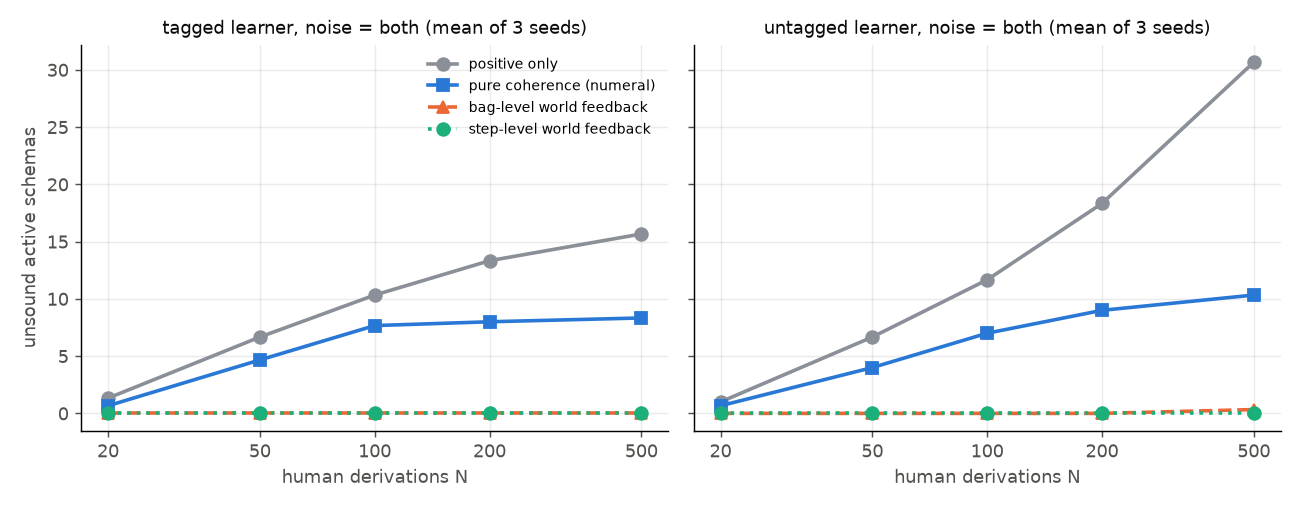
\includegraphics[width=0.85\textwidth]{../code/results/algebra_unsound.png}}
\caption{Experiment A: unsound active schemas against the number of human derivations $N$ (noise \texttt{both}, mean of three seeds), tagged learner (left) and untagged learner (right) \status{computed}. Imitation alone (grey) gets worse with $N$; coherence without a world (blue) removes about half; world feedback (orange, green) leaves one schema in one run.}
\label{fig:experiments:algebra}
\end{figure}

\paragraph{Coherence without a world converges to the meadow.} Pure coherence removes the errors that change the \emph{value} of a numeral expression. In paired runs of the tagged learner it deleted the freshman's dream in all 11 runs in which imitation had produced it, $(a+b)/(c+d)\to a/c+b/d$ in $17/17$ and $-(a+b)\to-a+b$ in $20/21$, and repaired unguarded $x/x\to1$ into the guarded rule in $31/35$. It almost never learned a guard that concerns only definedness: $a\cdot0\to0$ ended with a guard weaker than $\mathsf{defined}(a)$ in all 54 runs with $N\ge100$. Of the 90 pure-coherence runs, 88 end with an unsound schema (\Cref{fig:experiments:algebra}).

What survives has a meaning. Every unsound learned schema was re-tested in a \emph{total} semantics: complex values, $x/0:=0$, the principal square root, non-integer powers set to $0$. This is a version of the \emph{meadows} of \citet{bergstra2007rational}, and the convention of Lean's Mathlib (\cref{sec:philosophy}). All 41 target rules hold in it, all five fallacies fail in it, and seven of the 11 guards are unnecessary in it. For $N\ge200$, $304$ of the $315$ schemas that survive pure coherence ($96.5\%$) are sound in it. Of the other eleven, ten mention an object constant (as in $x\cdot z\to x$; pure coherence compares only numeral expressions) and one is a value error. For $N<200$ the share is $86.3\%$, since a smaller calculus derives fewer contradictions. Conversely, apart from one run, the guards that pure coherence \emph{did} learn are guards the total semantics also needs: $x/x\to1$ and $\sqrt{x^2}\to x$ came out exact whenever learned in general form, and in Experiment~C the coherence-only calculus guards $\sqrt{ab}\to\sqrt a\sqrt b$ in every seed by exactly the one atom, $\mathsf{nonneg}(a)$, that the total semantics requires. So pure coherence converged, not to the intended partial calculus, but to a coherent calculus for another meaning of ``$/$'' and ``$\sqrt{\ }$''. This is the algebraic counterpart of the Kripkensteinian residue of \Cref{thm:coherence:residue}: a coherent uniform alternative that agrees with everything positive examples and contradictions can supply. Only a channel that observes ``undefined'', here the world oracle at the corner point $x=0$, separates the two meanings (\Cref{ex:setting:alg2}).

\paragraph{Checks.} Soundness of schemas is a random test with 250 assignments that include undefined and irrational values. The review re-tested every active schema of five final calculi with $20{,}000$ random assignments plus a grid of special values and found no unsound one. Fresh seeds $3,4,5$ ($N=200$) reproduce the pattern: 14 to 15 unsound schemas after imitation, 8 to 9 after pure coherence, none after world feedback.

% ---------------------------------------------------------------------
\subsection{B: natural deduction, Post probes and the bold extension of IPC}\label{sec:experiments:prop}

\paragraph{Setup.} Formulas use atoms $p,q,r$ ($s$ only out of distribution) and $\to,\wedge,\vee,\neg,\bot$; steps are sequent-style natural-deduction inferences (\Cref{ex:setting:nd}). The target is classical natural deduction with 13 rules, the assumption rule carrying the side condition $A\in\Gamma$ as a $\mathsf{mem}$ guard; $\IPC$ drops reductio. Simulated humans prove random tautologies backwards. Their fallacies, each taken with probability $0.3$ and cited as ${\to}$E, are affirming the consequent (AC), denying the antecedent (DA) and an illegitimate discharge (ID); \texttt{noise} corrupts $5\%$ of steps. The learner \texttt{vs} buckets steps by cited rule, anti-unifies them under an MDL criterion, adds most-specific $\mathsf{mem}$ guards and verifies with support $m=2$. Coherence pruning uses five designated contexts: $\emptyset$ and four satisfiable premise sets. Negative bags (\Cref{lem:coherence:bag}) come from blind search for $\Gamma_d\der\bot$ and from \emph{Post probes}, which substitute $\bot$ or $\neg\bot$ for a rule's metavariables, prove its premises and refute its conclusion (\Cref{prop:search:post,lem:twotier:post}). Blame is a minimum-weight hitting set, weighted by the human steps the cheapest repair loses. The \texttt{world} phase adds two observed valuations of the 16. Rule soundness is decided exactly by truth tables. An adversary searches with the learned rules for derivations of 34 invalid goals, $\der\bot$ among them; \emph{sound completeness} is the share of 25 random tautologies the sound active rules prove within budget (target calculus: $0.88\pm0.03$).

\begin{table}[ht]
\centering\footnotesize
\setlength{\tabcolsep}{3.5pt}
\begin{tabular}{@{}lccccccc@{}}
\toprule
phase & unsound & tonk-like & exploits /34 & $\der\bot$ & rules /13 & sound compl. & world queries\\
\midrule
imitation only & $45.6\pm19.3$ & $30.2\pm12.2$ & $34.0\pm0.0$ & 9/9 & 13.0 & $0.87\pm0.04$ & 0\\
+ coherence, no world & $1.2\pm0.9$ & $0.0$ & $1.7\pm4.1$ & 0/9 & 13.0 & $0.87\pm0.04$ & 0\\
+ sparse world & $0.2\pm0.4$ & $0.0$ & $0.0$ & 0/9 & 13.0 & $0.87\pm0.04$ & $910\pm309$\\
\bottomrule
\end{tabular}
\caption{Experiment B, learner \texttt{vs}, noise \texttt{both}, $N\in\{50,100,200\}$: 9 runs, sd over the 9 runs \status{computed}. \emph{Tonk-like}: unsound rules whose conclusion is unconstrained by the premises; $\der\bot$: runs in which the adversary derives $\der\bot$; \emph{rules}: target rules recovered exactly or with a stronger guard. Held-out invalid steps accepted: $0.86\pm0.02$, $0.00\pm0.01$, $0.00$.}
\label{tab:experiments:prop}
\end{table}

\paragraph{Imitation, coherence, world.} Imitation recovers all 13 rules, but on noisy data MDL anti-unification merges corrupted steps that share a skeleton into tonk-like rules \citep{prior1960runabout}, and the adversary proves all 34 invalid goals (\Cref{tab:experiments:prop}). Coherence alone cuts the unsound rules from $45.6$ to $1.2$ and closes every route to $\der\bot$, at no cost in completeness. Over all 72 runs of \texttt{vs} ($N$ from 5 to 200, four noise settings), 47 runs have an unsound rule after imitation, 19 after coherence and 6 after world feedback, and $\der\bot$ is derivable in 32, 0 and 0. On clean data no phase has an unsound rule for $N\ge50$, and the assumption rule's side condition is learned from positives, as most specific guard. A fallacy counts as surviving if an active unsound rule licenses it or a special case of it. For $N\ge50$, AC survives imitation in all 18 runs with fallacies, DA in 14 and ID in 10, and coherence removes all of them except one closed instance of DA that mentions atoms, outside the structural hypothesis of \Cref{cor:coherence:fallacies}; world feedback removes that one too. At $N\le10$ coherence leaves unsound rules in 4 of 18 runs, AC itself among them: a small learned calculus may lack the rules needed to \emph{derive} the contradiction. Plotkin's learner without clustering (\texttt{aggressive}, 18 runs) produces $4.8\pm2.3$ tonk-like rules per run and lets the adversary derive $\der\bot$ in every run; after pruning, in none. Blame needs a prior (\Cref{thm:twotier:blame}): for this learner at $N=50$ on noise \texttt{both}, blaming the least-supported rule recovers $0.3\pm0.5$ target rules and no completeness, while blaming by cost of the cheapest repair recovers all 13 with completeness $0.87\pm0.04$.

\paragraph{Post-completeness probes.} A \emph{bold} learner over classical natural deduction adds a candidate schema iff no derivation of $\der\bot$ is found with it. Of 177 structural candidates (19 hand-picked, 8 pairwise LGGs of target rules, 150 random), the 59 classically valid ones were all accepted, and the 118 invalid ones were all refuted by an explicit derivation of $\der\bot$, as \Cref{thm:coherence:post,thm:coherence:cpc} predict. The derivations are short: median $2.5$ and maximum $6$ steps for the LGGs of target rules, median $6$ and maximum $17$ for the random schemas. For AC, the probe $A:=\bot$, $B:=\neg\bot$ gives
\[
\bot\der\bot\ (\text{ax}),\quad \bot\der\neg\bot\ (\neg\text{I}),\quad \der\bot\to\neg\bot\ ({\to}\text{I}),\quad \der\neg\bot\ (\neg\text{I}),\quad \der\bot\ (\text{AC}).
\]
Non-structural rules escape (\Cref{prop:twotier:structurality}): $\der p$ is coherent with every designated context and falls only to an observed valuation, and $p\der q$ falls to the designated context $\{p,\neg q\}$. Of the 45 unsound rules that survive pruning in any run, 38 mention specific atoms. Offered tonk's two rules one at a time, the bold learner accepts whichever comes first and rejects the other (\Cref{prop:coherence:tonk}). One observed valuation is a complete test for a schematic rule with $k$ metavariables only if all $2^k$ literal instantiations are probed. The code probes at most eight, and the three schematic rules that survive the world phase in some run each have $k\ge4$; probing all instantiations removed them. What world feedback adds is exact blame, since a refuted step names its rule: $5.0\pm2.1$ pruning rounds against $9.1\pm5.9$ without it ($N\ge20$, 36 runs).

\paragraph{The bold extension of intuitionistic logic.} Over intuitionistic natural deduction the bold learner accepted excluded middle, double-negation elimination, reductio, Peirce's law, weak excluded middle and Dummett's linearity, each underivable in $\IPC$ (a Kripke countermodel was found for each), and rejected the classically invalid candidates by derivations of $\der\bot$. Completeness on classical tautologies rose from $0.72$ to $0.80$ (classical natural deduction: $0.84$). The same happens when $\IPC$ is first \emph{learned}: from 60 simulated intuitionistic proofs, \texttt{vs} with coherence recovers the 12 rules (10 exactly, 2 with a stronger guard), never learns reductio, has no classically or Kripke-unsound rule, and its bold phase then accepts the same six principles. This is \Cref{thm:coherence:ipc}: coherence cannot separate the intermediate logics, so a maximal coherent structural learner never outputs $\IPC$, and the residue of \Cref{thm:coherence:residue}(ii) shows up as a drift toward $\CPC$. Only the cautious, imitation-based tier keeps $\IPC$.

\paragraph{Caveats.} The designated contexts are certified satisfiable with ground-truth satisfiability, a modelling assumption (\Cref{asm:setting:WS}), and ``coherent'' means that no derivation of $\bot$ was found within budget. Most-specific guards make $\wedge$E and $\vee$E stronger than the target, since the simulated humans only eliminate from open assumptions: sound, but incomplete out of distribution. Fresh seeds 3 and 4 ($N=50$, \texttt{both}) reproduce the pattern.

% ---------------------------------------------------------------------
\subsection{C: an adversarial prover against statistical and rule-learned verifiers}\label{sec:experiments:adversarial}

\paragraph{Setup.} All verifiers are trained on the same $N=500$ noisy algebra derivations of Experiment~A, except one trained on a clean corpus. The statistical verifiers, akin to process reward models, are logistic regression, gradient-boosted trees and a random forest on hashed subterm-shape $n$-grams, rule signatures and tree-edit features. They receive oracle labels for positives and for negatives (refuted human steps, perturbations, fallacy instances), so they get \emph{more} supervision than the positive-only rule learner. Thresholds are calibrated in distribution to a balanced precision $\mathrm{TPR}/(\mathrm{TPR}+\mathrm{FPR})$; ``$@\mathrm pX$'' means precision $X$. The rule-learned verifiers are A's learner without guards (\texttt{lgg\_pos}), with most-specific guards (\texttt{lgg\_ms}; \texttt{lgg\_ms\_clean} on the clean corpus), after pure coherence, and after world feedback; the ground-truth calculus is a control. The prover sees only accept or reject. It runs a bidirectional best-first search whose proposals are target rules, fallacies and near-miss schemas with guards ignored, arithmetic, random mutations, and goal-directed leaps and grafts, with 3000 verifier queries for each of 23 false goal equations and 1500 for each of 33 true identities. A derived equation counts as false when exact evaluation at 5 fixed points refutes it, so these counts are lower bounds.

\begin{table}[ht]
\centering\footnotesize
\setlength{\tabcolsep}{4pt}
\begin{tabular}{@{}lccccc@{}}
\toprule
verifier & ID bal.\ prec. & ID recall & false goals /23 & true goals /33 & false eq./$10^3$ q.\\
\midrule
boosted trees, threshold $0.5$ & $0.9752\pm0.0048$ & $0.958\pm0.003$ & $22.3\pm0.9$ & $31.0\pm0.0$ & $281.0\pm46.9$\\
boosted trees $@\mathrm p0.99$ & $0.9925\pm0.0049$ & $0.885\pm0.030$ & $16.3\pm2.4$ & $28.3\pm1.7$ & $259.2\pm45.7$\\
boosted trees $@\mathrm p1.0$ & $1.0000\pm0.0000$ & $0.450\pm0.048$ & $1.7\pm0.5$ & $4.7\pm0.5$ & $43.4\pm14.5$\\
random forest $@\mathrm p0.99$ & $0.9918\pm0.0014$ & $0.796\pm0.018$ & $13.0\pm0.8$ & $24.0\pm2.2$ & $168.0\pm30.2$\\
logistic regr.\ $@\mathrm p0.99$ & $0.9749\pm0.0209$ & $0.061\pm0.060$ & $3.3\pm1.9$ & $1.7\pm1.7$ & $104.4\pm35.8$\\
\addlinespace
\texttt{lgg\_pos} (no guards) & $0.9064\pm0.0057$ & $1.000\pm0.000$ & $20.7\pm0.9$ & $32.3\pm0.5$ & $269.0\pm41.3$\\
\texttt{lgg\_ms} (most-specific guards) & $0.9158\pm0.0052$ & $0.995\pm0.002$ & $14.0\pm0.8$ & $32.3\pm0.5$ & $141.2\pm7.6$\\
\texttt{lgg\_ms\_clean} (clean corpus) & $1.0000\pm0.0000$ & $0.988\pm0.005$ & $0.0\pm0.0$ & $32.3\pm0.5$ & $0.0\pm0.0$\\
LGG + coherence, no world & $1.0000\pm0.0000$ & $0.997\pm0.001$ & $5.0\pm0.0$ & $32.3\pm0.5$ & $98.7\pm8.4$\\
LGG + world (bag or step) & $1.0000\pm0.0000$ & $0.997\pm0.001$ & $0.0\pm0.0$ & $32.3\pm0.5$ & $0.0\pm0.0$\\
ground-truth calculus & $1.0000\pm0.0000$ & $0.997\pm0.001$ & $0.0\pm0.0$ & $32.3\pm0.5$ & $0.0\pm0.0$\\
\bottomrule
\end{tabular}
\caption{Experiment C: in-distribution metrics on held-out human-like steps, and outcomes under black-box adversarial search, three seeds \status{computed}. Bag- and step-level world feedback give identical rows. Six further statistical configurations are in \texttt{code/results/adversarial\_prover.md}.}
\label{tab:experiments:adversarial}
\end{table}

\paragraph{Accuracy in distribution does not transfer to the search distribution.} The boosted-tree verifier reaches test AUC $0.995$ on held-out human-like steps. Calibrated to in-distribution balanced precision $0.9925$, it still lets the prover prove $16.3\pm2.4$ of the 23 false goals, with a median of 514 queries to a false proof (\Cref{tab:experiments:adversarial}). At the strictest threshold, with no false accept on the calibration set, recall falls to $0.45$; it then proves $4.7$ of 33 true identities, and still $1.7$ false goals. All 11 statistical configurations derive false equations under search. Of their 1082 invalid proof edges, $81\%$ come from goal-directed leaps, grafts and random mutations, and only $1\%$ from the known fallacies: steps that look like human steps and are not. \Cref{fig:experiments:goodhart} plots the probability of a false proof against the budget and against in-distribution precision. This is \Cref{thm:search:tonk} and \Cref{lem:search:commitment}(ii) in a closed domain: in-distribution accuracy is a property of a measure fixed before the prover moves, soundness a property of a set. That learned reward models are exploited by optimization is documented at scale, notably by the overoptimization scaling laws of \citet{gao2023scaling}; the experiment adds a domain in which every exploited step can be certified invalid.

\begin{figure}[ht]
\centering
{\graphicspath{{./}{../../}}%
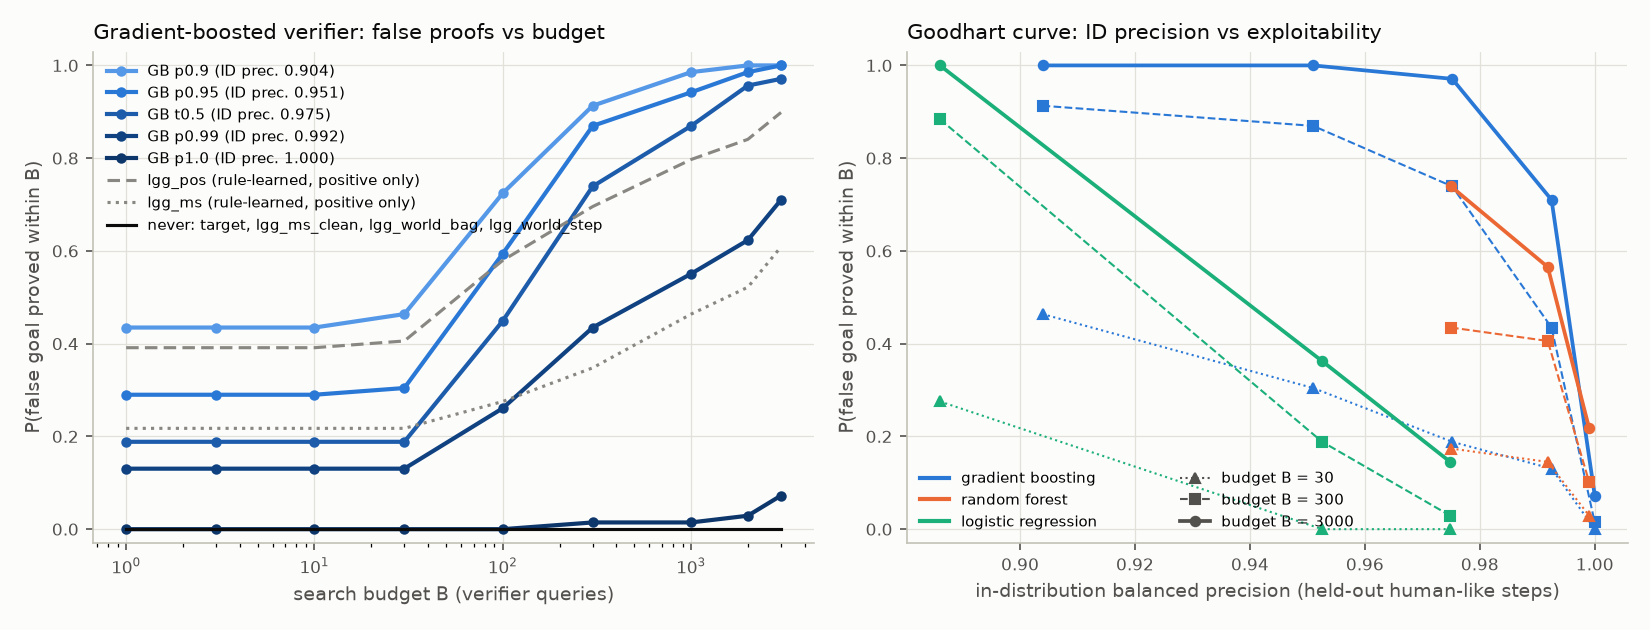
\includegraphics[width=0.95\textwidth]{../code/results/adversarial_prover_goodhart.png}}
\caption{Experiment C \status{computed}. Left: fraction of the $3\times23$ (seed, false goal) searches that found a false proof within $B$ verifier queries, for boosted trees at five thresholds and the positive-only rule learners; the ground-truth calculus, \texttt{lgg\_ms\_clean} and the world-repaired calculi never do. Right: the same probability at budgets 30, 300 and 3000 against in-distribution balanced precision.}
\label{fig:experiments:goodhart}
\end{figure}

\paragraph{Rule-learned verifiers fail only through named schemas.} All 154 invalid proof edges of the rule-learned verifiers are licensed by a schema that the soundness test flags; the most used is the noise-born projection $x+y\to y$, which alone collapses arithmetic ($1=1+1=2$). A counterexample deletes or guards such a schema and removes its whole family of exploits; a classifier has no such unit of repair. After world feedback the learned calculus proves no false goal and $32.3$ of 33 true identities, like the ground-truth calculus. With clean data and an adequate guard language positive data suffice: \texttt{lgg\_ms\_clean} proves no false goal, as the version-space verifier of \Cref{thm:caution:vs} should, although in one seed an over-specialized schema $0/(y+3)\to0$, whose true guard the guard language cannot express, is active and was not reached. Together, the four rule-based verifiers with no false goal derive no false equation in $900{,}305$ queries. Coherence without a world leaves A's residue: in-distribution balanced precision $1.0000$, yet 5 false goals per seed, all definedness errors such as $0/x=0$ and $(x-x)/y=0$, each true when $1/0=0$. In-distribution precision does not rank verifiers by soundness, even among rule-based ones.

\paragraph{Patching the classifier with its own exploits.} The natural remedy is adversarial data collection, as for PRM800K \citep{lightman2023verify}: harvest the certainly invalid accepted steps from the searches on the 23 false goals, add them as negatives, retrain and recalibrate. Over four rounds (boosted trees at $\mathrm p0.99$, seeds 0 and 1 only), false goals proved on the harvested set fell from $15.5$ to $0.0$ and false equations per thousand queries from $195.7$ to $14.3$. The patched verifier still proved $1.5$ of 12 fresh false goals and $2.0$ of 35 goals against a second, differently configured prover, while true identities proved fell from $28.0$ to $24.5$. Retraining is an effective practical mitigation; its soundness is relative to the attacks it was patched against. All of this is one small closed domain, an informed black-box prover (``not proved'' is not ``unprovable'') and small baselines on hand-built features; the experiment does not measure how often larger learned verifiers are exploited, and the theorems do not predict that rate.

% ---------------------------------------------------------------------
\subsection{D: the two-tier learner}\label{sec:experiments:ttl}

\texttt{ttl\_sim.py} runs the two-tier learner on a propositional practice with nine genuine and four fallacious tagged rules and $1\%$ sporadic noise, against a prover that enumerates and truth-table checks every step over ten formulas; re-running it reproduced \Cref{tab:twotier:sim} exactly \status{computed}. The positive-only cautious tier is unsound in 72 of 80 runs (\Cref{prop:twotier:practice}); the two-tier learner is unsound in none and exact in all 40 runs with $N\ge250$ (\Cref{thm:twotier:main,cor:twotier:cpc}). Only the singleton-conflict case of $\CPC$ with a per-schema world audit is simulated; Experiment~B is a related pipeline, not an implementation of the two-tier learner.

% ---------------------------------------------------------------------
\subsection{E: a physics mini-checker}\label{sec:experiments:physics}

\texttt{sps\_checker.py} runs the checks of \Cref{def:physics:checker} on the chair-leg solution of \Cref{sec:physics:example}; \Cref{tab:physics:checkerrun} lists the outcomes, which a re-run reproduced \status{computed}. The honest solution is accepted with certified error at most $0.0888$ within its $10\%$ tolerance, and all twelve variants are rejected, one of them (the honest solution with a $5\%$ tolerance) as a completeness gap. The first version of the checker \emph{accepted} four simple attacks (V6--V9) until each syntactic check was made semantic: relative soundness (\Cref{thm:physics:relative}) is only as good as the checks, a small instance of the lesson of \Cref{sec:search}.

% ---------------------------------------------------------------------
\subsection{F: simplicity}\label{sec:experiments:simplicity}

Five scripts check the quantitative claims of \Cref{sec:simplicity} (\Cref{tab:experiments:simplicity}), and each confirms its statement: a simplicity penalty with private randomness separates a good model from memorized errors on a window of steepness $c$, but it is blind to validity, so with realistic rates no $c$ keeps every valid rule and removes every error.

\begin{table}[ht]
\centering\footnotesize
\begin{tabularx}{\textwidth}{@{}l>{\raggedright\arraybackslash}X>{\raggedright\arraybackslash}p{0.19\textwidth}@{}}
\toprule
script & computed outcome & checks\\
\midrule
\texttt{c1} & The note's example: rates $8.99\cdot10^{-3}$ (model) and $1.12\cdot10^{-6}$ (error); the good model wins on a window of $c$ spanning a factor $8037$; standard MDL switches to the error model at $N=894{,}054$. & \Cref{cor:simplicity:example}\\
\texttt{c2} & Parities on $\{0,1\}^{10}$, $N=200$: per-input mixture $200.0$ bits, shared mixture $10.00$. With 16 errors, a product model one bit short has risk $0.546$ against $0.116$; shared-randomness code lengths stay in $[0.116,0.126]$: a kink only with private randomness. & \Cref{thm:simplicity:pricing,thm:simplicity:kink}\\
\texttt{c3} & Threshold rule: $0$ violations in $6000$ (instance, $c$) pairs; no minimizer off the lower hull; product optimum $=$ product of local optima. & \Cref{thm:simplicity:separable,lem:simplicity:hull}\\
\texttt{c4} & Rules toy: affirming the consequent (rate $5.42\cdot10^{-3}$) outranks reductio, cases, ex falso and induction, so simplicity alone has no good window; with coherence, Post and world filters, $c\in(9.04\cdot10^{-6},1.21\cdot10^{-4})$ removes all but conditional perfection, the residue. The cancellation guard is dropped for $c>1.81\cdot10^{-4}$. With ${\to}$I rare, the coherent optimum at $c=5\cdot10^{-4}$ sacrifices ${\to}$I to keep AC. Held-out log-loss is minimized by the smallest $c$. & \Cref{tab:simplicity:toy}, \Cref{thm:simplicity:blind,prop:simplicity:guard,prop:simplicity:sacrifice,thm:simplicity:validation}\\
\texttt{c5} & With two or more error contexts per block, an $O(1)$-bit in-context copier beats the norm model on every error context ($3.03$ against $4.64$ bits at two, $1.33$ against $4.68$ at sixteen). & \Cref{prop:simplicity:block}\\
\bottomrule
\end{tabularx}
\caption{Experiment F: the scripts \texttt{research/theory/T5-checks/c*.py}, re-run \status{computed}.}
\label{tab:experiments:simplicity}
\end{table}

% ---------------------------------------------------------------------
\subsection{G: the comprehension toy}\label{sec:experiments:comprehension}

\texttt{comprehension\_toy.py} runs the repair setting of \Cref{def:informal:repair} on the menu of \Cref{tab:informal:menu} \status{computed; re-run}. As a sanity check of \Cref{lem:informal:facts}, positive comprehension has the model $u\in u$, and none of the seven menu sets proved inconsistent by hand (Russell's set alone, and the pairs and triples behind (F5)) has a model with at most three elements, which is consistent with the lemma but no proof of it. For every practice the unconstrained MDL choice is naive comprehension, Frege's Basic Law~V, which coherence refutes. The coverage-maximal coherent repair then follows the practice, as \Cref{thm:informal:frz}(iv) states:

\begin{center}\footnotesize
\begin{tabular}{@{}lccccl@{}}
\toprule
practice (weights) & POS & STRAT & SEP & Z & selected\\
\midrule
INT 5, UNI 5, PAIR 3, DIFF 4, EMP 1 & 13 & 18 & 9 & 18 & STRAT (tie, broken by $\ell$)\\
\quad + V 1 (Frege's universal extension) & 14 & 19 & 9 & 18 & STRAT\\
\quad + ZR 3 (Zermelo's diagonal subsets) & 14 & 19 & 12 & 21 & Z\\
\quad same, with V 4 & 17 & 22 & 12 & 21 & STRAT\\
\bottomrule
\end{tabular}
\end{center}

\noindent The entries are coverages. On the Dedekind--Cantor operations stratification and separation tie and description length decides; once diagonal subsets outweigh the universal set, Z wins; reverse the weights and stratification wins. The theorem's full case analysis (93 sub-supports) is checked separately by \texttt{T4-checks/run\_all.sh}.

% ---------------------------------------------------------------------
\subsection{What the experiments do and do not show}\label{sec:experiments:limits}

They show the mechanisms of the theorems at work in small, fully checkable domains: positive data fix shapes but not guards (A, B); systematic errors reach support (A, B, D); coherence refutes uniform errors through Post's substitution and leaves a residue of coherent alternative meanings (the meadow in A and C, intermediate logics in B); a world channel that can see the residue removes it (A--C); and accuracy in distribution says nothing about soundness under search (C). They show no more than that. \emph{Realizability is assumed}: valid human steps are exact instances of the target rules, the guard language contains the true guards, and the simulated humans are the target plus known fallacies and noise; real practice satisfies none of this (\Cref{sec:informal}). \emph{Soundness is measured, not proved}: in A and C it is random testing, and ``0'' means that no counterexample was found; B decides rule soundness exactly, but its coherence verdicts and adversaries are budgeted searches. \emph{World feedback is cheap in algebra}: random evaluation is an almost perfect oracle for polynomial identities, and a run of A uses about $10^4$ queries; in physics, and in mathematics with undecidable fragments, B's two observed valuations or the certified bridges of \Cref{sec:physics} are the more realistic picture. \emph{Few seeds}: three per configuration (two for C's retraining), although fresh seeds reproduce the patterns of A and B. \emph{Toy scale}: closed small domains, heuristic and informed adversaries, small statistical baselines. Nothing here measures how often large neural verifiers are exploited, only why accuracy cannot rule it out.

\paragraph{Reproduction.} Python~3.11 with numpy, scipy, scikit-learn, matplotlib, mpmath and pytest (sympy for some checks). The full-grid JSON results are checked in, and \texttt{--report-only} rebuilds every report and plot of A--C from them in seconds; \texttt{--quick} runs a smoke test of each in one to two minutes. Wall-clock times on a shared 4-core machine:
{\small
\begin{verbatim}
cd code
python3 -m pytest -q                             # 85 tests, 1.5 min
./run_all_quick.sh                               # everything quick, 16 min
python3 experiments/exp_algebra_learning.py      # A, 19 min, 3 workers
python3 experiments/exp_prop_learning.py --workers 6         # B, 58 min
python3 experiments/exp_adversarial_prover.py    # C, 22 min
python3 experiments/exp_adversarial_prover.py --retrain      # 14 min
cd ../research/theory
(cd T7-checks && python3 ttl_sim.py)             # D, 22 s
(cd T3-checks && python3 sps_checker.py)         # E, 1 s
(cd T5-checks && for f in c?_*.py; do python3 $f; done)      # F
(cd T4-checks && python3 comprehension_toy.py)   # G
\end{verbatim}
}
\noindent \texttt{code/README.md} lists every script with its reproduction status in the review.

\section{Justification beyond proof}\label{sec:philosophy}

The investigation began with a question about principled justification. What does it look like, once we go beyond mathematical proof? This section steps back from the theorems and says what they show about that question. It also says what they do not show. Throughout, ``we'' means the authors of this report. The view argued for is deliberately modest. The theorems do not deliver a theory of justification. They make precise one shape that justification can take, and they locate exactly where that shape runs out.

\subsection{The setup is Goodman's circle, made into a learning problem}\label{sec:philosophy:goodman}

The setup we studied has three parts:
\begin{itemize}
\item learn inference rules from accepted inferences;
\item revise them when they generate unacceptable conclusions;
\item revise accepted inferences when they conflict with rules one is unwilling to give up.
\end{itemize}
This is, almost verbatim, Goodman's account of the justification of deduction and induction:
\begin{quote}
``Rules and particular inferences alike are justified by being brought into agreement with each other. \emph{A rule is amended if it yields an inference we are unwilling to accept; an inference is rejected if it violates a rule we are unwilling to amend.}'' \citep[ch.~III]{goodman1955fact}
\end{quote}
In our vocabulary, the channels correspond to Goodman's account as follows:
\begin{itemize}
\item Imitation (P) supplies the accepted particular inferences.
\item Rule schemas, learned by least generalization, are the rules.
\item Coherence (C) is the mechanism by which a rule ``yields an inference we are unwilling to accept''. A derivation of $\bot$ from a context certified consistent is a negative bag, and some rule in it must go.
\item World feedback (W) adds a channel whose errors are independent of human errors.
\end{itemize}
Without (W), the process is \emph{narrow} reflective equilibrium. With (W) it is \emph{wide} reflective equilibrium in the sense of \citet{daniels1979wide}. Daniels' ``independence constraint'' is, formally, the conditional-independence assumption that the coherence impossibility theorems show to be necessary (\cref{sec:coherence:eliminative}).

What our theorems add to Goodman's picture is a set of \emph{vindications with explicit conditions}. Under stated channel assumptions, mutual adjustment is \emph{sound against every adaptive arguer}, with explicit costs:
\begin{itemize}
\item realizability of the target in a structured hypothesis class;
\item truthful designation of the contexts that are certified consistent;
\item a world channel of the right kind.
\end{itemize}
For each assumption there is a matching impossibility result showing that dropping it breaks the guarantee (\cref{sec:twotier}). This is the sense in which the theorems are \emph{conditional reliabilist meta-justifications} of reflective equilibrium. They are not a non-circular foundation for logic. As \citet{dummett1973justification} observed, any justification of deduction is explanatory rather than suasive: it uses deduction. What they provide is an explicit list of what the process relies on, together with proofs that it relies on nothing else.

Two features of the guarantees matter philosophically.
\begin{itemize}
\item First, they are \emph{anytime}, not merely in the limit. Limit theorems are Reichenbachian vindications. They fall to the objection of \citet{salmon1967foundations} that infinitely many methods share the same limit while disagreeing at every finite stage. Our soundness guarantees hold at every time, with probability over the data (\cref{thm:caution:ville}). Our costs are explicit finite quantities: escalations, detections, samples. This also matches a recurring theme in the notes that prompted this work: suspicion of limit framings, and the view that thinking and mathematics are ``infinite endeavors'' with no final formula.
\item Second, they are \emph{worst case over arguers}. A step checker that is accurate on the distribution of human steps can be exploited by search (\cref{thm:search:tonk}). Justification that is to survive an untrusted or adversarial generator must be uniform over what the generator may propose. This is the case that motivates the question in the first place.
\end{itemize}

\subsection{What each signal can do, and the residue it leaves}\label{sec:philosophy:labour}

The main results combine into a division of labour. \Cref{tab:philosophy:labour} summarizes it.

\begin{table}[ht]
\centering\small
\begin{tabularx}{\textwidth}{>{\raggedright\arraybackslash}p{2.2cm}>{\raggedright\arraybackslash}X>{\raggedright\arraybackslash}X}
\toprule
Signal & What it provably fixes & What it provably cannot fix (residue)\\
\midrule
Imitation (P) & The \emph{rules} actually followed. Exact identification of a schematic calculus at coupon-collector rates (\cref{thm:imitation:coupon}), with systematic out-of-distribution generalization (\cref{cor:imitation:ood}). & Systematic errors, which are indistinguishable from rules at every rate (\cref{cor:imitation:systematic}). Imitation converges to ``competence'' in the sense of \citet{cohen1981irrationality}, not to validity \citep{stich1980justification}.\\
Cautious acceptance & Soundness against every adaptive arguer (\cref{thm:caution:vs,thm:caution:ville}). & Nothing new. It receives no coherence signal at all (\cref{prop:coherence:caution}), and its price is set by the structure of the class (\cref{tab:caution:cost}).\\
Coherence (C) & Every error that is incoherent with the target on a designated context (\cref{thm:coherence:elimination}). Exactly the target, for Post-complete targets: classical logic (\cref{thm:coherence:cpc}), and complete theories at the level of theorems. The classical \emph{meanings} of the connectives, once denials are allowed (\cref{thm:coherence:telltale}). & Coherent uniform alternatives: the Kripkensteinian residue (\cref{thm:coherence:residue}). Intermediate logics (\cref{thm:coherence:ipc}). $\Sigma_1$-unsound extensions of arithmetic (\cref{thm:coherence:popper}). Which valuation is actual.\\
Simplicity & Expensive, idiosyncratic errors, via a rate threshold (\cref{sec:simplicity}). & Cheap, frequent fallacies. Rare valid rules are lost. Its strength cannot be calibrated from imitation data.\\
World (W) & Objects give step-level blame by descent, so $\log_2|\Hc|$ corrections suffice, against $|\Hc|-1$ from paradoxes alone (\cref{thm:informal:objects,thm:informal:paradoxes}). Computation with fresh randomness gives worst-case-valid stochastic checks (\cref{lem:search:commitment}). Calibration of top models (\cref{sec:physics}). & Errors invisible on every presentable object. Effects outside the top model (\cref{thm:physics:judgment}).\\
Contexts & Reasoning under contradictory idealizations without explosion. Coherence where it belongs (\cref{thm:physics:realizability}). & The reading of a problem, and the adequacy of the top model. Both are ineliminable judgments (\cref{thm:physics:judgment}).\\
\bottomrule
\end{tabularx}
\caption{The division of labour among the learning signals, with the residue each one provably leaves.}\label{tab:philosophy:labour}
\end{table}

Two observations about this table seem to us to be the real philosophical content of the investigation.

\paragraph{Every signal is one-sided.}
Each learning signal we studied can refute errors in only one direction:
\begin{itemize}
\item Positive data never refute an over-generalization (Gold).
\item Coherence never refutes over-caution: a cautious learner never sees a contradiction (\cref{prop:coherence:caution}). Nor does it refute a coherent over-generalization (\cref{thm:coherence:silent}).
\item Coherence among exported tolerances never refutes a tolerance that is too wide. Widening an interval cannot create a contradiction (\cref{thm:physics:coherencetol}).
\item The demand that a problem be well posed refutes readings that are too wide, but it rewards readings that are too narrow (\cref{prop:physics:gricean}).
\end{itemize}
Each one-sided signal is an attack surface for an adversarial arguer, and it calls for a complementary signal that refutes errors in the other direction. Principled justification, on this picture, is not one master criterion. It is a set of signals that \emph{together} cover every direction of error, plus an explicit statement of the directions that remain uncovered. \Cref{tab:physics:onesided} lists the pairs for physics. The same structure appears in mathematics. Imitation proposes and caution guards. Coherence condemns, but only bold hypotheses. Objects localize.

\paragraph{Each residue has a name, and different philosophies disagree only about the residue.}
Outside the residue of coherent, uniform, world-adequate alternatives, every position we know of counts the learner as correct:
\begin{itemize}
\item the realist;
\item the Peircean, for whom truth is the limit of inquiry;
\item the Dummettian, for whom truth is warranted assertibility;
\item Carnap's tolerance;
\item Quine's pragmatism.
\end{itemize}
Inside the residue, they disagree. The realist sees undetectable error. The Peircean or Dummettian sees no fact of the matter. Carnap sees a free choice of language. Quine sees a choice made on pragmatic grounds. The theorems make the residue precise in several cases:
\begin{itemize}
\item It is empty for classical propositional logic.
\item It contains all intermediate logics for an intuitionistic practice.
\item It contains $\PA+\neg\Con(\PA)$ for arithmetic.
\item In the algebra experiment it contains the total semantics with $1/0=0$, which pure coherence converged to (\cref{sec:experiments}). This is, as it happens, exactly the convention adopted by Lean's Mathlib and by Isabelle/HOL, where $x/0=0$.
\end{itemize}
A theorem can say exactly where these philosophies part ways. It cannot settle who is right inside the residue. We think that is the correct division of labour between mathematics and philosophy here.

One consequence deserves to be stated on its own. \emph{Rules can be identifiable when truths are not.} The bilateral tell-tale identifies classical meanings from finitely many data (\cref{thm:coherence:telltale}). Yet no computable learner on the same channels decides $\Sigma_2$ truth in the limit (\cref{thm:coherence:popper}). This undercuts the simple form of Dummett's acquisition argument. That argument holds that a meaning one could acquire must be manifestable in use, so meaning cannot outrun decidability. But a learner can acquire the meaning-constitutive \emph{rules} exactly, while the truth values they determine remain beyond any computable reach.

\subsection{Rules are not premises}\label{sec:philosophy:carroll}

The tortoise of \citet{carroll1895tortoise} refused to infer $Z$ from $A$, $B$ and ``if $A$ and $B$ then $Z$'' until that inference was itself added as a premise, and so on forever. For a learner the lesson has a precise form:
\begin{itemize}
\item A learned \emph{rule} is a schema. Its validity is a universally quantified claim over all instances, of $\Pi$ form.
\item No finite amount of world feedback verifies such a claim. Feedback can only refute it.
\item The justification for \emph{using} a learned rule therefore cannot be further premises. It has to be a guarantee about the process that accepted it: cautious acceptance, and an anchor that has been observed.
\end{itemize}
This is why the right acceptance policy for learned rules is Popperian. Accept tentatively. Assert only what every surviving hypothesis licenses. Treat each refutation as permanent. It is also why self-certification must never feed back into acceptance:
\begin{itemize}
\item a learned verifier that ``proves its own soundness'' has provided no evidence that distinguishes it from an unsound verifier sharing the certifying rule;
\item in arithmetic, by Löb's theorem a theory that proves the reflection schema $\mathrm{Prov}_T(\ulcorner\varphi\urcorner)\to\varphi$ for its \emph{own} provability predicate, for all $\varphi$, proves everything. By contrast, the corresponding reflection \emph{rule} is admissible for $\Sigma_1$-sound theories.
\end{itemize}
Reflection is a principled source of genuinely new inferences, beyond imitation, that a learner who has accepted a calculus is committed to. Where it is used, it must enter as a stratified rule, never as a self-referential premise.

\subsection{What principled justification beyond proof looks like}\label{sec:philosophy:shape}

Putting the pieces together, the results suggest the following shape for a principled justification of a claim about something other than pure mathematics. A physics olympiad answer is the running case.

\begin{enumerate}
\item \textbf{Proof inside contexts.} Each step inside a context is checked against a calculus. The calculus is formal where possible. Where it is learned, acceptance is cautious, so the check is sound against an arguer who searches for weaknesses (\cref{sec:caution,sec:informal}).
\item \textbf{Certified bridges between contexts.} Moving a conclusion from an idealized context to the claim of interest is not a logical step. It needs a certificate carrying information of finite radius about how the quantity behaves away from the idealization. Facts about the idealized model alone never suffice (no free export, \cref{thm:physics:nofree}). Side conditions are evaluated where they are true, in the parent context, and contexts are declared deformations. Otherwise an arguer can ``stipulate'' its way to anything (\cref{thm:physics:stipulation}).
\item \textbf{An explicit judgment layer.} What remains is provably ineliminable (\cref{thm:physics:judgment}):
  \begin{itemize}
  \item that the problem was read correctly, i.e.\ the admissible worlds were not narrowed;
  \item that the top model is adequate for the world claims;
  \item that the trusted base is trustworthy.
  \end{itemize}
  A principled justification does not hide this layer. It minimizes it and declares it.
\item \textbf{Correctness as supertruth.} For underspecified questions, ``true in the context at hand'' means true in every admissible completion of the intended model, to the demanded precision. This is the largest acceptance criterion that stays sound under uncertainty about the reading (\cref{thm:physics:superval}). Answer-invariance under unspecified features, which experienced solvers notice and rely on, is exactly a certificate of supertruth.
\item \textbf{Learning signals with known limits.} Every learned component comes with a statement of the signal that trained it and the residue that signal leaves. The learned components are the calculus, the bridge validity regions and the tolerances.
\end{enumerate}

Measured against this shape, mathematical proof is the limiting case in which:
\begin{itemize}
\item the judgment layer has shrunk to the reading of the formal statement and trust in the axioms;
\item every bridge is exact;
\item the calculus is fixed rather than learned.
\end{itemize}
Informal mathematics before formalization sits in between. It was a bounded-gap practice over a latent calculus, as the robust-core hypothesis suggests. In it, counterexample objects did most of the corrective work, and paradoxes were rare and uninformative (\cref{sec:informal}). Physics adds a nonempty, explicit judgment layer and non-logical bridges, but the shape is the same. On this view the difference between mathematical and physical justification is one of degree, measured by the size of the declared residue, not one of kind.

\subsection{What this says about meaning}\label{sec:philosophy:meaning}

The inferentialist premise of the question was that learning which inferences are valid is roughly learning meanings. The results support a qualified version:
\begin{itemize}
\item \textbf{Inferential roles are learnable, exactly, from finite use.} A finite anchor fixes the inferential role of a vocabulary for unbounded use (\cref{cor:imitation:ood}). This is a precise, if modest, answer to the rule-following question of how finite training fixes an infinite norm. The answer is: through structure (schemas) plus a small set of telling instances. The skeptic's ``quus'' survives only as a non-uniform patch, which uniformity rules out, or as a coherent uniform alternative, which is a named residue.
\item \textbf{More than role is not identifiable.} Practice, coherence and object data identify a latent formalization exactly up to informal-validity equivalence, and no further (\cref{thm:informal:identify}). Ontology is not identifiable: standard and nonstandard reals are observationally equivalent on the practice (\cref{prop:informal:transfer}). Neither is the choice of set-theoretic reduction (\cref{prop:informal:benacerraf}).
\item \textbf{Coherence buys existence, but not intended existence.} Every coherent mode of talking has \emph{something} it could be talking about. That is a generalized completeness theorem, true for positions, credences and context systems alike (\cref{sec:existence}). But that something may be a syntactic or nonstandard model. Intended existence needs one of three additional things:
  \begin{itemize}
  \item categoricity;
  \item anchoring of the vocabulary to the world (Beth definability);
  \item an infinitary condition, such as the probabilistic $\omega$-rule.
  \end{itemize}
  None of these can be certified computably beyond $\Pi_1$.
\end{itemize}
Inferential role is one aspect of meaning, and the project captures that aspect precisely. Other aspects are not captured by anything studied here:
\begin{itemize}
\item the ``hooking'' of a conception onto the world;
\item the activities a concept supports;
\item the questions it lets one ask.
\end{itemize}
We do not claim otherwise.

\subsection{Answers to the questions that prompted the investigation}\label{sec:philosophy:answers}

The investigation was prompted by a set of questions. Most of them are recorded in notes that are publicly available. \Cref{tab:philosophy:answers} lists the main ones with pointers to where they are answered or partly answered.

\begin{table}[ht]
\centering\small
\begin{tabularx}{\textwidth}{>{\raggedright\arraybackslash}p{5.6cm}>{\raggedright\arraybackslash}X}
\toprule
Question & Where and how it is answered\\
\midrule
What is an appropriate learning algorithm for inference rules (learning from positive examples)? & Least generalization over schemas, with a trimmed version space for sporadic noise and cautious acceptance (\cref{sec:caution,sec:imitation}). MDL is the wrong bias for positive data (\cref{prop:search:mdl}).\\
Does that plus coherence get formal math working? & Yes for classical propositional logic and complete decidable theories (\cref{sec:coherence,sec:twotier}). Arithmetic is Popperian. There are sharp limits at $\Sigma_2$ and for Turing progressions.\\
Would a setup have worked before we knew how to formalize proofs? & A bounded-gap verifier over latent formalizations is sound against adaptive provers and identifies validity exactly up to informal-validity equivalence. Counterexample objects are exponentially more informative than paradoxes, and Frege$\to$Russell$\to$Zermelo comes out as constrained repair (\cref{sec:informal}). The hardest open problem is affordable soundness when the learner must invent language.\\
How should contexts be handled, and what about contradictory idealizations (``air pressure $=0$'')? & Contexts are filters of models, and coherence is enforced only on the root and anchored contexts (\cref{thm:physics:realizability}). Designating ``idealization + full background'' as coherent forces a globally paraconsistent logic (\cref{prop:physics:misdesignation}). Reductio needs a consistency certificate (\cref{thm:physics:hygiene}).\\
``Check that a claim is true in the context at hand. But wtf is that?'' & Supertruth: true in every admissible completion of the intended model, to the demanded precision (\cref{thm:physics:superval}).\\
Can physics olympiad solutions be checked in a principled way? & A structured-solution checker that is sound against adversarial solvers, relative to an explicit judgment layer that is provably ineliminable (\cref{thm:physics:relative,thm:physics:judgment}). There is a worked EuPhO example (\cref{sec:physics:example}).\\
Does a steeper simplicity penalty recover intended rules rather than teacher errors? & Partly. The kink intuition is vindicated for product models. But selection is a rate threshold with provable pathologies, and the threshold is not identifiable from imitation data (\cref{sec:simplicity}).\\
Is there a ``philosophical completeness theorem''? & Yes in the weak sense, and no in the intended sense (\cref{sec:existence}). Local coherence constraints of the kind used in consistency-based probing do not characterize coherence.\\
How come mathematicians ended up with such a nice notion of proof? & Through local checkability on objects, plus completeness, plus a bounded repertoire. Monster pressure leaves exactly the steps valid in every model of the theory, and Gödel completeness turns those into derivations (\cref{prop:informal:emergence}). Practice used only the robust core of its vague concepts (\cref{thm:informal:robust}).\\
\bottomrule
\end{tabularx}
\caption{The motivating questions and where they are addressed.}\label{tab:philosophy:answers}
\end{table}

\section{Limits and open problems}\label{sec:open}

We collect the main limitations of the results and the open problems they leave. The hardest of them is the first.

\paragraph{1. Affordable soundness when the learner must invent language.} Every soundness guarantee here is relative to \emph{realizability}: the target calculus, or the latent formalization, must lie in the hypothesis class. History did not respect any fixed class. It invented uniform convergence, ideals, $\varepsilon$--$\delta$ and the fundamental group as proof-generated concepts.
\begin{itemize}
\item A universal, language-inventing class restores realizability, but sound verification then costs on the order of $2^{K(h^*)}$ escalations (\cref{thm:caution:unstructured,thm:informal:escalation}).
\item What is needed is a class that is closed under the definitional extensions mathematics actually made, and that still has small escalation dimension. Equivalently, we need a theory of when concept invention, for example by anti-unification over definitions or by naming the hidden lemma found by descent, is cheap.
\end{itemize}

\paragraph{2. Computational cost.} Our bounds count samples, escalations, detections and refutation-oracle calls, not computation.
\begin{itemize}
\item Membership in the version-space intersection for untagged unions is likely NP-hard.
\item Consistency with negative bags is a multiple-instance problem. Its hardness is the formal shadow of the obfuscated-arguments problem in debate.
\item Refutation search is only semi-decidable. Our depth-relative soundness (\cref{thm:twotier:depth}) is the honest form of what can be had.
\end{itemize}
A complexity-theoretic version of the two-tier theorem would be valuable. It would identify which audits are polynomial and for which classes.

\paragraph{3. The reading layer.} In physics the irreducible judgment is the \emph{reading}: which admissible worlds the problem text determines (\cref{thm:physics:judgment}).
\begin{itemize}
\item Determinacy refutes only over-wide readings (\cref{prop:physics:gricean}).
\item What positive data identify the intended admissible class? We conjecture that official solutions together with marking schemes form a tell-tale within a class of ``minimal completions consistent with the intended imports''.
\item Learning readings soundly is, we think, the central open problem for principled checking beyond mathematics.
\end{itemize}

\paragraph{4. Sharp combinatorics.} Several bounds have gaps:
\begin{itemize}
\item The binomial conjecture for $k$-unions of intersection-closed classes (\cref{conj:caution:binomial}) would close the gap for untagged schema learning.
\item The bag-price conjecture $M_{\mathrm{bag}}^{(r)}\le r\cdot\mathrm{Ldim}$ (\cref{conj:informal:bagprice}) would give the exact exchange rate between paradoxes and counterexample objects.
\item The query complexity of sound blame, i.e.\ computing the union of the minimal conflicts with a conflict oracle, is open.
\end{itemize}

\paragraph{5. Coherence beyond Post-completeness.}
\begin{itemize}
\item For which first-order or modal targets does every invalid uniform rule have a short coherence witness in a natural designated context?
\item Is there a hierarchy of coherence-witness complexity?
\item Which logics and theories are \emph{coherence-pinned}, meaning that the residue is empty for natural families of designated contexts?
\item For arithmetic: is there a principled learner over reflection progressions that converges to ``the right amount of reflection'' under a natural feedback notion?
\end{itemize}

\paragraph{6. Simplicity and normativity.}
\begin{itemize}
\item For which classes of simple models does the product-model frontier kink, beyond parities?
\item Is there a principled, data-free choice of the simplicity coefficient, for example one tied to the cheapest postulate-violating error?
\item Which assumptions on a performance model, such as errors being time-bounded shortcuts, make joint description length identify competence despite the known non-identifiability of preferences from behaviour?
\end{itemize}

\paragraph{7. Probabilistic and contextual coherence.}
\begin{itemize}
\item Find a finitely presented proof system for valid counting sequents that is complete for de Finetti coherence.
\item Prove a probabilistic local-to-global theorem for context systems on tree covers.
\item Decide whether contextual frustration between idealized contexts should be penalized or tolerated.
\end{itemize}

\paragraph{8. Scale.}
\begin{itemize}
\item Our experiments are illustrations in small symbolic domains with realizable targets, cheap world feedback and few seeds.
\item Whether learned calculi with cautious acceptance remain affordable at the scale of real mathematical corpora (for example Lean or Metamath step data with injected fallacies at measured human rates) is an empirical question we have not addressed.
\item We have deliberately not built a strong prover, and we would recommend that any such work keep the checker separate from the generator.
\end{itemize}

\bibliographystyle{plainnat}
\bibliography{bib/all}
\appendix
% ===================================================================
% Appendix to Section 2 (Setting): proofs of the anti-unification lemmas.
% Source: research/theory/T1 §1.3 (Lemmas 1.2, 1.3; unchanged by verification).
% ===================================================================
\providecommand{\vars}{\mathrm{vars}}

\section{Proofs for Section~\ref{sec:setting}}\label{app:setting}

\Cref{thm:setting:lgg} is due to \citet{plotkin1970note} and
\citet{reynolds1970transformational}. All other statements of
\Cref{sec:setting} are proved here. The rank lemma and the recovery lemma are T1
Lemmas~1.2--1.3, which the referees reported correct with no change needed; the
other three are routine.

\subsection{Proof of \Cref{lem:setting:closure} (closure facts)}

(a) Let $D$ be the set of judgments with an $R$-derivation from $B$. $D$ contains
$B$ (one-node derivations) and is closed under $R$: if $P\step j\in R$ and
$P\subseteq D$, graft derivations of the finitely many members of $P$ under a new
root $j$. So $\Cl_R(B)\subseteq D$. Conversely, if $X\supseteq B$ is $R$-closed,
induction on the height of derivations shows that every node of every derivation
from $B$ lies in $X$; so $D\subseteq\Cl_R(B)$. Extensivity and monotonicity in
$B$ and in $R$ hold because a derivation from $B$ using steps of $R$ is also one
from any $B'\supseteq B$ using steps of any $R'\supseteq R$. Idempotence: a
derivation from $\Cl_R(B)$ becomes a derivation from $B$ after grafting a
derivation from $B$ above each leaf. Finitarity: a derivation has finitely many
leaves, so it is a derivation from a finite $B_0\subseteq B$.

(b) A single step $P\step j\in R$ is a derivation of $j$ from $P$, so
$R\subseteq\Sound(R)$, and monotonicity in the rule set gives
$\Cl_R(B)\subseteq\Cl_{\Sound(R)}(B)$. Conversely, $\Cl_R(B)$ is closed under
$\Sound(R)$: if $P\subseteq\Cl_R(B)$ and $j\in\Cl_R(P)$, then by (a)
$j\in\Cl_R(\Cl_R(B))=\Cl_R(B)$; it contains $B$, so it contains
$\Cl_{\Sound(R)}(B)$. Finally, $\Sound(A)=\{P\step j:j\in\Cl_A(P)\}$ depends
only on $\Cl_A$, so $\Cl_A=\Cl_R$ gives $A\subseteq\Sound(A)=\Sound(R)$; and
$\Sound(R)$ itself has the closure $\Cl_R$. \qed

\subsection{Proof of \Cref{lem:setting:rank} (rank)}

Throughout, $|t|$ is the number of symbol occurrences in $t$, metavariable
occurrences included, and $\vars(t)$ is the set of distinct metavariables of $t$.
A \emph{renaming} of a set $X$ of metavariables is a substitution whose
restriction to $X$ is an injective map into metavariables. If $\tau=\sigma\theta$
with $\theta$ a renaming of $\vars(\sigma)$, then $\sigma=\tau\theta^{-1}$, so
$\sigma\equiv\tau$; conversely, $\sigma\equiv\tau$ means equality up to such a
renaming, and then $\mu(\sigma)=\mu(\tau)$.

Let $\tau=\sigma\theta$. Let $x_1,\dots,x_k$ be the distinct metavariables of
$\sigma$, and let $x_i$ occur $m_i\ge1$ times in $\sigma$.

\emph{Size.} Replacing each of the $m_i$ occurrences of $x_i$ (one symbol) by
$\theta x_i$ (with $|\theta x_i|$ symbols) gives
\[
  |\tau|=|\sigma|+\sum_{i=1}^k m_i\big(|\theta x_i|-1\big).
\]

\emph{Metavariables.} Every metavariable of $\tau$ occurs in some $\theta x_i$, so
\[
  |\vars(\tau)|\le\sum_{i=1}^k|\vars(\theta x_i)|,
\]
with equality iff the sets $\vars(\theta x_i)$ are pairwise disjoint.

\emph{Difference.} Since $|\vars(\sigma)|=k$,
\begin{equation}\label{eq:app:setting:rank}
  \mu(\tau)-\mu(\sigma)
  \;\ge\;\sum_{i=1}^k\Big[m_i\big(|\theta x_i|-1\big)+1-|\vars(\theta x_i)|\Big].
\end{equation}
We bound each summand.
\begin{itemize}
\item If $\theta x_i$ is a metavariable, then $|\theta x_i|=1=|\vars(\theta x_i)|$
  and the summand is $0$.
\item Otherwise $\theta x_i$ contains at least one function or constant symbol and
  at least one occurrence of each of its metavariables, so
  $|\theta x_i|\ge|\vars(\theta x_i)|+1$. Using $m_i\ge1$, the summand is at least
  $(|\theta x_i|-1)+1-|\vars(\theta x_i)|\ge1$.
\end{itemize}
Hence $\mu(\tau)\ge\mu(\sigma)$.

\emph{Equality.} If $\mu(\tau)=\mu(\sigma)$, then every summand in
\eqref{eq:app:setting:rank} is $0$ and the inequality there is tight. The first
forces every $\theta x_i$ to be a metavariable; the second forces the sets
$\vars(\theta x_i)=\{\theta x_i\}$ to be pairwise disjoint, i.e.\ the
$\theta x_i$ to be pairwise distinct. So $\theta$ restricted to $\vars(\sigma)$ is
a renaming. Conversely, if it is a renaming, then $|\tau|=|\sigma|$ and
$|\vars(\tau)|=|\vars(\sigma)|$, so $\mu(\tau)=\mu(\sigma)$.

\emph{Chains.} Suppose $\sigma_{l+1}\succ\sigma_l$ strictly, i.e.\
$\sigma_l=\sigma_{l+1}\theta_l$ and $\sigma_l\not\equiv\sigma_{l+1}$. Then
$\theta_l$ is not a renaming of $\vars(\sigma_{l+1})$ (otherwise the two would be
equivalent), so $\mu(\sigma_l)>\mu(\sigma_{l+1})$, i.e.\
$\mu(\sigma_l)\ge\mu(\sigma_{l+1})+1$. Summing along
$\tau=\sigma_0\prec\sigma_1\prec\dots\prec\sigma_m$ gives
$\mu(\tau)\ge\mu(\sigma_m)+m$, and $\mu(\sigma_m)\ge0$. \qed

\subsection{Proof of \Cref{lem:setting:recover} (when the lgg recovers the schema)}

Let $\sigma$ have metavariables $x_1,\dots,x_v$, let $\theta_1,\dots,\theta_n$ be
ground substitutions ($n\ge1$), and let $t_j=\sigma\theta_j$. For each
metavariable $x$ of $\sigma$ write $c_x=(\theta_1x,\dots,\theta_nx)$ for its
\emph{column}, and let $\eta$ be the substitution $\eta(x):=\mathcal A(c_x)$.

\emph{Claim.} For every subterm $\sigma'$ of $\sigma$,
$\mathcal A(\sigma'\theta_1,\dots,\sigma'\theta_n)=\sigma'\eta$.

By induction on $\sigma'$. If $\sigma'=x$ is a metavariable, both sides are
$\mathcal A(c_x)$. If $\sigma'=f(\sigma'_1,\dots,\sigma'_r)$ (with $r=0$ for a
constant), then every $\sigma'\theta_j=f(\sigma'_1\theta_j,\dots,\sigma'_r\theta_j)$
has root $f$, so by definition $\mathcal A$ outputs $f$ applied to
$\mathcal A$ of the argument columns $(\sigma'_k\theta_1,\dots,\sigma'_k\theta_n)$,
which by the induction hypothesis are $\sigma'_k\eta$. Hence the output is
$f(\sigma'_1\eta,\dots,\sigma'_r\eta)=\sigma'\eta$.

Taking $\sigma'=\sigma$ and using \Cref{thm:setting:lgg},
\[
  \lgg(t_1,\dots,t_n)=\mathcal A(t_1,\dots,t_n)=\sigma\eta\preceq\sigma .
\]

\emph{When $\eta$ is a renaming.} By the definition of $\mathcal A$:
\begin{itemize}
\item $\eta(x)=\mathcal A(c_x)$ is a metavariable iff the entries of $c_x$ do not
  all have the same root, i.e.\ iff (R) holds at $x$. If (R) fails at $x$,
  $\eta(x)$ is a compound term or a constant.
\item If (R) holds at $x$ and at $y$, then $\eta(x)=z_{c_x}$ and $\eta(y)=z_{c_y}$,
  and these coincide iff $c_x=c_y$, i.e.\ iff (D) fails for the pair $x,y$.
\end{itemize}
So $\eta$ restricted to $\vars(\sigma)$ is a renaming iff (R) holds for every $x$
and (D) holds for every pair $x\neq y$.

\emph{Conclusion.} If (R) and (D) hold, $\eta$ is a renaming and
$\lgg(t_1,\dots,t_n)=\sigma\eta\equiv\sigma$. If either fails, $\eta$ is not a
renaming of $\vars(\sigma)$, so by \Cref{lem:setting:rank}
$\mu(\sigma\eta)>\mu(\sigma)$; since equivalent schemas have equal rank,
$\lgg(t_1,\dots,t_n)\not\equiv\sigma$, and it is strictly more specific. \qed

\subsection{Proof of \Cref{lem:setting:guard} (guarded closure)}

$P\subseteq\inst(\lgg(P))$ by \Cref{thm:setting:lgg}, and every $\phi\in\Psi_P$
holds on $P$, so $P\subseteq\inst(\lgg(P),\Psi_P)$. Let
$P\subseteq\inst(\sigma,\Psi)$. Then $P\subseteq\inst(\sigma)$, so
$\sigma\succeq\lgg(P)$ and $\inst(\lgg(P))\subseteq\inst(\sigma)$. Every
$\phi\in\Psi$ holds on all of $P$, so $\Psi\subseteq\Psi_P$ and
$\bigcap_{\phi\in\Psi_P}\phi^{-1}(1)\subseteq\bigcap_{\phi\in\Psi}\phi^{-1}(1)$.
Intersecting, $\inst(\lgg(P),\Psi_P)\subseteq\inst(\sigma,\Psi)$. \qed

\subsection{Proof of \Cref{lem:setting:WS} ((WS) and coherence)}

This is the remark following (WS) in T7 \S1.3, in the form repaired after
verification (without the clause $\Ttrust\subseteq\Sound(\Rstar)$). Write
$R^+=\Rstar\cup\Ttrust$. Let $\pos{\Gamma}{\Delta}$ be designated and $V$ as in
(WS). $V$ makes every member of $\Gamma$ true, and no step of $R^+$ has true
premises and a false conclusion, so the set of $V$-true judgments is an
$R^+$-closed superset of $\Gamma$ and contains $\Cl_{R^+}(\Gamma)$. Since $V$
makes $\bot$ and every member of $\Delta$ false, $\bot\notin\Cl_{R^+}(\Gamma)$
and $\Delta\cap\Cl_{R^+}(\Gamma)=\emptyset$. As $\Cl_{\Rstar}(\Gamma)\subseteq
\Cl_{R^+}(\Gamma)$ (\Cref{lem:setting:closure}(a), monotonicity in the rule set),
the position is also in bounds for $\Rstar$.

Conversely, let $J_W=\emptyset$ and let $\pos{\Gamma}{\Delta}$ be a designated
position that is in bounds for $R^+$. Then $e$ is well defined, because
$\Gamma\subseteq\Cl_{R^+}(\Gamma)$ is disjoint from $\Delta\cup\{\bot\}$. Let $V$
be the indicator function of $\Cl_{R^+}(\Gamma)$. It extends $e$: it is $1$ on
$\Gamma$ and $0$ on $\Delta\cup\{\bot\}$. The set $\Cl_{R^+}(\Gamma)$ is closed
under $R^+$, so no step of $R^+$ has $V$-true premises and a $V$-false conclusion,
and (WS) holds. For the parenthetical instance: if $\Ttrust\subseteq\Sound(\Rstar)$,
then $\Rstar\subseteq R^+\subseteq\Sound(\Rstar)$, so by
\Cref{lem:setting:closure}(a),(b) $\Cl_{R^+}=\Cl_{\Rstar}$, and being in bounds
for $\Rstar$ is the same as being in bounds for $R^+$. \qed

% =====================================================================
% Appendix: proofs for Section 3 (Search makes soundness a worst-case property)
% Sources: research/theory/T1-soundness-under-search.md (Cor 2.2, Prop 2.3 and its repair),
%          research/lit/L3-learning-to-reason-and-limit-inquiry.md (Lemma A, as repaired),
%          research/theory/T2-coherence-as-negative-data.md (Thm 2.4, as repaired),
%          research/verification/{T1,T2,L3}-*.md.
% =====================================================================
\providecommand{\Steps}{\mathrm{Steps}}

\section{Proofs for Section~\ref{sec:search}}\label{app:search}

\Cref{lem:search:stepwise}, \cref{thm:search:tonk}, \cref{prop:search:post} and \cref{prop:search:mdl} are proved in full in the main text. This appendix proves the remaining results of \cref{sec:search}, verifies the claims of \cref{ex:search:atoms}, and records the examples showing that the hypotheses of \cref{lem:search:commitment,thm:search:doctrinal} are needed. Notation is as in \cref{sec:search}; in particular $S$ is the set of all steps (\cref{def:setting:step}). Throughout, $\models$ is classical propositional consequence, and a step $\Pi\step\varphi$ over formulas is \emph{sound} if $\Pi\models\varphi$.

% ---------------------------------------------------------------------
\subsection{PAC learners can be maximally unsound}\label{app:search:pac}

\begin{proof}[Proof of \cref{cor:search:pac}]
For $N\ge0$ let $S_{\ge N}:=\{s\in S:|s|\ge N\}$.

\emph{Step 1: $T_j\subseteq S_{\ge j}$.} Every step of~$T_j$ has the premise $A\vee\top^{(j)}$, and $\top^{(j)}$ contains $j$ occurrences of~$\top$. So every step of~$T_j$ has size at least~$j$.

\emph{Step 2: the tail bound.} The sets $S_{\ge N}$ decrease in~$N$ and have empty intersection, so $Q(S_{\ge N})\downarrow0$ by continuity from above. Fix $\varepsilon\in(0,1)$ and let $N_\varepsilon:=\min\{N\ge0:Q(S_{\ge N})\le\varepsilon\}$.
\begin{itemize}
\item If $\hat\jmath\ge N_\varepsilon$, then $Q(T_{\hat\jmath})\le Q(S_{\ge\hat\jmath})\le Q(S_{\ge N_\varepsilon})\le\varepsilon$, by Step~1 and monotonicity.
\item If $\hat\jmath<N_\varepsilon$, then $N_\varepsilon\ge2$, because $\hat\jmath\ge1$. By minimality of~$N_\varepsilon$, $Q(S_{\ge N_\varepsilon-1})>\varepsilon$. Moreover $\hat\jmath<N_\varepsilon$ means $|X_i|\le N_\varepsilon-2$ for every~$i$, i.e.\ no sample lies in $S_{\ge N_\varepsilon-1}$. Since the $X_i$ are i.i.d.\ from~$Q$, this event has probability $(1-Q(S_{\ge N_\varepsilon-1}))^m<(1-\varepsilon)^m$.
\end{itemize}
Hence $\Pr[Q(T_{\hat\jmath})>\varepsilon]\le\Pr[\hat\jmath<N_\varepsilon]\le(1-\varepsilon)^m$.

\emph{Step 3: the error decomposition.} Write $h=\mathcal L(X_{1..m})$ and $Y=\inst(\top\mathrm{I},\wedge\mathrm{I},\vee\mathrm{I}_2)\subseteq\Rstar$. An element of $(h\cup T_{\hat\jmath}\cup Y)\setminus\Rstar$ lies in $h\setminus\Rstar$ or in~$T_{\hat\jmath}$, because $Y\subseteq\Rstar$. An element of $\Rstar\setminus(h\cup T_{\hat\jmath}\cup Y)$ lies in $\Rstar\setminus h$. So $(h\cup T_{\hat\jmath}\cup Y)\,\triangle\,\Rstar\subseteq(h\,\triangle\,\Rstar)\cup T_{\hat\jmath}$, and $\mathrm{err}_Q(\mathcal L^+)\le\mathrm{err}_Q(\mathcal L)+Q(T_{\hat\jmath})$ pointwise in the sample. This proves~(a).

\emph{Step 4: PAC.} Let $m\ge\max\{m_{\mathcal L}(\varepsilon/2,\delta/2),\lceil(2/\varepsilon)\ln(2/\delta)\rceil\}$. Then $\Pr[\mathrm{err}_Q(\mathcal L)>\varepsilon/2]\le\delta/2$, since as usual the guarantee of~$\mathcal L$ holds for every sample size $m\ge m_{\mathcal L}(\varepsilon,\delta)$. By Step~2 applied with $\varepsilon/2$, $\Pr[Q(T_{\hat\jmath})>\varepsilon/2]\le(1-\varepsilon/2)^m\le e^{-m\varepsilon/2}\le\delta/2$. By Step~3 and a union bound, $\Pr[\mathrm{err}_Q(\mathcal L^+)>\varepsilon]\le\delta$. Both events are computed from the same sample, so no extra samples beyond the maximum are needed. The outputs of~$\mathcal L^+$ need not lie in the hypothesis class of~$\mathcal L$, so the guarantee is improper. This proves~(b).

\emph{Step 5: trivialization.} Every output of $\mathcal L^+$ contains $Y\cup T_{\hat\jmath}$. The derivation in the proof of \cref{thm:search:tonk}(i), with $j=\hat\jmath$, uses only steps of~$Y$ (namely $\top$I, $\wedge$I and $\vee$I$_2$) and one step of~$T_{\hat\jmath}$. So $\Cl_{\mathcal L^+(X_{1..m})}(\emptyset)=\Fm$ for every sample. This proves~(c).
\end{proof}

\begin{remark}\label{rem:app:search:pac}
Step~5 is where the three added schemas are needed. If $\mathcal L\equiv\emptyset$ and they are omitted, the output is $T_{\hat\jmath}$ alone. Every step of~$T_{\hat\jmath}$ has a premise, so $\emptyset$ is closed under it and $\Cl_{T_{\hat\jmath}}(\emptyset)=\emptyset$.
\end{remark}

% ---------------------------------------------------------------------
\subsection{Schemas that mention atoms, and purification}\label{app:search:purify}

\paragraph{Verification of \cref{ex:search:atoms}.}
Let $\tau=(x\vee p_0\step x)$ and $A=\Rstar_{\CPC}\cup\inst(\tau)$.
\begin{enumerate}[label=(\alph*)]
\item \emph{$\tau$ is unsound.} Its instance $p_1\vee p_0\step p_1$ fails under $v(p_0)=1$, $v(p_1)=0$.
\item \emph{$A$ is not trivial.} Let $X:=\Cn_{\CPC}(\neg p_0)$. Then $X\supseteq\emptyset$. $X$ is closed under $\Rstar_{\CPC}$, because $\Cl_{\Rstar_{\CPC}}(X)=\Cn_{\CPC}(X)=X$. $X$ is also closed under $\inst(\tau)$: if $B\vee p_0\in X$, every valuation with $v(p_0)=0$ satisfies $B\vee p_0$ and hence~$B$, so $\neg p_0\models B$ and $B\in X$. By leastness, $\Cl_A(\emptyset)\subseteq X$. Since $p_0\notin X$ (take $v(p_0)=0$), $\Cl_A(\emptyset)\ne\Fm$.
\item \emph{$A$ is unsound.} The tautology $\neg p_0\vee p_0$ lies in $\Cl_{\Rstar_{\CPC}}(\emptyset)$, and the instance of~$\tau$ with $x:=\neg p_0$ yields $\neg p_0$, which is not a tautology.
\item \emph{$\inst(\tau)$ is not substitution-closed.} The substitution $p_0\mapsto p_1$ maps the instance $p_2\vee p_0\step p_2$ to $p_2\vee p_1\step p_2$, which is not an instance of~$\tau$.
\item \emph{A ground error does not fire.} For the single step $p_0\step p_1$, the set $\Cn_{\CPC}(\emptyset)$ is closed under $\Rstar_{\CPC}\cup\{p_0\step p_1\}$, because $p_0\notin\Cn_{\CPC}(\emptyset)$. So the closure from~$\emptyset$ is just the set of tautologies.
\end{enumerate}

\begin{proof}[Proof of \cref{lem:search:purify}]
Let $\tau$ have metavariables $\bar x=x_1,\dots,x_k$, and let $p_{i_1},\dots,p_{i_l}$ be the distinct atoms occurring in~$\tau$. Let $y_1,\dots,y_l$ be fresh metavariables and $\tau^\circ:=\tau[p_{i_t}:=y_t]_{t\le l}$. Write $\tau[\bar x:=\bar A]$ for the instance of~$\tau$ obtained by substituting the formulas~$\bar A$ for~$\bar x$, and similarly for~$\tau^\circ$.

($\Leftarrow$) Every instance of~$\tau$ is an instance of~$\tau^\circ$: $\tau[\bar x:=\bar A]=\tau^\circ[\bar x:=\bar A,\ \bar y:=(p_{i_1},\dots,p_{i_l})]$. So if $\tau^\circ$ is sound, so is~$\tau$.

($\Rightarrow$) Assume $\tau$ is sound, and let $\iota=\tau^\circ[\bar x:=\bar A,\ \bar y:=\bar B]$ be an instance of~$\tau^\circ$. Then $\iota$ is $\tau$ with each occurrence of~$p_{i_t}$ \emph{in $\tau$ itself} replaced by~$B_t$, and each~$x_s$ replaced by~$A_s$. Occurrences of $p_{i_t}$ inside the~$A_s$ are left alone. There are infinitely many atoms, so we can choose distinct atoms $r_1,\dots,r_l$ that occur nowhere in $\bar A$, $\bar B$ or~$\tau$. Let $\rho$ be the renaming $p_{i_t}\mapsto r_t$ ($t\le l$), identity on all other atoms, and put $A'_s:=\rho(A_s)$. Then $\iota':=\tau[\bar x:=\bar A']$ is an instance of~$\tau$, hence sound.

Let $\sigma$ be the simultaneous uniform substitution with $\sigma(p_{i_t})=B_t$, $\sigma(r_t)=p_{i_t}$ ($t\le l$), and identity on all other atoms. We claim $\sigma(\iota')=\iota$. The formulas of~$\iota'$ are built from the skeleton of~$\tau$, whose atoms are among the~$p_{i_t}$ and include no~$r_t$, with the fillers~$A'_s$ plugged in for the metavariables.
\begin{itemize}
\item On the skeleton, $\sigma$ replaces each $p_{i_t}$ by~$B_t$, exactly as the substitution $\bar y:=\bar B$ does in~$\tau^\circ$.
\item Each filler $A'_s=\rho(A_s)$ contains no $p_{i_t}$, since $\rho$ renamed them all. It contains $r_t$ exactly where $A_s$ contains $p_{i_t}$, because $A_s$ contains no~$r_t$. All its other atoms are fixed by both $\rho$ and~$\sigma$. Hence $\sigma(A'_s)=A_s$.
\end{itemize}
So $\sigma(\iota')=\tau^\circ[\bar x:=\bar A,\ \bar y:=\bar B]=\iota$.

Finally, uniform substitution preserves classical validity. Suppose $\Pi'\models\varphi'$ and let~$v$ be any valuation. Define $v'(p):=v(\sigma(p))$. By induction on formulas, $v'(\psi)=v(\sigma\psi)$ for every~$\psi$. So if $v$ satisfies $\sigma\Pi'$, then $v'$ satisfies~$\Pi'$, hence~$\varphi'$, and $v$ satisfies $\sigma\varphi'$. Applied to $\iota'$, this shows that $\iota=\sigma(\iota')$ is sound.
\end{proof}

\begin{proof}[Proof of \cref{cor:search:purify}]
$\Rstar_{\CPC}$ is sound, so $A$ is sound iff every~$\tau_l$ is sound. By \cref{lem:search:purify}, this holds iff every~$\tau_l^\circ$ is sound, i.e.\ iff $A^\circ$ is sound.

Next, $A_1^\circ:=\bigcup_l\inst(\tau_l^\circ)$ is substitution-closed. Let $\tau^\circ\theta$ be an instance, where $\theta$ maps metavariables to formulas, and let $\sigma$ be a uniform substitution of formulas for atoms. Since $\tau^\circ$ contains no atom, $\sigma(\tau^\circ\theta)=\tau^\circ(\sigma\circ\theta)$, which is again an instance.

If $A^\circ$ is unsound, \cref{prop:search:post} gives $\Cl_{A^\circ}(\emptyset)=\Fm\ni\bot$. If $A^\circ$ is sound, then every step of~$A^\circ$ is in $\Sound(\Rstar_{\CPC})$ by completeness: $\Pi\models\varphi$ implies $\varphi\in\Cn_{\CPC}(\Pi)=\Cl_{\Rstar_{\CPC}}(\Pi)$. By \cref{lem:search:stepwise}, $\Cl_{A^\circ}(\emptyset)\subseteq\Cl_{\Rstar_{\CPC}}(\emptyset)=\Cn_{\CPC}(\emptyset)$, which does not contain~$\bot$.
\end{proof}

% ---------------------------------------------------------------------
\subsection{The commitment-order lemma}\label{app:search:commitment}

Recall \cref{def:search:scene}. An \emph{$R$-derivation} is a finite tree of sequents in which each node is either a leaf marked as a \emph{premise} (chosen freely by the prover) or, together with its children, forms an instance of some rule of~$R$: the children are the instance's premise sequents (none, for a premise-free rule) and the node is its conclusion sequent. The \emph{conclusion} of the derivation is the sequent at the root.

\begin{proof}[Proof of \cref{lem:search:commitment}(i)]
Let $G:=\{x:\rho_i\text{ is valid in }x\text{ for every }i\le m\}$. By the union bound over the whole library,
\[
\Pr_{x\sim D}[x\notin G]\ \le\ \sum_{i=1}^m\Pr_{x\sim D}[\rho_i\text{ is not valid in }x]\ \le\ \sum_{i=1}^m\varepsilon_i .
\]
Fix $x\in G$ and any $R$-derivation whose premises are all true in~$x$. We show by induction on height that every sequent in the tree is true in~$x$. Premise nodes are true by assumption. Every other node is the conclusion of an instance~$\iota$ of some~$\rho_i$, whose premise sequents are its children (possibly none) and are true in~$x$ by the induction hypothesis. Since $x\in G$, $\rho_i$ is valid in~$x$, so $\iota$ holds in~$x$ and its conclusion is true in~$x$. In particular the conclusion of the derivation is true in~$x$.

So the event ``some $R$-derivation from premises true in~$x$ has a conclusion false in~$x$'' is contained in the complement of~$G$. Its probability (its outer probability, if it is not measurable) is therefore at most $\sum_i\varepsilon_i$. The event~$G$ is determined by~$x$ and the library~$R$ alone. Because $R$ is fixed before $x$ is drawn, $G$ does not depend on the prover, and the bound holds simultaneously for every prover, including one that sees~$x$ and chooses any number of derivations of any length. The sum runs over the whole library, not over the rules a particular derivation uses.
\end{proof}

\begin{remark}[Per-pair guarantees do not give per-scene validity]\label{rem:app:search:perpair}
Suppose each scene in the support of~$D$ falsifies exactly one of $M$ instances of a rule~$\rho$, and the instance is drawn uniformly from these~$M$. Then $\Pr_{(x,\iota)}[\iota\text{ holds in }x]=1-1/M$, but $\rho$ is valid in no scene, so its per-scene validity is~$0$. A prover that sees~$x$ submits the falsified instance; this is regime~(ii) inside each scene.
\end{remark}

\begin{proof}[Proof of \cref{lem:search:commitment}(ii)]
Let $\iota_0$ be an instance of~$\rho$ that fails in~$x_0$: its premise sequents are true in~$x_0$ and its conclusion sequent is false in~$x_0$. The tree consisting of~$\iota_0$ alone (its conclusion at the root, its premises as leaves) is a $\{\rho\}$-derivation from premises true in~$x_0$ with a conclusion false in~$x_0$. A prover that knows~$x_0$ submits it, and nothing in this regime is random, so this happens with probability~$1$. If $\mu\{\iota:\iota\text{ fails in }x_0\}>0$, such an~$\iota_0$ exists. If $\mu$ is supported on instances that hold in~$x_0$, the average validity is~$1$, i.e.\ $\varepsilon=0$, but a failing instance off the support of~$\mu$ may still exist, and the same prover uses it. So no bound in terms of~$\varepsilon$ holds.
\end{proof}

For part~(iii) we use the Schwartz--Zippel lemma \citep{schwartz1980fast,zippel1979probabilistic,demillo1978probabilistic}: if $f\in F[z_1,\dots,z_n]$ is nonzero of total degree at most~$d$ and $U\subseteq F$ is finite, then $\Pr_{a\sim\mathrm{Unif}(U^n)}[f(a)=0]\le d/|U|$.

\begin{proof}[Proof of \cref{lem:search:commitment}(iii)]
Formalize the protocol as follows. In round~$k$ the prover, which may be randomized, adaptive and computationally unbounded, commits to explicit expressions for $p_k,q_k\in F[z_1,\dots,z_n]$. The verifier computes an upper bound on $\deg(p_k-q_k)$ from the expressions and rejects if it exceeds~$d$. Otherwise it draws $a_k$ uniformly from $U_k^n$, independently of everything so far, and accepts iff $p_k(a_k)=q_k(a_k)$.

Let $\mathcal H_k$ be the $\sigma$-algebra generated by everything that happens before $a_k$ is drawn: earlier claims, points and answers, and the prover's coins. The claim $(p_k,q_k)$ is $\mathcal H_k$-measurable, and $a_k$ is independent of~$\mathcal H_k$. Let $E_k$ be the event that claim~$k$ passes the degree check and $p_k-q_k$ is nonzero in $F[z_1,\dots,z_n]$, and $\mathrm{Acc}_k$ the event that it is accepted. By the Schwartz--Zippel lemma, applied conditionally on~$\mathcal H_k$,
\[
\Pr[E_k\cap\mathrm{Acc}_k\mid\mathcal H_k]\ =\ \mathbf 1_{E_k}\cdot\Pr_{a\sim\mathrm{Unif}(U_k^n)}\big[(p_k-q_k)(a)=0\big]\ \le\ d/|U_k| .
\]
Taking expectations, $\Pr[E_k\cap\mathrm{Acc}_k]\le d/|U_k|$. A false claim (one with $p_k-q_k\neq0$ over~$F$) that fails the degree check is rejected, so a false claim is accepted only on $E_k\cap\mathrm{Acc}_k$. By the union bound,
\[
\Pr\big[\exists k\le N:\ \text{claim $k$ is false and accepted}\big]\ \le\ \sum_{k\le N}d/|U_k| ,
\]
which is $Nd/|U|$ when $U_k=U$ for all~$k$. If $|U_k|\ge d\,2^k/\delta$ for all $k\ge1$, then $\sum_{k\ge1}d/|U_k|\le\sum_{k\ge1}\delta2^{-k}=\delta$, which bounds the probability that any false claim in an unbounded sequence is accepted. The prover's strategy enters only through the~$\mathcal H_k$, so the bounds hold uniformly over provers.
\end{proof}

\paragraph{Why the conditions of (iii) are needed.}
\begin{itemize}
\item \emph{Degree enforcement.} Over $F=\mathbb F_{2^k}$ with $U=F$, the claim $z^{2^k}\equiv z$ can be written with $k$ squarings. The polynomial $z^{2^k}-z$ is nonzero of degree~$2^k$, but it vanishes on all of~$F$, so random evaluation always accepts. The bound $d/|U|$ is vacuous here, since $d=2^k=|U|$. A verifier that read the degree off the length of the expression, roughly~$k$, would wrongly believe its error to be about $k/2^k$.
\item \emph{The field.} For prime~$p$, $f=(a+b)^p-a^p-b^p=\sum_{0<i<p}\binom pi a^ib^{p-i}$ is nonzero over~$\mathbb Z$, but $p$ divides every $\binom pi$ with $0<i<p$, so $f=0$ in $\mathbb F_p[a,b]$. Evaluation mod~$p$ accepts this false integer identity with probability~$1$. Over~$\mathbb Q$ with $U\subseteq\mathbb Z$, the lemma applies with $d=p$.
\item \emph{Order of commitment.} If the evaluation points were drawn before the prover committed to its claims, and visible to it, the prover could choose a nonzero $p-q$ that vanishes at those points. This is regime~(ii) again.
\end{itemize}

% ---------------------------------------------------------------------
\subsection{The doctrinal paradox}\label{app:search:doctrinal}

We use the online protocol of \cref{def:coherence:protocol}: (P)- and (N)-data, arguments~$\pi$ and their step sets $\Steps(\pi)$ are as defined there.

\begin{proof}[Proof of \cref{thm:search:doctrinal}]
\emph{Step 1: each $h_i$ is a coherent, cut-closed calculus.} The sets $T_1,T_2,T_3$ are satisfied by the valuations $(v(p),v(q))=(1,1),(1,0),(0,1)$ respectively. For every set~$\Gamma$, $\Cl_{h_i}(\Gamma)=\Cn_{\CPC}(T_i\cup\Gamma)$. For~$\supseteq$: if $T_i\cup\Gamma\models\varphi$, compactness gives a finite $\Gamma_0\subseteq\Gamma$ with $T_i\cup\Gamma_0\models\varphi$, so $\Gamma_0\step\varphi\in h_i$ and $\varphi\in\Cl_{h_i}(\Gamma)$. For~$\subseteq$: $\Cn_{\CPC}(T_i\cup\Gamma)$ contains~$\Gamma$ and is closed under~$h_i$, since $\Pi\subseteq\Cn_{\CPC}(T_i\cup\Gamma)$ and $T_i\cup\Pi\models\varphi$ imply $T_i\cup\Gamma\models\varphi$. In particular $\Cl_{h_i}(\emptyset)=\Cn_{\CPC}(T_i)$, which does not contain~$\bot$ because $T_i$ is satisfiable. So every~$h_i$ is $\Ac$-coherent and is a possible target.

\emph{Step 2: memberships.} The following table records which $h_i$ contain each step of~$\pi$.
\begin{center}\small
\begin{tabular}{@{}lccc@{}}
\toprule
step & $h_1$ ($p,q$) & $h_2$ ($p,\neg q$) & $h_3$ ($\neg p,q$)\\
\midrule
$\step p$ & $\checkmark$ & $\checkmark$ & -- \\
$\step q$ & $\checkmark$ & -- & $\checkmark$ \\
$p,q\step p\wedge q$ & $\checkmark$ & $\checkmark$ & $\checkmark$ \\
$\step\neg(p\wedge q)$ & -- & $\checkmark$ & $\checkmark$ \\
$p\wedge q,\ \neg(p\wedge q)\step\bot$ & $\checkmark$ & $\checkmark$ & $\checkmark$ \\
\bottomrule
\end{tabular}
\end{center}
The checkmarks are immediate: $p\in T_1,T_2$; $q\in T_1,T_3$; $\neg q\models\neg(p\wedge q)$ and $\neg p\models\neg(p\wedge q)$; and the third and fifth steps are valid outright. For the dashes: $T_3\models\neg p$, $T_2\models\neg q$ and $T_1\models p\wedge q$, and each $T_i$ is satisfiable, so $T_3\not\models p$, $T_2\not\models q$ and $T_1\not\models\neg(p\wedge q)$.

\emph{Step 3: $\pi$ is a legal detection that deletes nothing.} The five steps form an argument~$\pi$ from~$\emptyset$ to~$\bot$: the first two yield $p$ and~$q$, the third yields $p\wedge q$, the fourth yields $\neg(p\wedge q)$, and the fifth yields~$\bot$. With uniform weights, $s$ is in the majority set over~$\Hc$ iff $s$ lies in at least two of the~$h_i$, since $2/3>1/2>1/3$. By the table, every step of~$\pi$ lies in at least two $h_i$, so $\Steps(\pi)\subseteq\hat R_{\mathrm{maj}}$, the majority set over~$\Hc$. Also by the table, $\Steps(\pi)\not\subseteq h_i$ for each~$i$. So the deletion set $\{R\in\Hc:\Steps(\pi)\subseteq R\}$ is empty.

\emph{Step 4: induction on rounds.} Fix any target $h_{i^*}$. Consider the environment that, in each round, exhibits~$\pi$ or presents the positive datum $\step p\vee\neg p$, in any order. We show $\VS_t=\Hc$ for all~$t$. Initially $\VS_1=\Hc$. If $\VS_t=\Hc$, then $\hat R_t=\hat R_{\mathrm{maj}}\supseteq\Steps(\pi)$. So $\pi$ is a legal (N)-datum, since $\emptyset\in\Ac$, and by Step~3 it deletes nothing. The datum $\step p\vee\neg p$ lies in every~$h_i$, so it is a legal (P)-datum for the target and deletes $\{R:\step p\vee\neg p\notin R\}=\emptyset$. Hence $\VS_{t+1}=\Hc$. So $\VS_t=\Hc$ and $\hat R_t=\hat R_{\mathrm{maj}}$ for all~$t$, and $\pi$ is available in every round.
\end{proof}

\paragraph{Consequences recorded in the main text.}
\begin{itemize}
\item \emph{The vote is unsound relative to every target.} By Step~3, $\bot\in\Cl_{\hat R_{\mathrm{maj}}}(\emptyset)$. By Step~1, $\bot\notin\Cl_{h_i}(\emptyset)$ for each~$i$. By \cref{lem:search:stepwise} with $B=\emptyset$, $\hat R_{\mathrm{maj}}\not\subseteq\Sound(h_i)$ for each~$i$.
\item \emph{Discriminating data break the paradox.} Let the target be~$h_1$ and present $\step p\in h_1$. This deletes~$h_3$, since $\step p\notin h_3$. Over $\VS=\{h_1,h_2\}$, with weight $1/3$ each, a step is a strict majority iff it lies in both, so $\hat R=h_1\cap h_2$. Since $\step q\notin h_2$, $\pi$ is no longer available. The $h_i$ are pairwise incomparable: $\step p\wedge q$ lies only in~$h_1$, $\step p\wedge\neg q$ only in~$h_2$, and $\step\neg p\wedge q$ only in~$h_3$. So on a text enumerating all of the target, each wrong hypothesis is eventually deleted by a datum it lacks, and from then on the uninformative detections stop.
\end{itemize}

\paragraph{Relation to judgment aggregation.}
\Cref{thm:search:doctrinal} is the doctrinal paradox of \citet{kornhauser1986unpacking} and the discursive dilemma of \citet{pettit2001deliberative}, with verifiers in place of judges. Its general form is the theorem of \citet{list2002aggregating}: no aggregation function satisfies universal domain, anonymity and systematicity while producing consistent and complete collective judgments, for agendas with at least two atoms and their conjunction (or disjunction, or material conditional). For oligarchic aggregation under mere deductive closure, see \citet{gardenfors2006representation} and \citet{dietrich2008judgment}; \cref{prop:coherence:oligarchy} is its learning-theoretic counterpart.

% =====================================================================
% Appendix: proofs for Section 4 (Cautious verification and its price)
% Sources: research/theory/T1-soundness-under-search.md §3-4 (repaired statements),
%          research/verification/T1-soundness-under-search-verification.md
%          (referee reports A-1..A-18, B-1..B-7 and the repair log),
%          research/verification/reverification-round2.md (T1 Thm 3.4 degenerate case),
%          research/theory/T1-code/ (computed claims).
% Moved here from the main text in the readability pass: the full statement of
% thm:caution:untagged(iii) (prop:app:caution:flat), the exact computed values,
% the evidence for conj:caution:binomial, prop:caution:tight and the proof of
% cor:caution:structbayes.
% =====================================================================
\providecommand{\ACCEPT}{\textsf{ACCEPT}}
\providecommand{\REJECT}{\textsf{REJECT}}
\providecommand{\ESCALATE}{\textsf{ESCALATE}}
\providecommand{\vars}{\mathrm{vars}}
\providecommand{\Bell}{\mathrm{Bell}}
\providecommand{\ccl}{\mathrm{cl}}
\providecommand{\Htag}[1]{H^{\mathrm{tag}}_{#1}}
\providecommand{\nesc}{\#\mathrm{ESC}}

\section{Proofs for Section~\ref{sec:caution}}\label{app:caution}

The following are proved in full in the main text: \Cref{thm:caution:vs}(a) and~(c), \Cref{thm:caution:unstructured}, \Cref{thm:caution:bayesdet} and \Cref{cor:caution:bayesopt}. This appendix proves the remaining results, states two results that the main text only summarizes (\Cref{prop:app:caution:flat,prop:caution:tight}), checks the examples of \Cref{sec:caution}, and records the evidence for \Cref{conj:caution:binomial}. All statements are the versions repaired during adversarial verification; the repairs are listed at the end of this appendix (\cref{app:caution:repairs}). The scripts cited below are in \texttt{research/theory/T1-code/} of the accompanying repository, and we re-ran all of them for this paper.

Throughout, a verifier's internal randomness is a single draw $\omega\sim\Lambda$ on a space~$\Omega_V$, made before the first round. Nothing is lost by this, since coins drawn later can be drawn up front. Steps are ground terms, $|t|$ is the number of symbol occurrences of~$t$, and $\mu(t)=|t|-|\vars(t)|$. We use the rank lemma (\Cref{lem:setting:rank}) and the characterization of the lgg (\Cref{thm:setting:lgg}).

% ---------------------------------------------------------------------
\subsection{Optimality of the VS verifier}\label{app:caution:vs}

Fix human data $P_0$ and a deterministic, non-adaptive prover issuing $q_1,q_2,\dots$. For a step set~$T$ used as the target, the transcript after $i$ rounds is $\tau^T_i(\omega)=(e_1,\dots,e_i)$ with $e_j=(q_j,a_j,y_j)$. It is defined recursively by $a_j=V(P_0,\tau^T_{j-1}(\omega),q_j,\omega)$, and $y_j=\mathbf 1[q_j\in T]$ if $a_j=\ESCALATE$, while $y_j=\ast$ (no label) otherwise. A history $h=(e_1,\dots,e_t)$ is \emph{consistent} with a step set~$R$ if $y_j=\mathbf 1[q_j\in R]$ whenever $y_j\neq\ast$.

\begin{lemma}[Coupling through the coins]\label{lem:app:caution:coupling}
Let $h$ be a history of $t$ rounds that is consistent with two step sets $T$ and $T'$, with queries $q_1,\dots,q_t$. Then for every $\omega$, $\tau^T_t(\omega)=h$ iff $\tau^{T'}_t(\omega)=h$.
\end{lemma}

\begin{proof}
We show by induction on $i\le t$ that $\tau^T_i(\omega)=h_{\le i}$ iff $\tau^{T'}_i(\omega)=h_{\le i}$. The case $i=0$ is trivial. Suppose the claim holds for $i-1$. If neither transcript equals $h_{\le i-1}$, neither extends to $h_{\le i}$. If both equal $h_{\le i-1}$, the verifier's answer $a_i=V(P_0,h_{\le i-1},q_i,\omega)$ is the same under both targets. If $a_i$ differs from the answer recorded in~$h$, neither transcript equals $h_{\le i}$. If it agrees and is not \ESCALATE, both transcripts equal $h_{\le i}$. If it agrees and is \ESCALATE, the labels are $\mathbf 1[q_i\in T]$ and $\mathbf 1[q_i\in T']$. Both equal the label recorded in~$h$, by consistency, so both transcripts equal $h_{\le i}$.
\end{proof}

\begin{proof}[Proof of \Cref{thm:caution:vs}(b)]
Since $q\notin\bigcap\VS_h$, there is $R'\in\VS_h$ with $q\notin R'$. Then $R'\in\Hc$ and $P_0\subseteq R'$, and $R'$ contains every step labelled positive in~$h$ and no step labelled negative, so $h$ is consistent with~$R'$. By hypothesis, $h$ is consistent with~$\Rstar$. Let the prover issue $q_1,\dots,q_t,q_{t+1}:=q$. For $T\in\{\Rstar,R'\}$ put
\[
E_T:=\{\omega:\ \tau^T_t(\omega)=h\ \text{and}\ V(P_0,h,q,\omega)=\ACCEPT\}.
\]
By \Cref{lem:app:caution:coupling}, $E_{\Rstar}=E_{R'}$ as subsets of~$\Omega_V$, so $p=\Lambda(E_{\Rstar})=\Lambda(E_{R'})$. On $E_{R'}$, with target~$R'$, the invalid query $q\notin R'$ is accepted in round $t+1$. $V$ is $\delta$-sound, and $R'$ is an admissible target, so $\Lambda(E_{R'})\le\Prob_{R'}[\exists s:\ a_s=\ACCEPT\wedge q_s\notin R']\le\delta$.
\end{proof}

The bound is on the joint probability; read conditionally on~$h$ it is false, as the next example shows. The deterministic form~(c) follows because $\Lambda(E)\in\{0,1\}$ when $\Lambda$ is a point mass. Any history that a deterministic verifier produces against a target is consistent with that target, since the oracle is truthful.

\emph{The reckless verifier.} Let $\Hc=\{R_1=\{a,c\},\,R_2=\{a,b,c\},\,R_3=\{a,b\}\}$ and $P_0=\emptyset$. The verifier draws $B\sim\mathrm{Bernoulli}(\varepsilon)$. If $B=1$ it accepts every query; otherwise it runs the VS verifier.
\begin{itemize}
\item It is $\varepsilon$-sound. When $B=0$ no invalid query is ever accepted, by \Cref{thm:caution:vs}(a), so the probability of an invalid acceptance is at most $\Prob[B=1]=\varepsilon$.
\item Take target $R_2$, and let the prover query $c$ and then~$b$. Initially $\bigcap\VS=\{a\}$, so when $B=0$ the query $c$ is escalated. The history $h=((c,\ACCEPT,\ast))$ therefore has probability exactly~$\varepsilon$. It carries no label, so it is consistent with every hypothesis, and $\VS_h=\Hc$ with $\bigcap\VS_h=\{a\}\not\ni b$.
\item Given~$h$ (that is, $B=1$), $b$ is accepted with probability~$1$. The joint probability is $\varepsilon\le\delta=\varepsilon$, as~(b) says.
\end{itemize}
A simulation reproduces this (\texttt{thm31b\_counterexample.py}).

\emph{Random human data.} Suppose instead that $P_0$ is random, with a countable range and a target-dependent law, and independent of~$\omega$. Let $d$ be an observed value with $d\subseteq R'$, where $R'$ is as above with $\VS_h$ computed from $P_0=d$. The coupling, applied conditionally on $P_0=d$, gives
\[
p(d):=\Prob_{\Rstar}[h,\ \text{then $q$ accepted}\mid P_0=d]=\Prob_{R'}[h,\ \text{then $q$ accepted}\mid P_0=d].
\]
Hence $\Prob_{R'}[P_0=d]\cdot p(d)\le\delta$, which is the weaker bound stated in the main text.

% ---------------------------------------------------------------------
\subsection{The escalation dimension}\label{app:caution:esc}

\begin{proof}[Proof of \Cref{thm:caution:esc}]
\emph{Upper bound.} Let $V$ be the VS verifier, and let $\Rstar\in\Hc$ with $P_0\subseteq\Rstar$. Consider any honest prover, which may be adaptive.
\begin{enumerate}[label=(\arabic*)]
\item $V$ never rejects. By \Cref{thm:caution:vs}(a), $\Rstar\in\VS$, so every query $q\in\Rstar$ lies in $\bigcup\VS$.
\item Every label is~$1$. So $P^-=\emptyset$ throughout, and $P=P_0\cup E$, where $E$ is the set of queries escalated so far.
\item Let $s_1,s_2,\dots$ be the escalated queries in order. When $s_i$ is escalated, $s_i\notin\bigcap\VS(P_0\cup\{s_1,\dots,s_{i-1}\})$, and $s_i\in\Rstar$.
\end{enumerate}
So the escalated queries form an elastic chain in~$\Rstar$, and since nothing is rejected, the cost equals their number, which is at most $\el(\Hc,\Rstar\mid P_0)$. As $V$ is $0$-sound, $\Esc(\Hc\mid P_0)\le\sup_R\el(\Hc,R\mid P_0)$.

\emph{Lower bound.} Let $V$ be $\delta$-sound. Let $s_1,\dots,s_m$ be an elastic chain in some $R\in\Hc$ with $P_0\subseteq R$, with witnesses $R_i$. The prover queries $s_1,\dots,s_m$ in this order, which is honest for target~$R$. Fix~$i$. For $j<i$ we have $s_j\in R$ and $s_j\in R_i$, so the oracle's label on~$s_j$, if requested, is~$1$ under both targets. Induction on rounds, as in \Cref{lem:app:caution:coupling}, gives $\tau^R_{i-1}(\omega)=\tau^{R_i}_{i-1}(\omega)$ for every~$\omega$. Hence the answers in round~$i$ coincide, $a_i^R(\omega)=a_i^{R_i}(\omega)$. Under target $R_i$, which is admissible since $R_i\in\Hc$ and $P_0\subseteq R_i$, the query $s_i$ is invalid. So $\Lambda(a_i^{R_i}=\ACCEPT)\le\delta$, and therefore $\Lambda(a_i^R=\ACCEPT)\le\delta$. Every $s_i$ is valid for~$R$, so the expected cost under~$R$ is at least $\sum_{i=1}^m\Lambda(a^R_i\neq\ACCEPT)\ge(1-\delta)m$. If $\delta=0$, each $a_i^R\neq\ACCEPT$ almost surely, so the cost is $m$ almost surely. Every $0$-sound verifier thus pays at least $m$ for every finite $m\le\sup_R\el(\Hc,R\mid P_0)$, so $\Esc(\Hc\mid P_0)\ge\sup_R\el(\Hc,R\mid P_0)$.

\emph{Size restriction.} The same argument applies verbatim when all queries and chain elements have size at most~$N$.
\end{proof}

The lower bound uses the coupling directly; the conditional reading of \Cref{thm:caution:vs}(b) would not suffice, since it is false. The cost of a randomized verifier is its expected cost (\Cref{def:setting:cost}).

% ---------------------------------------------------------------------
\subsection{Intersection-closed classes; single schemas}\label{app:caution:closure}

\begin{proof}[Proof of \Cref{prop:caution:closure}]
(i) By definition, $\bigcap\VS(P)$ is the intersection of the members of~$\Hc$ that contain~$P$, which is $\ccl(P)$. Intersection-closure puts it in $\Hc\cup\{\emptyset\}$. It contains~$P$, and every member containing~$P$ contains it. Against an honest prover there are no negative labels, and $P=P_0\cup E$, so the VS verifier accepts iff $q\in\ccl(P_0\cup E)$.

(ii) Let $s_1,\dots,s_m$ be an elastic chain in~$R$, and put $C_i=\ccl(P_0\cup\{s_1,\dots,s_i\})$. Then $C_0=\ccl(P_0)$, and $C_{i-1}\subseteq C_i$ because $\ccl$ is monotone. The inclusion is strict: $s_i\in C_i$, while $s_i\notin\bigcap\VS(P_0\cup\{s_1,\dots,s_{i-1}\})=C_{i-1}$ by~(i). Finally $C_m\subseteq R$, because $R$ is a member containing $P_0\cup\{s_1,\dots,s_m\}$.

Conversely, let $\ccl(P_0)=C_0\subsetneq\dots\subsetneq C_m\subseteq R$ be a chain of members of $\Hc\cup\{\emptyset\}$, and pick $s_i\in C_i\setminus C_{i-1}$. Then $s_i\in R$. For $i=1$, $\ccl(P_0)=C_0\not\ni s_1$. For $i\ge2$, $C_{i-1}\supsetneq C_0$ is nonempty, hence a member of~$\Hc$. It contains $P_0\subseteq C_0$ and each $s_j\in C_j\subseteq C_{i-1}$ for $j<i$, so $\ccl(P_0\cup\{s_1,\dots,s_{i-1}\})\subseteq C_{i-1}\not\ni s_i$. By~(i), $s_i\notin\bigcap\VS(P_0\cup\{s_1,\dots,s_{i-1}\})$, so the $s_i$ form an elastic chain in~$R$.
\end{proof}

\begin{proof}[Proof of \Cref{lem:caution:h1}]
\emph{(1) Two schemas.} Let $\sigma,\tau$ be schemas, renamed apart. A ground term $t$ lies in $\inst(\sigma)\cap\inst(\tau)$ iff $t=\sigma\theta=\tau\theta'$ for ground substitutions $\theta,\theta'$. Since the variables are disjoint, $\theta\cup\theta'$ then unifies $\sigma$ and~$\tau$. If $\sigma$ and $\tau$ are not unifiable, the intersection is empty. Otherwise let $\eta$ be a most general unifier. Every unifier factors through~$\eta$, so $t=\sigma\eta\rho$ for some~$\rho$, and $t\in\inst(\sigma\eta)$. Conversely, every ground instance $\sigma\eta\rho=\tau\eta\rho$ lies in both sets. So $\inst(\sigma)\cap\inst(\tau)=\inst(\sigma\eta)\in H_1$.

\emph{(2) Arbitrary families.} Let $\mathcal F\subseteq H_1$. The empty family has intersection $S=\inst(x)\in H_1$. If $\bigcap\mathcal F=\emptyset$, it lies in $H_1$. Otherwise $\bigcap\mathcal F$ contains a ground term~$t$, and every member of $\mathcal F$ is $\inst(\sigma)$ with $\sigma\theta=t$ for some~$\theta$. Then $|\sigma|\le|t|$, and every function or constant symbol of $\sigma$ occurs in~$t$. So, up to renaming, there are finitely many such $\sigma$, and $\mathcal F$ has finitely many distinct members. Its intersection is a finite intersection, which lies in $H_1$ by~(1).

\emph{(3) Lggs of arbitrary nonempty sets.} Let $P\neq\emptyset$. For finite $F\subseteq F'\subseteq P$ we have $\lgg F\preceq\lgg F'$, since $F\subseteq F'\subseteq\inst(\lgg F')$. By the rank lemma, a strictly increasing chain of lggs has length at most $\mu(\lgg\{t\})=|t|$ for any $t\in P$. So there is a finite $F_0\subseteq P$ such that $\lgg F\equiv\lgg F_0$ for every finite $F$ with $F_0\subseteq F\subseteq P$. Put $g:=\lgg F_0$. For each $s\in P$, $\lgg(F_0\cup\{s\})\equiv g$, so $s\in\inst(g)$. If $P\subseteq\inst(\tau)$, then $F_0\subseteq\inst(\tau)$, so $g\preceq\tau$. Thus $g$ is the lgg of $P$, and $\inst(g)=\bigcap\{\inst(\tau):P\subseteq\inst(\tau)\}$.

\emph{(4) The closure.} For nonempty~$P$, the members of $H_1$ that contain $P$ are the sets $\inst(\tau)$ with $P\subseteq\inst(\tau)$ (the empty set does not contain~$P$). So $\ccl(P)=\inst(\lgg P)$ by~(3), or by \Cref{thm:setting:lgg} when $P$ is finite.
\end{proof}

% ---------------------------------------------------------------------
\subsection{One schema}\label{app:caution:single}

\begin{proof}[Proof of \Cref{thm:caution:single}]
\emph{(i)} Let $s_1,\dots,s_m$ be an elastic chain in $\inst(\sigma^*)$ relative to a nonempty $P_0\subseteq\inst(\sigma^*)$. Put $g_i:=\lgg(P_0\cup\{s_1,\dots,s_i\})$ for $0\le i\le m$. By \Cref{lem:caution:h1}, $\bigcap\VS(Q)=\inst(\lgg Q)$ for nonempty~$Q$. So the elasticity condition says $s_i\notin\inst(g_{i-1})$, while $s_i\in\inst(g_i)$. Now $P_0\cup\{s_1,\dots,s_{i-1}\}\subseteq\inst(g_i)$, so $g_{i-1}\preceq g_i$ by the lgg property, and the instance sets differ, so $g_{i-1}\prec g_i$ strictly. This uses the lgg property and no assumption on the signature; mere inclusion of instance sets would not give generality over a poor signature. Also $g_m\preceq\sigma^*$, since $P_0\cup\{s_1,\dots,s_m\}\subseteq\inst(\sigma^*)$. By the rank lemma $\mu(g_{i-1})\ge\mu(g_i)+1$ for each~$i$, and $\mu(g_m)\ge\mu(\sigma^*)$. Summing, $\mu(\lgg P_0)=\mu(g_0)\ge\mu(\sigma^*)+m$.

\emph{(ii)} If no instance of $\sigma^*$ has size at most~$N$, every chain is empty and $\el=0$. Otherwise let $s_1,\dots,s_m$, $m\ge1$, be an elastic chain in $\inst(\sigma^*)$ relative to~$\emptyset$, with $|s_i|\le N$. Then $s_2,\dots,s_m$ is an elastic chain relative to $\{s_1\}$, because the version spaces involved are the same. By~(i), $m-1\le\mu(s_1)-\mu(\sigma^*)$. Since $s_1$ is ground, $\mu(s_1)=|s_1|\le N$. So $m\le1+N-\mu(\sigma^*)\le N+1$, as $\mu\ge0$. (Without the maximum the bound can fail: a ground $\sigma^*$ with $|\sigma^*|=N+5$ has no instance of size at most~$N$, so $\el=0>1+N-\mu(\sigma^*)=-4$.) Taking the supremum over targets and applying \Cref{thm:caution:esc} with the size restriction gives $\Esc(H_1;N)\le N+1$.

\emph{(iii)} Let $N\ge1$, and consider the steps
\[
t_0=g^{N-1}(a),\quad t_1=g^{N-1}(b),\quad t_j=g^{N-j}(a)\ \ (2\le j\le N),
\]
all of size at most~$N$ and all in $\inst(x)$. Let $L_j=\lgg(t_0,\dots,t_j)$. Then $L_0=t_0$. For $j\ge1$, every $t_i$ with $i\le j$ has the form $g^{N-j}(u_i)$. The $u_i$ have mixed roots: they are $a,b$ when $j=1$, and include $u_0=g^{j-1}(a)$ and $u_j=a$ when $j\ge2$. So anti-unification copies the prefix $g^{N-j}$ and places a metavariable at the bottom, giving $L_j\equiv g^{N-j}(z)$ and $\mu(L_j)=N-j$. Each $t_j$ escapes:
\begin{itemize}
\item $t_0$ escapes because $\emptyset\in H_1$, so $\bigcap\VS(\emptyset)=\emptyset$.
\item $t_1\notin\inst(L_0)=\{g^{N-1}(a)\}$.
\item For $j\ge2$, $t_j=g^{N-j}(a)\notin\inst(g^{N-j+1}(z))$, whose instances begin with $N-j+1$ copies of~$g$.
\end{itemize}
By \Cref{lem:caution:h1}, $t_0,\dots,t_N$ is therefore an elastic chain of length $N+1$ in $\inst(x)$. Together with~(ii) and $\mu(x)=0$, $\el(H_1,x\mid\emptyset;N)=N+1$, and $\Esc(H_1;N)=N+1$ by \Cref{thm:caution:esc}.
\end{proof}

\emph{Computation.} Exhaustive search over all ground terms of size at most~$N$ (\texttt{elast.py}) gives a maximal elasticity of $4,5$ at $N=3,4$ over $\{a,b,g,p\}$, which is $N+1$. With a single constant, over $\{c,g,p\}$ at $N=3,4,5$, it gives $3,4,5=N$.

% ---------------------------------------------------------------------
\subsection{Two-sided checking}\label{app:caution:bell}

\begin{proof}[Proof of \Cref{prop:caution:bell}]
Let the signature have constants $a,b_1,\dots,b_n$ and an $n$-ary symbol~$f$. Take the target $\Rstar=\inst(f(a,\dots,a))=\{f(a,\dots,a)\}$ and $P_0=\Rstar$. For a partition $\pi$ of $[n]$ with blocks indexed $1,\dots,|\pi|$, let $\pi(j)$ be the index of the block containing~$j$, and put
\[
s_\pi:=f(b_{\pi(1)},\dots,b_{\pi(n)}),\qquad\sigma_\pi:=f(x_{\pi(1)},\dots,x_{\pi(n)}).
\]
Three facts:
\begin{enumerate}[label=(\arabic*)]
\item $f(a,\dots,a)\in\inst(\sigma_\pi)$.
\item $s_{\pi'}\in\inst(\sigma_\pi)$ iff $\pi$ refines $\pi'$. Indeed, $s_{\pi'}$ is an instance iff the assignment $x_{\pi(j)}\mapsto b_{\pi'(j)}$ is well defined, i.e.\ iff $\pi(j)=\pi(k)$ implies $\pi'(j)=\pi'(k)$.
\item Each $s_\pi$ has size $n+1$ and is invalid.
\end{enumerate}
List the $\Bell(n)$ partitions as $\pi_1,\pi_2,\dots$ along a linear extension of refinement with the finest first, so that if $\pi_u$ properly refines $\pi_v$ then $u<v$. The prover queries $s_{\pi_1},s_{\pi_2},\dots$ in this order.

Let $V$ be two-sided, and consider the query $s_{\pi_v}$. Every label received so far is negative, except for the positives in~$P_0$, and it concerns some $s_{\pi_u}$ with $u<v$. Such a step is not an instance of $\sigma_{\pi_v}$: by~(2) that would require $\pi_v$ to refine $\pi_u$, which for $u<v$ and $\pi_u\neq\pi_v$ contradicts the order. With~(1), $\inst(\sigma_{\pi_v})$ is in the current version space and contains $s_{\pi_v}$. So $s_{\pi_v}\in\bigcup\VS$, and $V$ cannot reject it. $V$ is $0$-sound and $s_{\pi_v}$ is invalid, so $V$ cannot accept it. Hence $V$ escalates every one of the $\Bell(n)$ queries.

\emph{Fixed signature.} The two-sided VS verifier escalates $q$ only if $q\in\bigcup\VS\setminus\bigcap\VS$. Once escalated, $q$ is labelled and joins $P$ or $P^-$. From then on $q\in\bigcap\VS$ (accepted) or $q\notin\bigcup\VS$ (rejected), so no step is escalated twice. A ground term of size~$n$ is a string of $n$ symbols in Polish notation, so over a finite signature~$\Omega$ there are at most $\sum_{n\le N}|\Omega|^n\le(|\Omega|+1)^N$ steps of size at most~$N$.
\end{proof}

The super-exponential lower bound needs a signature that grows with~$N$; over a fixed signature the count of steps caps it. \emph{Computation.} A brute-force search over all depth-one schemas $f(t_1,\dots,t_n)$ with $t_i\in\{a,b_j,\text{metavariables}\}$, together with~$x$, queried in order of decreasing number of blocks, gives $2$, $5$ and $15$ forced escalations for $n=2,3,4$. These are $\Bell(2),\Bell(3),\Bell(4)$ (\texttt{checks37.py}).

% ---------------------------------------------------------------------
\subsection{Tagged rules}\label{app:caution:tagged}

\begin{proof}[Proof of \Cref{thm:caution:tagged}]
Let $G=\{\inst(\sigma):\sigma\text{ a schema}\}$ be the class of nonempty single-schema instance sets. For a set $Q$ of steps let $\VS^G(Q)=\{C\in G:Q\subseteq C\}$. For a set $P$ of tagged steps let $P^{(i)}=\{s:(i,s)\in P\}$.

\emph{(1) Factorization.} A hypothesis $\bigcup_i\{i\}\times\inst(\sigma_i)$ contains $P$ iff $P^{(i)}\subseteq\inst(\sigma_i)$ for every~$i$. So $\VS(P)$ corresponds bijectively to $\prod_i\VS^G(P^{(i)})$, via $(\sigma_i)_i\mapsto(\inst\sigma_i)_i$. If $P\subseteq\Rstar$, each factor contains $\inst(\sigma_i^*)$ and is nonempty.

\emph{(2) Intersection.} $(i,s)\in\bigcap\VS(P)$ iff $s\in C_i$ for every tuple $(C_1,\dots,C_k)$ in the product. Because the other factors are nonempty, this holds iff $s\in\bigcap\VS^G(P^{(i)})$. So $\bigcap\VS(P)=\bigcup_i\{i\}\times\bigcap\VS^G(P^{(i)})$.

\emph{(3) Chains.} Let $(i_1,s_1),\dots,(i_m,s_m)\in\Rstar$. By~(2), $(i_u,s_u)$ escapes relative to $P_0$ and the earlier steps iff $s_u\notin\bigcap\VS^G(P_0^{(i_u)}\cup\{s_v:v<u,\ i_v=i_u\})$. So the sequence is elastic iff, for each~$i$, its tag-$i$ subsequence is an elastic chain for $\inst(\sigma^*_i)$ in~$G$ relative to $P_0^{(i)}$. Splitting an elastic sequence by tags gives $\le$, and concatenating maximal per-tag chains gives $\ge$. Hence $\el(\Htag k,\Rstar\mid P_0;N)=\sum_i\el_i$.

\emph{(4) Per-rule bounds.} The classes $G$ and $H_1$ differ only by~$\emptyset$, which contains no nonempty set. So for nonempty data they have the same version spaces. If $P_0^{(i)}\neq\emptyset$, \Cref{thm:caution:single}(i) gives $\el_i\le\mu(\lgg P_0^{(i)})-\mu(\sigma_i^*)$. If $P_0^{(i)}=\emptyset$, drop the first element of a chain, and the rest is a chain relative to a singleton. The argument of \Cref{thm:caution:single}(ii) then gives $\el_i\le\max\{0,1+N-\mu(\sigma_i^*)\}$, the maximum covering the case that no instance of $\sigma_i^*$ has size at most~$N$. Hence $\Esc(\Htag k;N)=\sup\el\le k(N+1)$ by \Cref{thm:caution:esc}.

\emph{(5) Tightness.} Assume constants $a,b$ and a unary~$g$, and take $\sigma_i^*=x$ for all~$i$ and $P_0=\emptyset$. In~$G$, $\bigcap\VS^G(\emptyset)\subseteq\inst(a)\cap\inst(b)=\emptyset$, so the chain $t_0,\dots,t_N$ of \Cref{thm:caution:single}(iii) is elastic in~$G$. Concatenate its $k$ tagged copies $(i,t_0),\dots,(i,t_N)$ for $i=1,\dots,k$. By~(3) this is an elastic chain of length $k(N+1)$, so $\Esc(\Htag k;N)=k(N+1)$.
\end{proof}

The proof does not use intersection-closure, and $\Htag k$ does not have it: for example, $(\{1\}\times\inst(a)\cup\{2\}\times\inst(c))\cap(\{1\}\times\inst(b)\cup\{2\}\times\inst(c))=\{2\}\times\inst(c)$ is neither a member nor empty. The factorization~(1)--(2) is what the proof uses.

% ---------------------------------------------------------------------
\subsection{Untagged rules}\label{app:caution:untagged}

\begin{proof}[Proof of \Cref{thm:caution:untagged}(i)]
Assume $N\ge k+1$, and let $n+1:=\lfloor(N-1)/k\rfloor\ge1$. For $a\in\{0,\dots,n\}^k$ put $s_a:=p(g^{a_1}c,\dots,g^{a_k}c)$, which has size $1+\sum_j(a_j+1)\le1+k(n+1)\le N$. All $s_a$ lie in the target $\inst(p(x_1,\dots,x_k))$. Order the $(n+1)^k$ vectors by non-increasing $\sum_ja_j$, breaking ties arbitrarily, and query the $s_a$ in this order. Let $a$ be the current vector and $a'\neq a$ an earlier one. Then $\sum a'\ge\sum a$, so $a'_j>a_j$ for some~$j$; otherwise $a'\le a$ componentwise, and with $\sum a'\ge\sum a$ this would give $a'=a$. Put
\[
R'_a:=\bigcup_{j=1}^k\inst\big(p(x_1,\dots,x_{j-1},g^{a_j+1}(x_j),x_{j+1},\dots,x_k)\big)\in H_k .
\]
Every earlier $s_{a'}$ lies in the $j$-th schema for a $j$ with $a'_j\ge a_j+1$. The current $s_a$ lies in none, since its $j$-th argument has only $a_j$ copies of~$g$. So $R'_a$ witnesses that $s_a$ escapes, and the sequence is an elastic chain of length $(n+1)^k$ relative to $P_0=\emptyset$. By \Cref{thm:caution:esc}, $\Esc(H_k;N)\ge\lfloor(N-1)/k\rfloor^k$.
\end{proof}

\begin{proof}[Proof of \Cref{thm:caution:untagged}(ii)]
Let $k\ge2$, and let $s_1,\dots,s_m$ be an elastic chain relative to $\emptyset$, with $|s_i|\le N$ and witnesses $R_i=\bigcup_{l\le k}\inst(\tau_{i,l})$. Unions of fewer than $k$ schemas are padded by repetition (only the witness of $s_1$ can be empty, and it plays no role, since $\pi_1$ partitions $\emptyset$). Let $\pi_i$ be the partition of $[i-1]$ that assigns $j$ to block~$l$ when $l$ is the least index with $s_j\in\inst(\tau_{i,l})$. It has at most $k$ blocks.

\emph{Chains of indices.} Call $i_0<i_1<\dots<i_r$ a \emph{chain} if, for each $b\ge1$, the indices $i_0,\dots,i_{b-1}$ all lie in one block of $\pi_{i_b}$, say block~$l$. Then $\tau_{i_b,l}$ covers $s_{i_0},\dots,s_{i_{b-1}}$, and it misses $s_{i_b}$ because $s_{i_b}\notin R_{i_b}$. So $s_{i_b}\notin\inst\lgg(s_{i_0},\dots,s_{i_{b-1}})\subseteq\inst(\tau_{i_b,l})$, and hence
\[
\lgg(s_{i_0})\prec\lgg(s_{i_0},s_{i_1})\prec\dots\prec\lgg(s_{i_0},\dots,s_{i_r})
\]
strictly. The first term is ground, with $\mu\le N$. By the rank lemma, $\mu$ drops by at least one at each step and stays nonnegative. So $r+1\le N+1$: every chain has length at most $N+1$. This is the argument of \Cref{thm:caution:single}, and it needs no common target schema.

\emph{The recursion.} Let $g(d)$ be the largest $m$ for which there is a sequence $\pi_1,\dots,\pi_m$, with $\pi_i$ a partition of $[i-1]$ into at most $k$ blocks, all of whose chains have length at most~$d$. A two-element index set $\{i_0<i_1\}$ is always a chain, so $g(1)=1$. For $d\ge2$, split $[m-1]$ into the blocks of~$\pi_m$. Fix a block~$B$, and restrict each $\pi_j$ with $j\in B$ to $B\cap[j-1]$. This gives a sequence of the same kind indexed by~$B$. Its chains are chains of the original sequence, and appending~$m$ to any of them gives a chain again, because $B$ is one block of~$\pi_m$. So its chains have length at most $d-1$, and $|B|\le g(d-1)$. Hence $m-1\le k\,g(d-1)$. So $g(d)\le1+k\,g(d-1)$, and $g(d)\le\sum_{u<d}k^u=(k^d-1)/(k-1)$. With $d=N+1$, $m\le(k^{N+1}-1)/(k-1)$, and \Cref{thm:caution:esc} gives the bound on $\Esc(H_k;N)$.
\end{proof}

\Cref{thm:caution:untagged}(iii) summarizes the following proposition.

\begin{proposition}[Linear flat schemas]\src{T1 Thm 3.7(iii), scope as repaired}\label{prop:app:caution:flat}
Let the steps be the points of $\{a,b\}^n$, $n\ge k$, encoded as $f(c_1,\dots,c_n)$. Let $\Hc$ be the unions of at most $k$ \emph{linear} flat schemas $f(t_1,\dots,t_n)$: each $t_j$ is $a$, $b$ or a metavariable, and no metavariable repeats. These are the unions of at most $k$ subcubes. Then
\[
\sum_{w=0}^k\binom nw\ \le\ \Esc(\Hc)\ \le\ 1+(2^k-1)\binom nk ,
\]
which is $\Theta(n^k)$. If metavariables may repeat, the lower bound persists, and $\Esc\le1+(2^{2k}-1)\binom n{2k}$ for $n\ge2k$. So $\Esc$ then lies between $\Omega(n^k)$ and $O(n^{2k})$; only the linear case is pinned down to $\Theta(n^k)$.
\end{proposition}

\noindent\emph{Proof idea.} A subcube avoiding~$p$ lies in a half-cube $\{x_j\neq p_j\}$, so $p$ escapes iff it shows a new pattern on some $k$ coordinates; count patterns, and order points of weight $\le k$ by weight.

\begin{proof}[Proof of \Cref{prop:app:caution:flat}]
Identify $a,b$ with $0,1$, so that steps are points $x\in\{0,1\}^n$. A linear flat schema denotes a subcube, which fixes some coordinates and leaves the others free. For points $y,p$ and a set $J$ of coordinates, say $y$ \emph{agrees with $p$ on~$J$} if $y_j=p_j$ for all $j\in J$. The pair $(J,p|_J)$ with $|J|=k$ is a \emph{pattern}, and a set $P$ of points \emph{realizes} it if some $y\in P$ agrees with $p$ on~$J$.

\emph{Escape criterion.} Let $P$ be the set of earlier chain elements. A subcube $Q$ with $p\notin Q$ fixes some coordinate $j$ to $1-p_j$, since otherwise $p\in Q$. So $Q$ lies in the half-cube $\{x_j=1-p_j\}$, which is itself a subcube avoiding~$p$. Hence $p$ escapes iff some union of at most $k$ half-cubes $\{x_j\neq p_j\}$, $j\in J$, covers~$P$. That holds iff no $y\in P$ agrees with $p$ on~$J$. Padding $J$ to size~$k$ (possible since $n\ge k$) preserves this. So $p$ escapes iff some pattern of~$p$ is not realized by~$P$.

\emph{Upper bound.} There are $2^k\binom nk$ patterns. The first chain element realizes $\binom nk$ of them. Each later element escapes, so it realizes at least one pattern not realized before, and realized patterns stay realized. So the chain has length at most $1+(2^k-1)\binom nk$.

\emph{Lower bound.} The target is the full cube $f(x_1,\dots,x_n)$. Query all points of weight at most~$k$ in order of non-decreasing weight. Let $x$ have weight $w\le k$, and choose $J\supseteq\operatorname{supp}(x)$ with $|J|=k$. An earlier point $y$ that agrees with $x$ on~$J$ has $y_j=1$ on $\operatorname{supp}(x)$, so $\operatorname{supp}(y)\supseteq\operatorname{supp}(x)$. Its weight is at most~$w$, so $y=x$, which is impossible for an earlier, distinct point. So every such point escapes, and the chain has length $\sum_{w=0}^k\binom nw$.

\emph{Repeated metavariables.} A flat schema with repeated metavariables denotes the points that satisfy its constants and the equalities $x_i=x_j$ for positions sharing a metavariable. If such a schema avoids~$p$, then either a constant position $j$ has $p_j\neq$ the constant, so the schema lies in $\{x_j\neq p_j\}$, or all constants agree with~$p$ and some pair $i,j$ sharing a metavariable has $p_i\neq p_j$, so the schema lies in $\{x_i=x_j\}$. Each such set is determined by at most two coordinates of~$p$, and each of its points disagrees with $p$ on one of them. If $p$ escapes, there is therefore a set $J$ of at most $2k$ coordinates on which no earlier point agrees with~$p$. Padding $J$ to size $2k$ (for $n\ge2k$) and counting patterns as above gives a chain length of at most $1+(2^{2k}-1)\binom n{2k}$. The class contains the linear one, and elastic chains stay elastic in a larger class, so the lower bound persists.
\end{proof}

\emph{Exact values} \status{computed}. For subcubes with $k=2$ and $n=2,3,4$, the escalation dimension is $4,7,11=\sum_{w\le2}\binom nw$, so the lower bound of \Cref{prop:app:caution:flat} is attained (\texttt{subcube.py}). For deep schemas over $\{c,g/1,p/2\}$ with $k=2$ and $N=3,4,5$ it is $4,8,13$ (\texttt{elast.py}). The partition abstraction used in the proof of \Cref{thm:caution:untagged}(ii) attains $2^d-1$ ($k=2$, $d=3,4$; \texttt{abstr2.py}), so a polynomial bound must use more than this abstraction, such as intersection-closure. Separately, explicit elastic sequences of length $\lfloor(N-1)/k\rfloor^k$ were checked for $(k,n)\in\{(2,1),(2,2),(2,3),(3,1),(3,2)\}$ (\texttt{checks37.py}).

% ---------------------------------------------------------------------
\subsection{The binomial conjecture: the case $k=2$, $h=3$, and the evidence}\label{app:caution:conj}

\emph{The case $h=2$.} After removing $\bigcap\mathcal C$ (as in the reduction below), the members other than~$U$ are $\emptyset$ and pairwise disjoint atoms. Each atom $A$ holds at most one chain element: if $s_i,s_j\in A$ with $i<j$, some member $Y$ of the witness of~$s_j$ contains $s_i$ but not~$s_j$, so $A\cap Y$ is a member strictly inside~$A$, hence empty, yet it contains~$s_i$. The witness of the last element is a union of at most $k$ members other than~$U$, so it covers at most $k$ earlier elements. Hence chains have length at most $k+1=\binom{k+1}{k}$, and the family of singletons attains it.

\begin{proposition}[\Cref{conj:caution:binomial} for $(k,h)=(2,3)$]\src{T1 Conj 3.8, case proved during verification}\label{prop:app:caution:conj23}
Let $\mathcal C$ be a family of subsets of~$U$, closed under arbitrary intersections, with $U\in\mathcal C$ and of height~$3$. Then every elastic sequence for the class of unions of one or two members of~$\mathcal C$, relative to~$\emptyset$, has length at most $6=\binom42$.
\end{proposition}

\begin{proof}
\emph{Reduction.} Let $C_0=\bigcap\mathcal C$. Its points lie in every member, so they never escape and never occur in an elastic sequence. Removing $C_0$ from $U$ and from every member preserves intersection-closure, height and elastic sequences. So we may assume $C_0=\emptyset$.

\emph{Ranks.} Let the rank $r(X)$ of a member be the length of the longest strict chain of members from $\emptyset$ to~$X$. If $X\subsetneq Y$ are members, then $r(X)<r(Y)$. Since $r(U)=3$, every member $X\neq U$ has $r(X)\le2$. The only member of rank~$0$ is~$\emptyset$. Members of rank~$1$ are \emph{atoms} and members of rank~$2$ are \emph{planes}.

\emph{Fact~1.} If $X,Y$ are members with $X\not\subseteq Y$, then $X\cap Y$ is a member with $r(X\cap Y)<r(X)$. So the intersection of a plane with a member not containing it is $\emptyset$ or an atom, and the intersection of an atom with a member not containing it is~$\emptyset$.

Let $s_1,\dots,s_m$ be elastic, with witnesses $Y_i^1\cup Y_i^2$ (taking $Y_i^1=Y_i^2$ for a single member) that cover $s_1,\dots,s_{i-1}$ and miss~$s_i$.

\emph{Claim A: each atom contains at most one $s_i$.} Suppose $s_i,s_j\in A$ with $i<j$. Then $s_i\in Y^l_j$ for some~$l$, and $s_j\notin Y^l_j$, so $A\not\subseteq Y^l_j$. By Fact~1, $A\cap Y^l_j=\emptyset$, contradicting $s_i\in A\cap Y^l_j$.

\emph{Claim B: each plane contains at most three $s_i$.} Let $X$ be a plane and $s_j$ the last sequence element in~$X$. The earlier elements of $X$ are covered by $Y^1_j\cup Y^2_j$. Since $s_j\notin Y^l_j$, $X\not\subseteq Y^l_j$, so each $X\cap Y^l_j$ is $\emptyset$ or an atom. By Claim~A, each contains at most one sequence element. So $X$ has at most two elements before~$s_j$.

By Claims A and~B, every member other than~$U$ contains at most three sequence elements.

\emph{The contradiction.} Suppose $m\ge7$. The members $Y^1_7,Y^2_7$ miss~$s_7$, so they differ from~$U$, and together they cover $s_1,\dots,s_6$. Each covers at most three, so each covers exactly three, disjointly. Atoms cover at most one, so both are planes; call them $X$ and~$Y$. Moreover, $X$ contains no element covered only by~$Y$, since it would then contain four sequence elements, contrary to Claim~B; and likewise for~$Y$. Say $s_6\in Y$. The witness $Z_1\cup Z_2$ of $s_6$ misses~$s_6$ and covers the three $X$-elements, which all lie among $s_1,\dots,s_5$.

Let $Z$ be a member with $s_6\notin Z$. If $Z\not\supseteq X$, then $Z\cap X$ is $\emptyset$ or an atom, so $Z$ covers at most one $X$-element. If $Z\supsetneq X$, then $r(Z)\ge3$, so $Z=U\ni s_6$, which is impossible. Hence a member that covers two or more $X$-elements equals~$X$. One of $Z_1,Z_2$ covers at least two $X$-elements; say $Z_1=X$. Then $X$ contains neither of the two $Y$-elements among $s_1,\dots,s_5$, so $Z_2$ must cover both. But $s_6\in Y\setminus Z_2$, so $Z_2\cap Y$ is $\emptyset$ or an atom, which covers at most one of them by Claim~A. This is a contradiction, so $m\le6$.
\end{proof}

\paragraph{Computational evidence} \status{computed}.
\begin{itemize}
\item \emph{Graphic matroids: the bound would be tight at $k=2$.} The ground set of $M(K_{h+1})$ is the edge set of $K_{h+1}$, with $\binom{h+1}2$ points. Its flats are the edge sets that are unions of complete graphs on the blocks of a partition of the vertices. Flats are closed under intersection, and the rank of the matroid is~$h$, so the family has height~$h$. \texttt{graphic.py} computes the $2$-union elasticity as $3,6,10,15=\binom{h+1}2$ for $h=2,3,4,5$, so every edge can be placed in an elastic sequence. For $k=3$ it computes $6$ and $10$ for $K_4$ and $K_5$, which is the number of edges and below $\binom{h+2}3=10,20$; here the edge count caps the elasticity.
\item \emph{Search.} Randomized hill-climbing with $k=2$ (\texttt{icclimb.py}) found exactly the conjectured maxima $6$ and $10$ for $h\le3$ and $h\le4$, on universes of $9$ and $12$ points. A run with $h\le5$ used a universe of only $14$ points. Elasticity never exceeds the number of points, so its maximum of $14$ is a ceiling artifact: it is not evidence of slack below~$15$, and it does not test the conjecture, since a counterexample needs at least $16$ points. An independent search on $11$--$12$ points with $h\le4$ found no counterexample.
\end{itemize}

% ---------------------------------------------------------------------
\subsection{Time-uniform soundness}\label{app:caution:ville}

\begin{lemma}[Ville's inequality \citep{ville1939etude}]\label{lem:app:caution:ville}
If $(M_t)_{t\ge0}$ is a nonnegative supermartingale with $\E M_0\le1$, then $\Prob[\exists t:\ M_t\ge1/\delta']\le\delta'$ for every $\delta'\in(0,1]$.
\end{lemma}

\begin{proof}[Proof of \Cref{thm:caution:ville}]
\emph{Observations and likelihoods.} In round~$u$ there is at most one observation~$O_u$: a human datum $X\in S$, an oracle answer $y\in\{0,1\}$ to an escalated query~$q_u$, or nothing. For each~$R$ let $\lambda_R(O_u)$ be $p_R(X)$, $\ell_R(y\mid q_u)$ or~$1$ accordingly, and let $L_t(R)=\prod_{u\le t}\lambda_R(O_u)$. Under the hypothesis of~(a), conditional on $\mathcal F_u$ the law of $O_{u+1}$ is $\lambda_{\Rstar}$ restricted to the type of round $u+1$. That type is $\mathcal F_u$-measurable: $V_\delta$ is deterministic, and $q_{u+1}$ and the schedule of human data are $\mathcal F_u$-measurable. In particular $\lambda_{\Rstar}(O_{u+1})>0$ almost surely, so $L_t(\Rstar)>0$ almost surely.

\emph{(a) Supermartingale.} Observation spaces are countable. For each~$R$,
\[
\E\Big[\frac{\lambda_R(O_{u+1})}{\lambda_{\Rstar}(O_{u+1})}\,\Big|\,\mathcal F_u\Big]=\sum_{o:\ \lambda_{\Rstar}(o)>0}\lambda_R(o)\le1 .
\]
The quantity $L_u(R)/L_u(\Rstar)$ is $\mathcal F_u$-measurable, and the sum defining $Z_{u+1}$ has nonnegative terms. So conditional monotone convergence gives
\[
\E[Z_{u+1}\mid\mathcal F_u]=\sum_Rw(R)\frac{L_u(R)}{L_u(\Rstar)}\,\E\Big[\frac{\lambda_R(O_{u+1})}{\lambda_{\Rstar}(O_{u+1})}\,\Big|\,\mathcal F_u\Big]\le Z_u ,
\]
and $Z_0=\sum_Rw(R)=1$. By \Cref{lem:app:caution:ville}, the event $B=\{\exists t:\ Z_t\ge1/\delta'\}$ has probability at most~$\delta'$. Off~$B$, for every~$t$,
\[
w_t(\Rstar)=\wstar/Z_t>\wstar\delta'\ge\delta .
\]
If the query in round $t+1$ is some $q\notin\Rstar$, then $w_t(\{R:q\notin R\})\ge w_t(\Rstar)>\delta$, so $V_\delta$ does not accept it. Hence $\Prob[\exists t:\ V_\delta\text{ accepts an invalid }q_t]\le\Prob(B)\le\delta'$.

\emph{(b) Deterministic oracle.} The answer to an escalated $q$ is $y=\mathbf 1[q\in\Rstar]$, and $\lambda_R(y)/\lambda_{\Rstar}(y)=\mathbf 1[\mathbf 1[q\in R]=\mathbf 1[q\in\Rstar]]\le1$. Let $X_1,X_2,\dots$ be the human data in order of arrival, and let $n(t)$ be the number that have arrived by round~$t$. Then, pathwise,
\[
Z_t\le Z^H_{n(t)},\qquad Z^H_n:=\sum_Rw(R)\prod_{j\le n}\frac{p_R(X_j)}{p_{\Rstar}(X_j)} .
\]
Since the $X_j$ are i.i.d.\ $p_{\Rstar}$, the computation of~(a), in the filtration $\mathcal G_n=\sigma(X_1,\dots,X_n)$, shows that $Z^H$ is a nonnegative supermartingale with $Z^H_0=1$. Let $G=\{\sup_nZ^H_n<1/\delta'\}$. It depends only on the human data, and $\Prob(G)\ge1-\delta'$ by \Cref{lem:app:caution:ville}. On~$G$, for every prover strategy and every arrival schedule, $Z_t<1/\delta'$ for all~$t$, and the argument of~(a) shows that no invalid step is ever accepted. The prover may know $\Rstar$, the verifier and all of $X_1,X_2,\dots$ in advance. It can choose only the timing of the data, and the bound holds for every timing.
\end{proof}

\emph{A prover that foresees the noise.} Let $\Hc=2^{\{0,1\}}$ with the uniform prior, so $\wstar=1/4$, and let $\Rstar=\{0\}$. There are no human data. The oracle flips the true label with probability~$\eta$, independently at each query, so $\ell_R(y\mid q)=1-\eta$ if $y=\mathbf 1[q\in R]$ and $\eta$ otherwise. Set $\delta'=0.05$ and $\delta=\wstar\delta'$. The prover knows in advance whether the next answer will be flipped. If it will be, the prover queries the invalid step~$1$, and the answer reads ``valid''. If not, it queries the valid step~$0$, and the answer again reads ``valid''. So every answer is ``valid'', and each answer to a query of~$1$ multiplies the likelihood ratio of $\{0,1\}$ to $\{0\}$ by $(1-\eta)/\eta>1$. No answer ever lowers that ratio. Flips occur infinitely often, so the posterior mass of the hypotheses that exclude~$1$ eventually falls below~$\delta$, and the next query of~$1$ is accepted. The simulation \texttt{prescient.py} gives acceptance probability $1.0$ at $\eta=0.1$ and at $\eta=0.3$, against the bound $0.05$. This prover violates the hypothesis of~(a), because $\mathcal F_t$ would have to contain the future noise. In~(b) no such prover exists, because there is no noise to foresee.

% ---------------------------------------------------------------------
\subsection{Tightness of the constant}\label{app:caution:tight}

The main text states that the constant $\delta\le\wstar\delta'$ of \Cref{thm:caution:ville} cannot be improved. Precisely:

\begin{proposition}[The constant is tight]\src{T1 Prop 4.3}\ \status{proved; computed}\label{prop:caution:tight}
Let $\Hc=\{\Rstar,R'\}$ with $\Rstar=\{a,b\}$, $p_{\Rstar}(a)=1-u$, $p_{\Rstar}(b)=u$, $R'=\{a,c\}$, $p_{R'}(a)=1$, prior $w(\Rstar)=\wstar$, a deterministic oracle, and $\delta=\wstar\delta'$. Let $t^*$ be the least $t$ with $(1-u)^{-t}>\theta:=(1-\wstar\delta')/((1-\wstar)\delta')$. A prover that waits for $t^*$ human data and then queries the invalid step~$c$ gets $c$ accepted with probability
\[
(1-u)^{t^*}\in\big[(1-u)/\theta,\ 1/\theta\big),\qquad\text{where } 1/\theta=\frac{(1-\wstar)\delta'}{1-\wstar\delta'}\le\delta'.
\]
This tends to $\delta'$ as $u,\wstar\to0$. The exact values are $0.989\,\delta'$ at $u=0.05$, $\wstar=\delta'=0.01$, and $0.991\,\delta'$ at $u=0.01$, $\wstar=10^{-3}$, $\delta'=0.05$.
\end{proposition}

\noindent\emph{Proof idea.} After $t$ copies of~$a$, the likelihood ratio of $R'$ to~$\Rstar$ is $(1-u)^{-t}$, and $R'$ dies at the first~$b$. If $c$ is queried earlier, it is escalated, and the answer ``invalid'' kills~$R'$.

\begin{proof}[Proof of \Cref{prop:caution:tight}]
Let $\Hc=\{\Rstar,R'\}$ with $w(\Rstar)=\wstar$ and $w(R')=1-\wstar$. While all human data seen are~$a$, after $t$ of them $L_t(\Rstar)=(1-u)^t$ and $L_t(R')=1$. Write $r_t=(1-u)^{-t}$. Then
\[
w_t(\{R:c\notin R\})=w_t(\Rstar)=\frac{\wstar}{\wstar+(1-\wstar)r_t}.
\]
$V_\delta$ with $\delta=\wstar\delta'$ accepts $c$ iff this is less than $\wstar\delta'$, i.e.\ iff $\wstar+(1-\wstar)r_t>1/\delta'$, i.e.\ iff $r_t>\theta=(1-\wstar\delta')/((1-\wstar)\delta')$. Note that $\theta\ge1$ since $\delta'\le1$, so $t^*\ge1$.
\begin{itemize}
\item Once a~$b$ arrives, $L(R')=0$, and $c$ is never accepted.
\item If $c$ is queried at some $t<t^*$ while only $a$'s have arrived, it is not accepted. If it is escalated, the deterministic answer ``invalid'' sets $L(R')=0$, and again $c$ is never accepted.
\end{itemize}
So the prover's best strategy is to query $c$ exactly once, after the $t^*$-th datum. It succeeds iff the first $t^*$ data are all~$a$, which has probability $(1-u)^{t^*}$.

By the choice of $t^*$, $r_{t^*}>\theta$, so $(1-u)^{t^*}<1/\theta$. By minimality, $r_{t^*-1}\le\theta$, so $(1-u)^{t^*}\ge(1-u)/\theta$. Also
\[
1/\theta=(1-\wstar)\delta'/(1-\wstar\delta')\le\delta',
\]
and $(1-u)/\theta\to\delta'$ as $u,\wstar\to0$. The exact values $0.989\,\delta'$ and $0.991\,\delta'$ quoted in the statement come from \texttt{ville2.py}, which computes $(1-u)^{t^*}$ exactly. It also gives, for example, $0.781\,\delta'$ at $u=0.5$, $\wstar=\delta'=0.01$.
\end{proof}

% ---------------------------------------------------------------------
\subsection{The escalation bound}\label{app:caution:bayesesc}

\begin{proof}[Proof of \Cref{thm:caution:bayesesc}]
Let $\mathcal F_u$ be as in \Cref{thm:caution:ville}(a). $Z$ changes only in data rounds and in escalation rounds.

\emph{Data round.} The update is $Z_u=Z_{u-1}F_u$, where $F_u=\sum_Rw_{u-1}(R)\,p_R(X_u)/p_{\Rstar}(X_u)$. This uses $w_{u-1}(R)=w(R)L_{u-1}(R)/(Z_{u-1}L_{u-1}(\Rstar))$. Since $w_{u-1}$ is $\mathcal F_{u-1}$-measurable and $X_u$ is fresh,
\[
\E[F_u\mid\mathcal F_{u-1}]=\sum_Rw_{u-1}(R)\sum_{x:\,p_{\Rstar}(x)>0}p_R(x)\le1 .
\]

\emph{Escalation round.} The deterministic answer is $y=\mathbf 1[q\in\Rstar]$, and the update is $Z_u=Z_{u-1}\sum_Rw_{u-1}(R)\,\mathbf 1[\mathbf 1[q\in R]=y]$.
\begin{itemize}
\item If $q$ is valid, the factor is $w_{u-1}(\{R:q\in R\})=1-w_{u-1}(\{R:q\notin R\})\le1-\delta$, because $q$ was not accepted.
\item If $q$ is invalid, the factor is $w_{u-1}(\{R:q\notin R\})=1-w_{u-1}(\{R:q\in R\})\le1-\delta_r$, because $q$ was not rejected. In every case it is at most~$1$.
\end{itemize}

\emph{Counting.} Let $M_t=\prod_{\text{data rounds }u\le t}F_u$. This is a nonnegative supermartingale with $M_0=1$. Let $E^+_t$ and $E^-_t$ be the numbers of escalations of valid and of invalid queries up to time~$t$. Since $w_t(\Rstar)\le1$,
\[
\wstar\le\frac{\wstar}{w_t(\Rstar)}=Z_t\le M_t\,(1-\delta)^{E^+_t}(1-\delta_r)^{E^-_t}.
\]
By \Cref{lem:app:caution:ville}, with probability at least $1-\delta''$ we have $M_t<1/\delta''$ for all~$t$. On that event, $(1-\delta_m)^{E^+_t+E^-_t}>\wstar\delta''$, and using $\ln\frac1{1-x}\ge x$,
\[
\nesc_t=E^+_t+E^-_t\le\frac{\ln(1/\wstar)+\ln(1/\delta'')}{\delta_m}.
\]
Dropping the factor $(1-\delta_r)^{E^-_t}\le1$ gives $E^+_t\le(\ln(1/\wstar)+\ln(1/\delta''))/\delta$ against every prover. For an honest prover $E^-_t=0$.

\emph{VS posterior.} Here a datum's likelihood is $\mathbf 1[X_u\in R]$, and $X_u\in\Rstar$. So $F_u=w_{u-1}(\{R:X_u\in R\})\le1$ and $M_t\le1$ deterministically. The same computation then gives $\nesc_t\le\ln(1/\wstar)/\delta_m$, and $E^+_t\le\ln(1/\wstar)/\delta$.
\end{proof}

The bound on $E^+_t$ against every prover, with $\delta$ in place of~$\delta_m$, is read off the same computation, because invalid escalations multiply $Z$ by at most~$1$. \Cref{cor:caution:structbayes} uses it in this form.

\begin{proof}[Proof of \Cref{cor:caution:structbayes}]
Soundness is \Cref{thm:caution:bayesdet}. An escalated valid~$q$ had $w(\{R:q\notin R\})\ge\delta>0$, so $q\notin\bigcap\VS(P,P^-)\supseteq\bigcap\VS(P)$. Here $P$ is $P_0$ together with the earlier escalated valid queries; human data that arrive later only enlarge $\bigcap\VS$ further. So these queries form an elastic chain in~$\Rstar$, and there are at most $\el(\Hc,\Rstar\mid P_0)$ of them. The second term is \Cref{thm:caution:bayesesc}(ii), counting valid queries only.
\end{proof}

% ---------------------------------------------------------------------
\subsection{Repairs made during verification}\label{app:caution:repairs}

The results of \Cref{sec:caution} went through adversarial verification; the referee reports and the repair log are in \texttt{research/verification/T1-soundness-under-search-verification.md}, and a second round is in \texttt{research/verification/reverification-round2.md}. The repairs that changed a statement or a proof are these.
\begin{itemize}
\item \Cref{thm:caution:vs}(b) first bounded the acceptance probability conditionally on the history. That reading is false (the reckless verifier of \cref{app:caution:vs}); the statement now bounds the joint probability, and the deterministic case~(c) was added.
\item The lower bound of \Cref{thm:caution:esc} first cited the conditional reading; it now uses the coupling of \Cref{lem:app:caution:coupling} directly.
\item \Cref{thm:caution:single}: the displays were restated with the target-relative quantity $\el(H_1,\sigma^*\mid\emptyset;N)$, and the proof of~(i) now uses the lgg representatives, so that inclusion gives strict generality without assumptions on the signature. The second round noted the degenerate case of~(ii) in which no instance of~$\sigma^*$ has size at most~$N$; hence the maximum with~$0$ there and in the corresponding case of \Cref{thm:caution:tagged}.
\item \Cref{prop:caution:bell} first claimed super-exponential cost without qualification; the growing signature and the fixed-signature bound were made explicit.
\item The justification of \Cref{thm:caution:tagged} first asserted that $\Htag k$ is intersection-closed, which is false (\cref{app:caution:tagged}); it now uses the factorization of the version space.
\item \Cref{thm:caution:untagged}(iii) first said ``$\Theta(n^k)$ for flat schemas''. This is proved only for linear flat schemas and needs $n\ge k$ (\Cref{prop:app:caution:flat}).
\item The evidence for \Cref{conj:caution:binomial} was corrected. A claim that ``a natural one-step decomposition proof fails on some extremal sequences'' had no surviving script and was withdrawn; the $h\le5$ search was recognized as a ceiling artifact; the graphic-matroid data were added. The case $(k,h)=(2,3)$ (\Cref{prop:app:caution:conj23}) was sketched by a referee and written out in full.
\item The hypothesis of \Cref{thm:caution:ville}(a), that the prover cannot foresee the data or the noise, was implicit; the prescient prover of \cref{app:caution:ville} shows that it is needed. Part~(a) is credited to \citet{waudbysmith2020confidence}.
\item \Cref{cor:caution:structbayes} first called the verifier $0$-sound; the guarantee covers only targets with $w(\Rstar)\ge\delta$.
\end{itemize}

% =====================================================================
% Appendix: proofs for Section 5 (Imitation: what positive examples fix)
% Sources: research/theory/T1-soundness-under-search.md §5-§6 (as repaired),
%          research/verification/T1-soundness-under-search-verification.md (B-8...B-19),
%          research/lit/L1-positive-data-learning.md (§2.3 lemma, §9 T3 example),
%          research/lit/L9-physics-solutions-verification.md (§3.1, TC1; sketch only).
% =====================================================================
\providecommand{\vars}{\mathrm{vars}}
\providecommand{\rt}{\mathrm{root}}
\providecommand{\Sub}{\mathrm{Sub}}
\providecommand{\Acc}{\mathrm{Acc}}
\providecommand{\Fail}{\mathfrak F}

\section{Proofs for Section~\ref{sec:imitation}}\label{app:imitation}

\Cref{thm:imitation:anchor}, \cref{cor:imitation:ood}, \cref{prop:imitation:collapse}, \cref{thm:imitation:indist} and \cref{cor:imitation:systematic} are proved in full in the main text, and \cref{lem:imitation:cautious} is the positive-data case of results of \cref{sec:caution}. This appendix proves the remaining results of \cref{sec:imitation}. It also states the remark on dimension inference with a proof sketch (\cref{app:imitation:dimension}), reports the positive-data numbers of Experiment~A (\cref{app:imitation:experiment}), and lists the repairs made to these statements during verification (\cref{app:imitation:repairs}).

Notation is as in \cref{sec:setting,sec:imitation}. Steps are ground terms over a signature $\Omega$ with at least two constants $a\neq b$. For a schema $\sigma$, $\vars(\sigma)$ is its set of metavariables and $v=|\vars(\sigma)|$. A substitution $\theta$ for $\sigma$ maps $\vars(\sigma)$ to ground terms. Anti-unification is the map $\mathcal A$ of \cref{sec:setting:schemas}, and $\lgg$ is computed by it (\cref{thm:setting:lgg}).

% ---------------------------------------------------------------------
\subsection{Three elementary facts}\label{app:imitation:facts}

\begin{lemma}\label{lem:app:imitation:facts}
\textup{(F1)} If $\tau=\sigma\theta$ and $\theta$ restricted to $\vars(\sigma)$ is not a renaming, then $\inst(\tau)\subsetneq\inst(\sigma)$.
\textup{(F2)} The intersection of the instance sets of all schemas is empty.
\textup{(F3)} For tagged calculi $H^{\mathrm{tag}}_k$ and clean data $D$, $\bigcap\VS(D)=\bigcup_{i\le k}\{i\}\times\hat R_i$, where $\hat R_i=\inst(\lgg(D^{(i)}))$ if $D^{(i)}\neq\emptyset$ and $\hat R_i=\emptyset$ otherwise.
\end{lemma}

\begin{proof}
(F1) Inclusion holds because instances of $\tau$ are instances of $\sigma$. For strictness there are two cases. First, suppose some $\theta x$ is not a metavariable, say with root $g$. Choose a constant $c\neq g$; it exists because there are two constants. Let $t=\sigma\theta'$ with $\theta'x=c$ and $\theta'$ ground elsewhere. At a position of $\sigma$ where $x$ occurs, $t$ carries $c$, while every instance of $\tau$ carries a term with root $g$. So $t\notin\inst(\tau)$. Second, suppose every $\theta x$ is a metavariable. Then $\theta$ is not injective on $\vars(\sigma)$, say $\theta x=\theta y$ with $x\neq y$. Let $\theta'x=a$ and $\theta'y=b$. Every instance of $\tau$ has equal subterms at the positions of $x$ and $y$, and $\sigma\theta'$ does not. So $\sigma\theta'\notin\inst(\tau)$.

(F2) The ground schemas $a$ and $b$ have disjoint instance sets $\{a\}$ and $\{b\}$.

(F3) Write $I$ for the family of single-schema instance sets. Then $H^{\mathrm{tag}}_k=\{\bigcup_i\{i\}\times A_i:\ A_i\in I\}$, and $D\subseteq\bigcup_i\{i\}\times A_i$ iff $D^{(i)}\subseteq A_i$ for every $i$. So $\VS(D)$ is the set of all such unions with $(A_1,\dots,A_k)\in\prod_i\VS_i$, where $\VS_i:=\{A\in I:D^{(i)}\subseteq A\}$. Each $\VS_i$ is nonempty, since it contains $\inst(\sigma_i)$. Hence $(i,s)\in\bigcap\VS(D)$ iff $s\in A_i$ for every choice in the product, iff $s\in\bigcap\VS_i$. Finally, $\bigcap\VS_i=\inst(\lgg(D^{(i)}))$ for nonempty $D^{(i)}$ by \cref{thm:setting:lgg}, and $\bigcap\VS_i=\emptyset$ for empty $D^{(i)}$ by (F2).
\end{proof}

(F3) is the positive-data case of the factorization used for \cref{thm:caution:tagged}. It is needed because $H^{\mathrm{tag}}_k$ is not literally intersection-closed.

% ---------------------------------------------------------------------
\subsection{Proofs of \texorpdfstring{\cref{prop:imitation:telltale,prop:imitation:elastic}}{the anchor propositions}}\label{app:imitation:anchors}

\begin{proof}[Proof of \cref{prop:imitation:telltale}]
(a) If $T$ is an anchor and $T\subseteq R\in\Hc$, then $R\supseteq\Rstar$, so $R\not\subsetneq\Rstar$.

(b) Let $T\neq\emptyset$ be a tell-tale, and suppose $T\subseteq R\in\Hc$ with $R\not\supseteq\Rstar$. Then $R\cap\Rstar\supseteq T$ is nonempty, so it is a member of $\Hc$ by intersection-closure of $\Hc\cup\{\emptyset\}$. And $T\subseteq R\cap\Rstar\subsetneq\Rstar$, which contradicts the tell-tale property. For $\Hc=\{\{1\},\{2\}\}$ and $\Rstar=\{1\}$: no member lies strictly inside $\{1\}$, so $\emptyset$ is a tell-tale; $\{2\}\supseteq\emptyset$ does not contain $\Rstar$, so $\emptyset$ is not an anchor. Here $\Hc\cup\{\emptyset\}$ is intersection-closed. For the existence claim, if $T$ is a tell-tale and $r\in\Rstar$, then $T\cup\{r\}$ is a nonempty tell-tale (fewer members contain it), hence an anchor; anchors are tell-tales by (a).

(c) The class is an indexed family of uniformly recursive sets. $\{0\}$ is a tell-tale for $2\N$, since every $R_n$ contains the odd number $2n+1$ and so no member lies strictly inside $2\N$. $R_n$ is a tell-tale for itself. By Angluin's theorem \citep{angluin1980inductive} the class is identifiable in the limit from text. Every finite $T\subseteq2\N$ lies in $R_n$ for any $n$ with $2n\ge\max T$, and $R_n\not\supseteq2\N$. So $2\N$ has no anchor, and by \cref{thm:imitation:anchor}(b) the cautious verifier is never complete on a text for $2\N$. The same example shows that ``finite'' is needed in \cref{thm:imitation:anchor}(a): every member containing $2\N$ is $2\N$, so $\hat R(2\N)=2\N$.
\end{proof}

\begin{proof}[Proof of \cref{prop:imitation:elastic}]
If $\Rstar=\emptyset$, then $\emptyset$ is an anchor. Otherwise suppose $\Rstar$ has no anchor, and pick $w_0\in\Rstar$. Given $w_0,\dots,w_{n-1}\in\Rstar$, the finite set $\{w_0,\dots,w_{n-1}\}\subseteq\Rstar$ is not an anchor. So some $R_n\in\Hc$ contains it with $R_n\not\supseteq\Rstar$; pick $w_n\in\Rstar\setminus R_n$. Then $\{w_0,\dots,w_{n-1}\}\subseteq R_n\not\ni w_n$ for all $n\ge1$, which is infinite elasticity.
\end{proof}

This is the standard argument in direct form. The facts used after the proposition in the main text are standard: finite thickness implies finite elasticity, and the union theorem of \citet{wright1989identification} with the corrected definition of \citet{motoki1991correct}.

% ---------------------------------------------------------------------
\subsection{Proof of \texorpdfstring{\cref{thm:imitation:coupon}}{the coupon-collector theorem}}\label{app:imitation:coupon}

By (F3), $\hat R(D)=\Rstar$ iff every rule $i$ is \emph{identified}, i.e.\ $\hat R_i=\inst(\sigma_i)$. Let $E_i$ be the event that rule $i$ is not identified; we bound each $\Prob(E_i)$ and take a union bound over $i$.

\emph{Rules with $v_i\ge1$.} Let $N_i=|D^{(i)}|$, so $N_i\sim\mathrm{Bin}(N,\pi_i)$. Given $N_i=n$, the rule-$i$ substitutions $\Theta_1,\dots,\Theta_n$ are i.i.d.\ $\Lambda_i$. Say that (R) \emph{fails at $x$} if all $n$ roots $\rt(\Theta_jx)$ equal one symbol (vacuously so if $n=0$), and that (D) \emph{fails at $\{x,y\}$} if $\Theta_jx=\Theta_jy$ for all $j$. If $n\ge1$ and no witness event fails, \cref{lem:setting:recover} gives $\lgg(D^{(i)})\equiv\sigma_i$, so $\hat R_i=\inst(\sigma_i)$. Hence $E_i$ is contained in the union of the $v_i+\binom{v_i}2$ failure events.

Fix $x$. The function $G\mapsto\min(F(G),1-F(G))$, with $F$ the law of $\rt(\Theta x)$, attains its maximum $\rho_{i,x}$. Indeed $G\mapsto F(G)=\sum_f\mathbf 1_G(f)F(f)$ is continuous on the compact space $\{0,1\}^\Omega$, because the series converges uniformly. Let $G$ attain the maximum. If all roots equal $f$, then all lie in $G$ (if $f\in G$) or all lie in $G^c$. So
\[
\Prob[\text{(R) fails at }x\mid N_i=n]\le F(G)^n+(1-F(G))^n\le2(1-\rho_{i,x})^n\le2(1-\rho_i)^n,
\]
since $\min(F(G),1-F(G))=\rho_{i,x}$ gives $\max(F(G),1-F(G))\le1-\rho_{i,x}$. For a pair,
\[
\Prob[\text{(D) fails at }\{x,y\}\mid N_i=n]=(1-r_{i,xy})^n\le(1-\rho_i)^n.
\]
By the union bound, $\Prob(E_i\mid N_i=n)\le c_i(1-\rho_i)^n$. For $n=0$ this is trivially true, since $c_i\ge2$. Averaging over $N_i$,
\[
\Prob(E_i)\le c_i\,\E\bigl[(1-\rho_i)^{N_i}\bigr]=c_i\sum_{n=0}^N\tbinom Nn\pi_i^n(1-\pi_i)^{N-n}(1-\rho_i)^n=c_i(1-\pi_i\rho_i)^N\le c_ie^{-N\pi_i\rho_i}.
\]

\emph{Ground rules.} If $v_i=0$ and $N_i\ge1$, then $D^{(i)}$ consists of copies of $\sigma_i$ and $\hat R_i=\{\sigma_i\}$. So $E_i=\{N_i=0\}$, and $\Prob(E_i)=(1-\pi_i)^N\le e^{-N\pi_i}=c_ie^{-N\pi_i\rho_i}$ under the conventions $\rho_i=c_i=1$. The general formula would give $c_i=0$ for ground rules; hence the separate convention.

\emph{Sample size.} If $N\ge\frac1{\pi_i\rho_i}\ln\frac{kc_i}\delta$ for every $i$, each term is at most $\delta/k$, and the sum is at most $\delta$.

\emph{Necessity.} Fix $i$, $x$, $f$ and $\rho\in(0,1]$ with $\Prob[\rt(\Theta x)=f]=1-\rho$. Let $A$ be the event that no datum is a rule-$i$ instance with $\rt(\Theta x)\neq f$. The data are i.i.d., and each datum is such an instance with probability $\pi_i\rho$, so $\Prob(A)=(1-\pi_i\rho)^N$. On $A$, either $N_i=0$, and then $\hat R_i=\emptyset\neq\inst(\sigma_i)$; or $N_i\ge1$, and then every column that anti-unification meets at an occurrence of $x$ has root $f$ throughout. In the second case $\lgg(D^{(i)})$ carries a term with root $f$ there. Since $\rho>0$, some ground term $t$ with root $\neq f$ is in the support. The instance of $\sigma_i$ with $x\mapsto t$ lies in $\inst(\sigma_i)$ but not in $\hat R_i$. So $\Prob[\hat R(D)\neq\Rstar]\ge(1-\pi_i\rho)^N$. \qed

% ---------------------------------------------------------------------
\subsection{Proof of the claims in \texorpdfstring{\cref{rem:imitation:rates}}{the remark on rates}}\label{app:imitation:rates}

\emph{Teaching sets.} Let $\theta_1,\theta_2$ map the $v_i$ metavariables of $\sigma_i$ to $2v_i$ pairwise distinct constants. For each $x$, $\theta_1x\neq\theta_2x$ are distinct constants, so their roots differ and (R) holds. For $x\neq y$, $\theta_1x\neq\theta_1y$, so (D) holds. By \cref{lem:setting:recover}, $\lgg(\sigma_i\theta_1,\sigma_i\theta_2)\equiv\sigma_i$. In a tagged class this set (one per rule) is an anchor, by (F3).

\emph{No distribution-free completeness rate.} Let $g$ be binary, $h\ge1$, $m=2^h$, and let $u_j$ ($1\le j\le m$) be the complete $g$-tree of depth $h$ with leaf $j$ equal to $a$ and all other leaves equal to $b$. Let $J\subseteq[m]$ with $|J|\ge2$, and anti-unify $\{u_j:j\in J\}$. All internal positions carry $g$ and are copied. At leaf $\ell\in J$ the column contains $a$ (from $u_\ell$) and $b$ (from any other $u_j$, $j\in J$), so it becomes a metavariable $z_\ell$. Columns at distinct leaves $\ell,\ell'\in J$ differ (at index $\ell$ one has $a$, the other $b$), so $z_\ell\neq z_{\ell'}$. At leaves $\ell\notin J$ the column is constantly $b$. Hence the lgg has distinct metavariables exactly at the leaves in $J$ and $b$ elsewhere. Its instances among the $u$'s are exactly $\{u_j:j\in J\}$, because $u_k$ with $k\notin J$ has $a$ at a leaf where the lgg has $b$. For $|J|=1$ the lgg is $u_j$ itself.

Take the target $\inst(x)\in H_1$ and the uniform law $Q$ on $\{u_1,\dots,u_m\}$. A sample of $n<m/2$ draws hits a set $J$ of at most $n$ indices, and by the above $\hat R(D)\cap\{u_1,\dots,u_m\}=\{u_j:j\in J\}$. So $Q(\Rstar\setminus\hat R(D))\ge(m-n)/m>1/2$ for every such sample. Any learner whose acceptance set is sound for every target in $H_1$ compatible with its data accepts a subset of $\hat R(D)$ (\cref{lem:imitation:cautious}(b)), so its completeness error is at least as large. Since $h$ is arbitrary, no bound on the number of samples that is independent of $Q$ can guarantee completeness error at most $1/2$. \qed

% ---------------------------------------------------------------------
\subsection{Proof of \texorpdfstring{\cref{thm:imitation:untagged}}{the untagged-union theorem}}\label{app:imitation:untagged}

\emph{Part (a).} Let $R=\bigcup_{l\le k}\inst(\tau_l)\in\VS(D)$. Partition $\Sub_i(D)$ by the least $l$ with $\sigma_i\theta\in\inst(\tau_l)$. If no class were generic, each would lie in a failure set, and $k$ failure sets would cover $\Sub_i(D)$. So some class $Q$ is generic, and its $\tau_l\succeq\lgg\{\sigma_i\theta:\theta\in Q\}\equiv\sigma_i$. Hence $R\supseteq\Rstar$. A failure set contains at most one member of a pairwise-generic set, so $k+1$ such members cannot be covered. \qed

\emph{Part (b).} Fix a rule $i$ with $v_i\ge1$. Write $M:=v_i+\binom{v_i}2$ and $M':=v_i^2+1\ge M$. Consider the range space on substitutions (a countable set) whose ranges are
\[
\mathcal C_i:=\bigl\{\,\overline{F_1\cup\dots\cup F_k}:\ F_1,\dots,F_k\in\Fail_i\,\bigr\}.
\]

\emph{Step 1: traces of $\Fail_i$.} Let $\theta_1,\dots,\theta_n$ be substitutions. For fixed $x$, the sets $\{\theta:\rt(\theta x)=f\}$ for different $f$ are pairwise disjoint. So their traces on $\{\theta_1,\dots,\theta_n\}$ are pairwise disjoint subsets, of which at most $n$ are nonempty, giving at most $n+1$ distinct traces. Each pair $x\neq y$ contributes one set, hence one trace. So $\Fail_i$ has at most $v_i(n+1)+\binom{v_i}2\le M(n+1)$ distinct traces on $n$ points.

\emph{Step 2: traces of $\mathcal C_i$.} The trace of $\overline{F_1\cup\dots\cup F_k}$ is determined by the traces of $F_1,\dots,F_k$. So $\mathcal C_i$ has at most $(M(n+1))^k\le(M'(n+1))^k$ traces on $n$ points.

\emph{Step 3: VC dimension.} If $\mathcal C_i$ shatters $d$ points, then $2^d\le(M'(d+1))^k$, i.e.\ $\phi(d):=d-k\log_2(M'(d+1))\le0$. Let $L:=\log_2(4kM')\ge2$ and $d_i=2kL$. Then $\phi(d_i)>0$ iff $(4kM')^2>M'(2kL+1)$, iff $16k^2M'>2kL+1$. This holds because $L<4kM'$ gives $2kL+1<8k^2M'+1\le16k^2M'$. Moreover $\phi'(d)=1-k/((d+1)\ln2)>0$ for $d\ge d_i\ge4k$. So $\phi(d)>0$ for all $d\ge d_i$, and the VC dimension of $\mathcal C_i$ is less than $d_i$.

\emph{Step 4: the $\varepsilon$-net theorem} \citep{haussler1987epsilon,blumer1989learnability}. Let a range space have VC dimension at most $d$, let $\mu$ be a probability measure, and let $0<\varepsilon,\delta'<1$. If
\[
m\ge\max\Bigl\{\frac4\varepsilon\log_2\frac2{\delta'},\ \frac{8d}\varepsilon\log_2\frac{13}\varepsilon\Bigr\},
\]
then with probability at least $1-\delta'$ an i.i.d.\ $\mu$-sample of size $m$ meets every range of $\mu$-measure at least $\varepsilon$. We use the theorem in this ``measure $\ge\varepsilon$'' form. The symmetrization proof gives it with the same constants. Alternatively, apply the standard ``measure $>\varepsilon$'' form with $\varepsilon=\zeta_i/2$, at the cost of a constant factor.

\emph{Step 5: conclusion.} Apply Step~4 with $\mu=\Lambda_i$, $\varepsilon=\zeta_i$, $d=d_i$ and $\delta'=\delta/k'$. The sum in the statement exceeds the maximum. By definition of $\zeta_i$, every range in $\mathcal C_i$ has $\Lambda_i$-measure at least $\zeta_i$. So with probability at least $1-\delta/k'$ the $n_i$ rule-$i$ substitutions meet every range in $\mathcal C_i$, i.e.\ they are not contained in any union of $k$ failure sets. They are a subset of $\Sub_i(D)$, so neither is $\Sub_i(D)$. For a ground rule, one sample makes $\Sub_i(D)$ nonempty, and $\Fail_i=\emptyset$. A union bound over the $k'$ rules and part~(a) finish the proof. \qed

% ---------------------------------------------------------------------
\subsection{Proof of \texorpdfstring{\cref{prop:imitation:diversity}}{the low-variety proposition}}\label{app:imitation:diversity}

Part (b) shows that the stronger claim, that at most $k$ roots at a metavariable make identification fail for good, is false for $k'\ge2$; part (a) recovers it for $k'=1$.

\emph{Failure sets and specializations.} For a metavariable $x$ of $\sigma_i$ and $f\in\Omega$ of arity $r$, let $\bar z=z_1,\dots,z_r$ be fresh distinct metavariables. Then $\inst(\sigma_i[x\mapsto f(\bar z)])=\{\sigma_i\theta:\rt(\theta x)=f\}$ and $\inst(\sigma_i[y\mapsto x])=\{\sigma_i\theta:\theta x=\theta y\}$. So covering substitutions by failure sets is the same as covering the corresponding instances by these specializations.

\emph{(a)} Let $\sigma'_1,\dots,\sigma'_{k-k'+1}$ be the specializations in the hypothesis, and let
\[
R:=\bigcup_{j\neq i}\inst(\sigma_j)\ \cup\ \bigcup_{l\le k-k'+1}\inst(\sigma'_l).
\]
This is a union of at most $k$ schema instance sets, so $R\in H_k$. Every datum lies in $\Rstar$. A datum outside $\inst(\sigma_i)$ lies in some $\inst(\sigma_j)$ with $j\neq i$. A datum in $\inst(\sigma_i)$ lies in another rule or, by hypothesis, in some $\inst(\sigma'_l)$. So $D\subseteq R$, $R\in\VS(D)$ and $\hat R_{H_k}(D)\subseteq R$. The instance of $\sigma_i$ assumed to lie outside $R$ is in $\Rstar\setminus\hat R_{H_k}(D)$.

\emph{The case $k'=1$.} If $x$ is instantiated in the data with roots among $f_1,\dots,f_k$ only, the $k$ specializations $\sigma_1[x\mapsto f_j(\bar z)]$ cover the data. Any instance whose $x$ has another root lies outside them. So identification fails for as long as this persists.

\emph{(b)} Let $R=\inst(\tau_1)\cup\inst(\tau_2)\in\VS_{H_2}(D)$, with $D=\{p(a),p(b),q(a),q(b)\}$; possibly $\tau_1=\tau_2$. If some $\tau_l$ covers a $p$-term and a $q$-term, then $\tau_l\succeq\lgg(p(\cdot),q(\cdot))$, which is a metavariable because the roots differ. So $\tau_l$ is a metavariable and $R$ is everything. Otherwise each $\tau_l$ covers only $p$-terms or only $q$-terms of $D$. All four terms are covered, so one schema covers both $p$-terms and the other both $q$-terms. Then $\tau_1\succeq\lgg(p(a),p(b))=p(x)$ and $\tau_2\succeq q(y)$ (up to the order of the two schemas). In both cases $R\supseteq\Rstar$. Since $\Rstar\in\VS_{H_2}(D)$, $\hat R_{H_2}(D)=\Rstar$. If the substitution law of $x$ is supported on $\{a,b\}$, the two failure sets $\{\rt(\theta x)=a\}$ and $\{\rt(\theta x)=b\}$ have full measure, so $\zeta_1=0$. A brute-force enumeration confirms (b) \status{computed; \texttt{research/\allowbreak theory/\allowbreak T1-code/\allowbreak union\_remark.py}}. \qed

% ---------------------------------------------------------------------
\subsection{Proofs for \texorpdfstring{\cref{rem:imitation:guards}}{the remark on side conditions}}\label{app:imitation:guards}

Let $\Phi$ be finite and let the target be $G^*:=\inst(\sigma^*,\Psi^*)\neq\emptyset$. Write $\mathrm{cl}(P):=\inst(\lgg(P),\Psi_P)$ for nonempty $P$, the least guarded instance set containing $P$ (\cref{lem:setting:guard}).

\emph{Anchors exist.} Ascending generalization chains are finite (\cref{lem:setting:rank}), so the lgg of the (possibly infinite) set $G^*$ exists and equals $\lgg(T_0)$ for some finite $T_0\subseteq G^*$. For each $\phi\in\Phi$ that is not true on all of $G^*$, pick $t_\phi\in G^*$ with $\phi(t_\phi)=0$. Let $T:=T_0\cup\{t_\phi\}$. Then $\lgg(T)=\lgg(G^*)$, because $\lgg(T_0)\preceq\lgg(T)\preceq\lgg(G^*)=\lgg(T_0)$. Also $\Psi_T$ is exactly the set of predicates true on all of $G^*$. Hence $G^*\subseteq\inst(\lgg(T),\Psi_T)=\mathrm{cl}(T)$. Conversely, $\mathrm{cl}(T)\subseteq G^*$, since $G^*$ is a guarded instance set containing $T$. So $\mathrm{cl}(T)=G^*$, and every guarded instance set containing $T$ contains $G^*$: $T$ is an anchor.

\emph{Chains.} Let $\mathrm{cl}(P_0)=C_0\subsetneq C_1\subsetneq\dots\subsetneq C_m\subseteq G^*$ be closures (the chain of closures of the data plus escalated steps, for nonempty initial data $P_0\subseteq G^*$), $C_j=\inst(g_j,\Psi_j)$ with $g_j=\lgg(C_j)$ and $\Psi_j=\Psi_{C_j}$. Inclusion gives $g_{j-1}\preceq g_j$ and $\Psi_{j-1}\supseteq\Psi_j$. If both were equalities, then $C_{j-1}=C_j$. So each step either strictly generalizes the schema (at most $\mu(g_0)-\mu(\sigma^*)$ times, by \cref{lem:setting:rank}, since $g_m\preceq\lgg(G^*)\preceq\sigma^*$) or strictly shrinks the guard set (at most $|\Phi|$ times). By \cref{prop:caution:closure}(ii) and \cref{thm:caution:esc} this bounds the escalations by $\mu(\lgg(P_0))-\mu(\sigma^*)+|\Phi|$. \qed

% ---------------------------------------------------------------------
\subsection{Proof of \texorpdfstring{\cref{thm:imitation:trimmed}}{the trimmed version space theorem}}\label{app:imitation:trimmed}

\emph{(a)} If $D$ has at most $e$ invalid steps, then $|D\setminus\Rstar|\le e$, so $\Rstar\in\VS_e(D)$ and $\bigcap\VS_e(D)\subseteq\Rstar$. The per-tag case is identical. Soundness against every prover follows by \cref{lem:search:stepwise}, as in \cref{lem:imitation:cautious}.

\emph{(b)} By (i), $\Rstar\in\VS_{(e_i)}(D)$, so $\bigcap\VS_{(e_i)}(D)\subseteq\Rstar$. Conversely, let $R\in\VS_{(e_i)}(D)$ and fix $i$. Its tag-$i$ component is $\inst(\tau)$ for a schema $\tau$, or empty. Let $V_i$ be the multiset of valid rule-$i$ samples and $V_i':=V_i\cap\inst(\tau)$. Then $|V_i\setminus V_i'|\le|D^{(i)}\setminus R^{(i)}|\le e_i$.
\begin{itemize}
\item $V_i'\neq\emptyset$, because $|V_i|>e_i$. In particular the tag-$i$ component is not empty.
\item For each $x$ and $f$, more than $e_i$ members of $V_i$ have $\rt(\Theta x)\neq f$, and at most $e_i$ were removed. So some member of $V_i'$ has $\rt(\Theta x)\neq f$. Since this holds for every $f$, the roots at $x$ in $V_i'$ are not all equal, and (R) holds for $V_i'$.
\item Likewise, for each $x\neq y$ some member of $V_i'$ has $\Theta x\neq\Theta y$, and (D) holds.
\end{itemize}
By \cref{lem:setting:recover}, $\lgg(V_i')\equiv\sigma_i$. Since $V_i'\subseteq\inst(\tau)$, $\tau\succeq\lgg(V_i')\equiv\sigma_i$, so $\inst(\tau)\supseteq\inst(\sigma_i)$. For a ground rule, $V_i'$ is a nonempty multiset of copies of $\sigma_i$, so $\tau\succeq\sigma_i$ directly. Hence $R\supseteq\Rstar$ for every $R\in\VS_{(e_i)}(D)$, and $\bigcap\VS_{(e_i)}(D)=\Rstar$. \qed

\paragraph{Why the clause ``more than $e_i$ valid samples''.} Take a ground rule $\sigma_i=c$, one valid sample $(i,c)$, no invalid samples and $e_i=1$. The rest of (ii) holds vacuously. But a hypothesis whose tag-$i$ component is $\emptyset$ or $\inst(d)$ with $d\neq c$ misses one tag-$i$ datum and lies in $\VS_{(e_i)}$. So $c\notin\bigcap\VS_{(e_i)}$.

\paragraph{Why per-tag budgets.} Take two tags with $e_1=e_2=1$ and the global budget $e=2$. Let rule~1 be $\mathsf s(x)$ with valid samples $\mathsf s(a),\mathsf s(b),\mathsf s(c)$. These are $1$-robustly generic: for every $f$, at least two of them have a root $\neq f$. Let rule~2 be a ground $t$ with samples $t,t$. The hypothesis with components $\inst(\mathsf s(a))$ and $\inst(t)$ misses exactly two data, so it lies in $\VS_2(D)$. Hence $\mathsf s(d)\notin\bigcap\VS_2(D)$ for any constant $d\neq a$, and $\bigcap\VS_2(D)\neq\Rstar$. Under per-tag budgets, the tag-1 component must contain at least two of the three samples. These satisfy (R), so the component generalizes $\mathsf s(x)$.

% ---------------------------------------------------------------------
\subsection{Proof of \texorpdfstring{\cref{thm:imitation:iidnoise}}{the i.i.d. noise theorem}}\label{app:imitation:iidnoise}

We use Hoeffding's inequality for $X\sim\mathrm{Bin}(N,p)$ and $s>0$: $\Prob[X-Np\ge sN]\le e^{-2Ns^2}$ and $\Prob[X-Np\le-sN]\le e^{-2Ns^2}$. Fix a rule $i$ and write $\alpha=\alpha_i$, $\beta=\beta_i$, $\rho=\rho_i$ and $\Delta=\Delta_i$, so that $\rho\beta=\alpha+2\Delta$ and $e_i=\lfloor(\alpha+\Delta)N\rfloor$.

\emph{Noise count.} The number $X$ of invalid steps tagged $i$ is $\mathrm{Bin}(N,\alpha)$. Since $e_i+1>(\alpha+\Delta)N$,
\[
\Prob[X>e_i]=\Prob[X\ge e_i+1]\le\Prob[X-\alpha N\ge\Delta N]\le e^{-2N\Delta^2}.
\]

\emph{Witness counts, $v_i\ge1$.} For each metavariable $x$, let $G_x$ attain $\rho_{i,x}$ (\cref{app:imitation:coupon}). Let $C_x^{+}$ and $C_x^{-}$ count the valid rule-$i$ data with $\rt(\Theta x)\in G_x$ and $\notin G_x$, respectively. For each pair $x\neq y$, let $C_{xy}$ count those with $\Theta x\neq\Theta y$. These are $2v_i+\binom{v_i}2=c_i$ counts. Each is $\mathrm{Bin}(N,p)$ with $p\ge\beta\rho_{i,x}\ge\beta\rho$, resp.\ $p=\beta r_{i,xy}\ge\beta\rho$. So $pN\ge(\alpha+2\Delta)N$ and $(\alpha+\Delta)N\le pN-\Delta N$. Hence, for each count $C$,
\[
\Prob[C\le e_i]\le\Prob[C\le(\alpha+\Delta)N]\le\Prob[C-pN\le-\Delta N]\le e^{-2N\Delta^2}.
\]
Suppose all $c_i$ counts exceed $e_i$. For any $f$, the side of the split $G_x$ that does not contain $f$ consists of samples with root $\neq f$. So $\#\{\rt(\Theta x)\neq f\}\ge\min(C_x^+,C_x^-)>e_i$. The pair conditions hold directly, and the number of valid rule-$i$ samples is at least $C^+_x>e_i$. So the valid rule-$i$ samples are $e_i$-robustly generic.

\emph{Ground rules.} With $\rho=1$, the single required event is that the number of valid rule-$i$ samples, which is $\mathrm{Bin}(N,\beta)$ with $\beta=\rho\beta$, exceeds $e_i$. Its failure probability is at most $e^{-2N\Delta^2}$ by the same computation; here $c_i=1$.

\emph{Conclusion.} Outside an event of probability at most $(1+c_i)e^{-2N\Delta_i^2}$ for each $i$, hypotheses (i) and (ii) of \cref{thm:imitation:trimmed}(b) hold for all rules, and the trimmed verifier accepts exactly $\Rstar$. Take a union bound over $i$. \qed

% ---------------------------------------------------------------------
\subsection{Proof of \texorpdfstring{\cref{lem:imitation:split}}{the balanced-split lemma}}\label{app:imitation:split}

Let $F$ be a probability law on the countable set $\Omega$, $m=\max_fF(f)$ (attained, because only finitely many atoms exceed any positive mass), $f_{\max}$ a maximizer, and $\rho=\max_G\min(F(G),1-F(G))$.

\emph{$\rho\le1-m$.} For any $G$, the side of the split that does not contain $f_{\max}$ has mass at most $1-m$, so the minimum is at most $1-m$.

\emph{$1-m\le2\rho$.} If $m\ge1/2$, the split $G=\{f_{\max}\}$ gives $\min(m,1-m)=1-m$, so $\rho\ge1-m$. If $m<1/2$, enumerate $\Omega$ and add symbols to $G$ one at a time until $F(G)\ge(1-m)/2$. This happens at a finite stage, since the partial sums tend to $1$. Before the last addition $F(G)<(1-m)/2$, and the last symbol has mass at most $m$. So finally $(1-m)/2\le F(G)<(1+m)/2$, hence $1-F(G)>(1-m)/2$, and $\rho\ge(1-m)/2$.

\emph{Tightness.} For the uniform law on $2r+1$ symbols, $m=1/(2r+1)$, and the best split has $r$ against $r+1$ symbols, so $\rho=r/(2r+1)$. Then $1-m=2r/(2r+1)=2\rho$. \qed

Over random laws the ratio $(1-m)/\rho$ reaches $1.974$ \status{computed; \texttt{research/\allowbreak theory/\allowbreak T1-code/\allowbreak rho.py}}.

% ---------------------------------------------------------------------
\subsection{Proof of \texorpdfstring{\cref{cor:imitation:necessity}}{the necessity corollary}}\label{app:imitation:necessity}

Suppose $\beta_i\Prob[\rt(\Theta x)\neq f]\le\alpha$ for some $x,f$. Let $R''$ be $\Rstar$ with its tag-$i$ component replaced by $\inst(\sigma_i[x\mapsto f(\bar z)])$, which lies in $H^{\mathrm{tag}}_k$. By (F1), $R''\subsetneq\Rstar$. $Q$ is a law on $\Rstar$, and the $Q$-mass of $\Rstar\setminus R''$ is the probability that a datum is a tag-$i$ instance with $\rt(\Theta x)\neq f$, namely $\beta_i\Prob[\rt(\Theta x)\neq f]\le\alpha$. Apply \cref{thm:imitation:indist} to $R''\subsetneq\Rstar$. Every $q\in\Rstar\setminus R''\neq\emptyset$ has $\Prob_Q[\exists t:\ q\in\Acc_t]\le\delta$. So $\Prob_Q[\Rstar\subseteq\Acc_t]\le\delta$ for all $t$, which contradicts the hypothesis. The pair case uses $\sigma_i[y\mapsto x]$ in the same way. All of the alternative's ``noise'' sits on tag $i$, so robust soundness is only needed for laws whose noise on tag $i$ is at most $\alpha$; this is the per-tag reading. \qed

The factor $\beta_i$ in the displayed conditions is needed because $\alpha$ is a fraction of all data, while the probabilities are under $\Lambda_i$.

% ---------------------------------------------------------------------
\subsection{Dimension inference}\label{app:imitation:dimension}

This subsection states the remark summarized in \cref{sec:imitation:dimension} and sketches its proof.

\begin{remark}[Dimension inference]\src{L9 \S3.1, TC1}\ \status{proof sketch; not adversarially verified}\label{rem:imitation:dimension}
The dimension of a physical quantity is its inferential role: which sums and equations it may enter. Here learning meaning from positive examples is solvable in closed form. Let $q_1,\dots,q_n$ be quantity symbols, and let observed equations be polynomial (or Laurent) equations among them; each monomial has an exponent vector in $\mathbb Z^n$. A \emph{grading} is a homomorphism $g:\mathbb Z^n\to A$ into an abelian group ($\deg q_i=g(e_i)$), and an equation is \emph{$g$-homogeneous} if all its monomials have the same degree. For observed equations $E$, let $K(E)\le\mathbb Z^n$ be generated by the differences of exponent vectors of monomials in a common equation.
(i)~The gradings making $E$ homogeneous are the homomorphisms vanishing on $K(E)$, so $\mathbb Z^n\to\mathbb Z^n/K(E)$ is the \emph{finest} one: every consistent grading factors through it. It is computed by Smith normal form (modulo torsion for rational exponents). The cautious verifier for ``dimensionally admissible'' accepts exactly the equations whose differences lie in $K(E)$ (in its saturation, if gradings must be torsion-free).
(ii)~The admissible sets form an intersection-closed class indexed by subgroups of $\mathbb Z^n$. Since these are finitely generated, every target has a finite anchor, and \cref{thm:imitation:anchor} gives exact identification once the data exhibit generators of the target's relations. This is an instance of learning algebraic closure systems from text, where Noetherianity is finite generation \citep{stephan2001learning}.
(iii)~Gold's limitation appears in miniature: positive data never refute a coarser grading (``everything dimensionless'' is always consistent), but the cautious learner never adopts one. The collapse of \cref{prop:imitation:collapse} appears too: one wrong equation adds a spurious generator and merges dimensions.
(iv)~The residue is conventional. The finest grading is fixed only up to isomorphism, i.e.\ up to the choice of base dimensions, which no inference can see. Whether a constant such as $c$ is dimensional is a choice between data sets: natural units add $c=1$ and coarsen the grading, and Gaussian units absorb a dimension that SI keeps. These are coherent, empirically equivalent alternative meanings, settled by convention (\cref{sec:philosophy}).
Dimension types implement the type-checking side \citep{kennedy1994dimension}; Buckingham's $\Pi$ theorem is the invariant-theoretic face \citep{buckingham1914physically}.
\end{remark}

\noindent\emph{Sketch of (i)--(ii).} The claims are elementary; we record only the argument.

\emph{(i)} An equation whose monomials have exponent vectors $a_1,\dots,a_r$ is $g$-homogeneous iff $g(a_j-a_1)=0$ for all $j$. So all of $E$ is homogeneous iff $g$ vanishes on the generators of $K(E)$, iff it vanishes on $K(E)$. The projection $\pi:\mathbb Z^n\to\mathbb Z^n/K(E)$ is such a grading. By the homomorphism theorem every such $g$ factors uniquely as $\bar g\circ\pi$. An equation is homogeneous under every consistent grading iff its differences lie in $\bigcap_g\ker g=\ker\pi=K(E)$.

\emph{Smith normal form.} If $M$ is an integer matrix whose rows generate $K(E)$ and $UMV=\mathrm{diag}(d_1,\dots,d_r,0,\dots)$ is its Smith normal form, with $U,V$ unimodular, then $\mathbb Z^n/K(E)\cong\bigoplus_j\mathbb Z/d_j\mathbb Z\oplus\mathbb Z^{n-r}$. If the target group is torsion-free, $g(cv)=0$ with $c\neq0$ forces $g(v)=0$. So $g$ vanishes on the saturation $\{v:\ cv\in K(E)\text{ for some }c\neq0\}$, and the finest torsion-free grading is $(\mathbb Z^n/K(E))/\mathrm{torsion}$.

\emph{(ii)} Let $\mathrm{Adm}(L)$ be the set of equations whose differences lie in $L\le\mathbb Z^n$. Then $\mathrm{Adm}(L)\cap\mathrm{Adm}(L')=\mathrm{Adm}(L\cap L')$, and $\mathrm{Adm}$ determines $L$: the equation $1=q^v$ (Laurent monomials) is in $\mathrm{Adm}(L)$ iff $v\in L$. The version space of $E$ is $\{\mathrm{Adm}(L):K(E)\le L\}$, so $\hat R(E)=\mathrm{Adm}(K(E))$. For the target $L^*=\ker g^*$, choose generators $v_1,\dots,v_s$ (subgroups of $\mathbb Z^n$ are finitely generated). The equations $1=q^{v_j}$ form an anchor. More generally, a finite $E\subseteq\mathrm{Adm}(L^*)$ is an anchor iff $K(E)=L^*$: if $K(E)\subsetneq L^*$, then $\mathrm{Adm}(K(E))$ is consistent with $E$ and misses $\mathrm{Adm}(L^*)$. \Cref{thm:imitation:anchor} then gives the stated identification. Claims (iii)--(iv) of the remark are direct readings of these facts.

% ---------------------------------------------------------------------
\subsection{Experiment A: the positive-data numbers}\label{app:imitation:experiment}

\status{computed} These are the numbers behind the summary in \cref{sec:imitation:experiment}, taken from \texttt{code/\allowbreak results/\allowbreak algebra\_\allowbreak learning.md}. Experiment~A (\cref{sec:experiments:algebra}) learns school algebra over partial terms (\cref{ex:setting:alg}) from simulated human derivations. The target has 41 rewrite schemas, 11 of them guarded. The corpus has sporadic noise (5\% random corruptions), five systematic fallacies (each committed with probability $0.3$ per opportunity), or both. The learner is a heuristic relative of the cautious verifier (MDL-clustered anti-unification within rule-name buckets, support threshold two); by default it infers no guards, and a variant takes the most specific guard true on all instances (\cref{lem:setting:guard}). Means are over three seeds; soundness is measured, not proved. Positive data alone gave the following.
\begin{itemize}
\item \emph{Shapes are recovered where \cref{lem:setting:recover} predicts.} A rule's shape was recovered in $0\%$ of (rule, run) pairs with one human instance, $67\%$ with two, $92\%$ with three or four and $100\%$ with five or more; on clean data, all 41 shapes for $N\ge200$ derivations.
\item \emph{Generalization is systematic.} On clean data at $N=500$, valid out-of-distribution steps (terms of about 40 nodes, against about 10 in human steps) are accepted as often as in-distribution ones ($1.00$ and $1.00$). A gradient-boosted step classifier trained on the noisy corpus \emph{with} validity labels accepts $89\%$ of valid in-distribution steps, $73\%$ of valid out-of-distribution ones, and about half of the invalid ones.
\item \emph{Guards are not displayed.} On clean data at $N=500$, the default learner ends with $11.7\pm0.5$ unsound active schemas (essentially the 11 guarded rules without guards) and accepts $34\%$ of invalid out-of-distribution steps. Most-specific guards reduce this to $0.3\pm0.5$ unsound schemas (those whose guard the guard language cannot express), but with fallacies present the count rises to $5.3\pm0.5$, with $22\%$ false accepts.
\item \emph{Fallacies reach support.} At $N=500$ each of the five fallacies is learned as an active schema in $6/6$ runs, with and without guard inference (\cref{cor:imitation:systematic}).
\item \emph{A fixed support threshold is no soundness guarantee.} Under sporadic noise, spurious unsound schemas grow with $N$, reaching $102\pm11$ at $N=500$ with threshold one and $18.5\pm3.6$ for the untagged learner with threshold two ($3.0$ on clean data); hence the linear budgets of \cref{thm:imitation:iidnoise}.
\item With noise and fallacies together at $N=500$, the cited-rule learner recovers all 41 shapes, yet $15.7\pm0.5$ active schemas are unsound, $51\%$ of invalid out-of-distribution steps are accepted, and a white-box prover finds $65\pm2$ accepted invalid steps.
\end{itemize}
Experiment~B shows the same pattern for propositional natural deduction (\cref{sec:experiments:prop}).

% ---------------------------------------------------------------------
\subsection{Repairs made during verification}\label{app:imitation:repairs}

The statements of \cref{sec:imitation} are the ones repaired after adversarial verification (record in \texttt{research/\allowbreak verification/\allowbreak T1-soundness-under-search-verification.md}). The repairs were these. The converse in \cref{prop:imitation:telltale}(b) was restricted to nonempty tell-tales. \Cref{prop:imitation:diversity} replaces an earlier claim that at most $k$ roots at a metavariable make identification fail for good, which is false for $k'\ge2$. \Cref{thm:imitation:untagged}(b) uses the $\varepsilon$-net theorem in its ``measure $\ge\varepsilon$'' form. The ground-rule conventions $\rho_i=c_i=1$ of \cref{thm:imitation:coupon,thm:imitation:iidnoise} were made explicit, with the missing ground-rule event added to the proof of \cref{thm:imitation:iidnoise}. \Cref{thm:imitation:trimmed}(b) gained the clause ``more than $e_i$ valid samples'' and per-tag budgets. In \cref{lem:imitation:split} the constant $3$ was sharpened to the tight $2$, and \cref{cor:imitation:necessity} gained the factor $\beta_i$. Finally, the tagged case rests on the factorization (F3) rather than on intersection-closure, which $H^{\mathrm{tag}}_k$ lacks.

% =====================================================================
% Appendix: proofs for Section 6 (Coherence: what contradictions fix)
% Sources: research/theory/T2-coherence-as-negative-data.md (as repaired; see its
%          "## Verification log"), research/verification/T2-...-verification.md
%          (referee countermodels and checks), research/lit/L3-...md (Thm D, Thm D'),
%          research/lit/L5-logic-facts.md (Prop 2.5), research/lit/L11-...md (TC3, TC4),
%          research/verification/reverification-round2.md (T2 and L3 items).
% Moved here from the main text in the readability pass: the proofs of
% thm:coherence:halving, thm:coherence:robust, thm:coherence:silent, thm:coherence:carnap,
% thm:coherence:rank and the main case of thm:coherence:post; the statements of
% prop:coherence:adm, thm:coherence:trilemma, prop:coherence:costs, ex:coherence:survivors,
% rem:coherence:consensus and lem:coherence:projection.
% =====================================================================
\providecommand{\Steps}{\mathrm{Steps}}
\providecommand{\Taut}{\mathrm{Taut}}
\providecommand{\Cai}{C_{\mathrm{ai}}}
\providecommand{\CFm}{C_{\Fm}}
\providecommand{\Cadm}{C_{\mathrm{adm}}}
\providecommand{\BV}{\mathrm{BV}}
\providecommand{\TTs}{\mathrm{TT}}
\providecommand{\RobQ}{\mathsf{Q}}
\providecommand{\valtop}{v_{\top}}
\providecommand{\valtaut}{v_{\Taut}}
\providecommand{\hstar}{h^{*}}
\providecommand{\dstar}{\der^{*}}

\section{Proofs for Section~\ref{sec:coherence}}\label{app:coherence}

\Cref{lem:coherence:bag}, \cref{prop:coherence:caution}(a),(c), \cref{prop:coherence:chains}, \cref{cor:coherence:limitpoints}, \cref{lem:coherence:delta0}, \cref{thm:coherence:turing}, \cref{prop:coherence:tonk}, \cref{thm:coherence:elimination}, \cref{prop:coherence:quus} (immediate) and \cref{cor:coherence:fallacies} are proved in the main text, and \cref{thm:coherence:rosser} is cited. This appendix proves the remaining results. It also contains, with their proofs, \cref{prop:coherence:adm}, the credence results \cref{thm:coherence:trilemma,prop:coherence:costs}, \cref{ex:coherence:survivors}, \cref{rem:coherence:consensus} and \cref{lem:coherence:projection}, which the main text only summarizes. The proofs follow the sources named in the \textsf{src} tags, in the form repaired after adversarial verification; where a statement or proof was changed by the repair, a repair note says so. Notation is as in \cref{sec:coherence}. For formulas, $\equiv_2$ is classical equivalence.

% ---------------------------------------------------------------------
\subsection{Proofs of \texorpdfstring{\cref{thm:coherence:halving,thm:coherence:robust,thm:coherence:silent}}{the halving, robustness and silence theorems}}\label{app:coherence:halving}

\paragraph{\Cref{thm:coherence:halving}.} (i) (P)-data lie in $\Rstar$, and (N)-deletions spare $\Rstar$ by \cref{lem:coherence:bag}(a). (ii) In a detection every $R\in S_t$ contains $\hat R_t\supseteq\Steps(\pi)$, so all of $S_t$ is deleted and $w(\VS_{t+1})\le\frac12w(\VS_t)$; (P)-rounds never add weight. Since $\Rstar$ is never deleted, $w(\Rstar)\le2^{-D}$ after $D$ detections. (iii), (iv) $\hat R_t\subseteq R$ for every $R\in S_t$, and $\Cl$ is monotone in the step set. \qed

\paragraph{\Cref{thm:coherence:robust}.} A detection has $\Steps(\pi)\subseteq\hat R_t=\bigcap S_t$, so it penalizes a superset of $S_t$, whose weight is at least $\frac12W_t$; hence $W_{t+1}\le W_t-(1-\beta)\frac12W_t=\frac{1+\beta}2W_t$. (P)-rounds never raise $W_t$ and never delete $\Rstar$. $\Rstar$ is penalized only in false alarms, so $\beta^mw_0(\Rstar)\le w_T(\Rstar)\le W_T\le(\frac{1+\beta}2)^D$, and taking logarithms gives the bound. This is the argument of \citet{littlestone1994weighted}. \qed

\paragraph{\Cref{thm:coherence:silent}.} (i) If $h\oplus D$ is $\Ac$-incoherent for a finite $D\subseteq{\dstar}$, so is $h\oplus{\dstar}\supseteq h\oplus D$. Conversely, $h\oplus{\dstar}$ is the directed union of the $h\oplus D$ over finite $D\subseteq{\dstar}$, and a finite derivation of $\bot$ from some $A\in\Ac$ uses finitely many sequents, which lie in one of them. (ii) If ${\dstar}\not\subseteq h$, $h$ is text-refutable. Otherwise $h\oplus D=h$ for all $D\subseteq{\dstar}$, so $h$ is refutable by coherence with data iff it is $\Ac$-incoherent. (iii) $h\supsetneq{\dstar}$ accepts a sequent outside $\dstar$, that is, an invalid one; data for $\dstar$ are data for $h$, since ${\dstar}\subseteq h$ and $\Ac$ is the same. \qed

% ---------------------------------------------------------------------
\subsection{Proof of \texorpdfstring{\cref{prop:coherence:oligarchy}}{the oligarchy proposition}}\label{app:coherence:oligarchy}

($\Leftarrow$) Let $\hat R\subseteq\bigcap S$ with $w(S)\ge\frac12w(\VS)$. A detection has $\Steps(\pi)=P\subseteq\hat R$, so every $R\in S$ contains $P$ and is deleted; the deleted weight is at least $w(S)$.

($\Rightarrow$) The set of steps is countable, because $\Fm$ is. If $\hat R=\emptyset$, take $S=\VS$. Otherwise enumerate $\hat R=\{s_1,s_2,\dots\}$ (finite or infinite), and let $P_k=\{s_1,\dots,s_k\}$ and $S_k=\{R\in\VS:P_k\subseteq R\}$. If $P_k\not\subseteq\bigcap\VS$, then by the worst-case assumption $P_k$ is a possible detection, and it deletes exactly $S_k$; so $w(S_k)\ge\frac12w(\VS)$. If $P_k\subseteq\bigcap\VS$, then $S_k=\VS$. In both cases $w(S_k)\ge\frac12w(\VS)$. The sets $S_k$ decrease, and $\bigcap_kS_k=\{R\in\VS:\hat R\subseteq R\}=:S$. Since $w$ is a finite measure on the countable set $\VS$, continuity from above gives $w(S)=\lim_kw(S_k)\ge\frac12w(\VS)>0$, and $\hat R\subseteq\bigcap S$ by definition. (For finite $\VS$ one may instead take one step $s_R\in\hat R\setminus R$ for each $R$ with $\hat R\not\subseteq R$; this is the version formalized in Lean.) \qed

\emph{Repair note.} The first version assumed $\VS$ finite and allowed every finite $P\subseteq\hat R$ as a detection, including $P\subseteq\bigcap\VS$, which would delete the target and contradicts \cref{lem:coherence:bag}; the hypothesis is now restricted to legal detections and $\VS$ may be countable.

% ---------------------------------------------------------------------
\subsection{Proofs of \texorpdfstring{\cref{prop:coherence:caution}(b) and \cref{prop:coherence:tradeoff}}{the caution and trade-off propositions}}\label{app:coherence:tradeoff}

\paragraph{\Cref{prop:coherence:caution}(b).} Let $s_c:=\bigvee_i(a_i\to\ell_i^{1-c_i})$ for $c\in\{0,1\}^k$. If $b_i\neq c_i$ for some $i$, then $\ell_i^{1-c_i}=\ell_i^{b_i}$, so the disjunct $a_i\to\ell_i^{b_i}$ of $s_c$ is an axiom of $h_b$ and $\step s_c\in h_b$. If $b=c$, the valuation with every $a_i$ true and $p_i=c_i$ (so $\ell_i^{c_i}$ true and $\ell_i^{1-c_i}$ false) satisfies the axioms of $h_c$ and falsifies $s_c$. So $\step s_c\in h_b$ iff $b\neq c$. Every $h_b$ is consistent, so $\Ac=\{\emptyset\}$ is coherent for all of them. A certified-sound learner accepts only steps in $\bigcap\VS_t$, so it rejects $\step s_c$ while $h_c\in\VS_t$. For target $h_{b^*}$, present $\step s_c$ for each $c\neq b^*$ in any order: each is valid in the target, each deletes exactly $h_c$, and at the moment it is presented $h_c$ has not yet been deleted, so each is an incompleteness error. That makes $2^k-1$ errors, although $\log_2|\Hc|=k$. \qed

\paragraph{\Cref{prop:coherence:tradeoff}.} \emph{(a)} As just shown, $\step s_c\in h_b$ iff $b\neq c$. Fix a learner that in every round announces $\hat R_t\subseteq R$ for some $R\in\VS_t$; we may assume it is deterministic, and the environment sees $\hat R_t$ before it moves. While $|\VS_t|\ge2$, the adversary picks $h_c\in\VS_t$ with $\hat R_t\subseteq h_c$ and presents $\step s_c$. Since ${\step s_c}\notin h_c\supseteq\hat R_t$, this is an incompleteness error (for any target other than $h_c$). Since $\step s_c\in h_b$ for every $b\neq c$, it deletes exactly $h_c$. After $2^k-1$ rounds a single hypothesis $h_{b^*}$ remains; take it as the target. Every presented datum $\step s_c$ has $c\neq b^*$, hence lies in $h_{b^*}$, so the run is a prefix of a text for $h_{b^*}$; extend it arbitrarily. The target must be chosen at the end: if $\VS_t=\{h_c,h_{b^*}\}$ and the learner's coalition is $\{h_{b^*}\}$, a target fixed in advance as $h_{b^*}$ would not be charged the last error.

\emph{The union learner.} If $\Rstar\in\VS_t$ then $\Rstar\subseteq\bigcup\VS_t=\hat R_t$, so no incompleteness error occurs; and $\Rstar$ is never deleted, by \cref{lem:coherence:bag}. Let $h_\neg=\{\Gamma\step\varphi:\ \Gamma\cup\{\neg a_1,\dots,\neg a_k\}\models\varphi\}$. Since $\neg a_i\models a_i\to\ell$, every $h_b\subseteq h_\neg$, so $\hat R_t\subseteq h_\neg$ and $\Cl_{\hat R_t}(\emptyset)\subseteq\Cn_2(\{\neg a_1,\dots,\neg a_k\})$, which does not contain $\bot$. So no argument from $\emptyset$ to $\bot$ uses only accepted steps: there are no detections. For target $h_{b^*}$, as long as $\VS_t$ contains some $h_b\neq h_{b^*}$ the union learner accepts $\step a_i\to\ell_i^{b_i}$ for an $i$ with $b_i\neq b^*_i$, which is not in $h_{b^*}$ (make $a_i$ and $\ell_i^{b^*_i}$ true); so it is unsound, and it is not oligarchic, so \cref{thm:coherence:halving} does not apply to it.

\emph{(b)} Let $\Hc=\{h_1,h_2,h_3\}$ be the class of \cref{thm:search:doctrinal}, each with weight $\frac13$. Any step $s\in\bigcup\VS\setminus\hat R$ can be presented as a positive datum for a target containing it, and then it is an incompleteness error that deletes $\{h_i:s\notin h_i\}$. This weighs at least $\frac12$ only if at least two $h_i$ omit $s$, i.e.\ only if $s$ lies in at most one $h_i$. So if every possible incompleteness error deletes at least half the weight, $\hat R\supseteq M:=\{s:\ s\in h_i\text{ for at least two }i\}$. But the argument $\pi$ of \cref{thm:search:doctrinal} has $\Steps(\pi)\subseteq M\subseteq\hat R$ and $\Steps(\pi)\not\subseteq h_i$ for each $i$. So it is a legal detection for every target, and it deletes nothing. (Under the worst-case hypothesis of \cref{prop:coherence:oligarchy}, that every finite $P\subseteq\hat R$ with $P\not\subseteq\bigcap\VS$ is a possible detection, the same conclusion follows from that proposition: detection-halving needs $\hat R\subseteq h_i\cap h_j$ for some $i\neq j$, and $M\not\subseteq h_i\cap h_j$ for every pair: $h_1\cap h_2$ lacks $\step q$, while $h_1\cap h_3$ and $h_2\cap h_3$ lack $\step p$.) \qed

\emph{Repair note.} Both parts were added after verification. The first version concluded from \cref{thm:coherence:halving} that ``coherence bounds the price of boldness while nothing bounds the price of caution''; part (a) shows that on \cref{prop:coherence:caution}(b)'s own class every oligarchic learner pays the price of caution. Membership facts were checked by truth tables for $k\le4$.

% ---------------------------------------------------------------------
\subsection{Proof of \texorpdfstring{\cref{prop:coherence:informant}}{the informant proposition}}\label{app:coherence:informant}

\emph{(a)} For the target, $\Gamma\nder^*\varphi$ iff $\Gamma\cup\{\neg\varphi\}$ is target-coherent, by classical reductio. So the designations eventually enumerate (codes for) every finite-premise sequent not in $\dstar$, and the text enumerates $\dstar$: together they form an informant. Let $(h_i)$ enumerate $\Hc$, and let the learner output the least $i$ such that $h_i$ contains every sequent seen in the text and is coherent on every designated context seen. Let $i^*$ be the least index of the target and $j<i^*$, so $h_j\neq{\dstar}$. If ${\dstar}\not\subseteq h_j$, the text eventually shows a sequent of ${\dstar}\setminus h_j$, and $j$ is rejected from then on. Otherwise pick $\Gamma\step\varphi\in h_j\setminus{\dstar}$. Then $\Gamma\cup\{\neg\varphi\}$ is target-coherent, hence eventually designated, and it is $h_j$-incoherent by reductio in $h_j$; so $j$ is rejected from then on. The target's index $i^*$ is never rejected. As there are finitely many $j<i^*$, the output is eventually $i^*$ forever. If membership in the $h_i$ is uniformly decidable, both tests are decidable (coherence of $h_i$ on $A$ is non-membership of $A\step\bot$), so the learner is computable.

\emph{(b)} $\{p_j\}$ is $h_n$-coherent iff $\{\neg p_i:i<n\}\cup\{p_j\}$ is consistent iff $j\ge n$, and it is $h_\omega$-incoherent for every $j$. The chain is strictly increasing with union $h_\omega$, and all members are $\emptyset$-coherent. Consider the computable learner that outputs $h_j$ for the least $j$ such that $\{p_j\}$ has been designated, and $h_\omega$ if there is none (the enumeration learner of (a) also works). On target $h_n$, exactly the singletons $\{p_j\}$ with $j\ge n$ can be designated, and $\{p_n\}$ eventually is; from then on the least designated $j$ is $n$, and the learner outputs $h_n$. On target $h_\omega$ no singleton $\{p_j\}$ is ever designated, and the learner outputs $h_\omega$ throughout. \qed

\emph{Repair note.} This proposition was added after verification; the referee's counterexample (b) showed that the first version of \cref{cor:coherence:limitpoints}, stated without ``$\Ac$ fixed'', was false.

% ---------------------------------------------------------------------
\subsection{Proofs for \texorpdfstring{\cref{sec:coherence:post}}{Section 6.2}: Post-completeness}\label{app:coherence:post}

\paragraph{\Cref{thm:coherence:post}, main case.} Let $\varphi\in C(X)\setminus\Cn_2(X)$, with $v[X]=1$, $v(\varphi)=0$. Fix a tautology $\top_0$ in one atom and $\bot_0=\neg\top_0$, and let $\sigma_v(p)=\top_0$ or $\bot_0$ as $v(p)=1$ or $0$. Every Boolean $u$ has $u(\sigma_v\psi)=v(\psi)$, so $\sigma_vX\subseteq\Taut\subseteq C(\emptyset)$ and $\sigma_v\varphi$ is a contradiction. By structurality $\sigma_v\varphi\in C(\sigma_vX)\subseteq C(C(\emptyset))=C(\emptyset)$, hence $\Fm=\Cn_2(\{\sigma_v\varphi\})\subseteq C(\emptyset)$, and $C=\CFm$. This is the substitution of the proof of \cref{prop:search:post}, at the level of consequence operators. \qed

\paragraph{\Cref{thm:coherence:post}, pure $\{\to\}$.} Let $\varphi\in C(X)\setminus\Cn_2(X)$ and $v$ a Boolean valuation with $v[X]=1$, $v(\varphi)=0$. Put $\sigma_v(p)=p_0\to p_0$ if $v(p)=1$ and $\sigma_v(p)=p_0$ otherwise. By induction on $\psi$, $\sigma_v\psi\equiv_2p_0\to p_0$ if $v(\psi)=1$ and $\sigma_v\psi\equiv_2p_0$ if $v(\psi)=0$. For atoms this is the definition. For $\psi=\alpha\to\beta$: if $v(\alpha)=0$, then $\sigma_v\psi\equiv_2p_0\to(\cdot)$, and both $p_0\to(p_0\to p_0)$ and $p_0\to p_0$ are tautologies; if $v(\alpha)=v(\beta)=1$, then $\sigma_v\psi\equiv_2\top\to\top\equiv_2\top$; if $v(\alpha)=1$, $v(\beta)=0$, then $\sigma_v\psi\equiv_2\top\to p_0\equiv_2p_0$. Hence $\sigma_vX\subseteq\Taut\subseteq C(\emptyset)$ and, by structurality, $\sigma_v\varphi\in C(\sigma_vX)\subseteq C(\emptyset)$, with $\sigma_v\varphi\equiv_2p_0$. So $p_0\in\Cn_2(\{\sigma_v\varphi\})\subseteq C(C(\emptyset))=C(\emptyset)$. Substituting any $\psi$ for $p_0$ and using $\sigma C(\emptyset)\subseteq C(\emptyset)$ gives $C(\emptyset)=\Fm$. \qed

\paragraph{\Cref{prop:coherence:almost}.} $\Cai$ is a closure operator, and it is structural because $\sigma X$ is non-empty iff $X$ is. In the $\{\wedge,\vee\}$ language $\Cn_2(\emptyset)=\emptyset$, since the all-false valuation falsifies every formula; so $\Cai\supseteq\Cn_2$. Now let $C\supsetneq\Cn_2$ be structural.
\emph{Case $C(\emptyset)\neq\emptyset$.} Pick $\varphi\in C(\emptyset)$ and substitute $p_0$ for every atom. Every one-variable lattice term is $\equiv_2p_0$, so $p_0\in\Cn_2(\{\sigma\varphi\})\subseteq C(C(\emptyset))=C(\emptyset)$, and by structurality $C(\emptyset)=\Fm$: $C=\CFm$.
\emph{Case $C(\emptyset)=\emptyset$.} Take $\varphi\in C(X)\setminus\Cn_2(X)$ (so $X\neq\emptyset$) and a Boolean $v$ with $v[X]=1$, $v(\varphi)=0$. Let $\sigma$ send the atoms true under $v$ to $q$ and the false ones to $r$ (distinct atoms). Each $\sigma\psi$ is a lattice term in $q,r$, and its value at $(q,r)=(1,0)$ is $v(\psi)$. Up to $\equiv_2$, the lattice terms in $q,r$ are $q$, $r$, $q\wedge r$ and $q\vee r$. So $\sigma\psi\in\{q,\,q\vee r\}$ up to $\equiv_2$ for $\psi\in X$, and $\sigma\varphi\in\{r,\,q\wedge r\}$. Hence $\sigma X\subseteq\Cn_2(\{q\})$ and $r\in\Cn_2(\{\sigma\varphi\})$, so
\[
r\in C(\{\sigma\varphi\})\subseteq C(C(\sigma X))=C(\sigma X)\subseteq C(\Cn_2(\{q\}))\subseteq C(C(\{q\}))=C(\{q\}).
\]
Substituting $\chi$ for $q$ and $\psi$ for $r$ gives $\psi\in C(\{\chi\})$ for all $\chi,\psi$, so $C(Y)=\Fm$ for every non-empty $Y$: $C=\Cai$. \qed

\paragraph{\Cref{thm:coherence:cpc}.} \emph{(a)} Suppose $\langle D\rangle=\Cn_2$. Every $h\in\mathcal S(D,A_0)$ is structural and contains $D$, hence contains $\langle D\rangle=\Cn_2$; by \cref{thm:coherence:post}, $h\in\{\Cn_2,\CFm\}$, and $A_0$ excludes $\CFm$. Conversely, suppose $\langle D\rangle\subsetneq\Cn_2$ (note $\langle D\rangle\subseteq\Cn_2$ because $\Cn_2$ is structural and contains $D$). Then $\langle D\rangle$ is structural, contains $D$, and is $A_0$-coherent because $\Cn_2$ is; so $\langle D\rangle$ and $\Cn_2$ are distinct members of $\mathcal S(D,A_0)$.

\emph{Explicit finite bases.} For a language containing $\neg$ and $\to$ (possibly also $\wedge,\vee$), with distinct atoms $p,q,r$, take the axioms $\step p\to(q\to p)$, $\step(p\to(q\to r))\to((p\to q)\to(p\to r))$, $\step(\neg p\to\neg q)\to(q\to p)$ and modus ponens $p,\ p\to q\step q$; if $\wedge,\vee$ are present, add their clauses \emph{as $\to$-axioms}: $\step p\wedge q\to p$, $\step p\wedge q\to q$, $\step p\to(q\to p\wedge q)$, $\step p\to p\vee q$, $\step q\to p\vee q$, $\step(p\to r)\to((q\to r)\to(p\vee q\to r))$. If $\bot$ or $\top$ is a primitive constant, add the axioms $\step\neg\bot$, resp.\ $\step\top$; with the third axiom and the first these give $\step\bot\to p$ (from $\neg\bot$ and $\neg\bot\to(\neg p\to\neg\bot)$ infer $\neg p\to\neg\bot$, then $\bot\to p$). Without these axioms the constants behave like atoms that substitution cannot reach, and $\step\neg\bot$ is underivable. For pure $\{\to\}$ take the first two axioms, Peirce's law $\step((p\to q)\to p)\to p$ and modus ponens. For languages without $\to$, such as $\{\neg,\wedge\}$ and $\{\neg,\vee\}$, finite bases exist because every two-element matrix logic is finitely based \citep{rautenberg1981two}.

The least structural consequence relation generated by a set of sequents is given by derivations from substitution instances of those sequents. With the axioms and modus ponens above, these are derivations in a Hilbert system with modus ponens as its only rule: \L ukasiewicz's axioms for $\{\neg,\to\}$, extended by the usual axioms for $\wedge$ and $\vee$, and for $\{\to\}$ the axioms $K$, $S$ and Peirce's law, a variant of the Tarski--Bernays axiomatization ($K$ and $S$ give intuitionistic implication, and Peirce's law makes it classical). These systems are complete for tautologies \citep{kleene1952introduction,mendelson1964introduction}; for the $\wedge,\vee$ axioms Kalm\'ar's lemma goes through because the system proves $p,q\vdash p\wedge q$, $\neg p\vdash\neg(p\wedge q)$, $\neg q\vdash\neg(p\wedge q)$, $p\vdash p\vee q$, $q\vdash p\vee q$ and $\neg p,\neg q\vdash\neg(p\vee q)$, and $\vdash\neg\bot$, $\vdash\top$ (base cases for the constants). Since modus ponens is the only rule and the first two axioms are present, the deduction theorem holds. So if $X\models\varphi$, compactness gives a finite $\{x_1,\dots,x_n\}\subseteq X$ with $\models x_1\to(\cdots\to(x_n\to\varphi))$, which is provable, and $n$ applications of modus ponens derive $\varphi$ from $X$. Hence $\langle D\rangle=\Cn_2$.

\emph{(b)} Let $j<i^*$, so $h_j\neq\Cn_2$. If $h_j\not\supseteq\Cn_2$, some sequent of $\Cn_2\setminus h_j$ eventually appears in the text, and $j$ is ineligible from then on. If $h_j\supseteq\Cn_2$, then $h_j=\CFm$ by \cref{thm:coherence:post}, and $A_0\der_{h_j}\bot$ makes $j$ ineligible from the start. $i^*$ is always eligible. So the learner's output is non-decreasing, never exceeds $i^*$, and is eventually $i^*$; in particular it changes its mind at most $i^*$ times. Uniform decidability makes the eligibility tests computable; no property of the ordering was used.

\emph{(c)} $\Cn_2\oplus\{\step p\}$ with $p$ not in $A_0$: its consequences of $A_0$ are $\Cn_2(A_0\cup\{p\})$, which is consistent, and it contains every sequent of $\Cn_2$. $\CFm$ contains every sequent. $\Cai$ contains every sequent of $\Cn_2$ in the $\{\wedge,\vee\}$ fragment and is non-trivial on $\emptyset$. \qed

\paragraph{The sequent-rule basis fails (countermodel).} The form of the basis matters: if the $\wedge$ clauses are sequent rules ($p\wedge q\step p$, \dots) while modus ponens is the only rule for $\to$, then $\step p\to(q\to p\wedge q)$ is underivable; giving them as $\to$-axioms, as above, repairs this. Take the language $\{\neg,\to,\wedge\}$ and let $D'$ consist of the three $\{\neg,\to\}$ axioms, modus ponens, and the sequent rules $p\wedge q\step p$, $p\wedge q\step q$, $p,q\step p\wedge q$. We show $\step p\to(q\to p\wedge q)\notin\langle D'\rangle$; this countermodel is due to a referee and was re-checked by script. For every assignment $s$ of truth values to atoms define $v_s$ on all formulas, simultaneously for all $s$, by recursion on complexity: $v_s(p)=s(p)$; $v_s$ treats $\neg$ and $\to$ classically; and $v_s(\alpha\wedge\beta)=1$ iff $\alpha\in\Theta^*$ and $\beta\in\Theta^*$, where $\Theta^*=\{\varphi:\ v_s(\varphi)=1\text{ for all }s\}$. This is well defined, since membership of $\alpha,\beta$ in $\Theta^*$ depends only on values at lower complexity. Every substitution instance of a $\{\neg,\to\}$ tautology lies in $\Theta^*$, because each $v_s$ evaluates $\neg,\to$ classically and treats the substituted subformulas as atoms. $\Theta^*$ is closed under modus ponens (if $v_s(\alpha)=v_s(\alpha\to\beta)=1$ for all $s$, then $v_s(\beta)=1$ for all $s$), under $\wedge$-introduction (if $\alpha,\beta\in\Theta^*$ then $v_s(\alpha\wedge\beta)=1$ for all $s$) and under $\wedge$-elimination (if $\alpha\wedge\beta\in\Theta^*$ then $\alpha,\beta\in\Theta^*$ by definition). So $\langle D'\rangle(\emptyset)\subseteq\Theta^*$. But $p\notin\Theta^*$, so $v_s(p\wedge q)=0$ for every $s$; at $s(p)=s(q)=1$ this gives $v_s(p\to(q\to p\wedge q))=0$. Hence $p\to(q\to p\wedge q)\notin\Theta^*$, and $\langle D'\rangle\neq\Cn_2$. \qed

\paragraph{Renaming is not enough.}\src{L5 Prop 2.5} Let $C(X)=\Cn_2(X)$ if $\Cn_2(X)$ contains no atom, and $C(X)=\Cn_2(X\cup\mathrm{At})$ otherwise, where $\mathrm{At}$ is the set of atoms. $C$ is extensive; it is monotone because $\Cn_2(X)\subseteq\Cn_2(Y)$ for $X\subseteq Y$; and it is idempotent, since in the first case $\Cn_2(\Cn_2(X))$ has no atom and in the second $C(X)$ already contains every atom. For a renaming $\rho$ (atoms to atoms) we have $\rho C(X)\subseteq C(\rho X)$: in the first case because $\Cn_2$ is structural, and in the second because $\Cn_2(\rho X)$ contains $\rho p$ for an atom $p\in\Cn_2(X)$, so $C(\rho X)=\Cn_2(\rho X\cup\mathrm{At})\supseteq\rho\Cn_2(X\cup\mathrm{At})$. $C$ contains $p\step q$, and $C(\emptyset)=\Taut$; so $C$ is $\emptyset$-coherent, has the classical theorems, and differs from $\Cn_2$. It is the least renaming-invariant closure operator above $\Cn_2$ containing $p\step q$: any such operator puts every atom into $C'(X)$ as soon as $\Cn_2(X)$ contains one. So a learner that generalizes only by renaming atoms can settle on $C$. \qed

\paragraph{Theorems versus consequence.} The main text summarizes the following proposition.

\begin{proposition}[Theorems versus consequence]\src{T2 Props 3.4, 3.5, as repaired}\label{prop:coherence:adm}
For a substitution-closed theorem set $\mathrm{Th}$ let $\Cadm(X)=\{\varphi:\forall\sigma(\sigma X\subseteq\mathrm{Th}\Rightarrow\sigma\varphi\in\mathrm{Th})\}$.
\textup{(a)} $\Cadm$ is the largest structural closure operator with theorems $\mathrm{Th}$; on finite premise sets it is the structural completion (admissible rules).
\textup{(b)} For $\mathrm{Th}=\Taut$ in a language as in \Cref{thm:coherence:post}, $\Cadm=\Cn_2$ (structural completeness); in the $\{\wedge,\vee\}$ fragment $\Cadm=\Cai$. \hfill\leanok{Post.le\_Cn2\_of\_empty\_eq\_Taut} (special case of (b))
\textup{(c)} For $\IPC$, $\Cadm\supsetneq{\der_{\IPC}}$ (Harrop's rule $\neg p\to q\vee r\,/\,(\neg p\to q)\vee(\neg p\to r)$ is admissible, not derivable; \citealt{harrop1960concerning,rybakov1997admissibility,iemhoff2001admissible}), and the two have the same theorems and the same coherence profile, $A\der^{\IPC}_{\mathrm{adm}}\bot$ iff $A\der_{\CPC}\bot$.
\end{proposition}

So a learner can learn the theorems and then take the structural completion; a learner that is not bold here may settle on $X\mapsto X\cup\Taut$, which has the right theorems but cannot chain inferences from premises. And no learner fed theorems and coherence data can tell $\IPC$-derivability from $\IPC$-admissibility.

\paragraph{\Cref{prop:coherence:adm}(a).} \emph{Extensive and monotone:} clear. \emph{Idempotent:} if $\sigma X\subseteq\mathrm{Th}$, then $\sigma\Cadm(X)\subseteq\mathrm{Th}$ by definition, so every $\varphi\in\Cadm(\Cadm(X))$ has $\sigma\varphi\in\mathrm{Th}$. \emph{Structural:} if $\varphi\in\Cadm(X)$ and $\sigma(\tau X)\subseteq\mathrm{Th}$, then applying the definition to $\sigma\circ\tau$ gives $\sigma(\tau\varphi)\in\mathrm{Th}$; so $\tau\varphi\in\Cadm(\tau X)$. $\Cadm(\emptyset)=\mathrm{Th}$ because $\mathrm{Th}$ is substitution-closed. \emph{Maximal:} if $C$ is structural with $C(\emptyset)=\mathrm{Th}$, $\varphi\in C(X)$ and $\sigma X\subseteq\mathrm{Th}$, then $\sigma\varphi\in C(\sigma X)\subseteq C(C(\emptyset))=\mathrm{Th}$. For finite $X$, the defining condition is admissibility of $X/\varphi$. \qed

\paragraph{\Cref{prop:coherence:adm}(b),(c).} \emph{(b)} $\Cn_2$ is structural with theorems $\Taut$, so $\Cn_2\subseteq\Cadm$ by (a). If $\varphi\notin\Cn_2(X)$, the substitution $\sigma_v$ of the proof of \cref{thm:coherence:post} maps $X$ into $\Taut$ and $\varphi$ to a contradiction (to a formula $\equiv_2p_0$ in the pure $\{\to\}$ case), which is not in $\Taut$; so $\varphi\notin\Cadm(X)$. In the $\{\wedge,\vee\}$ fragment $\mathrm{Th}=\emptyset$, so the condition ``$\sigma X\subseteq\mathrm{Th}$'' never holds for non-empty $X$: $\Cadm(X)=\Fm$ for $X\neq\emptyset$ and $\Cadm(\emptyset)=\emptyset$, i.e.\ $\Cadm=\Cai$.

\emph{(c)} The admissibility and non-derivability of Harrop's rule are cited \citep{harrop1960concerning,rybakov1997admissibility,iemhoff2001admissible}. The two relations have the same theorems by (a). For the coherence profile, first note that $\IPC$ decides every variable-free formula according to its classical value: by induction, $\vdash_{\IPC}\neg\bot$; and if $\alpha,\beta$ are each provable or refutable according to their classical values, so are $\alpha\wedge\beta$, $\alpha\vee\beta$, $\alpha\to\beta$ and $\neg\alpha$. Now if $A$ is classically consistent, pick a Boolean $v\models A$ and substitute $\top:=\bot\to\bot$ or $\bot$ for each atom according to $v$. Then $\sigma_vA$ consists of classically true variable-free formulas, all $\IPC$-theorems, while $\sigma_v\bot=\bot$ is not one; so the rule $A/\bot$ is not admissible, i.e.\ $A\nder^{\IPC}_{\mathrm{adm}}\bot$. If $A$ is classically inconsistent, then $A\der_{\IPC}\bot$ by Glivenko's theorem (\cref{thm:coherence:ipc}(a)), and a fortiori $A\der^{\IPC}_{\mathrm{adm}}\bot$. \qed

% ---------------------------------------------------------------------
\subsection{Proof of \texorpdfstring{\cref{thm:coherence:ipc}}{the intuitionistic theorem}}\label{app:coherence:ipc}

\emph{(a)} Glivenko's theorem \citep{glivenko1929quelques} gives $\vdash_{\CPC}\neg\psi$ iff $\vdash_{\IPC}\neg\psi$. With $\psi=\bigwedge A$ and the deduction theorem (in both logics), $A\der_{\CPC}\bot$ iff $\vdash_{\CPC}\neg\bigwedge A$ iff $\vdash_{\IPC}\neg\bigwedge A$ iff $A\der_{\IPC}\bot$ (for $A=\emptyset$ neither side holds). An intermediate $L$ is sandwiched between $\IPC$ and $\CPC$.

\emph{(b)} $\CPC$ is a structural proper extension of $\IPC$, coherent on every classically consistent context; by (a) it has the same coherence data. So $\IPC$ is never a maximal coherent structural hypothesis.

\emph{(c)} We use the following facts about Jankov formulas \citep{jankov1968construction}; see \citet[ch.~9]{chagrov1997modal}. There is an infinite family $B_1,B_2,\dots$ of finite subdirectly irreducible Heyting algebras with $B_i\notin\mathbf{SH}(B_j)$ for $i\neq j$, and each $B_i$ has a formula $\chi(B_i)$ such that a Heyting algebra $B$ refutes $\chi(B_i)$ iff $B_i\in\mathbf{SH}(B)$. At most one $B_i$ is the two-element algebra $\mathbf2$ (two copies would violate the antichain condition); drop it, so $|B_i|>2$ for all $i$. Let $L_k$ be the least structural consequence relation containing $\der_{\IPC}$ and the axioms $\step\chi(B_i)$ for $i\le k$, and $L_\omega=\bigcup_kL_k$.
\begin{itemize}[leftmargin=*]
\item \emph{Strictly increasing.} The matrix consequence $\models_{B_{k+1}}$ of $(B_{k+1},\{1\})$ is structural and contains $\der_{\IPC}$, by soundness of $\IPC$ for Heyting algebras. $B_{k+1}$ validates $\chi(B_i)$ for $i\le k$, since $B_i\notin\mathbf{SH}(B_{k+1})$. So $L_k\subseteq{\models_{B_{k+1}}}$, whereas $B_{k+1}\in\mathbf{SH}(B_{k+1})$ refutes $\chi(B_{k+1})\in L_{k+1}(\emptyset)$.
\item \emph{Intermediate.} $\mathbf{SH}(\mathbf2)$ consists of $\mathbf2$ and the trivial algebra, and $B_i$ is neither, so $\mathbf2$ validates every $\chi(B_i)$. Hence every $L_k\subseteq{\models_{\mathbf2}}=\CPC$. By \cref{prop:coherence:chains}, $L_\omega$ is a consequence relation; it is structural as a union of structural relations, and $\IPC\subseteq L_\omega\subseteq\CPC$.
\item \emph{Impossibility.} By (a), for every $k\le\omega$ the set of $L_k$-coherent finite contexts is the set of classically consistent ones. So whether $\Ac$ is fixed, or designations are target-dependent data, the environment can present one and the same designation stream $\delta$ for every target in $\{L_k:k\le\omega\}$. Folding $\delta$ into the learner turns any learner for this class into a text learner for the chain $L_1\subsetneq L_2\subsetneq\cdots$ together with its union, which is impossible by the locking-sequence argument of \cref{cor:coherence:limitpoints}.
\end{itemize}

\emph{(d)} The target is $\langle G\rangle$ for a finite set $G$ of sequents. Since $D_n$ is contained in the structural target, so is $\langle D_n\rangle$. Once the text has shown every sequent of $G$, $\langle D_n\rangle\supseteq\langle G\rangle$. From then on every conjecture is correct (its syntactic index, e.g.\ $D_n$, may keep changing), which is BC-identification. \qed

% ---------------------------------------------------------------------
\subsection{Proof of \texorpdfstring{\cref{prop:coherence:complete}}{the complete-theories proposition}}\label{app:coherence:complete}

\emph{(a)} If a consistent deductively closed $T'\supsetneq T$ contains $\varphi\notin T$, then $\neg\varphi\in T\subseteq T'$ by completeness of $T$, so $T'$ is inconsistent. For learning, run the learner of \cref{thm:coherence:cpc}(b): for $j<i^*$, either $h_j\not\supseteq T$ and the text refutes it, or $h_j\supsetneq T$ is inconsistent and the datum $\emptyset$ rejects it at once.

\emph{(b)} Let $h$ be parameter-structural, $\exists$-closed, $h\supseteq{\der_T}$ and $\emptyset\nder_h\bot$. Suppose $\Gamma\der_h\varphi$ but $T\cup\Gamma\nvdash\varphi$, with parameters $\bar c=c_1,\dots,c_n$. Since the parameters do not occur in $T$, $T\nvdash\forall\bar x(\bigwedge\Gamma(\bar x)\to\varphi(\bar x))$, so by completeness $T\vdash\exists\bar x\,\theta(\bar x)$ for $\theta(\bar x):=\bigwedge\Gamma(\bar x)\wedge\neg\varphi(\bar x)$. Take fresh parameters $\bar d$. By parameter-structurality $\Gamma(\bar d)\der_h\varphi(\bar d)$. Since $h\supseteq{\der_T}$ is closed under cut and $\theta(\bar d)\der_T\gamma$ for each $\gamma\in\Gamma(\bar d)$, we get $\theta(\bar d)\der_h\varphi(\bar d)$; also $\theta(\bar d)\der_T\neg\varphi(\bar d)$ and $\varphi(\bar d),\neg\varphi(\bar d)\der_T\bot$, so $\theta(\bar d)\der_h\bot$. For $0\le i\le n$ let $\theta_i:=\exists x_{i+1}\cdots\exists x_n\,\theta(d_1,\dots,d_i,x_{i+1},\dots,x_n)$, so $\theta_n=\theta(\bar d)$ and $\theta_{i-1}=\exists x_i\,\psi(x_i)$ with $\psi(d_i)=\theta_i$. If $\theta_i\der_h\bot$, then $\exists$-elimination applied to $\theta_{i-1}\der_h\theta_{i-1}$ and $\theta_{i-1},\psi(d_i)\der_h\bot$ (monotonicity), with $d_i$ not in $\theta_{i-1}$ or $\bot$, gives $\theta_{i-1}\der_h\bot$. By induction $\theta_0\der_h\bot$, and since $\emptyset\der_T\theta_0$, cut gives $\emptyset\der_h\bot$, a contradiction. (With no parameters, $T\vdash\neg(\bigwedge\Gamma\to\varphi)$ and the last step is immediate.) So $h\subseteq{\der_T}$, i.e.\ $h={\der_T}$. Learning is as in (a).

\emph{(c)} Terms are integer polynomials in the parameters. For a set $X$ of sentences, let $\mathrm{cl}_i(X)$ be the least set containing $X$, closed under $\Cn_{\RCF}$ and under the instances of rule $i$ ($t\cdot t=1+1\step t>0$ for $i=1$; $t^3-4t+1=0\step t>1$ for $i=2$). Substituting terms for parameters maps $\Cn_{\RCF}$-inferences to $\Cn_{\RCF}$-inferences and rule instances to rule instances, so $\mathrm{cl}_i$ is parameter-structural, and it is the least parameter-structural consequence relation $h_i$ containing $\der_{\RCF}$ and the rule. Because the parameters do not occur in $\RCF$ and $\RCF$ is complete with model $\R$, $\RCF\cup Y\vdash\psi$ for parameter sentences iff $\R$ satisfies the universal closure of $\bigwedge Y_0\to\psi$ for some finite $Y_0\subseteq Y$.

\emph{$h_1$.} An instance fires from $\Cn_{\RCF}(\emptyset)$ only if $t(\bar x)^2=2$ identically on $\R$, which no integer polynomial satisfies (a constant integer $n$ has $n^2\neq2$, and a non-constant $t$ has non-constant $t^2$). So $h_1(\emptyset)=\Cn_{\RCF}(\emptyset)$, which is consistent. The instance with $t=c$ gives $c\cdot c=1+1\der_{h_1}c>0$, which $\RCF$ does not prove ($c=-\sqrt2$). In the context $\{c\cdot c=1+1\}$, $\RCF$ proves $(-c)\cdot(-c)=1+1$, the rule gives $-c>0$ and $c>0$, and $\RCF$ derives $\bot$.

\emph{$h_2$.} The cubic $f(x)=x^3-4x+1$ has no rational root ($f(\pm1)\neq0$), so it is irreducible over $\mathbb Q$. Its discriminant is $-4(-4)^3-27=229$, not a square, so its Galois group is $S_3$. Its real roots are $r_1\approx-2.115$, $r_2\approx0.254$, $r_3\approx1.861$. For a root $r$, $\mathbb Q(r)$ has degree $3$ and is not normal (else the Galois group would have order $3$), so it contains no other root (if it contained two roots it would contain the third, since the roots sum to $0$, and be the splitting field). Now:
\begin{itemize}[leftmargin=*]
\item From $\emptyset$, an instance fires only if $f(t(\bar x))=0$ for all real $\bar x$. Then $t$ is a continuous map from the connected $\R^m$ into the finite set of roots, hence constant, hence an integer root of $f$, which does not exist. So $h_2(\emptyset)=\Cn_{\RCF}(\emptyset)$.
\item Let $X=\{f(c)=0\}$ and $Y=\Cn_{\RCF}(X\cup\{c>1\})$. The instance with $t=c$ shows $Y\subseteq h_2(X)$. Conversely, $Y$ is closed under the rule: if $f(t(c,\bar d))=0\in Y$, then $f(t(r_3,\bar d))=0$ for all real $\bar d$ (the only root $>1$ is $r_3$); by continuity and connectedness $t(r_3,\bar d)$ is constant in $\bar d$, equal to $t(r_3,\bar0)\in\mathbb Z[r_3]\subseteq\mathbb Q(r_3)$, hence equal to $r_3$; so $\R$ satisfies $\forall c\,\forall\bar d\,(f(c)=0\wedge c>1\to t(c,\bar d)>1)$ and $t>1\in Y$. Hence $h_2(X)=Y$, which is consistent, while $X\der_{h_2}c>1$ is not $\RCF$-valid ($c=r_2$). So $h_2$ is unsound, and coherent on both $\emptyset$ and $X$.
\item In the context $\{f(c)=0,\ c<0\}$ the rule gives $c>1$, and $\RCF$ derives $\bot$. \qed
\end{itemize}

\paragraph{No finite family of contexts suffices without $\exists$-closure.} \status{proof sketch} Let $\mathcal F$ be a finite family of $\RCF$-consistent finite contexts, $d$ even, and $h$ the least parameter-structural consequence relation containing $\der_{\RCF}$ and all instances of $t^d=1+1\step t>0$. Since $x^d-2$ is irreducible over $\mathbb Q$ (Eisenstein), $2^{1/d}$ has degree $d$, and $h$ is unsound: $c^d=1+1\der_hc>0$ fails at $c=-2^{1/d}$. For $A\in\mathcal F$ with parameters among $\bar c$, the set $S_A=\{\bar x:\R\models\bigwedge A(\bar x)\}$ is a non-empty semialgebraic set defined over $\mathbb Q$; it has finitely many connected components, and each contains a point with real algebraic coordinates (a standard fact of real algebraic geometry, via Tarski transfer). Choose one such point in every component of every $S_A$, $A\in\mathcal F$, and let $D$ bound the degrees over $\mathbb Q$ of the fields their coordinates generate. As for $h_1$, an instance fires in $A$ only if $t(\bar x)^d=2$ on all of $S_A$ (times $\R^k$ for parameters of $t$ not in $A$). Then $t$ takes values in $\{\pm2^{1/d}\}$, so it is constant on each component, and its value at the chosen point (extended by zeros) lies in a field of degree at most $D$. So for $d>D$ no instance fires in any $A\in\mathcal F$, and $h(A)=\Cn_{\RCF}(A)$ is consistent: $h$ is $\mathcal F$-coherent but unsound. The observation is due to a referee; we give it as a sketch.

\paragraph{Beyond $\RCF$.} With $\sin$ on $\R$, which defines $\mathbb Z$, incompleteness enters. For $\exp$ the question is open: $\mathrm{Th}(\R,\exp)$ is model complete \citep{wilkie1996model}, and decidable if Schanuel's conjecture holds \citep{macintyre1996decidability}.

\emph{Repair note.} The first version claimed, from (a), that complete theories are pinned ``as cleanly as $\CPC$'' at the rule level, in contexts with parameters. A referee's counterexamples (c) refuted that; (b) is the repair. The algebraic facts about $f$ were also checked with a computer algebra system.

% ---------------------------------------------------------------------
\subsection{Proof of \texorpdfstring{\cref{thm:coherence:popper}}{the Popperian theorem}}\label{app:coherence:popper}

\emph{(a)} If $\pi$ is true, $\PA+\pi\subseteq\Th(\N)$ is consistent. If $\pi$ is false, $\neg\pi$ is a true $\Sigma_1$ sentence, so $\PA\vdash\neg\pi$ by $\Sigma_1$-completeness, and $\PA+\pi$ is inconsistent.

\emph{(b)} A true $\sigma$ gives $\PA+\sigma\subseteq\Th(\N)$. By G\"odel's second theorem $\PA+\neg\Con(\PA)$ is consistent, although $\neg\Con(\PA)$ is a false $\Sigma_1$ sentence.

\emph{(c)} On a $\Pi_1$ sentence $\pi$ the learner says ``true'' at stage $t$ unless a $\PA$-proof of $\neg\pi$ with code $\le t$ exists. By (a) and soundness of $\PA$, such a proof exists iff $\pi$ is false; so the verdict changes at most once and converges to the truth. On a $\Sigma_1$ sentence $\sigma$ it says ``false'' unless a $\PA$-refutation of $\neg\sigma$ (equivalently a proof of $\sigma$) with code $\le t$ exists; apply (a) to the $\Pi_1$ sentence $\neg\sigma$.

\emph{(d)} At stage $t$ the learner accepts $\varphi_n$ iff no $\PA$-proof with code $\le t$ refutes the conjunction of $\varphi_n$ with the sentences among $\varphi_0,\dots,\varphi_{n-1}$ accepted at stage $t$. By induction on $n$: once the statuses of $\varphi_0,\dots,\varphi_{n-1}$ have stabilized, the status of $\varphi_n$ is a $\Pi_1$ question (consistency of a fixed finite extension of $\PA$), answered by proof search with at most one change. So all statuses converge. In the limit $\varphi_n$ is accepted iff it is consistent with $\PA$ plus the accepted earlier sentences: this is Lindenbaum's construction along the enumeration, so the limit is a complete consistent extension of $\PA$, and it depends on the enumeration. If $\varphi_0=\neg\Con(\PA)$, no refutation of $\PA+\neg\Con(\PA)$ exists (G\"odel~II), so $\varphi_0$ is accepted forever and the limit contains a false $\Sigma_1$ sentence. On the enumeration $\Con(\PA)\wedge0{=}0,\ \neg\Con(\PA),\ \Con(\PA),\dots$, the first sentence is consistent with $\PA$ (it is true) and stays accepted; the second is inconsistent with it, which proof search finds, so it is rejected.

\emph{(e)} On a computable presentation, the learner's guesses about each sentence form a computable function $g(\varphi,n)$. If they converged to the truth value on every $\Sigma_2$ sentence, then by Shoenfield's limit lemma \citep{shoenfield1959degrees} the set of true $\Sigma_2$ sentences would be $\Delta_2$; but it is $\Sigma_2$-complete, hence not $\Delta_2$, by the arithmetical hierarchy theorem \citep[\S57]{kleene1952introduction}. \qed

\emph{Repair note.} The first version of (d) said that the naive learner accepts whichever of $\Con(\PA)$ and $\neg\Con(\PA)$ comes first; a referee's enumeration above refutes that, and (d) now states the Lindenbaum form.

% ---------------------------------------------------------------------
\subsection{Credences: the trilemma and what weak coherence costs}\label{app:coherence:costs}

The arithmetic boundary of \cref{thm:coherence:popper} has a counterpart for credences. Quantifier blocks may be empty, so $\Pi_1$ sentences also count as $\Pi_2$ and $\Sigma_2$.

\begin{theorem}[The coherence/$\Pi_1$/$\Pi_2$ trilemma; cf.\ \citealt{sawin2013computable}]\src{L3 Thm D, as repaired}\label{thm:coherence:trilemma}
Let $P_t(\varphi)\in\mathbb Q\cap[0,1]$ be computable uniformly in $t,\varphi$, with \textup{(i)} $\lim_tP_t(\pi)=1$ for every true $\Pi_1$ $\pi$, and \textup{(ii)} $\limsup_t(P_t(\pi)+P_t(\varphi))\le1$ whenever $\pi$ is $\Pi_1$ and $\PA\vdash\pi\to\neg\varphi$. Then infinitely many true $\Pi_2$ sentences have $\liminf_tP_t(\varphi)=0$.
\end{theorem}

\begin{proof}
A false $\Pi_2$ $\varphi=\forall x\exists y R$ has a true $\Pi_1$ refuter $\forall y\neg R(\bar x_0,y)$, so $\limsup_tP_t(\varphi)=0$ by (i), (ii). Thus $\{\varphi\in\Pi_2:\liminf_tP_t(\varphi)>0\}$, a $\Sigma_2$ set, contains no false $\Pi_2$ sentence. If it contained all but finitely many true ones, the $\Pi_2$-complete set of true $\Pi_2$ sentences would be $\Sigma_2$ (a finite modification of a $\Sigma_2$ set is $\Sigma_2$), contradicting the arithmetical hierarchy theorem \citep[\S57]{kleene1952introduction}.
\end{proof}

So one can have at most three of: computability, weak coherence, $\Pi_1$-convergence, and non-dogmatism on true $\Pi_2$ sentences; logical induction drops $\Pi_1$-convergence. Coherence does \emph{not}, however, confine credences to $\Delta_2$:

\begin{proposition}[What weak coherence costs]\src{L3 Thm D$'$, as repaired}\label{prop:coherence:costs}
Say computable credences \emph{gradually verify} $C$ if $P_t(\varphi)\to1$ iff $\varphi$ is true, for $\varphi\in C$. \textup{(a)} Convergent credences, coherent or not, have a $\Pi_2$ success set, so never gradually verify the $\Sigma_2$ sentences. \textup{(b)} Credences as in \Cref{thm:coherence:trilemma}(ii) never gradually verify all $\Pi_2$ sentences. \textup{(c)} Some computable credences, weakly coherent for all pairs, gradually verify the $\Sigma_2$ sentences (necessarily without converging on all of them).
\end{proposition}

\paragraph{Proof of \cref{prop:coherence:costs}.} \emph{(a)} If limits exist on $C$, then for $\varphi\in C$: $\lim_tP_t(\varphi)=1$ iff $\forall q\in\mathbb Q^+\,\forall s\,\exists t\ge s\ P_t(\varphi)>1-q$, a $\Pi_2$ condition. The set of true $\Sigma_2$ sentences is $\Sigma_2$-complete, so it is not $\Pi_2$ (else it would be $\Delta_2$), and no convergent computable credences have it as their success set.

\emph{(b)} By the convention on empty quantifier blocks every $\Pi_1$ sentence is $\Pi_2$. If weakly coherent credences gradually verified all $\Pi_2$ sentences, they would be $\Pi_1$-convergent, and \cref{thm:coherence:trilemma} would give a true $\Pi_2$ sentence with $\liminf_tP_t=0$, contradicting $P_t\to1$ on true $\Pi_2$ sentences.

\emph{(c)} Enumerate the sentences of $\Sigma_2$ form, $\sigma=\exists x\forall y\,R(x,y)$ with $R$ in $\Delta_0$ (quantifier blocks coded as single variables; an empty block is a dummy variable), with indices $\mathrm{ind}(\sigma)$. At stage $t$:
\begin{itemize}[leftmargin=*]
\item $x_t(\sigma)$ is the least $x\le t$ with $R(x,y)$ for all $y\le t$, or $t+1$ if there is none;
\item $c_t(\sigma)$ is the last stage $s\le t$ with $x_s(\sigma)\neq x_{s-1}(\sigma)$, or $-1$ if there is none;
\item $a_t(\sigma):=t-\max(\mathrm{ind}(\sigma),c_t(\sigma))$, the age of the current witness, for $t\ge\mathrm{ind}(\sigma)$;
\item $I_t$ is the symmetric set of pairs $(\sigma,\sigma')$ of $\Sigma_2$ sentences with indices $\le t$ that have a $\PA$-proof of $\neg(\sigma\wedge\sigma')$ with code $\le t$ (including $\sigma'=\sigma$);
\item $P_t(\sigma):=\min\bigl(1-2^{-a_t(\sigma)},\ \min\{2^{-a_t(\sigma')}:(\sigma,\sigma')\in I_t,\ a_t(\sigma')\ge a_t(\sigma)\}\bigr)$.
\end{itemize}
Set $P_t:=0$ on sentences not of $\Sigma_2$ form, and on $\sigma$ before stage $\mathrm{ind}(\sigma)$.

\emph{Weak coherence.} If $\PA\vdash\psi\to\neg\varphi$ and one of them is not of $\Sigma_2$ form, it has credence $0$ and the sum is at most $1$. Otherwise $(\psi,\varphi)\in I_t$ from some stage on. At such a stage, say $a_t(\psi)\le a_t(\varphi)$; then $P_t(\psi)\le2^{-a_t(\varphi)}$ and $P_t(\varphi)\le1-2^{-a_t(\varphi)}$, so the sum is at most $1$.
\emph{False $\sigma$.} Every $x$ is eventually refuted, so $x_t(\sigma)\to\infty$ and changes infinitely often. At each change $a_t(\sigma)=0$ and $P_t(\sigma)\le1-2^0=0$. So $P_t(\sigma)\not\to1$.
\emph{True $\sigma$.} Let $x^*$ be its least witness. Once every $x<x^*$ is refuted and $t\ge x^*$, $x_t(\sigma)=x^*$ forever. Let $T_0=\max(\mathrm{ind}(\sigma),\text{last change})$; for $t>T_0$, $a_t(\sigma)=t-T_0\to\infty$. A competitor $\sigma'$ with $(\sigma,\sigma')\in I_t$ is $\PA$-incompatible with the true $\sigma$, hence false since $\PA$ is sound. If $\mathrm{ind}(\sigma')>T_0$ then $a_t(\sigma')\le t-\mathrm{ind}(\sigma')<a_t(\sigma)$. The finitely many competitors with index $\le T_0$ are false, so each changes its witness at some stage $c>T_0$, after which $a_t(\sigma')\le t-c<a_t(\sigma)$. So from some stage on no competitor enters the inner minimum, and $P_t(\sigma)=1-2^{-a_t(\sigma)}\to1$.
\emph{Non-convergence.} By (a), these credences cannot converge on every $\Sigma_2$ sentence. \qed

The construction is due to a referee and was sanity-checked by script (\nolinkurl{L3-scripts/sigma2_weak_coherence.py}). It assigns $0$ to every sentence not of $\Sigma_2$ form, so it is dogmatic on the strictly $\Pi_2$ truths, consistent with \cref{thm:coherence:trilemma}.

\paragraph{Incoherent credences reach the $\Pi_2$ class convergently.} For a sentence $\varphi=\forall x\exists y\,R(x,y)$ of $\Pi_2$ form ($R$ in $\Delta_0$, blocks coded as single variables) let $k_t(\varphi)$ be the largest $k\le t$ such that every $x<k$ has some $y\le t$ with $R(x,y)$, put $P_t(\varphi)=1-2^{-k_t(\varphi)}$, and $P_t=0$ on other sentences. These credences are computable, and $k_t(\varphi)$ is non-decreasing in $t$, so $P_t(\varphi)$ converges. If $\varphi$ is true, $k_t(\varphi)\to\infty$ and $P_t(\varphi)\to1$; if $x_0$ is the least $x$ without a witness, $k_t(\varphi)\le x_0$ for all $t$, so $\lim_tP_t(\varphi)\le1-2^{-x_0}<1$. So these credences gradually verify the $\Pi_2$ sentences and converge on all of them; by \cref{prop:coherence:costs}(b) they are not weakly coherent. On the other side, the sentences of $\Sigma_1$ form, of $\Pi_1$ form, and Boolean combinations of $\Sigma_1$ sentences are decidable in the limit (\cref{thm:coherence:popper}(c), applied componentwise), and the $0/1$ output of such a decider, with $0$ on other sentences, is computable, convergent and weakly coherent, since its limits are truth values and $\PA$ is sound.

\emph{Reading.} Take the classes $\Sigma_1$, $\Pi_1$, $B(\Sigma_1)$, $\Sigma_2$, $\Pi_2$ and $\Pi_3$ as full syntactic classes. Among convergent credences, the first three are gradually verifiable with or without weak coherence, $\Sigma_2$ and $\Pi_3$ by neither (a convergent success set is $\Pi_2$, as in part (a), and neither set of true sentences is $\Pi_2$), and $\Pi_2$ only incoherently. So among convergent credences weak coherence costs exactly the $\Pi_2$ class. Without convergence, weakly coherent credences reach the $\Sigma_2$ class (part (c)), which is not $\Delta_2$; so what a learner gains beyond $\Delta_2$ by giving up convergence is not all lost to coherence. These are statements about full classes; which proper subclasses of $\Pi_2$ weakly coherent credences can gradually verify we leave open.

% ---------------------------------------------------------------------
\subsection{Proofs for \texorpdfstring{\cref{sec:coherence:carnap}}{Section 6.4}: Carnap's problem}\label{app:coherence:carnap}

For finite $\Gamma,\Delta$ write $U(\Gamma,\Delta)=\{v:v[\Gamma]=1,\ v[\Delta]=0\}$; these sets form a clopen basis of $2^{\Fm}$, and a valuation satisfies the sequent $\Gamma\step\Delta$ iff it lies outside $U(\Gamma,\Delta)$. So $\Val(S)$ is closed for every set $S$ of sequents.

\paragraph{\Cref{lem:coherence:duality}.} \emph{(a)} If $v\notin\overline V$, some basic neighbourhood $U(\Gamma,\Delta)\ni v$ misses $V$; then $\Gamma\models^{\mathrm m}_V\Delta$ and $v$ violates it. If $v\in\overline V$ violates a valid $\Gamma\step\Delta$, then $U(\Gamma,\Delta)$ is a neighbourhood of $v$, so it contains some $u\in V$, which violates the sequent too; contradiction.

\emph{(b)} \emph{Finitary:} if $\varphi\in C_V(X)$, the closed sets $V\cap\{v:v(\varphi)=0\}$ and $\{v:v(x)=1\}$, $x\in X$, have empty intersection; by compactness a finite subfamily already does, so $\varphi\in C_V(X_0)$ for a finite $X_0\subseteq X$. Hence a valuation respects every valid finite-premise single-conclusion sequent iff $C_V(v)=v$ (identifying $v$ with its true-set). \emph{$\mathrm{Fix}(C_V)=V^\cap$:} a fixed point $X$ equals $\bigcap\{v\in V:X\subseteq v\}$, an intersection of members of $V$ (the empty intersection being $\Fm$); conversely, for $X=\bigcap W$ with $W\subseteq V$, $C_V(X)\subseteq\bigcap W=X$.

\emph{(c)} An intersection of classical theories is a theory, and $\Fm$ is the empty intersection. Conversely, a consistent theory $T$ is the intersection of the Boolean valuations extending it: if $\varphi\notin T$, completeness gives a Boolean $v\supseteq T$ with $v(\varphi)=0$. \qed

\paragraph{\Cref{thm:coherence:carnap}.} $\BV$ is closed (\cref{thm:coherence:telltale}(a)), so by \cref{lem:coherence:duality}(b) every $w\in\BV^\cap$, hence every $w\in W$, satisfies every sequent valid in $\models^1_{\BV}$; so ${\models^1_{\BV}}\subseteq{\models^1_W}$, and $W\supseteq\BV$ gives the converse. By \cref{lem:coherence:duality}(c) the members of $\BV^\cap$ are the $v_T$ for classical theories $T$ (including $\Fm$), and $v_T$ is Boolean iff $T$ is maximal consistent. $\valtop=v_{\Fm}$ makes $\varphi$ and $\neg\varphi$ both true. For consistent non-maximal $T$, some $\varphi$ has $\varphi,\neg\varphi\notin T$ while $\varphi\vee\neg\varphi\in T$, which violates the tables for $\neg$ and $\vee$; and $\varphi\to\neg\varphi\notin T$ (it entails $\neg\varphi$), which violates the table for $\to$ at $v_T(\varphi)=0$. Theories are closed under the $\wedge$ rules, so every $v_T$ respects the table for $\wedge$. $\BV^\cap$ is closed, because ``$\Gamma\subseteq v$ implies $\varphi\in v$'' for each finite $\Gamma\models\varphi$ is a closed condition; and it is structural, because $\{\psi:\sigma\psi\in T\}$ is a classical theory whenever $T$ is, $\Cn_2$ being structural. \qed

\paragraph{\Cref{thm:coherence:rank}.} $d(v)=0$ means that $v$ violates some valid $\Gamma\step$, i.e.\ some finite subset of its true-set is inconsistent. For consistent $v$, $d(v)\le1$ means that some finite $\Gamma\subseteq v$ classically entails some $\varphi\notin v$, i.e.\ the true-set is not closed. A consistent closed non-maximal $T$ omits some $\varphi$ and $\neg\varphi$, violating the valid $\step\varphi,\neg\varphi$, so $d(v_T)=2$. Maximal consistent theories are Boolean, and Boolean valuations satisfy every valid sequent, so $d=\infty$ exactly on $\BV$. \qed

\paragraph{\Cref{thm:coherence:telltale}.} \emph{(a)} Each schema enforces one row condition. For $\neg$: $\varphi,\neg\varphi\step$ excludes both true and $\step\varphi,\neg\varphi$ excludes both false, so $v(\neg\varphi)=1-v(\varphi)$. For $\wedge$: the two eliminations give $v(\varphi\wedge\psi)\le\min$, introduction gives $\ge$. For $\vee$: the introductions give $v(\varphi\vee\psi)\ge\max$, and $\varphi\vee\psi\step\varphi,\psi$ gives $\le$. For $\to$: $\step\varphi,\varphi\to\psi$ gives $v(\varphi\to\psi)=1$ when $v(\varphi)=0$; $\psi\step\varphi\to\psi$ gives it when $v(\psi)=1$; modus ponens gives $v(\varphi\to\psi)=0$ when $v(\varphi)=1,v(\psi)=0$. So $v$ satisfies all instances iff it is a homomorphism into the two-element Boolean algebra. (With $\bot,\top$ in the language, $\bot\step$ and $\step\top$ fix their values.) $\BV=\Val(\TTs)$ is closed, and $\models^{\mathrm m}_{\BV}$ determines $\BV$ by \cref{lem:coherence:duality}(a).

\emph{(b)} For any substitution $\sigma$ and sequent $s=\Gamma\step\Delta$, $v$ satisfies $\sigma s$ iff $v\circ\sigma$ satisfies $s$. Let $v\in V$. Every instance of a schema in $\TTs$ is $\sigma(\TTs_j(p,q))$ for some $\sigma$ and $j$, and $v\circ\sigma\in V$ satisfies $\TTs_j(p,q)$; so $v$ satisfies all instances and $V\subseteq\Val(\TTs)=\BV$. For equality, take any $v\in V$ (there is one, as $V\neq\emptyset$) and any $u\in\BV$. Let $\sigma(p)=p_0\vee\neg p_0$ if $u(p)=1$ and $\sigma(p)=\neg(p_0\vee\neg p_0)$ otherwise. Then $v\circ\sigma\in V\subseteq\BV$ is Boolean and agrees with $u$ on atoms ($v$ is Boolean, so $v(p_0\vee\neg p_0)=1$), hence $v\circ\sigma=u$ and $u\in V$.

\emph{(c)} The learner that outputs $\BV$ once the eleven sequents $\TTs(p,q)$ and the coherence datum have appeared is correct by (b), and it never needs to change its mind. $V=\emptyset$ satisfies every sequent vacuously, so without the coherence datum no finite set of positive data excludes it.

\emph{(d)} \emph{Pointwise refutation.} A text for $L_{\BV}:={\models^{\mathrm m}_{\BV}}$ eventually presents every instance of $\TTs$, and by (a) every non-Boolean valuation violates one. \emph{No tell-tale.} Fix a Boolean $u_0$, and for a formula $\chi$ let $v'_\chi$ agree with $u_0$ except at $\chi$. Then $v'_\chi(\neg\chi)=u_0(\neg\chi)=1-u_0(\chi)=v'_\chi(\chi)$, so $v'_\chi\notin\BV=\overline{\BV}$. $\BV\cup\{v'_\chi\}$ is closed, and by \cref{lem:coherence:duality}(a) its relation $L_\chi$ satisfies $\Val(L_\chi)=\BV\cup\{v'_\chi\}\neq\BV$, so $L_\chi\subsetneq L_{\BV}$. Given a finite $T\subseteq L_{\BV}$, choose $\chi$ occurring in no sequent of $T$; then $v'_\chi$ agrees with $u_0$ on every formula $T$ mentions and satisfies $T$, so $T\subseteq L_\chi$. \emph{Non-learnability.} Suppose a learner, computable or not, BC-identifies (a fortiori if it EX-identifies) every meaning in a class containing $\BV$ and all $\BV\cup\{v'_\chi\}$ from texts of their relations, plus the coherence datum $\pos{\ }{\ }$ or any other fixed, target-independent certifications; these can be folded into the learner, as in \cref{cor:coherence:limitpoints}. (The datum $\pos{\ }{\ }$ is in bounds for every member and carries no information.) By the locking-sequence argument \citep{blum1975toward,angluin1980inductive}, which needs no effectivity, there is a finite $\sigma$ of $L_{\BV}$-data such that the learner conjectures $\BV$ on every extension of $\sigma$ by $L_{\BV}$-data. Choose $\chi$ not mentioned in $\sigma$; then $\sigma$ consists of $L_\chi$-data, and on a text for $L_\chi$ beginning with $\sigma$ the learner conjectures $\BV\neq\BV\cup\{v'_\chi\}$ forever. \emph{Scope.} The argument needs the certifications to be target-independent. If every position in bounds for the target is eventually certified, text plus certifications is an informant (a sequent $\Gamma\step\Delta$ is valid iff $\pos\Gamma\Delta$ is not in bounds), as in \cref{prop:coherence:informant}; then a certification of $\pos{\chi,\neg\chi}{\ }$ or of $\pos{\ }{\chi,\neg\chi}$, whichever $v'_\chi$ realizes, separates $\BV\cup\{v'_\chi\}$ from $\BV$, and this obstruction disappears. \emph{Density.} A Boolean valuation is determined by its values on atoms, and the map from atom assignments to $\BV$ is a homeomorphism from $2^\omega$, which has no isolated points. So $\BV\setminus\{u_0\}$ is dense in $\BV$; by \cref{lem:coherence:duality}(a) it has the same multiple-conclusion relation, and a basic open set meets $\BV$ iff it meets $\BV\setminus\{u_0\}$, so the two meanings have the same in-bounds positions. Composing any Boolean $v$ with the constant substitution along $u_0$ yields $u_0$, so $\BV\setminus\{u_0\}$ is not structural. \qed

\emph{Repair note.} The first version of (d) ended ``identification in the limit still holds via the text''. That was false and has been retracted; (d) now proves non-identifiability, and its scope (target-independent certifications) was made explicit in a second round. The Lean formalization proves (d) for BC-identification from texts with pauses and arbitrary learners.

\paragraph{Computational checks.} \status{computed} Brute force over the sixteen formulas of depth $\le1$ in two atoms confirms \cref{thm:coherence:telltale}(a), \cref{thm:coherence:carnap} and all $2^{16}$ denial ranks of \cref{thm:coherence:rank} (\nolinkurl{T2-checks/carnap_check.py}). A referee's exhaustive search over all structural meanings induced by two- and three-element matrices found no non-Boolean survivor of the twelve data of \cref{thm:coherence:telltale}, and found each datum individually necessary; that search was not re-run.

\paragraph{\Cref{prop:coherence:compositional}.} Row by row, with designated set $\{1\}$. \emph{$\neg$:} explosion $p,\neg p\step q$ at $p=1$, $q=0$ forces $f_\neg(1)=0$; then $p\step\neg\neg p$ at $p=1$ forces $f_\neg(0)=1$. \emph{$\wedge$:} $p\wedge q\step p$ forces $f_\wedge(0,b)=0$, $p\wedge q\step q$ forces $f_\wedge(a,0)=0$, and $p,q\step p\wedge q$ forces $f_\wedge(1,1)=1$. \emph{$\vee$:} the introductions force $f_\vee(a,1)=f_\vee(1,b)=1$, and disjunctive syllogism at $p=q=0$ (where $\neg p=1$) forces $f_\vee(0,0)=0$. \emph{$\to$:} modus ponens forces $f_\to(1,0)=0$; $q\step p\to q$ forces $f_\to(a,1)=1$; $\neg p\step p\to q$ at $p=0$ forces $f_\to(0,b)=1$. So only the standard matrix can validate all twelve rules, and it does. A brute-force check over all $4\cdot16^3$ matrices confirms that exactly one matrix validates them (\nolinkurl{T2-checks/matrix_check.py}). \qed

% ---------------------------------------------------------------------
\subsection{Proofs for \texorpdfstring{\cref{sec:coherence:tonk}}{Section 6.5}: tonk and conservativity}\label{app:coherence:tonk}

\paragraph{\Cref{prop:coherence:conservativity}.} Intuitionistic implication with $\neg$-introduction, $\neg$-elimination and $\neg\neg$-elimination is a standard natural-deduction system for the $\{\to,\neg\}$ fragment of classical logic \citep{prawitz1965natural}, so it is coherent and proves Peirce's law $((p\to q)\to p)\to p$. Peirce's law is not intuitionistically valid: in the two-world Kripke model $w\le w'$ with $p$ true only at $w'$ and $q$ true nowhere, $p\to q$ fails at both worlds, so $(p\to q)\to p$ holds at $w$ vacuously, while $p$ fails at $w$. So the extension is not conservative over $\IPC_\to$.
\emph{$\neg\neg$-elimination alone is conservative.} Let $\tau$ erase negations ($\tau(\neg\varphi)=\tau(\varphi)$, $\tau$ commuting with $\to$, identity on atoms). It maps each instance of $\neg\neg\varphi\step\varphi$ to the identity step $\tau\varphi\step\tau\varphi$ and each instance of an $\IPC_\to$ rule to an instance of the same rule, and it fixes $\neg$-free formulas. So a derivation of a $\neg$-free sequent in the extension maps to an $\IPC_\to$-derivation of the same sequent.
\emph{Conservativity and coherence.} If the base is non-trivial and coherence means non-triviality on the old vocabulary, a conservative extension proves no new old-vocabulary sequent, so it is non-trivial; likewise if $\bot$ with ex falso is in the base. If $\bot$ is new and has no rules, $\IPC_\to+\{\step\bot\}$ adds no $\bot$-free theorem and so is conservative, yet derives $\bot$. \qed

\paragraph{\Cref{thm:coherence:complexity}.} \emph{(a)} ``$R\nder\bot$'' says that no finite derivation in $R$ ends in $\bot$, a $\Pi_1$ condition. For hardness, given $e$ build a finite system $R_e$ that derives the successive configurations of the computation of $\varphi_e(e)$ (elementary formal systems simulate Turing machines; \citealt{post1943formal,smullyan1961theory}), and add the rule ``halting configuration $\step\bot$''. Then $R_e\nder\bot$ iff $\varphi_e(e)$ diverges, which reduces the $\Pi_1$-complete complement of the halting set.

\emph{(b)} \emph{Membership:} ``for every old-vocabulary $s$ and every derivation of $s$ in $B+N$ there is a derivation of $s$ in $B$'' is $\Pi_2$. \emph{Hardness}, from the $\Pi_2$-complete set $\mathrm{Tot}=\{e:\varphi_e\text{ total}\}$. Let $B$ be a universal elementary formal system that derives $T(\bar x,\bar e)$ iff $\varphi_e(x)\!\downarrow$ (unary numerals $\bar x,\bar e$) and derives $\mathrm{Num}(\bar n)$ for exactly the unary numerals, designed so that $T$-strings never occur as premises of its rules. Its productions must also match only predicate-tagged strings over the old alphabet; in pure Post-string format a projection such as $xy\step y$ could otherwise strip a new symbol, while in an elementary formal system with predicates this is automatic. Let $N_e$ add a new symbol $c$ with the rules $\step c\,\bar e$ and $c\,y,\ \mathrm{Num}(x)\step T(x,y)$ (schematic in $x,y$). The only derivable $c$-string is $c\,\bar e$, so the new old-vocabulary theorems are exactly $T(\bar n,\bar e)$ for $n\in\N$, and since $T$-strings are never premises nothing further follows. So the old-vocabulary theorems of $B+N_e$ are $\mathrm{Thm}(B)\cup\{T(\bar n,\bar e):n\in\N\}$, and $B+N_e$ is conservative over $B$ iff $\varphi_e(n)\!\downarrow$ for every $n$, iff $e\in\mathrm{Tot}$.

\emph{(c)} A set is decidable in the limit by a computable learner iff it is $\Delta_2$ \citep{shoenfield1959degrees,putnam1965trial,gold1965limiting}; a $\Pi_1$ set is decided in the limit with at most one mind change; a $\Pi_2$-complete set is not $\Delta_2$. Refutability in the limit corresponds to $\Pi_2$ \citep{kelly1996logic}.

\emph{(d)} If $B$ is decidable, ``every old-vocabulary theorem of $B+N$ is a theorem of $B$'' quantifies universally over derivations and then checks a decidable property: $\Pi_1$. \qed

% ---------------------------------------------------------------------
\subsection{Proof of \texorpdfstring{\cref{thm:coherence:residue}}{the residue theorem}, and survivors}\label{app:coherence:residue}

The characterization of $\Alt$ as the never-refuted $\mathcal G$-closed hypotheses is \cref{thm:coherence:silent}(ii), restricted to $\mathcal G$-closed $h$.

\emph{(i)} A structural $h\supseteq\Cn_2$ is $\Cn_2$ or $\CFm$ by \cref{thm:coherence:post}, and $\CFm$ is incoherent on every context, so on the non-empty $\Ac$.

\emph{(ii)} \emph{$\supseteq$:} if $h$ is structural with $\IPC\subseteq h\subseteq\CPC$ and $A$ is classically consistent, then $A\nder_{\CPC}\bot$, so $A\nder_h\bot$. \emph{$\subseteq$:} let $h\supseteq\IPC$ be structural and suppose $\Gamma\der_h\varphi$ with $\Gamma$ finite and $\Gamma\not\models\varphi$. Take a Boolean $v$ with $v[\Gamma]=1$, $v(\varphi)=0$, and let $\sigma_v$ map each atom to $\bot\to\bot$ or $\bot$ according to $v$. As shown in the proof of \cref{prop:coherence:adm}(c), $\IPC$ proves every classically true variable-free formula and refutes every classically false one. So $\IPC$ proves each member of $\sigma_v\Gamma$ and proves $\neg\sigma_v\varphi$. By structurality $\sigma_v\Gamma\der_h\sigma_v\varphi$; by cut with the $\IPC$-theorems $\sigma_v\Gamma$, $\emptyset\der_h\sigma_v\varphi$; with $\emptyset\der_h\neg\sigma_v\varphi$ and $\sigma_v\varphi,\neg\sigma_v\varphi\der_{\IPC}\bot$, $\emptyset\der_h\bot$. By monotonicity $h$ is incoherent on every $A\in\Ac$, which is non-empty. So every coherent structural $h\supseteq\IPC$ lies inside $\CPC$.

\emph{(iii)} With $\mathcal G$ deductive closure, $\hstar=\PA$ and $\Ac=\{\emptyset\}$, the hypotheses above the target are the deductively closed theories containing $\PA$ (the r.e.\ ones, if hypotheses are restricted to r.e.\ theories as in \cref{sec:coherence:arith}), and $\emptyset$-coherence is consistency. $\PA+\neg\Con(\PA)$ is consistent by G\"odel~II; its completions are not r.e., and they have only non-standard models, since they contain the false $\neg\Con(\PA)$. Designating $\{\Con(\PA)\}$ removes $\PA+\neg\Con(\PA)$. If every finite set of true sentences is designated, a theory containing a false $\varphi$ is incoherent on $\{\neg\varphi\}$, and a theory $T\subseteq\Th(\N)$ is coherent on every true context; so exactly the unsound ones are removed. The theories $T_k$ ($k\le\omega$) of \cref{thm:coherence:turing} contain $\PA$ and are sound, so they remain, and by that theorem no learner identifies them all from text plus true-context coherence. Any two of them have different theorems (for $j<k$, $T_k$ proves $\Con(T_j)$ and $T_j$ does not), and any finite subclass is identifiable from text; what fails is identification of the whole chain together with $T_\omega$. \qed

\emph{Repair note.} Part (ii) was strengthened from ``$\supseteq$'' to equality after verification, with the $\sigma_v$ argument above; part (iii) was made precise ($\mathcal G$, $\hstar$ and $\Ac$ specified, and the claim about the $T_k$ restricted to what \cref{thm:coherence:turing} proves).

\paragraph{Survivors.} Outside a Post-complete target, generalized fallacies can be coherent. The main text summarizes the following examples.

\begin{example}[Survivors]\src{T2 \S6, as repaired}\label{ex:coherence:survivors}
\textup{(1)} \emph{Quantifier swap} $\forall x\exists yR\,/\,\exists y\forall xR$ is sound in one-element structures, hence $\emptyset$-coherent; its alternative meaning is ``the domain is a singleton'', and any designated context with $0\neq1$ kills it. \textup{(2)} The \emph{gambler's fallacy} is incoherent with independence, but coherent without it: an anti-persistent stationary Markov chain with switching probability $0.6$ has fair marginals and validates it. Only frequencies or an accepted independence premise remove it. \textup{(3)} \emph{Base-rate neglect} as a uniform schema $P(E|H)=a\,/\,P(H|E)=a$ yields $P(H|E)+P(\neg H|E)=1.8$ when $P(E|H)=P(E|\neg H)=0.9$, and dies with additivity. \textup{(4)} \emph{Conditional perfection} (from $q$ and a law $p\to q\in K$, infer $p$; \citealt{geis1971invited}) is coherent whenever the per-law converse $\{q\to p:(p\to q)\in K\}$ is consistent with $K\cup A$; this is sufficient, not necessary ($K=\{p_1\to q_1,p_2\to q_2\}$, $A=\{q_1\vee q_2,\neg p_1,\neg p_2\}$: the converse is inconsistent with $K\cup A$, yet neither $q_i$ is derivable, so the step rule never fires and the fallacy survives, for step-set hypotheses without proof by cases). It dies when two exclusive laws share a consequent ($\mathit{rain}\to\mathit{wet}$, $\mathit{sprinkler}\to\mathit{wet}$, $\neg(\mathit{rain}\wedge\mathit{sprinkler})$, $A=\{\mathit{wet}\}$). The per-law converse is not Clark's completion \citep{clark1978negation}: completing only the head $\mathit{wet}$ (with $\mathit{rain},\mathit{sprinkler}$ abducible) gives $\mathit{wet}\leftrightarrow\mathit{rain}\vee\mathit{sprinkler}$, which is consistent there.
\end{example}

% ---------------------------------------------------------------------
\subsection{Consensus and coherentizing}\label{app:coherence:eliminative}

These two results make the uses (U3) and (U1) of \cref{rem:coherence:uses} quantitative.

\begin{remark}[Consensus does not amplify under a common cause]\src{L11 TC3}\label{rem:coherence:consensus}
Let $m$ annotators judge a step. With probability $\pi>0$, independently of validity, they all copy one shared judgment that says ``valid'' with probability $a$ for valid and $b>0$ for invalid steps; otherwise they judge independently with rates $p>q$. Then
\[
\frac{\Prob(\text{all say valid}\mid\text{valid})}{\Prob(\text{all say valid}\mid\text{invalid})}=\frac{\pi a+(1-\pi)p^m}{\pi b+(1-\pi)q^m}\le\frac1{\pi b}
\]
for every $m$, against $(p/q)^m$ when $\pi=0$. So unanimity among annotators sharing an error source, or self-consistency across samples of one model, moves the odds by a bounded factor. Human errors in mathematics are often systematic in this sense, which is why corroboration must come from channels whose errors are independent of the human ones, Daniels' independence constraint \citep{daniels1979wide}.
\end{remark}

The eliminative use (U1) has a quantitative safety guarantee whose converse shows what it depends on. Let $\mathcal W\subseteq\{0,1\}^S$ be the worlds allowed by constraints on a finite set $S$ of sentences, $K$ their convex hull, and score credences $x$ in world $w$ by $\|x-w\|^2$.

\begin{lemma}[Coherentizing is safe iff the constraints are sound]\src{L3 Lemma E$'$, as repaired}\label{lem:coherence:projection}
For $x\notin K$ with Euclidean projection $x^*$ onto $K$, every $w\in K$ has $\|x-w\|^2\ge\|x-x^*\|^2+\|x^*-w\|^2$. Conversely, if the actual world's indicator $v$ is not in $\mathcal W$, then $v\notin K$, and projecting $x=v$ raises the actual loss from $0$ to $\|v-v^*\|^2>0$.
\end{lemma}

\begin{proof}
$\langle x-x^*,w-x^*\rangle\le0$. For the converse, a $0/1$ vector is an extreme point of the cube, so it lies in the convex hull of $0/1$ vectors only if it is one of them.
\end{proof}

This is the accuracy-dominance argument of \citet{definetti1974theory} and \citet{joyce1998nonpragmatic} (Bregman projections for other proper scores; \citealt{predd2009probabilistic}). It belongs to the projection, not to arbitrary arbitrage removal: for $x=(0.6,0.6)$ on $\{\varphi,\neg\varphi\}$, moving to $(1,0)$ costs $2.0$ in world $(0,1)$, against $0.52$ before and $0.5$ for the projection. The converse is the probabilistic form of the air-pressure example of \cref{sec:intro:question}: coherence pressure from an idealized context the world violates, or from untrusted learned rules, can make credences strictly worse.

% =====================================================================
% Appendix: proofs for Section 7 (the two-tier learner)
% Sources: research/theory/T7-two-tier-coherent-inferential-learner.md (as repaired in
%          two rounds; see both parts of its "## Verification log"),
%          research/verification/T7-verification.md, reverification-round2.md,
%          research/theory/T7-checks/*.py (re-run for this draft).
% =====================================================================
\providecommand{\Steps}{\mathrm{Steps}}
\providecommand{\Ttrust}{T_{\mathrm{trust}}}
\providecommand{\Fres}[1]{F^{(#1)}_{\mathrm{res}}}
\providecommand{\Refut}{\mathrm{Ref}}
\providecommand{\Conf}{\mathrm{Conf}}
\providecommand{\Coll}{\mathrm{Coll}}
\providecommand{\Fsurv}[1]{F^{\mathrm{surv}}_{#1}}
\providecommand{\TTL}{\mathrm{TTL}}
\providecommand{\mgu}{\mathrm{mgu}}
\providecommand{\Prf}{\mathrm{Prf}}
\providecommand{\Sub}{\mathrm{Sub}}
\providecommand{\RobQ}{\mathsf{Q}}
\providecommand{\Ccal}{\mathcal{C}}
\providecommand{\Vcal}{\mathcal{V}}

\section{Proofs for Section~\ref{sec:twotier}}\label{app:twotier}

The proofs of \Cref{prop:twotier:practice}, \Cref{lem:twotier:audit}, \Cref{lem:twotier:post} and \Cref{cor:twotier:cpc} are complete in the main text; this appendix adds the details they cite. Throughout, (WS) is assumed for every designated position unless a statement says otherwise, $V$ (or $V_{\pos AD}$) denotes a total valuation as in (WS), and ``refutation'' means a refutation in the sense of \Cref{def:twotier:refutation}, with size counting the symbols of distinct judgments. Two facts are used repeatedly.

\begin{itemize}[leftmargin=*]
\item[(F1)] \emph{Cleanness is closed downward.} If $B'\subseteq B$, every refutation of $B'$ is a refutation of $B$, because $R_{B'}\subseteq R_B$. Likewise for step sets.
\item[(F2)] \emph{Transfer.} If every step of a set $S'$ lies in $\Sound(R)$ and $\pi$ is a refutation with steps in $S'\cup R\cup\Ttrust$, then replacing each $S'$-step of $\pi$ by an $R$-derivation of its conclusion from its premises, and compressing (\Cref{def:twotier:refutation}(a)), gives a refutation with steps in $R\cup\Ttrust$, from the same leaves to the same conclusion, of some finite size. In particular, if $R$ is clean at every depth, then every refutation using $S'$ transfers to a refutation of $R$, which is impossible.
\end{itemize}

% ---------------------------------------------------------------------
\subsection{Proof of \texorpdfstring{\cref{lem:twotier:onesided}}{the one-sidedness lemma}}\label{app:twotier:onesided}

Fix a designated position $\pos AD$ and its valuation $V$, and let $X=V^{-1}(1)$. Since $V$ falsifies no step of $\Rstar$, $X$ is closed under $\Rstar$, so $\Cl_{\Rstar}(X)=X$. Hence if $P\step j\in\Sound(\Rstar)$ and $P\subseteq X$, then $j\in\Cl_{\Rstar}(P)\subseteq\Cl_{\Rstar}(X)=X$: \emph{$V$ falsifies no step of $\Sound(\Rstar)$}.

(a) Let $S\subseteq\Sound(\Rstar)$, and let $\pi$ be a derivation relative to $\pos AD$ whose leaves have $e$-value $1$ and whose steps lie in $S\cup\Ttrust$. By induction along the sequence $\pi$, every judgment of $\pi$ is $V$-true. A leaf is $e$-true, hence $V$-true because $V$ extends $e$. A judgment produced by a step of $S\cup\Ttrust$ from earlier, $V$-true judgments is $V$-true, by the claim for $S$ and by (WS) for $\Ttrust$. So the conclusion of $\pi$ is $V$-true, and since $V$ extends $e$ it is not $e$-false. Hence $\pi$ is not a refutation; as $\pi$, its size and the position were arbitrary, $S$ is clean at every depth. For $B\subseteq\Sigma^*$, $R_B\subseteq\Rstar\subseteq\Sound(\Rstar)$ (\Cref{lem:setting:closure}(b)).

(b) A member of $\Conf_d$ has a $d$-refutation, so by (a) it is not contained in $\Sigma^*$; as it is contained in $\Sigma^P=\Sigma^*\sqcup F$, it meets $F$.

(c) The definition of a $d$-refutation of $B$ mentions only $e$ (which is determined by $\Ac$ and $W$), $\Ttrust$, $d$ and $B$. So $\Conf_d$ is a function of these data. Both tie-breaking rules choose among the $d$-refutations of $B$ using only their sizes, a fixed lexicographic order, and whether their descent is blocked; the last depends only on $\pi$ and $e$, because $e^+_\pi$ is computed from $e$ and the trusted steps of $\pi$.

(d) ($\Rightarrow$) The proof of (a) used (WS) only for the position of $\pi$. ($\Leftarrow$) Suppose $e=e_{\pos AD}$ is well defined and $\Sigma^*$ is clean at every depth relative to $\pos AD$. Let $Y=\Cl_{\Rstar\cup\Ttrust}(A\cup W^{-1}(1))$ and let $V$ be the indicator of $Y$. Since $Y$ is closed under $\Rstar\cup\Ttrust$, $V$ falsifies no step of $\Rstar\cup\Ttrust$, and $V$ is $1$ on every $e$-true judgment. Let $j$ be $e$-false and suppose $j\in Y$. By \Cref{lem:setting:closure}(a), $j$ has a finite $(\Rstar\cup\Ttrust)$-derivation tree from $A\cup W^{-1}(1)$, that is, from $e$-true leaves. Compressing it gives a refutation of $\Sigma^*$ relative to $\pos AD$ of some finite size, contradicting cleanness. So $V$ is $0$ on every $e$-false judgment, $V$ extends $e$, and (WS) holds for $\pos AD$. Nothing in the argument used that $\Sigma^*$ is the target. \qed

% ---------------------------------------------------------------------
\subsection{Details for \texorpdfstring{\cref{prop:twotier:practice}}{the practice proposition}}\label{app:twotier:practice}

The first two claims are \Cref{thm:imitation:iidnoise,thm:imitation:trimmed} applied to the tagged practice, together with \Cref{def:setting:practice}, which gives every fallacy an instance outside $\Sound(\Rstar)$. For the $\CPC$ claim, let $\Pi_c\step j_c$ be the closed falsified instance of the pure fallacy $\tau$ (\Cref{lem:twotier:post}). Each closed formula has the same value under every valuation, so every member of $\Pi_c$ and $\neg j_c$ are tautologies, and a complete $\Sigma^*$ derives them from $\emptyset$. The step adds $j_c$, and $\{j_c,\neg j_c\}$ classically entails every formula, which $\Sigma^*$ derives. For the contrast: if $\Sigma^*$ is complete and $s=(p\step q)$ for atoms $p,q$, the set of tautologies is closed under $s$ because $p$ is not a tautology, so $\Cl_{\Rstar\cup\{s\}}(\emptyset)=\Cl_{\Rstar}(\emptyset)$. \qed

% ---------------------------------------------------------------------
\subsection{Proof of \texorpdfstring{\cref{lem:twotier:reiter}}{the hitting-set duality}}\label{app:twotier:reiter}

(a) $M\subseteq U$ is clean iff it contains no member of $\mathcal K$, iff (by upward closure and finiteness) it contains no member of $\Ccal$, iff $U\setminus M$ meets every member of $\Ccal$, i.e.\ is a transversal. Complementation reverses inclusion, so maximal clean sets correspond to minimal transversals.

(b, $\Leftarrow$) Let $x\in C\in\Ccal$ and $T=(U\setminus C)\cup\{x\}$. Let $E\in\Ccal$. If $E\not\subseteq C$, then $E$ meets $U\setminus C$. If $E\subseteq C$, then $E=C$ by minimality of $C$, so $x\in E$. Hence $T$ is a transversal, and it contains a minimal transversal $T'$. Since $T'$ meets $C$ and $T'\cap C\subseteq T\cap C=\{x\}$, we get $x\in T'$.

(b, $\Rightarrow$) If $x\in T$ for a minimal transversal $T$, then $T\setminus\{x\}$ is not a transversal, so some $E\in\Ccal$ has $E\cap T=\{x\}$, and $x\in E$.

(b, second claim) By (a), $x$ lies outside some maximal clean set iff $x$ lies in some minimal transversal, iff $x\in\bigcup\Ccal$. Every clean set is contained in a maximal one, and $\emptyset$ is clean, so there are maximal clean sets and their intersection is $U\setminus\bigcup\Ccal$. It is clean because cleanness is closed downward.

(c, $\Leftarrow$) If $\Ccal=\{\{x_1\},\dots,\{x_r\}\}$, every transversal contains $\{x_1,\dots,x_r\}$, which is itself a transversal.

(c, $\Rightarrow$) Let $T$ be the unique minimal transversal. By (b), $T=\bigcup\Ccal$. For each $x\in T$, minimality gives some $E\in\Ccal$ with $E\cap T=\{x\}$; since $E\subseteq\bigcup\Ccal=T$, $E=\{x\}$. A member $C\in\Ccal$ with $|C|\ge2$ would then strictly contain the singleton member $\{x\}$ for any $x\in C$, contradicting minimality. \qed

{\sloppy The Lean formalization (\texttt{InfLearn.Blame}) proves (a) as \texttt{isMaxClean\_iff} and \texttt{setOf\_isMaxClean\_eq\_image}, (b) as \texttt{exists\_minTransversal\_mem\_iff}, \texttt{iInter\_maxClean\_eq} and \texttt{isClean\_sdiff\_blameSet}, and (c) as \texttt{existsUnique\_minTransversal\_iff}, for a finite universe; upward closure is needed only inside $U$, and $\emptyset\notin\mathcal K$ only for the intersection claims.\par}

% ---------------------------------------------------------------------
\subsection{Proof of \texorpdfstring{\cref{prop:twotier:dilemma}}{the dilemma}}\label{app:twotier:dilemma}

(a) $\emptyset\subseteq\Sigma^*$ is $d$-clean by \Cref{lem:twotier:onesided}(a), so $\emptyset\in\Vcal_d$ and $\bigcap_{\Sigma\in\Vcal_d}R_\Sigma\subseteq R_\emptyset=\emptyset$. The version-space verifier (\Cref{def:caution:vs}) accepts exactly this intersection.

(b) Before any refutation is found, $\Vcal'_t=\Vcal$, whose unique maximal member is $\Sigma^P$; so the verifier accepts $R^P$, which contains an instance outside $\Sound(\Rstar)$ of every $\tau\in F$.

(c) \emph{Schema level.} $\Vcal_d$ is the family of clean sets for $U=\Sigma^P$ and $\mathcal K=\Conf_d$, which is upward closed and does not contain $\emptyset$. By \Cref{lem:twotier:reiter}(b) the intersection of its maximal members is $\Sigma^P\setminus\bigcup\Ccal_d$, and since $\Sigma^P=\Sigma^*\sqcup F$ this equals $(\Sigma^*\setminus\Coll_d)\cup\Fsurv d$. For the inclusion $\Fsurv d\subseteq\Fres d$, let $\tau\in F\setminus\Fres d$. Then $\Sigma^*\cup\{\tau\}\in\Conf_d$ contains some $C'\in\Ccal_d$, and $C'\not\subseteq\Sigma^*$ by \Cref{lem:twotier:onesided}(a), so $\tau\in C'$ and $\tau\notin\Fsurv d$. Hence the asserted set lies in $\Rstar\cup R_{\Fres d}$.

\emph{Instance level.} Let $\mathcal M$ be the maximal members of $\Vcal_d$. For each $\Sigma\in\mathcal M$, $\bigcap\mathcal M\subseteq\Sigma$ gives $R_{\bigcap\mathcal M}\subseteq R_\Sigma$; so the instance-level set contains the schema-level one. Since $\Sigma^*\in\Vcal_d$ and $\Sigma^P$ is finite, $\Sigma^*\subseteq\Sigma_{\max}$ for some $\Sigma_{\max}\in\mathcal M$. For $\tau\in\Sigma_{\max}\cap F$, $\Sigma^*\cup\{\tau\}\subseteq\Sigma_{\max}$ is $d$-clean by (F1), so $\tau\in\Fres d$. Hence $\bigcap_{\Sigma\in\mathcal M}R_\Sigma\subseteq R_{\Sigma_{\max}}\subseteq\Rstar\cup R_{\Fres d}$. As a step set it is $d$-clean, since a $d$-refutation of it would be a $d$-refutation of the schema set $\Sigma_{\max}$. The MP/AC example of the main text shows that the inclusion can be strict: $(A,\ A\to A\step A)$ is the instance of MP with $B:=A$ and the instance of AC with $B:=A$, so its instances lie in $R_{\mathrm{MP}}\cap R_{\mathrm{AC}}$, while $R_{\{\mathrm{MP}\}\cap\{\mathrm{AC}\}}=\emptyset$. \qed

% ---------------------------------------------------------------------
\subsection{Proof of \texorpdfstring{\cref{lem:twotier:descent}}{the descent lemma}}\label{app:twotier:descent}

\emph{Agreement.} We show by induction on the order in which the fixed-point computation assigns values that every value of $e^+_\pi$ agrees with $V$. Initial values come from $e$, which $V$ extends. If the forward rule assigns $1$ to the conclusion of a trusted step whose premises have value $1$, those premises are $V$-true by induction, and since $V$ falsifies no trusted step the conclusion is $V$-true. If the backward rule assigns $0$ to a premise $\pi_0$ of a trusted step whose conclusion has value $0$ and whose other premises have value $1$, then by induction the conclusion is $V$-false and the other premises are $V$-true; if $\pi_0$ were $V$-true the step would be falsified by $V$, so $\pi_0$ is $V$-false. Hence $e^+_\pi$ never assigns both values to a judgment, and if it does, no total $V$ as in (WS) exists for $\pos AD$.

(a) Each move of the descent goes from a node of value $0$ to one of its premises, which occurs strictly earlier in the sequence $\pi$; so the descent terminates. Leaves have $e$-value $1$, hence $e^+_\pi$-value $1$, while every visited node has value $0$; so every visited node is the conclusion of some step of $\pi$. Since the descent is unblocked, it ends by outputting a step $s$ all of whose premises have value $1$ and whose conclusion has value $0$ (a step without premises is output at once). By agreement, the premises of $s$ are $V$-true and its conclusion $V$-false. By (WS), $s\notin\Ttrust$ and $s\notin\Rstar$; as $\pi$ is a refutation of $B$, $s\in R_B$.

(b) The worklist assigns each judgment of $\pi$ a value at most once and re-examines a trusted step only when one of its judgments receives a value, so the fixed point costs $O(|\pi|\varphi)$ operations, with one evaluation of $e$ per judgment. The descent looks at the premises of each visited node once, and visits at most $|\pi|$ nodes. The number of judgments is at most $|\pi|\le d$.

(c) If some genuine $\sigma$ had $s\in\inst(\sigma)$, then $s\in\Rstar$, contradicting (a).

(d) Let $\sigma\in B$ with $s\in\inst(\sigma)$. Let $J_1$ be the list of judgments of $\pi$ with $e^+_\pi$-value $1$, in the order in which they received the value (those with initial $e$-value $1$ first). Each member of $J_1$ is $e$-true, and then is treated as a leaf, or received value $1$ by the forward rule as the conclusion of a trusted step of $\pi$ whose premises precede it in $J_1$. The premises of $s$ lie in $J_1$. Let $c_0$ be the conclusion of $s$. Define $c_0,c_1,\dots$: if $c_i$ is $e$-false, stop; otherwise $c_i$ received value $0$ by the backward rule from a trusted step $t_i$ of $\pi$ of which $c_i$ is a premise, whose conclusion $c_{i+1}$ had received value $0$ strictly earlier, and whose other premises lie in $J_1$. Since assignment times strictly decrease along the chain, it terminates at some $e$-false $c_k$, and the $c_i$ are pairwise distinct. They are not in $J_1$, because $e^+_\pi$ is consistent.

Let $\pi_\sigma$ be the list $J_1$, followed by $c_0$ (justified by $s$), $c_1$ (justified by $t_0$), \dots, $c_k$ (justified by $t_{k-1}$). Its judgments are distinct; each non-leaf judgment is the conclusion of a step whose premises occur earlier; its leaves are $e$-true; its steps are $s\in\inst(\sigma)$ and trusted steps; and its last judgment $c_k$ is $e$-false. So $\pi_\sigma$ is a refutation of $\{\sigma\}$ relative to $\pos AD$. All its judgments are judgments of $\pi$, and size counts distinct judgments, so $|\pi_\sigma|\le|\pi|\le d$. Hence $\{\sigma\}$ is a $d$-conflict. (Under a tree-size convention this bound could fail, because the premise derivations of $s$ and the side premises of the chain may share judgments.) \qed

The Lean theorem \texttt{InfLearn.Blame.LineArg.descent} proves the descent for a line-list argument under a total evaluation, with the walk length bounded by any height function that decreases along dependencies, and \texttt{LineArg.descent\_not\_mem} proves that the step found lies outside every rule set whose steps preserve truth. Trusted-step propagation and part (d) are not formalized.

% ---------------------------------------------------------------------
\subsection{Proof of \texorpdfstring{\cref{prop:twotier:voting}}{the voting audit}}\label{app:twotier:voting}

(a) At a good position $p$, every schema moved into $\mathrm{Blamed}_p$ is a fallacy, by \Cref{lem:twotier:descent}(c) applied relative to $p$. So a genuine schema collects votes only from bad positions, of which there are at most $m$. The bonus for $\pos\emptyset\emptyset$ is used only when that position is known to be good, and then it blames only fallacies. So every genuine schema has at most $m$ votes and lies in $A$.

(b) Every call at $p$ either ends $p$'s loop or moves at least one schema out of $B_p$. Indeed, if the call returns a refutation $r$, $e_p$ is well defined, $e^+_{p,r}$ is consistent and the descent is unblocked, then the descent outputs a step $s$ whose premises have value $1$ and whose conclusion has value $0$, by the argument of \Cref{lem:twotier:descent}(a), which used only consistency and unblockedness. If $s$ were trusted, the forward rule would have given its conclusion value $1$ as well, contradicting consistency. So $s$ is untrusted and lies in $R_{B_p}$, and some $\sigma\in B_p$ with $s\in\inst(\sigma)$ is moved. Hence the loop at $p$ makes at most $|B_p|+1\le|\Sigma^P|+1$ calls, and at most $|F|+1$ at a good position, where only fallacies move. With $m'\le m$ bad positions the total is at most $(|\Ac|-m')(|F|+1)+m'(|F|+|\Sigma^*|+1)\le|\Ac|(|F|+1)+m|\Sigma^*|$.

(c) Let $p$ be complete. Its loop ended with NONE, so its final $B_p$ is $d$-clean relative to $p$; and since $p$ is good, only fallacies were moved, so $\Sigma^*\subseteq B_p$. If $\tau\in F\setminus\mathrm{Blamed}_p$, then $\tau\in B_p$, and $\Sigma^*\cup\{\tau\}\subseteq B_p$ is $d$-clean relative to $p$ by (F1). Contrapositively, each complete $p$ relative to which $\Sigma^*\cup\{\tau\}$ is not $d$-clean gives $\tau$ a vote. A $\tau\in A$ has at most $m$ votes, which gives the claim. For $m=0$ with all positions complete, $A=\Sigma^P\setminus\bigcup_p\mathrm{Blamed}_p$ lies inside every final $B_p$, so it is $d$-clean relative to every position; it contains $\Sigma^*$, and each of its fallacies is residual. This is the conclusion of \Cref{lem:twotier:audit}(a). \qed

\emph{Why per-position loops} \status{computed; \texttt{prop32\_voting.py}}. An earlier version ran one smallest-refutation query per position and voted on the results. With one bad position $\pos{a,\ a\to b}{b}$, target $\{\mathrm{MP}\}$ and $F=\emptyset$, it made one successful descent, against its claimed bound $(m+1)|F|=0$. With $m=1$, the truthful positions $p_1=\pos{q,\ p\to q,\ \neg p}{p,\neg q}$ and $p_2=\pos{\neg r,\ r\to t}{\neg t}$ and the practice $\{\mathrm{MP},\mathrm{AC},\mathrm{DA}\}$, the smallest refutation at $p_1$ always blames AC and hides DA, so DA got one vote and survived although it is refutable at two positions. The loops above exclude already-blamed schemas, so DA is blamed at both positions and removed, while AC, refutable at one position only, may survive.

% ---------------------------------------------------------------------
\subsection{Proof of \texorpdfstring{\cref{prop:twotier:sandbox}}{the sandbox proposition}}\label{app:twotier:sandbox}

(a) By \Cref{def:twotier:ttl}, $A$ is computed at $t=N_1$ from $\hat P$, a function of the first $N_1$ human steps, and from answers of $\Refut_d$, which are deterministic functions of $(B,d,\Ac,W,\Ttrust)$ (\Cref{lem:twotier:onesided}(c)). Phase-1 acceptance is membership in $R_A$. The sandbox, the red team and the prover interact with the tier only through queries, which do not change $A$, and escalation answers are not added to the sample. A promoted $\kappa$ is a macro, answered by expanding it into an $R_A$-derivation, so the primitive accepted steps remain $R_A$ and $\Cl_{R_A}$ is unchanged. If promoted rules were accepted as primitive steps instead, then $\kappa\subseteq\Sound(R_A)\subseteq\Sound(\Rstar\cup R_{\Fres d})$, so the accepted set would satisfy only this weaker inclusion; the closure would be unchanged (\Cref{lem:setting:closure}(b)). But $d$-cleanness of the enlarged step set can fail. If some $\tau\in A$ is residual at depth $d$ with a shortest refutation of size $2d$, a promoted $\kappa$ whose instances package the first half of that refutation into single steps removes its intermediate judgments and yields a refutation of size at most $d$. Primitive promoted rules would also need truth maintenance under the depth schedule.

(b) Let $h_0\in\Hc_S$ be clean at every depth with $w(h_0)>0$. A detection exhibits a refutation $\pi$ of the step set $B_t=\bigcap S_t$ and deletes every $h\supseteq\Steps(\pi)\setminus\Ttrust$. If $h_0$ were deleted, the steps of $\pi$ would lie in $h_0\cup\Ttrust$ and $\pi$ would be a refutation of $h_0$, which is impossible. So $h_0$ is never deleted. In a detection, every $h\in S_t$ contains $B_t\supseteq\Steps(\pi)\setminus\Ttrust$, so all of $S_t$ is deleted and $w(\VS_{t+1})\le\frac12w(\VS_t)$. After $D$ detections $w(h_0)\le w(\VS)\le2^{-D}$, so $D\le\log_2(1/w(h_0))$. For the robust bound, run the proof of \Cref{thm:coherence:robust} with $h_0$ in place of $\Rstar$: every detection multiplies by $\beta$ the weight of a superset of $S_t$, so the total weight shrinks by a factor at most $\frac{1+\beta}2$; and $h_0$ is penalized only in false alarms, since a refutation of $h_0$ can only come from a position violating (WS). Hence $\beta^mw(h_0)\le(\frac{1+\beta}2)^D$. Deletion must test only the \emph{untrusted} steps of $\pi$: if it tested all steps against hypotheses that do not contain $\Ttrust$, coalition members whose refutations use trusted steps would never be deleted, and halving would fail.

(c) For finite $S_t$, $s\in\bigcap_{h\in S_t}h$ iff for each $h$ (a finite set of schemas) $s$ matches some schema of $h$, which is decidable. For schema-valued hypotheses, $\bigcap_h\inst(\sigma_h)$ is empty or the instance set of the most general common instance, obtained by unifying renamed-apart copies \citep{robinson1965machine}. \qed

% ---------------------------------------------------------------------
\subsection{Proof of \texorpdfstring{\cref{thm:twotier:main,cor:twotier:truth}}{the main theorem}}\label{app:twotier:main}

\emph{Step 1: identification (noisy mode).} For each tag $i$ consider the following events on the first $N_1$ samples: (I$_i$) at most $e_i$ invalid steps are tagged $i$; and (II$_i$) the valid tag-$i$ samples are $e_i$-robustly generic (\Cref{thm:imitation:trimmed}(b)). As in the proof of \Cref{thm:imitation:iidnoise}, (II$_i$) follows from $c_i$ count events: for each metavariable $x$ with best split $G_{i,x}$ (achieving $\rho_{i,x}$), more than $e_i$ valid tag-$i$ samples have root in $G_{i,x}$ and more than $e_i$ have root outside it; and for each pair $x\neq y$, more than $e_i$ have $\Theta x\neq\Theta y$. (For any $f$, the samples on the side of $G_{i,x}$ not containing $f$ all have root $\neq f$.) For a ground tag the single event is that more than $e_i$ valid samples occur; this is the convention $\rho_i=c_i=1$. Let $G$ be the intersection of all these events.

The number of invalid tag-$i$ steps is $\mathrm{Bin}(N_1,\alpha_i)$ with $\alpha_i\le\bar\alpha_i$. Since $e_i=\lfloor(\bar\alpha_i+\Delta)N_1\rfloor$, exceeding $e_i$ means exceeding the mean by more than $\Delta N_1$, which by Hoeffding's inequality \citep{hoeffding1963probability} has probability at most $e^{-2N_1\Delta^2}$. Each count in (II$_i$) is $\mathrm{Bin}(N_1,p)$ with $p\ge\rho_i\beta_i\ge\bar\alpha_i+2\Delta$ by (Floor); being at most $e_i\le(\bar\alpha_i+\Delta)N_1$ means falling short of the mean by at least $\Delta N_1$, again with probability at most $e^{-2N_1\Delta^2}$. A union bound over the $1+c_i$ events per tag gives
\[
\Prob(G^c)\le\sum_i(1+c_i)e^{-2N_1\Delta^2}\le(1+c)Ke^{-2N_1\Delta^2}\le\delta
\]
by the choice of $N_1$. On $G$, \Cref{thm:imitation:trimmed}(b), applied to the realizable tagged practice, shows that the trimmed verifier of tag $i$ accepts exactly $\inst(\sigma_i)$.

It remains to see that $\hat\sigma_i$ computes this set. On $G$, $n_i>e_i$. The trimmed version space of tag $i$ consists of the hypotheses $\inst(\tau)$ (and $\emptyset$) with $|P_i\setminus\inst(\tau)|\le e_i$; $\emptyset$ is excluded because $n_i>e_i$. Each $\inst(\lgg(P_i\setminus E))$ with $|E|=e_i$ belongs to it. Conversely, if $|P_i\setminus\inst(\tau)|\le e_i$, then $P_i\setminus E\subseteq\inst(\tau)$ for some $E$ of size $e_i$, so $\tau\succeq\lgg(P_i\setminus E)$ (\Cref{thm:setting:lgg}). Hence the accepted set is $\bigcap_{|E|=e_i}\inst(\lgg(P_i\setminus E))$, a finite intersection of instance sets. It equals $\inst(\sigma_i)\neq\emptyset$, and a finite intersection of instance sets with a common instance is the instance set of the most general common instance. So $\inst(\hat\sigma_i)=\inst(\sigma_i)$, hence $\hat\sigma_i\equiv\sigma_i$, and $\hat P=\Sigma^P$ up to renaming.

\emph{Step 1 (noise-free mode).} Now $e_i=0$ and $\hat\sigma_i=\lgg(P_i)$. Let $G$ be the event that every tag's samples satisfy the witness events (R) and (D) of \Cref{lem:setting:recover} (for a ground tag: that it is sampled). By \Cref{thm:imitation:coupon}, with its convention $\rho_i=c_i=1$ for ground rules, $\Prob(G^c)\le\sum_ic_ie^{-N_1\pi_i\rho_i}\le cKe^{-N_1\lambda}\le\delta$, and on $G$, $\lgg(P_i)\equiv\sigma_i$. The noisy budget must not be used here: with $\bar\alpha_i=0$ it would still give $e_i=\lfloor\Delta N_1\rfloor>0$, and the event of \Cref{thm:imitation:coupon} does not imply that trimmed lggs identify the rule (\texttt{noisefree.py}). In both modes $G$ depends only on the first $N_1$ human samples; human answers to escalated queries are not part of the sample.

\emph{Step 2: audit.} On $G$, $\hat P=\Sigma^P$, and \Cref{lem:twotier:audit} applies. It gives the two cases of (iii), the $d$-cleanness of $A$ in (i), and the audit part of (ii), with the evaluation count from \Cref{lem:twotier:descent}(b). For the completeness claim in (iii) under (SB$_d$): every member of $\Ccal_d$ is a singleton $\{\tau\}$, and $\tau\in F$ by \Cref{lem:twotier:onesided}(b), so $\Coll_d=\emptyset$; and $\Coll_d(B_0)\subseteq\Coll_d$, because a minimal member of $\Conf_d\cap2^{B_0}$ is a minimal member of $\Conf_d$ (its proper subsets lie in $2^{B_0}$).

\emph{Step 3: soundness.} Before $N_1$ the tier accepts nothing. From $N_1$ on it accepts exactly $R_A$, and $A\subseteq\Sigma^*\cup\Fres d$ gives $R_A\subseteq\Rstar\cup R_{\Fres d}=:R'$. Since $R'\subseteq\Sound(R')$, \Cref{lem:search:stepwise} with $R'$ as target gives $\Cl_{R_A}(B)\subseteq\Cl_{R'}(B)$ for all $B$; the version with trusted steps follows from monotonicity of $\Cl$ in the rule set (\Cref{lem:setting:closure}(a)). If $\Fres d=\emptyset$ then $R'=\Rstar$. The accepted set does not depend on the prover's queries, so the conclusions hold for every prover.

\emph{Step 4: sandbox.} \Cref{prop:twotier:sandbox}(b) gives the sandbox clause of (ii), and \Cref{prop:twotier:sandbox}(a) shows that sandbox activity cannot affect (i).

\emph{Step 5: depth schedule.} For $B\subseteq\Sigma^P$ let $m_B$ be the least size of a refutation of $B$ ($\infty$ if none) and, for the prefer-unblocked rule, $u_B$ the least size of a refutation with an unblocked descent. Under the default rule $\Refut_d(B)$ is NONE for $d<m_B$ and the lexicographically least refutation of size $m_B$ for $d\ge m_B$: it changes at most once. Under the prefer-unblocked rule it is NONE for $d<m_B$, the least smallest refutation for $m_B\le d<u_B$ (all of them blocked), and the least smallest unblocked refutation for $d\ge u_B$: it changes at most twice. The audit at depth $d$ is determined by the answers $\Refut_d(B)$, $B\subseteq\Sigma^P$, and by $\bigcup\Ccal_d(B_0)$, which is determined by $\Conf_d=\{B:\Refut_d(B)\neq\text{NONE}\}$. There are $2^{|\Sigma^P|}$ sets $B$, each with at most two change points, so the audit's output is piecewise constant in $d$ with finitely many changes and constant for $d\ge d_1^*$. At each stage, Steps 2 and 3 apply with the current $d$; truth maintenance ensures that cached lemmas and macros are derivations in the current $R_A$. For $d\ge d_1^*$ the cleanness of each $\Sigma^*\cup\{\tau\}$ no longer changes, so $\Fres d=F_{\mathrm{res}}$, and the tier is sound relative to $\Rstar\cup R_{F_{\mathrm{res}}}$. The example in the main text shows that $A$ need not be monotone.

\emph{Uniformity (v).} $G$ is an event about the human samples. On $G$, the accepted set at each time is fixed ($\emptyset$ before $N_1$, $R_A$ after, at each depth of the schedule), whatever the prover and the red team do; so (i)--(iv) hold simultaneously for all of them. \qed

\begin{proof}[Proof of \cref{cor:twotier:truth}]
On $G$, every step the reasoner chains lies in $R_A\subseteq\Rstar\cup R_{\Fres d}$, in $\Ttrust$, or (for the extended reasoner) is a world-channel step. The first two kinds preserve truth in $\mathfrak M$ by hypothesis. A world-channel step has all its judgments in $J_W$ and is accepted only if it is not $W$-falsified; if its premises are true in $\mathfrak M$, they are $W$-true, so its conclusion is not $W$-false, hence $W$-true, hence true in $\mathfrak M$. By induction along derivations, everything derived from $\mathfrak M$-true premises is $\mathfrak M$-true.
\end{proof}

% ---------------------------------------------------------------------
\subsection{Proofs of \texorpdfstring{\cref{prop:twotier:positive,prop:twotier:caution,prop:twotier:negative,prop:twotier:structurality}}{the propositions on positive data, caution, negative evidence and structurality}}\label{app:twotier:caution}

\begin{proof}[Proof of \cref{prop:twotier:positive}]
Every subset of $\Sigma_2$ is clean at every depth, so $\Sigma_1$ and $\Sigma_2$ both satisfy (WS) (\Cref{lem:twotier:onesided}(d)), and the oracle answers are the same under both (\Cref{lem:twotier:onesided}(c)). The learner's view consists of these answers, the fixed prover's queries and its own coins, so it has the same law under both targets. Let the prover query some $q\in R_{\Sigma_2}\setminus\Sound(R_{\Sigma_1})$ in every round. If the learner ever accepts $q$ with probability above $\delta$, it is not $\delta$-sound for $\Sigma_1$; otherwise, under $\Sigma_2$, it fails with probability at least $1-\delta$ to accept the genuine step $q$. In the example, $\vee\mathrm I_1$ is not derivable from the conjunction rules, while $A\wedge B\step B\wedge A$ is derivable by $\wedge$E$_2$, $\wedge$E$_1$ and $\wedge$I.
\end{proof}

\begin{proof}[Proof of \cref{prop:twotier:caution}(a)]
The prover is fixed. The learner's inputs (human data, oracle answers, $W$, escalation answers) have the same law under every $\Sigma\in\mathcal T$: the data law and the practice are shared, oracle answers by \Cref{lem:twotier:onesided}(c), and escalation answers follow the shared practice. Coupling the learner's coins, the whole run up to and including the answer to $q$ has the same law, so $p(h,q)$ does not depend on $\Sigma$. If $q\notin\Sound(R_\Sigma\cup R_{\Fres d(\Sigma)})$ for some admissible $\Sigma$, the event ``$h$, then $q$ accepted'' is an unsound acceptance under $\Sigma$.

\emph{TTL passes.} On $G$ the audit runs on $\hat P=\Sigma^P$, identically in all admissible scenarios. Fix $\Sigma\in\mathcal T$, with valuations $V_\Sigma$ from (WS). If a descent on $\pi$ outputs $s$, then $e^+_\pi$ agrees with $V_\Sigma$, since the agreement argument of \Cref{lem:twotier:descent} needs only a total valuation that extends $e$ and falsifies no trusted step. So $s$ has $V_\Sigma$-true premises and a $V_\Sigma$-false conclusion, and $s\notin R_\Sigma$; hence no schema of $\Sigma$ is removed by descent, and $\Sigma$ is contained in the returned set (descent path) or in $B_0$ (fallback). Let $x\in A\setminus\Sigma$. On the descent path $\Sigma\cup\{x\}\subseteq A$ is $d$-clean by (F1). In the fallback, if $\Sigma\cup\{x\}\subseteq B_0$ were not $d$-clean it would contain some $C\in\Ccal_d(B_0)$, with $C\not\subseteq\Sigma$ because $\Sigma$ is clean, so $x\in C$, contradicting $x\in A$. Either way $x\in\Fres d(\Sigma)$, so $R_A\subseteq R_\Sigma\cup R_{\Fres d(\Sigma)}$.
\end{proof}

\emph{Part (b)} of \Cref{prop:twotier:caution} collects facts proved elsewhere: \Cref{prop:twotier:dilemma}(b); \Cref{thm:coherence:halving}(iii) for the coalition, whose members all contain a falsified fallacy instance under the stated priors (so the coalition-unanimous set does too), while a prior with more than half its mass on $\Rstar$ forces $\Rstar\in S_t$ and hence soundness; and \Cref{prop:search:mdl}.

\begin{proof}[Proof of \cref{prop:twotier:negative}]
Both worlds have the practice $\{\wedge\mathrm I,\mathrm{AC}\}$ with the same frequencies and instance laws, so a learner without refutation evidence has a view with the same law in both. Let the prover query an AC instance outside $\Sound(R_{\wedge\mathrm I})$ under $W_1$, such as $q,\ p\to q\step p$; it is genuine under $W_2$. Accepting it with probability above $\delta$ is unsound under $W_1$; otherwise the learner is incomplete under $W_2$. For the separation, under $W_1$ the instance $(\top,\ \bot\to\top\step\bot)$ has true premises and a false conclusion, while under $W_2$ its premise $\bot\leftrightarrow\top$ is false.
\end{proof}

\begin{proof}[Proof of \cref{prop:twotier:structurality}]
(a) By time $t$ at most $t$ refutations have been exhibited, each a finite derivation implicating finitely many instances; a fallacy with infinitely many invalid instances keeps one that is not refuted. (b) is \Cref{prop:coherence:quus}. (c) With every finite set of steps a hypothesis, the intersection of the version space of data $D$ is $D$ itself (\Cref{sec:imitation:untagged}).
\end{proof}

% ---------------------------------------------------------------------
\subsection{Proof of \texorpdfstring{\cref{thm:twotier:burnin}}{the rare-refuter theorem}}\label{app:twotier:burnin}

\emph{Existence of $s$, and admissibility.} If every $\tau$-instance were in $\Sound(R_{\{\sigma,\mu\}})$, the refutation of $\{\mu,\tau\}$ would transfer, by (F2), to a refutation of $\{\sigma,\mu\}$, which is clean at every depth. So some $\tau$-instance $s$ lies outside $\Sound(R_{\{\sigma,\mu\}})$. The target $\{\sigma,\mu\}$ of scenario~1 is clean at every depth, hence satisfies (WS), and its fallacy $\tau$ has the instance $s$ outside $\Sound(R_{\{\sigma,\mu\}})$; the target $\{\sigma,\tau\}$ of scenario~2 is clean at every depth and has $F=\emptyset$. In scenario~2, $s$ is a genuine instance.

\emph{The inequality.} Let $P_j$ be the law of one human sample (a tag and a step) in scenario $j$. On samples whose tag is not $\mu$, $P_1=(1-\pi)P_2$ as measures: the frequencies are $(1-\pi)q_\sigma$ and $(1-\pi)q_\tau$ against $q_\sigma$ and $q_\tau$, and the per-tag laws coincide. Let $E_t$ be the event that none of the first $t$ samples has tag $\mu$. Then $P_1^{\otimes t}$ restricted to $E_t$ equals $(1-\pi)^tP_2^{\otimes t}$, and $P_2^{\otimes t}(E_t)=1$.

Human samples are i.i.d.\ and independent of everything generated before them. By (OE), every other input of round $r$ is drawn from a kernel applied to the history, the same kernel in both scenarios. By induction over rounds, the joint law of the samples $x=(x_1,\dots,x_t)$ and the other inputs $y$ through time $t$ is $P_j^{\otimes t}(dx)\,K_t(x,dy)$, with one kernel $K_t$ for both $j$. Whether $s$ is accepted at time $t$ is a function of $(x,y)$; let $\phi(x)=K_t(x,\{\text{accept }s\text{ at }t\})\in[0,1]$. Then
\[
\Prob_1(\text{accept }s\text{ at }t)\ \ge\ \int_{E_t}\phi\,dP_1^{\otimes t}\ =\ (1-\pi)^t\int_{E_t}\phi\,dP_2^{\otimes t}\ =\ (1-\pi)^t\,\Prob_2(\text{accept }s\text{ at }t),
\]
so $\Prob_2\le\delta(1-\pi)^{-t}$ whenever $\Prob_1\le\delta$.

\emph{The bounds.} $\Prob_2\ge1-\delta'$ requires $(1-\pi)^t\le\delta/(1-\delta')$, i.e.\ $t\ln\frac1{1-\pi}\ge\ln\frac{1-\delta'}\delta$, which is positive when $\delta+\delta'<1$. Since $\frac1{1-\pi}=1+\frac\pi{1-\pi}$, $\ln\frac1{1-\pi}\le\frac\pi{1-\pi}$, which gives the second inequality. It fails without $\delta+\delta'<1$: for $\delta=\delta'=0.6$ and $\pi=\frac12$ the two sides are $-0.585$ and $-0.405$.

\emph{Tightness.} Let the learner accept $\tau$-instances at time $t$ iff no $\mu$-tag occurs among the first $t$ samples and an independent coin with bias $\min(1,\delta(1-\pi)^{-t})$ comes up heads. It does not escalate, so it satisfies (OE). In scenario~1 it accepts $s$ at time $t$ with probability $(1-\pi)^t\min(1,\delta(1-\pi)^{-t})\le\delta$; in scenario~2, where $\mu$ never occurs, with probability $\min(1,\delta(1-\pi)^{-t})$. Linear programming over all learners that depend only on the tag sequence, for $t\le6$, confirms that this is optimal in all 108 cases checked \status{computed; \texttt{two\_point\_bounds.py}}.

\emph{Practice-following escalation.} By (F2) with $\tau$ and $\mu$ exchanged, some $\mu$-instance $s_\mu$ lies outside $\Sound(R_{\{\sigma,\tau\}})$, hence outside the scenario-2 practice $R_{\{\sigma,\tau\}}$, while it lies in the scenario-1 practice. A learner that escalates $s_\mu$ in round $1$ and accepts $s$ in every later round iff the answer was ``reject'' accepts $s$ with probability $0$ in scenario~1 and $1$ in scenario~2. So without (OE) the conclusion fails. \qed

% ---------------------------------------------------------------------
\subsection{Proof of \texorpdfstring{\cref{thm:twotier:blame}}{the blame theorem}}\label{app:twotier:blame}

(a) The practice $\Sigma_0\cup\{\mu,\tau\}$ and its frequencies are the same in both scenarios, so the data and practice-following escalation answers have the same laws, and oracle answers are target-blind (\Cref{lem:twotier:onesided}(c)). Both targets are clean at every depth, hence satisfy (WS), and by (F2) each target's fallacy has an instance outside the closure of the other's calculus; in particular some $\mu$-instance $s$ lies outside $\Sound(R_{\Sigma_0\cup\{\tau\}})$. In scenario~2, $\mu$ is not residual, because $\Sigma_0\cup\{\tau,\mu\}$ contains the conflict $\{\mu,\tau\}$; so $\Fres d=\emptyset$ there, and accepting $s$ is unsound, which $\delta$-soundness caps at probability $\delta$. The fixed prover queries $s$, and the acceptance probability at any given time is the same in scenario~1, where $s$ is genuine. Finally $\{\mu\}$ and $\{\tau\}$ are clean by (F1), so $\{\mu,\tau\}\in\Ccal_d$ and $\mu\in\Coll_d$ in scenario~1.

(b) Since $d\ge d_0$, a subset of $\Sigma^P$ is $d$-clean iff it is clean at every depth.

\emph{Choice of $M$.} Apply \Cref{lem:twotier:reiter}(b) with $U=B_0$ and $\mathcal K=\Conf_d\cap2^{B_0}$, whose minimal members are $\Ccal_d(B_0)$: since $g\in\bigcup\Ccal_d(B_0)$, some maximal $d$-clean $M\subseteq B_0$ omits $g$. $M$ is clean at every depth, so it satisfies (WS) by \Cref{lem:twotier:onesided}(d) ($e$ is well defined because (WS) holds for the true target).

\emph{Admissibility of $M$.} Let $x\in\Sigma^P\setminus M$. If $x\in B_0\setminus M$, then $M\cup\{x\}$ is not $d$-clean by maximality; if every $x$-instance were in $\Sound(R_M)$, (F2) would turn a refutation of $M\cup\{x\}$ into one of $M$, which is impossible. If $x\in\Sigma^P\setminus B_0$, then $x$ was removed by a descent on some refutation $\pi$, with output $s\in\inst(x)$. The valuation $V_M$ extends $e$ and falsifies no trusted step, so $e^+_\pi$ agrees with it (agreement in \Cref{lem:twotier:descent}); hence $s$ has $V_M$-true premises and a $V_M$-false conclusion, and since $V_M$ preserves truth along $R_M$-derivations, $s\notin\Sound(R_M)$. Either way $x$ has an instance outside $\Sound(R_M)$.

\emph{$\Fres d(M)=\emptyset$.} For $x\in B_0\setminus M$ this is maximality. For $x\notin B_0$, $\{x\}$ is a $d$-conflict by \Cref{lem:twotier:descent}(d), applied in the true scenario, so $M\cup\{x\}$ is not $d$-clean by (F1).

\emph{Witness and conclusion.} $g\in B_0\setminus M$, so the first case gives $s_g\in\inst(g)\setminus\Sound(R_M)$. All admissible scenarios share the data law and the oracle answers, the prover is fixed, and escalation answers follow the shared practice; so the probability that $s_g$ is accepted at a given time is the same under every admissible target. Under $M$, $\delta$-soundness relative to $R_M\cup R_{\Fres d(M)}=R_M$ bounds it by $\delta$. For the schema-level statement, a schema $x$ outside $A=B_0\setminus\bigcup\Ccal_d(B_0)$ lies in $\bigcup\Ccal_d(B_0)$ (handled above) or outside $B_0$, and then its descent output is a witness outside $\Sound(R_M)$ for any maximal clean $M\subseteq B_0$, which is admissible as shown. A policy that includes $x$ in $A'$ accepts that witness when the prover queries it, so includes $x$ with probability at most $\delta$. On the descent path take $M=A$: at stable depth $A$ is clean at every depth, every schema outside $A$ has a descent witness outside $\Sound(R_A)$ by the second case, and $\Fres d(A)=\emptyset$ by \Cref{lem:twotier:descent}(d); so $A$ is admissible and the same argument applies.

(c) The claims were computed by \texttt{thm56\_finite\_d.py} (well-founded derivations, size counting distinct judgments) and can be checked by hand. On $A_1$, AC infers $p$ from $q$ and $p\to q$, and MP infers $\bot$ from $p$ and $p\to\bot$; the distinct judgments $q$, $p\to q$, $p$, $p\to\bot$, $\bot$ have $1+3+1+3+1=9$ symbols. On $A_2$, AC infers $\bot$ from $\varphi$ and $\bot\to\varphi$, with $5+7+1=13$ symbols. The closure of $A_1$ under AC alone is $\{q,\ p\to q,\ p\to\bot,\ p\}$, so $\{\mathrm{AC}\}$ has no refutation on $A_1$; and $\{\mathrm{MP}\}$ is classically sound while both contexts are satisfied by $q=1$, $p=0$. So for $9\le d\le12$, $\Ccal_d=\{\{\mathrm{MP},\mathrm{AC}\}\}$. With no world and no trusted steps $e$ is defined only on the assertions and on $\bot$; at $\bot$ the producing MP step has the unevaluated premise $p$ and no premise of value $0$, so the descent is blocked, and the fallback returns $\emptyset$. The subsets of the practice that are clean at every depth are $\emptyset$ and $\{\mathrm{MP}\}$; both are admissible, since AC is classically invalid and MP has instances outside $\Sound(\emptyset)$. Under $\emptyset$, MP is residual at every depth, so asserting $R_{\mathrm{MP}}$ is sound under both. For $d\ge13$, $\{\mathrm{AC}\}$ is a conflict, so $\{\mathrm{MP},\mathrm{AC}\}$ is no longer minimal; with the default oracle the blocked refutation of size $9$ triggers the fallback with $\Ccal_d=\{\{\mathrm{AC}\}\}$, and with the prefer-unblocked oracle the refutation on $A_2$ has an unblocked descent that removes AC; either way $A=\{\mathrm{MP}\}$. \qed

% ---------------------------------------------------------------------
\subsection{Proof of \texorpdfstring{\cref{thm:twotier:depth}}{the depth-relativization theorem}}\label{app:twotier:depth}

\emph{Construction.} Let $\Sigma_0$ be a finite elementary formal system \citep{post1943formal,smullyan1961theory} with judgments $\mathrm{start}_e$ that simulates the universal machine on input $e$ from $\mathrm{start}_e$ and contains the rule $\mathrm{halt}\step\bot$, as in \Cref{thm:coherence:complexity}(a). $\Sigma_0$ has no rules without premises, so without a start judgment nothing is derivable; in particular $\Sigma_0$ is clean on $\pos\emptyset\emptyset$, and the step $\step\mathrm{start}_e$ is not in $\Sound(R_{\Sigma_0})$. Let $\tau_e=(\step\mathrm{start}_e)$ and $\Sigma^P_e=\Sigma_0\cup\{\tau_e\}$, with fixed computable frequencies and instance laws. If $\varphi_e(e)$ diverges, $\Sigma^P_e$ is clean and is the target, with $F=\emptyset$. If $\varphi_e(e)$ converges, $\Sigma_0\cup\{\tau_e\}$ derives $\bot$ from $\emptyset$, the target is $\Sigma_0$, $F=\{\tau_e\}$ and $\tau_e\notin F_{\mathrm{res}}$; accepting $\step\mathrm{start}_e$ is then a step outside $\Rstar\cup R_{F_{\mathrm{res}}}=R_{\Sigma_0}$.

\emph{Uniformity.} For each $e$ only one case occurs, so this is not a two-scenario argument; what is used is that the data laws and the oracle answers $\Refut_d$ (for every $d$, by brute force) are computable uniformly in $e$.

\emph{Reduction.} Let $S=\{e:\exists t\ \Prob(\text{the learner accepts }\step\mathrm{start}_e\text{ by time }t)>\frac12\}$. If $\varphi_e(e)$ diverges, the prover queries the genuine step $\step\mathrm{start}_e$ in every round, and (b) and continuity of measure give $e\in S$. If $\varphi_e(e)$ converges, (a) gives $\Prob(\text{ever accepts})\le\delta<\frac12$, so $e\notin S$. Hence $S$ is the complement of the halting set $\{e:\varphi_e(e)\text{ converges}\}$. But for a computable learner, with computable data laws, oracle and prover, the probability of acceptance by time $t$ is lower semicomputable uniformly in $(e,t)$, so $S$ is $\Sigma_1$. This also holds if the learner escalates, because escalation answers follow the practice $\Sigma^P_e$, which is the same in both cases and decidable by matching. The complement of the halting set is not $\Sigma_1$: a contradiction. \qed

% ---------------------------------------------------------------------
\subsection{Proofs for classical propositional logic}\label{app:twotier:cpc}

\begin{proof}[Proof of \cref{prop:twotier:coherenceonly}]
(a) $\inst(\tau)$ is substitution-closed and contains an unsound step, and $\Rstar$ is complete for $\CPC$, so by \Cref{prop:search:post} $\Cl_{\Rstar\cup\inst(\tau)}(\emptyset)$ contains $\bot$. A derivation of $\bot$ from $\emptyset$ is a refutation of $\Sigma^*\cup\{\tau\}$ relative to $\pos\emptyset\emptyset$, so $d_\tau$ is finite. For $d\ge d_\tau$, $\Sigma^*\cup\{\tau\}\in\Conf_d$ contains some $C'\in\Ccal_d$, and $\tau\in C'$ by \Cref{lem:twotier:onesided}(a). Hence $\Fres d=\emptyset$ for $d\ge\max_\tau d_\tau$, and by \Cref{thm:twotier:main}(iii) and \Cref{cor:twotier:truth} TTL asserts only instances of $\Sigma^*$, which are classically valid.

(b) \emph{$\{\mathrm{AC},K\}$ is a conflict.} $K=A\to(B\to A)$ gives $\bot\to(p\to\bot)$ (with $A=\bot$, $B=p$) and $(p\to\bot)\to(\bot\to(p\to\bot))$ (with $A=p\to\bot$, $B=\bot$). AC, $B,\ A\to B\step A$, applied to these two gives $p\to\bot$; applied to $p\to\bot$ and $\bot\to(p\to\bot)$ it gives $\bot$. This is a refutation relative to $\pos\emptyset\emptyset$. \emph{It is minimal at every depth beyond its size.} $\{K\}\subseteq\Sigma^*$ is clean (\Cref{lem:twotier:onesided}(a)). $\{\mathrm{AC}\}$ is clean at every depth on these positions: from $\emptyset$ it derives nothing, since AC has premises, and the closure of $A_1$ under AC alone is $\{q,\ p\to q,\ p\to\bot,\ p\}$. Likewise, with $A_1$ designated, AC followed by MP derives $\bot$, and $\{\mathrm{MP}\}$ is clean, so $\{\mathrm{AC},\mathrm{MP}\}$ is a minimal conflict. \emph{Every descent is blocked.} With no world and no trusted steps, $e$ is defined only on the assertions of the position and on $\bot$. An output step would need premises among the assertions (or none) and conclusion $\bot$. No genuine step is such a step, because the positions are satisfiable and $\Sigma^*$ is sound; and no AC step is, because AC with premises in $A_1$ yields only $p$, and AC needs premises. So the fallback runs at $B_0=\Sigma^P$, $K$ (and with $A_1$ also MP) lies in $\Coll_d$ for all large $d$, and \Cref{thm:twotier:blame}(b) applies.

(c) $\tau$ derives the denied $\varphi'$ from the asserted $\Pi'$ in one step, a refutation of size at most $|\tau|\le d$ (a closed $\top/\bot$ instance has at most the symbols of $\tau$). So $\{\tau\}\in\Conf_d$ for each $\tau\in F$, every conflict contains a fallacy and hence a singleton conflict, and the minimal conflicts are exactly these singletons. Then $\Coll_d=\emptyset$, $\Fres d=\emptyset$, and \Cref{lem:twotier:audit} gives $A=\Sigma^*$ on the descent path, and also in the fallback, where $\Sigma^*\setminus\Coll_d(B_0)\subseteq A\subseteq\Sigma^*$ and $\Coll_d(B_0)\subseteq\Coll_d=\emptyset$.
\end{proof}

The bounded computations behind the Hilbert illustration (\texttt{hilbert\_blame.py}, formulas with at most seven leaves over $\{p,q,\bot\}$; with six leaves $S$ has no instances, and the conflicts are the same) agree: on $\{\pos\emptyset\emptyset,\pos{A_1}\emptyset\}$ the minimal conflicts are $\{\mathrm{AC},K\}$ and $\{\mathrm{AC},\mathrm{MP}\}$ with diagnoses $\{\mathrm{AC}\}$ and $\{K,\mathrm{MP}\}$; with the bilateral position $\pos{A_1}{p}$ the only minimal conflict is $\{\mathrm{AC}\}$; and the closed instance $(\bot\to\bot,\ \bot\to(\bot\to\bot)\step\bot)$ of AC is falsified. The search for a matrix witnessing that $\{S,\mathrm{DN},\mathrm{AC}\}$ is clean at every depth (validating $S$ and DN, with AC designation-preserving, $\bot$ undesignated and $A_1$ satisfiable) found none with at most four values (\texttt{matrix\_witness.py}, \texttt{matrix4.py}).

% ---------------------------------------------------------------------
\subsection{Proofs for complete decidable theories}\label{app:twotier:decidable}

We take $\Sigma^*$ to be a standard sequent calculus: besides being sound and complete for $T$-consequence, it has $\to$-introduction, $\forall$-introduction, $\neg$-elimination (deriving $\der\bot$ from $\der\psi$ and $\der\neg\psi$), ex falso and weakening, as derived rules at least.

\begin{proof}[Proof of \cref{lem:twotier:complete}]
(a) Let $\Pi\step j$ be a step. \emph{All premises $W$-true.} Each premise $\Gamma\der\varphi$ has a universal closure true in $\mathfrak M$; since $T$ is complete, $T$ proves it, and $\Sigma^*$ derives the premise from $\emptyset$. Hence $\Cl_{\Rstar}(\Pi)=\Cl_{\Rstar}(\emptyset)$, which by soundness and completeness of $\Sigma^*$ and completeness of $T$ is the set of $W$-true sequents; so $j\in\Cl_{\Rstar}(\Pi)$ iff $W(j)=1$. \emph{Some premise $\Gamma\der\varphi$ $W$-false.} By $\to$I and $\forall$I, $\Sigma^*$ derives from it the sentence $\der\forall\bar x(\gamma_1\to\dots\to\gamma_n\to\varphi)$, which is false in $\mathfrak M$. $T$ refutes it, so $\Sigma^*$ derives its negation; then $\neg$E, ex falso and weakening derive every sequent, and $\Cl_{\Rstar}(\Pi)=J$. So $\Pi\step j\in\Sound(\Rstar)$ iff some premise is $W$-false or $j$ is $W$-true, i.e.\ iff the step preserves $W$-truth.

(b) A schema is a fallacy iff it has an instance outside $\Sound(\Rstar)$, iff by (a) it has an instance with $W$-true premises and a $W$-false conclusion. The smallest such instance is a one-step refutation of $\{\tau\}\subseteq\Sigma^*\cup\{\tau\}$ relative to $\pos\emptyset\emptyset$, so $d_\tau\le f_\tau$.
\end{proof}

\begin{proof}[Proof of \cref{cor:twotier:decidable}]
Under the realizability hypothesis \Cref{thm:twotier:main} applies; (WS) holds with $V$ = truth in $\mathfrak M$ (of universal closures), the positions being truthful. The oracle is exact: if $B$ is not $d$-clean it contains a fallacy (\Cref{lem:twotier:onesided}(b)), whose smallest falsified instance has size $f_\tau\le d$ and is found; if $B$ is $d$-clean the search cannot find a falsified instance of size at most $d$, which would be a $d$-refutation. Each $\{\tau\}$, $\tau\in F$, is then a conflict, and the proof of \Cref{cor:twotier:cpc} applies verbatim; truth-soundness follows from \Cref{cor:twotier:truth}, since $\Rstar$ preserves truth in $\mathfrak M$ by \Cref{lem:twotier:complete}(a).
\end{proof}

\emph{The restricted oracle.} Suppose $W$ evaluates only quantifier-free sentences with rational constants, and first-order logic is trusted. The fallacy $\tau=(\step\neg\exists x\,(x\cdot x=1+1))$ is a step without premises whose conclusion is not quantifier-free, so it has no instance that $W$ can evaluate, and \Cref{lem:twotier:complete}(b) fails for this oracle. The position $\pos{\exists x\,(x\cdot x=1+1)}{\emptyset}$ is truthful in $\R$. In the refutation ``$\der\neg\exists x(x\cdot x=1+1)$ (by $\tau$); $\der\bot$ (by trusted $\neg$E, with the asserted $\exists x(x\cdot x=1+1)$)'', the backward rule through $\neg$E gives $\neg\exists x(\dots)$ the value $0$, and the descent outputs $\tau$'s step: $\{\tau\}$ is a singleton conflict. Without trusted logic the conflict is the bag $\{\tau,\neg\mathrm E\}$; with the bilateral position $\pos\emptyset{\der\neg\exists x(x\cdot x=1+1)}$ it is $\{\tau\}$, by a one-step refutation. An earlier version designated $\pos{x\cdot x=1+1}{\emptyset}$, which under the universal-closure semantics asserts the false $\forall x\,(x\cdot x=2)$ and so violates (WS).

% ---------------------------------------------------------------------
\subsection{Proof of \texorpdfstring{\cref{thm:twotier:arith}}{the arithmetic theorem}}\label{app:twotier:arith}

(a) In the refutation, $\tau$'s step has no premises and $\forall$E is trusted. The conclusion $\theta(\bar n)$ is a false $\Delta_0$ sentence, so it has value $0$; the backward rule through $\forall$E (whose only premise is $\forall\bar x\theta$; for $k$ variables, through each of the $k$ instantiation steps) gives $\forall\bar x\theta$ the value $0$; and the descent outputs $\tau$'s step, whose (empty) premise set has value $1$ vacuously. The descent is unblocked, so by \Cref{lem:twotier:descent}(c) only schemas having $\der\forall\bar x\theta$ as an instance are removed, and these are fallacies; no axiom of $\PA$ is one, since its instances are true. With the prefer-unblocked oracle, as long as $\tau$ remains in $B$ there is an unblocked refutation of size at most $d$, so the oracle returns an unblocked one, every call removes at least one fallacy and no genuine schema, and the loop does not fall back before $\tau$ is removed. \emph{Size.} For one variable, $|\forall x\theta|=|\theta|+2$, and $\theta(\underline n)$ replaces each of the $m$ occurrences of $x$ (one symbol) by the numeral $S^n0$ ($n+1$ symbols), so $|\theta(\underline n)|=|\theta|+mn$. The total is $2|\theta|+mn+2\le2|\theta|+m(n+1)+O(1)$. For $k$ variables the refutation has $k+1$ judgments, each of size at most $|\theta|+m(n+1)+O(k)$. For $\theta(x)=x<S^50$ ($|\theta|=8$, $m=1$, $n=5$) the sizes are $10$ and $13$, total $23$. Under the default tie-breaking rule a smaller \emph{blocked} refutation through learned axioms could trigger the fallback, and those axioms could become collateral; and if the refutation ran through $\RobQ$'s axioms by coherence instead of through $W$, the bag would contain them. So computation is subsumed by coherence as a source of refutations (\Cref{lem:coherence:delta0}), but not as a source of blame.

(b) $\PA\nder\Con(\PA)$ by G\"odel's second incompleteness theorem \citep{godel1931formal}, so $\PA+\neg\Con(\PA)$ is consistent. A refutation of $\Sigma^*\cup\{\tau\}$ relative to a position with $\Delta_0$ assertions and denials would derive, in first-order logic, from $\PA+\neg\Con(\PA)$ and true $\Delta_0$ leaves, either $\bot$ or a false $\Delta_0$ sentence. $\RobQ\subseteq\PA$ proves every true $\Delta_0$ sentence and refutes every false one (\Cref{lem:coherence:delta0}), so in either case $\PA+\neg\Con(\PA)$ would be inconsistent. Hence $\Sigma^*\cup\{\tau\}$ is clean at every depth, $\tau\in F_{\mathrm{res}}$, and by \Cref{thm:twotier:main}(iii) $\tau\in A$ at every depth.

(c) A false sentence with $\Sigma_1$ normal form $\exists\bar x\,\theta$ has no witness, so $W$ never verifies one and the instance is never asserted. A true one has a witness, which enumeration finds after finitely many $W$-evaluations, with no computable bound on its size. The disguise $\forall y\,\exists p\,(\Prf_{\PA}(p,\ulcorner\bot\urcorner)\vee y\neq y)$ is logically equivalent to $\exists p\,\Prf_{\PA}(p,\ulcorner\bot\urcorner)$, i.e.\ to $\neg\Con(\PA)$, because $y\neq y$ is refutable; its prenex normal form is $\Pi_2$, so the policy does not apply; and $\PA$ plus it is consistent and $\Delta_0$-sound, so by the argument of (b) it is residual.

(d) \emph{Cleanness.} Suppose $\Sigma^*\supseteq\RobQ$ and $\Sigma^*\cup\{\tau\}\cup A\cup\neg D$ is consistent for every designated $\pos AD$. A refutation relative to $\pos AD$ would derive, from $\Sigma^*\cup\{\tau\}\cup A$ and true $\Delta_0$ leaves, either $\bot$, or some $\delta\in D$, or a false $\Delta_0$ sentence. $\RobQ$ proves the true $\Delta_0$ leaves and refutes false $\Delta_0$ sentences, so in each case $\Sigma^*\cup\{\tau\}\cup A\cup\neg D$ would be inconsistent. \emph{Impossibility.} Let $(\varphi_e)$ enumerate the $\Sigma_2$ sentences, let $\Sigma^*=\PA$, and consider the practices $\PA\cup\{\der\varphi_e\}$, with the practice data given as a computable text. Suppose a computable learner, using the data, $\Refut_d$ at every depth and the $\Delta_0$ oracle, eventually and permanently asserts $\der\varphi_e$ if $\varphi_e$ is true, and eventually and permanently withholds it if $\varphi_e$ is false and $\PA\cup\{\der\varphi_e\}$ is clean at every depth. Define $g(e,s)$: if a refutation of $\PA\cup\{\der\varphi_e\}$ has been found by stage $s$ of a systematic search (computable, since each $\Refut_d$ is), output ``false''; otherwise output the learner's current verdict. A true $\varphi_e$ makes the practice sound, hence clean (\Cref{lem:twotier:onesided}(a)), so the search never succeeds and $g$ converges to ``true''. A false $\varphi_e$ either has a refutation, which the search eventually finds, or is clean, and then the learner converges to ``false''. So $\lim_sg(e,s)$ exists and is the truth value of $\varphi_e$, which makes $\Sigma_2$-truth $\Delta_2$ by Shoenfield's limit lemma \citep{shoenfield1959degrees}. But the set of true $\Sigma_2$ sentences is $\Sigma_2$-complete and therefore not $\Pi_2$, let alone $\Delta_2$, by Post's hierarchy theorem (\Cref{thm:coherence:popper}(e)). \emph{Randomized learners} \status{proof sketch}. If the learner is randomized and correct in the limit with probability above $\frac12$, the sets $\{e:\Prob(\text{eventually and permanently withholds }\der\varphi_e)>\frac12\}$ and the corresponding set for assertion are $\Sigma_2$, and the same combination would make $\Sigma_2$-truth $\Delta_2$.

(e) \emph{Tag count.} For every tag, $\Delta\le(\rho_i\beta_i-\bar\alpha_i)/2\le\rho_i\beta_i/2\le\pi_i/2$, since $\rho_i\le1$ and $\beta_i\le\pi_i$. As $\sum_i\pi_i=1$, there are at most $1/(2\Delta)$ tags. \emph{Identification.} The axioms of $\RobQ$ and each $\Con(T_j)$ are ground, and fall under the convention $\rho_i=c_i=1$; the $\Sub$-encoded induction rule is a first-order pattern whose lgg on generic instances recovers it (\texttt{ind\_sub\_lgg.py}). So \Cref{thm:imitation:iidnoise} applies and \Cref{thm:twotier:main} gives $\hat P=\Sigma^P$. All practice schemas are genuine (every $\Con(T_j)$ is true), so $F=\emptyset$ and the audit, which never removes genuine schemas, returns $A=\Sigma^P$. Instances of the encoded rule with a false $\Sub$ premise are harmless: $\Sub$ judgments are concluded by no practice schema, so they enter derivations only as leaves, which must be $W$-true. \emph{Without the induction encoding}, the lgg of induction instances is over-general and has false instances (\texttt{ind\_lgg.py}); for the computed one, $\forall x(0+0=x\to0+S0=Sx)$ is derivable by trusted equality logic from the true $\Delta_0$ leaf $0+S0=S(0+0)$, so backward propagation through the trusted $\to$E and $\forall$E gives an unblocked descent, and the audit removes the identified schema with singleton blame.

\emph{The floor bound.} Accepting $\der\Con(T_{k-1})$ is unsound under $T_{k-1}$: by G\"odel's second theorem $\Con(T_{k-1})$ is not a theorem of the consistent r.e.\ theory $T_{k-1}$, so the step is not derivable in the target calculus with trusted logic, even with all true $\Sub$ judgments as premises, and it lies outside $\Rstar\cup R_{F_{\mathrm{res}}}=R_{T_{k-1}}$. (It is true, so this is soundness for the target calculus, \Cref{thm:twotier:main}(i), not truth-soundness.) Let $E_t$ be the event that the tag $\Con(T_{k-1})$ does not occur among the first $t$ samples. As in \Cref{app:twotier:burnin}, $P_k^{\otimes t}$ restricted to $E_t$ is $(1-\pi)^tP_{k-1}^{\otimes t}$, $P_{k-1}^{\otimes t}(E_t)=1$, and under (OE) the acceptance probability given the samples is the same function $\phi$ in both scenarios. So
\[
\Prob_k(\text{accept})=\int_{E_t}\phi\,dP_k^{\otimes t}+\int_{E_t^c}\phi\,dP_k^{\otimes t}\ \le\ (1-\pi)^t\Prob_{k-1}(\text{accept})+1-(1-\pi)^t\ \le\ 1-(1-\delta)(1-\pi)^t .
\]
Requiring $\Prob_k\ge1-\delta'$ gives $(1-\pi)^t\le\delta'/(1-\delta)$, i.e.\ $t\ge\ln\frac{1-\delta}{\delta'}\big/\ln\frac1{1-\pi}$, positive when $\delta+\delta'<1$. \emph{Tightness:} the learner that, by one coin at time $0$, accepts the step from the start with probability $\delta$ and otherwise accepts it once its tag has occurred is uniformly $\delta$-sound under $T_{k-1}$, where the tag never occurs, and under $T_k$ accepts at time $t$ with probability $\delta+(1-\delta)(1-(1-\pi)^t)=1-(1-\delta)(1-\pi)^t$. An earlier version transplanted the bound of \Cref{thm:twotier:burnin} here; it is false: for $\pi=\frac12$, $\delta=10^{-6}$ and $\delta'=0.1$ it demands $t\ge19.8$, while the learner ``accept iff the tag has occurred'' is $0$-sound under $T_{k-1}$ and accepts under $T_k$ at $t=4$ with probability $0.9375$ \status{computed; \texttt{two\_point\_bounds.py}}.

(f) With $\pos{\Con(\PA)}{\emptyset}$ designated, $\tau=(\step\neg\Con(\PA))$ and the trusted $\neg$E derive $\bot$ from the asserted $\Con(\PA)$. The backward rule gives $\neg\Con(\PA)$ the value $0$, and the descent outputs $\tau$'s step, so $\{\tau\}$ is a singleton conflict (compare \Cref{thm:coherence:residue}(iii): designating true sentences removes the unsound alternatives). \qed

% =====================================================================
% Appendix: proofs for Section 8 (Simplicity and normativity from imitation)
% Sources: research/theory/T5-steeper-simplicity-and-normativity-from-imitation.md (as repaired;
%          see its Verification log), research/verification/T5-verification.md,
%          research/theory/T4-informal-math-latent-formalization.md §7.
% =====================================================================
\providecommand{\Risk}{\mathcal R}
\providecommand{\hRisk}{\hat{\mathcal R}}
\providecommand{\hullm}{\mathrm{hull}^{-}}
\providecommand{\Admiss}{\mathfrak A}
\providecommand{\val}{\mathrm{val}}
\providecommand{\Ax}{\mathrm{Ax}}
\providecommand{\KL}{\mathrm{KL}}
\providecommand{\Unif}{\mathrm{Unif}}
\providecommand{\conv}{\mathrm{conv}}
\providecommand{\Muniv}{\mathbf M}
\providecommand{\muniv}{\mathbf m}

\section{Proofs for Section~\ref{sec:simplicity}}\label{app:simplicity}

Several results of \cref{sec:simplicity} are proved in full in the main text: \cref{prop:simplicity:sequence,prop:simplicity:block,thm:simplicity:separable,cor:simplicity:selectable,prop:simplicity:inversion}, \cref{lem:simplicity:hull}(i)--(ii), and \cref{thm:simplicity:blind} outside its idealized case. The language-relativity construction is also given in full there. This appendix proves the remaining results, and states and proves the two lemmas on which the kink rests. The proofs follow T5 in the form repaired after verification, and the repairs are noted where they occur.

Conventions:
\begin{itemize}
\item Logarithms are base 2 unless written $\ln$.
\item $\kappa$ denotes a machine constant. It absorbs $O(1)$ terms and may grow from one result to the next, but it is fixed before $d$, $n$ or $m$.
\item $p_h$ is a shortest program for $h$, and $K(p_h)=K(h)+O(1)$ \citep{li2008introduction}.
\item Prefix complexities of concatenated self-delimiting descriptions add, up to $O(1)$.
\end{itemize}

% ---------------------------------------------------------------------
\subsection{Proof of \texorpdfstring{\cref{lem:simplicity:empirical}}{the empirical-selection lemma}}\label{app:simplicity:empirical}

\emph{Both minimizers exist.} By Kraft, $\{h:\ell(h)\le L\}$ has at most $2^L$ elements. Fix $h_0$. Losses lie in $[0,B]$, so $\Risk(h_0),\hRisk_N(h_0)\le B$. Any $h$ with $\ell(h)>\ell(h_0)+B/c$ therefore has
\[
J_c(h),\ \hat J_c(h)\ \ge c\ell(h)>c\ell(h_0)+B\ge J_c(h_0),\ \hat J_c(h_0).
\]
So both infima are minima over a finite set. In particular a population minimizer $h_c$ exists, and both $\ell(h_c)$ and $\ell(\hat h)$ are at most $\ell(h_0)+B/c$.

\emph{Uniform deviation.} For a fixed $h$, $-\log h(y_i\mid x_i)$ are i.i.d.\ in $[0,B]$. By Hoeffding's inequality,
\[
\Prob\big[|\hRisk_N(h)-\Risk(h)|\ge\varepsilon\big]\le2e^{-2N\varepsilon^2/B^2}.
\]
Setting the right side equal to $\delta2^{-\ell(h)}$ gives $\varepsilon=\varepsilon_N(h):=B\sqrt{(\ell(h)\ln2+\ln(2/\delta))/(2N)}$. A union bound over $h$, using $\sum_h2^{-\ell(h)}\le1$, shows that with probability at least $1-\delta$ all deviations are at most $\varepsilon_N(h)$ simultaneously.

\emph{Excess risk.} On this event,
\[
J_c(\hat h)\le\hat J_c(\hat h)+\varepsilon_N(\hat h)\le\hat J_c(h_c)+\varepsilon_N(\hat h)\le\Phi(c)+\varepsilon_N(h_c)+\varepsilon_N(\hat h).
\]
Both $\varepsilon_N$ terms are at most $B\sqrt{((\ell(h_0)+B/c)\ln2+\ln(2/\delta))/(2N)}$.

\emph{Uniqueness.} If $J_c(h)\ge\Phi(c)+\gamma$ for every $h\neq h_c$, then a bound below $\gamma$ forces $\hat h=h_c$.
\qed

% ---------------------------------------------------------------------
\subsection{Proof of \texorpdfstring{\cref{thm:simplicity:pricing}}{the pricing theorem}}\label{app:simplicity:pricing}

\emph{The minimax value in (i).} Let the distinct inputs be $x$, with multiplicities $n_x$. Write $L(h,f)=\sum_xn_x[-\log h(f(x)\mid x)]$. For a distribution $Q$ on $\mathcal C$,
\[
\E_{f\sim Q}L(h,f)=\sum_xn_x\big[H(Q_x)+\KL(Q_x\,\|\,h(\cdot\mid x))\big]\ \ge\ \sum_xn_xH(Q_x)=\sum_iH(Q_{x_i}),
\]
with equality iff $h(\cdot\mid x)=Q_x$ for every $x$. Hence $\min_h\max_fL\ge\max_Q\sum_iH(Q_{x_i})$, and the maximum over the compact simplex is attained, since the objective is continuous.

For the reverse inequality:
\begin{itemize}
\item \emph{Restricting $h$.} If $h(y\mid x)=0$ for some $y\in\mathcal C(x)$, then $\max_fL(h,f)=\infty$. Mass outside $\mathcal C(x)$ only hurts. The function $h\mapsto\max_fL(h,f)$ is lower semicontinuous, with compact sublevel sets on the product of simplices. So a minimizer $h^\circ$ exists, and it puts mass at least some $\tau_0>0$ on each $y\in\mathcal C(x)$.
\item \emph{Sion's theorem.} For $\tau\le\tau_0$, let $H_\tau$ be the convex set of product hypotheses with $h(y\mid x)\ge\tau$ for $y\in\mathcal C(x)$. On $H_\tau\times\Delta(\mathcal C)$ the function $(h,Q)\mapsto\E_QL(h,f)$ is continuous, convex in $h$ and linear in $Q$, and $\Delta(\mathcal C)$ is compact. By Sion's minimax theorem \citep{sion1958general},
\[
\min_h\max_fL=\inf_{h\in H_\tau}\max_Q\E_QL=\max_Q\inf_{h\in H_\tau}\E_QL.
\]
\item \emph{Letting $\tau\to0$.} For each $Q$, the hypothesis $h(\cdot\mid x)=(1-\tau')Q_x+\tau'\Unif(\mathcal C(x))$ with $\tau'=\tau|Y|$ lies in $H_\tau$. Since $\KL(Q_x\,\|\,(1-\tau')Q_x+\tau'U)\le-\log(1-\tau')$, we get $\inf_{H_\tau}\E_QL\le\sum_iH(Q_{x_i})-N\log(1-\tau')$, uniformly in $Q$. Letting $\tau\to0$ gives $\min_h\max_fL\le\max_Q\sum_iH(Q_{x_i})$.
\end{itemize}

\emph{When the bound $\sum_i\log|\mathcal C(x_i)|$ is attained.} We have $H(Q_x)\le\log|\mathcal C(x)|$, with equality iff $Q_x$ is uniform on $\mathcal C(x)$. Since the maximum is attained, the value equals $\sum_i\log|\mathcal C(x_i)|$ iff some $Q$ has uniform marginals on every $\mathcal C(x_i)$.

\emph{The group condition.} Suppose $G$ acts on $\mathcal C$ with $(g\cdot f)(x)=\sigma_{g,x}(f(x))$, transitively on each $\mathcal C(x)$. Let $Q=\Unif(\mathcal C)$, which is $G$-invariant. Then
\begin{align*}
Q_x(\sigma_{g,x}y)&=Q\{f:f(x)=\sigma_{g,x}y\}=Q\{g\cdot f':\sigma_{g,x}(f'(x))=\sigma_{g,x}(y)\}\\
&=Q\{g\cdot f':f'(x)=y\}=Q\{f':f'(x)=y\}=Q_x(y),
\end{align*}
where the second equality substitutes $f=g\cdot f'$ and the fourth uses the $G$-invariance of $Q$. By transitivity $Q_x$ is uniform on $\mathcal C(x)$. For parities, $g_b\cdot f_a=f_{a\oplus b}$ and $\sigma_{g_b,x}(y)=y\oplus f_b(x)$. This is transitive on $\mathcal C(x)=\{0,1\}$ for $x\neq0$, and trivially so on $\mathcal C(0)=\{0\}$. A group acting transitively on $\mathcal C$ alone does not suffice: in the example of the main text, $\mathrm{Sym}(\mathcal C)$ acts transitively on $\mathcal C$, but not compatibly with the $\mathcal C(x)$.

\emph{(ii)} The uniform distribution over the distinct labelings $\mathcal L=\{f(x_{1:N})\}$ pays $\log|\mathcal L|$ against every $f$. Conversely, the labelings are disjoint events, so every $P$ gives some labeling probability at most $1/|\mathcal L|$ \citep{shtarkov1987universal}.

\emph{(iii)} For models $q$ with weights $w_q$, $\sum_qw_q\le1$, the per-input mixture is $\xi_{\rm fun}(y\mid x)=\sum_qw_qq(y\mid x)$ and the sequence mixture is $\xi_{\rm seq}(y_{1:N}\mid x_{1:N})=\sum_qw_q\prod_iq(y_i\mid x_i)$. We have $\xi_{\rm fun}(y\mid x)\ge w_qq(y\mid x)$ and $\xi_{\rm seq}\ge w_q\prod_iq(y_i\mid x_i)$; take logarithms. For tightness, take the models const~0 and const~1 with $w=\frac12$, on $N$ ones. Then $\xi_{\rm fun}(1\mid x)=\frac12$ at every input, so it pays $N$ bits. And $\xi_{\rm seq}(1^N)=\frac12$, so it pays one bit. The chain-rule conditionals of $\xi_{\rm seq}$ depend on past labels; that dependence \emph{is} the shared randomness.
\qed

% ---------------------------------------------------------------------
\subsection{The kink}\label{app:simplicity:kink}

The setting is that of \cref{sec:simplicity:kink}. For a product $h$ put $s_h(x)=h(0\mid x)-h(1\mid x)$ and $\chi_{a'}(x)=(-1)^{\langle a',x\rangle}$, so that $\hat s_h(a')=\E_x[s_h\chi_{a'}]$. Put $\sigma_h:=s_h\chi_a\in[-1,1]$, so that $\hat s_h(a)=\E_x\sigma_h$.

\begin{lemma}[List decoding; standard]\src{T5 Lemma 2.5a}\label{lem:simplicity:listdecode}
For $t\in\N$, $|\{a':\hat s_h(a')\ge2^{-t}\}|\le2^{2t}$. Hence, if $\hat s_h(a)\ge2^{-t}$, then
\[
K(a\mid p_h)\le2t+2\log_2(t+1)+2\log_2d+O(1).
\]
\end{lemma}

\begin{proof}
Parseval gives $\sum_{a'}\hat s_h(a')^2=\E_x[s_h^2]\le1$, so at most $2^{2t}$ coefficients are at least $2^{-t}$. Given $p_h$, compute every $\hat s_h(a')$ exactly (finite rational sums), and list those that are at least $2^{-t}$. Then specify $d$ and $t$ self-delimitingly, followed by the $2t$-bit index of $a$ in the list. The $2\log_2d$ term is needed because a program for $h$ need not determine~$d$. For real $t$, apply the lemma to $\lceil t\rceil$.
\end{proof}

The list-size bound is the standard Parseval (Johnson-type) bound for the Hadamard code, as used by \citet{goldreich1989hard} and \citet{kushilevitz1993learning}. Only its combination with the coding theorem is used here.

\begin{lemma}[Risk versus correlation]\src{T5 Lemma 2.5b}\label{lem:simplicity:corr}
For every product $h$,
\[
\Risk(h)\ge-\log_2\Big(\frac{1+\hat s_h(a)}2+p\Big).
\]
\end{lemma}

\begin{proof}
By Jensen, $\Risk(h)\ge-\log_2\E_xh(y^*(x)\mid x)$. Since $h(0\mid x)+h(1\mid x)\le1$, we have $h(y\mid x)\le\frac{1+s_h(x)(-1)^y}2$. So off $E$, $h(y^*\mid x)=h(f_a(x)\mid x)\le\frac{1+\sigma_h(x)}2$; on $E$ it is at most~$1$. As $\frac{1+\sigma_h}2\ge0$, we get $\E_xh(y^*\mid x)\le\frac{1+\hat s_h(a)}2+p$.
\end{proof}

As a function of $\hat s_h(a)$ alone the bound is tight: an $h$ that is right on $E$ and has $\hat s_h(a)=0$ attains $\E_xh(y^*\mid x)=\frac12+p$. So removing the additive $p$ requires that $E$ be random relative to~$h$, which the next lemma, added after verification, exploits.

\begin{lemma}[Randomness of $E$ removes the $2p$ slack]\src{T5 Lemma 2.5c, added after verification}\label{lem:simplicity:random}
For every product $h$,
\[
\Risk(h)\ge1-\log_2\big(1+(1-2p)\,\hat s_h(a)+\varepsilon_h\big),\qquad\varepsilon_h:=\sqrt{32\ln2\cdot p\,\big(\delta_E^++K(h)+\kappa_n\big)/n},
\]
where $\delta_E^+=\max(\delta_E,0)$ and $\kappa_n=\log_2n+2\log_2(\log_2n+2)+\kappa$.
\end{lemma}

\begin{proof}
\emph{An exact identity.} Always $h(y\mid x)\le\frac{1+s_h(x)(-1)^y}2$, with equality when $h(0\mid x)+h(1\mid x)=1$; this is because $h(0)+h(1)\le1$. Also $(-1)^{y^*(x)}=\chi_a(x)(1-2\cdot1_E(x))$. By Jensen, $\Risk(h)\ge-\log_2\E_xh(y^*\mid x)$, and
\[
\E_xh(y^*\mid x)\le\tfrac12+\tfrac12\E_x\big[\sigma_h(1-2\cdot1_E)\big]=\tfrac12+\tfrac12\hat s_h(a)-\tfrac1n\textstyle\sum_{x\in E}\sigma_h(x).
\]

\emph{Reduction.} Let $\eta_0:=\big|\frac1{pn}\sum_{x\in E}\sigma_h(x)-\hat s_h(a)\big|$, the deviation of $E$'s average of $\sigma_h$ from the population average. Then $\frac1n\sum_E\sigma_h\ge p(\hat s_h(a)-\eta_0)$, so
\[
\E_xh(y^*\mid x)\le\tfrac12+\tfrac{1-2p}2\hat s_h(a)+p\eta_0\quad\text{and}\quad\Risk(h)\ge1-\log_2\big(1+(1-2p)\hat s_h(a)+2p\eta_0\big).
\]
It suffices to show $2p\eta_0\le\varepsilon_h$.

\emph{Small deviations.} If $\eta_0<1/n$, then $2p\eta_0<2p/n$. And $(2p/n)^2\le32\ln2\cdot p\kappa_n/n\le\varepsilon_h^2$, because $p<1$ and $\kappa_n\ge1$.

\emph{Counting.} For $\eta>0$, let $B_\eta$ be the set of $pn$-subsets $E'\subseteq X$ with $\big|\frac1{pn}\sum_{E'}\sigma_h-\hat s_h(a)\big|\ge\eta$. A uniformly random $pn$-subset is a sample without replacement from the population $\{\sigma_h(x)\}_{x\in X}$, whose mean is $\hat s_h(a)$ and whose range has length at most~2. Hoeffding's inequality for sampling without replacement \citep[\S6]{hoeffding1963probability} gives $|B_\eta|\le2e^{-pn\eta^2/2}\binom n{pn}$.

\emph{Coding.} Otherwise $\eta_0\ge1/n$. Since $\eta_0\le2$, we may pick $\eta=2^{-k}$ with $\eta\le\eta_0<2\eta$ and $-1\le k\le d$; then $E\in B_\eta$.
\begin{itemize}
\item $B_\eta$ is computable from $p_h$, from $a$ (whose length gives $d$), from $pn$ (written in $d+1$ bits) and from $k$ (written in $\log_2(d+2)+1$ bits). Here $\sigma_h=s_h\chi_a$ is computed by running $p_h$ on all of~$X$. So
\[
K(E\mid a,p_h)\le\log_2|B_\eta|+\kappa_n\le L_E-\frac{pn\eta^2}{2\ln2}+\kappa_n.
\]
\item Also $L_E-\delta_E=K(E\mid a,K(a))\le K(E\mid a)+O(1)\le K(p_h)+K(E\mid a,p_h)+O(1)$, and $K(p_h)=K(h)+O(1)$.
\item Combining these, with $\kappa$ absorbing the constants, gives $\frac{pn\eta^2}{2\ln2}\le\delta_E+K(h)+\kappa_n$.
\end{itemize}
Hence $\eta_0^2<4\eta^2\le8\ln2\,(\delta_E^++K(h)+\kappa_n)/(pn)$, i.e.\ $(2p\eta_0)^2<\varepsilon_h^2$.
\end{proof}

A numerical check \status{computed; T5 repair\_checks}. The identity holds to machine precision. For random $E$ with $d=12$ and $p\in\{1/64,0.15,0.2,0.24\}$, the observed $\eta_0$ is at most $0.08$, and the bound $\frac12+\frac{1-2p}2\hat s+p\eta_0$ is never violated.

\begin{proof}[Proof of \cref{thm:simplicity:kink}]
\emph{(a), upper bounds.}
\begin{itemize}
\item $P_u$ is computable from the $d-u$ known bits of $a$ together with $d$, $u$ and $p$. So $K(P_u)\le d-u+\kappa'$, using $K(p)=O(\log d)$.
\item The true parity is a component of weight $2^{-u}$. Its likelihood is exactly $(1-p)^{n-pn}p^{pn}=2^{-nH(p)}$, because $|E|=pn$. Hence $-\log P_u(y^*)\le u+nH(p)$.
\end{itemize}

\emph{(a), lower bound on $-\log P_u(y^*)$.} Every other component $f_{a'}$ disagrees with $y^*$ on $w\ge n/2-pn$ points. This is because $f_a\oplus f_{a'}$ has weight $n/2$, and flipping $E$ changes at most $pn$ of them. So the likelihood of $f_{a'}$ is
\[
2^{-nH(p)}(p/(1-p))^{w-pn}\le2^{-nH(p)}(p/(1-p))^{n(1/2-2p)},
\]
and therefore $-\log P_u(y^*)\ge u+nH(p)-\log_2\big(1+2^u(p/(1-p))^{n(1/2-2p)}\big)$. The exponent is positive because $p<1/4$. The last term is below $2^{-2800}$ already at $d=10$, $p=1/64$ \status{computed}.

\emph{(a), lower bound on $K(P_u)$.} Given a program for $P_u$ and $(d,u)$, compute the $a'$ that maximizes $P_u(f_{a'})$, the probability of the label vector~$f_{a'}$.
\begin{itemize}
\item Every $a'$ with the true $(d-u)$-prefix has $P_u(f_{a'})\ge2^{-u}(1-p)^n$, from its own component.
\item Every other $a'$ is at Hamming distance exactly $n/2$ from every component, so $P_u(f_{a'})=(p(1-p))^{n/2}$.
\item The first is larger, because $\frac n2\log_2\frac{1-p}p>\frac n2\ge d\ge u$.
\end{itemize}
So the argmax has the true prefix, and $d\le K(a)\le K(P_u)+u+O(\log d)$.

\emph{(a), selection.} For every $u$,
\[
\lambda K(P_u)-\log P_u(y^*)\ge\lambda(d-u-\kappa')+u+nH(p)-o(1),
\]
while the value at $u=d$ is at most $\lambda\kappa'+d+nH(p)$. A minimizer $u^*$ therefore satisfies $(\lambda-1)(d-u^*)\le2\lambda\kappa'+o(1)$. In the computable version the code length is exactly $d-u$. The objective at $u$ then exceeds the objective at $u=d$ by $(\lambda-1)(d-u)+(o_d-o_u)$, where $o_u:=u+nH(p)+\log P_u(y^*)=\log_2\big(1+\sum_{a'\neq a}q_{a'}/q_a\big)\ge0$, the sum running over the other components of $P_u$ with likelihoods $q_{a'}$, is non-decreasing in $u$ because the families are nested. So for $\lambda>1$ it is minimized only at $u=d$.

\emph{(b).} Suppose $\hat s_h(a)\ge2^{-t}$. Then, by \cref{lem:simplicity:listdecode},
\[
d\le K(a)\le K(h)+K(a\mid p_h)+O(1)\le K(h)+2t+2\log_2(t+1)+2\log_2d+O(1).
\]
This contradicts the hypothesis on $K(h)$ once $\kappa$ exceeds the $O(1)$. So $\hat s_h(a)<2^{-t}$.
\begin{itemize}
\item \Cref{lem:simplicity:corr} gives $\Risk(h)\ge-\log_2(\frac12+2^{-t-1}+p)=1-\log_2(1+2^{-t}+2p)$.
\item \Cref{lem:simplicity:random}, with $K(h)\le d$ (so $\varepsilon_h\le\varepsilon_E$) and $1-2p>0$, gives $\Risk(h)\ge1-\log_2(1+(1-2p)2^{-t}+\varepsilon_E)$.
\item Finally, $\log_2(1+z)\le z/\ln2$.
\end{itemize}

\emph{(c).}
\begin{itemize}
\item $P_h(y):=\prod_xh(y_x\mid x)$ is a semi-distribution on $\{0,1\}^n$, computable from $p_h$ \emph{and} $d$. A program for $h$ need not determine $d$; omitting this was the error corrected after verification.
\item By the conditional coding theorem, $K(y^*\mid p_h,d)\le-\log P_h(y^*)+O(1)=n\Risk(h)+O(1)$. So $K(y^*)\le K(h)+n\Risk(h)+2\log_2d+O(1)$.
\item From $y^*$ one computes $a$. The correlation of $(-1)^{y^*}$ with $\chi_a$ is $1-2p$, and with any other $\chi_{a'}$ it is $|-2\E[\chi_{a\oplus a'}1_E]|\le2p<1-2p$. Then $E=\{y^*\neq f_a\}$. So $K(a,E)\le K(y^*)+O(1)$.
\item Symmetry of information gives $K(a,E)=K(a)+K(E\mid a,K(a))+O(1)\ge d+L_E-\delta_E-O(1)$.
\end{itemize}
Combining the last three items proves~(c).
\end{proof}

% ---------------------------------------------------------------------
\subsection{Proof of \texorpdfstring{\cref{lem:simplicity:hull}}{the hull lemma}(iii)}\label{app:simplicity:hull}

Fix $z=(\ell_z,r_z)\in Z$ and $c>0$, and write $\varphi_c(y)=\langle(c,1),y\rangle$. Compare $z$ with the other points of $Z$:
\begin{itemize}
\item \emph{Points to the left}, $Z_<=\{z':\ell'<\ell_z\}$, a finite set. Here $\varphi_c(z)\le\varphi_c(z')$ iff $c\le\sigma(z'):=(r'-r_z)/(\ell_z-\ell')$, strictly iff $c<\sigma(z')$.
\item \emph{Points to the right}, $Z_>=\{z':\ell'>\ell_z\}$. Here $\varphi_c(z)\le\varphi_c(z')$ iff $c\ge\tau(z'):=(r_z-r')/(\ell'-\ell_z)$, strictly iff $c>\tau(z')$.
\item \emph{Other points with the same $\ell$} have a different $r$, and $z$ beats them iff $r_z<r'$, for every~$c$.
\end{itemize}
Let $s_-:=\min_{Z_<}\sigma$, with $s_-=\infty$ if $Z_<=\emptyset$, and $s_+:=\max(0,\sup_{Z_>}\tau)$. If $\sup_{Z_>}\tau>0$, the supremum is attained, because $\tau(z')\le r_z/(\ell'-\ell_z)$ and only finitely many points have $\ell'\le\ell_z+r_z/s$ for any $s>0$.

So the set of $c>0$ at which $z$ is the \emph{unique} minimizing point is the open interval $(s_+,s_-)$ when $r_z<r'$ for all same-$\ell$ points, and is empty otherwise.

\emph{If $(s_+,s_-)\neq\emptyset$, then $z$ is a vertex.} Take $c$ in the interval.
\begin{itemize}
\item On $Z+\R^2_{\ge0}$, $\varphi_c$ is uniquely minimized at $z$, because $\varphi_c(z'+v)>\varphi_c(z')$ for $v\geq0$, $v\neq0$.
\item A point of $\hat C$ is a finite convex combination of points of $Z+\R^2_{\ge0}$. Its $\varphi_c$-value equals $\varphi_c(z)$ only if every point in the combination is~$z$. So $z$ is the unique minimizer of $\varphi_c$ over $\hat C$.
\item Hence $z$ is an extreme point of $\hat C$, supported by a line of slope $-c$, i.e.\ a vertex of $\hullm(Z)$.
\end{itemize}

\emph{If $z$ is a vertex, then $(s_+,s_-)\neq\emptyset$.} First, extreme points of $\conv(S)$ lie in $S$, and a point $z'+v$ with $v\neq0$ is the midpoint of $z'+v/2$ and $z'+3v/2$. So vertices lie in~$Z$.
\begin{itemize}
\item Since $z\in\hullm(Z)$, some $c_0>0$ has $z$ minimizing $\varphi_{c_0}$. So $s_+\le c_0\le s_-$, and same-$\ell$ points have $r'>r_z$.
\item Suppose $s_+=s_-=c_0$. Then some $z_L\in Z_<$ has $\sigma(z_L)=c_0$, since $Z_<$ is finite, and some $z_R\in Z_>$ has $\tau(z_R)=c_0$, since the supremum is attained when positive.
\item Then $z_L$, $z$ and $z_R$ lie on one line of slope $-c_0$, with $\ell_L<\ell_z<\ell_R$. So $z$ is a proper convex combination of $z_L$ and $z_R$, and not extreme. This is a contradiction.
\end{itemize}

\emph{The interval and the hypothesis-level claim.} The interval is $(s_+,s_-)$, where $s_\mp$ are the absolute slopes of the edges to the adjacent vertices; at a risk-minimal vertex $s_+=0$. Hypotheses with the same point have equal $J_c$ for every $c$, so a hypothesis is the unique minimizer on the interval iff no other hypothesis has its point.
\qed

\smallskip
\noindent A computed check \status{computed; T5 c3(ii), test repaired after verification}: 300 random point sets and 400 values of $c$ each gave no minimizer off the hull, no monotonicity violation, and every vertex selectable.

% ---------------------------------------------------------------------
\subsection{Proof of \texorpdfstring{\cref{thm:simplicity:idealized}}{the idealized rate threshold}}\label{app:simplicity:idealized}

Write $R_j(h)=\E_{z}[-\log h(y^*(j,z)\mid j,z)]$ for the normalized risk on region $j$, so that $\Risk(h)=\sum_j\pi_jR_j(h)$. Let $s(t)=2t+2\log_2(t+1)$, $u_j=2^{1-d_j/4}$, and $C:=\sum_j(2\log_2d_j+2\log_2m+\kappa)+\kappa$.

\emph{Upper bound.} Let $h_S$ know $a_j$ for $j\in S$ and flip a fair coin elsewhere. Describing $j$, $d_j$ and $a_j$ for each $j\in S$ gives $K(h_S)\le\sum_{j\in S}(d_j+2\log_2d_j+2\log_2m)+\kappa$, and $\Risk(h_S)=\sum_{j\notin S}\pi_j$. With $S=\{j:c\,d_j<\pi_j\}$,
\[
J_c(h_S)\le\textstyle\sum_j\min(c\,d_j,\pi_j)+cC\le\sum_j\min(c\,d_j,\pi_j)+\Delta_0(c).
\]

\emph{Lower bound: complexity.} Fix $h$. Let $t_j$ be the least $t\in\N$ with $\hat s_{h,j}(a_j)\ge2^{-t}$, or $\infty$ if there is none. For $t_j\ge1$ we have $\hat s_{h,j}(a_j)<2^{1-t_j}$.
\begin{itemize}
\item Given $p_h$, $j$ and $d_j$, we can either list-decode $a_j$ (\cref{lem:simplicity:listdecode}, applied on region $j$) or write it literally. So $K(a_j\mid p_h)\le\min\{s(t_j),d_j\}+2\log_2d_j+2\log_2m+\kappa$.
\item Then $\sum_jd_j\le K(a_1,\dots,a_m)\le K(h)+\sum_jK(a_j\mid p_h)+\kappa$.
\item Since $d-\min\{s,d\}=(d-s)^+$, this gives $K(h)\ge\sum_j(d_j-s(t_j))^+-C$.
\end{itemize}

\emph{Lower bound: risk.} \Cref{lem:simplicity:corr} with $p=0$, applied on region $j$, gives
\[
R_j(h)\ge-\log_2\tfrac{1+\hat s_{h,j}(a_j)}2>\omega(t_j)\quad\text{for }t_j\ge1,
\]
and $R_j\ge0$ always. For $t_j=\infty$ we have $\hat s\le0$, so $R_j\ge1$. Hence $J_c(h)\ge\sum_j\varphi_j(t_j)-cC$, where
\[
\varphi_j(0):=c\,d_j,\qquad\varphi_j(t):=c(d_j-s(t))^++\pi_j\omega(t)\ (t\ge1),\qquad\varphi_j(\infty):=\pi_j.
\]
Since $s(t)\le4t$ for $t\ge1$, we have $\varphi_j(t)\ge\psi_j(t):=c(d_j-4t)+\pi_j\omega(t)$.
\begin{itemize}
\item \emph{Correction after verification.} The original proof continued with $\omega(t)\ge1-2^{1-t}$. That is false for $t\ge2$, since $\log_2(1+u)\ge u$ on $[0,1]$. The exact floor $\omega$ is used from here on.
\item $\omega$ is increasing and concave: with $u=2^{1-t}$, $\omega'(t)=u/(1+u)$, which is positive and decreasing in~$t$.
\end{itemize}

\emph{Per-region bound.} We claim $\min_t\varphi_j(t)\ge\min(c\,d_j,\pi_j)-4c-\pi_ju_j$. The values at $t=0$ and $t=\infty$ already satisfy it.
\begin{itemize}
\item If $d_j<4$, the right side is negative and the claim is trivial.
\item If $d_j\ge4$: on $t\in[1,d_j/4]$ the bound $\psi_j$ is concave, so it is at least $\min(\psi_j(1),\psi_j(d_j/4))=\min(c(d_j-4),\ \pi_j\omega(d_j/4))$. For $t>d_j/4$ we have $\varphi_j(t)\ge\pi_j\omega(t)\ge\pi_j\omega(d_j/4)$, since $\omega$ is increasing. Hence $\min_t\varphi_j\ge\min\big(c(d_j-4),\ \pi_j(1-\log_2(1+u_j))\big)$.
\end{itemize}

\emph{Absorption.} The first entry is at least $\min(c\,d_j,\pi_j)-4c$. For the second, use $\log_2(1+u)-u\le(\frac1{\ln2}-1)u\le0.443u$, together with
\[
0.886\,d\,2^{-d/4}\le4\quad\text{for all }d,
\]
whose left side has maximum $1.88$.
\begin{itemize}
\item If $c\,d_j\ge\pi_j$, we need $\pi_j(\log_2(1+u_j)-u_j)\le4c$. This follows from $0.443\pi_ju_j\le4\pi_j/d_j\le4c$.
\item If $c\,d_j<\pi_j$, we need $c(d_j-4)\le\pi_j(1-\log_2(1+u_j)+u_j)$. This follows from $c(d_j-4)<\pi_j(1-4/d_j)$ and $\log_2(1+u_j)-u_j\le0.443u_j\le4/d_j$.
\end{itemize}
Summing over $j$ gives $\Phi(c)\ge\sum_j\min(c\,d_j,\pi_j)-c(C+4m)-\sum_j\pi_ju_j=\sum_j\min(c\,d_j,\pi_j)-\Delta_0(c)$.

A numerical check \status{computed; T5 repair\_checks}: the per-region bound was checked for $d\in[1,63]\cup\{80,100,200,400\}$, $c=2^{e/4}$ with $e\in[-60,9]$, and seven values of $\pi$, with both $s(t)$ and $4t$. There were no violations.

\emph{Identification.} Let $J_c(h)\le\Phi(c)+\xi$. For each $j$,
\[
\varphi_j(t_j)\le J_c(h)+cC-\sum_{i\neq j}\varphi_i(t_i)\le\Phi(c)+\xi+cC-\sum_{i\neq j}\big[\min(c\,d_i,\pi_i)-4c-\pi_iu_i\big].
\]
Using the upper bound on $\Phi$, this gives $\varphi_j(t_j)\le\min(c\,d_j,\pi_j)+2\Delta_0(c)+\xi=\min(c\,d_j,\pi_j)+\Delta$.
\begin{itemize}
\item \emph{Clause (a).} If $\hat s_{h,j}(a_j)\ge\frac12$, then $t_j\le1$, and $\varphi_j(t_j)\ge c(d_j-4)$, since $s(1)=4$. Under the hypothesis of (a) this exceeds $\pi_j+\Delta\ge\min(c\,d_j,\pi_j)+\Delta$, a contradiction.
\item \emph{Clause (b).} If $\hat s_{h,j}(a_j)<\frac12$, then $t_j\ge2$. On $[2,d_j/4]$, which is nonempty because $d_j\ge8$, the bound $\psi_j$ is concave. For $t\ge d_j/4$, including $t=\infty$, the bound is at least $\pi_j\omega(d_j/4)$. So $\varphi_j(t_j)\ge\min\big(c(d_j-8)+\pi_j\omega(2),\ \pi_j\omega(d_j/4)\big)$. Under the two hypotheses of (b), both entries exceed $c\,d_j+\Delta\ge\min(c\,d_j,\pi_j)+\Delta$, a contradiction.
\item \emph{The implied forms} use $\omega(d/4)=1-\log_2(1+u)\ge1-u/\ln2$ and $1/\omega(2)=2.4094$.
\end{itemize}

A numerical check \status{computed; T5 repair\_checks}: under the new conditions, $\varphi_j(t)>c\,d_j+\Delta$ for every integer $t\ge2$ in 8474 random admissible instances. The counterexample to the original clause (b), given after \cref{thm:simplicity:idealized}, violates the new second condition by a factor of 1.01--1.06.
\qed

% ---------------------------------------------------------------------
\subsection{Proof of \texorpdfstring{\cref{cor:simplicity:shapes}}{the shapes corollary}}\label{app:simplicity:shapes}

\emph{The coin region.} On the coin region every hypothesis has cross-entropy at least one bit per unit mass, with equality iff it is uniform there. So $\Risk(h)\ge\pi_0+\sum_{j\ge1}\pi_jR_j(h)$, and the region plays no role in the complexity argument. The lower bound of \cref{thm:simplicity:idealized} therefore holds with $\pi_0$ added. The witnesses $h_S$ are uniform on the coin region, at an extra $O(1)$ bits to recognize it. Hence $|\Phi(c)-\Psi(c)|\le cC'+\epsilon$ with $\Psi(c):=\pi_0+\sum_j\min(c\,d_j,\pi_j)$, for all $c\ge0$. At $c=0$ both sides equal~$\pi_0$.

\emph{Legendre duality.} $\Phi(c)=\inf_{y\in\hat C}\langle(c,1),y\rangle$ is the support function of $\hat C$. The lower boundary $\breve\rho$ of its closure is convex and lower semicontinuous, so $\breve\rho(k)=\sup_{c\ge0}[\Phi(c)-ck]$. Likewise $P(k):=\sup_{c\ge0}[\Psi(c)-ck]$.
\begin{itemize}
\item $\Psi$ is concave and piecewise linear, with breakpoints at $c=s_j$ and slope $\sum_{j:s_j>c}d_j$ between them.
\item Its conjugate $P$ is the polygon described in the statement: it starts at $P(0)=\Psi(\infty)=1$, has an edge of slope $-s_j$ and length $d_j$ for each $j$ in decreasing order of $s_j$, and is flat at $\pi_0$ afterwards. For $k<0$, $P(k)=+\infty$.
\end{itemize}

\emph{The sandwich.} Then
\[
\breve\rho(k)\ge\sup_c[\Psi(c)-c(k+C')]-\epsilon=P(k+C')-\epsilon,\qquad\breve\rho(k)\le\sup_c[\Psi(c)-c(k-C')]+\epsilon=P(k-C')+\epsilon.
\]

\emph{Rescaling.} Replacing $d_j$ by $Ld_j$ and $s_j$ by $s_j/L$ keeps every $\pi_j$. It raises $C'$ only logarithmically in $L$, so the band is $o(L)$, and $\epsilon=\sum_j\pi_j2^{1-Ld_j/4}\to0$.
\qed

% ---------------------------------------------------------------------
\subsection{Proof of \texorpdfstring{\cref{thm:simplicity:example}}{the parity example}}\label{app:simplicity:example}

\emph{Upper bound.} We list the three models.
\begin{itemize}
\item The coin has $K\le\kappa$ and $\Risk=1$.
\item The good model has $K\le d+\kappa'$ and $\Risk=H(p)$ exactly, since $|E|=pn$.
\item The error-memorizing model $y^*$ has $K\le d+L_E+\kappa\log n$ (index $E$ among the $pn$-subsets, and give $pn$) and $\Risk=0$.
\end{itemize}

\emph{Lower bound.} Fix $h$ and $t$.
\begin{itemize}
\item If $K(h)\le d-\tau_t$, then \cref{thm:simplicity:kink}(b) gives $J_c(h)\ge\Risk(h)\ge1-\beta_t/\ln2$.
\item Otherwise, \cref{thm:simplicity:kink}(c) and $\Risk\ge0$ give $J_c(h)\ge cK+\max(0,(K_{\rm tot}-K)/n)$ with $K=K(h)>d-\tau_t$. As a function of $K$ this is piecewise linear: its slope is $c-1/n$ below $K_{\rm tot}$ and $c$ above. Note that $K_{\rm tot}-d+\tau_t=L_E-\delta_E+s(t)\ge0$, because $L_E-\delta_E=K(E\mid a,K(a))\ge0$.
  \begin{itemize}
  \item If $c\ge1/n$, the minimum over $K\ge d-\tau_t$ is at $K=d-\tau_t$, with value $c(d-\tau_t)+(L_E-\delta_E+s(t))/n\ge c(d-\tau_t)+(L_E-\delta_E-\kappa)/n$.
  \item If $c<1/n$, the minimum is at $K=K_{\rm tot}$, with value $cK_{\rm tot}$.
  \end{itemize}
\end{itemize}
In every case $J_c(h)$ is at least the minimum of the three lower-bound terms.

The $2\log_2d$ in $K_{\rm tot}$ comes from the corrected \cref{thm:simplicity:kink}(c), and the coin term uses the sharper $\beta_t$. Neither changes the switch points beyond their $O(\log)$ slack.
\qed

\begin{proof}[Proof of \cref{cor:simplicity:example}]
\emph{Correlation.} By the upper bound of \cref{thm:simplicity:example}, $\Risk(h)\le J_c(h)\le c(d+\kappa')+H(p)+\xi$. \Cref{lem:simplicity:corr} gives $2^{-\Risk(h)}\le\frac{1+\hat s_h(a)}2+p$, i.e.\ $\hat s_h(a)\ge2^{1-\Risk(h)}-1-2p$. Substitute the bound on $\Risk(h)$.

\emph{Memorization.} By \cref{thm:simplicity:kink}(c), $K(h)\ge K_{\rm tot}-n\Risk(h)$, so
\[
J_c(h)\ge cK_{\rm tot}-(cn-1)\Risk(h).
\]
Combine this with $J_c(h)\le c(d+\kappa')+H(p)+\xi$ and with $L_E\ge nH(p)-\log_2(n+1)$. This gives
\[
(cn-1)\Risk(h)\ge c(L_E-\delta_E-2\log_2d-\kappa-\kappa')-H(p)-\xi\ge(cn-1)H(p)-c\Lambda-\xi.
\]
Divide by $cn-1>0$.
\end{proof}

Numbers for illustration \status{computed; T5 repair\_checks}: at $d=20$, $p=2^{-10}$ and $\kappa=\kappa'=\xi=0$, $c=10^{-4}$ gives $\hat s\ge0.980$ and $\Risk\ge H(p)-2.8\cdot10^{-5}$, and $c=10^{-3}$ gives $\hat s\ge0.955$.

% ---------------------------------------------------------------------
\subsection{Proof of \texorpdfstring{\cref{thm:simplicity:blind}}{rate blindness}(ii) in the idealized setting}\label{app:simplicity:blind}

Let $h$ be near-optimal, and let $c$ be such that each of $v$ and $e$ satisfies the hypothesis of clause (a) or that of clause (b) of \cref{thm:simplicity:idealized}. Suppose $v$ is learned, i.e.\ $\hat s_{h,v}\ge\frac12$.
\begin{itemize}
\item Then $v$ does not satisfy the hypothesis of (a), so it satisfies that of (b). In particular $\pi_v\ge\pi_v\omega(d_v/4)>c\,d_v$, i.e.\ $\pi_v/d_v>c$.
\item If $e$ satisfied the hypothesis of (a), then $\pi_e<c\,d_e$. That would give $\pi_e/d_e<c<\pi_v/d_v$, contradicting $\pi_v/d_v\le\pi_e/d_e$.
\item So $e$ satisfies the hypothesis of (b), and is learned.
\end{itemize}
\qed

% ---------------------------------------------------------------------
\subsection{Proof of \texorpdfstring{\cref{thm:simplicity:validation}}{non-identifiability of the steepness}}\label{app:simplicity:validation}

\emph{(i).}
\begin{itemize}
\item \emph{Monotone risk.} By \cref{lem:simplicity:hull}(ii), for grid values $c_1<c_i$ and any population minimizers $h$ at $c_1$ and $h'$ at $c_i$, $\Risk(h)\le\Risk(h')$.
\item \emph{Eventually exact.} For each grid value, \cref{lem:simplicity:empirical} gives $J_c(\hat h_c)\to\Phi(c)$ in probability. Only finitely many hypotheses have $\ell\le\ell(h_0)+B/c$, so the gap between $\Phi(c)$ and the best non-minimizer is positive. Hence, with probability tending to one, $\hat h_c$ is a population minimizer for every grid value simultaneously.
\item \emph{Uniform validation.} Held-out log-losses of the finitely many selected hypotheses converge uniformly to their risks, since losses lie in $[0,B]$.
\end{itemize}
So, with probability tending to one, selection by held-out log-loss picks a grid value whose selected hypothesis has least risk. By the first item, which holds for any choice of minimizers (including ties at a hull breakpoint), the smallest grid value always attains this least risk, and it is the unique choice when its risk is strictly smallest. At finite $N$ the second item may fail at small $c$, where the bound of \cref{lem:simplicity:empirical} is weakest. That is the caveat in the statement.

\emph{(ii).} Strict propriety holds pointwise in $x$ \citep{gneiting2007strictly}. Integrating over $\mu$, the teacher channel strictly maximizes the expected score among channels that differ from it on a set of positive $\mu$-mass. With a growing held-out set, empirical scores converge uniformly over finitely many candidates. So the criterion selects, among candidates, one with the largest expected score, i.e.\ the smallest divergence from $P^*$ in the score's divergence.

\emph{(iii).} Any statistic of imitation data has the same law in the two worlds of \cref{thm:simplicity:blind}(iv), while the good $c$ differs between them.
\qed

% ---------------------------------------------------------------------
\subsection{The rates in \texorpdfstring{\cref{prop:simplicity:guard}}{guard erosion}}\label{app:simplicity:guard}

Measure log-loss relative to the option \emph{none}, which gives every candidate probability $1/M$.
\begin{itemize}
\item \emph{$G$-contexts, unguarded or guarded.} The $\sigma$-model gains $g$ per step, by the definition of the per-step gain. Mass $\pi_G$.
\item \emph{$\neg G$-contexts, unguarded.} The teacher's step is a non-$\sigma$ step. It receives probability $\varepsilon/M$ instead of $1/M$, a loss of $\log_2(1/\varepsilon)$ per step. Mass $\pi_{\neg G}$.
\item \emph{$\neg G$-contexts, guarded.} The teacher's step receives $1/(M-1)$ instead of the unguarded $\varepsilon/M$, a gain of $\Delta_G=\log_2(M/\varepsilon)-\log_2(M-1)$ per step over the unguarded option. Note $\Delta_G>\log_2(1/\varepsilon)$, by $\log_2\frac M{M-1}$; this corrects the earlier bound ``at most $\pi_{\neg G}\log_2(1/\varepsilon)/k_G$'' for the guard's rate.
\end{itemize}
So the unguarded option lowers risk by $\pi_Gg-\pi_{\neg G}\log_2(1/\varepsilon)=k_\sigma\rho_\sigma$ at cost $k_\sigma$. The guard lowers it by a further $\pi_{\neg G}\Delta_G=k_G\rho_G$ at cost $k_G$. These are the three points used in the main-text proof. If the guarded option also models the teacher's alternative step in $\neg G$-contexts, its gain there only increases, and the argument is unchanged with the larger $\Delta_G$.

For the case $\rho_G\ge\rho_\sigma$: the middle point lies on or above the chord from $(0,0)$ to the guarded point. The lower hull of the three points is then that chord, with slope $-(k_\sigma\rho_\sigma+k_G\rho_G)/(k_\sigma+k_G)$, and apart from ties the selection jumps from guarded to none at that $c$. In the second numerical instance of the main text the jump is at $c=(0.0022+0.0087)/34\approx3.2\cdot10^{-4}$.
\qed

% ---------------------------------------------------------------------
\subsection{Proofs for the division of labour}\label{app:simplicity:division}

Throughout, the components are finite, $\val(S)=\sum_{j\in S}\nu_j$, and by separability minimizing $J_c$ over admissible sets is maximizing $\val$ over~$\Admiss$. Two facts are used repeatedly.
\begin{itemize}
\item If $V_+\cup\{e\}\notin\Admiss$, then $e$ has a witness inside $V_+$. Indeed, a minimal $W\subseteq V_+$ with $W\cup\{e\}\notin\Admiss$ is minimal among all subsets of $V$.
\item Conversely, a witness inside $V_+$ makes $V_+\cup\{e\}$ inadmissible, by down-closure.
\end{itemize}

\begin{proof}[Proof of \cref{thm:simplicity:division}]
\emph{Step 0: $S^*(c)$ is admissible.} Apply error-independence with $U=V_+$.

\emph{Step 1: optimal sets have no negative components.} Let $S$ be admissible and optimal. Removing the components with $\nu<0$ keeps admissibility (down-closure) and raises the value. So $S\subseteq\{\nu\ge0\}$.

\emph{Step 2: optimal sets contain no error inadmissible with $V_+$.} Let $E_1:=(S\cap F)\setminus\{e:V_+\cup\{e\}\in\Admiss\}$, and suppose $E_1\neq\emptyset$.
\begin{itemize}
\item Each $e\in E_1$ has a witness inside $V_+$. Every such witness $W$ is nonempty, because $\{e\}\subseteq S$ is admissible.
\item Since $(S\cap V)\cup\{e\}\subseteq S$ is admissible, $S\cap V$ contains no witness of $e$. So $B:=V_+\setminus S$ meets every witness of every $e\in E_1$ inside $V_+$. In particular $B\neq\emptyset$, and $\sum_B\nu>0$.
\item If $E_1$ contains some $e\in F_+$, then $\sum_B\nu\ge\beta(e)>\sum_{F_+}\nu\ge\sum_{E_1}\nu$, using valid dominance and $E_1\subseteq\{\nu\ge0\}$. Otherwise $E_1\subseteq\{\nu=0\}$, and $\sum_{E_1}\nu=0<\sum_B\nu$.
\item Let $S':=V_+\cup((S\cap F)\setminus E_1)$. It is admissible by error-independence with $U=V_+$. Since $S\cap V\subseteq V_+\cup\{\nu=0\}$, we have $\sum_{S\cap V}\nu=\sum_{V_+}\nu-\sum_B\nu$, and therefore $\val(S')=\val(S)+\sum_B\nu-\sum_{E_1}\nu>\val(S)$.
\end{itemize}
This contradicts optimality, so $E_1=\emptyset$.

\emph{Step 3: comparison with $S^*(c)$.} Hence $S\cap V\subseteq V_+\cup\{\nu=0\}$ and $S\cap F\subseteq\{e:V_+\cup\{e\}\in\Admiss,\ \nu_e\ge0\}$. So $\val(S)\le\val(S^*(c))$. Since $S^*(c)$ is admissible, it is optimal, and $\val(S)=\val(S^*(c))$. Every element of $S^*(c)$ has positive value, and $S$ is contained in $S^*(c)\cup\{\nu=0\}$, so equality forces $S\supseteq S^*(c)$ and $S\setminus S^*(c)\subseteq\{\nu=0\}$. Conversely, every admissible $S^*(c)\cup Z$ with $Z\subseteq\{\nu=0\}$ has the optimal value.

\emph{Correction after verification.} The original last step argued that ``adding $V_+\setminus S$ keeps admissibility''. That can fail when $S$ contains zero-valued valid rules. For example, take $V=\{v_+,v_0\}$ with $\nu(v_0)=0$, and an error $e$ whose only witness is $\{v_+,v_0\}$. Then $S=\{v_0,e\}$ is admissible, but $S\cup\{v_+\}$ is not. The direct comparison in Step 3 avoids this.

\emph{The attributions in the statement.} When $\Admiss$ is the intersection of the coherence, world and postulate families, $V_+\cup\{e\}\notin\Admiss$ iff it fails at least one of them. An error with $\nu_e\le0$ (rate at most $c$) is excluded by simplicity, up to zero-value ties. A valid rule with $\nu_v\le0$ is not in $V_+$, whatever the filters.
\end{proof}

\begin{proof}[Proof of \cref{cor:simplicity:window}]
Recall that $\max\emptyset=0$ and $k_j>0$.

\emph{If.} Suppose $\max\{\rho_e:V\cup\{e\}\in\Admiss\}<c<\min_v\rho_v$.
\begin{itemize}
\item Then $V_+=V$, and no valid rule has value $0$.
\item Every $e$ with $V\cup\{e\}\in\Admiss$ has $\rho_e<c$, so $\nu_e<0$. Hence $S^*(c)=V$.
\item By \cref{thm:simplicity:division}, the optimal sets are the admissible $V\cup Z$ with $Z\subseteq\{\nu=0\}\cap F$. A zero-valued error has $\rho_e=c$, so $V\cup\{e\}\notin\Admiss$. By down-closure $V\cup Z$ is then inadmissible unless $Z=\emptyset$.
\end{itemize}
So $V$ is the unique optimum, and separation holds.

\emph{Only if.} We show that separation fails if either inequality fails.
\begin{itemize}
\item \emph{If $c\ge\rho_v$ for some $v$,} then $\nu_v\le0$ and $v\notin S^*(c)$. Since $S^*(c)$ is optimal, some optimal set omits~$v$.
\item \emph{If $c<\min_v\rho_v$, but some $e$ with $V\cup\{e\}\in\Admiss$ has $\rho_e\ge c$:}
  \begin{itemize}
  \item if $\rho_e>c$, then $e\in F_+$ and $e\in S^*(c)$, which is optimal;
  \item if $\rho_e=c$, then $\nu_e=0$, and $S^*(c)\cup\{e\}$ is admissible by error-independence with $U=V$, and optimal.
  \end{itemize}
  Either way some optimal set contains an error.
\end{itemize}
\end{proof}

\begin{proof}[Proof of \cref{prop:simplicity:postulates}(a)]
The postulates enter only through $\Admiss$, so \cref{thm:simplicity:division} applies at each~$c$.

\emph{The characterization at each $c$.} If $c\ge\rho_e$, then $\nu_e\le0$, and $e$ is excluded up to zero-value ties. If $c<\rho_e$, then $e\in F_+$. In that case $e\in S^*(c)$ iff $V_+(c)\cup\{e\}\in\Admiss$, iff no witness of $e$ lies inside $V_+(c)$, by the two facts at the head of this subsection. Moreover $\nu_e>0$, so $e$ lies in every optimal set iff it lies in $S^*(c)$.

\emph{Exclusion at every $c$.}
\begin{itemize}
\item \emph{If.} Suppose some witness $W$ has $\min_{w\in W}\rho_w\ge\rho_e$. Then $W\subseteq V_+(c)$ for every $c<\rho_e$, so $e$ is excluded at every such $c$, and also at every $c\ge\rho_e$. This covers the case $W=\emptyset$, i.e.\ $\{e\}$ already inadmissible.
\item \emph{Only if.} Suppose every witness has a member of rate below $\rho_e$. There are finitely many witnesses, so we can choose $c\in\big(\max_W\min_{w\in W}\rho_w,\ \rho_e\big)$, with $\max\emptyset=0$; this uses $\rho_e>0$. At that $c$ no witness lies inside $V_+(c)$, so $e\in S^*(c)$, and $e$ survives in every optimal set.
\end{itemize}
\end{proof}

\begin{proof}[Proof of \cref{prop:simplicity:sacrifice}]
\emph{The repaired set is admissible.} First, $(V_+\setminus B)\cup\{e\}\in\Admiss$. Otherwise a minimal $W\subseteq V_+\setminus B$ with $W\cup\{e\}\notin\Admiss$ would be a witness of $e$ inside $V_+$ that $B$ misses. Second, for $e'\in S_{\rm clean}\cap F$, $(V_+\setminus B)\cup\{e'\}\subseteq V_+\cup\{e'\}\in\Admiss$, so it is admissible by down-closure. By error-independence with $U=V_+\setminus B$, the set $S'=(V_+\setminus B)\cup\{e\}\cup(S_{\rm clean}\cap F)$ is admissible.

\emph{Its value.} Since $e$ has a witness inside $V_+$, $V_+\cup\{e\}\notin\Admiss$, so $e\notin S_{\rm clean}$. Hence $\val(S')=\val(S_{\rm clean})-\sum_B\nu+\nu_e=\val(S_{\rm clean})+\nu_e-\beta(e)>\val(S_{\rm clean})$.
\end{proof}

In 1\,882 random instances with $\beta(e)<\nu_e$, the clean set was strictly suboptimal every time \status{computed; verification}.

\noindent\emph{The two counterexamples} quoted in the main text were recomputed \status{computed; T5 repair\_checks}. One is to \cref{cor:simplicity:window} without valid dominance. The other is to the original Step~3 of \cref{thm:simplicity:division}.

% ===================================================================
% Appendix to Section 9 (Coherence and existence)
% Source: research/theory/T6-philosophical-completeness.md, as repaired after
%         verification (see its "Verification log": A1-A19, B1-B24) and
%         research/verification/T6-verification.md.
% ===================================================================
\providecommand{\BV}{\mathrm{BV}}
\providecommand{\RobQ}{\mathsf{Q}}
\providecommand{\Pt}{\mathrm{Pt}}
\providecommand{\Fix}{\mathrm{Fix}}
\providecommand{\Sent}{\mathrm{Sent}}
\providecommand{\Der}{\mathrm{Der}}
\providecommand{\MC}{\mathrm{MC}}
\providecommand{\LMS}{\mathrm{LMS}}
\providecommand{\conv}{\mathrm{conv}}
\providecommand{\nml}[1]{\underline{#1}}
\providecommand{\twoM}{\mathbf{2}}
\providecommand{\HthreeA}{\mathbf{H}_3}

\section{Proofs for Section~\ref{sec:existence}}\label{app:existence}

The following results are proved completely in the main text:
\cref{prop:existence:image,thm:existence:tautological,thm:existence:arity,prop:existence:vnm,cor:existence:contexts,thm:existence:rules,prop:existence:triangle,thm:existence:buys,prop:existence:finitematrix,thm:existence:computability}, and \Cref{thm:existence:threshold}(a).
In \Cref{ex:existence:mp} the first claim is a one-line check (the union bound of $p\wedge q\step p$ is $(1-0.9)+0.2=0.3<1$), and the facet list is computed (\texttt{research/theory/T6-checks/prob\_coherence.py}); it is also easily verified by hand from the four vertices $(0,0,1),(0,1,1),(1,0,0),(1,1,1)$. \Cref{thm:existence:prime,thm:existence:compactness,thm:existence:tennenbaum} and Beth's theorem in \Cref{prop:existence:beth} are cited, not reproved; the non-standardness clause of \Cref{thm:existence:prime} and the examples after \Cref{prop:existence:beth} are argued in the main text. Everything else is proved below. Throughout, ``theory'' means closed set.

% -------------------------------------------------------------------
\subsection{The abstract frame}\label{app:existence:galois}

\begin{proof}[Proof of \Cref{lem:existence:galois}]
Both sides of $K\subseteq\Mod(\Sigma)\iff\Sigma\subseteq\Th(K)$ say that $m\models\sigma$ for all $m\in K$, $\sigma\in\Sigma$. Both maps are inclusion-reversing. Taking $K=\Mod(\Sigma)$ gives $\Sigma\subseteq\Th\Mod(\Sigma)$, and taking $\Sigma=\Th(K)$ gives $K\subseteq\Mod\Th(K)$; so both composites are extensive and monotone. Applying the inclusion-reversing $\Mod$ to $\Sigma\subseteq\Th\Mod\Sigma$ gives $\Mod\Th\Mod\Sigma\subseteq\Mod\Sigma$, and the converse is extensivity of $\Mod\Th$ at $\Mod\Sigma$; so $\Mod\Th\Mod=\Mod$, and dually $\Th\Mod\Th=\Th$. Idempotence of both composites follows. The fixed points of $\Th\circ\Mod$ are exactly the sets $\Th(K)$, those of $\Mod\circ\Th$ the sets $\Mod(\Sigma)$, and the two identities show that $\Mod$ and $\Th$ are mutually inverse on them. Fixed-point sets of closure operators on power sets are closed under arbitrary intersections, so they are complete lattices.
\end{proof}

\begin{proof}[Proof of \Cref{thm:existence:points}]
We first record a consequence of finitarity: \emph{the union $U$ of a nonempty chain of closed sets is closed.} Indeed $C(U)=\bigcup\{C(U_0):U_0\subseteq U\text{ finite}\}$, each finite $U_0$ lies in a single member $T$ of the chain, and $C(U_0)\subseteq C(T)=T\subseteq U$.

(a) Let $T$ be closed and $\sigma\notin T$. The family of closed $T'\supseteq T$ with $\sigma\notin T'$ is nonempty (it contains $T$) and, by the observation, closed under unions of nonempty chains. By Zorn's lemma it has a maximal member $T_\sigma$. Then $T_\sigma\neq S$, and every closed $T'\supsetneq T_\sigma$ contains $\sigma$ by maximality; so $T_\sigma$ is a point containing $T$. Hence $\bigcap\{P\in\Pt(C):P\supseteq T\}\subseteq\bigcap_{\sigma\notin T}T_\sigma\subseteq T$, since $\tau\notin T$ implies $\tau\notin T_\tau$. The reverse inclusion is trivial. If $T=S$ there is no point above $T$ and the empty intersection is $S$.

(b) ($\Leftarrow$) Soundness gives $C(X)\subseteq\Th(\Mod(X))$. Conversely, by (a), $C(X)=\bigcap_iP_i$ for the points $P_i\supseteq C(X)$. By hypothesis $P_i=\Th(\{m_i\})$, and $m_i\in\Mod(X)$ because $X\subseteq P_i$. So $\Th(\Mod(X))\subseteq\bigcap_i\Th(\{m_i\})=C(X)$.

($\Rightarrow$) Let $P$ be a point, with witness $\sigma$. By strong completeness, $P=C(P)=\Th(\Mod(P))=\bigcap_{m\in\Mod(P)}\Th(\{m\})$. If $\Mod(P)=\emptyset$ the right-hand side is $S\neq P$; so $\Mod(P)\neq\emptyset$. Each $\Th(\{m\})$ with $m\in\Mod(P)$ is closed, by soundness, and contains $P$. If each of them strictly contained $P$, each would contain $\sigma$, and so would their intersection $P$, which is impossible. So $P=\Th(\{m\})$ for some $m$.

(c) Proper closed sets are closed under unions of nonempty chains: the union $U$ is closed by the observation, and if $U=S$ then the finite set $F$ lies in a single member $T$ of the chain, so $T\supseteq C(F)=S$, a contradiction. By Zorn, every proper closed set extends to a maximal proper closed set.
($\Leftarrow$) If $X$ is coherent, $C(X)$ is proper and extends to a maximal proper closed $T$; by hypothesis $T=\Th(\{m\})$, and $m\in\Mod(X)$.
($\Rightarrow$) Let $T$ be maximal proper closed. Since $C(T)=T\neq S$, weak completeness gives $m\in\Mod(T)$. Then $T\subseteq\Th(\{m\})\neq S$, and $\Th(\{m\})$ is closed \emph{by soundness}; maximality gives $T=\Th(\{m\})$.
\emph{Soundness is needed for ($\Rightarrow$).} Let $S=\{a,b,\bot\}$ with closed sets $\emptyset$, $\{a\}$, $S$ (so $C$ is finitary and $C(\{\bot\})=S$), and let $M=\{m\}$ with $\Th(\{m\})=\{a,b\}\neq S$. The $C$-coherent sets are $\emptyset$ and $\{a\}$, both satisfied by $m$, so $C$ is weakly complete; $\{a\}$ is maximal proper closed but differs from $\Th(\{m\})=\{a,b\}$, which is not closed, so $C$ is unsound ($C(\{b\})=S\not\subseteq\Th\Mod(\{b\})=\{a,b\}$). \texttt{repair\_checks.py}\,(A) reproduces it and finds no failure of (b) or (c) on 1{,}602 random sound finite frames.
\end{proof}

\begin{proof}[Details for \Cref{prop:existence:ipc}]
\emph{Soundness.} Every Boolean valuation is a model of $\IPC$, so each $\Th(\{v\})$ is $\IPC$-closed. \emph{Failure of strong completeness.} $p\vee\neg p$ is true in every Boolean valuation, and refuted in the three-element Heyting algebra by $h(p)=\frac12$, so $\IPC\nder p\vee\neg p$. \emph{Weak completeness.} The hypotheses of \Cref{thm:existence:points}(c) hold with $F=\{\bot\}$, and $\Th(\{v\})\not\ni\bot$. Let $T$ be a maximal proper $\IPC$-closed set; proper means consistent, as $\{\bot\}$ is explosive. If $\varphi\notin T$, then $C_{\IPC}(T\cup\{\varphi\})$ is closed and strictly larger than $T$, hence equals $\Fm$; so $T,\varphi\der_{\IPC}\bot$ and, by the deduction theorem, $\neg\varphi=\varphi\to\bot\in T$. So $\varphi\in T$ or $\neg\varphi\in T$, whence $\varphi\vee\neg\varphi\in T$ for every $\varphi$. As consequence relations $\CPC=\IPC+\mathrm{EM}$, where $\mathrm{EM}$ is the set of instances of excluded middle; so $C_{\CPC}(T)=C_{\IPC}(T\cup\mathrm{EM})=C_{\IPC}(T)=T\not\ni\bot$. Thus $T$ is $\CPC$-consistent, and maximal $\CPC$-consistent (any $\CPC$-consistent superset is $\IPC$-consistent), hence $T=v^{-1}(1)$ for a Boolean $v$. \Cref{thm:existence:points}(c) concludes.
\end{proof}

\begin{proof}[Proof of \Cref{lem:existence:cpcpoints}]
Let $T$ be maximal among $\Cn_2$-theories omitting $\varphi$, and suppose neither $\psi$ nor $\neg\psi$ is in $T$. By maximality $\varphi\in\Cn_2(T\cup\{\psi\})$ and $\varphi\in\Cn_2(T\cup\{\neg\psi\})$. By proof by cases, $\Cn_2(T\cup\{\psi\})\cap\Cn_2(T\cup\{\neg\psi\})=\Cn_2(T)=T$, so $\varphi\in T$, a contradiction. Hence $T$ is complete (it contains $\psi$ or $\neg\psi$ for every $\psi$). Since $T\neq\Fm$ it is consistent, and a complete consistent theory is maximal consistent.
\end{proof}

% -------------------------------------------------------------------
\subsection{Positions}\label{app:existence:positions}

\begin{proof}[Proof of \Cref{thm:existence:bilindenbaum}]
(a) Order the coherent positions extending $\pos XY$ componentwise. A union of a nonempty chain $\pos{X_k}{Y_k}$ is coherent: an incoherence witness $\Gamma\step\Delta$ with $\Gamma\subseteq\bigcup X_k$, $\Delta\subseteq\bigcup Y_k$ involves finitely many formulas, so it lies in a single $\pos{X_k}{Y_k}$. Zorn gives a maximal coherent $\pos{X^*}{Y^*}$.
\emph{Disjoint:} if $\varphi\in X^*\cap Y^*$, then $\{\varphi\}\step\{\varphi\}\in{\der}$ by (Ov) witnesses incoherence.
\emph{Exhaustive:} suppose $\varphi\notin X^*\cup Y^*$. By maximality both $\pos{X^*\cup\{\varphi\}}{Y^*}$ and $\pos{X^*}{Y^*\cup\{\varphi\}}$ are incoherent, so there are $\Gamma_1,\varphi\step\Delta_1$ and $\Gamma_2\step\varphi,\Delta_2$ in ${\der}$ with $\Gamma_i\subseteq X^*$, $\Delta_i\subseteq Y^*$. (If $\varphi$ does not occur in a witness, that witness already shows $\pos{X^*}{Y^*}$ incoherent.) By (Wk) both hold with context $\Gamma_1\cup\Gamma_2$, $\Delta_1\cup\Delta_2$; (Cut) on $\varphi$ gives $\Gamma_1\cup\Gamma_2\step\Delta_1\cup\Delta_2\in{\der}$, which witnesses incoherence of $\pos{X^*}{Y^*}$: a contradiction.
So $v=\chi_{X^*}$ is a valuation with $v^{-1}(0)=Y^*$. It satisfies every $\Gamma\step\Delta\in{\der}$, since otherwise $\Gamma\subseteq X^*$ and $\Delta\subseteq Y^*$. And $v[X]=1$, $v[Y]=0$.

(b) For $v\in\Val(\der)$, the position $\pos{v^{-1}(1)}{v^{-1}(0)}$ is coherent, because $v$ satisfies every sequent of ${\der}$. It is maximal: a proper extension puts some $\varphi$ on both sides, which (Ov) makes incoherent. Conversely, a maximal coherent position is, by the proof of (a), of this form.
\end{proof}

\begin{proof}[Proof of \Cref{cor:existence:bilateral}]
\emph{Soundness}, $\langle S\rangle\subseteq\Th(\Mod(S))$: the sequents valid in every $v\in\Mod(S)$ contain $S$ and form a Scott relation. Every valuation satisfies the (Ov) instances and preserves (Wk); for (Cut), if $v[\Gamma]=1$ and $v[\Delta]=0$, the premises force $v(\varphi)=0$ and $v(\varphi)=1$.
\emph{Completeness.} If $\Gamma_0\step\Delta_0\notin\langle S\rangle$, then $\pos{\Gamma_0}{\Delta_0}$ is $\langle S\rangle$-coherent, since a witness inside it would yield $\Gamma_0\step\Delta_0$ by (Wk). \Cref{thm:existence:bilindenbaum} gives $v\in\Val\langle S\rangle\subseteq\Mod(S)$ realizing $\pos{\Gamma_0}{\Delta_0}$, i.e.\ violating $\Gamma_0\step\Delta_0$.
\end{proof}

\begin{proof}[Proof of \Cref{thm:existence:duality}]
\emph{Syntactic closure.} By \Cref{cor:existence:bilateral}, $\Th\circ\Mod$ on sets of sequents is $S\mapsto\langle S\rangle$, so its fixed points are exactly the Scott relations.
\emph{Semantic closure.} For $V\subseteq2^{\Fm}$, $\Mod(\Th(V))=\overline V$. The set $\Mod(\Th(V))$ is an intersection of the sets $\{v:v\models\Gamma\step\Delta\}$, each of which is clopen (it depends on finitely many coordinates); so it is closed, and it contains $V$; hence it contains $\overline V$. Conversely, let $w\notin\overline V$. Some basic open neighbourhood of $w$, determined by finitely many coordinates, misses $V$; it has the form $U(\Gamma,\Delta)=\{v:v[\Gamma]=1,\ v[\Delta]=0\}$ with $\Gamma=w^{-1}(1)\cap E$, $\Delta=w^{-1}(0)\cap E$ for a finite $E\subseteq\Fm$. Since $U(\Gamma,\Delta)\cap V=\emptyset$, every $v\in V$ satisfies $\Gamma\step\Delta$, so $\Gamma\step\Delta\in\Th(V)$; and $w\in U(\Gamma,\Delta)$ violates it. So $w\notin\Mod(\Th(V))$. This is \Cref{lem:coherence:duality}(a), formalized as \texttt{Carnap.Val\_mrel}.
\emph{Duality.} By \Cref{lem:existence:galois}, $\Mod=\Val$ and $\Th$ are mutually inverse inclusion-reversing bijections between the fixed points on the two sides, i.e.\ between Scott relations and closed subsets of $2^{\Fm}$.
\end{proof}

The Stone-duality reading after \Cref{thm:existence:duality} needs only Stone's theorem \citep{stone1936theory}, the observation that the clopen set of the clause $\bigvee_{\gamma\in\Gamma}\neg\gamma\vee\bigvee_{\delta\in\Delta}\delta$ is $\{v:v\models\Gamma\step\Delta\}$, and conjunctive normal form in $B$. \texttt{scott\_duality.py} checks \Cref{cor:existence:bilateral} on 300 random sequent sets over four formulas, and \Cref{thm:existence:duality} exhaustively over three formulas (all 256 sets of valuations are Galois-closed, and $V\mapsto\Th(V)$ is injective).

\begin{proof}[Proof of \Cref{thm:existence:structural}]
For every substitution $\sigma$ and valuation $v$, $(v\circ\sigma)(\varphi)=v(\sigma\varphi)$, so
\begin{equation}\label{eq:existence:subst}
v\circ\sigma\models\Gamma\step\Delta\quad\text{iff}\quad v\models\sigma\Gamma\step\sigma\Delta.
\end{equation}
(a) ($\Rightarrow$) Let ${\der}$ be structural and $v\in\Val(\der)$. For $\Gamma\step\Delta\in{\der}$ we have $\sigma\Gamma\step\sigma\Delta\in{\der}$, so $v$ satisfies it, so $v\circ\sigma\models\Gamma\step\Delta$ by \eqref{eq:existence:subst}. Hence $v\circ\sigma\in\Val(\der)$.
($\Leftarrow$) Let $\Val(\der)$ be substitution-invariant and $\Gamma\step\Delta\in{\der}$. For every $v\in\Val(\der)$, $v\circ\sigma\in\Val(\der)$ satisfies $\Gamma\step\Delta$, so $v\models\sigma\Gamma\step\sigma\Delta$. Thus $\sigma\Gamma\step\sigma\Delta\in\Th(\Val(\der))={\der}$, the last equality by \Cref{cor:existence:bilateral} since ${\der}$ is a Scott relation.
The duality statement is the restriction of \Cref{thm:existence:duality}: a closed substitution-invariant $V$ equals $\Val(\Th(V))$, so $\Th(V)$ is structural by ($\Leftarrow$).

(b) An assignment into $L_v=\langle\Fm,v^{-1}(1)\rangle$ is a homomorphism $\Fm\to\Fm$, i.e.\ a substitution $\sigma$, and it satisfies $\Gamma\step\Delta$ in the matrix iff not ($\sigma\Gamma\subseteq v^{-1}(1)$ and $\sigma\Delta\cap v^{-1}(1)=\emptyset$), iff $v\models\sigma\Gamma\step\sigma\Delta$, iff $v\circ\sigma\models\Gamma\step\Delta$. So $L_v$ validates $\Gamma\step\Delta$ iff $v\circ\sigma\models\Gamma\step\Delta$ for all $\sigma$. If ${\der}$ is structural and $\Gamma\step\Delta\in{\der}$, this holds by (a). If $\Gamma\step\Delta\notin{\der}$, the position $\pos\Gamma\Delta$ is coherent (a witness inside it would give $\Gamma\step\Delta$ by (Wk)), so \Cref{thm:existence:bilindenbaum} gives $v\in\Val(\der)$ with $v[\Gamma]=1$, $v[\Delta]=0$, and the identity assignment in $L_v$ violates $\Gamma\step\Delta$. Likewise, a coherent position $\pos XY$ is realized by some $v\in\Val(\der)$, and the identity assignment in $L_v$ designates $X$ and no member of $Y$.
\end{proof}

% -------------------------------------------------------------------
\subsection{Credences}\label{app:existence:credences}

\begin{proof}[Proof of \Cref{thm:existence:definetti}]
(i)$\Rightarrow$(iii): if $P=\sum_v\mu(v)\bar v$ and $\lambda\cdot\bar v\ge c$ for all $v$, then $\lambda\cdot P=\sum_v\mu(v)\,\lambda\cdot\bar v\ge c$.
(i)$\Rightarrow$(ii): $\sum_v\mu(v)\,\lambda\cdot(\bar v-P)=\lambda\cdot P-\lambda\cdot P=0$, so $\lambda\cdot(\bar v-P)$ cannot be negative for every $v$.
(iii)$\Rightarrow$(i) and (ii)$\Rightarrow$(i): $\Pi_F$ is the convex hull of finitely many $0/1$ points, hence a polytope with rational vertices, hence (Weyl--Minkowski) $\Pi_F=\{x:a_i\cdot x\ge b_i,\ i\le r\}$ with rational $a_i,b_i$. If $P\notin\Pi_F$, one of these inequalities, say $a\cdot x\ge b$ (a facet inequality, or half of an affine-hull equation), has $a\cdot P<b\le a\cdot\bar v$ for all $v\in\BV$. This violates (iii) with $\lambda=a$, $c=b$. And $\lambda=-a$ is a Dutch book: $\lambda\cdot(\bar v-P)=a\cdot P-a\cdot\bar v<0$ for every $v$.
(iii)$\Rightarrow$(iv): for a valid $(\Phi,m)$ let $\lambda_\varphi$ be the multiplicity of $\varphi$ in $\Phi$ and $c=m$. Then $\lambda\cdot\bar v$ is the number of members of $\Phi$ true in $v$, which is $\ge m$, so (iii) gives $\sum_\Phi P=\lambda\cdot P\ge m$.
(iv)$\Rightarrow$(iii): let $\lambda,c$ be rational with $\lambda\cdot\bar v\ge c$ for all $v$. Multiplying both by a positive common denominator preserves both inequalities, so assume $\lambda\in\mathbb Z^F$, $c\in\mathbb Z$. For each coordinate $\varphi$ with $\lambda_\varphi<0$ use $\lambda_\varphi v(\varphi)=|\lambda_\varphi|\,v(\varphi^*)-|\lambda_\varphi|$, valid for every $v\in\BV$ since $v(\varphi^*)=1-v(\varphi)$, and the same identity for $P$, valid by negation coherence. Let $\Phi$ be the multiset containing $\lambda_\varphi$ copies of $\varphi$ for each $\lambda_\varphi>0$ and $|\lambda_\varphi|$ copies of $\varphi^*$ for each $\lambda_\varphi<0$ (multiplicities add if $\varphi^*$ also has a positive coefficient), and let $m=c+\sum_{\lambda_\varphi<0}|\lambda_\varphi|$. Then for every $v$, $\lambda\cdot\bar v=\#_\Phi(v)-\sum_{\lambda_\varphi<0}|\lambda_\varphi|$, where $\#_\Phi(v)$ counts the members of $\Phi$ true in $v$; so $(\Phi,m)$ is valid. Likewise $\lambda\cdot P=\sum_\Phi P-\sum_{\lambda_\varphi<0}|\lambda_\varphi|$, so (iv) gives $\lambda\cdot P\ge c$.
Finally, $P\equiv1$ satisfies every valid counting sequent, since validity at any world forces $m\le|\Phi|$; but it is incoherent, as $\bar v$ never has $v(\varphi)=v(\varphi^*)=1$.
\end{proof}

\begin{proof}[Proof of \Cref{thm:existence:threshold}(b)]
Let $\Phi$ contain $a_t$ copies of $A_t$, $b_t$ of $\neg A_t$, $c_{ij}$ of $A_i\wedge A_j$ and $n_{ij}$ of $\neg(A_i\wedge A_j)$. Put $N=\sum n_{ij}$ and $x_t=b_t-a_t$, and write $\#(S)$ for the number of members of $\Phi$ (with multiplicity) true in the world whose true atoms are $S$.
\emph{Two kinds of worlds.} $\#(\emptyset)=\sum_tb_t+N$. In the world $\{t\}$ all conjunctions are still false, $A_t$ becomes true and $\neg A_t$ false, so $\#(\{t\})=\#(\emptyset)-x_t$.
\emph{The credence sum.} Directly,
\[
\textstyle\sum_\Phi P_k=\frac{\sum_ta_t}{k-1}+\frac{(k-2)\sum_tb_t}{k-1}+N=\#(\emptyset)-\frac{\sum_tx_t}{k-1}.
\]
\emph{Validity.} Let $s=\#(\emptyset)-m$. Validity at $\emptyset$ gives $s\ge0$, and validity at $\{t\}$ gives $x_t\le s$.
\emph{Violation forces $m\ge k-1$.} Suppose $(\Phi,m)$ is valid and $\sum_\Phi P_k<m$, i.e.\ $\sum_tx_t>(k-1)s$. If $s=0$ this contradicts $x_t\le0$; so $s\ge1$. Since $a_t\ge0$, $x_t\le b_t$, so $\#(\emptyset)\ge\sum_tb_t\ge\sum_tx_t\ge(k-1)s+1$ by integrality. Therefore $m=\#(\emptyset)-s\ge(k-2)s+1\ge k-1$.
Contrapositively, every valid counting sequent with $m\le k-2$ is satisfied.
\emph{The $m=1$ case.} An ordinary sequent $\Gamma\step\Delta$ over $F_k$ corresponds to $\Phi=\{\gamma^*:\gamma\in\Gamma\}\cup\Delta$, $m=1$; it is valid iff the counting sequent is, and by negation coherence its union bound is $\sum_\Phi P_k\ge1$. Since $1\le k-2$ for $k\ge3$, (b) covers it.
\end{proof}

For $k=3,4,5$, \texttt{repair\_checks.py}\,(C) minimizes $\sum_\Phi P_k-m$ over valid counting sequents with multiplicities in $[0,8]$ by exact MILP: the minimum is $0$ for $m\le k-2$ and $-\frac1{k-1}$ for $m\le k-1$, attained by the repetition-free sequent of (a).

\begin{proof}[Proof of \Cref{prop:existence:closed}]
($\Rightarrow$) If $P=\sum_v\mu(v)\bar v$, the three conditions hold valuation by valuation: $v(\varphi)=v(\varphi\wedge\psi)+v(\varphi\wedge\neg\psi)$ for every Boolean $v$.
($\Leftarrow$) Taking $\varphi=\psi=\top$ gives $P(\top)=P(\top)+P(\bot)$, so $P(\bot)=0$. Let $a_1,\dots,a_N$ be the atoms (minimal nonzero elements) of the finite Boolean algebra $F$; distinct atoms are disjoint, and every nonzero element lies above some atom. Splitting successively,
\[
P(\varphi)=P(\varphi\wedge a_1)+P(\varphi\wedge\neg a_1)=\dots=\sum_{j\le N}P(\varphi\wedge a_j)+P\Big(\varphi\wedge\bigwedge_{j\le N}\neg a_j\Big),
\]
using $\varphi\wedge\neg a_1\wedge\dots\wedge\neg a_{j-1}\wedge a_j\equiv\varphi\wedge a_j$; all formulas involved lie in $F$ up to equivalence. The last term is $P(\bot)=0$, and $\varphi\wedge a_j$ is $a_j$ or $\bot$; so $P(\varphi)=\sum_{a_j\le\varphi}P(a_j)$. Each $a_j$ is consistent; pick $v_j\in\BV$ with $v_j(a_j)=1$. For $\varphi\in F$, $v_j(\varphi)=1$ iff $a_j\le\varphi$: if $a_j\not\le\varphi$ then $a_j\wedge\varphi\equiv\bot$, so $a_j\le\neg\varphi$. Put $\mu=\sum_jP(a_j)\delta_{v_j}$. It is nonnegative with total mass $\sum_jP(a_j)=P(\top)=1$, and $\mu(\varphi)=\sum_{a_j\le\varphi}P(a_j)=P(\varphi)$.
The user's identity follows: $P(A\vee B)=P((A\vee B)\wedge A)+P((A\vee B)\wedge\neg A)=P(A)+P(B\wedge\neg A)$ and $P(B)=P(B\wedge A)+P(B\wedge\neg A)$.
\end{proof}

\begin{lemma}[Elementary consequences of Gaifman coherence]\label{lem:existence:gaifmanbasic}
Let $P$ satisfy (G1), (G2). Then: \textup{(i)} $P(\neg\varphi)=1-P(\varphi)$; \textup{(ii)} if $\der\varphi\leftrightarrow\psi$ then $P(\varphi)=P(\psi)$; \textup{(iii)} if $\der\varphi\to\psi$ then $P(\varphi)\le P(\psi)$; \textup{(iv)} $\max(P(\varphi),P(\psi))\le P(\varphi\vee\psi)\le P(\varphi)+P(\psi)$; \textup{(v)} $P(\varphi)+P(\psi)-1\le P(\varphi\wedge\psi)\le\min(P(\varphi),P(\psi))$.
\end{lemma}

\begin{proof}
(i) Apply (G2) and (G1) to $\varphi\vee\neg\varphi$. (ii) $\varphi\vee\neg\varphi$ and $\psi\vee\neg\varphi$ are both provable, and both pairs are provably exclusive; so $P(\varphi)+P(\neg\varphi)=1=P(\psi)+P(\neg\varphi)$. (iii) $\psi$ is provably equivalent to $\varphi\vee(\psi\wedge\neg\varphi)$, a provably exclusive disjunction, so $P(\psi)=P(\varphi)+P(\psi\wedge\neg\varphi)\ge P(\varphi)$ by (ii) and (G2). (iv) The lower bound is (iii). For the upper bound, $P(\varphi\vee\psi)=P(\varphi)+P(\psi\wedge\neg\varphi)\le P(\varphi)+P(\psi)$ by (ii), (G2) and (iii). (v) The upper bound is (iii). For the lower bound, $1-P(\varphi\wedge\psi)=P(\neg\varphi\vee\neg\psi)\le P(\neg\varphi)+P(\neg\psi)$ by (i), (ii), (iv).
\end{proof}

\begin{proof}[Proof of \Cref{thm:existence:gaifman}]
($\Leftarrow$) If $P(\varphi)=\mu([\varphi])$: a provable $\varphi$ lies in every complete consistent theory, so $[\varphi]=S_L$; and if $\der\neg(\varphi\wedge\psi)$, then $[\varphi]\cap[\psi]=\emptyset$ and $[\varphi\vee\psi]=[\varphi]\cup[\psi]$.
($\Rightarrow$) By the completeness theorem, $[\varphi]=[\psi]$ iff $\der\varphi\leftrightarrow\psi$, and $[\varphi]\cap[\psi]=\emptyset$ iff $\der\neg(\varphi\wedge\psi)$. Every clopen subset of $S_L$ is compact, hence a finite union of basic clopens, hence of the form $[\varphi]$. So $\mu_0([\varphi]):=P(\varphi)$ is a well-defined function on the clopen algebra (\Cref{lem:existence:gaifmanbasic}(ii)), with $\mu_0(S_L)=P(\top)=1$, nonnegative, and finitely additive by (G2). It is countably additive on the clopen algebra: if $[\varphi]=\bigsqcup_n[\varphi_n]$, compactness of $[\varphi]$ and openness of the $[\varphi_n]$ give a finite subcover, and disjointness makes all other $[\varphi_n]$ empty. By Carath\'eodory's extension theorem $\mu_0$ extends to a probability on the $\sigma$-algebra generated by the clopens. Since $L$ is countable there are countably many clopens, and they form a basis, so every open set is a countable union of clopens and this $\sigma$-algebra is the Borel $\sigma$-algebra. Uniqueness: the clopens form a $\pi$-system generating it ($\pi$--$\lambda$ theorem).
\end{proof}

\begin{proof}[Proof of \Cref{thm:existence:omega}]
Every sentence is provably equivalent to one built from atomic sentences by $\neg,\wedge,\exists$, and both $P$ (\Cref{lem:existence:gaifmanbasic}(ii)) and truth in $\N$ respect provable equivalence; so it suffices to treat such sentences. We show $P(\varphi)=[\N\models\varphi]$ by induction on the number of logical symbols, simultaneously for all such sentences.
\emph{Atomic sentences} are quantifier-free. A true one has $P=1$ by hypothesis. If $\sigma$ is false, $\neg\sigma$ is a true quantifier-free sentence, so $P(\sigma)=1-P(\neg\sigma)=0$.
\emph{Negation:} $P(\neg\varphi)=1-P(\varphi)$ (\Cref{lem:existence:gaifmanbasic}(i)).
\emph{Conjunction:} if $P(\varphi),P(\psi)\in\{0,1\}$, the bounds of \Cref{lem:existence:gaifmanbasic}(v) coincide and give $P(\varphi\wedge\psi)=\min(P(\varphi),P(\psi))$.
\emph{Existential:} numerals $\nml i=S\cdots S0$ contain no logical symbols, so each instance $\varphi(\nml i)$ has fewer logical symbols than $\exists x\,\varphi(x)$, and by induction $P(\varphi(\nml i))=[\N\models\varphi(\nml i)]$. By \Cref{lem:existence:gaifmanbasic}(iv), applied repeatedly, $\max_{i\le n}P(\varphi(\nml i))\le P(\bigvee_{i\le n}\varphi(\nml i))\le\sum_{i\le n}P(\varphi(\nml i))$, so $P(\bigvee_{i\le n}\varphi(\nml i))=\max_{i\le n}P(\varphi(\nml i))\in\{0,1\}$. By the Gaifman condition, $P(\exists x\,\varphi(x))$ is $1$ iff some $\varphi(\nml i)$ is true in $\N$, iff $\N\models\exists x\,\varphi(x)$, because every natural number is the value of a numeral.
\end{proof}

\begin{proof}[Proof of \Cref{cor:existence:inductors}]
We use three properties from \citet{garrabrant2016logical}: a market is a \emph{computable} sequence of rational pricings $(\Prob_n)$; by Limit Coherence the limit $\Prob_\infty(\varphi)=\lim_n\Prob_n(\varphi)$ exists and is a coherent probability relative to $\Gamma$; and by Non-Dogmatism $\Gamma\nder\neg\varphi$ implies $\Prob_\infty(\varphi)>0$. (We cite these properties by name; we have confirmed the statements but not the theorem numbering of the arXiv version.)
By Limit Coherence, $\Prob_\infty$ is Gaifman-coherent and gives $1$ to every theorem of $\Gamma$, in particular to every true quantifier-free sentence, which $\RobQ\subseteq\Gamma$ proves. Suppose it satisfied the Gaifman condition. Then $\Prob_\infty=\delta_{\Th(\N)}$ by \Cref{thm:existence:omega}. Two arguments refute this.
\emph{Via Non-Dogmatism.} By the G\"odel--Rosser theorem \citep{godel1931formal,rosser1936extensions}, the consistent r.e.\ $\Gamma\supseteq\RobQ$ is incomplete: some $\sigma$ has $\Gamma\nder\sigma$ and $\Gamma\nder\neg\sigma$. Let $\psi$ be whichever of $\sigma,\neg\sigma$ is false in $\N$. Then $\Gamma\nder\neg\psi$ (as $\neg\neg\sigma$ is equivalent to $\sigma$), so $\Prob_\infty(\psi)>0=\delta_{\Th(\N)}(\psi)$.
\emph{Via $\Delta_2$.} Since $(n,\varphi)\mapsto\Prob_n(\varphi)$ is computable, ``$\Prob_n(\varphi)>\frac12$'' is decidable. If the limit were $\delta_{\Th(\N)}$, then $\varphi\in\Th(\N)$ iff $\exists N\,\forall n\ge N\ \Prob_n(\varphi)>\frac12$ (a $\Sigma_2$ condition) iff $\forall N\,\exists n\ge N\ \Prob_n(\varphi)>\frac12$ (a $\Pi_2$ condition): if $\Prob_\infty(\varphi)=1$ both hold, and if $\Prob_\infty(\varphi)=0$ neither does. So $\Th(\N)$ would be $\Delta_2$, contradicting Tarski's theorem that $\Th(\N)$ is not arithmetical.
\emph{The general statement.} The $\Delta_2$ argument used only that the credence is the pointwise limit of a computable sequence of rational-valued functions, that it is coherent, and that it gives $1$ to every true quantifier-free sentence; so no such credence satisfies the Gaifman condition.
\emph{The quantifier-free hypothesis is needed.} Let $T$ be the theory of the one-element structure, in which $S0=0=0+0=0\cdot0$. $T$ is decidable, so $\delta_T$ is computable and coherent; and it satisfies the Gaifman condition with respect to the numerals, because the only element is the value of a numeral. It fails the hypothesis only by giving $P(0=S0)=1$.
\end{proof}

% -------------------------------------------------------------------
\subsection{Contexts}\label{app:existence:contexts}

\begin{proof}[Proof of \Cref{thm:existence:mcs}]
Note first that, since $C_i=\Th_i\circ\Mod_i$, every set of the form $\Th_i(K)$ is $C_i$-closed (\Cref{lem:existence:galois}: $\Th_i\Mod_i\Th_i=\Th_i$), and $\Th_i\Mod_i(T)=T$ for every $C_i$-closed $T$.
(a) For every $i$ and $\varphi$: $c^\Gamma\models i{:}\varphi$ iff $\Mod_i(T_i)\subseteq\Mod_i(\varphi)$ iff $\varphi\in\Th_i\Mod_i(T_i)=T_i$. Hence $c^\Gamma$ satisfies $K_i\cup\Gamma_i\subseteq T_i$. It is bridge-compatible: if $c^\Gamma\models j_k{:}\varphi_k$ for all premises of a bridge rule, then $\varphi_k\in T_{j_k}$, so $\psi\in T_i$ by (Br), so $c^\Gamma\models i{:}\psi$.
(b) Let $c\models\Gamma$ be a model and $U_i=\Th_i(c_i)$. Each $U_i$ is $C_i$-closed and contains $K_i\cup\Gamma_i$. The family $(U_i)$ is closed under bridges: if $\varphi_k\in U_{j_k}$ for all $k$, then $c\models j_k{:}\varphi_k$, so $c\models i{:}\psi$ by bridge-compatibility, i.e.\ $\psi\in U_i$. By leastness of $\Der(\Gamma)$, $T_i\subseteq U_i$, so every $m\in c_i$ satisfies $T_i$: $c_i\subseteq\Mod_i(T_i)=c^\Gamma_i$.
(c) ($\Rightarrow$) If $\varphi\in T_i$ and $c\models\Gamma$ is a model, then by (b) every $m\in c_i\subseteq c^\Gamma_i$ satisfies $\varphi$. ($\Leftarrow$) If $\varphi\notin T_i$, then $c^\Gamma\not\models i{:}\varphi$ by (a), and $c^\Gamma$ is a model of $\Gamma$.
\end{proof}

\begin{proof}[Proof of \Cref{rem:existence:learnedlocal}]
With $M_i=\Fix(C_i)\setminus\{L_i\}$ we have $\Th_i\circ\Mod_i=C_i$: if $C_i(X)\neq L_i$, then $C_i(X)$ is itself a model and $\Th_i\Mod_i(X)=\bigcap\{T\in M_i:X\subseteq T\}=C_i(X)$; otherwise $\Mod_i(X)=\emptyset$ and $\Th_i(\emptyset)=L_i$. So \Cref{thm:existence:mcs} applies, and $c^\Gamma_i=\Mod_i(T_i)$ is nonempty iff $T_i$ is proper, since then $T_i\in c^\Gamma_i$, while no proper closed theory contains $L_i$. A falsum with $\Mod_i(\bot_i)=\emptyset$ is exactly a $C_i$-explosive $\bot_i$, and then $T_i\neq L_i$ iff $\bot_i\notin T_i$. Without explosiveness the two readings come apart: let $C_i$ be the identity closure (no learned rules), $K_i=\{\bot_i\}$ and no bridges into $i$; then $\bot_i\in T_i=\{\bot_i\}\neq L_i$, yet $\{\bot_i\}\in c^\Gamma_i$. \texttt{repair\_checks.py}\,(B) checks the equivalence on 3{,}000 random finite closure systems with an explosive falsum.
\end{proof}

\begin{proposition}[Equilibria; non-monotone bridges]\src{T6 Props 4.3, 4.4, as repaired}\label{prop:existence:equilibrium}
Call $S=(S_i)$ an \emph{equilibrium} if $S_i=C_i\big(K_i\cup\Gamma_i\cup\{\psi:(\cdots\Rightarrow i{:}\psi)\text{ has all premises in }S\}\big)$ for all $i$ (the monotone case of \citealt{brewka2007equilibria}, with each context accepting exactly the closure of its knowledge base).
\textup{(a)} $\Der(\Gamma)$ is the least equilibrium, and there is an equilibrium with $\bot_i\notin S_i$ for every $i\in D$ iff the system is $D$-coherent.
\textup{(b)} Let context $i$ have consistent $K_i$ with $K_i\nder p$ and no premises ($\Gamma_i=\emptyset$), and add the single non-monotone bridge ``$i{:}p$ if not $i{:}p$'' (negation as failure). Then $K_i$ is consistent, so the context is coherent without its bridge, yet there is no equilibrium. So existence for default-style bridges needs an extra condition, such as stratification or the absence of odd loops through negation as failure; stratification is sufficient, not necessary, and coherence alone does not supply it.
\end{proposition}

\begin{proof}[Proof of \Cref{prop:existence:equilibrium}]
Write $R(S)_i$ for the right-hand side of the equilibrium equation, and $T=\Der(\Gamma)$.
(a) $T\supseteq R(T)$: each $T_i$ is $C_i$-closed and contains $K_i$, $\Gamma_i$ and, by (Br), the head of every bridge rule whose premises lie in $T$. Conversely the family $R(T)$ contains $K\cup\Gamma$, is locally closed, and is bridge-closed: a rule whose premises lie in $R(T)\subseteq T$ has its premises in $T$, so its head lies in $R(T)$ by definition. By leastness of $T$, $T\subseteq R(T)$. So $T=R(T)$ is an equilibrium. Any equilibrium $S=R(S)$ is locally closed, contains $K\cup\Gamma$ and is bridge-closed, so $S\supseteq T$. Hence a $D$-consistent equilibrium forces $T$ to be $D$-consistent, and conversely $T$ itself is an equilibrium.
(b) If $p\in S_i$, the rule is inapplicable, so $S_i=C_i(K_i)\not\ni p$; if $p\notin S_i$, the rule fires and $p\in S_i$. Either way $S_i\neq R(S)_i$.
\end{proof}

\begin{proof}[Proof of \Cref{thm:existence:tree}]
\emph{Projection lemma.} For a consistent closed theory $T$ over atoms $A$ and $B\subseteq A$: $\Mod(T)|_B=\Mod_B(T\cap L(B))$. The inclusion $\subseteq$ is clear. For $\supseteq$, let a $B$-valuation $w$ satisfy $T\cap L(B)$, and suppose $T$ together with the literals over $B$ true in $w$ were unsatisfiable. By compactness, $T\der\neg(l_1\wedge\dots\wedge l_r)$ for some literals $l_k$ true in $w$; this sentence lies in $T\cap L(B)$ and is false in $w$, a contradiction.
By the lemma, mutual conservativity on an edge $\{i,j\}$ says $\Mod(T_i)|_{A_i\cap A_j}=\Mod(T_j)|_{A_i\cap A_j}$.
\emph{Gluing.} Root the tree at $i_0$ and let $m_{i_0}\models T_{i_0}$ be given; assign the atoms of $A_{i_0}$ accordingly. Visit the remaining vertices in breadth-first order. When $c$ is visited, its parent $p$ has been visited and its children have not, so $p$ is the only visited neighbour of $c$ and the tree path from $c$ to any visited vertex passes through $p$. If an atom $a\in A_c$ is already assigned, it lies in $A_d$ for some visited $d$; by running intersection it lies in every $A_e$ on the path from $c$ to $d$, in particular in $A_p$. So the assigned atoms of $A_c$ lie in $A_c\cap A_p$. After $p$ was visited the global assignment restricted to $A_p$ was a model $m_p\models T_p$, and assigned atoms never change. So the current assignment on $A_c\cap A_p$ is $m_p|_{A_c\cap A_p}\in\Mod(T_p)|_{A_c\cap A_p}=\Mod(T_c)|_{A_c\cap A_p}$, and some $m_c\models T_c$ agrees with it; extend the assignment by $m_c$. Atoms in no $A_i$ are assigned arbitrarily. At the end the assignment restricted to each $A_c$ is $m_c\models T_c$.
\end{proof}

\texttt{contexts\_local\_global.py} checks the theorem on one fixed three-node path cover with 7{,}131 random local-theory systems and on 2{,}000 random tree covers with 2--5 nodes, with no failure; a negative control without running intersection fails in 437 of 2{,}000 cases.

\paragraph{Relation to the context-tree calculus of L7 \S8 \status{proof sketch}.} L7's calculus has stipulations (local axioms), imports $\pi(c){:}\varphi\Rightarrow c{:}\varphi$ for $\varphi$ in the import filter $F_c$, discharge $c{:}\psi\Rightarrow\pi(c){:}A\to\psi$, and side-conditioned export $c{:}\varphi_\beta(t),\ \pi(c){:}\sigma_\beta(t)\Rightarrow\pi(c){:}\varepsilon_\beta(t)$. All are monotone bridge rules, so it is an MC system, and \Cref{thm:existence:mcs} is its completeness theorem for local-models semantics with bridges read as compatibility constraints; there an exported $\varepsilon$ shrinks the parent's belief state. L7's own semantics differs: the models of the root are fixed by background and observations and do not depend on exports, and bridges are required to be sound; L7 proves soundness for it assuming every step and export instance is sound. The two semantics coincide when the local consequence is the complete base logic and every step and export instance is sound: then $T_c=\Th(\Mod_{\rm L7}(c))$ for every $c$, where $\subseteq$ is L7's soundness proposition, and $\supseteq$ goes by induction down the tree (at the root by local completeness; an idealized child imports exactly $F_c\cap T_{\pi(c)}$; a supposition child imports all of $T_{\pi(c)}$ and its assumption). Without that hypothesis they differ: if an unsound export yields $@{:}Q=5$ while background and observations prove $Q=3$, MC derives $@{:}\bot$ and $c^\Gamma_@=\emptyset$, as \Cref{thm:existence:mcs} requires, while L7's model class of the root stays nonempty. For supposition contexts with full import, the canonical chain always satisfies $c^\Gamma_c=c^\Gamma_{\pi(c)}\cap\Mod(A)$.

% -------------------------------------------------------------------
\subsection{Learned calculi}\label{app:existence:learned}

\paragraph{Existence of the Leibniz congruence.} The join of a family of congruences of $\mathbf A$ is the transitive closure of their union. If each congruence in the family is compatible with $D$, then $a$ and $b$ related by the join are connected by a chain $a=c_0\,\theta_1\,c_1\cdots\theta_r\,c_r=b$ with each $\theta_k$ in the family; each step preserves membership in $D$, so the join is compatible. The join of all compatible congruences is therefore the largest one.

\begin{proof}[Proof of \Cref{thm:existence:leibniz}]
(a) \emph{Claim: $\Omega(T)=h^{-1}(\Omega_{\mathbf A}D)$}, where $h^{-1}(\theta)=\{(a,b):(ha,hb)\in\theta\}$.
The preimage of a congruence under a homomorphism is a congruence. It is compatible with $T$: if $(ha,hb)\in\Omega_{\mathbf A}D$ and $a\in T$, then $ha\in D$, so $hb\in D$ and $b\in T$.
Maximality: let $\theta'$ be any congruence of $\Fm$ compatible with $T$. The kernel $\ker h$ is compatible with $T$, as $T=h^{-1}(D)$ is a union of $\ker h$-classes, so $\theta''=\theta'\vee\ker h$ is compatible with $T$. Let $\theta_{\mathbf A}=\{(ha,hb):(a,b)\in\theta''\}$. It is reflexive because $h$ is onto, and symmetric. It is transitive: if $(ha,hb),(hb',hc)\in\theta_{\mathbf A}$ come from pairs in $\theta''$ with $hb=hb'$, then $b\,\theta''\,b'$ because $\ker h\subseteq\theta''$, so $a\,\theta''\,c$. It is compatible with the operations: if $(x_l,y_l)\in\theta_{\mathbf A}$ come from $(a_l,b_l)\in\theta''$, then for an operation $f$, $(f(\bar x),f(\bar y))=(h f(\bar a),h f(\bar b))$ with $f(\bar a)\,\theta''\,f(\bar b)$. And it is compatible with $D$: if $(ha,hb)\in\theta_{\mathbf A}$ comes from $(a,b)\in\theta''$ and $ha\in D$, then $a\in T$, so $b\in T$ and $hb\in D$. Hence $\theta_{\mathbf A}\subseteq\Omega_{\mathbf A}D$, and $\theta'\subseteq\theta''\subseteq h^{-1}(\theta_{\mathbf A})\subseteq h^{-1}(\Omega_{\mathbf A}D)$.
\emph{Isomorphism.} Define $[a]_{\Omega(T)}\mapsto[ha]_{\Omega_{\mathbf A}D}$. By the claim it is well defined and injective; it is onto because $h$ is; it is a homomorphism because $h$ is; and it maps $T/\Omega(T)$ onto $D/\Omega_{\mathbf A}D$ because $a\in T$ iff $ha\in D$. If $\langle\mathbf A,D\rangle$ is reduced, $\Omega_{\mathbf A}D$ is the identity and the right-hand side is $\langle\mathbf A,D\rangle$.
(b) A maximal consistent theory of $\CPC$ is $v^{-1}(1)$ for a Boolean homomorphism $v:\Fm\to\twoM$. This $v$ is onto, since $v(p\vee\neg p)=1$ and $v(p\wedge\neg p)=0$. The matrix $\langle\twoM,\{1\}\rangle$ is reduced: the only congruence of $\twoM$ besides the identity identifies $0$ with $1$, which is not compatible with $\{1\}$. Apply (a).
\end{proof}

\texttt{repair\_checks.py}\,(D) checks a non-surjective example for the remark after \Cref{thm:existence:leibniz}: in the four-element Heyting chain $0<a<b<1$, $h(p)=a$ generates $\{0,a,1\}\cong\HthreeA$, which is reduced, so the reduced Lindenbaum matrix of $h^{-1}(1)$ is $\langle\HthreeA,\{1\}\rangle$, not the intended four-element matrix.

\begin{proof}[Verification of \Cref{ex:existence:residue}]
(i) $h:\Fm\to\HthreeA$ is a Heyting homomorphism with $h(p)=\frac12$, $h(\bot)=0$, $h(\top)=1$, so it is onto. $T=h^{-1}(1)$ is an $\IPC$-theory by soundness of $\IPC$ for Heyting algebras, and $p\notin T$. \emph{$T$ is maximal among theories omitting $p$:} let $\psi\notin T$, so $h(\psi)\in\{0,\frac12\}$. If $h(\psi)=\frac12$ then $h(\psi\leftrightarrow p)=1$, so $\psi\leftrightarrow p\in T$ and any theory containing $T$ and $\psi$ contains $p$. If $h(\psi)=0$ then $h(\neg\psi)=1$, so $\neg\psi\in T$ and any theory containing $T$ and $\psi$ contains $\bot$, hence $p$. So every theory strictly above $T$ contains $p$, and $T$ is a point. It is not maximal consistent, since $h(p\vee\neg p)=\frac12\vee0=\frac12$ puts neither $p$ nor $\neg p$ in $T$. \emph{$\langle\HthreeA,\{1\}\rangle$ is reduced:} a congruence identifying $\frac12$ with $1$ is not compatible with $\{1\}$; one identifying $0$ with $\frac12$ also identifies $0\to0=1$ with $\frac12\to0=0$, hence everything, and is not compatible either. By \Cref{thm:existence:leibniz}(a) the reduced Lindenbaum matrix of $T$ is $\langle\HthreeA,\{1\}\rangle$.
(ii) In a one-element structure $\forall x\exists y\,\varphi$ and $\exists y\forall x\,\varphi$ are equivalent for every formula $\varphi$, so every instance of the schema is sound there; with equality, a structure in which every instance of the schema holds must have one element (take $R(x,y)$ to be $x=y$: $\forall x\exists y\,x=y$ holds in every structure, and $\exists y\forall x\,x=y$ says there is one element). So the models of first-order logic plus the schema are exactly the one-element structures, and a designated context asserting two distinct objects has none.
\end{proof}

% =====================================================================
% Appendix: proofs for Section 10 (Informal mathematics: learning a latent formalization)
% Sources: research/theory/T4-informal-math-latent-formalization.md (repaired statements and proofs),
%          research/verification/T4-informal-math-latent-formalization-verification.md,
%          research/theory/T1-soundness-under-search.md (Thms 3.2, 4.2, 4.4, Cor 4.5),
%          research/theory/T4-checks/*.py (computations).
% =====================================================================
\providecommand{\Stg}[2]{\mathrm{St}^{#1}_{#2}}
\providecommand{\Adm}[1]{\mathcal V_{#1}}
\providecommand{\Mint}{\mathbb M}
\providecommand{\Prem}{\mathrm{Prem}}
\providecommand{\Ch}{\mathrm{Ch}}
\providecommand{\Ldim}{\mathrm{Ldim}}
\providecommand{\Mobj}{M_{\mathrm{obj}}}
\providecommand{\Mbag}[1]{M^{(#1)}_{\mathrm{bag}}}
\providecommand{\Comp}{\mathrm{Comp}}
\providecommand{\cov}{\mathrm{cov}}
\providecommand{\MDL}{\mathrm{MDL}}
\providecommand{\REP}{\mathrm{REP}}
\providecommand{\RCH}{\mathrm{RCH}}
\providecommand{\ZF}{\mathsf{ZF}}
\providecommand{\ZFC}{\mathsf{ZFC}}
\providecommand{\IST}{\mathsf{IST}}
\providecommand{\nneg}{{\sim}}

\section{Proofs for Section~\ref{sec:informal}}\label{app:informal}

\Cref{lem:informal:argument}, \cref{prop:informal:equivocation}, \cref{thm:informal:soundness}, \cref{prop:informal:expansion}, \cref{prop:informal:transfer}, \cref{lem:informal:descent}, \cref{thm:informal:objects}(a), \cref{thm:informal:bags}, \cref{prop:informal:barring} and \cref{thm:informal:monsters} are proved in full in the main text. This appendix proves the remaining results of \cref{sec:informal} and verifies \cref{ex:informal:weaker}. Notation is as in \cref{sec:informal}. Throughout, $\Cl_R$ is a closure operator (extensive, monotone, idempotent; \cref{lem:setting:closure}), and for a first-order complete $h$ and finite $\Gamma\cup\{y\}\subseteq D_h$ we use freely that $\Gamma\models_hy$ iff $T_h\cup\rho_h\Gamma\models\rho_hy$ iff $T_h\der\bigwedge\rho_h\Gamma\to\rho_hy$ (Gödel completeness).

% ---------------------------------------------------------------------
\subsection{Sound bounded-gap verification}\label{app:informal:verify}

\begin{proof}[Proof of \cref{thm:informal:ville}]
Practice data are steps, so they range over a countable set and each $p_h$ is a probability mass function. Let $X_1,X_2,\dots$ be the practice data, i.i.d.\ from $p_{h^*}$ and independent of everything the prover and the verifier do. Every other datum is a truthful constraint $c:\Hc\to\{0,1\}$ with $c(h^*)=1$. Moreover $c(h')=1$ for every $h'\equiv_gh^*$: an escalation or link answer is a $\Stg{g}{h^*}$-label, and $\Stg{g}{h'}=\Stg{g}{h^*}$; a paradox exists only for hypotheses incoherent on some $A\in\Ac$, and $h'$ is coherent on every $A$ on which $h^*$ is; an object datum is a restriction of a member of $\Adm{h^*}=\Adm{h'}$.

At time $t$, let $n(t)$ be the number of practice data seen and $c_1,\dots,c_{k(t)}$ the constraints received. Put
\[
L_t(h):=\prod_{i\le n(t)}p_h(X_i)\cdot\prod_{j\le k(t)}c_j(h),\qquad
w_t(h):=\frac{w(h)L_t(h)}{\sum_{h'}w(h')L_t(h')},\qquad
Z_t:=\sum_hw(h)\frac{L_t(h)}{L_t(h^*)}.
\]
Almost surely $L_t(h^*)>0$, since $p_{h^*}(X_i)>0$ and $c_j(h^*)=1$, so $w_t(h)=w(h)L_t(h)/(L_t(h^*)Z_t)$. For $h\in[h^*]$, shadow-measurability gives $p_h=p_{h^*}$, and $c_j(h)=1$ by the previous paragraph; so $L_t(h)=L_t(h^*)$ and
\[
w_t([h^*])=W^*/Z_t.
\]
Since every $c_j(h)\le1$, pathwise $Z_t\le Z^H_{n(t)}$, where $Z^H_n:=\sum_hw(h)\prod_{i\le n}p_h(X_i)/p_{h^*}(X_i)$ depends only on the practice data. Let $\mathcal F_n:=\sigma(X_1,\dots,X_n)$. For every $h$,
\[
\E\Big[\frac{p_h(X_{n+1})}{p_{h^*}(X_{n+1})}\,\Big|\,\mathcal F_n\Big]=\sum_{x:\,p_{h^*}(x)>0}p_h(x)\le1,
\]
so by Tonelli (all terms are nonnegative) $\E[Z^H_{n+1}\mid\mathcal F_n]\le Z^H_n$: $Z^H$ is a nonnegative supermartingale with $Z^H_0=\sum_hw(h)=1$. Ville's inequality \citep{ville1939etude} gives $\Prob[\sup_nZ^H_n\ge1/\delta']\le\delta'$. Let $G:=\{\sup_nZ^H_n<1/\delta'\}$; it depends only on the practice data, and $\Prob(G)\ge1-\delta'$. On $G$, for every prover and every $t$, $Z_t<1/\delta'$, so $w_t([h^*])>W^*\delta'\ge\delta$. If $q\notin\Stg{g}{h^*}$, then $q\notin\Stg{g}{h}$ for every $h\in[h^*]$, so the posterior mass of $\{h:q\notin\Stg{g}{h}\}$ is at least $w_t([h^*])>\delta$, and $q$ is not accepted.
\end{proof}

\begin{proof}[Proof of \cref{thm:informal:escalation}]
(a) Let the oracle-answered escalations of an honest prover be $s_1,s_2,\dots$, in order; each $s_i$ lies in $\Stg{g}{h^*}$ and, when escalated, outside $\bigcap_{h\in\VS}\Stg{g}{h}$. After the oracle answers ``yes'' to $s_j$, every surviving $h$ has $s_j\in\Stg{g}{h}$. So when $s_i$ is escalated, $\mathcal F_1:=\{\Stg{g}{h}:h\in\VS\}$ is contained in $\mathcal F_2:=\{S\in\Hc^g:S\supseteq\{s_1,\dots,s_{i-1}\}\}$, hence $\bigcap\mathcal F_2\subseteq\bigcap\mathcal F_1\not\ni s_i$. Thus $s_1,s_2,\dots$ is an elastic chain in $\Stg{g}{h^*}$ for $\Hc^g$, and there are at most $\el(\Hc^g,\Stg{g}{h^*})$ of them. For an elastic chain $s_1,\dots,s_m$, the families $F_i:=\{S\in\Hc^g:S\supseteq\{s_1,\dots,s_i\}\}$ strictly decrease (some member of $F_{i-1}$ lacks $s_i$) and $F_m\ni\Stg{g}{h^*}$, so $m\le|\Hc^g|-1\le|\Hc/{\equiv_g}|-1$, because $\equiv_g$-equivalent hypotheses have the same $g$-step relation.

(b) Use the notation of the previous proof. An honest query $q$ escalated at time $u$ has posterior mass $\pi_u:=w_{u-1}(\{h:q\notin\Stg{g}{h}\})\ge\delta$. The deterministic answer ``yes'' removes exactly these hypotheses, so it multiplies $Z$ by $1-\pi_u\le1-\delta$. Other constraints multiply $Z$ by at most~$1$. A practice datum $X$ multiplies $Z$ by $F:=\sum_hw_{\mathrm{prev}}(h)\,p_h(X)/p_{h^*}(X)$, where $w_{\mathrm{prev}}$ is the current posterior. Each practice datum is independent of everything that precedes it, including the prover's coins and choices (the prover does not foresee practice data), so $\E[F\mid\text{past}]\le1$. Let $M_n$ be the product of the factors $F$ over the first $n$ practice data; it is a nonnegative supermartingale with $M_0=1$. Since the members of $[h^*]$ keep weight $w(h)$ in $Z$, $Z_t\ge W^*$. Hence $W^*\le Z_t\le M_{n(t)}(1-\delta)^{\#\mathrm{ESC}_t}$, and on the event $\{\sup_nM_n<1/\delta''\}$, which has probability at least $1-\delta''$ by Ville's inequality, $\#\mathrm{ESC}_t\le\ln(1/(W^*\delta''))/\ln(1/(1-\delta))\le(\ln(1/W^*)+\ln(1/\delta''))/\delta$ for all~$t$.

(c) Let the hypotheses be $h_u$, $u\in U$, with $\Stg{g}{h_u}=B\cup(U\setminus\{u\})$, and target $h_{u^*}$. Any enumeration $s_1,\dots,s_{n-1}$ of $U\setminus\{u^*\}$ is an elastic chain: $\bigcap\{S\in\Hc^g:S\supseteq\{s_1,\dots,s_{i-1}\}\}=B\cup\{s_1,\dots,s_{i-1}\}\not\ni s_i$. So $\el=n-1$, the upper bound of~(a). It is attained when the practice data lie in $B$: then $\VS$ consists exactly of the $h_u$ with $u\notin\{s_1,\dots,s_{i-1}\}$ when $s_i$ is queried, and $s_i$ is escalated. For the lower bound, take practice distributions supported on $B$ and identical for all hypotheses (shadow-measurable), and the honest prover that queries $s_1,\dots,s_{n-1}$ in order. Under target $h_{s_i}$ the step $s_i$ is invalid, and the answers to $s_1,\dots,s_{i-1}$ are the same (``yes'') under $h_{u^*}$ and $h_{s_i}$. So the law of the transcript up to the verifier's answer in round $i$ is the same under both targets, and $\delta'$-soundness under $h_{s_i}$ gives $\Prob_{h_{u^*}}[s_i\text{ accepted in round }i]\le\delta'$. Summing, the expected number of these honest queries that are not accepted (escalated or rejected) under $h_{u^*}$ is at least $(1-\delta')(n-1)=(1-\delta')(1/W^*-1)$ for the uniform prior; a verifier that never rejects, such as $V^{g,\delta}_t$, escalates them. With $\delta=W^*\delta'=\delta'/n$, the bound of~(b) is $n(\ln n+\ln(1/\delta''))/\delta'$, and the ratio to the lower bound is at most $2(\ln n+\ln(1/\delta''))/(\delta'(1-\delta'))=O((\ln(1/W^*)+\ln(1/\delta''))/\delta')$ for $n\ge2$ and $\delta'\le1/2$. This is the argument of T1 Thm~3.2 and Cor~4.5 (\cref{sec:caution}).
\end{proof}

% ---------------------------------------------------------------------
\subsection{Identification}\label{app:informal:identify}

\begin{proof}[Proof of \cref{prop:informal:shadow}]
Write the interaction as a sequence of rounds. In round $k+1$ the learner (and any prover whose strategy depends on the target only through its shadow) issues queries $Q_{k+1}$ drawn from a kernel that depends only on the history $H_k$ and its own coins; then the environment issues a datum $D_{k+1}$. By the assumptions, the conditional law of $D_{k+1}$ given $(H_k,Q_{k+1})$ is $K(\mathrm{sh},H_k,Q_{k+1})$ for a kernel $K$ and the shadow $\mathrm{sh}$ of the target: practice data depend on $\Stg{g}{h^*}$ and the history; escalation and link answers are $\Stg{g}{h^*}$-labels; object data depend on $\Adm{h^*}$ and the history; and paradoxes are computed by the learner from the fixed family $\Ac$ and the hypotheses themselves, independently of the target. (Since $h\equiv_gh'$ includes agreement on coherence, the same $\Ac$ satisfies the designation promise under both targets.) Let $P_h$ be the law of the interaction under target $h$. By induction on $k$, $P_h$ and $P_{h'}$ agree on $(H_k,Q_{k+1})$: the step from $k$ to $k+1$ composes the same kernels. Hence they agree on all cylinder sets, and so on the whole sequence. Any learner's output is a function of the history and its coins, so it has the same law under $h$ and $h'$. The closure-level version is the same argument with ${\models}$ in place of $\Stg{g}{}$.
\end{proof}

\begin{proof}[Proof of \cref{lem:informal:completeness}]
Write $D=D_h$ and $T=T_h$.

(i) $\subseteq$: let $v=v_M\circ\rho_h$ with $M\models T$. Since $T\der\rho_h(\nneg x)\leftrightarrow\neg\rho_h(x)$, $v(\nneg x)=1-v(x)$. If $\Gamma\subseteq v^{-1}(1)$ is finite and $\Gamma\models_hy$, then $M\models\rho_h\Gamma$ and $T\cup\rho_h\Gamma\models\rho_hy$, so $v(y)=1$.

$\supseteq$: let $v$ be a coherent valuation and $\Theta:=T\cup\{\rho_h(x):v(x)=1\}$. Suppose $\Theta$ is inconsistent. By compactness some finite $\Gamma\subseteq v^{-1}(1)$ makes $T\cup\rho_h\Gamma$ inconsistent, so $\Gamma\models_hy$ for every $y\in D$. Pick $x\in D$ (here $D\ne\emptyset$ is used); one of $x,\nneg x$ has $v$-value $0$, call it $y$; but $\Gamma\models_hy$ forces $v(y)=1$, a contradiction. So $\Theta$ has a model $M$. If $v(x)=1$ then $M\models\rho_h(x)$. If $v(x)=0$ then $v(\nneg x)=1$, so $M\models\rho_h(\nneg x)$ and hence $M\models\neg\rho_h(x)$. Thus $v=v_M\circ\rho_h\in\Adm{h}$.

(ii) ($\Rightarrow$) is (i) $\subseteq$, together with the domain clause in the definition of ${\models_h}$. ($\Leftarrow$) If $\Gamma\cup\{y\}\subseteq D$ and $\Gamma\not\models_hy$, then $T\cup\rho_h\Gamma\cup\{\neg\rho_hy\}$ is consistent, by completeness; a model $M$ of it gives $v=v_M\circ\rho_h\in\Adm{h}$ with $v(\Gamma)=1$ and $v(y)=0$.

(iii) $A$ is $h$-coherent iff $\bot\notin\Cl_{R_h}(\rho_hA)$ iff $T\cup\rho_hA$ is consistent iff it has a model $M$, iff $v_M\circ\rho_h$ is a member of $\Adm{h}$ with $v(A)=1$. For the second equivalence: if $A$ is coherent, pick $x\in D$; in a model of $T\cup\rho_hA$ one of $x,\nneg x$ is false, call it $y$, and then $A\not\models_hy$. If $A$ is incoherent, $T\cup\rho_hA$ is inconsistent and $A\models_hy$ for every $y\in D$.

The converses. If $\Adm{h}\ne\emptyset$, $D$ is the common domain of its members and (ii) recovers ${\models_h}$. Coherence of finite subsets of $D$ recovers ${\models_h}$, since for $\Gamma\cup\{y\}\subseteq D$, $\Gamma\models_hy$ iff $T\cup\rho_h\Gamma\cup\{\neg\rho_hy\}$ is inconsistent iff $\Gamma\cup\{\nneg y\}$ is incoherent. That neither holds unconditionally: two hypotheses with inconsistent theories and different domains both have $\Adm{}=\emptyset$; and two hypotheses that differ only on steps avoiding every member of a fixed $\Ac$ agree on coherence on~$\Ac$.
\end{proof}

The key step in \cref{thm:informal:identify} is the following lemma.

\begin{lemma}[Upper bracket]\label{lem:app:informal:bracket}
Assume the hypotheses of \cref{thm:informal:identify}, and let $h\in\Hc$ have $D_h\supseteq D^*$. Call an \emph{$h^*$-datum} the restriction of some $u\in\Adm{h^*}$ to a finite subset of $D^*$.
\begin{enumerate}[label=(\roman*)]
\item If ${\models_h}|_{D^*}\not\subseteq{\models_{h^*}}$, some $h^*$-datum refutes $h$.
\item If ${\models_h}|_{D^*}\subseteq{\models_{h^*}}$, no $h^*$-datum refutes $h$, and $h$ is coherent on every finite $A\subseteq D^*$ on which $h^*$ is coherent.
\end{enumerate}
\end{lemma}

\begin{proof}
(i) Take $(\Gamma\step y)\in{\models_h}\setminus{\models_{h^*}}$ with $\Gamma\cup\{y\}\subseteq D^*$. By \cref{lem:informal:completeness}(ii) for $h^*$, some $u\in\Adm{h^*}$ has $u(\Gamma)=1$ and $u(y)=0$. Let $v:=u|_{\Gamma\cup\{y\}}$, an $h^*$-datum with $\mathrm{dom}\,v\subseteq D_h$. If $v$ extended to some $v_M\circ\rho_h\in\Adm{h}$, then $M\models T_h\cup\rho_h\Gamma$ and $M\not\models\rho_hy$, contradicting $\Gamma\models_hy$. So $v$ refutes~$h$.

(ii) Let $v=u|_F$ with $u\in\Adm{h^*}$ and $F\subseteq D^*$ finite, and let $\Gamma_v:=\{x\in F:v(x)=1\}\cup\{\nneg x:x\in F,\ v(x)=0\}$, a finite subset of $D^*$ (which is negation-closed). Suppose $v$ extended to no member of $\Adm{h}$. Then $T_h\cup\rho_h\Gamma_v$ is inconsistent, since a model of it would induce an extension of $v$ (using $T_h\der\rho_h(\nneg x)\leftrightarrow\neg\rho_h(x)$). Pick $x\in D^*$. Then $\Gamma_v\models_hx$ and $\Gamma_v\models_h\nneg x$, and both steps have their occurrences in $D^*$, so $\Gamma_v\models_{h^*}x$ and $\Gamma_v\models_{h^*}\nneg x$. But $u$ makes $\Gamma_v$ true, so by \cref{lem:informal:completeness}(ii) for $h^*$ it makes both $x$ and $\nneg x$ true, which is impossible. For coherence: if $h$ were incoherent on $A\subseteq D^*$, then $A\models_hx$ and $A\models_h\nneg x$ for $x\in D^*$, hence $A\models_{h^*}x$ and $A\models_{h^*}\nneg x$, and $T^*\cup\rho^*A$ would be inconsistent.
\end{proof}

\begin{proof}[Proof of \cref{thm:informal:identify}]
(a) If $h\approx h'$, then $D_h=D_{h'}$ (both are recovered from the common relation), $\Adm{h}=\Adm{h'}$ by \cref{lem:informal:completeness}(i) (both are the coherent valuations of the same relation, for the same negation), and $h,h'$ are coherent on the same sets by \cref{lem:informal:completeness}(iii), applied to $A\cap D_h$ (partial-reading convention). So $h\equiv_\infty h'$. The converse is part of the definition of $\equiv_\infty$. Nonempty domains are needed: with empty readings, a consistent and an inconsistent theory have the same (empty) ${\models}$ but different $\Adm{}$.

(b) By (a), $\equiv_\infty$ and $\approx$ coincide; apply the closure-level version of \cref{prop:informal:shadow}.

(c) \emph{Every $h\notin U^*$ is eventually refuted.} If ${\models_{h^*}}\not\subseteq{\models_h}$, some $s\in{\models_{h^*}}\setminus{\models_h}$ is presented in (P) and refutes~$h$. Otherwise ${\models_{h^*}}\subseteq{\models_h}$; then $D_h\supseteq D^*$, because $\{x\}\models_{h^*}x$ for $x\in D^*$; and since all steps of ${\models_{h^*}}$ have occurrences in $D^*$, ${\models_{h^*}}\subseteq{\models_h}|_{D^*}$, with strict inclusion as $h\notin U^*$. So ${\models_h}|_{D^*}\not\subseteq{\models_{h^*}}$, and by \cref{lem:app:informal:bracket}(i) some $h^*$-datum refutes $h$; it is presented in (O). \emph{No $h\in U^*$ is ever refuted.} Practice data lie in ${\models_{h^*}}={\models_h}|_{D^*}$; $D_h\supseteq D^*$ as before; and by \cref{lem:app:informal:bracket}(ii) no object datum refutes $h$ and $h$ is coherent on every designated context (which lies in $D^*$ and is $h^*$-coherent). As $\Hc$ is finite, after finitely many data the survivors are exactly $U^*$, and the intersection of their relations, restricted to $D^*$, is ${\models_{h^*}}$. Refuting $h$ by a practice datum $s$ requires a certificate that $s\notin{\models_h}$, i.e.\ that $T_h\cup\rho_h\Gamma\not\models\rho_hy$; this is co-r.e.\ and in general not semi-decidable (for $T_h=\ZFC$), so (c) describes the ideal version space.

(d) \emph{Practice.} The data are the elements of $\Stg{g}{h^*}$, and a datum $s$ refutes $h$ iff $s\notin\Stg{g}{h}$. So complete presentation eventually refutes exactly the $h$ with $\Stg{g}{h^*}\not\subseteq\Stg{g}{h}$. Since $\{x\}\step x$ needs zero rule applications, $(\{x\}\step x)\in\Stg{g}{h^*}$ for each $x\in D^*$, and practice survivors have $D_h\supseteq D^*$.
\emph{Objects and paradoxes.} Among practice survivors, \cref{lem:app:informal:bracket} shows that some presented object datum refutes $h$ iff ${\models_h}|_{D^*}\not\subseteq{\models_{h^*}}$, and that paradoxes refute none of those with ${\models_h}|_{D^*}\subseteq{\models_{h^*}}$.
\emph{Conclusion.} As $\Hc$ is finite, the survivors are eventually exactly $S^g$. $h^*\in S^g$, and every member of $S^g$ contains $\Stg{g}{h^*}$, so the intersection of the survivors' $g$-step relations is $\Stg{g}{h^*}$. The upper bracket holds by definition of $S^g$. For the lower bracket, let $(\Gamma\step y)\in\Ch_{D^*}(\Stg{g}{h^*})$, witnessed by an argument with lines in $D^*\subseteq D_h$ and inferences and links in $\Stg{g}{h^*}\subseteq\Stg{g}{h}\subseteq{\models_h}$. \Cref{lem:informal:argument} under $h$ and monotonicity give $\Gamma\models_hy$. If $h^*$ is step-expressive on $D^*$ at gap $g$, the two brackets meet, so ${\models_h}|_{D^*}={\models_{h^*}}$ and $h\in U^*$; conversely every $h\in U^*$ with $\Stg{g}{h}\supseteq\Stg{g}{h^*}$ is in $S^g$.
\emph{Effectivity.} Practice refutation is decidable because $\Stg{g}{h}$ is. An object datum $v$ refutes $h$ iff $T_h\cup\rho_h\Gamma_v$ is inconsistent (notation of \cref{lem:app:informal:bracket}), which is semi-decidable since $\Cl_{R_h}$ is r.e.; paradoxes are found by search. Each non-member of $S^g$ is refuted by a finite datum with a finite certificate, and $\Hc$ is finite, so the budgeted version space equals $S^g$ after finitely many data and a finite budget. \Cref{ex:informal:weaker} shows that survivors can have strictly weaker meaning.
\end{proof}

\begin{proof}[Verification of \cref{ex:informal:weaker}]
Both hypotheses are propositional (a fragment of first-order logic) and share the reading; $D^*=D_h$ consists of occurrences read as $p_0,\neg p_0,p_3,\neg p_3$, and $\nneg$ maps the occurrence read as $p_i$ to the one read as $\neg p_i$ and back, so $D^*$ is negation-closed. $\Rstar$ consists of the zero-premise steps $\step\tau$ for $\tau\in T^*$ and all steps $\Pi\step\varphi$ with $\Pi$ finite and $\Pi$ tautologically implying $\varphi$; $R_h$ consists of the tautological steps only. Then $\Cl_{\Rstar}(\Gamma)$ is the set of tautological consequences of $\Gamma\cup T^*$ and $\Cl_{R_h}(\Gamma)$ that of $\Gamma$, so both hypotheses are first-order complete, with $T_h=\emptyset$.

Let $1\le g\le3$. Since $R_h\subseteq\Rstar$, $\Stg{g}{h}\subseteq\Stg{g}{h^*}$. Conversely, let $\Gamma\step y$ be in $\Stg{g}{h^*}$, via an $\Rstar$-derivation $\pi$ of $\rho(y)$ from $\rho\Gamma$ with at most $g$ applications. If $\rho(y)\in\rho\Gamma$, the step is in $\Stg{g}{h}$ with zero applications. Otherwise the last step of $\pi$ is tautological, because axiom steps conclude members of $T^*$, which are not readings of occurrences in $D^*$. So $\pi$ uses at most $g-1\le2$ axiom steps, and $\rho(y)$ is a tautological consequence of $\rho\Gamma\cup T'$ for some $T'\subsetneq T^*$. We claim $\rho(y)$ is then a tautological consequence of $\rho\Gamma$ alone. Otherwise some valuation $v$ of $p_0,p_3$ satisfies $\rho\Gamma$ and falsifies $\rho(y)$ (all four formulas mention only $p_0,p_3$). Let $p_i\to p_{i+1}$ be a chain axiom missing from $T'$, and extend $v$ by $v(p_k):=v(p_0)$ for $k\le i$ and $v(p_k):=v(p_3)$ for $k\ge i+1$. Every axiom of $T'$ is then of the form $p_k\to p_{k+1}$ with both sides equal, so $v$ satisfies $T'\cup\rho\Gamma$ and falsifies $\rho(y)$, a contradiction. Hence the single tautological step $\rho\Gamma\step\rho(y)$ is in $R_h$, and $\Gamma\step y\in\Stg{1}{h}\subseteq\Stg{g}{h}$. So $\Stg{g}{h}=\Stg{g}{h^*}$.

$(p_0\step p_3)\in{\models_{h^*}}$, since $T^*$ implies $p_0\to p_3$; it is not in ${\models_h}$, since $p_0\not\models p_3$. So ${\models_h}|_{D^*}\subsetneq{\models_{h^*}}$ and $h\notin U^*$. Every object datum extends to an $h$-admissible valuation, since $\Mod(T^*)\subseteq\Mod(\emptyset)$ gives $\Adm{h^*}\subseteq\Adm{h}$; and every $A$ on which $h^*$ is coherent is $h$-coherent, since $T_h\subseteq T^*$. So $h$ survives every presentation in the sense of \cref{thm:informal:identify}(d), although $h\notin U^*$. At $g=4$, the derivation from $p_0$ by the three axiom steps and one tautological step puts $(p_0\step p_3)$ in $\Stg{4}{h^*}\setminus\Stg{4}{h}$, and practice refutes~$h$.
\end{proof}

\begin{proof}[Proof of \cref{prop:informal:ist}]
\emph{Cited facts} \citep{nelson1977internal}. (N1) $\IST$ is a conservative extension of $\ZFC$: an internal sentence provable in $\IST$ is provable in $\ZFC$. (N2) Reduction: for every $\IST$ formula $A(\vec t)$ there is an internal formula $B(\vec t)$ with the same free variables such that $\IST\der\forall^{\mathrm{st}}\vec t\,(A(\vec t)\leftrightarrow B(\vec t))$. (T) Transfer: for internal $\varphi(\vec x)$ with no other parameters, $\IST\der\forall^{\mathrm{st}}\vec x\,\varphi(\vec x)\to\forall\vec x\,\varphi(\vec x)$.

\emph{Step 1.} Let $x\in D_{\mathrm{st}}$, so $\rho_{\IST}(x)=A(\vec c)$ with $\vec c$ contextual constants. By (N2) and $T_{\IST}\der\mathrm{st}(c_i)$ for each $i$, $T_{\IST}\der A(\vec c)\leftrightarrow B(\vec c)$, where $B(\vec c)=\rho_{\mathrm W}(x)$.

\emph{Step 2.} For internal $\varphi(\vec c)$: $T_{\IST}\der\varphi(\vec c)$ iff $\ZFC\der\varphi(\vec c)$, where on the right the $\vec c$ are fresh constants. ($\Leftarrow$) $\IST\supseteq\ZFC$. ($\Rightarrow$) Finitely many axioms $\mathrm{st}(c_i)$ are used, so $\IST\der\bigwedge_i\mathrm{st}(c_i)\to\varphi(\vec c)$ by the deduction theorem. The $c_i$ do not occur in the axioms of $\IST$, so $\IST\der\forall\vec x\,(\bigwedge_i\mathrm{st}(x_i)\to\varphi(\vec x))$, i.e.\ $\IST\der\forall^{\mathrm{st}}\vec x\,\varphi(\vec x)$. By (T), $\IST\der\forall\vec x\,\varphi(\vec x)$; this is an internal sentence, so $\ZFC\der\forall\vec x\,\varphi(\vec x)$ by (N1), and hence $\ZFC\der\varphi(\vec c)$.

\emph{Step 3.} For finite $\Gamma\cup\{y\}\subseteq D_{\mathrm{st}}$: $\Gamma\models_{\IST}y$ iff $T_{\IST}\der\bigwedge\rho_{\IST}\Gamma\to\rho_{\IST}y$ iff (Step 1) $T_{\IST}\der\bigwedge\rho_{\mathrm W}\Gamma\to\rho_{\mathrm W}y$ iff (Step 2, the formula being internal) $\ZFC\der\bigwedge\rho_{\mathrm W}\Gamma\to\rho_{\mathrm W}y$ iff $\Gamma\models_{\mathrm W}y$.
\end{proof}

\begin{proof}[Proof of \cref{prop:informal:benacerraf}]
Let $\omega_{\mathrm{vN}}$ be the set of von~Neumann natural numbers, with successor $S_{\mathrm{vN}}(x)=x\cup\{x\}$, and let $\omega_{\mathrm Z}$ be the range of the function $z$ on $\omega_{\mathrm{vN}}$ defined by recursion, $z(0)=\emptyset$ and $z(S_{\mathrm{vN}}n)=\{z(n)\}$ (Replacement), with successor $S_{\mathrm Z}(x)=\{x\}$. $\ZF$ proves that both $(\omega_{\mathrm{vN}},\emptyset,S_{\mathrm{vN}})$ and $(\omega_{\mathrm Z},\emptyset,S_{\mathrm Z})$ are Dedekind--Peano systems: the successor is injective, $\emptyset$ is not a successor, and every subset containing $\emptyset$ and closed under successor is everything (for $\omega_{\mathrm Z}$, by induction along $z$). Define $+_\bullet,\times_\bullet$ on each by the recursion equations. By Dedekind's categoricity theorem \citep{dedekind1888zahlen}, provable in $\ZF$, there is a unique $f:\omega_{\mathrm{vN}}\to\omega_{\mathrm Z}$ with $f(0)=0$ and $f(S_{\mathrm{vN}}n)=S_{\mathrm Z}f(n)$; it is a bijection, and by induction it preserves $+$ and $\times$.

For an arithmetic formula $\varphi(\vec v)$ let $\varphi^{\mathrm{vN}}$ and $\varphi^{\mathrm Z}$ be its translations: quantifiers relativized to $\omega_\bullet$, and $0,S,+,\times$ interpreted as above. By induction on terms and then formulas, $\ZF\der\forall\vec n\in\omega_{\mathrm{vN}}\,(\varphi^{\mathrm{vN}}(\vec n)\leftrightarrow\varphi^{\mathrm Z}(f\vec n))$. Atomic formulas use that $f$ commutes with the operations and is injective; connectives are immediate; for $\exists m\,\psi$ use that $f$ is surjective. So for closed arithmetic $x$, $\ZF\der\rho_{\mathrm{vN}}(x)\leftrightarrow\rho_{\mathrm Z}(x)$, and for $\Gamma\cup\{y\}\subseteq D_{\mathrm{ar}}$ closed, $\Gamma\models_{\mathrm{vN}}y$ iff $\ZF\der\bigwedge\rho_{\mathrm{vN}}\Gamma\to\rho_{\mathrm{vN}}y$ iff $\ZF\der\bigwedge\rho_{\mathrm Z}\Gamma\to\rho_{\mathrm Z}y$ iff $\Gamma\models_{\mathrm Z}y$.

Occurrences with contextual constants (``let $n$ be a number'') are read with a fresh constant $c$ and the axiom $c\in\omega_{\mathrm{vN}}$, respectively $c\in\omega_{\mathrm Z}$. They are not equivalent sentence by sentence, since $c$ denotes different sets under the two readings, but the consequence relations still agree: $\Gamma\models_{\mathrm{vN}}y$ iff $\ZF\der\forall\vec n\in\omega_{\mathrm{vN}}(\bigwedge\Gamma^{\mathrm{vN}}(\vec n)\to y^{\mathrm{vN}}(\vec n))$ (deduction theorem and generalization over the fresh constants), iff $\ZF\der\forall\vec m\in\omega_{\mathrm Z}(\bigwedge\Gamma^{\mathrm Z}(\vec m)\to y^{\mathrm Z}(\vec m))$ (transport along the bijection $f$), iff $\Gamma\models_{\mathrm Z}y$. Finally, ``$1\in3$'' is not an arithmetic sentence; under $\rho_{\mathrm{vN}}$ it is true, and under $\rho_{\mathrm Z}$ it is false, since $\{\{\{\emptyset\}\}\}\not\ni\{\emptyset\}$.
\end{proof}

% ---------------------------------------------------------------------
\subsection{Objects versus paradoxes}\label{app:informal:objects}

In the correction games, $\VS$ is the set of surviving hypotheses. A learner is deterministic; the environment may choose the target adaptively, as long as some target is consistent with all its answers, and an item is legal only if it is legal for such a target.

\begin{proof}[Proof of \cref{thm:informal:objects}(b), (c)]
(b) Fix $r\ge1$. A (\(-\)obj) item $s\in A_t\setminus h^*$ is also a legal (\(-\)bag$_r$) item $B=\{s\}$, and it deletes the same hypotheses ($h\ni s$, i.e.\ $h\supseteq\{s\}$). (+) items are common to both games. So against any learner, the object environment's moves are a subset of the bag environment's, and every bag-game strategy achieves in the object game at most its bag-game worst case. Hence $\Mobj\le\Mbag{r}$. At $r=1$ a legal bag is a set $B\subseteq A_t$ with $|B|\le1$ and $B\not\subseteq h^*$, i.e.\ $B=\{s\}$ with $s\in A_t\setminus h^*$, so the games coincide.

(c) Let $\Ldim(\emptyset)=-1$, and for nonempty $\mathcal C\subseteq2^S$ let $\Ldim(\mathcal C)$ be the largest $d$ such that there is a complete binary tree of depth $d$ whose internal nodes are labelled by elements of $S$ and such that every root-to-leaf path is realized by some $h\in\mathcal C$. A path is realized if, at each node labelled $s$, it goes right iff $s\in h$ \citep{littlestone1988learning}. For $s\in S$ write $\mathcal C^1_s:=\{h\in\mathcal C:s\in h\}$ and $\mathcal C^0_s:=\mathcal C\setminus\mathcal C^1_s$. If $\Ldim(\mathcal C)=d\ge0$, then $\min(\Ldim(\mathcal C^0_s),\Ldim(\mathcal C^1_s))<d$ for every $s$. Otherwise both subclasses would have trees of depth $d$, and a root labelled $s$ above them would give a tree of depth $d+1$ for $\mathcal C$.

\emph{Upper bound.} Announce $A_t:=\{s:\Ldim(\VS^1_s)\ge\Ldim(\VS^0_s)\}$. A (\(-\)obj) item $s\in A_t$ leaves $\VS^0_s$, and a (+) item $s\notin A_t$ leaves $\VS^1_s$. In both cases the remaining class is the one of smaller Littlestone dimension, which is below $\Ldim(\VS)$. The target always survives, so $\Ldim(\VS)\ge0$, and there are at most $\Ldim(\Hc)$ corrections.

\emph{Lower bound.} The environment maintains $\VS$ with a tree of depth $d=\Ldim(\VS)$. While $d\ge1$, let $s$ label the root. If $s\in A_t$, it answers (\(-\)obj) $s$ and commits to $\VS^0_s$. This is legal: any $h\in\VS^0_s$ has $s\in A_t\setminus h$, and $\VS^0_s\ne\emptyset$ because it contains the hypotheses realizing the left subtree. If $s\notin A_t$, it answers (+) $s$ and commits to $\VS^1_s$. Either way the new version space contains a subtree of depth $d-1$. So every learner suffers at least $\Ldim(\Hc)$ corrections, and $\Mobj(\Hc)=\Ldim(\Hc)$. This is Littlestone's theorem, transcribed. Equivalence queries with arbitrary hypotheses \citep{angluin1988queries} are the same game.
\end{proof}

\begin{proof}[Proof of \cref{thm:informal:paradoxes}]
(a) The cautious learner announces $A_t=\bigcap\VS_t$. Since $h^*\in\VS_t$, $A_t\subseteq h^*$, so it never receives a negative item; let $s_1,s_2,\dots$ be the (+) items it receives. When $s_i$ arrives, $\VS_t=\{h:h\supseteq\{s_1,\dots,s_{i-1}\}\}$ and $s_i\notin A_t$, so $(s_i)$ is an elastic chain in $h^*$, and there are at most $\el(\Hc,h^*)\le\el^*(\Hc)$ corrections. The bound $\el^*\le|\Hc|-1$ is proved as in \cref{thm:informal:escalation}(a). Since $\Mbag{r}$ is the optimum over learners, $\Mbag{r}\le\el^*$.

(b) \emph{Objects.} Announce $S$. Then $A_t\supseteq h^*$, so the only legal feedback is (\(-\)obj) $b_{j^*}$, which deletes every $h_j$ with $j\ne j^*$; at least one correction is needed since $|\Hc_n|\ge2$.

\emph{Bags, upper bound.} If $n>r$, first announce $S$. Only bags are legal; a bag $B$ must contain $b_{j^*}$ and deletes every $h_j$ with $b_j\notin B$, leaving at most $|B|\le r$ candidates. Then, while two or more candidates $C$ remain, announce $S\setminus\{b_c\}$ for some $c\in C$. If $h^*=h_c$ there is no feedback. Otherwise a (+) item must be $b_c$, which deletes $h_c$; a bag $B\subseteq S\setminus\{b_c\}$ is contained in $h_c$, so it also deletes $h_c$. Each correction removes a candidate, so there are at most $1+(r-1)=r$ corrections. If $n\le r$, skip the first step: at most $n-1$. Hence $\Mbag{r}\le\min(r,n-1)$.

\emph{Bags, lower bound.} The environment keeps the set $C$ of culprits $j$ consistent with its answers, initially all of $\{1,\dots,n\}$; while $|C|\ge2$ every announcement differs from some consistent target, so it can always answer. Given $A_t$:
\begin{itemize}
\item if $A_t$ rejects some $b_i$ with $i\notin C$ (a step valid in every survivor), it answers (+) $b_i$, which deletes nothing;
\item otherwise, if $A_t$ rejects some $b_i$ with $i\in C$, it answers (+) $b_i$, legal for any culprit in $C\setminus\{i\}$, and sets $C\leftarrow C\setminus\{i\}$;
\item otherwise $A_t=S$. If $|C|>r$, it answers with a bag $B$ of $r$ candidates' steps and sets $C\leftarrow B$; if $|C|\le r$, it answers $B=\{b_j:j\in C\}$, which deletes only hypotheses already deleted.
\end{itemize}
Let $f(c)$ be the number of corrections this environment forces from $|C|=c$ until $|C|=1$. Then $f(1)=0$, and against the best learner $f(c)=1+\min\big(f(c-1),\,[c>r]\,f(r)\big)$, where the second option is unavailable for $c\le r$. So $f(c)=c-1$ for $c\le r$, and $f(c)=1+\min(f(c-1),r-1)=r$ for $c>r$, by induction. Hence $\Mbag{r}(\Hc_n)\ge\min(r,n-1)$.

(c) \emph{Coherence.} Under $h_j$ (axioms $p_{i-1}\to p_i$ for $i\ne j$, with $q_i$ read as $p_i$ and $\nneg q_n$ as $\neg p_n$), the valuation with $p_i$ true iff $i<j$ satisfies every axiom together with $p_0$ and $\neg p_n$. So every $h_j$ is coherent on $A=\{q_0,\nneg q_n\}$, and the designation is truthful whatever the target.
\emph{Every paradox uses every $b_i$.} With $p_0$ true and $p_n$ false, any valuation satisfying the axioms $p_{i-1}\to p_i$ for all $i\ne j$ falsifies the remaining one. So the set of all the $b_i$ together with $A$ is inconsistent, while $A$ together with all $b_i$ but one is consistent. A derivation of $\bot$ from $A$ through suspect steps must therefore use all of them, and every bag is $S$. Such a bag deletes only hypotheses containing all of $S$, and there are none.
\emph{Lower bound.} As in (b) with bags restricted to $S$: an announcement that accepts all of $S$ receives the useless bag $S$; one that rejects a known-valid step receives a useless (+) item; one that rejects a candidate receives (+) on it and loses only it. So $n-1$ corrections are forced.
\emph{The object.} Let $u\in\Adm{h_{j^*}}$ with $u(q_0)=1$ and $u(q_n)=0$. The axioms force $p_0,\dots,p_{j^*-1}$ true (forward along $p_{i-1}\to p_i$, $i<j^*$) and $p_{j^*},\dots,p_n$ false (backward from $\neg p_n$ along $i>j^*$). So $u(q_i)=1$ iff $i<j^*$, and descent (\cref{lem:informal:descent}) along the chain argument $q_0\step q_1\step\cdots\step q_n$ stops exactly at $b_{j^*}$.
\end{proof}

\begin{proof}[Proof of \cref{prop:informal:products}]
Let the blocks be $X_1,\dots,X_k$, each of $b$ steps, and let $\Hc$ consist of the sets that omit exactly one step from each block. Write $C_X$ for the surviving candidate culprits of block $X$, and call $X$ \emph{unresolved} if $|C_X|\ge2$.

\emph{$\Mobj\le k$.} Announce $S$ minus the culprits identified so far. Then $A_t\supseteq h^*$, so no (+) item is legal, and each (\(-\)obj) item is an unidentified culprit, which resolves its block.

\emph{$\Mobj\ge k$.} The environment always answers inside one unresolved block $X$: with (+) on some $c\in C_X\setminus A_t$, legal for culprits in $C_X\setminus\{c\}$, or, if $C_X\subseteq A_t$, with (\(-\)obj) on some $c\in C_X$, committing to culprit $c$. Each answer changes only one block and resolves at most one, and while some block is unresolved an answer is available. Each of the $k$ blocks must be resolved, so at least $k$ corrections occur.

\emph{$\Mbag{r}\ge k\min(r,b-1)$.} Let $\Phi:=\sum_X\min(r,|C_X|-1)$, initially $k\min(r,b-1)$. While $\Phi>0$ some block is unresolved. The environment answers as follows.
\begin{itemize}
\item If some unresolved $X$ has $c\in C_X\setminus A_t$: answer (+) $c$ (legal, as the culprit can be another member of $C_X$). Then $C_X$ loses one element, and $\Phi$ drops by at most $1$.
\item Otherwise every unresolved block has all its candidates accepted. Pick one, $X$. If $|C_X|>r$, answer with a bag $B$ of $r$ of its candidates (so $B\subseteq A_t$), committing to a culprit in $B$. Then $C_X\leftarrow B$, and $\min(r,|C_X|-1)$ drops from $r$ to $r-1$. If $|C_X|\le r$, answer $B=C_X$, which is legal and deletes no survivor; $\Phi$ is unchanged.
\end{itemize}
Rejections of known-valid steps and acceptances of identified culprits are ignored. Each correction lowers $\Phi$ by at most one, so at least $\Phi_0=k\min(r,b-1)$ corrections occur. With $b=r+1$: $|\Hc|=(r+1)^k$, so $k=\log|\Hc|/\log(r+1)$, and $\Mbag{r}\ge kr$.
\end{proof}

\begin{proof}[Proof of \cref{prop:informal:ldim1}]
$\Mobj(\Hc)=1$ means some first announcement $A$ is such that every legal feedback leaves a single hypothesis. A feedback item $s$ against $A$ (either kind) leaves exactly the hypotheses $h$ with $s\in A\,\triangle\,h$. The environment may return any $s\in A\,\triangle\,h^*$ for any $h^*\in\Hc$, so the sets $A\,\triangle\,h$, $h\in\Hc$, are pairwise disjoint. In the bag game, announce $A$. A (+) item $s\notin A$ lies in exactly one $A\,\triangle\,h$ and pins the target. A bag $B\subseteq A$ with $|B|\le r$ leaves the $h$ with $B\not\subseteq h$, i.e.\ with $B\cap(A\,\triangle\,h)\ne\emptyset$. Each element of $B$ lies in at most one such set, so at most $r$ hypotheses survive. Then announce the survivors one at a time. Any feedback against an announced $h\ne h^*$ deletes $h$: a (+) item $s\in h^*\setminus h$ deletes the hypotheses lacking $s$, and a bag $B\subseteq h$ with $B\not\subseteq h^*$ deletes the hypotheses containing $B$. So at most $r-1$ further corrections occur, at most $r$ in all. (If $|\Hc|\le r$, plain elimination costs at most $r-1$.)
\end{proof}

% ---------------------------------------------------------------------
\subsection{Frege, Russell, Zermelo}\label{app:informal:frz}

\begin{proof}[Proof of \cref{thm:informal:repair}]
Refutations are sound, so a refuted set is incoherent.
(a) $I$ contains every support and is strictly shortest.
(b) A coherent $c$ has no refutation; an incoherent $c$ has one of size $k(c)$, found by every search with budget $t\ge k(c)$.
(c) For $t\ge t_0$, by (b), the unrefuted members of $\mathcal R$ are exactly the coherent ones.
(d) Normalizing $w_t$ does not change the $\arg\max$. For every $c\in\mathcal R$, $\big|\cov_t(c)/\|w_t\|_1-\cov_\infty(c)\big|=\big|\sum_{i\in c}(w_t(i)/\|w_t\|_1-w_\infty(i))\big|\le\|w_t/\|w_t\|_1-w_\infty\|_1\to0$, where $\cov_\infty(c):=\sum_{i\in c}w_\infty(i)$. Let $c^*$ be the unique coherent maximizer of $\cov_\infty$, and $\gamma>0$ its margin over the other coherent members ($\mathcal R$ is finite). Once $t\ge t_0$ and the $\ell_1$ distance is below $\gamma/2$, $c^*$ has strictly larger coverage than every other coherent member, so $\REP_t=c^*$. Pointwise convergence alone would not suffice: the members of $\mathcal R$ are typically infinite, and mass escaping along instances inside some $c$ breaks the convergence of coverages. (By Scheffé's lemma, pointwise convergence of probability vectors to a probability vector is enough.)
(e) $\mathrm{Coh}$ is downward closed, so any superset of the incoherent $c_1\cup c_2$ is incoherent. If $\mathrm{supp}(w_t)\subseteq c_1\cap c_2$, then $\cov_t(c_1)=\cov_t(c_2)=\|w_t\|_1$, and the lexicographic comparison reduces to $\ell$.
\end{proof}

\begin{proof}[Proof of \cref{lem:informal:facts}]
Membership of the menu formulas in the classes (\cref{tab:informal:menu}):
\begin{itemize}
\item POS: V, S, INT, UNI, PAIR;
\item $\mathrm{STRAT}\cap\Phi$: V, EMP, INT, UNI, PAIR, DIFF, CMP;
\item SEP: INT, DIFF, ZR;
\item $\mathrm Z\cap\Phi$: INT, DIFF, ZR, EMP, PAIR, UNI.
\end{itemize}
The formulas S, R and ZR contain $x\in x$ and so admit no stratification.

(F1) $\Comp(\mathrm R)$ gives $y$ with $\forall x\,(x\in y\leftrightarrow x\notin x)$; instantiating $x:=y$ gives $y\in y\leftrightarrow y\notin y$, hence $\bot$.

(F2) Let $\{u\}$ be a one-element structure with $u\in u$. Every atomic formula ($x=y$ or $x\in y$) is true under every assignment, so every positive formula, built from atoms by $\wedge,\vee,\forall,\exists$, is true. Hence $\forall x\,(x\in u\leftrightarrow\varphi)$ holds for every positive $\varphi$ and all parameters, and $y:=u$ witnesses every positive comprehension instance. Extensionality holds trivially.

(F3) The finite and cofinite subsets of $\N$ form a countably infinite Boolean algebra $\mathrm{FC}$; let $e:\N\to\mathrm{FC}$ be a bijection and put $x\in y:\iff x\in e(y)$. For parameters $a,b$, the extensions of the stratified menu formulas are $\N$ (V), $\emptyset$ (EMP), $e(a)\cap e(b)$ (INT), $e(a)\cup e(b)$ (UNI), $\{a,b\}$ (PAIR), $e(a)\setminus e(b)$ (DIFF) and $\N\setminus e(a)$ (CMP). All are in $\mathrm{FC}$, hence equal $e(y)$ for some $y$. Injectivity of $e$ gives Extensionality.

(F4) In the hereditarily finite sets with true membership, INT, DIFF and ZR define subsets of $a\in\mathrm{HF}$, which are in $\mathrm{HF}$; EMP, PAIR and UNI define $\emptyset$, $\{a,b\}$ and $a\cup b$, which are in $\mathrm{HF}$. Extensionality and Foundation hold.

(F5) POS $\cup$ Z and STRAT $\cup$ Z contain V and ZR. $\Comp(\mathrm V)$ gives $v$ with $\forall x\,(x\in v)$; $\Comp(\mathrm{ZR})$ with $a:=v$ gives $y$ with $\forall x\,(x\in y\leftrightarrow x\in v\wedge x\notin x)$, i.e.\ $\forall x\,(x\in y\leftrightarrow x\notin x)$, and (F1) applies. POS $\cup$ STRAT contains S and CMP. $\Comp(\mathrm S)$ gives $s$ with $\forall x\,(x\in s\leftrightarrow x\in x)$; $\Comp(\mathrm{CMP})$ with $a:=s$ gives $y$ with $\forall x\,(x\in y\leftrightarrow x\notin s)$, i.e.\ $\forall x\,(x\in y\leftrightarrow x\notin x)$, and (F1) applies.

(F6) $\mathrm{SEP}\subsetneq\mathrm Z$ by the lists. $\mathrm S\in\mathrm{POS}\setminus(\mathrm{STRAT}\cup\mathrm Z)$, $\mathrm{CMP}\in\mathrm{STRAT}\setminus(\mathrm{POS}\cup\mathrm Z)$, $\mathrm V\in\mathrm{STRAT}\setminus\mathrm Z$, $\mathrm{ZR}\in\mathrm Z\setminus(\mathrm{POS}\cup\mathrm{STRAT})$, and $\mathrm{DIFF}\in\mathrm Z\setminus\mathrm{POS}$. So the three classes are pairwise incomparable.
\end{proof}

\begin{proof}[Proof of \cref{thm:informal:frz}]
(i) is \cref{thm:informal:repair}(a), since NC contains every support and is shortest. (ii) is (F1); NC is the only incoherent member, so $t_0$ is the size of that refutation. (iii) NC is incoherent; POS, STRAT and Z are coherent (F2--F4); SEP $\subsetneq$ Z is coherent but not maximal; and POS, STRAT and Z are pairwise incomparable (F6), hence all maximal. They are pairwise jointly incoherent by (F5).

(iv) By \cref{thm:informal:repair}(c), for $t\ge t_0$ the learner $\REP_t$ maximizes $(\cov,-\ell)$ over the coherent classes POS, SEP, STRAT and Z, whose description lengths increase in that order. Let $W$ be the total weight and $\mathrm{supp}$ the support, with all weights in the support positive; $\cov(c)=W$ iff $\mathrm{supp}\subseteq c$.
\emph{Support $\subseteq\mathrm{DC}$.} STRAT and Z contain DC, so both have coverage $W$, and STRAT beats Z on $\ell$. POS has coverage $W$ iff the support avoids DIFF and EMP; SEP iff it avoids UNI, PAIR and EMP. The maximal coverage is $W$, and the shortest class achieving it is selected: POS if it qualifies, else SEP if it qualifies, else STRAT. So STRAT is selected iff the support meets both $\{\mathrm{DIFF},\mathrm{EMP}\}$ and $\{\mathrm{UNI},\mathrm{PAIR},\mathrm{EMP}\}$, as claimed; the full support DC selects STRAT.
\emph{$\mathrm{ZR}\in\mathrm{supp}\subseteq\mathrm{DC}\cup\{\mathrm{ZR}\}$.} POS and STRAT miss ZR, so their coverage is below $W$. Z has coverage $W$, and SEP does iff the support avoids UNI, PAIR and EMP. Since SEP is shorter than Z, SEP is selected in that case and Z otherwise. The full support selects Z.
\emph{Support $\mathrm{DC}\cup\{\mathrm{ZR},\mathrm V\}$.} $\cov(\mathrm{STRAT})=W-w(\mathrm{ZR})$; $\cov(\mathrm Z)=W-w(\mathrm V)$; $\cov(\mathrm{POS})=W-w(\mathrm{DIFF})-w(\mathrm{EMP})-w(\mathrm{ZR})<\cov(\mathrm{STRAT})$; $\cov(\mathrm{SEP})=W-w(\mathrm V)-w(\mathrm{UNI})-w(\mathrm{PAIR})-w(\mathrm{EMP})<\cov(\mathrm Z)$. So Z is selected iff $w(\mathrm{ZR})>w(\mathrm V)$, and ties go to the shorter STRAT.
\emph{The partial example.} For support $\{\mathrm{INT},\mathrm{UNI},\mathrm{PAIR},\mathrm{ZR},\mathrm V\}$ with $w(\mathrm V)>w(\mathrm{ZR})$: $\cov(\mathrm{POS})=\cov(\mathrm{STRAT})=W-w(\mathrm{ZR})>W-w(\mathrm V)=\cov(\mathrm Z)$, and SEP misses UNI, PAIR and V. POS ties STRAT and is shorter, so POS is selected.
All $93$ sub-supports (the nonempty subsets of DC, alone, with ZR, and with ZR and V) were checked against these conditions by \texttt{T4-checks/verification\_checks.py} (V2), with no mismatch.
\end{proof}

\begin{proof}[Proof of \cref{prop:informal:continuum}]
For $n\ge1$ let $p_n$ be the sentence ``some object has exactly $n$ elements''. For a sentence $q$ let $J(q):=\Comp(x\notin x\wedge q)$, an instance of naive comprehension. For $A\subseteq\N_{\ge1}$ let
\[
I_A:=\{J(p_n):n\notin A\}\cup\{J(\neg p_n):n\in A\}\cup\{\Comp(x\ne x)\}.
\]
\emph{$J(q)\wedge q\der\bot$:} if $q$ holds, $J(q)$ yields $y$ with $\forall x\,(x\in y\leftrightarrow x\notin x)$, and (F1) applies. So $I_A\der\neg p_n$ for $n\notin A$ and $I_A\der p_n$ for $n\in A$, and $I_A\cup I_B$ is inconsistent whenever $A\ne B$.
\emph{$I_A$ is consistent.} Let $M_A$ have domain $\{e_0,e_1,\dots\}\cup\{a_n:n\in A\}$, where every $e_i$ has no elements, $a_n$ has exactly the elements $e_0,\dots,e_{n-1}$, and there is no other membership. Then $p_n$ holds in $M_A$ iff $n\in A$. Each member of $I_A$ is either $J(q)$ with $q$ false in $M_A$ or $\Comp(x\ne x)$; in both cases the defining formula has empty extension for all parameters, and $e_0$ witnesses it.
\emph{Maximal extensions.} Consistency has finite character, so by Zorn's lemma each $I_A$ extends to a maximal consistent set $J_A$ of instances. If $A\ne B$, then $J_A\cup J_B\supseteq I_A\cup I_B$ is inconsistent, so $J_A\ne J_B$ and the two are incompatible. Every $J_A$ contains $\Comp(x\ne x)$. There are $2^{\aleph_0}$ sets $A$. There are only countably many instances, so there are at most $2^{\aleph_0}$ maximal consistent sets.
The argument uses only pure logic. With Extensionality as background, the same argument works with the Zermelo numerals $z_0=\emptyset$, $z_{k+1}=\{z_k\}$ in place of the $e_i$, $a_n=\{z_0,\dots,z_{n-1}\}$ and $A\subseteq\N_{\ge2}$ (each $z_k$ has at most one element, so $p_1$ always holds).
\end{proof}

\emph{Limit approximation.} Enumerate the instances $\iota_0,\iota_1,\dots$, and put $S_0=\emptyset$, $S_{k+1}=S_k\cup\{\iota_k\}$ if this set is consistent and $S_{k+1}=S_k$ otherwise. Then $S=\bigcup_kS_k$ is consistent by compactness. It is maximal: if $\iota_k\notin S$, then $S_k\cup\{\iota_k\}$ is inconsistent, so $S\cup\{\iota_k\}$ is. Consistency of a finite set of sentences is $\Pi_1$, so $S$ is computable from the halting problem, i.e.\ $\Delta_2$, and by Shoenfield's limit lemma it is the pointwise limit of a computable sequence of guesses. This does not conflict with \citet{incurvati2017maximally}: being $\Delta_2$ does not make $S$ recursively axiomatizable.

% ---------------------------------------------------------------------
\subsection{The robust core}\label{app:informal:robust}

\begin{proof}[Proof of \cref{thm:informal:robust}]
(a) Every inference and link of the argument is a non-noise practice item, so by $\RCH_g$ it lies in $\Stg{g}{\mathrm{SV}}\subseteq\Stg{g}{\sigma}\subseteq{\models_\sigma}$, or is a link valid under $\sigma$, for every $\sigma$. Validity puts every line used in $D_{h_\sigma}$, and unused premises are dropped. \Cref{lem:informal:argument} for $h_\sigma$ gives the conclusion in $\Cl_{R_\sigma}(\rho_\sigma\Prem)$. If $T_\sigma$ proves the premises, then since $\Cl_{R_\sigma}$ is consequence over $T_\sigma$, it proves the conclusion.

(b) Each datum is consistent with each $h_\sigma$:
\begin{itemize}
\item practice steps lie in $\Stg{g}{\mathrm{SV}}\subseteq\Stg{g}{\sigma}$;
\item a ``yes'' is given only on $\Stg{g}{\mathrm{SV}}\subseteq\Stg{g}{\sigma}$, and a ``no'' only outside $\bigcup_{\sigma'}\Stg{g}{\sigma'}\supseteq\Stg{g}{\sigma}$, for steps and links alike;
\item designated contexts are $\sigma$-coherent, so no paradox for $h_\sigma$ exists;
\item an SV-truthful datum at the precise object $M$ is $v(x)=v_{M_\sigma}(\rho_\sigma(x))$ for super-determinate $x$, the same value for every $\sigma$; so $v$ is the restriction of $v_{M_\sigma}\circ\rho_\sigma\in\Adm{h_\sigma}$.
\end{itemize}
Budgeted searches find only certificates, so no $h_\sigma$ is ever refuted and $\{h_\sigma\}\subseteq\VS_t$. Unanimity then gives acceptance $\subseteq\bigcap_\sigma\Stg{g}{\sigma}=\Stg{g}{\mathrm{SV}}\subseteq{\models_\sigma}$ for every $\sigma$.
\emph{Convergence.} Let $\Hc$ be finite and every element of $\Stg{g}{\mathrm{SV}}$ eventually presented. Any $h$ lacking some element of $\Stg{g}{\mathrm{SV}}$ is refuted when that element is presented, so after finitely many data every survivor contains $\Stg{g}{\mathrm{SV}}$. The $h_\sigma$ survive, so the intersection of the survivors' relations is contained in $\bigcap_\sigma\Stg{g}{\sigma}$, and therefore equals $\Stg{g}{\mathrm{SV}}$.
\emph{Effectivity.} For infinite $\Sigma$ the robust core can be undecidable. Let the vague sentences be $w_0,w_1,\dots$; let $\sigma_n$ read $w_m$ as the $\Delta_0$ sentence ``machine $m$ does not halt within $n$ steps'' over a base theory proving all true $\Delta_0$ sentences; and let each $R_\sigma$ contain the zero-premise steps $\step\delta$ for true $\Delta_0$ sentences $\delta$, a decidable set. Then $(\emptyset\step w_m)\in\Stg{1}{\sigma_n}$ iff machine $m$ does not halt within $n$ steps. A false $\Delta_0$ sentence is refutable, hence underivable in a sound calculus. So $(\emptyset\step w_m)\in\Stg{1}{\mathrm{SV}}$ iff machine $m$ never halts, which is $\Pi_1$-complete. The idealized verifier is an algorithm only for finite $\Sigma$ or under extra uniformity.

(c) By (b), under these data every $h_\sigma$ remains a possible target forever. (c1) If an acceptance set $A$ is contained in ${\models_\sigma}$ for every $\sigma$, then $A\subseteq\bigcap_\sigma{\models_\sigma}={\models_{\mathrm{SV}}}$. (c2) The same argument works with $\Stg{g}{\sigma}$. If $\Hc=\{h_\sigma\}$, all members survive by (b), and the verifier's accepted set is exactly $\bigcap_\sigma\Stg{g}{\sigma}=\Stg{g}{\mathrm{SV}}$ at all times. \emph{The gap.} Let $\Sigma=\{\sigma\}$, let $R_\sigma$ be natural deduction for classical propositional logic, and let $\rho(x)=q$ and $\rho(y)=q\wedge(q\wedge q)$. Then $(\{x\}\step y)\in{\models_\sigma}$. No single rule application derives $q\wedge(q\wedge q)$ from $q$. $\wedge$I would need the premise $q\wedge q$; $\to$E would need an implication with that consequent; $\bot$E would need $\bot$; and the classical reductio rule needs a subderivation of at least one further step. So $(\{x\}\step y)\notin\Stg{1}{\sigma}$, while two $\wedge$I steps suffice.

(d) By (b), the accepted set is contained in $\Stg{g}{\mathrm{SV}}$, so steps outside it are never accepted.
(d1) Let $s\notin{\models_\sigma}$ for some $\sigma\in\Sigma$. A ``yes'' on $s$ would be false under $\sigma$, so no SV-truthful answer licenses $s$. Any library extension must keep $R_\sigma$ sound for $\Mod(T_\sigma)$, so it cannot make $s$ valid under $\sigma$. Any expansion into $\sigma$-valid steps would make $s$ $\sigma$-valid by \cref{lem:informal:argument}. So while $\sigma\in\Sigma$ and $s$ is unchanged, $s$ stays outside $\Stg{g}{\mathrm{SV}}$; only shrinking $\Sigma$ (a definition) or changing the step (lemma-incorporation) removes it.
(d2) Let $s=(\Gamma\step y)\in{\models_{\mathrm{SV}}}$. Adding the derived step $\rho_\sigma\Gamma\step\rho_\sigma y$ to each library $R_\sigma$ keeps $R_\sigma$ sound, because the step is $\sigma$-valid. It puts $s$ in $\Stg{1}{\sigma}\subseteq\Stg{g}{\sigma}$ for every $\sigma$, so $s\in\Stg{g}{\mathrm{SV}}$. Alternatively, an expansion of $s$ into steps of $\Stg{g}{\mathrm{SV}}$, when one exists, is accepted step by step (\cref{prop:informal:expansion}).
\end{proof}

\begin{proof}[Proof of \cref{prop:informal:sorites}]
(a) Each ${\models_\sigma}$, restricted to finite subsets of $D_\sigma:=D_{h_\sigma}$, is reflexive ($\{x\}\models_\sigma x$ for $x\in D_\sigma$), monotone, and closed under cut ($\Gamma\models_\sigma x$ and $\Gamma\cup\{x\}\models_\sigma y$ give $\Gamma\models_\sigma y$), because $\Cl_{R_\sigma}$ is a closure operator. These properties are preserved by intersection over $\sigma$, on the common domain $\bigcap_\sigma D_\sigma$.
(b) Let the argument have steps (inferences and links) $s_1,\dots,s_n$, and let $E_i:=\{\sigma:s_i\in{\models_\sigma}\}$. Under every $\sigma\in\bigcap_iE_i$, \cref{lem:informal:argument} gives $(\Prem\step y_m)\in{\models_\sigma}$. So, by the union bound, the (measurable) event that the argument is valid has probability at least $\mu(\bigcap_iE_i)\ge1-\sum_i\mu(E_i^c)\ge1-n\varepsilon$.
\emph{Tightness.} Take a base theory deciding order between numerals; a vague predicate ``heap''; sentences $q_k=$ ``$k$ grains make a heap'' for $k=0,\dots,n$; and sharpenings $\sigma_c$, $c=0,\dots,n$, defining ``heap''$(x)$ as $x\ge c$. The argument is $q_n\step q_{n-1}\step\cdots\step q_0$. Under $\sigma_c$, the step $q_k\step q_{k-1}$ fails iff $k\ge c>k-1$, i.e.\ iff $c=k$, and the overall step $q_n\step q_0$ fails iff $c\ge1$. Give $\sigma_1,\dots,\sigma_n$ mass $\varepsilon$ each and $\sigma_0$ mass $1-n\varepsilon$ (for $\varepsilon\le1/n$). Each step is valid with probability exactly $1-\varepsilon$, and the argument exactly with probability $1-n\varepsilon$. At $\varepsilon=1/n$, the argument is valid under no sharpening in the support of $\mu$. \texttt{T4-checks/robust\_core\_and\_mdl.py} checks the cases $n=3,5,10$.
\end{proof}

\begin{proof}[Proof of \cref{prop:informal:emergence}]
(a) A step $s=(\Gamma\step y)\in A_0$ can be refuted only by a model of $T$ in which $\rho^*\Gamma$ holds and $\rho^*y$ fails; such a model exists iff $s\notin{\models_T}$. By completeness of monster presentation, $s$ survives iff $s\in{\models_T}$, so $A_\infty=A_0\cap{\models_T}$. By Gödel completeness \citep{godel1930vollstandigkeit}, each surviving step has a derivation, in any complete calculus $C$ for $T$, of $\rho^*y$ from $\rho^*\Gamma$. For an argument chained from surviving steps, replacing each step by such a derivation and concatenating yields a $C$-derivation of the $\rho^*$-image of the conclusion from the images of the premises. This is \cref{lem:informal:argument} with the derivations made explicit.

(b) Here $A_\infty=\{\chi\step\theta:\PA\der\chi\to\theta\}$, which is r.e.\ but undecidable: with $\chi$ the sentence $0=0$, membership decides $\PA$-provability of arithmetic sentences. Let $C$ be a complete calculus for $\PA$ satisfying the effectivity assumptions, and suppose $A_\infty\subseteq\Stg{g}{C}$ for some $g$. Since $\Stg{g}{C}\subseteq{\models_{\PA}}$ and $A_0\cap{\models_{\PA}}=A_\infty$, we get $A_\infty=A_0\cap\Stg{g}{C}$, which is decidable because $A_0$ and $\Stg{g}{C}$ are. Contradiction.

(c) Let $A_0=\bigcup_{j\le J}\inst(\mathcal S_j)$. Under schema-level selection with complete monster presentation, $\mathcal S_j$ survives iff none of its instances is refuted, iff all its instances lie in ${\models_T}$. For each surviving $\mathcal S_j$, the template $\pi_j$ instantiates to a derivation of each instance with at most $g$ rule applications, and its formulas have size at most $|\pi_j|$ times the size of the instance. Choosing the size bound of \cref{def:informal:latent} to be at least $\max_j|\pi_j|$ times the input size, every surviving step is in $\Stg{g}{C}$. The templates are finitely many derived rules of $C$, whose instances are the surviving practice.
\emph{Pure propositional schemas.} Let $\mathcal S$ have metavariables $A_1,\dots,A_k$ and mention no atoms, with all instances valid. Its generic instance $\mathcal S[A_i:=p_i]$, for distinct atoms $p_i$, is valid, so it has a derivation $\pi$ in a complete propositional calculus with schematic rules. Applying the substitution $p_i\mapsto\varphi_i$ to every formula of $\pi$ yields a derivation, with the same number of applications, of $\mathcal S[A_i:=\varphi_i]$, because schematic rules are closed under uniform substitution. So $\pi$ is a uniform template.
\emph{Failure in $\PA$.} Let $\theta(n)$ be $\neg\mathrm{Prf}_{\PA}(n,\ulcorner0=1\urcorner)$. Each instance $\theta(\bar n)$ is a true statement about a numeral, decided by a primitive recursive relation, and is therefore provable in $\PA$ (by $\Sigma_1$-completeness, since $\PA$ is consistent). Suppose a template with a schematic letter for the numeral instantiated to a derivation of $\theta(\bar n)$ for every $n$. In a standard Hilbert calculus, substituting a fresh variable $x$ for the schematic letter turns it into a derivation of $\theta(x)$, and generalization gives $\PA\der\forall x\,\theta(x)$, i.e.\ $\PA\der\Con(\PA)$. This contradicts Gödel's second incompleteness theorem.
\end{proof}

% ===================================================================
% Appendix to Section 11 (Contexts, idealization, and checking physics)
% Source: research/theory/T3-contexts-idealization-export.md, as repaired after
%         verification (see its "Verification log": A1-A18, B1-B13, C1-C11, and the
%         round-2 items in research/verification/reverification-round2.md);
%         research/theory/T2-coherence-as-negative-data.md (Prop 7.1).
% Also holds the secondary results and computations moved out of physics.tex.
% ===================================================================
\providecommand{\fM}{\mathfrak{M}}
\providecommand{\fF}{\mathcal{F}}
\providecommand{\fG}{\mathcal{G}}
\providecommand{\fK}{\mathcal{K}}
\providecommand{\tset}[1]{\lVert #1\rVert}
\providecommand{\cder}{\Vdash}
\providecommand{\dom}{\operatorname{dom}}
\providecommand{\osc}{\operatorname{osc}}
\providecommand{\Anc}{\mathrm{Anc}}
\providecommand{\Ccert}{C_{\mathrm{cert}}}
\providecommand{\Asm}{\mathrm{Asm}}
\providecommand{\Ax}{\mathrm{Ax}}

\section{Proofs for Section~\ref{sec:physics}}\label{app:physics}

The following results are proved completely in the main text:
\cref{prop:physics:sup,thm:physics:eternalism,thm:physics:soundness,prop:physics:continuity,lem:physics:invisible,prop:physics:radius,thm:physics:coherencetol,thm:physics:judgment,prop:physics:gricean}.
\Cref{prop:physics:laymon} and the numerical claims marked \status{computed} are
computations, reproduced by the scripts in \texttt{research/theory/T3-checks/}; they are
not proved here. Everything else is proved below. Secondary results that the main text only
summarizes (further export certificates, certification of validity regions, the finite-sun
bridge and the prototype's defects) are stated here in full. Throughout, $w$ is a world,
$\dom=\dom\fM_w$, and $\delta(F\times G):=\{\lambda[D{:=}\mu]:\lambda\in F,\ \mu\in G\}$.

% -------------------------------------------------------------------
\subsection{Preliminaries on the filters of Definition~\ref{def:physics:filter}}

\begin{lemma}[Filter bases]\label{lem:physics:base}
\textup{(a)} For $c=\DEF(D,\lambda^\circ,\fG)$ with parent $p$, the family
$\mathcal B_c=\{\delta(F\times G)\cap\dom:F\in\fF_p(w),\ G\in\fG\}$ is a filter base:
$X\in\fF_c(w)$ iff $X\supseteq B$ for some $B\in\mathcal B_c$, and $c$ is proper at $w$
iff every member of $\mathcal B_c$ is nonempty.
\textup{(b)} For $c=\SUP(A)$ with parent $p$, $X\in\fF_c(w)$ iff $X\supseteq F\cap\tset{A}_w$
for some $F\in\fF_p(w)$.
\textup{(c)} If the parent filter is principal at a point $\lambda$, then in (a) one may
take $F=\{\lambda\}$: $X\in\fF_c(w)$ iff $X\supseteq\{\lambda[D{:=}\mu]:\mu\in G\}\cap\dom$
for some $G\in\fG$.
\end{lemma}
\begin{proof}
(a) $\delta(F_1\times G_1)\cap\delta(F_2\times G_2)\supseteq\delta((F_1\cap F_2)\times(G_1\cap G_2))$,
and $F_1\cap F_2\in\fF_p(w)$, $G_1\cap G_2\in\fG$. So $\mathcal B_c$ is directed downward,
and the filter it generates consists of the supersets (in $\dom$) of its members. It
contains $\emptyset$ iff some member is empty. (b) Likewise $\{F\cap\tset{A}:F\in\fF_p(w)\}$
is closed under finite intersections. (c) If $\fF_p(w)$ is principal at $\lambda$, every
$F\in\fF_p(w)$ contains $\lambda$, so $\delta(\{\lambda\}\times G)\subseteq\delta(F\times G)$,
and $\{\lambda\}\in\fF_p(w)$.
\end{proof}

% -------------------------------------------------------------------
\subsection{Proofs for \S\ref{sec:physics:semantics}}

\begin{proof}[Proof of \cref{prop:physics:los}]
(a) If $\Th_w(c)\models\psi$, compactness gives $\varphi_1,\dots,\varphi_k\in\Th_w(c)$
entailing $\psi$, and $\tset{\psi}\supseteq\bigcap_i\tset{\varphi_i}\in\fF_c(w)$, so
$\tset{\psi}\in\fF_c(w)$. (b) If $c$ is proper, every finite subset of $\Th_w(c)$ has a
nonempty truth set (the intersection lies in the proper filter), hence a model; by
compactness $\Th_w(c)$ is consistent. If $c$ is improper, $\tset{\bot}=\emptyset\in\fF_c(w)$.
(c) A set lies in a filter iff it lies in every ultrafilter extending it, and \L{}o\'s's
theorem \citep{los1955quelques} gives $\prod_U\fM_w\models\varphi$ iff $\tset{\varphi}\in U$.
\end{proof}

\begin{proof}[Proof of \cref{prop:physics:idealized}]
(a) The root filter is principal at $\lambda^*$, where $p_{\rm atm}=1.0\times10^5$. The
frame has no phases, and by hypothesis the model exists at
$\lambda^*[p_{\rm atm}{:=}0]$; by \cref{lem:physics:base}(c) with the principal path
the child filter is principal there; hence $c\models p_{\rm atm}=0$. Both filters are
principal, hence proper, and by \cref{prop:physics:los}(b) each context's theory is
consistent.

(b) Under limit semantics the only generator is $\{\lambda^*[m_r{:=}0]\}\cap\dom=\emptyset$,
so the limit child is improper. Under germ semantics the generators are
$\{\lambda^*[m_r{:=}\mu]:0<|\mu|<\eta\}\cap\dom=\{\lambda^*[m_r{:=}\mu]:0<\mu<\eta\}$, all
nonempty, so the germ child is proper (\cref{lem:physics:base}(a)). In the model at
$m_r=\mu>0$, $a=\Phi/\mu$, so $|a|>K$ whenever $\mu<|\Phi|/\max(K,1)$; the generator with
$\eta=|\Phi|/\max(K,1)$ lies inside $\tset{|a|>K}$.

(c) Let $E=\{\mu:\lambda^*[D{:=}\mu]\in\dom\}$. By \cref{lem:physics:base}(c),
$c_{\rm germ}\models Q\in I$ iff there is $G\in\fG$ with $q(\mu)\in I$ for all $\mu\in G\cap E$.
``For every open $I\ni q(\lambda^\circ)$ there is $G\in\fG$ with $q(G\cap E)\subseteq I$'' is
the definition of $q(\mu)\to q(\lambda^\circ)$ along the trace of $\fG$ on $E$. (Intervals
with endpoints named in $L$, e.g.\ rational ones, suffice for convergence.) The limit
child is principal at $\lambda^*[D{:=}\lambda^\circ]$, so its value of $Q$ is
$q(\lambda^\circ)$.
\end{proof}

\begin{proof}[Proof of \cref{lem:physics:import}]
(a) Let $F=\tset{\varphi}_w\in\fF_p(w)$ and $G\in\fG$. Every element of
$\delta(F\times G)\cap\dom$ has the form $\lambda[D{:=}\mu]\in\dom$ with $\lambda\in F$; it
differs from $\lambda$ only in coordinates in $D$, so by $D$-stability it satisfies
$\varphi$. Thus this generator lies inside $\tset{\varphi}_w$, and
$\tset{\varphi}_w\in\fF_c(w)$. Laws are $D$-stable because they hold on all of $\dom$.
An arithmetic formula in the constants $p_i$, $i\notin D$, is evaluated in the standard
real sort with $p_i$ interpreted as $\lambda_i$, so its truth value depends only on
$(\lambda_i)_{i\notin D}$, which points differing only on $D$ share.

(b) Let $\lambda,\lambda'\in\dom$ differ only on $D$, with $\fM_w(\lambda)\models\varphi$.
Take the actual point $\lambda^*=\lambda$ and the ideal value $\lambda^\circ=\lambda'_D$.
Then $@\models\varphi$, and the limit child's only generator is
$\{\lambda[D{:=}\lambda'_D]\}\cap\dom=\{\lambda'\}$, so its filter is principal at $\lambda'$
and $c\models\varphi$ says $\fM_w(\lambda')\models\varphi$. Exchanging the roles of
$\lambda$ and $\lambda'$ gives the converse.

(c) Every generator $\{\lambda[k{:=}0]:\lambda\in F\}\cap\dom$ of the child lies inside
$\tset{k=0}$, so $c\models k=0$ and, by \cref{prop:physics:los}(a), $c\models k\le1$, for
every parent filter and every world (if $c$ is improper it proves everything). So an
import of $\varphi$ into $c$ never leads from a truth to a falsehood. But if $\dom$ contains
$\lambda$ and $\lambda'$ differing only in $k$, with $k=0.5$ and $k=2$ respectively, then
$\fM_w(\lambda)\models\varphi$ and $\fM_w(\lambda')\not\models\varphi$.
\end{proof}

% -------------------------------------------------------------------
\subsection{Proofs for \S\ref{sec:physics:coherence}: eternalism and realizability}

\begin{proof}[Proof of \cref{prop:physics:misdesignation}]
(a) Take a classical derivation of $\bot$ from the designated, classically inconsistent
$A$, in a Hilbert or sequent-step format. If every step instance in it were in $C$, chaining
the steps (a consequence relation is monotone and closed under cut) would give
$A\der_C\bot$, contradicting $\Ac$-coherence. So some step instance is not in $C$. It is a
substitution instance of the most general instance of its schema, so by structurality that
most general instance is not in $C$ either: the schema is not $C$-valid, and in particular
$C\not\supseteq\Cn_{\CPC}$. (b) If $p,\neg p\der_C\bot$ for an atom $p$, substituting $\alpha$
for $p$ gives $\alpha,\neg\alpha\der_C\bot$, and weakening gives $A\der_C\bot$, again
contradicting coherence.
\end{proof}

The eternalist check summarized after \cref{thm:physics:eternalism} is the following.

\begin{corollary}[Eternalist coherence penalizes correct reasoning]\src{T3 Cor 2.2, rev.}\label{cor:physics:eternalist}
Call a check \emph{eternalist} if it flags a set $J$ of context-indexed judgments
$(c,\Gamma,\varphi)$ whenever $\{\bigwedge\Gamma\to\varphi:(c,\Gamma,\varphi)\in J\}$ is
unsatisfiable (context indices deleted, suppositions not added). It flags (i) every sound
reductio whose internal judgment $(\SUP(A),\emptyset,\bot)$ is recorded; (ii) every sound
idealization whose stipulation contradicts a recorded root judgment
(\cref{prop:physics:idealized}(a)); (iii) every pair of sound contexts whose different
answers to one query are both recorded (IPhO~2025 Theory Problems~2 and~3). If only the
discharged $(@,\emptyset,\neg A)$ is recorded, nothing is flagged: what is penalized
depends on how much of the reasoning is recorded.
\end{corollary}
\begin{proof}
The stripped sets are unsatisfiable: in (i) the judgment $(\SUP(A),\emptyset,\bot)$ strips to
$\bot$; in (ii) the stipulation and the recorded root judgment contradict each other; in (iii)
$Q=1$ and $Q=2$ do, by standard names. Each judgment is nevertheless sound in its context
(\cref{prop:physics:sup}, \cref{prop:physics:idealized}(a), and two proper contexts with
different declarations). If only $(@,\emptyset,\neg A)$ is recorded for a sound reductio and
the other recorded judgments are root judgments true at the actual point, then $\neg A$ also
holds there, so the stripped set is satisfiable.
\end{proof}


$\AUX$ contexts are identified with their parents throughout. For a set $M\subseteq\fK$ and a
sentence $A$, $\tset{A}$ in (R1) denotes $\{N\in\fK:N\models A\}$. Since $\SUP$ contexts
have only $\SUP$ descendants, the parent of a $\DEF$ context is never a $\SUP$ context.

\begin{proof}[Proof of \cref{thm:physics:realizability}(a)]
\emph{Observation 1 (collapse).} By (R1) and induction along $\SUP$ chains,
$M_c=M_b\cap\bigcap_{A\in\Asm(c)}\tset{A}$ for every $\SUP$ context $c$ with base $b$. Hence
$(c,\Gamma,\varphi)$ satisfies (R3) at $M_c$ iff every $N\in M_b$ with
$N\models\bigwedge\Asm(c)\wedge\bigwedge\Gamma$ satisfies $\varphi$, i.e.\ iff
$(b,\Gamma\cup\Asm(c),\varphi)$ satisfies (R3) at $M_b$. So, given (R1), the judgments of $J$
hold iff $M_b\subseteq\{N:N\models\Th^*(b)\}$ for every non-$\SUP$ context $b$.

\emph{Observation 2 (anchoring lemma).} In any realization, $M_c\neq\emptyset$ for every
$c\in\Anc$. We induct along the inductive definition of $\Anc$. The root is nonempty by
(R0) and certified contexts by (R5). Suppose $c$ enters through an informative use
$(c,\beta,t)$ with $M_{\pi c}\neq\emptyset$, and suppose $M_c=\emptyset$. Then
$M_c\models\phi_\beta(v)$ for every $v\in V$ (vacuously), so (R4) gives
$M_{\pi c}\models\sigma_\beta\to\varepsilon_\beta(v)$ for all $v$. Since
$(\pi c,\emptyset,\sigma_\beta)\in J$, (R3) gives $M_{\pi c}\models\sigma_\beta$. Any
$N\in M_{\pi c}$ then satisfies $\{\sigma_\beta\}\cup\{\varepsilon_\beta(v):v\in V_0\}$,
contradicting informativeness, since $N\in\fK$.

($\Rightarrow$) For $c\in\Anc$, $M_c\neq\emptyset$ by Observation~2, and any $N\in M_c$
satisfies $\Th^*(c)$ by Observation~1.

($\Leftarrow$) For each $c\in\Anc$ choose $N_c\in\fK$ with $N_c\models\Th^*(c)$, and put
$M_c=\{N_c\}$. Put $M_c=\emptyset$ for every non-$\SUP$ context outside $\Anc$ (these are
$\DEF$ contexts, since $@\in\Anc$), and define $\SUP$ contexts by (R1). Then (R0), (R1),
(R2) and (R5) hold by construction, since $@\in\Anc$ and $\Ccert\subseteq\Anc$. (R3) holds by
Observation~1: at anchored $b$ because $N_b\models\Th^*(b)$, and at non-anchored $b$
vacuously. For (R4), take a use $(c,\beta,t)$. If $\pi c\notin\Anc$, then
$M_{\pi c}=\emptyset$ and (R4) is vacuous. If $\pi c\in\Anc$, then $c\in\Anc$ because
$\beta$ is informative, so $M_c=\{N_c\}$. The judgment $(c,\emptyset,Q=\bar t)$ lies in
$J^*$ unchanged ($c$ is not a $\SUP$ context), so $Q^{N_c}=t$; by standard names,
$M_c\models Q=\bar v$ only for $v=t$. Finally $(\pi c,\emptyset,\varepsilon_\beta(t))\in J$
gives $N_{\pi c}\models\varepsilon_\beta(t)$, so $M_{\pi c}\models\sigma_\beta\to\varepsilon_\beta(t)$.
\end{proof}

\begin{proof}[Proof of \cref{thm:physics:realizability}(b)]
Fix a frame realization at $w$.

\emph{Filter anchoring lemma: every $c\in\Anc$ is proper at $w$.} The root is proper, and
certified contexts are proper by assumption. Suppose $c$ enters through an informative use
$(c,\beta,t)$ with $\pi c$ proper, and suppose $c$ is improper. Then $c\models_w\phi_\beta(v)$
for every $v$, so bridge soundness gives $\pi c\models_w\sigma_\beta\to\varepsilon_\beta(v)$
for all $v$. The judgment $(\pi c,\emptyset,\sigma_\beta)$ holds, so
$\pi c\models_w\varepsilon_\beta(v)$ for all $v$ (\cref{prop:physics:los}(a)). By
informativeness, $\{\sigma_\beta\}\cup\{\varepsilon_\beta(v):v\in V_0\}$ has no model in $\fK$
for some finite $V_0$; every $\fM_w(\lambda)$ is in $\fK$, so the truth set of the finite
conjunction is $\emptyset$. That set lies in $\fF_{\pi c}(w)$, contradicting properness.

\emph{Conclusion.} Let $c\in\Anc$. For a $\SUP$ descendant
$c'=\SUP(A_k)$ of $\dots$ of $\SUP(A_1)$ of $c$, iterating \cref{prop:physics:sup} and
using \cref{prop:physics:los}(a) shows that $c'\models_w\chi$ iff
$c\models_w\bigwedge_iA_i\to\chi$. Hence each judgment $(c',\Gamma,\varphi)$ holds iff
$c\models_w\bigwedge\Asm(c')\wedge\bigwedge\Gamma\to\varphi$, and so $\Th^*(c)\subseteq\Th_w(c)$.
Since $\Th^*(c)$ is finite, the intersection of the truth sets of its members lies in
$\fF_c(w)$, and it is nonempty because $c$ is proper. Any $\lambda$ in it gives a model
$\fM_w(\lambda)\in\fK$ of $\Th^*(c)$. No compactness is used. The argument does not
depend on whether paths are principal or germs.
\end{proof}

\begin{proof}[Proof of \cref{thm:physics:realizability}(c)]
\emph{CE1.} $\Ccert=\{c\}$, so $\Anc=\{@,c\}$; $\Th^*(@)=\{p_1=1\}$ and $\Th^*(c)=\{p_1=0\}$ are
each satisfiable in $\fK$ (the constant $p_1$ may denote any real), so the criterion holds.
In a frame realization, the root judgment forces $\lambda^*_1=1$. The certified $c$ is
proper, so $\lambda^*[2{:=}0]\in\dom$ and $\fF_c$ is principal at that point, whose first
coordinate is $1$; hence $c\models p_1=1$, and $c\not\models p_1=0$ since $\Th_w(c)$ is
consistent. \emph{CE2.} Two siblings with the same declaration have the same generators,
hence the same filter. Both are certified, hence proper; the judgments $Q=1$ and $Q=2$
would put $\tset{Q=1}\cap\tset{Q=2}=\emptyset$ in this proper filter. The criterion holds
because each of $\{Q=1\}$, $\{Q=2\}$ is satisfiable. Both counterexamples are also
brute-forced over all frames on $\Lambda=\{0,1\}^2$ (\texttt{realizability\_frame.py}).
\end{proof}

\paragraph{Brute-force checks of \cref{thm:physics:realizability}.} Brute force agrees with
(a) on $6{,}500$ random instances with $0$ mismatches: $1{,}500$ from
\texttt{realizability.py}, $3{,}000$ for the SUP-collapse from
\texttt{realizability\_sup.py}, and $2{,}000$ from a deeper stress test. With uninformative
bridges (a) fails on $117/600$ instances, so the hypothesis is needed. Over all frames on
$\Lambda=\{0,1\}^2$, $8{,}000$ instances show $0$ violations of (b) and $598$ instances in
the gap of (c) \status{computed}.\footnote{The deeper and the frame counts need non-default
arguments: \texttt{realizability\_deep.py 11 2000}; \texttt{realizability\_frame.py 7 3000}
and \texttt{realizability\_frame.py 8 5000}. The defaults run $400$ and $3{,}000$
instances.} Informativeness is defined in finite form because $\fK$ is not compact:
$\{Q\neq v:v\in\R\}$ is finitely satisfiable but has no model with a standard real sort.

The exact frame criterion under limit semantics, summarized in the main text after
\cref{thm:physics:realizability}, is the following.

\begin{proposition}[Frame realizability under limit semantics]\src{T3 Prop 2.7}\ \status{brute-force checked}\label{prop:physics:framerealizability}
Assume every $\DEF$ context in $J$ uses limit semantics, every used bridge is an informative
value-export bridge, and $\SUP$ contexts have only $\SUP$ descendants. For a candidate actual
point $\lambda$, define the points of the non-$\SUP$ contexts by $\lambda_@=\lambda$ and
$\lambda_c=\lambda_{\pi c}[D_c{:=}\lambda^\circ_c]$. Let $S(\lambda)$ be the least set of
non-$\SUP$ contexts that contains $@$ and $\Ccert$ and is closed under (i) \emph{parents}:
$c\in S\Rightarrow\pi c\in S$; (ii) \emph{informative bridges}: $(c,\beta,t)\in U$ and
$\pi c\in S\Rightarrow c\in S$; (iii) \emph{coincidence}: $\pi c\in S$ and
$\lambda_c=\lambda_{c'}$ for some $c'\in S\Rightarrow c\in S$. Then $J$ is frame-realizable iff
there is $\lambda\in\Lambda$ such that every point $x\in\{\lambda_c:c\in S(\lambda)\}$ lies in
$\Lambda$ and $\bigcup\{\Th^*(c):c\in S(\lambda),\ \lambda_c=x\}$ has a model $N\in\fK$ with
$p_i^N=x_i$ for all $i$.
\end{proposition}

The criterion is non-local in two ways: it quantifies over the actual parameter values, and
it conjoins the theories of all forced-proper contexts that sit at one parameter point. CE1
fails it because $c$'s point shares $p_1$ with the root, and CE2 because the two siblings
share a point. \texttt{realizability\_frame.py} compares it with brute-force frame
realizability over all frames on $\Lambda=\{0,1\}^2$ (up to three $\DEF$ and two $\SUP$
contexts, $0$--$2$ bridge uses per context): $8{,}000$ instances, $0$ mismatches.

\begin{proof}[Proof of \cref{prop:physics:framerealizability}]
\emph{Shape of the filters.} Under limit semantics every non-$\SUP$ context's filter is
improper or principal at its point. Indeed $\fF_@$ is principal at $\lambda^*=\lambda_@$. If
$\fF_{\pi c}$ is principal at $\lambda_{\pi c}$, \cref{lem:physics:base}(c) with $G=\{\lambda^\circ_c\}$
shows that $\fF_c$ is generated by $\{\lambda_c\}\cap\dom$: principal at $\lambda_c$ if
$\lambda_c\in\dom$, improper otherwise. If $\fF_{\pi c}$ is improper, so is $\fF_c$, since
$\delta(\emptyset\times G)=\emptyset$. A $\SUP$ context below a base principal at $x$ is
principal at $x$ or improper (\cref{lem:physics:base}(b)), and its judgments collapse into
the base by \cref{prop:physics:sup}.

($\Rightarrow$) Let $(\fM,\lambda^*)$ be a frame realization and let $P$ be the set of
proper non-$\SUP$ contexts. $P$ contains $@$ and $\Ccert$. It is closed under (i), since an
improper parent has an improper child; under (ii), by the filter anchoring lemma in the
proof of \cref{thm:physics:realizability}(b); and under (iii): if $\pi c\in P$ and
$\lambda_c=\lambda_{c'}$ with $c'\in P$, then $\lambda_{c'}\in\dom$ (a proper context is
principal at its point), so $\fF_c$ is principal at $\lambda_c\in\dom$ and $c$ is proper.
Hence $S(\lambda^*)\subseteq P$. For each point $x=\lambda_c$ with $c\in S(\lambda^*)$ we have
$x\in\dom\subseteq\Lambda$; every $c'\in S(\lambda^*)$ at $x$ is principal at $x$, so
$N=\fM(x)$ satisfies all their collapsed theories, and $p_i^N=x_i$.

($\Leftarrow$) Fix such a $\lambda$ and put $S=S(\lambda)$, $\lambda^*=\lambda$,
$\dom=\{\lambda_c:c\in S\}\subseteq\Lambda$, and let $\fM(x)$ be the given model at $x$; this
is a frame, since $p_i^{\fM(x)}=x_i$, and $\lambda^*=\lambda_@\in\dom$.
\emph{Contexts in $S$ are proper:} all their ancestors are in $S$ by (i), so all the
ancestors' points are in $\dom$, and by induction each is principal at its point.
\emph{Non-$\SUP$ contexts outside $S$ are improper:} by induction on depth; if
$\pi c\notin S$, then $\pi c$ is improper and so is $c$; if $\pi c\in S$, then (iii) gives
$\lambda_c\neq\lambda_{c'}$ for all $c'\in S$, i.e.\ $\lambda_c\notin\dom$.
\emph{Judgments} hold at a proper $c\in S$, because $\fM(\lambda_c)$ satisfies
$\Th^*(c)$, which by the collapse covers the judgments of $c$ and of its $\SUP$
descendants; at improper contexts they hold vacuously. \emph{Certified contexts} lie in
$S$, hence are proper. \emph{Bridge uses} $(c,\beta,t)$: if $\pi c$ is improper, soundness
is vacuous. Otherwise $\pi c\in S$, so $c\in S$ by (ii), and $c$ is principal at
$\lambda_c$. Then $c\models Q=\bar v$ iff $Q^{\fM(\lambda_c)}=v$, which by the judgment
$(c,\emptyset,Q=\bar t)$ and standard names happens only for $v=t$; and
$\pi c\models\varepsilon_\beta(t)$ by the judgment $(\pi c,\emptyset,\varepsilon_\beta(t))$.
\end{proof}

\begin{corollary}[Reductio immunity; well-posedness where it matters]\src{T3 \S2.2 Cors, rev.}\label{cor:physics:immunity}
Under the hypotheses of \cref{thm:physics:realizability}: (i) a $\SUP$ context deriving
$\bot$ contributes exactly $\neg\bigwedge\Asm$ to its base, in both semantics; (ii) if an
idealized context deriving $\bot$ is anchored, $J$ is frame-free unrealizable, and if it is
not, that judgment imposes no constraint on frame-free realizability; in the frame semantics
the first half holds, the second can fail; (iii) eternalist coherence is strictly stronger
than frame-free realizability.
\end{corollary}
\begin{proof}[Proof of \cref{cor:physics:immunity}]
(i) In the frame-free sense, by the collapse a judgment $(c,\Gamma,\bot)$ at a $\SUP$
context $c$ with base $b$ becomes $\neg(\bigwedge\Asm(c)\wedge\bigwedge\Gamma)\in\Th^*(b)$.
In the frame semantics the same follows from \cref{prop:physics:sup}, iterated as in the
proof of \cref{thm:physics:realizability}(b). Adding this sentence to $\Th^*(b)$ makes a
satisfiable theory unsatisfiable only if the theory already entails
$\bigwedge\Asm(c)\wedge\bigwedge\Gamma$.

(ii) Let $c$ be a $\DEF$ context with $(c,\emptyset,\bot)\in J$; then $\bot\in\Th^*(c)$. If
$c\in\Anc$, $\Th^*(c)$ is unsatisfiable, so $J$ is not frame-free realizable by
\cref{thm:physics:realizability}(a), and not frame-realizable by (b). If $c\notin\Anc$:
$\Anc$ depends only on $\Ccert$ and $U$, and removing $(c,\emptyset,\bot)$ does not affect $U$
(bridge uses involve only judgments of the forms $Q=\bar t$, $\sigma_\beta$,
$\varepsilon_\beta(t)$; we assume $\bot$ is none of these). So by (a), $J$ is frame-free
realizable iff $J\setminus\{(c,\emptyset,\bot)\}$ is: the judgment imposes no constraint. In
the frame semantics this second half can fail: a non-anchored context may still be forced
proper. Example: $J=\{(@,\emptyset,p_1=0),
(c,\emptyset,\bot)\}$ with $c$ an uncertified limit child deforming $D=\{1\}$ toward $0$ and
no bridges. Then $c\notin\Anc$ and $J$ is frame-free realizable, but the root forces
$\lambda^*_1=0$, so $c$ sits at $\lambda^*\in\dom$, is proper, and cannot satisfy $\bot$.

(iii) Let $N\in\fK$ satisfy the stripped set. Put $M_c=\{N\}$ at every non-$\SUP$ context
and define $\SUP$ contexts by (R1). (R0), (R2), (R5) hold. (R3): each judgment
$(c,\Gamma,\varphi)$ has $N\models\bigwedge\Gamma\to\varphi$, and $M_c\subseteq\{N\}$. (R4): for
a use $(c,\beta,t)$, $N\models Q=\bar t$, so $M_c\models Q=\bar v$ only for $v=t$, and
$N\models\varepsilon_\beta(t)$; here $\pi c$ is not a $\SUP$ context, so $M_{\pi c}=\{N\}$. The
same construction works if $N$ satisfies $\bigcup_c\Th^*(c)$ (the collapsed variant), using
Observation~1. Conversely, the three judgment sets of \cref{cor:physics:eternalist} are
realizable but flagged: (i) $\{(\SUP(A),\emptyset,\bot)\}$ is realized by $M_@=\{N\}$ with
$N\models\neg A$; (ii) $\{(@,\emptyset,p_{\rm atm}=10^5),(c,\emptyset,p_{\rm atm}=0)\}$ and
(iii) $\{(c_1,\emptyset,Q=1),(c_2,\emptyset,Q=2)\}$ by one structure per context. Each
stripped set is unsatisfiable. The collapsed variant does not flag (i), but flags (ii) and
(iii).
\end{proof}

% -------------------------------------------------------------------
\subsection{Proofs for \S\ref{sec:physics:coherence}: blame localization and hygiene}

\begin{proof}[Proof of \cref{cor:physics:blame}]
(a) Let $w$ be a world at which $d$ is proper. The root is proper at every $w\in W_\rho$,
and $W_\rho\neq\emptyset$. If every Ax in the cone were true at $w$ and every Step, Imp and
Exp instance in it sound at $w$, \cref{thm:physics:soundness} (which uses only the items
of the derivation tree, i.e.\ the cone) would give $d\models_w\bot$, i.e.\
$\emptyset\in\fF_d(w)$. (b) A derivation of $d\cder\bot$ contains only the items in its tree,
and no rule of \cref{def:physics:calculus} takes $\ist$-claims, or a $\SUP$ context's
undischarged conclusions, as premises. (c) Let $\pi d$ be proper at $w$ with
$\pi d\models_w\omega_d$. Take a generator $\delta(F\times G)\cap\dom$ of $\fF_d(w)$. Since
$F\cap\tset{\omega_d}\in\fF_{\pi d}(w)$ and $\pi d$ is proper, there is
$\lambda\in F\cap\tset{\omega_d}$. Then $E_\lambda=\{\mu:\lambda[D{:=}\mu]\in\dom\}\in\fG$,
and since $\fG$ is proper, $G\cap E_\lambda\neq\emptyset$. For $\mu$ in it,
$\lambda[D{:=}\mu]\in\delta(F\times G)\cap\dom$. So every generator is nonempty, and
$d$ is proper by \cref{lem:physics:base}(a).
\end{proof}

\begin{proposition}[Propagation of $\bot$ along informative bridges]\src{T3 Cor 2.6, propagation clause}\label{prop:physics:propagation}
Let $c$ be a $\DEF$ context with an informative value-export bridge $\beta$ cited for $c$,
and suppose $c\cder\bot$, $\pi c\cder\sigma_\beta$ and $\pi c\cder\omega_c$ are derived.
Suppose $\hat R$ contains ex falso ($\bot\step\psi$) and the kernel of $\pi c$ is
refutation-complete for finite sets (it derives $\bot$ from any finite set of derived
sentences that has no model in $\fK$). Then $\pi c\cder\bot$ is derivable by adding finitely
many synthetic Exp instances. Iterating along an anchoring chain reaches the root or a
certified context. Moreover, fix a world $w$ at which $\pi c$ is proper:
\textup{(i)} if $c$ is proper at $w$, some item of $c$'s own derivation of $\bot$ is unsound
at $w$; \textup{(ii)} if $c$ is improper at $w$, all of $c$'s own items are sound at $w$, and
some item of the derivation of $\pi c\cder\omega_c$ is unsound at $w$; \textup{(iii)}
without the certificate premise in Exp, in case (ii), if the derivation of
$\pi c\cder\sigma_\beta$ is sound at $w$, some synthetic Exp instance is unsound at $w$: the
bridge applied to an ill-posed context.
\end{proposition}
\begin{proof}
Informativeness gives $t_1,\dots,t_k$ with $\{\sigma_\beta,\varepsilon_\beta(t_1),\dots,\varepsilon_\beta(t_k)\}$
unsatisfiable in $\fK$. Ex falso gives $c\cder Q=\bar t_i$ for each $i$, and $k$ Exp
instances give $\pi c\cder\varepsilon_\beta(t_i)$. Refutation completeness gives
$\pi c\cder\bot$. Iterate for $\pi c$ along the chain by which $c$ entered $\Anc$.

(i) is the contrapositive of \cref{thm:physics:soundness} in $c$. (ii) If $c$ is improper at
$w$, so is every context below it ($\SUP$ filters refine their parent's, and a $\DEF$ child of
an improper context has the empty generator $\delta(\emptyset\times G)\cap\dom$). Every set
lies in an improper filter, so every Ax in $c$'s subtree is true at $w$, and every Step, Imp
and Exp instance concluding in that subtree is sound at $w$. By \cref{cor:physics:blame}(c),
$\pi c\not\models_w\omega_c$, so by \cref{thm:physics:soundness} the derivation of
$\pi c\cder\omega_c$ contains an item unsound at $w$. (iii) Without $\omega_c$, suppose the
derivation of $\sigma_\beta$ is sound at $w$, so $\pi c\models_w\sigma_\beta$. If every synthetic
instance were sound at $w$, then, as $c\models_w Q=\bar t_i$ trivially, $\pi c\models_w\varepsilon_\beta(t_i)$
for all $i$, and the finitely many truth sets would have empty intersection in the proper
filter $\fF_{\pi c}(w)$.
\end{proof}

\begin{proof}[Proof of \cref{thm:physics:hygiene}]
(a) Let $c'=\SUP(A)$ be the child of $c$ in which the reductio is carried out. By
\cref{lem:physics:base}(b), $\fF_{c'}(w)\supseteq\fF_c(w)$, and $\tset{A}\in\fF_{c'}(w)$. So the
premises $K_c$ (true in $c$) are true in $c'$, $A$ is true in $c'$, and every $c$-sound
instance has its truth set in $\fF_c(w)\subseteq\fF_{c'}(w)$, i.e.\ is $c'$-sound. By
induction along the derivation (filter closure, \cref{prop:physics:los}(a)) every line is
true in $c'$, so $c'\models_w\bot$, and \cref{prop:physics:sup} gives $c\models_w A\to\bot$,
i.e.\ $c\models_w\neg A$.

(b) A derivation of $\bot$ from $K_c$ is also a derivation of $\bot$ from $K_c\cup\{B\}$ for
every $B$, in particular for $B=A$ and $B=\neg A$. The set of refuted sentences is then all
sentences, whatever the world.

(c) From $A\to q$ and $\neg A\to q$, case analysis gives $q$, contradicting $\neg q$; so $K$
is unsatisfiable. The valuation $A=q=0$ satisfies $\{A\to q,\neg q\}$, and $A=1,q=0$
satisfies $\{\neg A\to q,\neg q\}$. $D_A$ derives $q$ from $A$ and $A\to q$ (modus ponens)
and then $\bot$ from $q,\neg q$; $D_{\neg A}$ is the same with $\neg A$. As a derivation
(used premises, steps, conclusion), $D_A$ is identical to the reductio of $A$ from the
consistent set $K'=\{A\to q,\neg q\}$, and that reductio is sound because $K'\cup\{A\}$ is
unsatisfiable. So a test that depends only on the derivation and accepts every sound
reductio from a consistent premise set accepts $D_A$; likewise $D_{\neg A}$ with
$K''=\{\neg A\to q,\neg q\}$. The accepted conclusions $\neg A$ and $\neg\neg A$ are jointly
unsatisfiable. (\texttt{hygiene.py} checks these facts by truth tables.)

(d) Suppose $N\models A$. Every leaf of the reductio is in $K_c\cup\{A\}$, hence true in $N$;
every step has true premises and an instance true in $N$, hence a true conclusion. So
$N\models\bot$, which is impossible; thus $N\models\neg A$. If both $A$ and $\neg A$ were
refuted by reductios whose instances $N$ satisfies, then $N\models\neg A$ and
$N\models\neg\neg A$. For the counterexample: if $c\models q$, the zero-premise instance
${}\step q$ is $c$-sound; with $K_c=\{\neg q\}$, every $\SUP(B)$ derives $q$ and $\neg q$,
hence $\bot$ by the sound instance $q,\neg q\step\bot$, so every $B$ is refuted; a model of
$\neg q$ exists but violates the instance ${}\step q$. For existence: if $c$ is proper at
$w$, $c\models_w K_c$ and the finitely many instances used are $c$-sound at $w$, then the
truth sets of the members of $K_c$ and of the instance conditionals
$\bigwedge\varphi_i\to\psi$ all lie in $\fF_c(w)$; their intersection lies in $\fF_c(w)$
and is nonempty, and any $\lambda$ in it gives $N=\fM_w(\lambda)$.

(e) By (b), each $A$ yields both labels; they are jointly unsatisfiable, a fixed function
of $K_c$, and the same in every world. If $K_c$ is consistent and $\hat R$ logically sound, a
model of $K_c$ satisfies every instance, so by (d) no $A$ and $\neg A$ are both refuted.
\end{proof}

% -------------------------------------------------------------------
\subsection{Export certificates and proofs for \S\ref{sec:physics:export}}\label{app:physics:certificates}

\begin{proof}[Proof of \cref{thm:physics:nofree}]
In each case we exhibit $f$ meeting the hypotheses of \cref{lem:physics:invisible}.

(a) Let $f(\lambda)=e^{-1/\lambda^2}$ for $\lambda>0$ and $f(0)=0$. It is $C^\infty$ on
$[0,\Lambda]$ with all derivatives $0$ at $0$, and $f(\lambda^*)>0$. For $Q\in\mathcal C$ and
$A\in\R$, $Af\in C^\infty$, so $Q+Af\in\mathcal C$ by the closure hypothesis, and $Q+Af$ has
the same jet at $0$ as $Q$.

(b) Since $\lambda^*\notin\overline S$, some interval $(\lambda^*-r,\lambda^*+r)$ misses $S$.
Let $f$ be a $C^\infty$ bump supported in it with $f(\lambda^*)=1$. Then $Af\in C^\infty$,
$Q+Af\in\mathcal C$, and $(Q+Af)|_S=Q|_S$. The germ at $0$ is the special case
$S=[0,\lambda^*/2)$, since two functions that agree on $[0,\lambda^*/2)$ have the same germ.

(c) Let $f(\lambda)=\lambda^{N+1}$. It is a polynomial, so $Q+Af\in\mathcal C$ by the closure
hypothesis; its derivatives of order $\le N$ at $0$ vanish, so $Q+Af$ has the same $N$-jet
as $Q$; and $f(\lambda^*)\neq0$. (Mere inclusion in the entire functions would not do: a
singleton class admits an exact export rule.)

(d) is (b) with the finite, hence closed, set $S=\{\lambda_1,\dots,\lambda_m\}$.

\emph{Weaker hypothesis.} If only $\mathcal C\supseteq C^\infty$, a rule sound on $\mathcal C$ is
sound on $C^\infty$, which satisfies $C^\infty+C^\infty\subseteq C^\infty$, so the rule
abstains on every $Q\in C^\infty$. In (d) it abstains on every $Q\in\mathcal C$: let $p$ be the
polynomial interpolating $Q$ at the $\lambda_j$ and $f(\lambda)=\prod_j(\lambda-\lambda_j)$;
then $p+Af\in C^\infty\subseteq\mathcal C$ has the information $I(Q)$ for every $A$, and
$f(\lambda^*)\neq0$, so a non-abstaining output on $I(Q)$ would have to contain
$p(\lambda^*)+Af(\lambda^*)$ for every $A$. In (b) the conclusion can fail outside
$C^\infty$: let
$\mathcal C=C^\infty\cup\{\sqrt\lambda\}$, $I$ the germ at $0$, and let the rule output
$[\sqrt{\lambda^*},\sqrt{\lambda^*}]$ when shown the germ of $\sqrt\lambda$ and abstain
otherwise. No smooth function has the germ of $\sqrt\lambda$ (it is not differentiable at
$0$ from the right), so the rule is sound on $\mathcal C$, and it does not abstain on
$\sqrt\lambda$.
\end{proof}

\begin{proof}[Proof of \cref{thm:physics:neighbourhood}]
(a) At every world compatible with the parent's derivation, $\lambda^*\in U$, so
$|Q(\fM(\lambda^*))-q|\le\epsilon$ by the frame theorem. (b) The negative half is
\cref{thm:physics:nofree}(b) (the germ is information on a set whose closure omits
$\lambda^*$); the positive half is (a) with $U$ and the stated rate. (c) The root filter is
the declared germ, so ``$Q\sim q$'' is a root claim; the decidability statement is
Gruntz's algorithm for limits of exp-log functions, modulo zero-equivalence of constants
\citep{gruntz1996computing}, which is undecidable for richer classes
\citep{richardson1968some}.
\end{proof}

In IPhO~2025 Theory Problem~2, part~C.3, the official premise ``$X$ is a few cm'' is false,
but its conclusion is robust over the whole apparatus range: what justifies it is a uniform
bound over that range, the form of \cref{thm:physics:neighbourhood}(a), not the value at the
stated point.

\paragraph{Further certificates.} The main text summarizes three certificates of the form
of \cref{thm:physics:neighbourhood}.

\begin{theorem}[Gronwall finite-horizon export]\src{T3 Thm 3.6, rev.: (b) new; \citealt{gronwall1919note}}\label{thm:physics:gronwall}
Let $\dot x=f(x)$ and $\dot y=f(y)+g(t,y)$ have solutions on $[0,T]$, $L>0$, and
$B(t)=|x_0-y_0|e^{Lt}+\frac\eta L(e^{Lt}-1)$. (a) If $f$ is $L$-Lipschitz on a set $K$
containing both trajectories and $|g(t,y(t))|\le\eta$, then $|x(t)-y(t)|\le B(t)$. (b)
\emph{Checkable form.} Let $K_r$ be the closed tube of radius $r$ around $x([0,T])$. If $f$
is $L$-Lipschitz on $K_r$, $|g|\le\eta$ on $[0,T]\times K_r$, and $B(T)<r$, then $y$ stays
in $K_r$ and the bound of (a) holds.
\end{theorem}

Every hypothesis of (b) concerns the computed idealized trajectory and explicit bounds,
so the parent can certify it; those of (a) concern the unknown trajectory. The bound grows
with $T$: qualitative long-time claims from structurally unstable idealizations do not
export, finite-horizon quantitative ones do.


\begin{proof}[Proof of \cref{thm:physics:gronwall}]
(a) Let $u(t)=|x(t)-y(t)|$. From
$x(t)-y(t)=x_0-y_0+\int_0^t\big(f(x)-f(y)-g(s,y)\big)ds$, the Lipschitz bound on $K$ and
$|g(s,y(s))|\le\eta$ give $u(t)\le u(0)+\int_0^t(Lu+\eta)\,ds=:v(t)$. Then $v$ is $C^1$ with
$v'=Lu+\eta\le Lv+\eta$, so $\frac{d}{dt}\big(e^{-Lt}(v+\eta/L)\big)=e^{-Lt}(v'-Lv-\eta)\le0$,
and $u\le v\le(u(0)+\eta/L)e^{Lt}-\eta/L=B(t)$.

(b) Let $t_1=\sup\{t\in[0,T]:|x(s)-y(s)|\le r\text{ for all }s\in[0,t]\}$. The set contains
$0$, because $|x_0-y_0|=B(0)\le B(T)<r$, and it is closed by continuity, so the supremum is
attained. On $[0,t_1]$ both $x(s)$ and $y(s)$ lie in $K_r$, and $|g(s,y(s))|\le\eta$ there;
so (a) applies on $[0,t_1]$ with $K=K_r$ and gives $|x-y|\le B(t)\le B(T)<r$. If $t_1<T$,
continuity gives $|x-y|<r$ on a neighbourhood of $t_1$, contradicting the definition of
$t_1$. Hence $t_1=T$.
\end{proof}

\begin{theorem}[Rigorous projectile certificate]\src{T3 Thm 3.7}\label{thm:physics:projectile}
A point mass is launched with speed $v_0$ at angle $\theta\in(0,\pi/2)$ under gravity $g$,
with neglected force per unit mass $a_n=-\kappa(t)v$, $0\le\kappa(t)\le k|v(t)|$ (quadratic
drag with any $C_d\le C_{d,\max}$, or any antiparallel force dominated by it, time-varying
ones included; lift is not covered). With $x:=kv_0^2/g<1$ and $R_0=v_0^2\sin2\theta/g$,
\[
R_0\Big[\frac1{1+x}-\frac{x\tan\theta}{(1+x)^2}\Big]\ \le\ R\ \le\ \frac{R_0}{1-x}.
\]
\end{theorem}

\emph{Numbers} \status{computed}. Steel ball ($r=1$\,cm, $m=32.7$\,g, $C_d=0.47$,
$v_0=10$\,m/s, $45^\circ$): $x=0.0276$, certified $R\in[9.653,10.483]$\,m, simulated $9.978$\,m.
Ping-pong ball: $x=1.42$; the certificate is silent and the export blocked, while the
simulated range is $49\%$ short of $R_0$, although the in-context derivation is word for
word the same. Random $(x\in[0,0.9],\theta)$: $0/300$ violations; an independent test with
bang-bang $\kappa(t)$: $0/400$. At $45^\circ$ the $5\%$ validity region is $x\le(1/0.95)^{1/2}-1=0.0260$
certified, against $x\le0.0679$ true: sound and about $2.6\times$ conservative.
As a schema in the sense of \cref{thm:physics:stipulation}(c), $\sigma$ is $x\le\eta$ with
$\eta<1$, $\omega=\top$, and
$\epsilon(v,\theta)=v\max\big(\frac\eta{1-\eta},\frac\eta{1+\eta}+\frac{\eta\tan\theta}{(1+\eta)^2}\big)$.

\begin{proof}[Proof of \cref{thm:physics:projectile}]
Write $v=(v_x,v_y)$, $v(0)=v_0(\cos\theta,\sin\theta)=(v_{0x},v_{0y})$, and
$\dot v=-g\hat y-\kappa v$; existence of the solution up to landing is the root model's
well-posedness. Let $T=\inf\{t>0:y(t)=0\}$; since $\dot y(0)=v_{0y}>0$, $y>0$ on $(0,T)$.

\emph{Speed bound.} On $[0,T]$,
$\frac{d}{dt}(\frac12|v|^2+gy)=v\cdot\dot v+gv_y=-\kappa|v|^2\le0$, and $y\ge0$; so
$|v|\le v_0$ and $|a_n|=\kappa|v|\le k|v|^2\le kv_0^2=xg$.

\emph{Flight time.} On $[0,T]$, $\ddot y=-g+a_{n,y}\in[-g(1+x),-g(1-x)]$, so
$v_{0y}t-\frac12g(1+x)t^2\le y(t)\le v_{0y}t-\frac12g(1-x)t^2$. The upper bound vanishes at
$T_{hi}=2v_{0y}/(g(1-x))$ and is negative after it; if $T>T_{hi}$ (or $T=\infty$), then
$y(T_{hi})\le0$ with $T_{hi}\in(0,T)$, a contradiction. So $T\le T_{hi}$. The lower bound is
positive on $(0,T_{lo})$ with $T_{lo}=2v_{0y}/(g(1+x))$; if $T<T_{lo}$ then $y(T)>0$, a
contradiction. So $T\ge T_{lo}$.

\emph{Horizontal motion.} $\dot v_x=-\kappa v_x$ gives $v_x=v_{0x}e^{-\int_0^t\kappa}>0$, so $X$
is increasing, and $\ddot X=-\kappa v_x\in[-\kappa|v|,0]\subseteq[-xg,0]$. Hence
$R=X(T)\le v_{0x}T\le v_{0x}T_{hi}=2v_{0x}v_{0y}/(g(1-x))=R_0/(1-x)$, using
$R_0=2v_{0x}v_{0y}/g$. And
$R\ge X(T_{lo})\ge v_{0x}T_{lo}-\frac12xgT_{lo}^2=\frac{R_0}{1+x}-\frac{2xv_{0y}^2}{g(1+x)^2}$;
since $R_0\tan\theta=2v_{0y}^2/g$, this is the stated lower bound.
\end{proof}

\begin{theorem}[Error propagation through chains]\src{T3 Thm 3.8, rev.}\label{thm:physics:chains}
(a) For a chain $\lambda^\circ=\lambda^{(0)},\dots,\lambda^{(k)}=\lambda^*$ with certified
$|Q(\lambda^{(i)})-Q(\lambda^{(i-1)})|\le\delta_i$, $|Q(\lambda^*)-Q(\lambda^\circ)|\le\sum\delta_i$.
(b) If the answer is $F(q_1,\dots,q_m)$ from exports with $|Q_j-q_j|\le\delta_j$, and $F$ is
differentiable on the box $\prod_j[q_j\pm\delta_j]$ with $L_j=\sup|\partial_jF|$ there, then
$|F(Q)-F(q)|\le\sum_jL_j\delta_j$. (c) If $\sum_jL_j\delta_j\ge|F(q)|$, not even the sign of
$F(Q)$ is certified by this budget. For ``$100-99.9$'' with tolerances $0.2$ the budget is
$0.4>0.1$, and indeed $Q_1-Q_2\in[-0.3,0.5]$.
\end{theorem}
A direct range enclosure can still certify a sign the budget cannot: $F(q)=q^2$ at $q=1$ with
$\delta=0.6$ has budget $1.92$, yet $F(Q)\in[0.16,2.56]$.
\begin{proof}[Proof of \cref{thm:physics:chains}]
(a) Triangle inequality. (b) The segment from $q$ to $Q$ lies in the convex box, on which
$F$ is differentiable; the mean value theorem gives $F(Q)-F(q)=\nabla F(\xi)\cdot(Q-q)$ for
some $\xi$ on the segment, and $|\nabla F(\xi)\cdot(Q-q)|\le\sum_jL_j\delta_j$. (c) If the
budget is at least $|F(q)|$, the certified interval
$[F(q)-\sum L_j\delta_j,F(q)+\sum L_j\delta_j]$ contains $0$. With $Q_1\in[99.8,100.2]$ and
$Q_2\in[99.7,100.1]$, $Q_1-Q_2\in[-0.3,0.5]$. For $F(q)=q^2$ on $[0.4,1.6]$, $L=3.2$ and the
budget is $1.92$, while $F([0.4,1.6])=[0.16,2.56]$.
\end{proof}

\begin{proof}[Proof of \cref{thm:physics:stipulation}]
(a) In a child with canonical stipulation $p_D=0$ (e.g.\ $k=0$), the smallness parameter
(e.g.\ $s=kv_0^2/g$) is $0$, so $c\cder s\le\eta$ is derivable soundly in the child, whatever
the world. An Exp rule that accepts it therefore exports $Q(\lambda^*)\in[Q(0)\pm\epsilon]$
from the value of $Q$ at the ideal point alone. This is an export rule whose information is a
single sample at $0\neq\lambda^*$, so by \cref{thm:physics:nofree}(d) it is unsound on any
class closed under adding smooth functions, for every $\epsilon$. The ping-pong numbers are
those of \cref{thm:physics:projectile} \status{computed}.

(b) With $k$ and $g$ both stipulated in the child, the child's range is
$R_0(g')=v_0^2\sin2\theta/g'$, which takes any positive value as $g'$ varies, while the
parent condition $kv_0^2/g\le\eta$ is evaluated at the actual $g$ and holds for the steel ball
($0.0276$). The export $R\in[R_0(g')\pm\epsilon]$ is false for $g'$ far from $g$.

(c) By \cref{thm:physics:soundness} and \cref{lem:physics:import}(a), it suffices that each
Exp instance is sound at every $w$. Let $p=\pi c$ and suppose $c\models_w Q=\bar v$,
$p\models_w\sigma_\beta$ and $p\models_w\omega_c$. By \cref{lem:physics:base}(a) there are
$F_1\in\fF_p(w)$ and $G\in\fG$ with $\delta(F_1\times G)\cap\dom\subseteq\tset{Q=\bar v}$. Let
$F=F_1\cap\tset{\sigma_\beta}\cap\tset{\omega_c}\in\fF_p(w)$ and fix $\lambda\in F$. Since
$\lambda\in\tset{\omega_c}$, $E_\lambda=\{\mu:\lambda[D{:=}\mu]\in\dom\}\in\fG$. For
$\mu\in G\cap E_\lambda$, $\lambda[D{:=}\mu]\in\delta(F_1\times G)\cap\dom$, so
$Q(\fM_w(\lambda[D{:=}\mu]))=v$. Hence
$\{\mu:\lambda[D{:=}\mu]\in\dom,\ Q(\fM_w(\lambda[D{:=}\mu]))=v\}\supseteq G\cap E_\lambda\in\fG$,
and the schema's antecedent holds at $\lambda$; as $\fM_w(\lambda)\models\sigma_\beta$, the
schema gives $\fM_w(\lambda)\models\varepsilon_\beta(v)$. So
$F\subseteq\tset{\varepsilon_\beta(v)}$, i.e.\ $p\models_w\varepsilon_\beta(v)$.

\emph{The rope.} $\dom=\{m_r>0\}$, $D=\{m_r\}$, limit semantics. The child's generator
$\{\lambda^*[m_r{:=}0]\}\cap\dom$ is empty, so the child is improper and proves $a=0$ by
(vacuously) sound steps. The schema's antecedent requires $\lambda[m_r{:=}0]\in\dom$, which
never holds, so the schema is a theorem of the frame. The parent proves $m_r\le\eta$ when
the actual $m_r\le\eta$, and Exp without $\omega_c$ would export $|a|\le\epsilon$, whereas
$|a|=|\Phi|/m_r\ge|\Phi|/\eta>\epsilon$ for $\eta<|\Phi|/\epsilon$. With the certificate
requirement, $\tset{\omega_c}$ must be empty (no $\lambda$ has $\lambda[m_r{:=}0]\in\dom$),
so the proper root cannot soundly derive $\omega_c$.
\end{proof}

\begin{lemma}[Asymptotic schemas below a principal parent]\src{T3 Remark after Thm 3.9}\label{lem:physics:asymptotic}
Read the child judgment ``$Q\simeq v$'' as: $c\models_w|Q-\bar v|<\bar r$ for every rational
$r>0$. Call $\beta$ an \emph{asymptotic schema} for the declaration $(D,\lambda^\circ,\fG)$ if,
for all $w$, all $\lambda\in\dom\fM_w$ with $\fM_w(\lambda)\models\sigma_\beta$ and
$E_\lambda=\{\mu:\lambda[D{:=}\mu]\in\dom\fM_w\}\in\fG$, and all $v$: if
$Q(\fM_w(\lambda[D{:=}\mu]))\to v$ along the trace of $\fG$ on $E_\lambda$, then
$\fM_w(\lambda)\models\varepsilon_\beta(v)$. If $\pi c$ is principal at $w$ (the root, or a
limit-semantics context below principal ancestors), the Exp instance from $c\cder Q\simeq v$,
$\pi c\cder\sigma_\beta$ and $\pi c\cder\omega_c$ to $\pi c\cder\varepsilon_\beta(v)$ is sound
at $w$.
\end{lemma}
\begin{proof}
Let $\pi c$ be principal at $\lambda$ (if it is improper, soundness is vacuous). Then
$\fM_w(\lambda)\models\sigma_\beta$ and $\lambda\in\tset{\omega_c}$, so $E_\lambda\in\fG$. By
\cref{lem:physics:base}(c), $c\models_w|Q-\bar v|<\bar r$ iff there is $G\in\fG$ with
$|Q(\fM_w(\lambda[D{:=}\mu]))-v|<r$ for all $\mu\in G\cap E_\lambda$. Holding for every
rational $r>0$, this is convergence to $v$ along the trace of $\fG$ on $E_\lambda$. The
schema gives $\fM_w(\lambda)\models\varepsilon_\beta(v)$, i.e.\ $\pi c\models_w\varepsilon_\beta(v)$.
Without $\omega_c$ the argument fails at $E_\lambda\in\fG$: an improper child proves $Q\simeq v$
for every $v$. Under a non-principal parent the convergence would have to be uniform on a
parent filter set, which is an additional side condition.
\end{proof}

% -------------------------------------------------------------------
\subsection{Validity regions and proofs for \S\ref{sec:physics:learning}}\label{app:physics:regions}

\paragraph{Minimal repair and common-mode error.} Coherent tolerance vectors form an
up-set: enlarging a tolerance enlarges an interval, so coherence is preserved upward, and a
minimal coherent repair only ever widens tolerances. Exporting a pendulum's $T/T_0$ by the
small-angle schema and the exact one at amplitudes up to $179.9^\circ$ drives the
small-angle tolerance from $0.0077$ to $4.4$, and coherence never restricts the schema's
regime \status{computed}. Two small-angle-based schemas never disagree, so both export
ratio $1$ at $120^\circ$, where the truth is $1.373$.

\begin{theorem}[Split conformal, and its failure under selection]\src{T3 Thm 4.3}\label{thm:physics:conformal}
(a) If $e_1,\dots,e_{n+1}$ are exchangeable and $\hat\epsilon$ is the $k$-th smallest of
$e_1,\dots,e_n$, $k=\lceil(n+1)(1-\alpha)\rceil$ ($\hat\epsilon=\infty$ if $k>n$), then
$\Prob(e_{n+1}\le\hat\epsilon)\ge1-\alpha$ \citep{vovk2005algorithmic,lei2018distribution}. (b) If the solver picks the instance after
$\hat\epsilon$ is fixed, from a regime where $\sup e>\hat\epsilon$, coverage on it is $0$.
\end{theorem}

Calibrated on $\theta_0\sim U[0^\circ,30^\circ]$ ($n=200$, $\alpha=0.1$), the small-angle schema
gets coverage $0.913$; the adversary's $60^\circ$ has error $7.3\times10^{-2}$ against
$\hat\epsilon=1.44\times10^{-2}$ \status{computed}. Mondrian (per-regime) calibration narrows
the gap but cannot close it: this is the commitment problem of \cref{sec:search} again.

\begin{proof}[Proof of \cref{thm:physics:conformal}]
(a) If $k>n$ then $\hat\epsilon=\infty$ and there is nothing to prove; note $k\ge1$ for
$\alpha<1$. Call index $i\in\{1,\dots,n+1\}$ \emph{high} if $e_i$ is strictly greater than at
least $k$ of the other $n$ values. If $e_{n+1}>\hat\epsilon$, the $k$-th smallest of
$e_1,\dots,e_n$, then $e_{n+1}$ exceeds at least $k$ of them, so $n+1$ is high. In any
realization at most $n+1-k$ indices are high (in sorted order, only positions $k+1,\dots,n+1$
can have $k$ strictly smaller values). By exchangeability every index is high with the same
probability $p$, so $(n+1)p=\E[\#\text{high}]\le n+1-k$, and
$\Prob(e_{n+1}>\hat\epsilon)\le p\le(n+1-k)/(n+1)\le\alpha$ because $k\ge(n+1)(1-\alpha)$.
Ties are handled by the strict inequality. (b) If the chosen instance has $e>\hat\epsilon$,
it is not covered, and the solver can choose such an instance whenever one exists.
\end{proof}

\begin{theorem}[No certification without regularity]\src{T3 Thm 4.4}\label{thm:physics:noreg}
Let $\mathcal C$ be closed under $e\mapsto e+Af$ for every continuous bump $f\ge0$ and $A>0$.
A deterministic certifier that makes finitely many oracle queries and outputs a region $V$
with $e\le\tau$ on $V$, soundly on $\mathcal C$, has $V$ inside the set of queried points. A
randomized certifier that is sound almost surely satisfies this inclusion almost surely.
\hfill\leanok{Export.no\_certification\_without\_regularity} (deterministic clause)
\end{theorem}

No free export and no free certification rest on one argument: simulation is an oracle for
the top model, but without a regularity guarantee it certifies only the points queried.

\begin{proof}[Proof of \cref{thm:physics:noreg}]
We take an exact oracle (or any oracle whose answer is a fixed function of the value at the
queried point); this only strengthens the certifier.

\emph{Deterministic.} Fix $e\in\mathcal C$, let $\pi_1,\dots,\pi_q$ be the queries made on $e$
and $V$ the output. Suppose $\pi\in V$ is not queried. Let $f\ge0$ be a continuous bump with
$f(\pi)=1$ whose support avoids the finite set $\{\pi_1,\dots,\pi_q\}$, and let $A>0$. On
$e'=e+Af\in\mathcal C$ the first query is $\pi_1$, with the same answer since
$f(\pi_1)=0$; by induction the whole adaptive query sequence and the output coincide, so
$\pi\in V(e')$. Soundness on $e'$ requires $e(\pi)+A\le\tau$ for all $A>0$, which is
impossible.

\emph{Randomized.} Suppose that on some $e\in\mathcal C$ the event that $V$ contains an
unqueried point has positive probability (we assume the events below are measurable). For
each outcome in this event there is an unqueried $\pi\in V$ and a ball $B$ from a fixed
countable base (rational centres and radii) with $\pi\in B$ and $\overline B$ disjoint from the
finitely many queried points. Some fixed $B$ occurs with positive probability. Let
$f(\pi')=\mathrm{dist}(\pi',\Pi\setminus B)$, a continuous bump, positive exactly on $B$. For
outcomes in the event for $B$, the transcript on $e+Af$ equals that on $e$, so $V$ still
contains a point $\pi\in B$ with $f(\pi)>0$, and $e(\pi)+Af(\pi)>\tau$ once $A$ is large
enough for that outcome. By monotone convergence, some fixed $A$ makes the certifier unsound on
$e+Af\in\mathcal C$ with positive probability.
\end{proof}

With regularity, sound certification is possible at a tight price.

\begin{theorem}[Conservative Lipschitz certifier]\src{T3 Thm 4.5}\label{thm:physics:lipschitz}
Let $\Pi=[0,1]^d$, $e$ be $L$-Lipschitz in $\|\cdot\|_\infty$, and a \emph{validated oracle}
return $e_{hi}(\pi)\in[e(\pi),e(\pi)+\eta]$ (interval ODE enclosures;
\citealt{tucker2011validated,immler2018verified}). With $G_h$ the centres of the
$\lceil1/h\rceil^d$ cubes of side $\le h$ tiling $\Pi$, output
$V=\Pi\cap\bigcup_{\pi_j\in G_h}\{\pi:\|\pi-\pi_j\|_\infty\le(\tau-e_{hi}(\pi_j))/L\}$. (a)
\emph{Soundness:} $e\le\tau$ on $V$ for every $L$-Lipschitz $e$, deterministically, against
any solver. (b) \emph{Completeness:} if $\gamma>\eta$ and $h\le(\gamma-\eta)/L$, then
$V\supseteq\{e\le\tau-\gamma\}$, with $\lceil L/(\gamma-\eta)\rceil^d$ calls. (c) \emph{Lower
bound:} every deterministic certifier sound on the $L$-Lipschitz class and complete at
margin $\gamma$ makes at least $\lfloor L/(2\gamma')\rfloor^d$ queries for every
$\gamma'>\gamma$, even with an exact oracle.
\hfill\leanok{Export.lip\_cert\_sound}\ \leanok{lip\_cert\_complete}\ \leanok{lip\_lower\_bound\_cube}
\end{theorem}

The bounds match up to $2^d$ and the oracle slack: the standard $\Omega((L/\gamma)^d)$
barrier for Lipschitz problems \citep{nemirovsky1983problem}. The constant $L$ must be
\emph{proved} in the top model; an $L$ estimated from simulations makes the projectile's
region $x\in[0,0.066]$ (true: $x\le0.0679$) a calibrated guess, not a certificate.

\begin{proof}[Proof of \cref{thm:physics:lipschitz}]
(a) If $\pi\in V$, then $\|\pi-\pi_j\|_\infty\le(\tau-e_{hi}(\pi_j))/L$ for some centre
$\pi_j$, so $e(\pi)\le e(\pi_j)+L\|\pi-\pi_j\|_\infty\le e_{hi}(\pi_j)+(\tau-e_{hi}(\pi_j))=\tau$.

(b) Let $e(\pi)\le\tau-\gamma$, and let $\pi_j$ be the centre of a cell containing $\pi$, so
$\|\pi-\pi_j\|_\infty\le h/2$. Then $e_{hi}(\pi_j)\le e(\pi_j)+\eta\le e(\pi)+Lh/2+\eta\le
\tau-\gamma+Lh/2+\eta$, so the radius at $\pi_j$ is at least
$(\gamma-\eta)/L-h/2\ge h-h/2=h/2\ge\|\pi-\pi_j\|_\infty$, and $\pi\in V$. With
$h=(\gamma-\eta)/L$ there are $\lceil1/h\rceil^d=\lceil L/(\gamma-\eta)\rceil^d$ centres.

(c) Let $e_0\equiv\tau-\gamma$; completeness forces $V(e_0)=\Pi$. Put $\rho=\gamma'/L$ and pack
$M=\lfloor1/(2\rho)\rfloor^d$ disjoint open $\|\cdot\|_\infty$-balls of radius $\rho$ in $\Pi$.
With fewer than $M$ queries on $e_0$, some ball $B(\pi_0,\rho)$ contains no query. Define
$e_1=e_0+\max(0,\gamma'-L\|\pi-\pi_0\|_\infty)$. It is $L$-Lipschitz, equals $e_0$ outside the
open ball, and $e_1(\pi_0)=\tau-\gamma+\gamma'>\tau$. All answers on $e_1$ agree with those
on $e_0$, so the deterministic certifier outputs $V(e_1)=\Pi\ni\pi_0$, which is unsound.
\end{proof}

\begin{theorem}[Monotone certifier]\src{T3 Thm 4.6, rev.: query count, adversary}\label{thm:physics:monotone}
Let $e$ be non-decreasing on $[0,1]$ (no continuity needed), with a validated upper oracle.
\emph{Lazy bisection} starts with $lo=0$, $hi=1$ unqueried, queries $m=(lo+hi)/2$, sets
$lo=m$ (``accepted'') if $e_{hi}(m)\le\tau$ and $hi=m$ otherwise, $k$ times, and outputs
$V=[0,lo]$ if some query was accepted, $\emptyset$ otherwise. (a) It is sound. (b) With an
exact oracle, $V$ misses at most an interval of length $2^{-k}$ of $\{e\le\tau\}$ (a variant
that first queries both endpoints guarantees only $2^{-(k-2)}$). (c) Missing at most length
$h$ on every non-decreasing $e$ needs $\lceil\log_2(1/h)\rceil$ queries, even with an exact
oracle. (d) For down-sets in dimension $d\ge2$, $\Theta(h^{1-d})$ queries are necessary and
sufficient \status{proof sketch}.
\hfill\leanok{Export.lazy\_bisection\_sound}\ \leanok{lazy\_bisection\_miss}\ \leanok{mono\_lower\_bound} ((a)--(c))
\end{theorem}

For the small-angle schema, $e(\theta_0)=\frac2\pi K(\sin^2\frac{\theta_0}2)-1$ is provably
increasing (a power series in $k^2=\sin^2\frac{\theta_0}2$ with positive coefficients), with
rigorous enclosure $[k^2/4,\ k^2/4+\frac9{64}k^4/(1-k^2)]$. Twenty queries on $[0,0.9\pi]$
certify $\theta_0\le7.243^\circ,16.168^\circ,22.810^\circ,49.946^\circ$ for
$\tau=10^{-3},5\times10^{-3},10^{-2},5\times10^{-2}$ (exact thresholds $7.2441^\circ$,
$16.1687^\circ$, $22.8138^\circ$, $50.1040^\circ$), each truncated downward and re-checked in
interval arithmetic \status{computed}.

\begin{proposition}[Laymon monotonicity can fail]\src{T3 Prop 4.7}\ \status{computed}\label{prop:physics:laymon}
For a pendulum with quadratic drag $\beta$ at amplitude $6.75^\circ$, the signed relative
period shift ($\times10^{-6}$) is $-3.0$, $-5.3$, $-7.7$, $-3.9$, $+10.9$, $+36.2$ at
$\beta=0.0125$, $0.025$, $0.05$, $0.1$, $0.15$, $0.2$: amplitude decay shortens the period,
damping lengthens it at second order. With $\tau=6\times10^{-6}$, a monotone certifier querying $\beta=0.1$
($|e|=3.9\times10^{-6}$) certifies $[0,0.1]$, which contains $\beta=0.05$ with
$|e|=7.7\times10^{-6}>\tau$.
\end{proposition}

\begin{proof}[Proof of \cref{thm:physics:monotone}]
(a) $lo$ changes only to accepted points, so if $V=[0,lo]$ then $e_{hi}(lo)\le\tau$ was
observed, and for $\pi\le lo$, $e(\pi)\le e(lo)\le e_{hi}(lo)\le\tau$.

(b) Each query halves $hi-lo$, so $hi-lo=2^{-k}$ at the end. With an exact oracle a rejection
at $hi$ means $e(hi)>\tau$, so by monotonicity $\{e\le\tau\}\subseteq[0,hi)$; if nothing was
rejected, $hi=1$ and $\{e\le\tau\}\subseteq[0,1]$. If $V\neq\emptyset$, the missed part lies
in $(lo,hi]$, of length $2^{-k}$. If $V=\emptyset$, every query was rejected, so $hi=2^{-k}$
and the missed part lies in $[0,hi)$. The endpoint variant spends two queries before
bisecting, leaving $k-2$ halvings.

(c) Let $\tau>0$ and $e_t=2\tau\mathbf 1[\pi\ge t]$, non-decreasing with $\{e_t\le\tau\}=[0,t)$.
Exact answers on $e_t$ take only the values $0$ and $2\tau$, so a deterministic certifier with
$q$ queries has at most $2^q$ transcripts and hence at most $2^q$ outputs. Choose
$M=\lceil1/h\rceil$ thresholds in $(0,1]$ pairwise more than $h$ apart (possible since
$(M-1)h<1$). If $2^q<M$, two thresholds $t<t'$ share a transcript and hence an output $V$.
Soundness on $e_t$ gives $V\subseteq[0,t)$, so on $e_{t'}$ the missed part contains $[t,t')$, of
length more than $h$. Hence $2^q\ge M\ge1/h$, i.e.\ $q\ge\lceil\log_2(1/h)\rceil$.

(d) \emph{Sketch.} On a grid of side $h$, the cells meeting a hyperplane
$\pi_1+\dots+\pi_d=\mathrm{const}$ form an antichain of size $\Theta(h^{1-d})$ for the
coordinatewise order; down-sets can include or exclude each of them independently, so each
must be probed. A staircase walk along the boundary of the down-set achieves the bound.
\end{proof}

% -------------------------------------------------------------------
\subsection{Proofs for \S\ref{sec:physics:checker}}

\begin{proof}[Proof of \cref{thm:physics:relative}]
Fix $w\in W_\rho$. We check that every Ax in the accepted derivation is true at $w$ and every
Step, Imp and Exp instance is sound at $w$; then \cref{thm:physics:soundness} gives
$@\models_w Q\in[q-\delta,q+\delta]$, and since $\fF_@(w)$ is principal at $\lambda^*_w$,
$Q^{\fM_w(\lambda^*_w)}\in[q-\delta,q+\delta]$.
\begin{itemize}
\item \emph{Step.} By (TB1) the instance conditional $\bigwedge\varphi_i\to\psi$ (and every
  cited law) is valid in every $\fM_w(\lambda)$, $\lambda\in\dom$; its truth set is $\dom$,
  which lies in every filter on $\dom$. So the instance is $c$-sound for every context $c$.
\item \emph{Root axioms} lie in $\Ax_\rho$, which is true at $\fM_w(\lambda^*_w)$ because
  $\rho$ is a reading (a hypothesis of the theorem, secured by the Reading check when a
  formal specification is supplied), hence in the principal root filter.
\item \emph{$\SUP$ axioms:} $\tset{A}\in\fF_{\SUP(A)}(w)$ by definition.
\item \emph{$\DEF$ axioms} are canonical (Ax legality). Under limit semantics
  $\{\lambda^\circ\}\in\fG$, and the generator $\delta(F\times\{\lambda^\circ\})\cap\dom$ lies
  in $\tset{p_D=\lambda^\circ}$. Under germ semantics, for definable $U\in\fG$ the generator
  $\delta(F\times U)\cap\dom$ lies in $\tset{p_D\in U}$. This check is what blocks
  \cref{thm:physics:stipulation}(b).
\item \emph{Imports into $\DEF$ contexts} are catalogue laws (valid on $\dom$ by (TB1)) or
  undeformed data, hence $D$-stable at $w$, hence sound by \cref{lem:physics:import}(a).
  Imports into $\SUP$ children are sound because $\fF_{\SUP(A)}(w)\supseteq\fF_p(w)$.
  $\AUX$ bridges are kernel-checked theorems, sound by (TB1).
\item \emph{Discharges} are sound by \cref{prop:physics:sup}.
\item \emph{Exports.} Schema indexing ensures that the cited $\beta$ is, by (TB2), a theorem
  for the context's actual declaration. In the pointwise form, the core of the proof of
  \cref{thm:physics:stipulation}(c) shows that the instance is sound at $w$; in the
  asymptotic form, cited only below a principal parent, \cref{lem:physics:asymptotic} does.
  Validated enclosures used in side conditions are correct by (TB3). The premises
  $\sigma_\beta$ and $\omega_c$ are derived in the parent, so in the induction of
  \cref{thm:physics:soundness} they are true there at $w$. By schema indexing, $\omega_c$ is
  the certificate $\omega_\beta$ of the catalogue entry, which by (TB2) has the semantic
  property required in \cref{def:physics:calculus}; a solver-chosen sentence such as $\top$
  could not be cited, which blocks the rope counterexample of
  \cref{thm:physics:stipulation}(c).
\end{itemize}
Nothing in this argument depends on how the derivation was produced, so it holds for every
solver. For a germ root $d$ with trusted declaration, the same argument yields
$d\models_w\chi$. If $W_{\rho^*}\subseteq W_\rho$, the conclusion holds at every
$w\in W_{\rho^*}$, i.e.\ it is supertrue for the intended problem; if the actual system is a
world in $W_{\rho^*}$, the conclusion is true of it.
\end{proof}

\begin{proof}[Proof of \cref{thm:physics:superval}]
(a) Supertruth of $Q\in[q\pm\delta]$ means $|Q^w-q|\le\delta$ for every $w\in W_\rho$, i.e.\
$\sup_w|Q^w-q|\le\delta$. If some $q$ satisfies this, all $Q^w$ lie in an interval of length
$2\delta$, so $\osc Q\le2\delta$. Conversely, if $\osc Q\le2\delta$ (and $W_\rho\neq\emptyset$),
the midrange $q=\frac12(\sup Q^w+\inf Q^w)$ has $|Q^w-q|\le\frac12\osc Q\le\delta$. (b) is
\cref{thm:physics:relative} applied to root derivations. (c) By
\cref{thm:physics:judgment}(a), a checker sound for every $\rho^*\in\mathcal R$ accepts only
claims holding on $\bigcup_{\rho\in\mathcal R}W_\rho$; and accepting exactly the claims
supertrue on that union is sound for every $\rho^*\in\mathcal R$, since
$W_{\rho^*}\subseteq\bigcup_{\rho\in\mathcal R}W_\rho$.
\end{proof}

% -------------------------------------------------------------------
\subsection{The worked example: further bridges, defects, and proofs}\label{app:physics:example}

\paragraph{Exact formula.} A $40$-million-ray Monte Carlo gives MC/exact $=0.9997$--$1.0099$
on five test bins of \cref{prop:physics:legexact}, consistent with ${\approx}0.6\%$ noise
\status{computed}.

\paragraph{Thin-leg bridge.} Without the lit-domain hypothesis the lower bound of
\cref{prop:physics:thinleg} fails ($L=60a$, $\alpha=30^\circ$, $r=40a$,
$\varphi=\pi$ gives $E=0$). The bound holds on $2.5\times10^6$ test points and is rigorous but
conservative \status{computed}: it certifies $5\%$ from $r=21a,31a,44a,111a$ for
$\sigma=1,0.5,0.3,0.1$, while the exact error exceeds $5\%$ only for $r\le10.5a,10.4a,27.6a,98a$ (root-finding on exact $\sigma$ level sets);
near $\sigma=1/\sqrt2$ the gap reaches $23\times$, and it is unbounded as the tolerance
shrinks, because the exact error $\approx\epsilon(2\sigma^2-1)/(2\sigma)$ vanishes to first order
there. The export domain is an annulus $a\ll r<L\tan\alpha$ away from the shadow-side kink.

\paragraph{Finite sun.} The sun is not a point; the next bridge accounts for its angular
radius.

\begin{proposition}[Finite-sun bridge]\src{T3 Prop 6.3, rev.: hypotheses}\label{prop:physics:finitesun}
Let the admissible zenith angles be $[\alpha_{\min},\alpha_{\max}]\subseteq(0,\pi/2]$, the sun's
angular radius $\delta_s<\alpha_{\min}$ with $\alpha_{\max}+\delta_s\le\pi/2$ (the whole disc above the horizon), and $\Delta=\arcsin(\sin\delta_s/\sin\alpha_{\min})$.
If $r\le L\tan(\alpha_{\min}-\delta_s)$, $\epsilon<2/\sqrt5$ and $\sigma-\Delta/2>m$, then for
any radiance profile over the solar disc,
$\frac{E_\odot}{E_0}\in\big[(1-\frac\Delta{2\sigma})\,\mathrm{lo}(\epsilon,\sigma-\frac\Delta2),\ (1+\frac\Delta{2\sigma})\,\mathrm{hi}(\epsilon,\sigma-\frac\Delta2)\big]$,
with $\mathrm{lo},\mathrm{hi}$ the bounds of \cref{prop:physics:thinleg}.
\end{proposition}

The proof writes $E_\odot/I_0$ as a convex combination of the $\alpha$-free geometric factor over
the sun's azimuth spread, bounded by $\Delta$ via Napier's rule. An independent test with a
limb-darkened disc found $0/859$ violations \status{computed}.

\paragraph{Residual defects of the prototype.} A purely syntactic version of the checks
accepts V6--V9 of \cref{tab:physics:checkerrun}: if C1 allows $\alpha$ in the answer, C3
checks only the oscillation over $\alpha$ of answer over certified form, never its offset
from $1$, and C4 does not enforce $\epsilon<2/\sqrt5$ or $\sigma_{\min}-\Delta/2>m$ (beyond
$2/\sqrt5$ the upper bound turns negative and is silently dropped). The semantic version is
still a toy. (i)~It hard-codes one top model and two bridge schemas. (ii)~SymPy and
floating-point evaluation of the budget at a corner stand in for a kernel and interval
arithmetic; that the corner is worst rests on monotonicity of the bounds, argued, not
machine-checked. (iii)~C3 accepts only answers \emph{symbolically identical} to the
certified form, so it is incomplete; a fuller checker would add a rigorously enclosed
offset $|\text{answer}/\text{certified}-1|$ to the budget. (iv)~V2 and V5 are rejected
because the SPS \emph{declares} the violation; the semantic protection is that C4
recomputes side conditions from root data and C3 catches answer-changing undeclared imports
(V11). (v)~V0 is a completeness gap, and V4 is caught only because the specification is
formal. (vi)~Numeric inputs are not validated: a NaN tolerance is accepted.

\paragraph{A germ-root example.} IPhO~2025 Theory Problem~2, part~C.4, is a germ-root
problem whose leading-order $W^*=19.8$\,mJ differs from the exact optimum $20.1$\,mJ by
about $1.5\%$ ($1.3\%$ before rounding), inside the marking interval $[19,21]$\,mJ, so the
tolerance-aware check of \cref{thm:physics:chains} passes \status{computed}.

\paragraph{Proofs.}

\begin{proof}[Proof of \cref{prop:physics:legexact}]
(a) The incoming direction is $u=(\sin\alpha\,e(0),-\cos\alpha)$. Reflection in the vertical
surface with outward normal $n=(e(\vartheta),0)$ keeps the vertical component and maps the
horizontal one to $\sin\alpha\,(e(0)-2\cos\vartheta\,e(\vartheta))=\sin\alpha\,e(2\vartheta-\pi)$;
the surface is lit where $u\cdot n<0$, i.e.\ $\cos\vartheta<0$. Descending a height $h$ takes
horizontal travel $h\tan\alpha=s$, so $P=a\,e(\vartheta)+s\,e(\psi)$. For the second form,
$e(\vartheta)\cdot e(\psi)=\cos(\pi-\vartheta)=-\cos\vartheta=\sin\frac\psi2$ and
$e(\vartheta)\cdot e(\psi+\frac\pi2)=\sin\vartheta=\cos\frac\psi2$.

(b) A direct computation (checked in SymPy) gives
$\det\partial P/\partial(\vartheta,s)=a\cos\vartheta-2s$, which is negative on the lit side, so
$|\det|=2s-a\cos\vartheta=2s+ac$. For injectivity, note first that along one reflected ray
the coefficient $s+ac$ of $e(\psi)$ is strictly increasing in $s$, and distinct $\vartheta$
give distinct $\psi$. So it suffices that two distinct reflected rays never meet. By (a) the
ray with parameter $\psi$ is $\{t\,e(\psi)+a\cos\frac\psi2\,e(\psi+\frac\pi2):t\ge a\sin\frac\psi2\}$.
Take $\psi_1=2x<\psi_2=2y$ with $x,y\in(0,\pi)$ and put $d=y-x\in(0,\pi)$. If $\sin2d\neq0$,
solving the $2\times2$ linear system for the intersection of the two lines gives
\[
t_1=\frac{a(\cos x\cos2d-\cos y)}{\sin2d},\qquad t_2=\frac{a(\cos x-\cos y\cos2d)}{\sin2d}
\]
(checked in SymPy), and the rays meet only if $t_1\ge a\sin x$ and $t_2\ge a\sin y$.
\emph{Case $\sin2d>0$, i.e.\ $d<\pi/2$.} $t_2\ge a\sin y$ is $\cos x\ge\cos(y-2d)=\cos(d-x)$;
as $x,|d-x|\in[0,\pi)$ and $\cos$ decreases there, $x\le|d-x|$, which forces $d\ge2x$.
$t_1\ge a\sin x$ is $\cos(x+2d)\ge\cos(x+d)$; with $u=x+d\in(0,\pi)$ and $u<x+2d<2\pi$, this
forces $x+2d>\pi$ and $2\pi-(x+2d)\le u$, i.e.\ $2x+3d\ge2\pi$. Then $4d\ge2x+3d\ge2\pi$,
contradicting $d<\pi/2$. \emph{Case $\sin2d<0$, i.e.\ $d>\pi/2$.} The inequalities reverse:
$\cos x\le\cos(d-x)$ gives $x\ge|d-x|$, hence $d\le2x$; and $\cos(x+2d)\le\cos(x+d)$, where
$u=x+d\in(\pi/2,\pi)$ and $x+2d\in(\pi,2\pi)$, gives $2\pi-(x+2d)\ge u$, i.e.\ $2x+3d\le2\pi$.
Then $4d\le2x+3d\le2\pi$, contradicting $d>\pi/2$. \emph{Case $d=\pi/2$.} Then
$e(2y)=-e(2x)$, the lines are parallel, and they coincide only if $a\cos x=-a\cos y=a\sin x$,
i.e.\ $x=\pi/4$; then $t_1e(2x)$ and $-t_2e(2x)$ with $t_1,t_2>0$ point apart, so the rays
do not meet. (A numerical search over $2\times10^6$ random pairs also found no forward
intersection.)

(c) The irradiance on a surface element is $I\sin\alpha\,|\cos\vartheta|$ and the element has
area $a\,d\vartheta\,dh$ with $dh=ds/\tan\alpha$. So the reflected flux through
$d\vartheta\,ds$ is $I\cos\alpha\,a|\cos\vartheta|\,d\vartheta\,ds$; dividing by the floor area
$(2s+ac)\,d\vartheta\,ds$ and using $|\cos\vartheta|=c$, $I\cos\alpha=I_0$ gives
$E=I_0\,ac/(2s+ac)$. Floor points outside the image receive no reflected light, and points
whose preimage has $s>L\tan\alpha$ would need reflection above the lit height. The total flux
is $\int_0^L\!\!\int_{\pi/2}^{3\pi/2}I\sin\alpha\,|\cos\vartheta|\,a\,d\vartheta\,dh=2aLI\sin\alpha$,
the flux intercepted by the lit side.

(d) Neither $P(\vartheta,s)$ nor $E$ as a function of $(\vartheta,s,I_0)$ contains $\alpha$; only
the constraint $s\le L\tan\alpha$ does.
\end{proof}

\begin{proof}[Proof of \cref{prop:physics:thinleg}]
Since $\epsilon<2/\sqrt5<1$, $r>a$.

\emph{Step 0: the point is in the image and lit.} On the ray with parameter $\psi$, the point at
distance $r$ from the axis is $u\,e(\psi)+a\cos\frac\psi2\,e(\psi+\frac\pi2)$ with
$u=\sqrt{r^2-a^2\cos^2\frac\psi2}>0$, and it lies on the forward ray ($s=u-ac\ge0$) because
$u^2-a^2c^2=r^2-a^2\ge0$. Its polar angle is $\varphi(\psi)=\psi+\delta(\psi)$ with
$\tan\delta=a\cos\frac\psi2/u$, continuous in $\psi$, tending to $\arcsin\epsilon$ as
$\psi\to0^+$ and to $2\pi-\arcsin\epsilon$ as $\psi\to2\pi^-$. By the intermediate value
theorem every $\varphi\in(\arcsin\epsilon,2\pi-\arcsin\epsilon)$ is attained. And $\sigma>m$
forces $\varphi$ into this interval: for $\varphi\in[0,\arcsin\epsilon]$,
$\sigma=\sin\frac\varphi2\le\frac\varphi2\le m$, and symmetrically near $2\pi$. So the point
has a preimage, unique by \cref{prop:physics:legexact}(b), with $s\le u\le r\le L\tan\alpha$,
so it is lit.

\emph{Step 1.} With $u=s+ac\ge0$, \cref{prop:physics:legexact}(a) gives
$r^2=u^2+a^2\cos^2\frac\psi2$, so $u\in[r\sqrt{1-\epsilon^2},r]$.

\emph{Step 2.} $\sin\delta=a\cos\frac\psi2/r$, so $|\sin\delta|\le\epsilon$ and, as
$\delta\in(-\pi/2,\pi/2)$, $|\delta|\le\arcsin\epsilon$. Since $c=\sin\frac\psi2\ge0$ and
$\sin$ is $1$-Lipschitz, $|\sigma-c|\le|\sin\frac\varphi2-\sin\frac\psi2|\le|\delta|/2\le m$.

\emph{Step 3.} $E/E_0=\frac{ac}{2s+ac}\cdot\frac{2r}{a\sigma}=\frac c\sigma\cdot\frac{2r}{2u-ac}$.
The second factor is at least $1$ because $2u-ac\le2r$, and at most
$1/(\sqrt{1-\epsilon^2}-\epsilon/2)$ because $2u-ac\ge2r\sqrt{1-\epsilon^2}-a$; the denominator
is positive exactly when $\epsilon<2/\sqrt5$.

\emph{Step 4.} By Step 2, $c/\sigma\in[1-m/\sigma,1+m/\sigma]$, and $1-m/\sigma>0$. Multiplying the
two ranges of nonnegative factors gives the claim.
\end{proof}

\begin{proof}[Proof of \cref{prop:physics:finitesun}]
\emph{Domain.} Each direction $d$ in the solar disc has zenith angle
$\alpha_d\in[\alpha-\delta_s,\alpha+\delta_s]\subseteq[\alpha_{\min}-\delta_s,\pi/2]$, so $\cos\alpha_d\ge0$ and $\tan$ is increasing there. The preimage of a floor point at distance
$r$ has $s\le u\le r$ (Step 0 above), and $r\le L\tan(\alpha_{\min}-\delta_s)\le L\tan\alpha_d$,
so the point is lit by every direction, for every admissible $\alpha$.

\emph{Convex combination.} By \cref{prop:physics:legexact}(d) and rotational symmetry, direction
$d$ with azimuth offset $\beta_d$ contributes $G(r,\varphi-\beta_d)\cos\alpha_d\,dI(d)$, where
$G=E/I_0$ is the $\alpha$-free geometric factor. The direct illuminance is
$I_0=\int\cos\alpha_d\,dI(d)$, so $E_\odot/I_0$ is a convex combination of the values
$G(r,\varphi-\beta)$ over the azimuth spread, for any radiance profile over the disc.

\emph{Azimuth spread.} In the right spherical triangle formed by the zenith, the sun's centre
and a tangent point of the disc, Napier's rule gives $\sin\beta_{\max}=\sin\delta_s/\sin\alpha$.
Since $\alpha\in[\alpha_{\min},\pi/2]$ and $\delta_s<\alpha_{\min}$, this is at most
$\sin\delta_s/\sin\alpha_{\min}$, so $|\beta|\le\Delta$.

\emph{Combination.} Let $\sigma'=|\sin\frac{\varphi-\beta}2|$. As $\sin$ is $1$-Lipschitz,
$|\sigma'-\sigma|\le|\beta|/2\le\Delta/2$, so $\sigma'\ge\sigma-\Delta/2>m$ and
\cref{prop:physics:thinleg} applies at $\varphi-\beta$:
$G(r,\varphi-\beta)\in[\mathrm{lo}(\epsilon,\sigma'),\mathrm{hi}(\epsilon,\sigma')]\cdot E_0(\varphi-\beta)/I_0$.
Since $\mathrm{lo}$ increases and $\mathrm{hi}$ decreases in $\sigma$, these factors lie in
$[\mathrm{lo}(\epsilon,\sigma-\frac\Delta2),\mathrm{hi}(\epsilon,\sigma-\frac\Delta2)]$, and
$E_0(\varphi-\beta)/E_0(\varphi)=\sigma'/\sigma\in[1-\frac\Delta{2\sigma},1+\frac\Delta{2\sigma}]$.
All factors are nonnegative ($\sigma>\Delta/2+m$), so multiplying and averaging over the convex
combination gives the claim.
\end{proof}

% -------------------------------------------------------------------
\subsection{The physicist's checks in detail}\label{app:physics:roles}

This expands the paragraph after \cref{tab:physics:roles}. \emph{Dimensions} form a free
abelian group, and dimension inference is unification modulo abelian groups
\citep{kennedy1994dimension}. The Buckingham $\Pi$ theorem \citep{buckingham1914physically}
turns ``express in terms of'' into a type signature: in IPhO~2025 Theory Problem~2,
part~A.1, the force must be $mg\,\Phi(\rho Sh/m,P_0S/(mg))$, and the official
$(m+\rho Sh)g$ is $\Phi=1+\pi_1$. Dropping a small $\Pi$ group assumes complete similarity,
which fails in intermediate asymptotics \citep{barenblatt1996scaling}, so ``$\Pi_2\ll1$,
ignore it'' is a bridge (role~4), not a type fact. \emph{Context symmetries} are
context-indexed (time reversal holds without drag), and a declared symmetry gives free
negative data: a non-equivariant candidate rule is refuted by a symmetry image of one of
its own accepted instances (dimension inference as learning meaning from positive examples
is discussed in \cref{sec:imitation}). \emph{Limiting cases} are cross-context regression
tests whose validity is Norton's continuity (\cref{prop:physics:idealized}(c)), and
\emph{order-of-magnitude} checks are export side conditions (\cref{thm:physics:chains}).
Qualitative checks are one-sided refutations, as in qualitative simulation, which is sound
but incomplete \citep{kuipers1986qualitative}. The closest precedent for the in-model layer
is the Andes tutor \citep{vanlehn2005andes}, which checks each equation for units and
against an author-supplied model, and never checks bridges, because the author fixes the
idealizations.

\section{Lean formalization}\label{app:lean}

A subset of the discrete results is formalized in Lean~4 with Mathlib (tag \texttt{v4.32.0}). The formalization is in the directory \texttt{lean/}, in the library \texttt{InfLearn}. It has 17 modules and about 14{,}600 lines.
\begin{itemize}
\item There is no \texttt{sorry}, no \texttt{axiom} declaration and no \texttt{native\_decide}.
\item \texttt{lake build} reports no errors and no warnings.
\item \texttt{lake build Audit} runs \texttt{\#print axioms} on 483 main declarations. Each depends only on the standard axioms \texttt{propext}, \texttt{Classical.choice} and \texttt{Quot.sound}, or on a subset of them. The output is in \texttt{lean/audit-output.txt}.
\end{itemize}
Theorems carrying the tag \leanok{\dots} in the text are formalized in the sense of \cref{tab:lean:map}. The column ``fidelity'' takes one of four values:
\begin{itemize}
\item \emph{exact}: the paper statement, possibly in a more general form;
\item \emph{special case}: a strict special case, as described in \texttt{lean/README.md};
\item \emph{weaker}: a weaker conclusion than the paper states;
\item \emph{variant}: a closely related statement, neither stronger nor weaker.
\end{itemize}

\paragraph{Modelling conventions.} The following conventions apply throughout.
\begin{itemize}
\item \textbf{Language.} The object language is propositional, with atoms $p_0,p_1,\dots$ and the connectives $\bot,\top,\neg,\wedge,\vee,\to$. Results stated for arbitrary Boolean signatures are proved for every fragment of this set. As a consequence, the truth-table tell-tale has $13+1$ data rather than $11+1$, because $\bot$ and $\top$ are constants of the language. The bilateral completeness theorems are proved for sequents over an arbitrary type of formulas.
\item \textbf{Consequence operators} are arbitrary closure operators. Finitarity is not assumed.
\item \textbf{Learners, verifiers and certifiers} are arbitrary, non-computable functions. Interactive lower bounds are proved against deterministic agents only.
\item \textbf{Probability} appears in two forms only. One is non-negative summable weights on a countable step set. The other is finite distributions, on the $2^k$ worlds or on a finite class of labellers.
\item \textbf{Real analysis.} Smooth bumps are replaced by Lipschitz tents, because the compiled Mathlib subset does not include derivatives.
\end{itemize}

\paragraph{Not formalized.} The following are outside the formalization:
\begin{itemize}
\item all probabilistic and anytime results, including Ville's inequality and the Bayes-conservative verifiers (\cref{sec:caution:bayes});
\item anti-unification and the schema-specific escalation bounds;
\item the noise results of \cref{sec:imitation};
\item arithmetic (\cref{sec:coherence:arith});
\item the two-tier main theorem (\cref{thm:twotier:main});
\item the kink theorem and the other Kolmogorov-complexity results of \cref{sec:simplicity};
\item first-order and real-parameter context semantics, with the exception of the export results listed below;
\item the Structured Physics Solution checker theorem;
\item the identification results of \cref{sec:informal}.
\end{itemize}
These rest on the paper proofs and on the adversarial verification described in \cref{sec:intro}.

{\small
\begin{longtable}{>{\raggedright\arraybackslash}p{3.4cm}>{\raggedright\arraybackslash}p{6.6cm}>{\raggedright\arraybackslash}p{2.0cm}l}
\caption{Map from paper results to Lean declarations. The namespace prefix \texttt{InfLearn.} is omitted.}\label{tab:lean:map}\\
\toprule
Paper & Lean declaration(s) & Module & Fidelity\\
\midrule\endfirsthead
\toprule
Paper & Lean declaration(s) & Module & Fidelity\\
\midrule\endhead
\cref{lem:setting:closure} & \texttt{Cl\_eq\_sInter}, \texttt{ClOp}, \texttt{Cl\_subset\_Cl\_iff\_subset\_Sound} & Steps & exact\\
\cref{lem:search:stepwise} & \texttt{StepSoundness.lemma\_1\_1} & StepSoundness & exact\\
\cref{thm:search:tonk} & \texttt{StepSoundness.thm\_2\_1\_i}, \texttt{thm\_2\_1\_ii}, \texttt{thm\_2\_1\_error\_and\_trivial} & StepSoundness & exact\\
\cref{cor:search:pac} & \texttt{StepSoundness.cor\_2\_2\_trivializes} & StepSoundness & weaker\\
\cref{thm:search:doctrinal} & \texttt{CoherenceGames.thm\_2\_4}, \texttt{thm\_2\_4\_environment} & CoherenceGames & exact\\
\cref{thm:caution:vs} (a) & \texttt{StepSoundness.thm\_3\_1\_a} & StepSoundness & exact\\
\cref{thm:caution:vs} (b) & \texttt{StepSoundness.thm\_3\_1\_b}, \texttt{vsVerifier\_optimal} & StepSoundness & special case\\
\cref{thm:caution:esc} & \texttt{Unstructured.thm\_3\_2}, \texttt{vsVerifier\_attains} & Unstructured & special case\\
\cref{thm:caution:unstructured} & \texttt{Unstructured.thm\_3\_9\_Esc\_le\_card}, \texttt{thm\_3\_9\_coSingleton} & Unstructured & special case\\
\cref{lem:coherence:bag} & \texttt{CoherenceGames.negative\_bag} & CoherenceGames & exact\\
\cref{thm:coherence:halving} & \texttt{CoherenceGames.thm\_2\_2}, \texttt{thm\_2\_2\_iii\_iv} & CoherenceGames & special case (finite $\Hc$)\\
\cref{prop:coherence:oligarchy} & \texttt{CoherenceGames.prop\_2\_3} & CoherenceGames & special case (finite)\\
\cref{thm:coherence:robust} & \texttt{CoherenceGames.thm\_2\_5} & CoherenceGames & special case (finite)\\
\cref{thm:coherence:post} & \texttt{Post.eq\_Cn2\_or\_eq\_trivial}, \texttt{structural\_extensions\_Cn2}, \texttt{frag\_eq\_Cn2F\_or\_eq\_trivial}, \texttt{impFrag\_postComplete} & PostCompleteness & exact\\
\cref{thm:coherence:cpc} & \texttt{Post.eq\_Cn2\_iff\_exists\_coherent}, \texttt{learner\_identifies}, \texttt{learner\_mindChanges\_le}, \texttt{versionSpace\_eq\_singleton\_iff} & PostCompleteness & exact except finite-basis clause\\
\cref{lem:coherence:duality} & \texttt{Carnap.Val\_mrel}, \texttt{lemma\_4\_1\_b}, \texttt{intClosure\_BV\_eq} & Carnap & exact\\
\cref{thm:coherence:carnap} & \texttt{Carnap.carnap\_problem}, \texttt{carnap\_single}, \texttt{carnap\_not\_learnable\_single} & Carnap & exact\\
\cref{thm:coherence:rank} & \texttt{Carnap.denialRank\_eq\_zero\_iff} (and \texttt{\_one\_iff}, \texttt{\_two\_iff}, \texttt{\_top\_iff}) & Carnap & exact\\
\cref{thm:coherence:telltale} & \texttt{Carnap.structural\_eq\_BV}, \texttt{ttLearner\_finite\_identification}, \texttt{no\_finite\_telltale}, \texttt{BV\_not\_BC\_learnable} & Carnap & exact (13+1 data)\\
\cref{lem:twotier:reiter} & \texttt{Blame.isMaxClean\_iff}, \texttt{iInter\_maxClean\_eq}, \texttt{existsUnique\_minTransversal\_iff} & Blame & exact\\
\cref{lem:twotier:post} & \texttt{Post.schema\_invalid\_iff\_closedRefutation}, \texttt{card\_candidates\_le} & PostCompleteness & exact\\
\cref{thm:simplicity:pricing} (product part) & \texttt{NoAdaptation.thm\_2\_1\_i\_ennreal\_maxF}, \texttt{unifHyp\_loss}, \texttt{uniform\_marginals\_of\_transitive} & NoAdaptation & exact for the lower bound; the minimax equality is not formalized\\
\cref{lem:simplicity:hull} & \texttt{RateThreshold.onLowerHull\_iff}, \texttt{lemma\_3\_1\_ii}, \texttt{lemma\_3\_1\_iii\_hyp} & RateThreshold & special case (finite)\\
\cref{thm:simplicity:separable} & \texttt{RateThreshold.prod\_isMin\_iff}, \texttt{rate\_threshold}, \texttt{thm\_3\_2} & RateThreshold & exact\\
\cref{cor:simplicity:selectable} & \texttt{RateThreshold.selectable\_iff} & RateThreshold & exact\\
\cref{thm:simplicity:blind} & \texttt{RateThreshold.rate\_blindness} & RateThreshold & special case (separable)\\
\cref{prop:simplicity:inversion} & \texttt{RateThreshold.valid\_not\_minimizer}, \texttt{pareto\_dominated} & RateThreshold & exact\\
\cref{thm:existence:bilindenbaum} & \texttt{Bilateral.thm\_2\_2\_a}, \texttt{thm\_2\_2\_b}, \texttt{coherent\_iff\_realizable} & Bilateral & exact\\
\cref{cor:existence:bilateral} & \texttt{Bilateral.cor\_2\_3} & Bilateral & exact\\
\cref{thm:existence:duality} & \texttt{Bilateral.scottClosedIso}, \texttt{isScott\_iff\_Th\_Val\_eq} & Bilateral & exact (no filters)\\
\cref{thm:existence:structural} & \texttt{Bilateral.thm\_2\_6\_a}, \texttt{structuralClosedIso}, \texttt{thm\_2\_6\_b\_realize} & Bilateral & exact (fixed signature)\\
\cref{thm:existence:arity} & \texttt{Specker.thm\_3\_4}, \texttt{specker\_parable} & Specker & exact\\
\cref{prop:existence:triangle} (probabilistic part) & \texttt{Specker.frustrated\_triangle} & Specker & exact\\
\cref{lem:informal:descent} & \texttt{Blame.LineArg.descent\_depth}, \texttt{ArgTree.descent\_tree\_not\_mem} & Blame & exact\\
\cref{thm:informal:objects} (a),(b) & \texttt{CoherenceGames.thm\_4\_3\_a}, \texttt{ParadoxLowerBound.thm\_4\_3\_b} & CoherenceGames, ParadoxLowerBound & exact\\
\cref{thm:informal:paradoxes} (b),(c) & \texttt{ParadoxLowerBound.thm\_4\_4\_b}, \texttt{thm\_4\_4\_c} & ParadoxLowerBound & exact (deterministic learners; one concrete chain)\\
\cref{thm:informal:bags} & \texttt{CoherenceGames.thm\_4\_5} & CoherenceGames & exact\\
\cref{prop:physics:los} (a),(b) & \texttt{Contexts.cn2\_closed\_ThIn}, \texttt{consistent\_ThIn\_iff} & Contexts & special case (propositional)\\
\cref{prop:physics:sup} & \texttt{Contexts.holdsIn\_sup\_iff} & Contexts & special case (propositional)\\
\cref{lem:physics:import} & \texttt{Contexts.import\_sound} & Contexts & special case (propositional)\\
\cref{thm:physics:eternalism} & \texttt{Contexts.not\_exists\_truthFunctional\_reading} & Contexts & special case\\
\cref{prop:physics:misdesignation} & \texttt{Contexts.misdesignation\_not\_Cn2\_le}, \texttt{atomic\_paraconsistent} & Contexts & exact\\
\cref{thm:physics:hygiene} & \texttt{Contexts.refutes\_of\_inconsistent}, \texttt{derivation\_local\_test\_accepts\_both}, \texttt{certificate\_not\_both} & Contexts & exact for (b)--(d)\\
\cref{lem:physics:invisible}, \cref{thm:physics:nofree} (b)--(d) & \texttt{Export.invisible\_perturbation}, \texttt{no\_free\_export\_samples}, \texttt{no\_free\_export\_finite\_jet}, \texttt{no\_free\_export\_germ} & Export & exact for (d); variant for (b); special case for (c)\\
\cref{prop:physics:radius} & \texttt{Export.exists\_interval\_iff\_radius\_le} & Export & exact\\
\cref{thm:physics:coherencetol} & \texttt{Export.coherence\_cannot\_calibrate} & Export & exact\\
\cref{thm:physics:noreg} & \texttt{Export.no\_certification\_without\_regularity} & Export & weaker (deterministic)\\
\cref{thm:physics:lipschitz} & \texttt{Export.lip\_cert\_sound}, \texttt{lip\_cert\_complete}, \texttt{lip\_lower\_bound\_cube} & Export & exact\\
\cref{thm:physics:monotone} & \texttt{Export.lazy\_bisection\_sound}, \texttt{lazy\_bisection\_miss}, \texttt{mono\_lower\_bound} & Export & exact\\
\bottomrule
\end{longtable}
}

\end{document}
